%%%%%%%%%%%%%%%%%%%%%%%% Springer-Verlag
\documentclass[epjST]{svjour}
%\documentclass[sn-aps]{sn-jnl}

\usepackage{amsmath,amssymb}
\usepackage{float}
\usepackage[colorlinks=true,linkcolor=black,citecolor=blue,urlcolor=magenta]{hyperref}
\usepackage[framemethod=TikZ]{mdframed}
\usepackage{footnote}
%\usepackage{natbib}
\usepackage{comment}
\usepackage{doi}
\usepackage{enumitem}
\usepackage{slashed}
\usepackage{xcolor}
\usepackage{graphicx}
\usepackage{rotating}
%\usepackage{deluxetable} % Allows use of AASTEX deluxe tables
\usepackage{aastex_hack} % Allows other AASTEX functionality.
\usepackage{appendix}
\usepackage{imakeidx}
\makeindex

\makesavenoteenv{tabular}
\makesavenoteenv{table}
\makesavenoteenv{figure}
%\makesavenoteenv{mdframed}
%\usepackage[usenames,dvipsnames]{xcolor}


% Useful macros for equations and units
\newcommand{\ts}{\textstyle}
\newcommand*{\TeV}{\text{ TeV}}
\newcommand*{\GeV}{\text{ GeV}}
\newcommand*{\MeV}{\text{ MeV}}
\newcommand*{\keV}{\text{ keV}}
\newcommand*{\eV}{\text{ eV}}
\newcommand*{\meV}{\text{ meV}}
\newcommand*{\Msun}{\mathrm{M}_{\odot}}
\newcommand*{\bb}{\boldsymbol}
\newcommand*{\beqn}{\begin{equation}}
\newcommand*{\eeqn}{\end{equation}}
\newcommand{\beql}[1]{\begin{equation} \label{#1}}
\newcommand{\eeql}[1]{\label{#1} \end{equation} }  
\newcommand{\req}[1]{Eq.~(\ref{#1})}
\newcommand{\rf}[1]{Fig.~{\ref{#1}}}
\newcommand{\rt}[1]{Table~{\ref{#1}}}
\newcommand{\rsec}[1]{Sec.~{\ref{#1}}}
\newcommand{\rchap}[1]{Ch.~{\ref{#1}}}
\newcommand{\rapp}[1]{Appendix~{\ref{#1}}}
\newcommand{\mydoi}[2]{\href{http://dx.doi.org/#2}{#1}}
\newcommand{\E}{\mathrm{e}}
\newcommand{\ie}{{\em i.e.}} % i.e.
\newcommand{\ms}[1]{\rule[-#1mm]{0mm}{0mm}}
\newcommand{\grad}{\operatorname{grad}}
\newcommand{\diag}{\mathrm{diag}}
\newcommand{\cccite}[1]{\textit{Published in \cite{#1} under Creative Commons}}
% Write a command which takes in two references and says something like: "Published in [#] under CC-BY-4.0 and adapted from [#].
% Chris's commands
% Extra brackets to be removed.
% Question marks in section 8.
% Change figure captions and message Jan.
\newcommand{\reff}[1]{Figure\,({\ref{#1}})}
\newcommand{\wt}[1]{\widetilde{#1}}
\newcommand{\eq}[1]{#1^{(\mathrm{eq})}}
\newcommand{\peq}[1]{#1^{'(\mathrm{eq})}}
\newcommand{\reqs}[2]{Eqs.\,({\ref{#1}}-{\ref{#2}})}
\newcommand{\mk}{|\boldsymbol{k}|}
\newcommand{\ft}[1]{\widetilde{\boldsymbol{#1}}}
\newcommand{\hatv}[1]{\hat{\boldsymbol{#1}}}
\newcommand{\angstrom}{\textup{\AA}}
\newcommand{\bom}[1]{{\color{blue}#1}}
\newcommand{\jr}[1]{{\color{red}#1}}
\newcommand{\cg}[1]{{\color{magenta}#1}}
\newcommand{\mf}[1]{{\color{cyan}#1}}

%\renewcommand*\contentsname{\thesubsection\ Contents}

% Struts for tables 
\newcommand\Tstrut{\rule{0pt}{2.6ex}}
\newcommand\Bstrut{\rule[-0.9ex]{0pt}{0pt}}
\newcommand{\TBstrut}{\Tstrut\Bstrut}

\numberwithin{equation}{section}

\begin{document}
%%%%%%%%%%%%%%%%%%%%%%%% Mostly JR
\title{Particles and Plasma in\\ 
 Cosmological Evolution}

\author{
Jeremiah Birrell\inst{1}, %\inst{1}\fnmsep\thanks{\email{jeremey.birrell@gmail.com}},
Christopher Grayson\inst{1}, %\inst{1}\fnmsep\thanks{\email{chrisgray1044@arizona.edu}},
Johann Rafelski\inst{1}, %\inst{1}\fnmsep\thanks{\email{johannr@arizona.edu}}
\newline Andrew Steinmetz\inst{1}\fnmsep\thanks{Corresponding author \email{ajsteinmetz@arizona.edu}}, 
Cheng Tao Yang\inst{1}%\fnmsep\thanks{\email{chengtaoyang@arizona.edu}}
}

\institute{Department of Physics, The University of Arizona, Tucson, AZ, 85721, USA
}

\abstract{
We aim to deepen the understanding of the primordial composition of the Universe in the temperature range $300\,\mathrm{MeV}>T>0.02\,\mathrm{MeV}$. Within the Big Bang model, the Universe began as a highly energetic fireball with an immensely high temperature and energy density. Consequently, an ultra-relativistic plasma was generated whose content of fundamental particles (such as quarks, leptons, and gauge bosons) dynamically changed as the Universe expanded and cooled. These elementary particles were abundantly present once the temperature dropped below $T=130$\,~GeV. At $T=\mathcal{O}(1)$\,~MeV through the free-streaming era up to today, we characterize the deviation of the neutrino spectrum from equilibrium and in particular we demonstrate the presence of chemical non-equilibrium that continues to the present day. We focus on the distinction between chemical and kinetic equilibrium and freeze-out. Using these concepts, we derive those properties of neutrino freeze-out that depend only on conservation laws and are independent of the details of the microscopic scattering processes. We characterize the dependence of both $N_\nu$ and the deviation of the neutrino distribution from chemical equilibrium on the neutrino kinetic freeze-out temperature. We detail a spectral method was designed extend the regime of applicability to systems far from chemical equilibrium and/or that undergo significant reheating. In the early universe during the hot dense electron-positron plasma epoch (after neutrino freeze-out), we analyze the paramagnetic characteristics of electron-positron plasma when exposed to an external primordial field. We note the high density of antimatter in the form of positrons which persisted into the Big Bang Nucleosynthesis era.
} 
\maketitle
\section{Introduction}
\label{sec:Intro}
\section*{Context}
\label{sec:context}
This review collects in edited and resequenced manner the contents of four recent Ph.D. Thesis completed at the Department of Physics, The University of Arizona by: Jeremiah Birrell~\cite{BirrellThesis:2014}, Christopher M. Grayson~\cite{GraysonThesis:2024}, Andrew J. Steinmetz~\cite{SteinmetzThesis:2023}, and Cheng Tao Yang~\cite{YangThesis:2023}. We include material incorporated to the thesis in published form as well as further going related work which due to time constraints did not find its way to the formal thesis document.

\setcounter{tocdepth}{2}
\tableofcontents

%%%%%%%%%%%%%%%%%%%%%%%%%%%%%%%%%%%%%%%
\section{Cosmology introduction}
\label{sec:flrw}
%%%%%%%%%%%%%%%%%%%%%%%%%%%%%%%%%%%%%%%
\noindent This section introduces some necessary concepts which will be useful in describing the magnetization of the electron-positron primordial plasma in \rchap{chap:cosmo}. We operate under the $\Lambda$ Cold Dark Matter $(\Lambda\mathrm{CDM})$ model of cosmology where the contemporary universe is approximately 69\% dark energy, 26\% dark matter, 5\% baryons, and $<1$\% photons and neutrinos in energy density~\cite{Davis:2003ad,Planck:2018vyg}. The standard picture of the universe's evolution is outlined in \rf{fig:cosmo}.

The Friedmann-Lema{\^i}tre-Robertson-Walker (FLRW) line element and metric~\cite{weinberg1972gravitation} in spherical coordinates is
\begin{gather}
    \label{FLRW} ds^2=dt^2-a^2(t)\left[\frac{dr^2}{1-kr^{2}}+r^{2}d\theta^2+r^{2}\sin\theta^{2}d\phi^2\right]\,,\\
    g_{\alpha\beta}=
    \begin{pmatrix}
        1&0&0&0\\
        0&-\frac{a^{2}(t)}{1-kr^{2}}&0&0\\
        0&0&-a^{2}(t)r^{2}&0\\
        0&0&0&-a^{2}(t)r^{2}\sin\theta^{2}
    \end{pmatrix}\,.
\end{gather}
The Gaussian curvature $k$ informs the spatial shape of the universe with the following possibilities: infinite flat Euclidean $(k=0)$, finite spherical but unbounded $(k=+1)$, or infinite hyperbolic saddle-shaped $(k=-1)$. Observation indicates our universe is flat or nearly so.

%%%%%%%%%%%%%%%%%%%%%%%%%%%%%%%%%%%%%%%
\begin{figure}[ht]
 \centering
 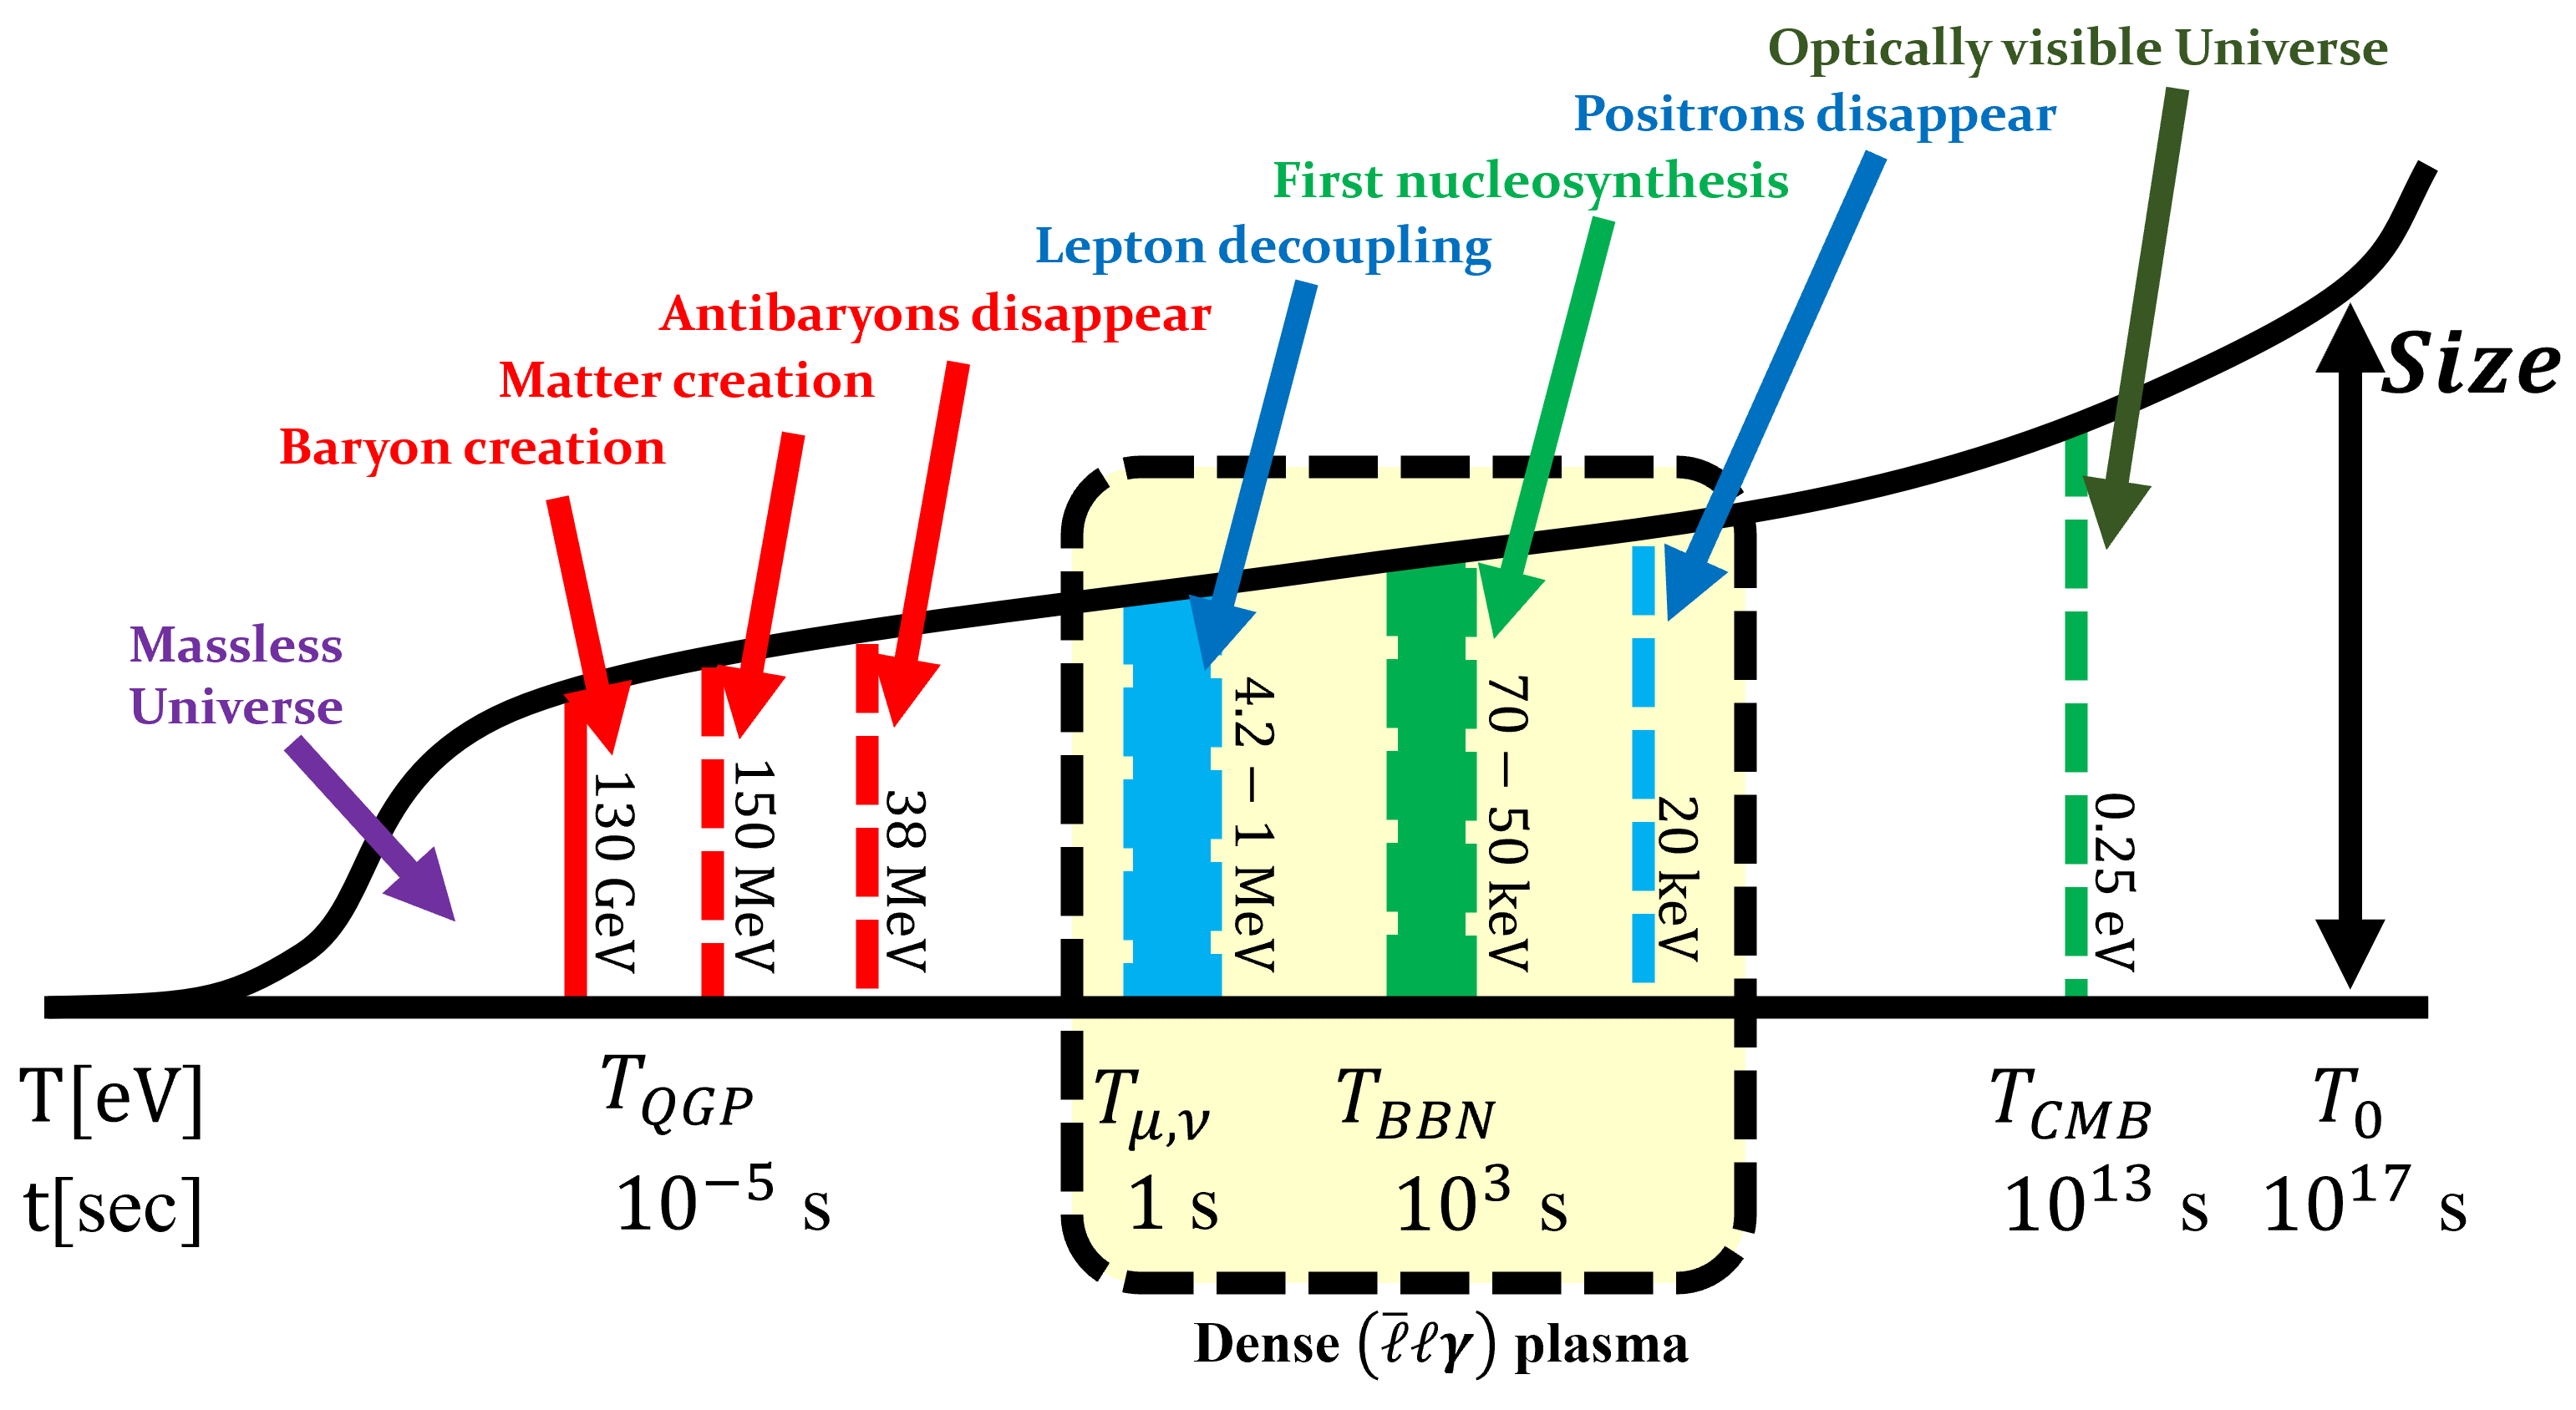
\includegraphics[width=0.95\linewidth]{plots/chap01intro/thesis_universe.png}
 \caption{A schematic of the universe's evolution since the Big Bang. The region of interest studied in this dissertation is emphasized (in the highlighted box) to contain a dense nearly charge neutral matter-antimatter plasma.}
 \label{fig:cosmo} 
\end{figure}
%%%%%%%%%%%%%%%%%%%%%%%%%%%%%%%%%%%%%%%

The scale factor $a(t)$ denotes the change of proper distances $L(t)$ over time as
\begin{gather}
    L(t)=L_{0}\frac{a_{0}}{a(t)}\rightarrow L(z)=L_{0}(1+z)\,,
\end{gather}
where $z$ is the redshift and $L_{0}$ the comoving length. In an expanding (or contracting) universe which is both homogeneous and isotropic. This implies volumes change with $V(t)=V_{0}/a^{3}(t)$ where $V_{0}=L_{0}^{3}$ is the comoving Cartesian volume. The evolutionary expansion of the universe is then traditionally defined in terms of the Hubble parameter $H(t)$ following the conventions in~\cite{weinberg1972gravitation}
\begin{gather}
  \label{Friedmann:1} H(t)^{2}\equiv\left(\frac{\dot a}{a}\right)^2=\frac{8\pi G_{N}}{3}\rho_\mathrm{total},\qquad \rho_\mathrm{total}(t)=\rho_{\Lambda}+\rho_\mathrm{DM}(t)+\rho_\mathrm{Baryons}(t)+\ldots\\
  \label{Friedmann:2}
  \frac{\ddot a}{a}=-qH^2,\qquad 
q\equiv -\frac{a\ddot a}{\dot a^2},\qquad \dot H=-H^2(1+q).
\end{gather}
where $G_N$ is the Newtonian constant of gravitation. \req{Friedmann:1} and \req{Friedmann:2} are also known as the Friedmann equations. The total density $\rho_\mathrm{total}$ is the sum of all contributions from any form of matter, radiation or field. This includes but is not limited to: dark energy $(\Lambda)$, dark matter (DM), baryons (B), leptons $(\ell,\nu)$ and photons $(\gamma)$. Depending on the age of the universe, the relative importance of each group changes as each dilutes differently under expansion with dark energy infamously remaining constant in density and accelerating the universe today.

The parameter $q$ is the cosmic deceleration which for historical reasons is positive $q>0$ under deceleration. This convention was chosen before the discovery of dark energy under the tacit assumption that the universe would be decelerating. The value of $q$ depends on energy content: The early universe was radiation dominated $(q = 1)$, subsequently matter dominated $(q = 1/2)$, and lastly the contemporary universe is undergoing a transition from matter to dark energy dominated approaching the asymptotic value of $q = -1$; see~\cite{Rafelski:2013yka}.

We can consider the expansion to be an adiabatic process~\cite{Abdalla:2022yfr} which results in a smooth shifting of the relevant dynamical quantities. As the universe undergoes isotropic expansion, the temperature decreases as 
\begin{gather}
 \label{tscale}
 T(t)=T_{0}\frac{a_{0}}{a(t)}\rightarrow T(z)=T_{0}(1+z)\,,
\end{gather}
where $z$ is the redshift. The entropy within a comoving volume is kept constant until gravitational collapse effects become relevant. The comoving temperature $T_{0}$ is given by the the present CMB temperature $T_{0}=2.7{\rm\ K}\simeq2.3\times10^{-4}\eV$~\cite{Planck:2018vyg}, with contemporary scale factor $a_{0}=1$.

As the universe expands, redshift reduces the momenta of particles lowering their contribution to the energy content of the universe. This cosmic redshift is written as
\begin{alignat}{1}
  \label{Redshift} p_{i}(t) = p_{i,0}\frac{a_{0}}{a(t)}\,.
\end{alignat}
Momentum (and the energy of massless particles $E=pc$) scales with the same factor as temperature. The energy of massive free particles in the universe however scales differently based on their momentum (and thus temperature).

When hot and relativistic, particle energy decreases inversely with scale factor like radiation. As the particles transition to non-relativistic (NR) energies, they decrease with the inverse square of the scale factor
\begin{alignat}{1}
    \label{EScale} E(t) = E_{0}\frac{a_{0}}{a(t)}\xrightarrow{\mathrm{NR}}\  E_{0}\frac{a_{0}^{2}}{a(t)^{2}}\,.
\end{alignat}
This occurs because of the functional dependence of energy on momentum in the relativistic $E\sim p$ versus non-relativistic $E\sim p^{2}$ cases.

\subsection{The standard FLRW-Universe model}
%In this section we will focus on the following:
%\begin{itemize}
%    \item The Robertson –Walker Universe
%    \item The Friedmann equation (Hubble %    \item The composition of the universe
%\end{itemize}
The Friedmann-Lemaitre-Robertson-Walker (FLRW) Universe is a theoretical model used widely to describe the cosmological evolution of the Universe. It is based on the cosmological principles which assumes homogeneity and isotropy of the Universe on large scales. In general, the FLRW metric can be written as
\begin{align}\label{metric}
ds^2=c^2dt^2-a^2(t)\left[ \frac{dr^2}{1-kr^2}+r^2(d\theta^2+\sin^2\theta\,d\phi^2)\right].
\end{align}
The metric is characterized by the scale factor $a(t)$ which measures the size of the Universe as a function of time $t$. The geometric parameter $k$ identifies the Gaussian geometry of the spatial hyper-surfaces defined by co-moving observers. The metrics are qualitatively different depending on the value of $k$. We have $k=1$ which correspond to the closed Universe,  $k=0$ correspond to flat Universe, and $k=-1$ for open geometries of the Universe. Current observation of cosmic microwave background (CMB) anisotropy preferred value $k=0$~[\cite{Planck:2013pxb,Planck:2015fie,Planck:2018vyg}].


The cosmological equations that describe the evolution of the Universe are derived from the Einstein equations. In general, the Einstein equation with cosmological constant $\Lambda$ can be written as:
\begin{equation}\label{Einstein}
  G^{\mu\nu}=R^{\mu\nu}-\left(\frac R 2 +\Lambda\right) g^{\mu\nu}=8\pi G_N T^{\mu\nu}, 
\quad R= g_{\mu\nu}R^{\mu\nu}.  
\end{equation}
where $G_{N}$ is the Newtonian gravitational constant, and $T^{\mu\nu}$ is the stress-energy tensor. Given the homogeneous and isotropic symmetry conditions imply that the matter context of the Universe can be expressed as a perfect fluid. The stress-energy tensor $T^\mu_\nu$ of perfect fluid can be written as
\begin{align}
 T^\mu_\nu =\mathrm{diag}(\rho, -P, -P, -P).
\end{align}
where $\rho$ is energy density and an $P$ is the isotropic pressure.

Substituting the perfect fluid form of the stress-energy tensor into the Einstein equations, one can derive the cosmological equations that describe the evolution of the Universe. We then obtain Friedmann equations as follows:
\begin{align}
\label{Hubble} 
&H^{2}\equiv\left(\frac{\dot a}{a}\right)^2=\frac{8\pi G_{N}}{3}\rho-\frac{k}{a^2}+\frac{\Lambda}{3},\\
\label{q_value}
&qH^2=\frac{4\pi G_{N}}{3}\left(\rho+3P\right)-\frac{\Lambda}{3},\qquad q\equiv -\frac{a\ddot a}{\dot a^2},
\end{align}
where $H$ is the Hubble parameter,  $q$ is the deceleration parameter. These equations relate the dynamics of the scale factor $a(t)$ to the energy density and pressure of the cosmic plasma. On the other hand, considering the divergence freedom of the total stress-energy tensor $\nabla_\nu T^{\mu\nu}=0$. For $\mu=0$ component, we have
\begin{align}\label{energy_eq}
\nabla_\nu T^{0\nu}=\frac{d\rho}{dt}+3H(\rho+P)=0
\end{align}
which provides dynamical evolution equation for $\rho(t)$ and $P(t)$. Solutions of Eq.~(\ref{energy_eq}) describes the time evolution of  energy density and pressures in the Universe. Given the energy density and pressure as a function of time, we can illustrates how the Universe evolves according to the Friedmann equations Eq.~(\ref{Hubble}) and Eq.~(\ref{q_value}). Solving these equations allows us to understand the dynamics and evolution of the Universe such as the Hubble expansion and the behavior of matter and energy over cosmic time.

\subsection{Cosmic plasma in early Universe $300\,\mathrm{MeV}>T>0.02\,\mathrm{MeV}$}
%In this section we will focus on the following:
%\begin{itemize}
%    \item Five different plasma epoch from $0.3\mathrm{GeV}>T>20$keV
%\end{itemize}

The primordial hot Universe fireball underwent several practically adiabatic phase changes that dramatically evolved its bulk properties as it expanded and cooled~[\cite{Rafelski:2023emw}]. We present an overview of the Universe evolution as a function of temperature from $300\,\mathrm{MeV}>T>0.02\,\mathrm{MeV}$ and main events constituting the history of the early Universe in Fig.~\ref{Overview_fig}. After the electroweak symmetry breaking epoch and presumably inflation, the comic plasma in the early Universe evolves in the following sequence:

%%%%%%%%%%%%%%%%%%%%%%%%%%%%%%%%%%%%%%%
\begin{figure}[ht]
 \centerline{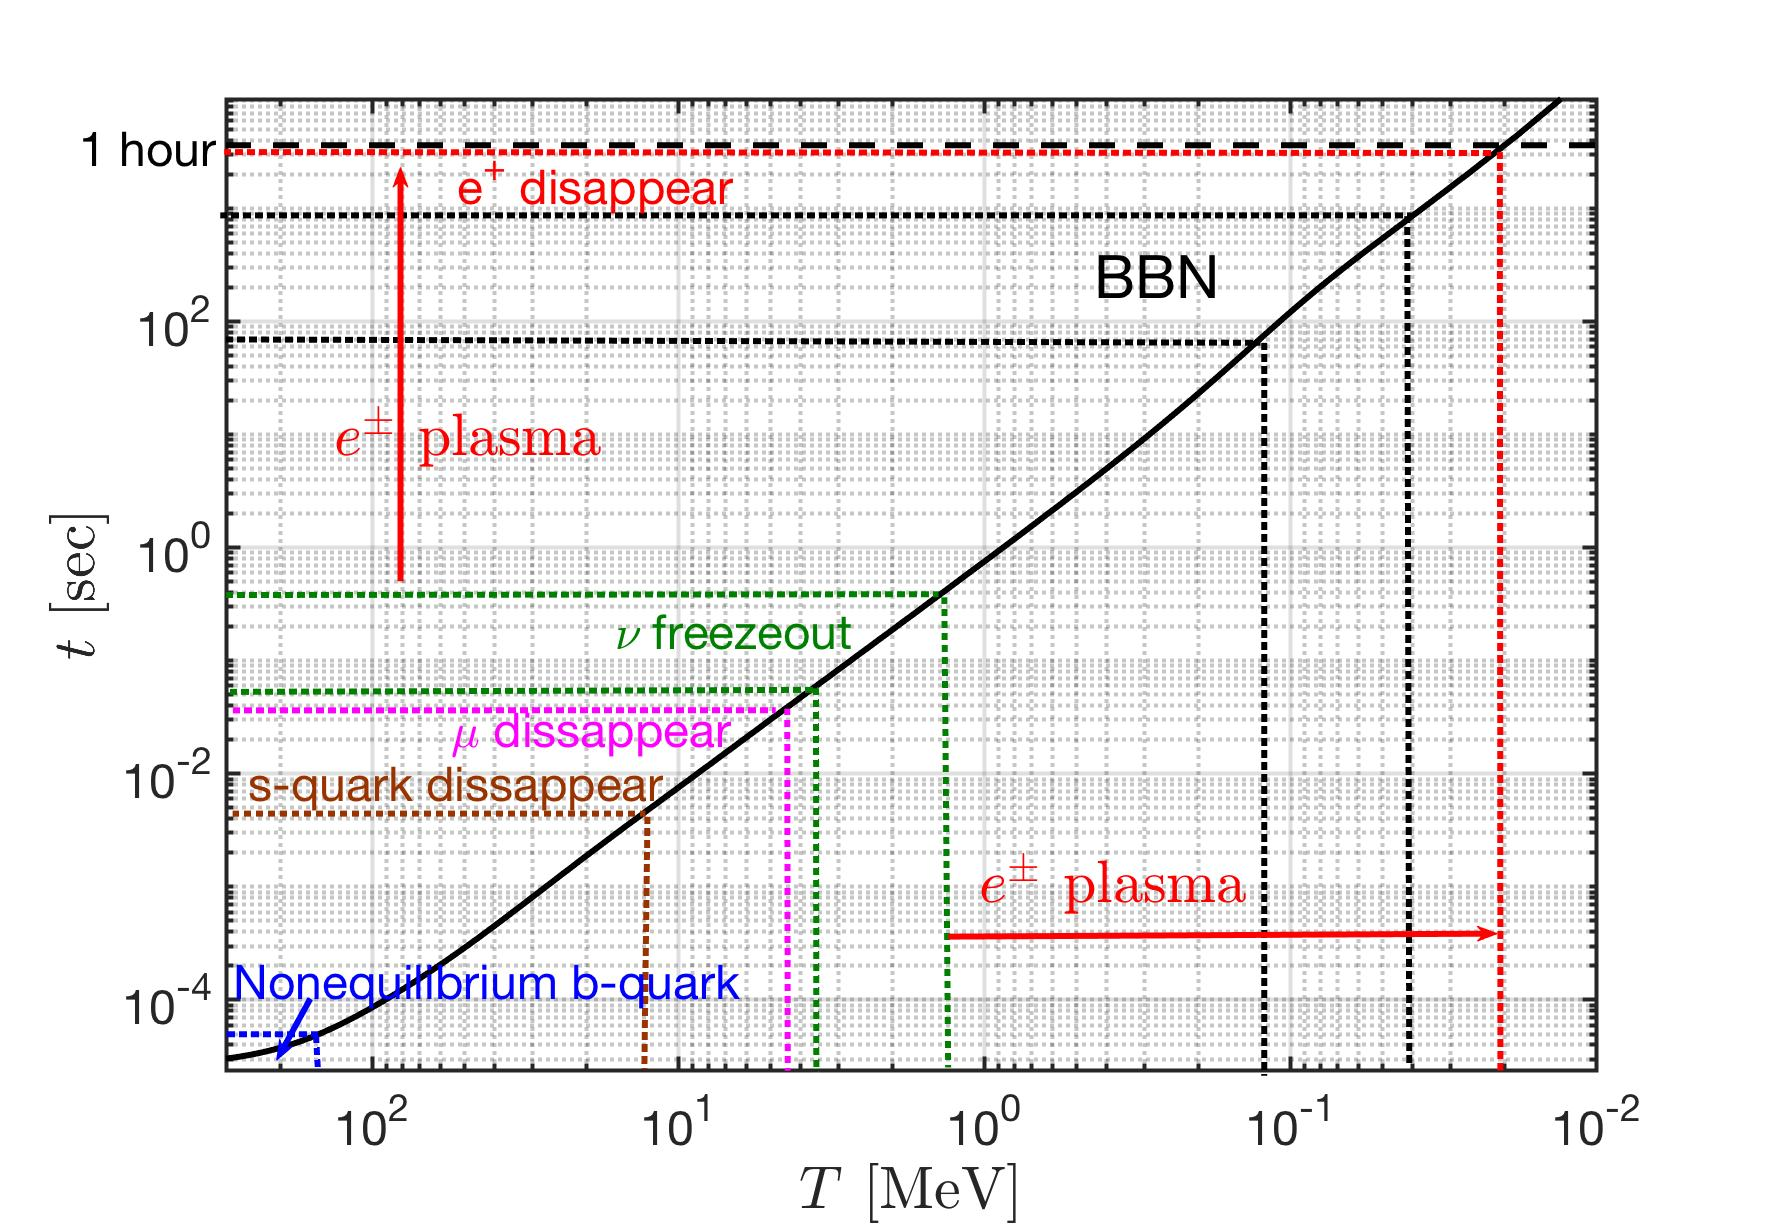
\includegraphics[width=\textwidth,width=\linewidth]{./plots/CosmicTimeTemperature_Project}}
 \caption{The time evolution of the early Universe as a function of temperature from $300\,\mathrm{MeV}>T>0.02\,\mathrm{MeV}$ and 
 different sequence of main events are shown with the temperature/time range in the evolution. }
 \label{Overview_fig}
\end{figure}
%%%%%%%%%%%%%%%%%%%%%%%%%%%%%%%%%%%%%%%

\begin{enumerate}
    \item \textbf{Primordial quark-gluon plasma}: 
    At early times when the temperature was between $130\,\mathrm{GeV}>T>0.15\,\mathrm{GeV}$ we have the building blocks of the Universe as we know them today, including the leptons, vector bosons, and all three families of deconfined quarks and gluons which propagated freely in plasma. As all hadrons are dissolved into their constituents during this time, strongly interacting particles $u,d,s,t,b,c,g$ controlled the fate of the Universe. When temperature is near to the QGP phase transition $300\, \mathrm{MeV}>T>150$ MeV, the bottom quark  breaks the detail balance and disappearance from particle inventory provides the arrow in time (see Chapter~\ref{Bottom} for detail).
    
    \item \textbf{Hadronic epoch}: Around the hadronization temperature $T_H\approx150\,\mathrm{MeV}$, a phase transformation occurred, forcing 
    the free quarks and gluons become confined within baryon and mesons [\cite{Letessier:2005qe}]. In the temperature range $ 150\,\mathrm{MeV}>T>20\,\mathrm{MeV}$, the Universe is rich in physics phenomena involving strange mesons and (anti)baryons including (anti)hyperon abundances~[\cite{Fromerth:2012fe,Yang:2021bko}]. The antibaryons disappear from the Universe at temperature $T=38.2$ MeV, and strangeness can be produced by the inverse decay reactions that are in equilibrium via weak, electromagnetic, and strong interactions in the early Universe until $T\approx13$ MeV (see Chapter~\ref{Strangeness} for detailed discussion).

    
    \item \textbf{Lepton-photon epoch}: For temperature $10\,\mathrm{MeV}>T>2\,\mathrm{MeV}$, the Universe contained relativistic electrons, positrons, photons, and three species of (anti)neutrinos. During this epoch massless leptons and photons controlled the fate of the Universe. Massive $\tau^\pm$ disappear from the plasma at high temperature via decay processes. However $\mu^\pm$ leptons can persist in the early Universe until temperature $T=4.2$ MeV, and positron $e^+$ can persist until the temperature $T=0.02$ MeV (See Chapter~\ref{Electron} for discussion).
    Neutrinos were still coupled to the charged leptons via the weak interaction~[\cite{Birrell:2012gg,Birrell:2014ona}] and freeze-out at temperature range $3\,\mathrm{MeV}>T>2\,\mathrm{MeV}$ which depends on the neutrino's flavors and the magnitude of the Standard Model parameters (See Chapter~\ref{Neutrino} for details). After neutrino freeze-out, they still play a important role in the Universe expansion via the effective number of neutrinos $N_{\nu}^{\mathrm{eff}}$ and affects the Hubble parameter significantly.  
    
    \item \textbf{Electron-positron epoch}: After neutrinos freeze-out at $T=3\sim2\,\mathrm{MeV}$ and become free-streaming in the early Universe, the cosmic plasma was dominated by electrons, positrons, and photons. The $e^\pm$ plasma existed until $T\approx0.02\,\mathrm{MeV}$ such that BBN occurred within a rich electron-positron plasma, and the dense number density of electron/positron also provide the opportunities to investigate magnetization process (See Chapter~\ref{Electron} for detailed discussion). This is the last time the Universe will contain a significant fraction of its content in antimatter.
\end{enumerate}
After $e^\pm$ annihilation, the Universe was still opaque to photons at this point and remained so until the recombination period at $T\approx0.25\,\mathrm{eV}$ starting the era of observational cosmology with the Cosmic Microwave Background. This period has been studied in detail before in~[\cite{Planck:2018vyg}]. Therefore, we focus on the temperature $300\,\mathrm{MeV}>T>0.02\,\mathrm{MeV}$ which corresponds to the first hour of the Universe evolution. We will address the cosmic plasma as follow: In Chapter~\ref{Bottom}, we discuss the heavy quarks (bottom/charm) abundance near to the QGP hadronization and show the nonequilibrium of bottom quark.  In Chapter~\ref{Strangeness} we study the strangeness abundance after hadronization and show the long lasting strangeness in the early Universe. In Chapter~\ref{Neutrino} we focus on the neutrino-matter interactions and the evolution of cosmic neutrino in early universe before/after freeze-out. In Chapter~\ref{Electron} we study the abundance of charged leptons $\mu^\pm$ and $e^\pm$ and show that the present of $e^\pm$ plasma plays an important role in early Universe. In Chapter~\ref{Outlook} we address the ongoing and prospective research projects for future publication.
Finally in Chapter~\ref{Summary} we summarize the important results of our study and conclusion.

\section{Introduction to Cosmology and the Relic Neutrino Background}\label{ch:intro}
At a temperature of $5$ MeV the Universe consisted of a plasma of $e^\pm$, photons, and neutrinos. At around $1$ MeV neutrinos stop interacting, or freeze-out, and begin to free-stream through the Universe. Today they comprise the relic neutrino background. Photons freeze-out around $0.25$ eV and today they make up the Cosmic Microwave Background (CMB), currently at $T_{\gamma,0}=0.235$ meV.  Relic neutrinos have not been directly measured, but their impact on the speed of expansion of the Universe is imprinted on the CMB.  Indirect measurements of the relic neutrino background, such as by the Planck satellite \cite{Planck},  constrain neutrino properties such as mass and number of massless degrees of freedom.

 In later chapters, we will study the details of the neutrino freeze-out process and their impact on observables in detail but first we present an overview of cosmology, from just prior to neutrino freeze-out until today, putting the relic neutrinos in their proper context. Much of this material, including most figures, was adapted from our paper \cite{ErasOfUniverse}.


\subsection{Standard Cosmology}\label{cosmo}
 To follow the history of the relic neutrino distribution, one must first understand the relation between the expansion dynamics of the Universe, its energy content, and the connection to the photon and neutrino temperature. For this purpose we need some preparation in the  Friedmann$-$Lemaitre$-$Robertson$-$Walker (FRW) cosmological  model, see for example \cite{hartle2003gravity,hobson,misner1973gravitation}. Assuming a homogeneous, isotropic Universe, one arrives at the spacetime metric
\beqn\label{metric}
ds^2=dt^2-a^2(t)\left[ \frac{dr^2}{1-kr^2}+r^2(d\theta^2+\sin^2(\theta)d\phi^2)\right]
%g_{00}=1, \quad g_{rr}=-\frac{a^2}{1-kr^2}, \quad g_{\theta\theta}=-a^2r^2, \quad g_{\phi\phi}=-a^2 r^2\sin^2\theta
\eeqn
characterized  by the scale parameter $a(t)$.  $a(t)$ determines the distance between objects at rest in the Universe frame, otherwise known as comoving observers. The geometric parameter $k=-1,0,1$ identifies the geometry of the spacial hypersurfaces defined by comoving observers. Space is a flat-sheet for the observationally preferred value $k=0$ \cite{Planck}, hyperbolic for $k=-1$, and spherical for $k=1$.

The dynamics are governed by the Einstein equations
\beqn\label{Einstine}
G^{\mu\nu}=R^{\mu\nu}-\left(\frac R 2 -\Lambda\right) g^{\mu\nu}=-\frac{1}{M_p^2} T^{\mu\nu},  
\quad R= g_{\mu\nu}R^{\mu\nu}
\eeqn
where $M_p\equiv 1/\sqrt{8\pi G_N}$ is the Planck mass, $G_N$ is the gravitational constant, and we work in units where $\hbar=c=1$. Recall that the Einstein tensor $G^{\mu\nu}$ is divergence free and hence so is the total stress energy tensor, $T^{\mu\nu}$.  Note that our definition of $M_p$, while more convenient in cosmology, differs by a factor of $1/\sqrt{8\pi}$ from the particle physics convention.  Finally, we point out that there are several sign conventions in use regarding the definition of geometrical quantities and Einstein's equation that are clarified in appendix \ref{app:conventions}.

 In a homogeneous isotropic spacetime, the matter content is necessarily characterized by two quantities, the energy density $\rho$ and isotropic pressure $P$
\begin{equation}
  T^\mu_\nu =\mathrm{diag}(\rho, -P, -P, -P).
\end{equation}
 It is common to absorb the Einstein cosmological constant $\Lambda$ into $\rho$ and $P$ by defining
\beqn\label{EpsLam}
\rho_\Lambda=M_p^2\Lambda, \qquad P_\Lambda=-M_p^2 \Lambda.
\eeqn
We implicitly consider this done from now on. 


The global Universe dynamics can be characterized by two  quantities, the Hubble parameter  $H$, a strongly time dependent quantity on cosmological time scales,  and the deceleration parameter $q$
\beqn\label{dynamic}
\frac{\dot a }{a}\equiv H(t) ,\quad 
q\equiv -\frac{a\ddot a}{\dot a^2}.
\eeqn
We note the relations
\beqn
\quad \frac{\ddot a}{a}=-qH^2,\quad \dot H=-H^2(1+q). 
\eeqn

Two dynamically independent equations arise using the metric \req{metric} in \req{Einstine}
\beqn\label{hubble}
\frac{8\pi G_N}{3} \rho =  \frac{\dot a^2+k}{a^2}
=H^2\left( 1+\frac { k }{\dot a^2}\right),
\qquad
\frac{4\pi G_N}{3} (\rho+3P)  =-\frac{\ddot a}{a}=qH^2.
\eeqn
We can eliminate the strength of the interaction, $G_N$,  solving both these equations for ${8\pi G_N}/{3}$, and equating the result to find a relatively simple constraint for the deceleration parameter
\beqn\label{qparam}
q=\frac 1 2 \left(1+3\frac{P}{\rho}\right)\left(1+\frac{k}{\dot a^2}\right).
\eeqn
 From this point on, we work within the  flat cosmological model with $k=0$ and so $q$ is determined entirely by the matter content of the Universe
\begin{equation}\label{qparam}
q=\frac 1 2 \left(1+3\frac{P}{\rho}\right).
\end{equation}


As must be the case for any solution of Einstein's equations,   \req{hubble} implies that the energy momentum tensor of matter is divergence free
\beqn\label{divTmn}
\nabla_\nu T^{\mu\nu} =0 \Rightarrow -\frac{\dot\rho}{\rho+P}=3\frac{\dot a}{a}=3H.
\eeqn
 The same relation also follows from  conservation of entropy, $dE+PdV=TdS=0,\  dE=d(\rho V),\  dV=d(a^3)$. Given an equation of state $P(\rho)$, solution of \req{divTmn} describes the dynamical evolution of matter in the Universe. Combined with the Hubble equation
\begin{equation}\label{Hubble_eq}
H^2=\frac{\rho}{3M_p}
\end{equation}
this allows us to solve for the large scale dynamics of the Universe. 

Using the flat FRW model of cosmology outlined above, we now present several perspectives on the history of the Universe.  First we focus on the reheating history. 

%%%%%%%%%%%%%%%%%%%%%%%%%%%%%%%%%%%%%%%%%%%%%%%%%%%%%%%%%%%%%%%
\subsection{Reheating History of the Universe}\label{Eralink}

At times where dimensional scales are irrelevant, entropy conservation means that  temperature scales inversely with the scale factor $a(t)$. This follows from \req{divTmn} when $ \rho\simeq 3P   \propto T^4$. However, as the temperature drops and at their respective $m\simeq T$ scales, successively less massive particles annihilate and disappear from the thermal Universe. Their entropy reheats the other degrees of freedom and thus in the process, the entropy originating in a massive degree of freedom is shifted into the effectively massless degrees of freedom that still remain.  This causes the  $T\propto 1/a(t)$ scaling to break down; during each of these `reorganization' periods the drop in temperature is slowed by the concentration of entropy in fewer degrees of freedom, leading to a change in the reheating ratio, $R$, defined as
\begin{equation}\label{redshiftratio}
R\equiv \frac{1+z}{ T_\gamma/T_{\gamma,0}}, \qquad 1+z\equiv \frac{a_{0}}{a(t)}.
\end{equation}
The reheating ratio connects the photon temperature redshift to the geometric redshift, where $a_0$ is the scale factor today (often normalized to $1$) and quantifies the deviation from the scaling relation between $a(t)$ and $T$.

As we will see, the change in $R$ can be computed by the drop in the number of degrees of freedom.  At a temperature on the order of the top quark mass, when all standard model particles were in thermal equilibrium, the Universe was pushed apart by 28 bosonic and 90 fermionic degrees of freedom. The total number of degrees of freedom can be computed as follows.  

For bosons we have the following: the doublet of charged Higgs particles has $4=2\times2=1+3$  degrees of freedom -- three will migrate to the longitudinal components of $W^\pm, Z$ when the electro-weak vacuum freezes and the EW symmetry breaking arises, while one is retained in the one single dynamical charge neutral Higgs component. In the massless stage, the SU(2)$\times$U(1) theory has 4$\times$2=8 gauge degrees of freedom where the first coefficient  is  the number of particles $(\gamma, Z, W^\pm)$ and each massless gauge boson has  two transverse polarizations. Adding in $8_c\times2_s=16$ gluonic degrees of freedom we obtain 4+8+16=28  bosonic degrees of freedom. 

The count of fermionic degrees of freedom includes three $f$ families, two spins $s$, another factor two for particle-antiparticle duality. We have in each family of flavors a doublet of $2\times 3_c$ quarks, 1-lepton and 1/2 neutrinos (due left-handedness which was not implemented counting spin). Thus we find that a total $3_f\times 2_p\times 2_s\times(2\times 3_c+1_l+1/2_\nu)=90$ fermionic degrees of freedom. We further recall that massless fermions contribute 7/8 of that of bosons in both pressure and energy density. Thus the total number of massless Standard Model particles at a temperature above the top quark mass scale, referring by convention to bosonic degrees of freedom, is $g_{\rm SM}=28+90\times 7/8=106.75$ 



In figure~\ref{fig:dof}  we show the cube of the reheating ratio \req{redshiftratio} as a function of photon temperature $T_\gamma$ from the primordial high temperature  early Universe on the right to the present on the left, where $R$  must be by definition unity.  The periods of change seen in figure \ref{fig:dof} come when the temperature crosses the mass of a particle species that is in equilibrium. One can see drops corresponding to the disappearance of particles as indicated.   After $e^+e^-$ annihilation on the left, there are no significant degrees of freedom remaining to annihilate and feed entropy into photons, and so $R$  remains constant until today. We show the result using a Fermi gas model with a very rough model for the QGP phase transition and hadronization period near $O(100\MeV)$. The fermi gas model is a poor approximation above the QGP phase transition; a more precise model using lattice QCD, see e.g. \cite{Borsanyi:2013bia}, together with a high temperature perturbative QCD expansion, see e.g. \cite{letessier2002hadrons}, would be needed to improve on this situation but the details do not impact the neutrino freeze-out period near $1\MeV$ which is our primary concern, and so we do not consider these issues further here.

%%%%%%%%%%%%%%%%%%%%%%%%%%%%%%%%%%%%%%%
\begin{figure} 
\centerline{\hspace*{0.4cm}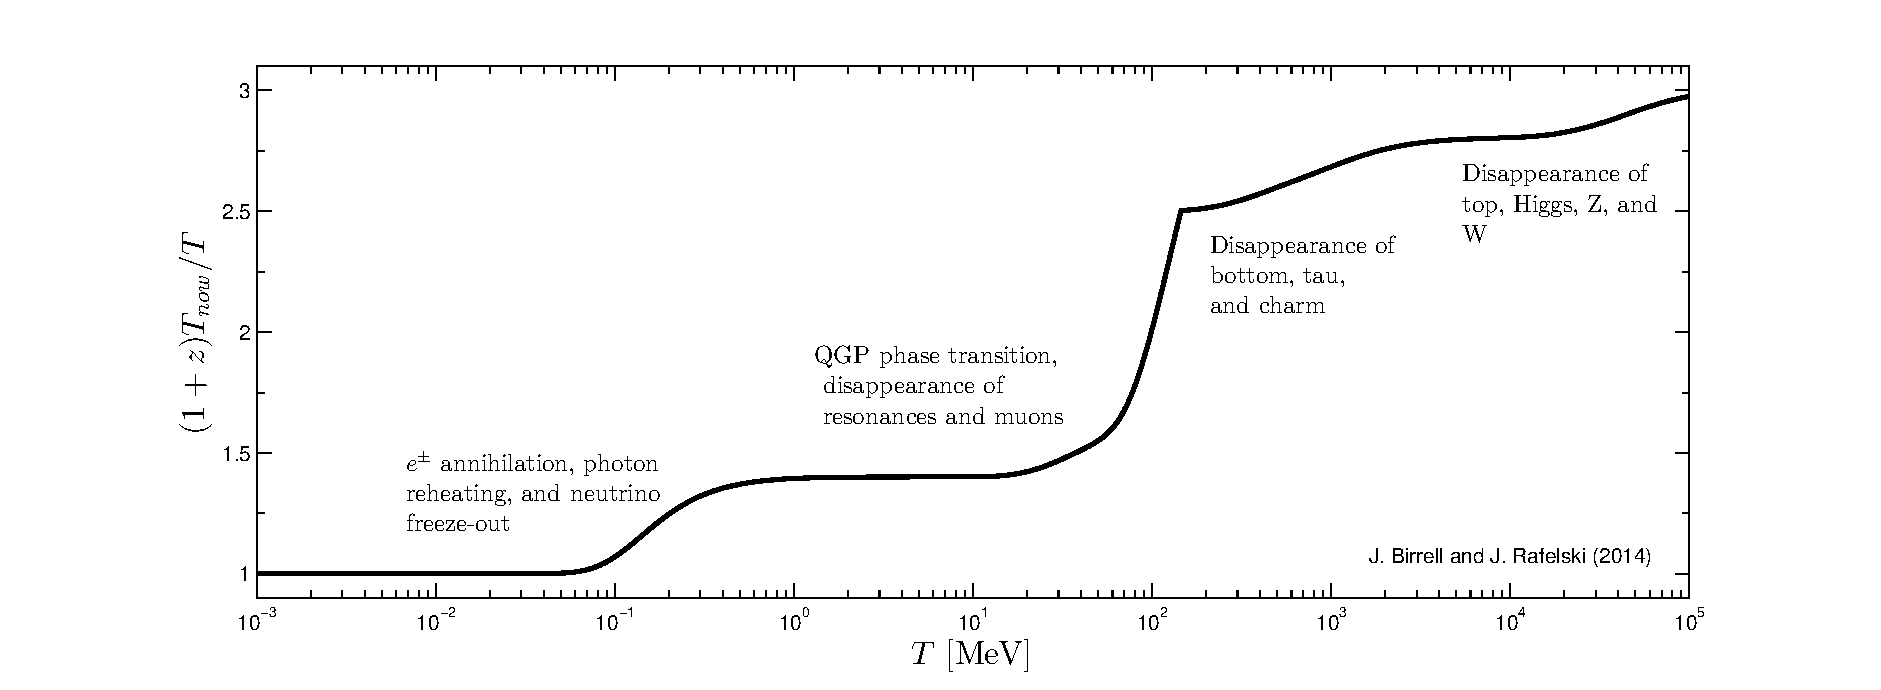
\includegraphics[height=6.6cm]{03-birrell/ErasOfUniverse/z_T_plot.eps}}
\caption{Disappearance of degrees of freedom. The Universe volume inflated approximately by a factor of 27 above the thermal red shift scale as massive particles disappeared successively from the inventory.\label{fig:dof}}
 \end{figure}
%%%%%%%%%%%%%%%%%%%%%%%%%%%%%%%%%%%%%%%



As long as the dynamics are at least approximately entropy conserving, the total drop in $R$ is entirely determined by entropy conservation. Namely, the magnitude of the drop in $R$ figure~\ref{fig:dof} is a measure of the number of degrees of freedom that have disappeared from the Universe. Consider   two times $t_1$ and $t_2$ at which all particle species that have not yet annihilated are effectively massless.  By conservation of comoving entropy and  scaling $T\propto 1/a$ we have
\begin{equation}\label{r_ratio}
1=\frac{a_1^3S_{1}}{a_2^3 S_2}=\frac{a_1^3\sum_ig_i T_{i,1}^3}{a_2^3\sum_j g_j T_{j,2}^3},\qquad \left(\frac{R_1}{R_2}\right)^3=\frac{\sum_ig_i (T_{i,1}/T_{\gamma,1})^3}{\sum_j g_j (T_{j,2}/T_{\gamma,2})^3}
\end{equation}
where the sums are over the total number of degrees of freedom present at the indicated time and the degeneracy factors $g_i$ contain the $7/8$ factor for fermions. In the second form    we divided the numerator and denominator by $a_{0}T_{\gamma,0}$. We distinguish between the temperature of each particle species and our reference temperature, the photon temperature.  This is important since today neutrinos are colder than photons, due to photon reheating from  $e^\pm$ annihilation occurring after neutrinos decoupled (this is only an approximation, a point we will study in detail in subsequent chapters).  By conservation of entropy one obtains the neutrino to photon temperature ratio of
\begin{equation}\label{T_nu_T_gamma}
T_\nu/T_\gamma=({4}/{11})^{1/3}.
\end{equation}
We will call this the reheating ratio in the decoupled limit.  For details on the derivation of this standard result, see for example our paper in appendix \ref{app:model_ind}, where it is obtained as a special case of a more general analysis. 

Using \req{r_ratio}  we  compute the total drop in $R^3$ shown in figure \ref{fig:dof}.  At $T=T_\gamma=\mathcal{O}(100\GeV)$ the number of active degrees of freedom is slightly below $g_{\rm SM}=106.75$ due to the partial disappearance of top quarks, but this approximation will be good enough for our purposes.  At this time, all the species are in thermal equilibrium with photons and so $T_{i,1}/T_{\gamma,1}=1$ for all $i$.  Today we have $2$ photon and $7/8\times 6$ neutrino degrees of freedom and a  neutrino to photon temperature ratio \req{T_nu_T_gamma}.  Therefore we have
\begin{equation}
\left(\frac{R_{100GeV}}{R_{now}}\right)^3= \frac{g_{SM}}{g_{\rm now}}=\frac{106.75}{2+\frac{7}{8}\times 6\times \frac{4}{11}}\approx 27.3
\end{equation}
which is the  fractional change we see in the fermi gas model curve in figure \ref{fig:dof} (as mentioned above, the QCD model is reduced due to interactions). The meaning of this factor is that the Universe approximately inflated by a factor 27 above the thermal red shift scale as massive particles disappeared successively from the inventory. 


\subsection{Composition of the Universe}
From the perspective of reheating, the history of the Universe from the end of $e^\pm$ annihilation until today has been uneventful.  We can shed additional light on this period and others by looking at the composition of the Universe as a function of temperature

%%%%%%%%%%%%%%%%%%%%%%%%%%%%%%%%%%%%
\begin{figure}
\centerline{\hspace*{0.4cm}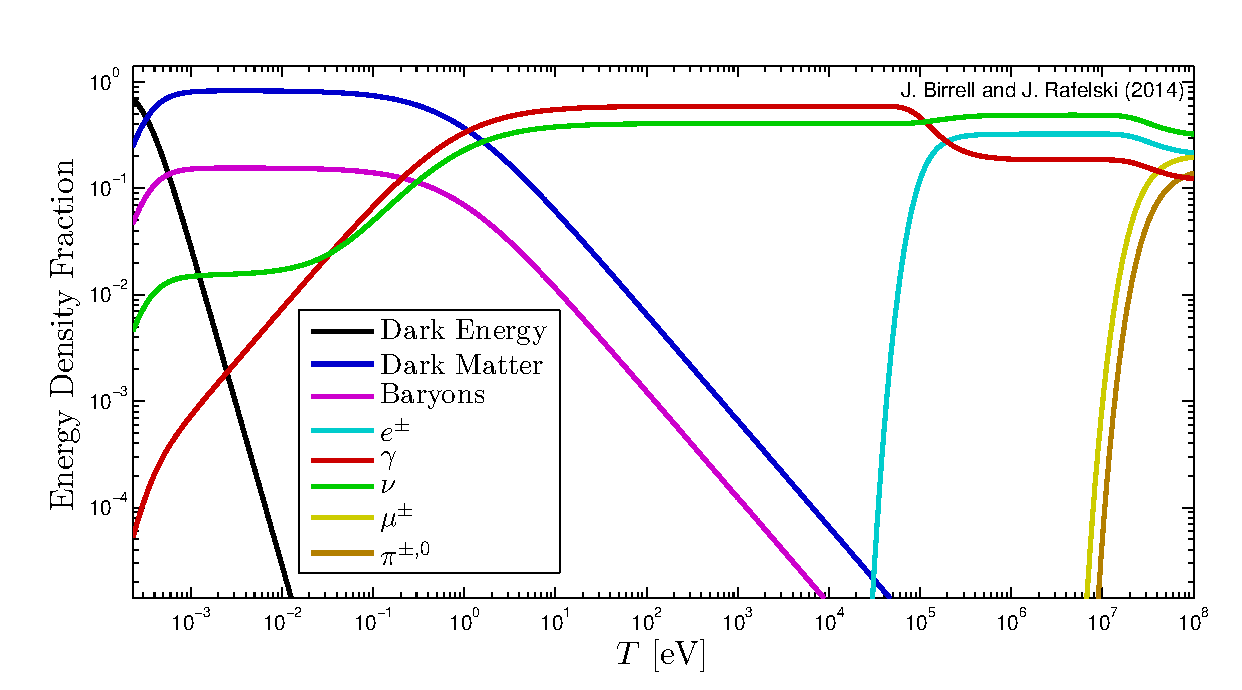
\includegraphics[height=7.6cm]{03-birrell/ErasOfUniverse/energy_densities_total.eps}}\label{fig:energy_frac}
\caption{Current era: $69\%$ dark energy, $26\%$ dark matter, $5\%$ baryons, $<1\%$ photons and neutrinos, $1$ massless and $2\times .1$ eV neutrinos (Neutrino mass choice is just for illustration.  Other values are possible).}
 \end{figure}
%%%%%%%%%%%%%%%%%%%%%%%%%%%%%%%%%%
In figure \ref{fig:energy_frac} we begin on the right at the end of the hadron era with the disappearance of muons and pions.  This constitutes a reheating period, with energy and entropy from these particles being transfered to the remaining $e^\pm$, photon, neutrino plasma.  Continuing to $T=O(1)$ MeV, we come to the annihilation  of $e^\pm$ and the photon reheating period.  Notice that only the photon energy density fraction increases here.  As discussed above, a common simplifying assumption is that neutrinos are already decoupled at this time and hence do not share in the reheating process, leading to a difference in photon and neutrino temperatures \req{T_nu_T_gamma}.

After passing through a long period, from $T=O(1)$ MeV until $T=O(1)$ eV, where the energy density is dominated by photons and free-streaming neutrinos, we then come to the beginning of the matter dominated regime, where the energy density is dominated by dark matter and baryonic matter.  This transition is the result of the redshifting of the photon and neutrino energy, $\rho\propto T^4$, whereas for non-relativistic matter $\rho\propto a^{-3}\propto T^3$.  Note that our inclusion of neutrino mass causes the leveling out of the neutrino energy density fraction during this period, as compared to the continued redshifting of the photon energy.

Finally, as we move towards the present day CMB temperature of $T_{\gamma,0}=0.235$ meV on the left hand side, we have entered the dark energy dominated regime.  For the present day values, we have used the fits from the Planck data \cite{Planck} of  $69\%$ dark energy, $26\%$ dark matter and $5\%$ baryons (and zero spatial curvature).  The photon energy density is fixed by the CMB temperature $T_{\gamma,0}$ and the neutrino energy density is fixed by $T_{\gamma,0}$ along with the photon to neutrino temperature ratio.  Both constitute $<1\%$ of the current energy budget.
%%%%%%%%%%%%%%%%%%%%%%%%
% Chapters from Cheng Tao Yang's dissertation SOME COMBINED and heavily edited JR
\section{Quark and Hadron Universe}\label{part2}
%%%%%%%%%%%%%%%%%%%%%%%%%%%%%%%%%%%%%%%%%
\subsection{Heavy particles in QGP epoch}
\label{HiggsQGP}
%%%%%%%%%%%%%%%%%%%%%%%%%%%%%%%%%%%%
\para{Matter phases in extreme conditions}
This section will be focused on a few examples of interest to cosmological context. In the temperature domain below electroweak boundary near $T=130$\,GeV we explore in preliminary fashion novel and interesting physical processes. We will consider the Higgs meson and the heavy quarks $t,b,c$ with emphasis on bottom quarks. We will show that the bottom quarks can deviate from chemical equilibrium $\Upsilon\neq 1$ by breaking the detailed balance between production and decay reactions. It is easy to see considering temperature scaling and additional degrees of freedom that the energy density of matter near to electroweak phase transition is a stunning 12 orders of magnitude greater compared to the benchmark we discussed for QGP-hadronization, see~\req{endensval}.
 
The dynamical bottom $ b,\bar b$-quark pair abundance depends on the competition between the strong interaction two gluon fusion process into $b\bar b$-pair and weak interaction decay rate of these heavy quarks. This lead to the off-equilibrium phenomenon of the bottom quark freeze-out in abundance near the hadronization temperature as discussed in Ref.\,\cite{Yang:2020nne} and below. Here we further argue that the same unusual situation could exist for any other heavy particle in QGP at a temperature well below their mass scale. We study as an example the abundance of the Higgs particle at condition $m_H\gg T$. Higgs is a particularly interesting case due to its special position in the particle ZOO and a narrow width.

We also explore the properties of hadronic phase after hadronization with special emphasis on gaining an understanding about the strangeness $s,\bar s$ content of the Universe which persists to unexpectedly low temperature. Many of the methods we use in this context were developed in order to understand the properties of strongly interacting QGP formed in relativistic \ie\ high-energy heavy-ion \ie\ nuclear collision experiments. Such experimental program is in progress at the Relativistic Heavy Ion Collider (RHIC) at BNL-New York\index{BNL!RHIC} and the Large Hadron Collider (LHC) at CERN\index{CERN!LHC}. 

Let us remind the reasons why the dynamics of particles and plasma in the primordial Universe differs greatly from the laboratory environment. We focus here on the case of QGP-hadron phase boundary but a similar tabular list applies to other era boundaries:\index{Big-Bang!difference with laboratory}
\begin{enumerate} 
\item The primordial Big-Bang QGP epoch lasts for about $20\,\mu$s. On the other hand, the QGP formed in collision micro-bangs has a lifespan of around $10^{-23}$\,s. 
\item In the primordial Universe the microscopic transformation of quarks into hadrons proceeded through creation of the so called mixed phase allowing for local equilibration and a full relaxation of strongly interacting degrees of freedom during about $10\,\mu$s~\cite{Fromerth:2002wb}. Current lattice QCD models predict a smooth transformation. The transformation in the laboratory is much closer to what can be called explosive and sudden conversion of quarks into hadronic (confined) degrees of freedom~\cite{Rafelski:2000by}. Such a situation can mimic phenomena usually observed in a true phase transition of first order.
\item Half of the degrees of freedom present in the Universe (charged leptons, photons, neutrinos) are not part of the thermal laboratory micro-bang.
\item Experimental reach today is at and below $T\simeq 0.5$\,GeV allowing to explore the hadronization process of the QGP but not the heavy particle (H,W,Z,$t$) content, $b$ and $c$ quarks are difficult to study. 
\item Though the baryon content of the laboratory QGP is very low it is probably also much higher compared to the observed baryon asymmetry in the Universe. 
\end{enumerate}
 
%%%%%%%%%%%%%%%%%%%%%%%%%%%%%%%%%%%
\para{Higgs equilibrium abundance in QGP} 
We would like to show that it is of interest to study the Higgs particle dynamics at relatively late stage of Universe evolution. This is an ongoing project which is described here for the first time. We are now considering in the primordial Universe the temperature range $10\,\mathrm{GeV}>T>1\,\mathrm{GeV}$, and recall the mass of the Higgs particle $m_H\simeq 125\GeV$. Therefore the number density of the Higgs can be written using the relativistic Boltzmann limit
\begin{align}
n_{H}=\frac{\Upsilon_H}{2\pi^2}T^3\left(\frac{m_H}{T}\right)^2 K_2(m_H/T)\,.
\end{align}\index{Higgs!particle abundance}

We are interested to compare the abundance of the Higgs particle to the net abundance of baryon excess over antibaryons to determine at which temperature the Higgs particle yield drops below this tiny Universe asymmetry. Our interest derives from the question how far down in temperature a baryon number breaking Higgs decay could be of relevance. Clearly, once the Higgs yield falls far below baryon asymmetry it would be difficult to argue it can contribute to grow the baryon asymmetry in the Universe. Moreover, comparing to baryon asymmetry seems to be a reliable measure of more general physical relevance, after all, our present Universe structure derives from this small asymmetry probably developed in the primordial epoch we explore here. 
 
The density between Higgs and baryon asymmetry (quark-antiquark asymmetry) can be written as
\begin{align}
\frac{n_H}{(n_B-n_{\bar{B}})}=\frac{n_{H}}{s_{tot}}\,\left(\frac{s_{tot}}{n_B-n_{\bar{B}}}\right)=
\frac{n_{H}}{s_{tot}}\left[\frac{s_{\gamma,\nu}}{n_B-n_{\bar{B}}}\right]_{t_0}\,.
\end{align}
Assuming no `late' baryon genesis and entropy conserving Universe expansion, we introduce in \req{BaryonEntropyRatio} in the last equality the present day value of baryon per entropy ratio. The entropy density $s_{tot}$ in QGP can be obtained employing the entropic degrees of freedom $g^s_\ast$, \req{eq:entg} and~\rf{EntropyDOF:Fig}
\begin{align}
 &s_{tot}=\frac{2\pi^2}{45}g^s_\ast T_\gamma^3,\qquad g^s_\ast=\sum_{i=\mathrm{g},\gamma}g_i\left({\frac{T_i}{T_\gamma}}\right)^3+\frac{7}{8}\sum_{i=l^\pm,\nu,u,d}g_i\left({\frac{T_i}{T_\gamma}}\right)^3\,.
\end{align}
The entropy content to a good approximation is dominated by all effectively massless particles at given temperature in QGP. 

The baryon-to-photon density ratio $\eta$ today is bracketed by $5.8\times10^{-10} \leqslant\eta\leqslant6.5\times10^{-10}$ \cite{ParticleDataGroup:2018ovx}, a more precise value $\eta=(6.12\pm0.04)\times10^{-10}$~\cite{ParticleDataGroup:2022pth} is used in our study. This observed value is the evidence of baryon asymmetry and quantifies the matter-antimatter asymmetry in the Universe.\index{baryon!photon ratio}

The density ratio between Higgs and baryon asymmetry for the case of chemical equilibrium $\Upsilon_H=1$ is seen in~\rf{HiggsDensity:fig}. At temperature $T=5.7\GeV$ this ratio is equal to unity. This implies that Higgs decay processes could populate and influence the baryon asymmetry down to this relatively low temperature scale. 

%%%%%%%%%%%%%%%%%%%%%%%%%%%%%%%%%%%%%%%%%%%%%%%%%%%%%%%%%%%%%%%%%%
\begin{figure}
\centerline{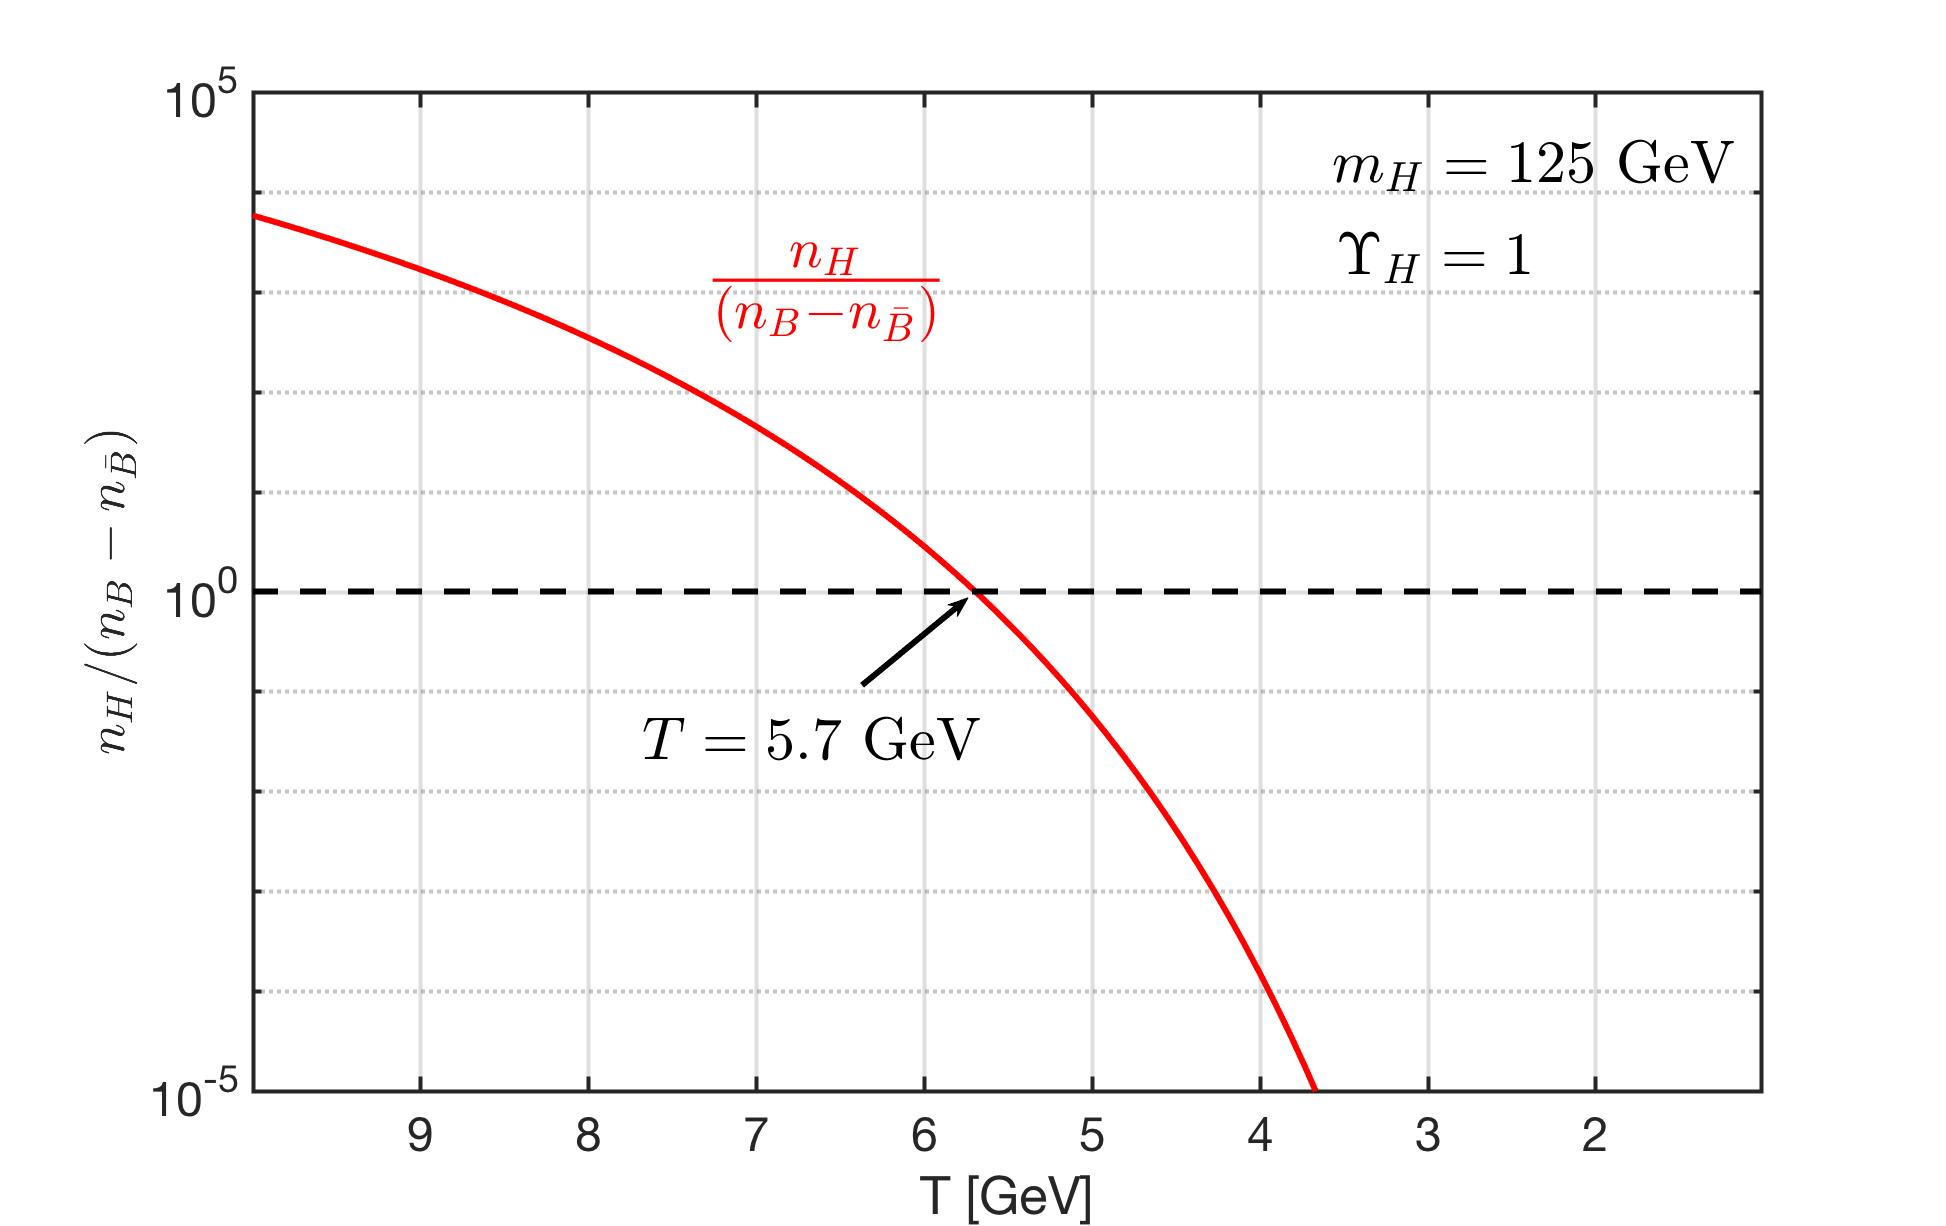
\includegraphics[width=0.9\linewidth]{./plots/HiggsDensityRatio}}
\caption{The ratio between Higgs density $n_H$ and baryon asymmetry density $n_B-n_{\bar B}$ as a function of temperature $T$ assuming chemical Higgs equilibrium $\Upsilon_H=1$ and present day entropy per baryon. Both densities are equal (horizontal line) at the temperature $T=5.7\GeV$. \radapt{Yang:2024ret}}
\label{HiggsDensity:fig} 
\end{figure}
%%%%%%%%%%%%%%%%%%%%%%%%%%%%%%%%%%%%%%%%%%%%%%%%%%%%%%%%%%%%%%%%%%%

%%%%%%%%%%%%%%%%%%%%%%%%%%%%
\para{Baryon asymmetry and Sakhraov conditions}\index{Sakharov conditions!baryogenesis}
The small value of the baryon asymmetry in the Universe could be interpreted as simply due to the initial conditions in the Universe. However, in the current standard cosmological model, it is believed that the inflation event can erase any pre-existing asymmetry between baryons and anti-baryons. In this case, we need a dynamic baryogenesis process to generate excess of baryon number compared to anti-baryon number in order to create the observed baryon number today.

The precise epoch responsible for the observed matter genesis $\eta$ in the primordial Universe has not been established yet. Several mechanisms have been proposed to explain baryogenesis with investigations typically focusing on the temperature range between GUT phase transition $T_\mathrm{G}\simeq10^{16}\,\mathrm{GeV}$ and the electroweak phase transition near $T_\mathrm{W}\simeq130\,\mathrm{GeV}$~\cite{Kuzmin:1985mm,Kuzmin:1987wn,Arnold:1987mh,Kolb:1996jt,Riotto:1999yt,Nielsen:2001fy,Giudice:2003jh,Davidson:2008bu,Morrissey:2012db}.

In following we present arguments that the Sakharov conditions~\cite{Sakharov:1967dj} for matter asymmetry to form also could appear during the QGP era: several heavy particles such as bottom quarks and including the Higgs as described above can fulfill nonequilibrium requirement. We will study below in more detail the bottom case and argue for the Higgs case. Other cases are possible.

In 1967, Andrei Sakharov formulated the three conditions necessary to permit baryogenesis in the primordial Universe~\cite{Sakharov:1967dj} and in 1991 he refined the three conditions as follows~\cite{Sakharov:1988vdp}:
\begin{itemize}
 \item Absence of baryonic charge conservation 
 \item Violation of CP-invariance
 \item Non-stationary conditions in absence of local thermodynamic equilibrium
\end{itemize}
 
In regard to first Sakharov condition: By assumption there is no initial asymmetry in baryon number in the Universe. Toady it is argued that an initial asymmetry could not survive the inflationary expansion. Furthermore ad-hoc Big-Bang baryon-antibaryon inherent asymmetry seems less attractive. In short we believe that the asymmetry between baryons and anti-baryons we observe requires dynamic process and the presence of baryon number non-conserving reactions. 

The other option, an interaction which favors agglomerations of same `sign' baryonic matter creating large domains in the Universe with small baryon-antibaryon asymmetry has never taken hold: We recall that the laws of physics favor opposite outcome, the elementary antimatter is eclectically attracted to matter. Neutral composite baryonic particles present in era in which antimatter is present (e.g. neutrons, $\Lambda(uds)$, charmed baryons etc., emerging just after QGP hadronization) deserve a second look on this account.

The second Sakharov condition requiring $CP$ violation assures us that we can recognize in universal manner the difference between matter and antimatter. Clearly, we could not enhance one form with reference to the other without being able to tell matter from antimatter. CP violation is allowing us to share with another distant civilization that we are made of matter. A nice textbook discussion showing how to do this using Kaon system CP violation is offered by Perkins~\cite{Perkins:1982xb}.

The third Sakharov condition is a requirement for breaking of detailed balance condition: It is evident that in thermal equilibrium, the net effect of baryogenesis processes is cancelled out by the detailed balance between forward and back-reactions. Space-time domains involving phase transitions harbor nonequilibrium thermal distributions leading to breaking of detailed balance. So far efforts to create consistent description of baryogenesis based on well studied electro-weak phase transition near $T=130$\,GeV has not been able to generate the observed baryon asymmetry. 

We distinguish kinetic (momentum distribution) and chemical (particle abundance) equilibrium. This is so since kinetic equilibrium is usually established much more quickly, while abundance yields are more difficult to establish, especially so for particles with masses in excess, or at least similar to ambient temperatures~\cite{Koch:1986ud,Birrell:2014gea}. This distinction has two relevant consequences: a) Detailed balance can arise also outside of strict chemical equilibrium condition which is seen in other physical environments, including the nucleo-synthesis processes in the Universe (BBN) and stars. b) There is a long lasting small violation of detailed balance related to the arrow of time introduced by the Universe expansion. c) Most promissing is for absence of stationary distribution is lack of kinetic equilibrium. 

Specifically for all heavy primordial particles including the top $t$ and bottom $b$ quarks, W and Z gauge bosons, and, the Higgs particle H we observe that when the Universe expands and temperature cools down well below the particle mass, the production process and decay processes create a stationary equilibrium with detailed balance outside of equilibrium. However, Universe expansion disturbs this creating non-stationary effects. Moreover, as we will argue just below, Higgs is an excellent candidate for non-stationary effects due to its small coupling to low mass particle plasma. Thus we interpret the third condition of Sakharov in our specific context as follows:
\begin{itemize}
\item Non-stationary conditions in absence of local thermodynamic equilibrium $\Longrightarrow$ Absence of detailed balance associated with nonequilibrium yields and non-stationary particle momentum abundance evolution.
\end{itemize} 

We believe that the presence of chemical (abundance) nonequilibrium is a required condition for baryogenesis environment which extends the phenomenon to a much wider temperture domain beyond the electro-weak phase transition condition down to a temperature of a few GeV. This is one of our ongoing research challenges. We will use the case of bottom quarks to demonstrate the mechanism we are exploring.
 
%%%%%%%%%%%%%%%%%%%%%%%%%%%%%%%
\para{Production and decay of Higgs in QGP}
The Higgs particle is unique among heavy PP-SM particles also due to its stability: The total width is $\Gamma_H\simeq 2.5\,10^{-5}M_H$. This combines with the unexpected low value of $T=5.7\GeV$ of interest where the Higgs yield equals to the baryon asymmetry in the Universe. This motivates us to examine here in qualitative manner the dynamical abundance of the Higgs particle in the QGP epoch, seeking eventual non-stationary condition needed for baryogenesis 

The Higgs predominantly decays via the $W,Z$ decay channels as follows:
\begin{align}
H\longrightarrow WW^\ast\,. ZZ^\ast\longrightarrow\mathrm{anything}\,.
\end{align}
Here $W^\ast,Z^\ast$ represent the production of virtual off-mass-shell gauge bosons decaying rapidly into relevant particle pairs. Therefore once Higgs decays via this channel at least four particles are ultimately formed and there is no path back for $T\ll m_H$. This is so since the spectral energy of produced particles, $31\GeV$ is highly epithermal compared to the ambient plasma at the low temperature of interest near to $T\simeq 6\GeV$. Therefore a back-reaction production of Higgs cannot be in balance for chemical equilibrium yield. 

In the QGP epoch, the dominant production of the Higgs boson is the bottom quark pair fusion reaction: 
\begin{align}
b+\overline{b}\longrightarrow H\,,
\end{align}
which is the inverse to the important but by far not dominant decay process of $H\to b+\overline{b}$. This means that in first approximation the detailed balance Higgs yield is reached well below the chemical equilibrium.

However, there could be considerable deviation from kinetic momentum equilibrium as well. This is so since bottom fusion will in general produce a Higgs particle out of kinetic momentum equilibrium. A heavy particle immersed into a plasma of lighter particles requires many, many collisions to equilibrate the momentum distribution. This is a well known kinetic theory result. Moreover, the Higgs particle interacts weakly with all lower mass particles in QGP present at $T<10\GeV$. 

Higgs particle is by far the best candidate to fulfill the Sakharov non-stationary condition in the primordial Universe at a temperature range of interest to baryogenesis. A full dynamic study leading to proper understanding of the off-chemical and off-kinetic equilibrium non-stationary abundance of Higgs is one of near future projects we consider and is beyond the scope of this report. 

%%%%%%%%%%%%%%%%%%%%%%%%%%%%%%%%
\subsection{Heavy quark production and decay}
\label{sec:heavyQ}
%%%%%%%%%%%%%%%%%%%%%%%%%%%%%%%%%
\para{Heavy quarks in primordial QGP}\index{quark!abundance}
The primordial quark-gluon plasma (QGP) refers to the state of matter that existed in the primordial Universe, specifically for time $t\approx 20\, \mathrm{\mu s}$ after the Big Bang. At that time the Universe was controlled by the strongly interacting particles: quarks and gluons. In this chapter, we study the heavy bottom and charm flavor quarks near to the QGP hadronization temperature $0.3\,\mathrm{GeV}>T>0.15\,\mathrm{GeV}$ and examine the relaxation time for the production and decay of bottom/charm quarks then show that the bottom quark nonequliibrium occur near to QGP–hadronization and create the arrow in time in the primordial Universe.
 
In the QGP epoch, up and down $(u,d)$ (anti)quarks are effectively massless and provide along with gluons, some leptons, and photons the thermal bath defining the thermal temperature. Strange $(s)$ (anti)quarks are also found to be in equilibrium considering their weak, electromagnetic, and strong interactions, indeed this equilibrium continues in hadronic epoch until $T\approx13\MeV$~\cite{Yang:2021bko}. 

The massive top $(t)$ (anti)quarks couple to the plasma via the channel~\cite{ParticleDataGroup:2018ovx}
\begin{equation}
t\leftrightarrow W+b\,,\qquad \Gamma_t=1.4\pm0.2\,\mathrm{GeV}\,.
\end{equation}
As is well known, the width prevents formation of bound toponium states. Given the large value of $\Gamma_t$ there is no freeze-out of top quarks until $W$ itself freezes out. To address the top quarks in QGP, a dynamic theory for $W$ abundance is needed, a topic we will embark on in the future. 
 
The semi-heavy bottom $(b)$ and charm $(c)$ quarks can be produced by strong interactions via quark-gluon pair fusion processes, these quarks decay via weak interaction decays, their abundance depends on the competition between the strong interaction fusion processes at low temperature inhibited by the mass threshold, and weak decay reaction rates.

In the following we consider the temperature near QGP hadronization $0.3\,\mathrm{GeV}>T>0.15\,\mathrm{GeV}$, and study the bottom and charm abundance by examining the relevant reaction rates of their production and decay.
In thermal equilibrium the number density of light quarks can be evaluated in the massless limit, and we have\index{number density of quark}
\begin{align}\label{FermiN}
n_q=\frac{g_{q}}{2\pi^2}\,T^3 F(\Upsilon_q)\;, \quad F=\int_0^\infty \frac{x^2dx}{1+\Upsilon_q^{-1}e^x}\;,
\end{align}
where $\Upsilon_q$ is the quark fugacity. We have $ F(\Upsilon_q=1)=3\,\zeta(3)/2$ with the Riemann zeta function $\zeta(3)\approx1.202$.
The thermal equilibrium number density of heavy quarks with mass $m\gg T$ can be well described by the Boltzmann expansion of the Fermi distribution function, giving
\begin{align}\label{BoltzN}
n_{q}\!=\!\frac{g_{q}T^3}{2\pi^2}\sum_{n=1}^{\infty}\frac{(-1)^{n+1}\Upsilon_q^n}{n^4}\left(\frac{n\,m_{q}}{T}\right)^{\!2}\!K_2\left(\frac{n\,m_{q}}{T}\right),
\end{align} 
where $K_2$ is the modified Bessel functions of integer order `$2$'. In the case of interest, when $m\gg T$, it suffices to consider the Boltzmann limit and keep the first term $n=1$ in the expansion. The first term $n=1$ also suffices for both charmed $c$-quarks and bottom $b$-quarks, giving
\begin{align}
&n_{b,c}={\Upsilon_{b,c}\,}n^{th}_{b,c},\qquad n^{th}_{b,c}=\frac{g_{b,c}}{2\pi^2}\,T^3\left(\frac{m_{b,c}}{T}\right)^2\,K_2(m_{b,c}/T).
\end{align}
However, for strange $s$ quarks, several terms are needed. 

In~\rf{number_entropy_b002} we show the equilibrium ($\Upsilon=1$) bottom and charm number density per entropy density ratio as a function of temperature $T$. The $b$-quark mass parameters shown are $m_b=4.2\,\mathrm{GeV}$ (blue) dotted line, $m_b=4.7\,\mathrm{GeV}$ (black) solid line, and $m_b=5.2\,\mathrm{GeV}$ (red) dashed line. For $c$-quark $m_c=0.93\,\mathrm{GeV}$ (blue) dotted line, $m_c=1.04\,\mathrm{GeV}$ (black) solid line, and $m_c=1.15\,\mathrm{GeV}$ (red) dashed line. The entropy density is given by~\req{entropy} and only light particles contribute significantly. Thus the result we consider is independent of actual abundance of $c$, $b$ and other heavy particles. 

%%%%%%%%%%%%%%%%%%%%%%%%%%%%%%%%%%%%%%%
\begin{figure}
\centerline{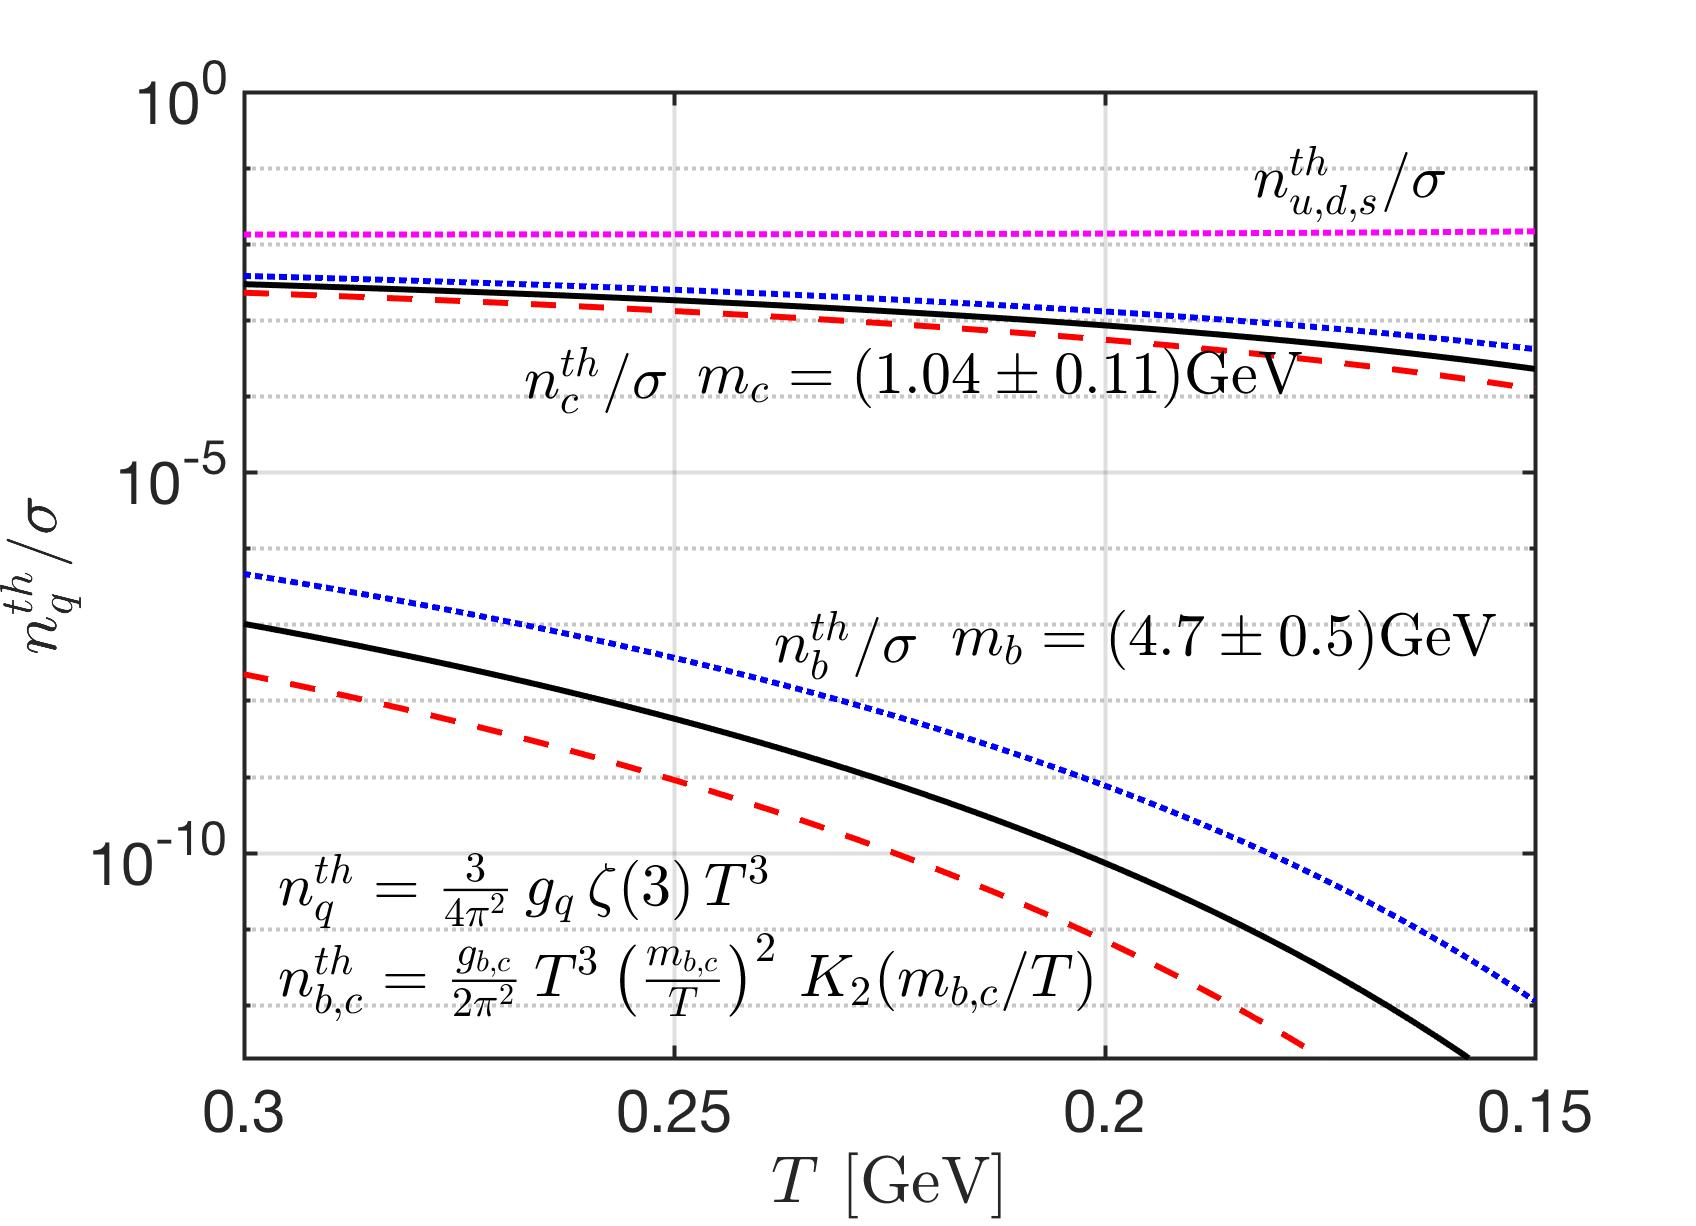
\includegraphics[width=0.9\linewidth]{./plots/bcQuarkDensity_new}}
\caption{
The equilibrium charm and bottom quark number density normalized by entropy density, as a function of temperature in the primordial Universe, see text for discussion of different mass values. \radapt{Yang:2024ret}}
\label{number_entropy_b002} 
\end{figure}
%%%%%%%%%%%%%%%%%%%%%%%%%%%%%%%%%%%%%%%%%%% 

The $m_b\simeq 5.2\,\mathrm{GeV}$ is a typical potential model mass used in modeling bound states of bottom, and $m_b=4.2,\,4.7\,\mathrm{GeV}$ is the current quark mass at low and high energy scales. In~\rf{number_entropy_b002} we see that the charm abundance in the domain of interest $0.3\,\mathrm{GeV}>T>0.15\,\mathrm{GeV}$ is about $10^4\sim 10^{9}$ times greater than the abundance of bottom quarks. This implies that the small $b$,$\bar b$ quark abundance is embedded in a large background comprising all lighter $u,d,s,c$ quarks and anti-quarks, as well as gluons $g$.

In the following we will calculate the production and decay rate for bottom and charm quarks and compare to the Universe expansion rate. We will show that in the epoch of interest to us the characteristic Universe expansion time $1/H$ is much longer than the lifespan and production time of the bottom/charm quark. In this case, the dilution of bottom/charm quark due to the Universe expansion is slow compare to the the strong interaction production, and the weak interaction decay of the bottom/charm. Any abundance nonequilibrium will therefore be nearly stationary.    

It is important for following analysis to know that the expansion of the Universe is the slowest process, allowing many microscopic reactions at a `fixed' temperature range $T$ to proceed. To show this we evaluate the Hubble relation to obtain $1/H$\,[s]
\begin{align}
H^2=\frac{8\pi G_N}{3}\left(\rho_\gamma+\rho_{\mathrm{lepton}}+\rho_{\mathrm{quark}}+\rho_{g,{W^\pm},{Z^0}}\right),
\end{align}
The effectively massless particles and radiation dominate particle energy density $\rho_i$ defining the speed of expansion of the Universe within  temperature range $130\, \mathrm{GeV}>T>0.15\,\mathrm{GeV}$; we have the following particles: photons, $8$ color charge gluons, $W^\pm$, $Z^0$, three generations of $3$ color charge quarks and leptons in the primordial QGP. The characteristic Universe expansion time constant $1/H$ is seen in~\rf{BCreaction:fig} below. In the epoch of interest to us $0.3\,\mathrm{GeV}>T>0.15\,\mathrm{GeV}$, the Hubble time $1/H\approx10^{-5}$ sec which is much longer than the microscopic lifespan and production time of the bottom and charm quarks we study 

%%%%%%%%%%%%%%%%%%%%%%%%%%%%%%%%%%%%%
\para{Quark production rate via strong interaction}\index{quark!production rate}
In primordial QGP, the bottom and charm quarks can be produced from strong interactions via quark-gluon pair fusion processes. For production, we have the following processes
\begin{align}
 q+\bar{q}&\longrightarrow b+\bar b,\qquad q+\bar{q}\longrightarrow c+\bar c,\\
 g+g&\longrightarrow b+\bar b,\qquad g+g\longrightarrow c+\bar c\,.
\end{align}

For the quark-gluon pair fusion processes\index{bottom quark!production rate}
%\begin{align}
% q+q&\longrightarrow b+\bar b,\qquad q+q\longrightarrow c+\bar c,\\
% g+g&\longrightarrow b+\bar b,\qquad g+g\longrightarrow c+\bar c,
%\end{align}
the evaluation of the lowest-order Feynman diagrams yields the cross sections~\cite{Letessier:2002ony}:
\begin{align}
&\sigma_{q\bar{q}\rightarrow b\bar{b},c\bar{c}}=\frac{8\pi\alpha_s^2}{27s}\left(1+\frac{2m_{b,c}^2}{s}\right)w(s),\,\qquad w(s)=\sqrt{1-{4m^2_{b,c}}/{s}},\\
&\sigma_{gg\rightarrow b\bar{b},c\bar{c}}=\!\frac{\pi\alpha_s^2}{3s}\bigg[\left(1\!+\!\frac{4m^2_{b,c}}{s}\!+\!\frac{m^4_{b,c}}{s^2}\right)\ln{\left(\frac{1+w(s)}{1-w(s)}\right)}\!-\!\left(\frac{7}{4}\!+\!\frac{31m^2_{b,c}}{4s}\right)w(s)\bigg],
\end{align} 
where $m_{b,c}$ represents the mass of bottom or charm quark, $s$ is the Mandelstam variable, and $\alpha_s$ is the QCD coupling constant. Considering the perturbation expansion of the coupling constant $\alpha_s$ for the two-loop approximation~\cite{Letessier:2002ony}, we have:
\begin{align}
\alpha_s(\mu^2)=\frac{4\pi}{\beta_0\ln({\mu^2/\Lambda^2})}\bigg[1-\frac{\beta_1}{\beta_0}\frac{\ln(\ln{(\mu^2/\Lambda^2)})}{\ln(\mu^2/\Lambda^2)}\bigg],
\end{align}
where $\mu$ is the renormalization energy scale and $\Lambda^2$ is a parameter that determines the strength of the interaction at a given energy scale in QCD. The energy scale we consider is based on required gluon/quark collisions above $b\bar b$ energy threshold, so we have $\mu=2m_b+T$. For the energy scale $\mu>2m_b$ we have $\Lambda=180\sim230\MeV$ ($\Lambda\approx205\MeV$ in our calculation), and the parameters $\beta_0=11-2n_f/3$, $\beta_1=102-38n_f/3$ with the number of active fermions $n_f=4$. 

%%%%%%%%%%%%%%%%%%%%%%%%%%%%%%%%%%%%%%%
\begin{figure} 
\centerline{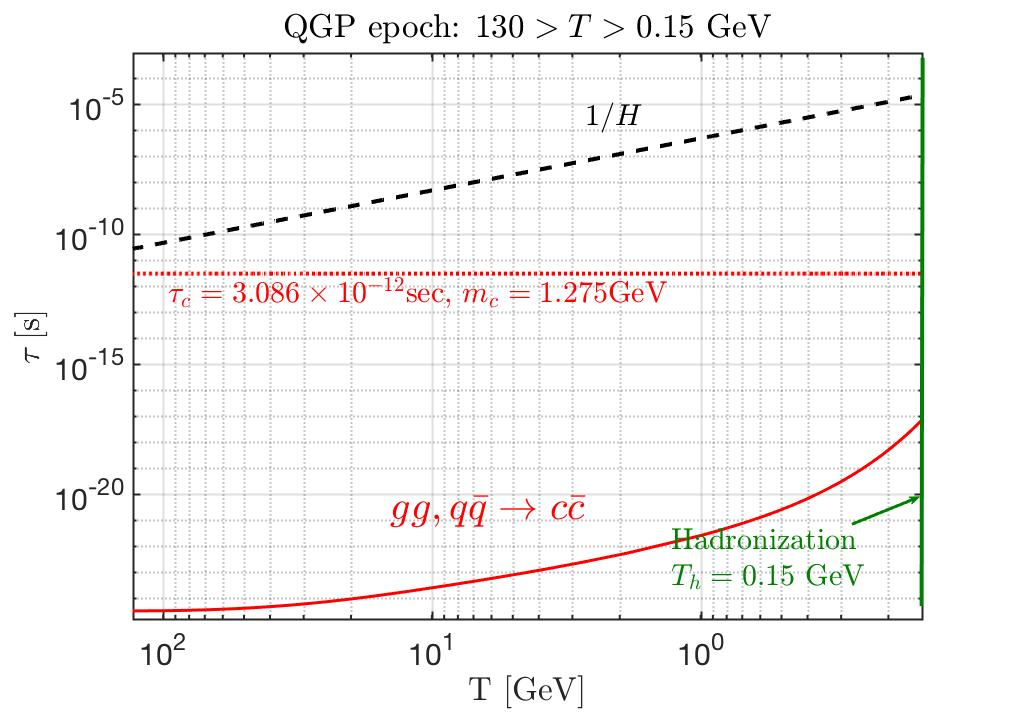
\includegraphics[width=0.9\linewidth]{./plots/CharmQuark_QGP.jpg}}
\centerline{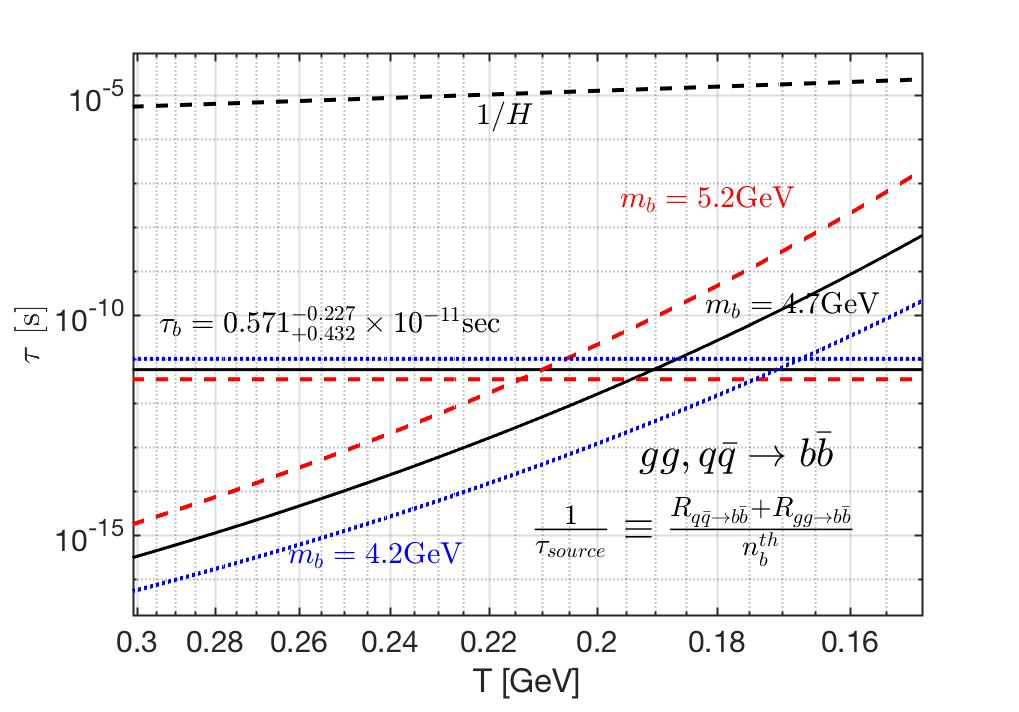
\includegraphics[width=0.9\linewidth]{./plots/BQuarkReactionTime_bottom.jpg}}
\caption{Comparison of Hubble time $1/H$, quark lifespan $\tau_{q}$, and characteristic time for production via quark, gluon pair fusion. The upper frame for charm $c$-quark in the entire QGP epoch $T$ rang; the lower frame for bottom $b$-quark amplifying the dynamic detail balance $T\simeq 200\MeV$. Both figures end at the hadronization temperature of $T_{H}\approx150\MeV$. See text for additional information. \cccite{Rafelski:2023emw}. \radapt{Yang:2024ret}}
\label{BCreaction:fig}
\end{figure}
%%%%%%%%%%%%%%%%%%%%%%%%%%%%%%%%%%%%%%%

In general the thermal reaction rate per unit time and volume $R$ can be written in terms of the scattering cross section as follows~\cite{Letessier:2002ony}:
\begin{align}
R\equiv\sum_i\int_{s_{th}}^\infty\!ds\,\frac{dR_i}{ds}=\sum_i\int_{s_{th}}^\infty\!ds\,\sigma_i(s)\,P_i(s),
\end{align}
where $\sigma_i(s)$ is the cross section of the reaction channel $i$, and $P_i(s)$ is the number of collisions per unit time and volume. Considering the quantum nature of the colliding particles (i.e., Fermi and Bose distribution) with the massless limit and chemical equilibrium condition ($\Upsilon=1$), we obtain~\cite{Letessier:2002ony}
\begin{align}
&P_i(s)=\frac{g_1g_2}{32\pi^4}\,\frac{T}{1+I_{12}}\frac{\lambda_2}{\sqrt{s}}\!\sum_{l,n=1}^{\infty}\!(\pm)^{l+n}\frac{K_1(\sqrt{lns}/T)}{\sqrt{ln}},\\
&\lambda_2\equiv\left[s-\left(m_1+m_2\right)^2\right]\,\left[s-\left(m_1-m_2\right)^2\right],
\end{align}
where $+$ is for boson and $-$ is for fermions, and the factor $1/(1+I_{12})$ is introduced to avoid double counting of indistinguishable pairs of particles. $I_{12}=1$ for identical pair of particles, otherwise $I_{12}=0$. Hence the total thermal reaction rate per volume for bottom quark production can be written as
\begin{align}
\label{Bquark_Source}
R^{\mathrm{Source}}_{b,c}=\int^\infty_{s_{th}}ds\,\bigg[\sigma_{q\bar{q}\rightarrow b\bar{b},c\bar{c}}\,P_q+\sigma_{gg\rightarrow b\bar{b},c\bar{c}}\,P_g\bigg]%=R_{q\bar{q}\rightarrow b\bar{b},c\bar{c}}+R_{gg\rightarrow b\bar{b},c\bar{c}}.
\end{align}
We introduce the bottom/charm quark relaxation time for the quark-gluon pair fusion as follows:
\begin{align}
\label{relaxation_time}
&{\tau_{b,c}^{\mathrm{Source}}}\equiv\frac{dn_{b,c}/d\Upsilon_{b,c}}{R^{\mathrm{Source}}_{b,c}}\;,\quad
\end{align}
where $dn_{b,c}/d\Upsilon_{b,c}=n^{th}_{b,c}$ in the Boltzmann approximation. The relaxation time is on the order of magnitude of time needed to reach chemical equilibrium. 

In~\rf{BCreaction:fig} we show the characteristic time for $b$ and $c$ quark strong interaction production. The $c$ quark (upper frame) is shown in the entire QGP temperature range. We note the vast 15 orders of magnitude difference between the Hubble time and the rate of production. This means that there will be very many microscopic cycles of charm production decay erasing any non-stationary effect.  For $b$ (lower frame) we restrict the view to temperature range in the domain of interest, $ 0.3\,\mathrm{GeV}>T> 0.15\,\mathrm{GeV}$. Three different masses $m_{b}=4.2\GeV$ (blue short dashes), $4.7\GeV$, (solid black), $5.2\GeV$ (red long dashes) for bottom quarks are shown. 
 
%%%%%%%%%%%%%%%%%%%%%%%%%%%%%%%%
\para{Quark decay rate via weak interaction}\index{quark!weak decay rate}
The bottom/charm quark decay via the weak interaction \index{bottom quark!decay rate} 
\begin{align}
 &b\longrightarrow c+l+\overline{\nu_l}, \qquad b\longrightarrow c+q+\bar{q},\\
&c\longrightarrow s+l+\overline{\nu_l},\qquad c\longrightarrow s+q+\bar{q}\,.
\end{align}

%\begin{align}
% &b\longrightarrow c+l+\nu_l, \qquad %b\longrightarrow c+q+\bar{q},\\
%&c\longrightarrow s+l+\nu_l,\qquad c\longrightarrow s+q+\bar{q},
%\end{align}
The vacuum decay rate for $1\to2+3+4$ in vacuum can be evaluated via the weak interaction:
\begin{align}
\frac{1}{\tau_1}=&\frac{64G^2_F\,V^2_{12}\,V^2_{34}}{(4\pi)^3g_1}\,m^5_1\times\left[\frac{1}{2}{\left(1-\frac{m^2_2}{m^2_1}-\frac{m^2_3}{m^2_1}+\frac{m^2_4}{m^2_1}\right)}\mathcal{J}_1-\frac{2}{3}\mathcal{J}_2\right],
\end{align}
where the Fermi constant is $G_F=1.166\times10^{-5}\,\mathrm{GeV}^{-2}$, $V_{ij}$ is the element of the Cabibbo-Kobayashi-Maskawa (CKM) matrix~\cite{Czarnecki:2004cw} for quark channel and $V_{l\nu_l}=1$ for lepton channel. The functions $\mathcal{J}_1$ and $\mathcal{J}_2$ are given by
\begin{align}
&\mathcal{J}_1\!=\!\!\!\int_0^{(1-m^2_2/m^2_1)/2}\!\!\!\!\!\!\!\!dx\left(1\!-\!2x\!-\!\frac{m^2_2}{m_1^2}\right)^{\!\!2}\left[\frac{1}{(1-2x)^2}-1\right]\\
&\mathcal{J}_2\!=\!\!\!\int_0^{(1-m^2_2/m^2_1)/2}\!\!\!\!\!\!\!\!dx\left(1\!-\!2x\!-\!\frac{m^2_2}{m_1^2}\right)^{\!\!3}\left[\frac{1}{(1-2x)^3}-1\right]
\end{align}
The modification due to the heat bath(plasma) is small because the bottom and charm mass $m_{b,c}\gg T$~\cite{Kuznetsova:2008jt}. In the temperature range we are interested in, the decay rate in the vacuum is a good approximation for our calculation. 

We show the lifespan for bottom and charm quarks in~\rf{BCreaction:fig}. For charm (upper frame) the decay is always much slower compared to production. This assures that the strong interaction processes can maintain equilibrium easily. Thus during the entire era of QGP charm quarks can be assumed to be in equilibrium condition. 

After hadronization, charm quarks form heavy mesons that decay into several hadronic particles. The daughter particles from charm meson decay can interact and reequilibrate within the hadron plasma. There are very many branching reactions and some involve production of only light particles. In this case the energy required to drive inverse reaction to produce heavy charm mesons is difficult to overcome. We believe this is causing the charm quark to vanish from the inventory shortly after hadronization but a detailed study has not been carried out due to complexity of the situation. 

Looking at the lower frame in~\rf{BCreaction:fig} we see that  in the case of bottom quarks the decay crosses the production rate, and this happens within QGP near to $T=200\MeV$. The intersection implies that the bottom quark freeze-out from the primordial plasma before hadronization as the production process slows down at low temperatures and the subsequent weak interaction decay leads to a dilution of the bottom quark content within the QGP plasma. All of this occurs with rates significantly faster than Hubble expansion and thus as the Universe expands, the system departs from  chemical equilibrium in near stationary manner, because of the competition between decay and production reactions in QGP. We will show how the dynamic equation cause  the distribution to deviate from equilibrium with $\Upsilon\neq1$ in the temperature range below the crossing point but before the hadronization. 

%%%%%%%%%%%%%%%%%%%%%%%%%%%%
\subsection{Is baryongenesis possible in QGP phase?}\label{Bottom}
%%%%%%%%%%%%%%%%%%%%%%%%%%%%%%%%%%%%%%%%%%%%
\index{quark!bottom nonequilibrium}
\para{Bottom quark abundance nonequilibrium}
The competition between weak interaction decay and strong interaction production rates can lead to a nonequilibrium dynamic heavy quark abundance. We explore as example the case of bottom quarks in QGP. Similar considerations apply to all heavier PP-SM particles including in particular Higgs, W,Z gauge bosons, top $t$ quark. However, the case of $b$-quarks attracted our attention early on in context of baryogenesis since there is strong known CP violation also present.
 
The dynamic equation for bottom quark abundance in QGP can be written as \index{bottom quark!population equation}
\begin{align}
\label{Bquark_eq}
\frac{1}{V}\frac{dN_b}{dt}=\big(\,1-\Upsilon^2_{b}\,\big)\,R^{\mathrm{Source}}_{b}-\Upsilon_b\,R^{\mathrm{Decay}}_{b}\;,
\end{align}
where $R^{\mathrm{Source}}_{b}$ and $R^{\mathrm{Decay}}_{b}$ are the thermal reaction rates per volume of production and decay of bottom quark, respectively. The bottom source rates are the gluon and quark fusion rates \req{Bquark_Source}. The decay rate depends on whether the bottom quarks are freely present in the plasma or are bounded within mesons. We consider two extreme scenarios for the bottom quark population: 1.) all bottom flavor is free, and 2.) all bottom flavor is bounded into mesons in QGP. In~\rf{ReactionTime} we show the characteristic interaction times relevant to the abundance of bottom quarks, as well as the Hubble time $1/H$ for the temperature range of interest, $0.3\,\mathrm{GeV}> T> 0.15\,\mathrm{GeV}$.

%%%%%%%%%%%%%%%%%%%%%%%%%%%%%%%%%%%%%%
\begin{figure} 
\centerline{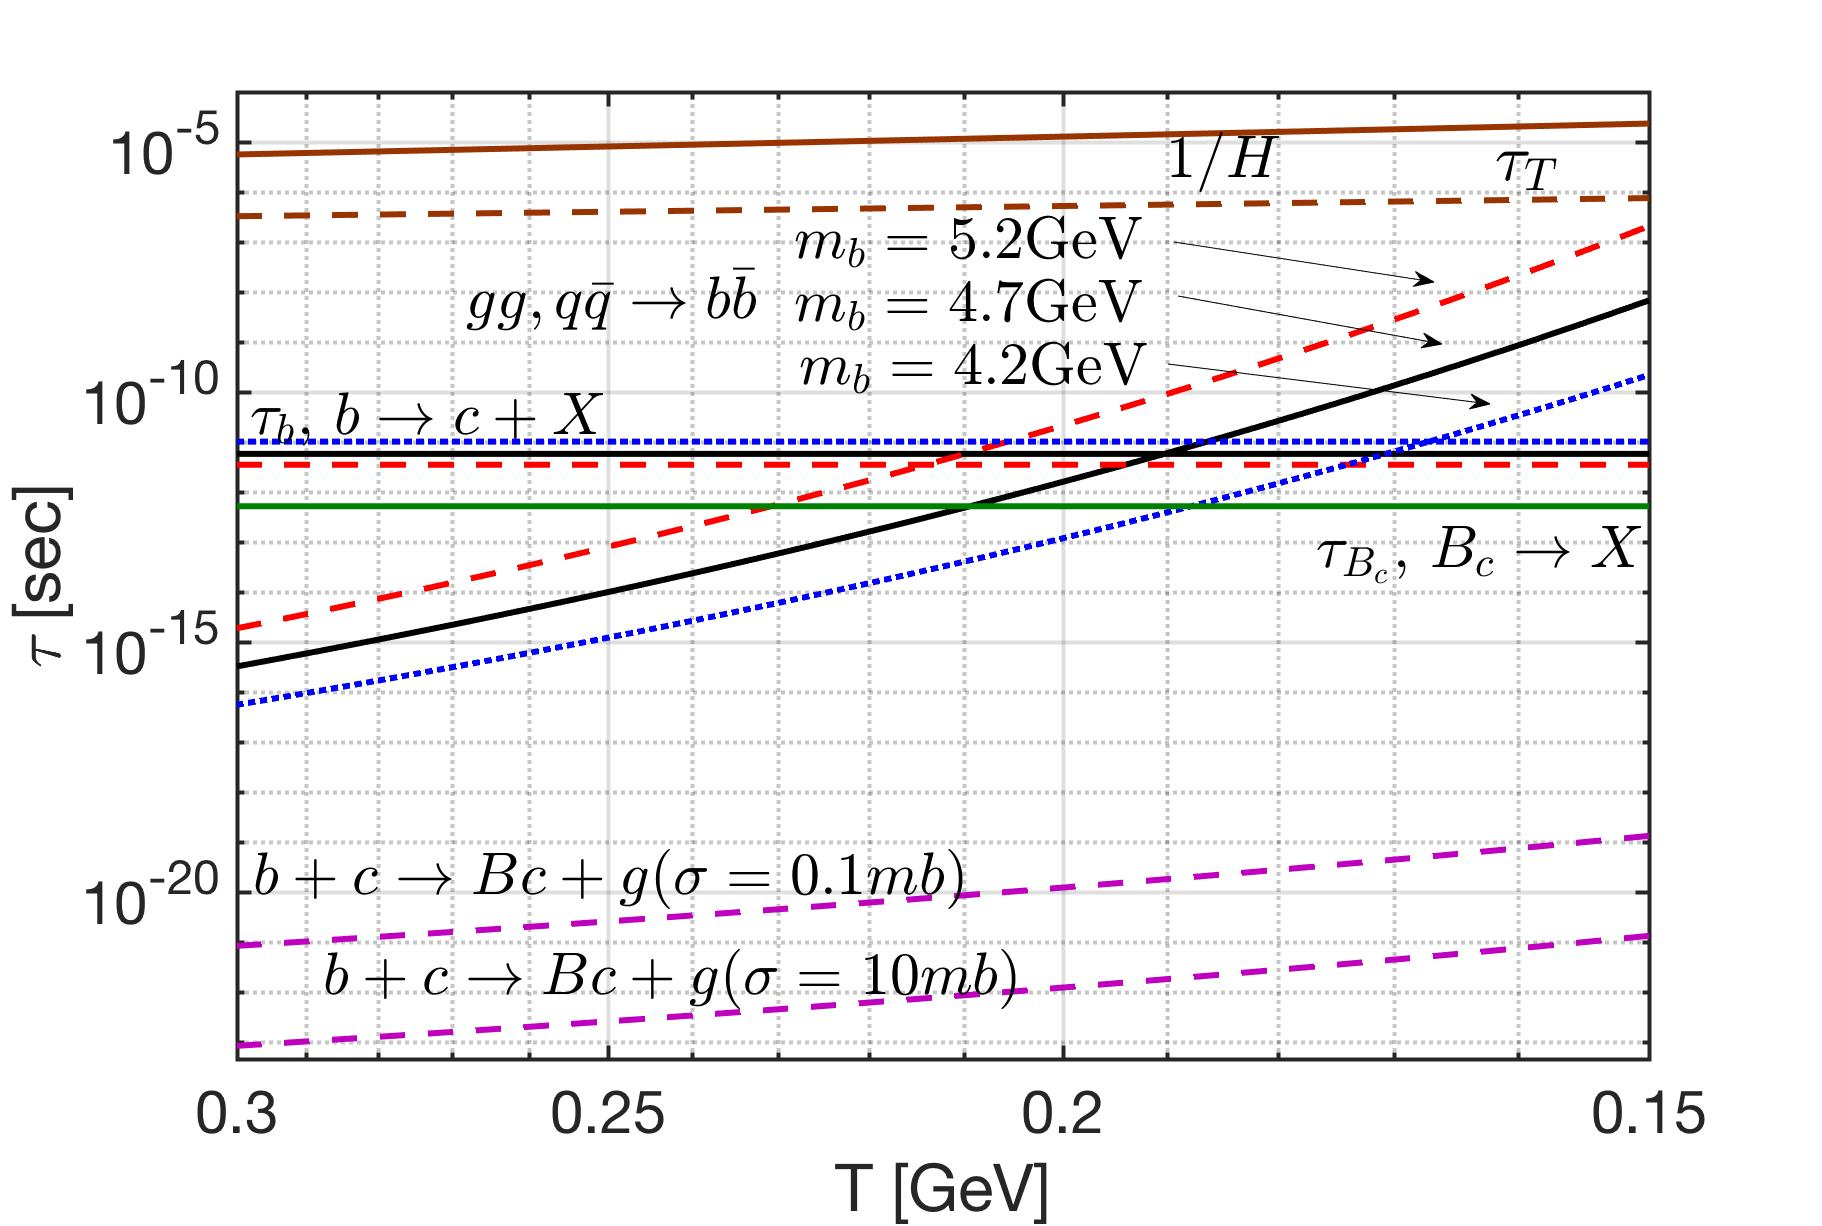
\includegraphics[width=0.9\linewidth]{./plots/BQuarkReactionTime003}}
\caption{Characteristic production, decay, times of bottom quark as a function of temperature $T$ for $0.3\,\mathrm{GeV}>T> 0.15\MeV$. Near the top of figure $1/H$ (brown solid line) and $\tau_T$ (brown dashed line); other horizontal lines are bottom-quark (in QGP) weak interaction lifetimes $\tau_b$ for the three different masses: $m_b=4.2\,\mathrm{GeV}$ (blue dotted line), $m_b=4.7\,\mathrm{GeV}$ (black solid line), $m_b=5.2\,\mathrm{GeV}$ (red dashed line), and the vacuum lifespan $\tau_B$ of the B$_c$ meson (green solid line). The relaxation time for strong interaction bottom production $g+g, q+\bar q\rightarrow b+\bar{b}$ is shown with three different bottom masses and same type-color coding as weak interaction decay rate. At bottom of figure the in plasma formation process (dashed lines, purple) $b+c\rightarrow \mathrm{B}_c+g$ with cross section range $\sigma=0.1,10\,\mathrm{mb}$. \radapt{Yang:2024ret}}
\label{ReactionTime}
\end{figure}
%%%%%%%%%%%%%%%%%%%%%%%%%%%%%%%%%

Considering all bottom flavor is free in QGP, the bottom decay rate per volume is the bottom lifespan weighted with density of particles \req{BoltzN}, see Ref.\,\cite{Kuznetsova:2008jt}. We have
\begin{align}\hspace{0.5cm}
R^{\mathrm{Decay}}_b=\frac{dn_b/d\Upsilon_b}{\tau_b},\,\,\,\,\, \tau_b\approx0.57\times10^{-11} \mathrm{sec}.
\end{align}
On the other hand, $b$,\,$\bar b$ quark abundance is embedded in a large background comprising all lighter quarks and antiquarks (see~\rf{number_entropy_b002}). After formation the heavy $b,\,\bar b$ quark can bind with any of the available lighter quarks, with the most likely outcome being a chain of reactions 
\begin{align}
&b+q\longrightarrow\mathrm{B}+g\;,\\
&\mathrm{B}+s\longrightarrow\mathrm{B}_s+q\;,\\
&\mathrm{B}_s+c\longrightarrow\mathrm{B}_c+s\;,
\end{align}
with each step providing a gain in binding energy and reduced speed due to the diminishing abundance of heavier quarks $s, c$. To capture the lower limit of the rate of $\mathrm{B}_c$ production we show in~\rf{ReactionTime} the expected formation rate by considering the direct process $b+\overline c\rightarrow \mathrm{B}_c+g$, considering the range of cross section $\sigma=0.1\sim10\,\mathrm{mb}$ ~\cite{Schroedter:2000ek}. The rapid formation rate of B$_c(b\bar c)$ states in primordial plasma is shown by purple dashed lines at bottom in~\rf{ReactionTime}, we have
\begin{align}
\tau (b+\overline c\rightarrow \mathrm{B}_c+g)\approx(10^{-16}\sim10^{-14})\times\frac{1}{H} \;.
\end{align}

Despite the low abundance of charm, the rate of $\mathrm{B}_c$ formation is relatively fast, and that of lighter flavored B-mesons is substantially higher. Note that as long as we have bottom quarks made in gluon/quark fusion bound practically immediately with any quarks $u, d, s$ into B-mesons, we can use the production rate of $b, \bar b$ pairs as the rate of B-meson formation in the primordial-QGP, which all decay with lifespan of pico-seconds. We believe that this process is fast enough to allow consideration of bottom decay from the B$_c(b\bar c)$, $\overline{\mathrm{B}}_c(\bar b c)$ states~\cite{Yang:2020nne}. 
 
Based on the hypothesis that all bottom flavor is bound rapidly into $\mathrm{B}_c^\pm$ mesons, we have 
\begin{align}\label{Bc_source}
g+g, q+q \longleftrightarrow &b+\bar b\;[b(\bar{b})+\bar{c}(c)]\longrightarrow \mathrm{B}_c^\pm\longrightarrow\mathrm{anything}.
\end{align}
In this case, the decay rate per volume can be written as
\begin{align}\hspace{0.5cm}
 R^{\mathrm{Decay}}_b=\frac{dn_b/d\Upsilon_b}{\tau_{\mathrm{B}_c}},\,\,\,\,\, \tau_{\mathrm{B}_c}\approx0.51\times10^{-12} \mathrm{sec}.
 \end{align}


%%%%%%%%%%%%%%%%%%%%%%%%%%%%%%%
\para{Stationary and non-stationary deviation from equilibrium}
To investigate the nonequilibrium phenomena of bottom quarks, we aim to replace the variation of particle abundance seen on LHS in \req{Bquark_eq} by the time variation of abundance fugacity $\Upsilon$.
This substitution allows us to derive the dynamic equation for the fugacity parameter and enables us to study the fugacity as a function of time. Considering the expansion of the Universe we have
\begin{align}\label{number_dilution}
\frac{1}{V}\frac{dN_b}{dt}=\frac{dn_b}{d\Upsilon_b}\frac{d\Upsilon_b}{dt}+\frac{dn_b}{dT}\frac{dT}{dt}+3Hn_b,\;
\end{align}
where we use $d\ln(V)/dt=3H$ for the Universe expansion. Substituting \req{number_dilution} into \req{Bquark_eq} and dividing both sides of equation by $dn_b/{d\Upsilon_b}=n^{th}_b$, the fugacity equation becomes
\begin{align}
\frac{d\Upsilon_b}{dt}+&3H\Upsilon_b+\Upsilon_b\frac{dn^{th}_b/dT}{n^{th}_b}\frac{dT}{dt}=\left(1-\Upsilon_b^2\right)\frac{1}{\tau_{b}^{\mathrm{Source}}}-\Upsilon_b\frac{1}{\tau^{\mathrm{Decay}}_b}\;,
\end{align}
where relaxation time for bottom production is obtained using \req{relaxation_time}. It is convenient to introduce the relaxation time $1/\tau_T$ as follows,
\begin{align}
\frac{1}{\tau_T}\equiv-\frac{dn^{th}_b/dT}{n^{th}_b}\frac{dT}{dt},
\end{align}
where we put '$-$' sign in the definition to have $\tau_T>0$. The relaxation time $\tau_T$ represents how the bottom density changes due to the Universe temperature cooling. In this case, the fugacity equation can be written as
\begin{align}\label{Fugacity_Eq0}
\frac{d\Upsilon_b}{dt}\!\!=&(1-\Upsilon_{b}^2)\frac{1}{\tau_{b}^{\mathrm{Source}}}
\!-\!\Upsilon_{b}\left(\frac{1}{\tau^{\mathrm{Decay}}_b}+3H\!-\!\frac{1}{\tau_T}\right).
\end{align}
In following sections we will solve the fugacity differential equation in two different scenarios: stationary and non-stationary Universe.

%%%%%%%%%%%%%%%%%%%%%%%%%%%%%%%%%%%%%%%%%%%
In~\rf{BCreaction:fig} (bottom) we show that the relaxation time for both production and decay are faster than the Hubble time $1/H$ for the duration of QGP, which implies that $H,1/\tau_T\ll1/\tau_{b}^{\mathrm{Source}},1/\tau^{\mathrm{Decay}}_b$. In this scenario, we can solve the fugacity equation by considering the stationary Universe first, i.e., the Universe is not expanding and we have
\begin{align}\label{stationary}
H=0,\qquad 1/\tau_T=0.
\end{align} 
In the stationary Universe at each given temperature we consider the dynamic equilibrium condition (detailed balance) between production and decay reactions that keep
\begin{align}
\frac{d\Upsilon_b}{dt}=0.
\end{align}
Neglecting the time dependence of the fugacity $d\Upsilon_b/dt$ and substituting the condition \req{stationary} into the fugacity equation \req{Fugacity_Eq0}, then we can solve the quadratic equation to obtain the stationary fugacity as follows: %\index{bottom quark!stationary fugacity}
\begin{align}
\label{Fugacity_Sol}
\Upsilon_{\mathrm{st}}&=\sqrt{1+\left(\frac{\tau_{source}}{2\tau_{decay}}\right)^2}-\left(\frac{\tau_{source}}{2\tau_{decay}}\right).
\end{align} 

%%%%%%%%%%%%%%%%%%%%%%%%%%%%%%%%%%%%%%
\begin{figure} 
\centerline{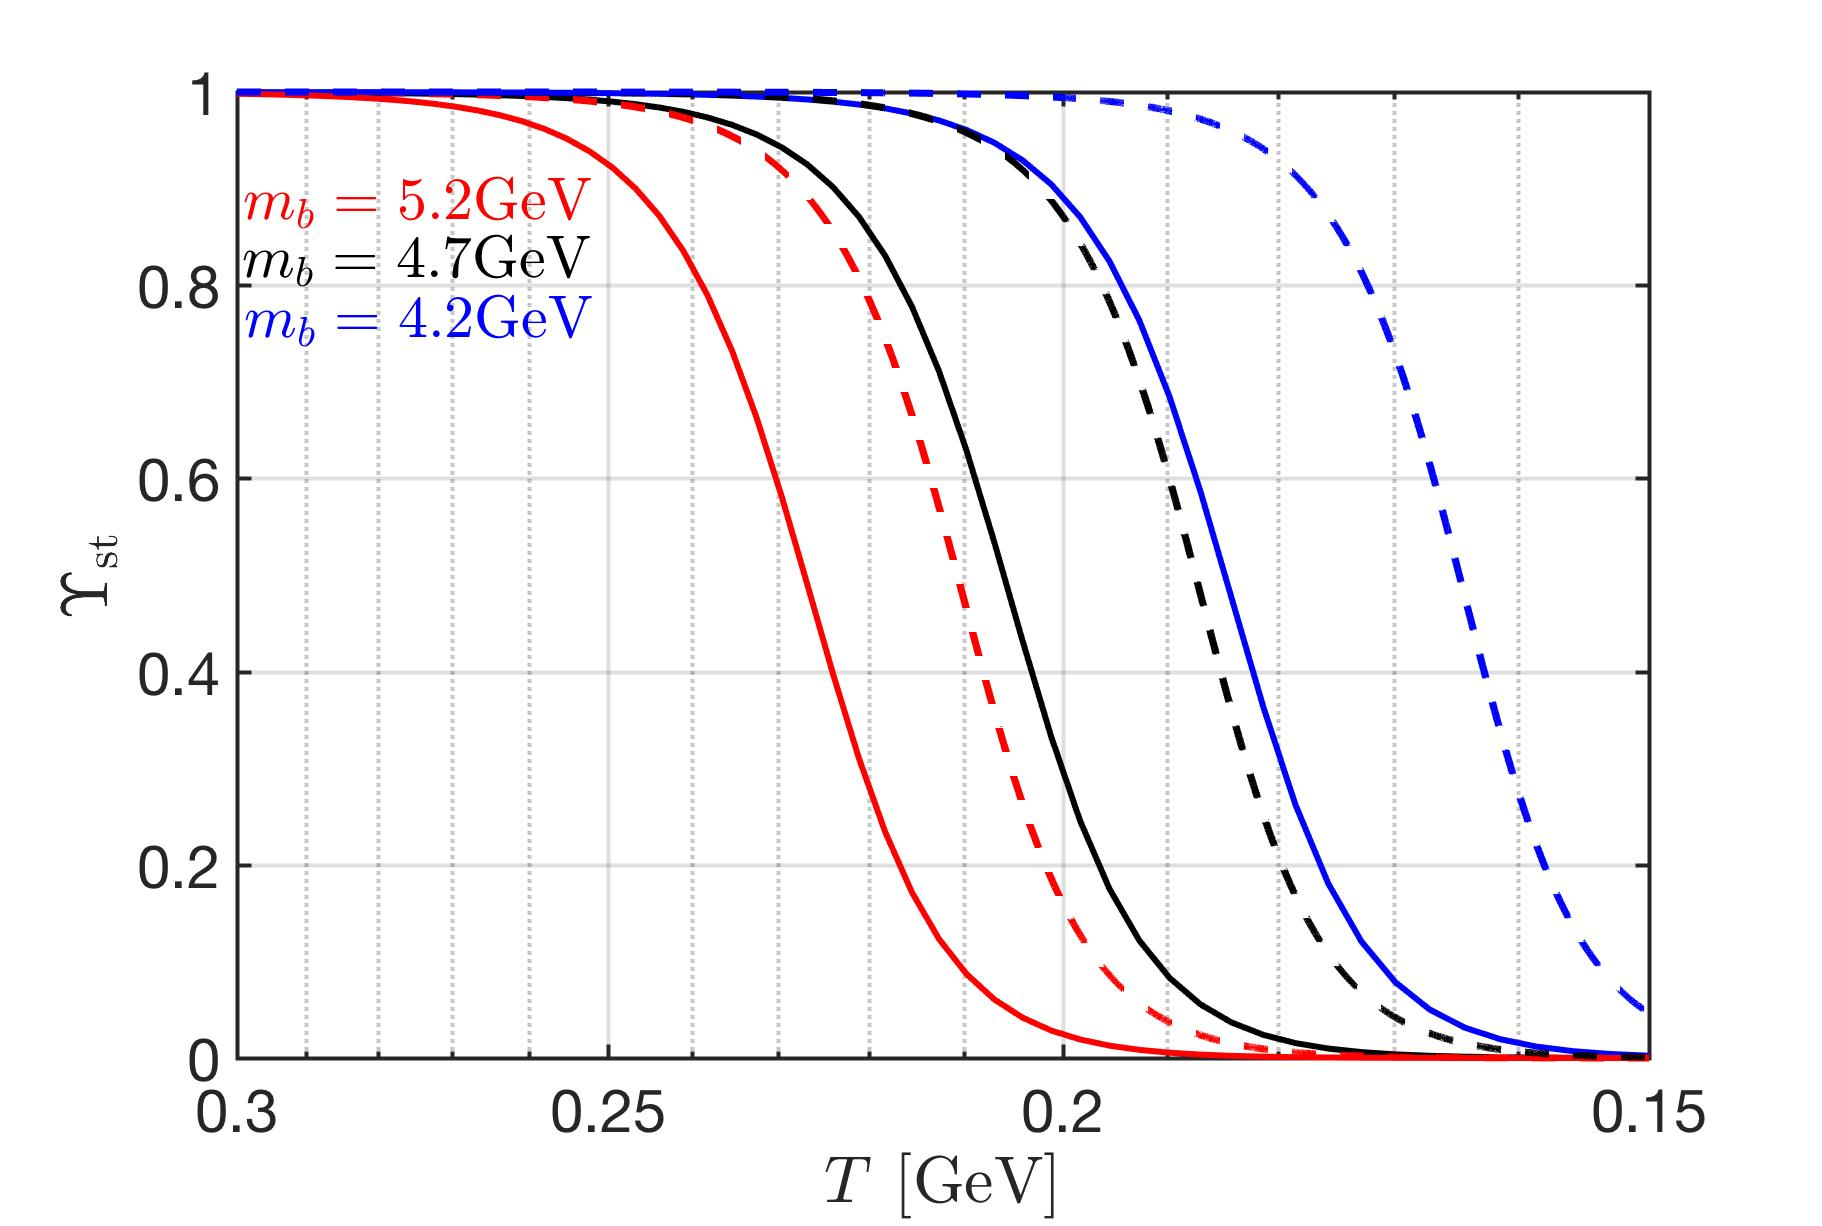
\includegraphics[width=0.9\linewidth]{./plots/BquarkFugacity_tot}}
\caption{Dynamical fugacity of bottom quark as a function of temperature in primordial Universe. Solid line shows bottom quark bound into $B_c$, dashed lines the case of free bottom quark: $m_b=4.2\,\mathrm{GeV}$ (blue), $m_b=4.7\,\mathrm{GeV}$ (black), and $m_b=5.2\,\mathrm{GeV}$ (red). \cccite{Rafelski:2023emw}. \radapt{Yang:2024ret}}
\label{fugacity_bc}
\end{figure}
%%%%%%%%%%%%%%%%%%%%%%%%%%%%%%%%%%%%%%%%%

In~\rf{fugacity_bc} the fugacity of bottom quark $\Upsilon_{\mathrm{st}}$ as a function of temperature, \req{Fugacity_Sol} is shown around the temperature $T=0.3\,\mathrm{GeV}>T>0.15\,\mathrm{GeV}$ for different masses of bottom quarks. In all cases we see prolonged nonequilibrium, this happens since the decay and reformation rates of bottom quarks are comparable to each other as we have noted in~\rf{ReactionTime} where both lines cross. One of the key results shown in~\rf{fugacity_bc} is that the smaller mass of bottom quark slows the strong interaction formation rate to the value of weak interaction decays just near the phase transformation of QGP to HG phase. Finally, the stationary fugacity corresponds to the reversible reactions in the stationary Universe. In this case, there is no arrow in time for bottom quark because of the detailed balance.

We now consider non-stationary correction in expanding Universe allowing for the Universe expanding and thus temperature being a function of time. This leads to non-stationary correction related to time dependent fugacity in the expanding Universe. 

In general, the fugacity of bottom quark can be written as 
\begin{align}\label{Nonstationary_sol}
&\Upsilon_b=\Upsilon_{\mathrm{st}}+\Upsilon^{\mathrm{non}}_{\mathrm{st}}=\Upsilon_\mathrm{st}\left(1+x\right),\quad x\equiv{\Upsilon_\mathrm{st}^{\mathrm{non}}}/{\Upsilon_\mathrm{st}},
\end{align}
where the variable $x$ corresponds to the correction due to non-stationary Universe. Substituting the general solution \req{Nonstationary_sol} into differential equation \req{Fugacity_Eq0}, we obtain
\begin{align}\label{Nonstationary_eq}
\frac{dx}{dt}=-x^2\frac{\Upsilon_\mathrm{st}}{\tau_{source}}&-x\left[\frac{1}{\tau_{eff}}+3H-\frac{1}{\tau_T}\right]-\left[\frac{d\ln\Upsilon_\mathrm{st}}{dt}+3H-\frac{1}{\tau_T}\right],
\end{align}
where the effective relaxation time $1/\tau_{eff}$ is defined as
\begin{align}
\frac{1}{\tau_{eff}}\equiv\left[\frac{2\Upsilon_\mathrm{st}}{\tau_{source}}+\frac{1}{\tau_{decay}}+\frac{d\ln\Upsilon_\mathrm{st}}{dt}\right].
\end{align}

%%%%%%%%%%%%%%%%%%%%%%%%%%%%%%
\begin{figure} 
\centerline{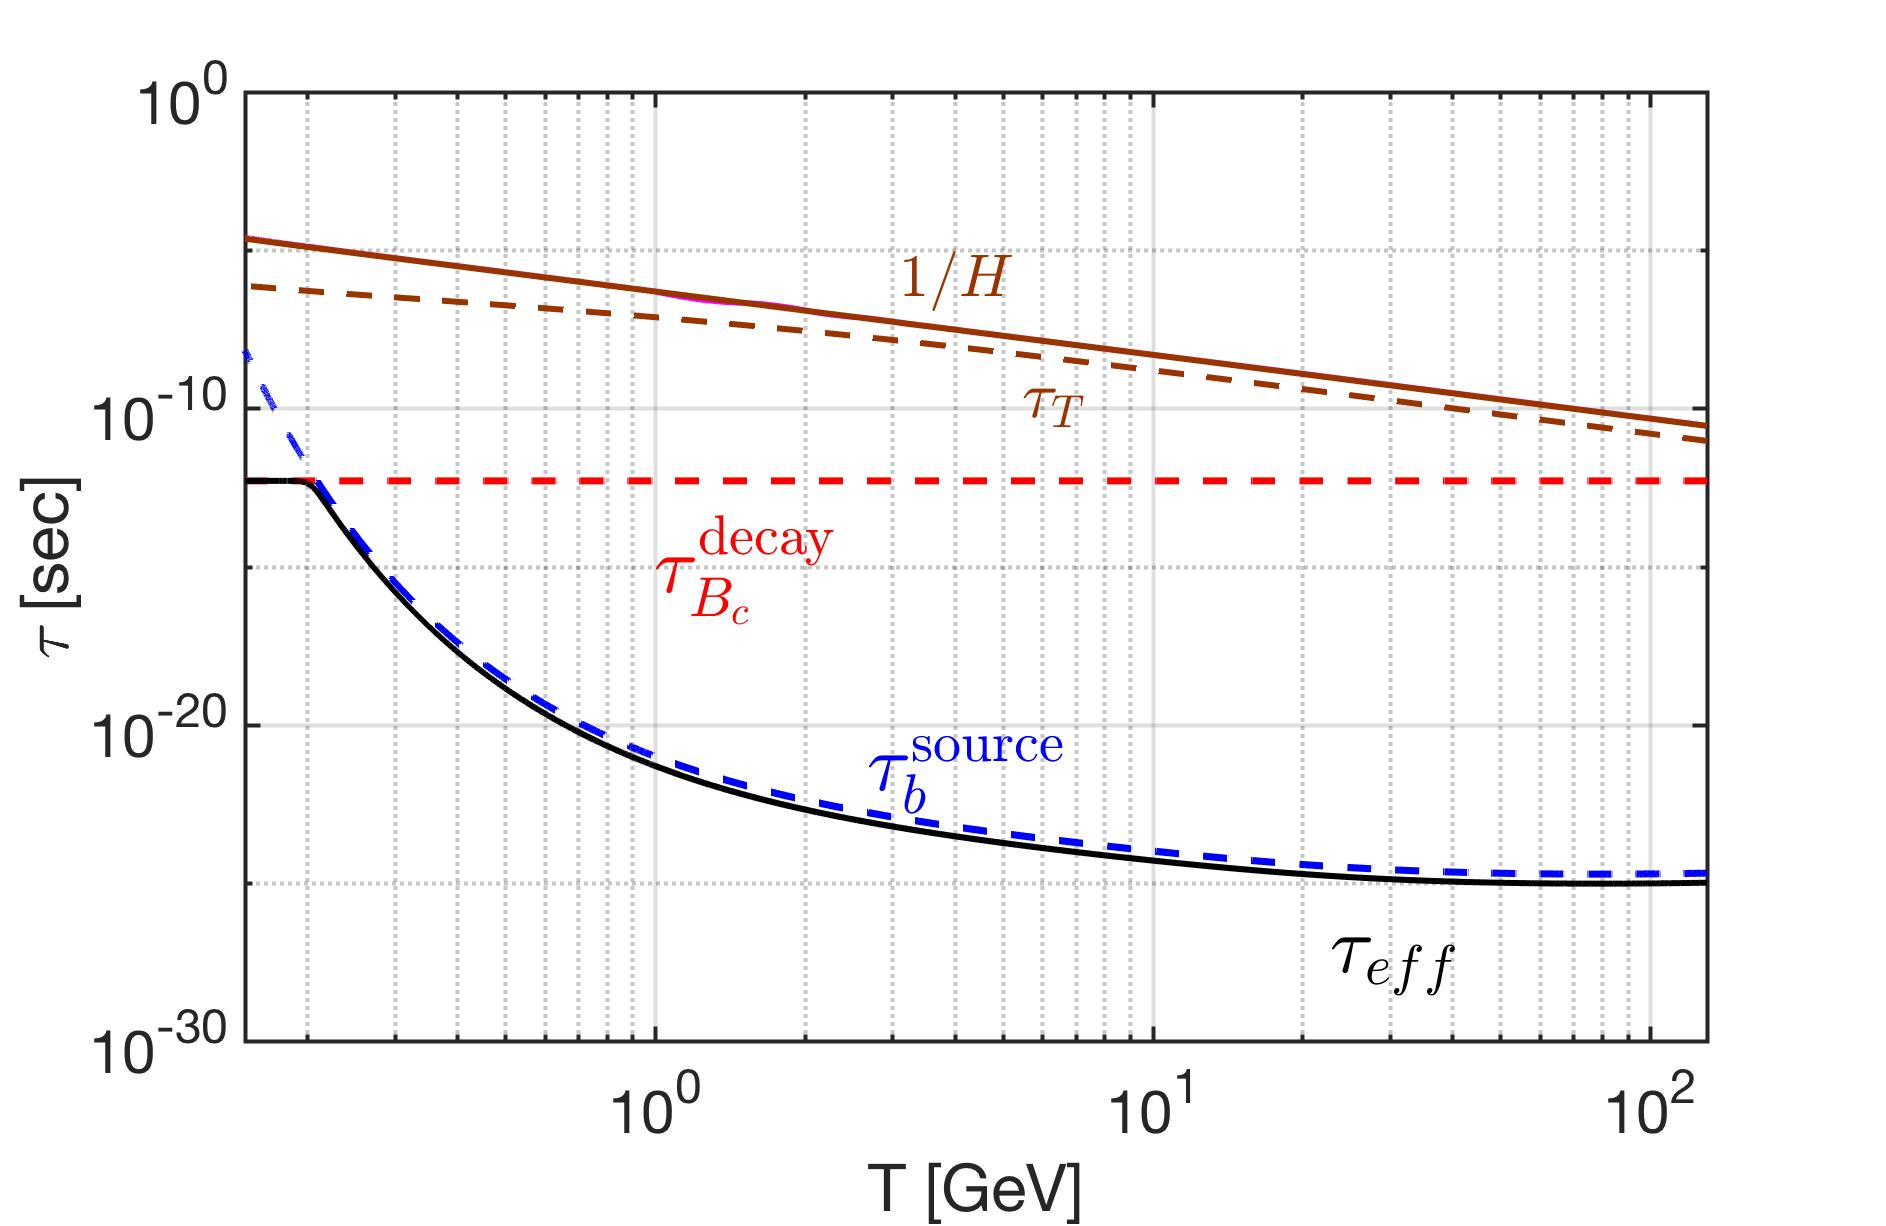
\includegraphics[width=0.9\linewidth]{./plots/Tau_RelaxationTime002}}
\caption{The effective relaxation time $\tau_{eff}$ as a function of temperature in the primordial Universe for bottom mass $m_b=4.7$\,GeV. For comparison, we also plot the vacuum lifespan of $B_c$ meson $\tau_{B_c}^{decay}$ (red dashed-line), the relaxation time for bottom production $\tau^b_{source}$ (blue dashed-line), Hubble expansion time $1/H$(brown solid line) and relaxation time for temperature cooling $\tau_T$ (brown dashed-line). \radapt{Yang:2024ret}}
\label{RelaxationTime_eff}
\end{figure}
%%%%%%%%%%%%%%%%%%%%%%%%%%%%%%%%%

In~\rf{RelaxationTime_eff} we see that when temperature is near to $T=0.2\GeV$, we have $1/\tau_{eff}\approx10^{7}H$, and $1/\tau_{eff}\approx10^5/\tau_T$. In this case, the last two terms in \req{Nonstationary_eq} compare to $1/\tau_{eff}$ can be neglected, and the differential equation becomes
\begin{align}\label{nonstationary_eq}
\frac{dx}{dt}=-\frac{x^2\,\Upsilon_\mathrm{st}}{\tau_{source}}&-\frac{x}{\tau_{eff}}-\left[\frac{d\ln\Upsilon_\mathrm{st}}{dt}+3H-\frac{1}{\tau_T}\right],
\end{align}

To solve the variable $x$ we consider the case $dx/dt,x^2\ll1$ first, we neglect the terms $dx/dt$ and $x^2$ in \req{nonstationary_eq} then solve the linear fugacity equation. We will establish that these approximations are justified by checking the magnitude of the solution. Neglecting terms $dx/dt$ and $x^2$ in \req{nonstationary_eq} we obtain
\begin{align}
x\approx\tau_{eff}\left[\frac{d\ln\Upsilon_\mathrm{st}}{dt}+3H-\frac{1}{\tau_T}\right].
\end{align}
It is convenient to change the variable from time to temperature. For an isentropically-expanding universe, we have
\begin{align}\label{tau_H}
\frac{dt}{dT}=-\frac{\tau^\ast_H}{T},\qquad \tau^\ast_H=\frac{1}{H}\left(1+\frac{T}{3g^s_\ast}\frac{dg^s_\ast}{dT}\right).
\end{align}
In this case, we have
\begin{align}
x=\tau_{eff}\left[\frac{1}{\Upsilon_\mathrm{st}}\frac{d\Upsilon_\mathrm{st}}{dT}\frac{T}{\tau^\ast_H}+3H-\frac{1}{\tau_T}\right].
\end{align}
Finally, we can obtain the non-stationary fugacity by multiplying the fugacity ratio $x$ with $\Upsilon_\mathrm{st}$, giving \index{bottom quark! non-stationary fugacity}
\begin{align}
\Upsilon_{\mathrm{st}}^{\mathrm{non}}
&\approx\left(\frac{\tau_{eff}}{\tau^\ast_H}\right)\left[\frac{d\Upsilon_\mathrm{st}}{dT}T-\Upsilon_{\mathrm{st}}\left(3H\tau^\ast_H-\frac{\tau^\ast_H}{\tau_T}\right)\right].
\end{align}

In~\rf{NonFugacity} we plot the non stationary $\Upsilon^{\mathrm{non}}_\mathrm{st}$ as a function of temperature. The non stationary fugacity $\Upsilon^{\mathrm{non}}_\mathrm{st}$ follows the behavior of $d\Upsilon_{\mathrm{st}}/dT$, which corresponds to the irreversible process in expanding Universe. In this case, the irreversible nonequilibrium process creates the arrow in time for bottom quark in the Universe. The large value of Hubble time compares to the effective relaxation time suppressing the value of non-stationary fugacity to $\mathcal{O}\sim10^{-7}$, which shows that the neglecting $dx/dt,x^2\ll1$ is a good approximation for solving the non-stationary fugacity in the primordial Universe.


%%%%%%%%%%%%%%%%%%%%%%%%%%%%%%%%%%%
\begin{figure}
\centerline{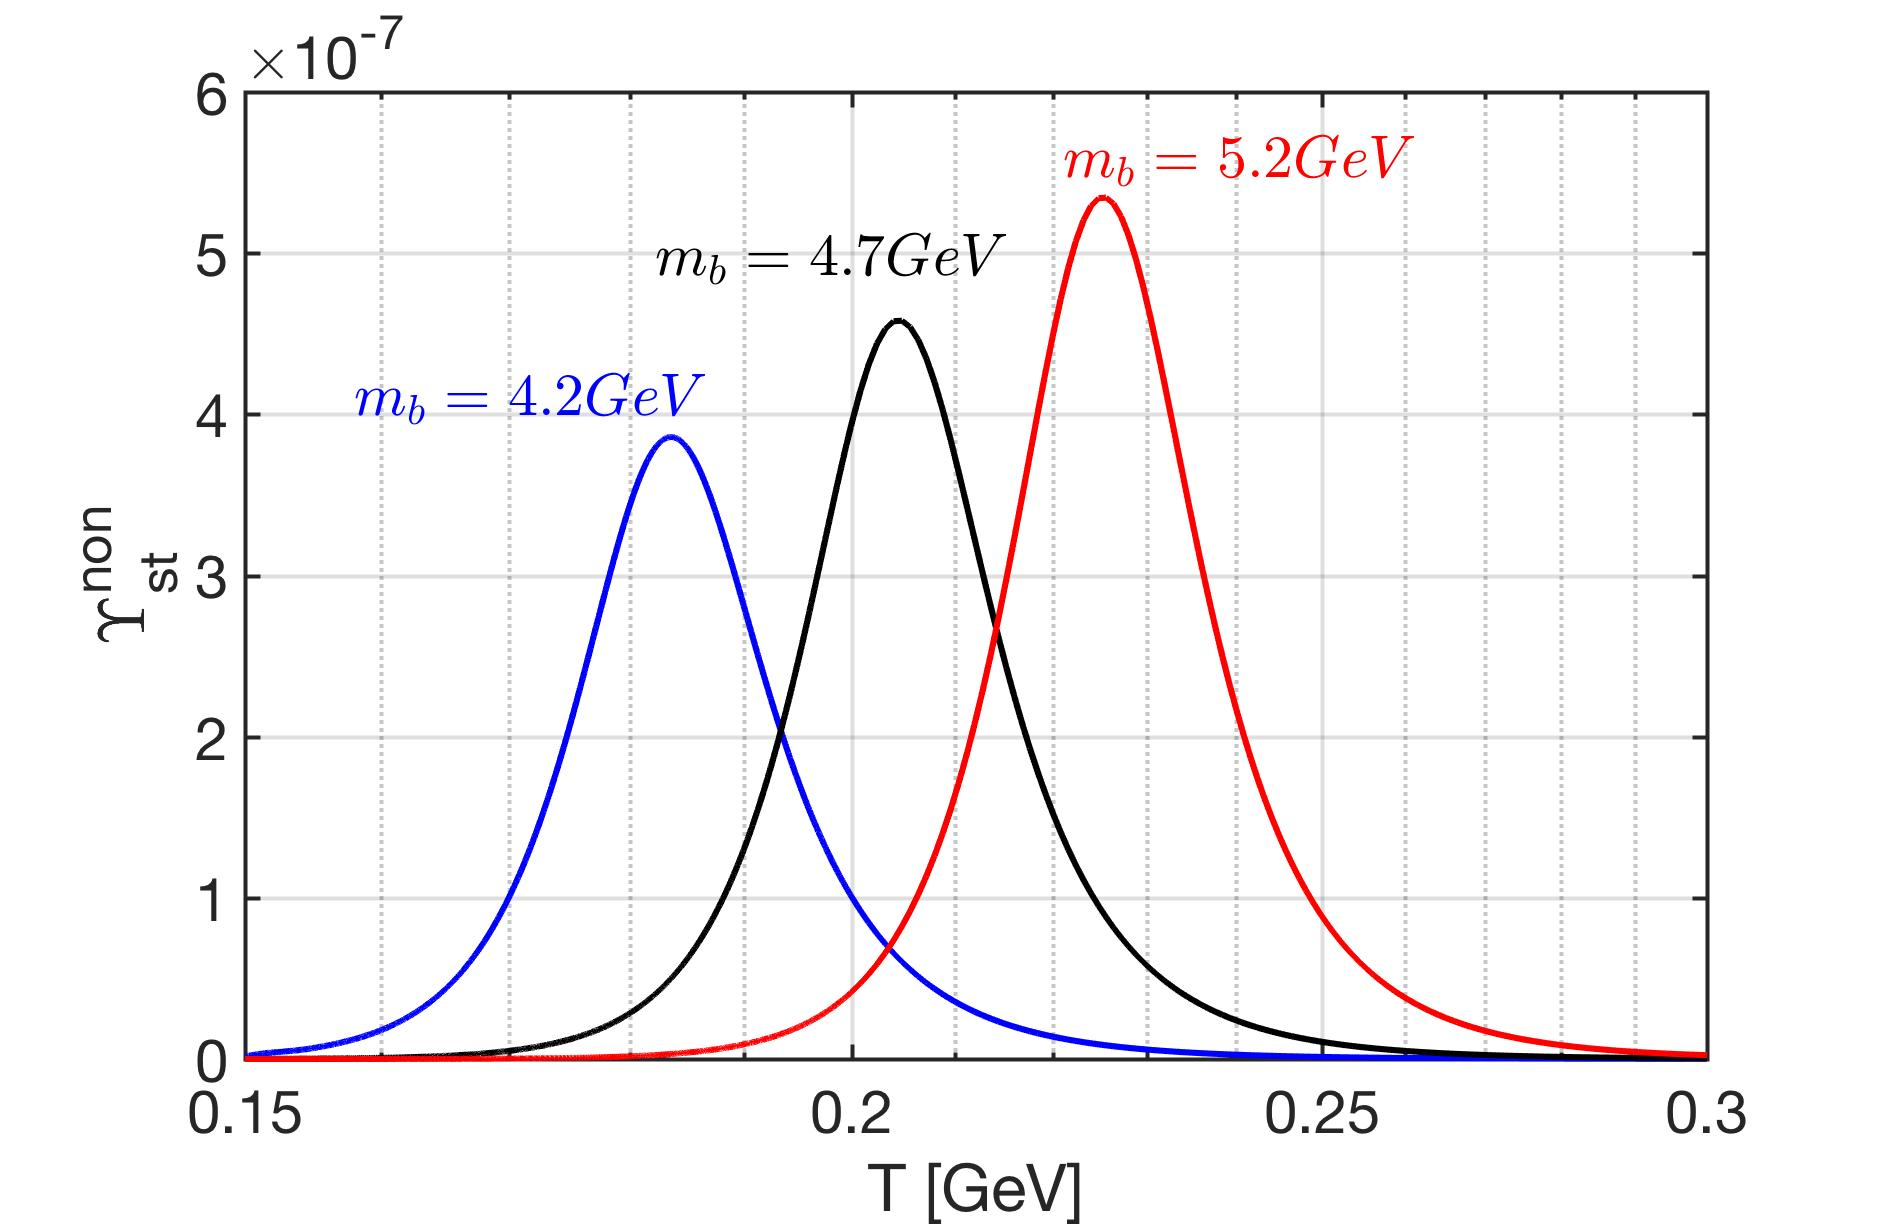
\includegraphics[width=0.9\linewidth]{./plots/NonstationaryFugacity}}
\caption{The non-stationary fugacity $\Upsilon_\mathrm{st}^{\mathrm{non}}$ as a function of temperature in the Universe for different bottom mass $m_b=4.2\,\mathrm{GeV}$ (blue), $m_b=4.7\,\mathrm{GeV}$ (black), and $m_b=5.2\,\mathrm{GeV}$ (red) for the case bottom quarks bound into $B_c$ mesons. \radapt{Yang:2024ret}}
\label{NonFugacity}
\end{figure}
%%%%%%%%%%%%%%%%%%%%%%%%%%%%%%%%%%%%%%
 

%%%%%%%%%%%%%%%%%%%%%%%%%%%%%%%%%%
\para{Is there enough bottom flavor to matter?} Considering that FLRW-Universe evolves conserving entropy, and that baryon and lepton number following on the era of matter genesis is conserved, the current day baryon $B$ to entropy $S$, $B/S$-ratio must be achieved during matter genesis. The estimates of present day baryon-to-photon density ratio $\eta$ allows the determination of the present value of baryon per entropy ratio \cite{Rafelski:2019twp,Letessier:2002ony,Fromerth:2002wb,Fromerth:2012fe}:
\begin{align}
\left(\frac{B}{S}\right)_{t_0}\!\!\!\!=\eta\left(\frac{n_\gamma}{\sigma_\gamma+\sigma_\nu}\right)_{\!t_0}\!\!\!\!=(8.69\pm0.05)\!\!\times\!\!10^{-11},
\end{align}
where the subscript $t_0$ denotes the present day value, where $\eta=(6.12\pm0.04)\times10^{-10}$~\cite{ParticleDataGroup:2018ovx} is used in calculation. Here we consider that the Universe today is dominated by photons and free-streaming low mass neutrinos~\cite{Birrell:2012gg}, and $\sigma_\gamma$ and $\sigma_\nu$ are the entropy density for photons and neutrinos, respectively. 
 
In chemical equilibrium the ratio of bottom quark (pair) density $n_b^{th}$ to entropy density $\sigma=S/V$ just above quark-gluon hadronization temperature $T_\mathrm{H}=150\sim160\MeV$ is $n_b^{th}/\sigma=10^{-10}\sim 10^{-13}$ (see~\rf{number_entropy_b002}. By studying the bottom density per entropy near to the hadronization temperature and comparing it to the baryon-per-entropy ratio $B/S$ we found that there is sufficient abundance of bottom quarks for the proposed matter genesis mechanism to be relevant.

%%%%%%%%%%%%%%%%%%%%%%%%%%%%%%%%
\para{Example of bottom-catalyzed matter genesis}
Given that the nonequilibrium non-stationary component of bottom flavor arises at relatively low QGP temperature, this Sakharov condition is available around QGP hadronization. Let us now look back and see how different requirements are fulfilled
%%%%%%%%%%%%%%%%%%%%%%%%%%%%%%%%%%%%
\begin{itemize}
\item
 We have demonstrated non-stationary conditions with absence of detailed balance: The competition between weak interaction decay and the strong interaction gluon fusion process is responsible for driving the bottom quark departure from the equilibrium in the primordial Universe near to QGP hadronization condition around the temperature $T=0.3\sim0.15\GeV$ as shown in~\rf{fugacity_bc}. Albeit small there is clear non-stationary component required for baryogenesis, see~\rf{NonFugacity}.
%%%%%%%%%%%%%%%%%%%%%%%%%%%%%%%
\item Violation of $CP$ asymmetry were observed in the amplitudes of hadron decay including neutral B-mesons, see for example~\cite{LHCb:2019jta,LHCb:2020vut}. The weak interaction $CP$ violation\index{CP!violation}\index{CKM!mtrix} arises from the components of Cabibbo-Kobayashi-Maskawa (CKM) matrix associated with quark-level transition amplitude and $CP$-violating phase. There is clear coincidence of non stationary component of bottom yield with the bottom quark $CP$ violating decays of preformed $\mathrm{B}_x$ meson states, $x=u,d,s,c$~\cite{Karsch:1987pv,Brambilla:2010vq,Aarts:2011sm,Brambilla:2017zei,Bazavov:2018wmo,Offler:2019eij}. The exploration of the here interesting $CP$ symmetry breaking in B$_c(b\bar c)$ decay is in progress~\cite{Tully:2019ltb,HFLAV:2019otj,ParticleDataGroup:2018ovx}. % Present measurements of $CP$-violation suggest that the CP asymmetry parameter is around $\delta_{CP}\approx10^{-3}$ ~\cite{ParticleDataGroup:2018ovx}.
\item
We do not know if there is baryon number violating process in which one of the heavy particles, including bottom quark, is participating. However, if such a process were to exist it is likely, considering mass thresholds, that it would be most active in the decays of heaviest standard model particles. It is thus of considerable interest to study in lepton colliders baryon number non conserving processes at resonance condition. Such a research program will additionally be motivated by our demonstration of an extended period of baryogenesis in the primordial Universe. 
\end{itemize}

%%%%%%%%%%%%%%%%%%%%


\para{Circular Urca amplification}
The off equilibrium phenomenon of bottom quark around the temperature range $T=0.3\sim0.15\GeV$ can provide the non-chemical equilibrium non-stationary condition for baryogenesis to occur in the primordial-QGP hadronization era. The processes of interest as we saw are small. However there is additional amplifying factor. 
 
 Let us consider the scenario where all bottom quarks are confined within $B_c^\pm$ meson. In this case, the decay of charged mesons in the primordial-QGP can be a source of $CP$ violation. However, it remains uncertain whether the decay of $B_c^\pm$ mesons contributes to baryon violation. Our postulation is as follows: the baryon asymmetry is produced by the bottom quark disappearance via the irreversible decay of $B^\pm_c$ meson during the off-equilibrium process. Once a baryon symmetry exists in universe, it will also produce the asymmetry between leptons and anti-leptons which is similar to the baryon asymmetry by the $L=B$.

The heavy $B_c^\pm$ meson decay into multi-particles in plasma is associated with the irreversible process. This is because after decay the daughter particles can interact with plasma and distribute their energy to other particles and reach equilibrium with the plasma quickly. In this case the energy required for the inverse reaction to produce $B_c^\pm$ meson is difficult to overcome and therefore we have an irreversible process for multi-particle decay in plasma.


The rapid $B_c^\pm$ decay and bottom reformation speed at picosecond scale assures that there are millions of individual microscopic processes involving bottom quark production and decay before and during the hadronization epoch of QGP. In this case, we have an Urca process for the bottom quark, i.e. a cycling reaction that produces the bottom quark which subsequently disappears via the $B_c^\pm$ meson decay. 

The Urca process is a fundamental physical process and has been studying the realms of in astrophysics and nuclear physics. In our case, for bottom quark as a example: at low temperature, the number of bottom quark cycling can be estimated as
\begin{align}
\left.\mathrm{C_{cycle}}\right|_{T=0.2\mathrm{GeV}}=\frac{\tau_H}{\tau_{B_c}}\approx2\times10^7,
\end{align}
where the lifespan of $B_c^\pm$ is $\tau_{\mathrm{B}_c}\approx0.51\times10^{-12}\,\mathrm{sec}$ and at temperature $T=0.2\GeV$ the Hubble time is $\tau_H=1/H=1.272\times10^{-5}$ sec. The Urca process plays a significant role by potentially amplifying any small and currently unobserved violation of baryon number associated with the bottom quark. The small baryon asymmetry is enhanced by the Urca-like process with cycling ${\tau^\ast_H}/{\tau_\ast}$ in the primordial Universe.
This amplification would be crucial for achieving the required strength for today's observation. 


%%%%%%%%%%%%%%%%%%%%%%%%%%%%%%%%%%%%%%%%%%%%%%%%
\subsection{Strange hadron abundance in cosmic plasma}
\label{Strangeness}\index{strangeness}
%%%%%%%%%%%%%%%%%%%%%%%%%%%%%%%%%%
\para{Hadron populations in equilibrium}
As the Universe expanded and cooled down to the QGP Hagedorn temperature $T_H\approx150\MeV$, the primordial QGP underwent a phase transformation called hadronization. Quarks and gluons fragmented, combined and formed matter and antimatter  we are familiar with. After hadronization, one may think that all relatively short lived massive hadrons decay rapidly and disappear from the Universe. However, the most abundant hadrons, pions $\pi(q\bar q)$, can be produced via their inverse decay process $\gamma\gamma\rightarrow\pi^0$. Therefore they retain their chemical equilibrium  down to $T=3\sim5\MeV$~\cite{Kuznetsova:2008jt}. 

We begin by determining the Universe particle population composition assuming both kinetic and particle abundance equilibrium (chemical equilibrium) of non-interacting bosons and fermions. By considering the charge neutrality and a prescribed conserved baryon-per-entropy-ratio ${(n_B-n_{\overline{B}})}/{\sigma}$ we can  determine the baryon chemical potential $\mu_B$~\cite{Fromerth:2002wb,Fromerth:2012fe,Rafelski:2013yka}. We extend this approach  allowing for the presence of strange hadrons, and imposing conservation of strangeness in the primordial Universe -- the  strange quark content in hadrons must equal the anti-strange quark content in statistical average $\langle s-\bar s \rangle=0$. 

Given $\mu_B(T)$, $\mu_s(T)$ the baryon and strangeness chemical potentials as a function of temperature, we can obtain the particle number densities for different strange and non-strange species and study their population in the primordial Universe. Our approach prioritizes strangness pair production into bound hadron states by strong or electromagnetic interactions over the also possible weak interaction strangness changing processes capable to amplify the effect of baryon asymmetry. This is another topic beyond scope of this work and deserving further attention.

To characterize the baryon and strangeness content of a hadron we employ the chemical fugacity for strangeness $\lambda_s$ and for light quarks $\lambda_q$ \index{quark!fugacity}
\begin{align}
\lambda_s=\exp(\mu_s/T)\,\quad \lambda_q=\exp(\mu_B/3T)\,.
\end{align}
Here $\mu_s$ and $\mu_B$ are the chemical potential of strangeness and baryon, respectively. To obtain quark fugacity $\lambda_q$, we divide the baryo-chemical potential of baryons by quark content in the baryon, \ie\ three.

When the baryon chemical potential does not vanish the chemical potential of strangeness in the primordial Universe is obtained imposing the conservation of strangeness constraint $\langle s-\bar s \rangle=0$, see Section 11.5 in Ref.\,\cite{Letessier:2002ony}\index{strangeness! chemical potential}
\begin{align}\label{museq}
\lambda_s=\lambda_q\sqrt{\frac{F_K+\lambda^{-3}_q\,F_Y}{F_K+\lambda^3_q\,F_Y}}\,.
\end{align}
where we employ the phase-space function $F_i$ for sets of nucleon $N$, kaons $K$, and hyperon $Y$ particles 
\begin{align}
&F_N=\sum_{N_i}\,g_{N_i}W(m_{N_i}/T)\;, \quad N_i=n, p, \Delta(1232),\\
&F_K=\sum_{K_i}\,g_{K_i}W(m_{K_i}/T)\;, \quad K_i=K^0, \overline{K^0}, K^\pm, K^\ast(892),\\
&F_Y=\sum_{Y_i}\,g_{Y_i}W(m_{Y_i}/T)\;, \quad Y_i=\Lambda, \Sigma^0,\Sigma^\pm, \Sigma(1385),
\end{align}
$g_{N_i,K_i,Y_i}$ are the degeneracy factors, $W(x)=x^2K_2(x)$ with $K_2$ is the modified Bessel functions of integer order `$2$'. 

Considering the massive particle number density in the Boltzmann approximation we obtain
\begin{align}
\label{Density_N}
&n_N=\frac{T^3}{2\pi^2}\lambda_q^3F_N,\quad\qquad\qquad n_{\overline N}=\frac{T^3}{2\pi^2}\lambda^{-3}_qF_N,\\
\label{Density_K}
&n_K=\frac{T^3}{2\pi^2}\left(\lambda_s\lambda_q^{-1}\right)F_K,\,\qquad n_{\overline{K}}=\frac{T^3}{2\pi^2}\left(\lambda_s^{-1}\lambda_q\right)F_K,\\
\label{Density_Y}
&n_Y=\frac{T^3}{2\pi^2}\left(\lambda_q^2\lambda_s\right)F_Y,\quad\qquad n_{\overline Y}=\frac{T^3}{2\pi^2}\left(\lambda^{-2}_q\lambda_s^{-1}\right)F_Y.
\end{align}
In this case, the net baryon density in the primordial Universe with temperature range $150\MeV> T>10\MeV$ can be written as 
\begin{align}
\frac{\left(n_B-n_{\overline{B}}\right)}{\sigma}&=\frac{1}{\sigma}\left[\left(n_p-n_{\overline{p}}\right)+\left(n_n-n_{\overline{n}}\right)+\left(n_Y-n_{\overline{Y}}\right)\right]\notag\\
&=\frac{T^3}{2\pi^2\,\sigma}\left[\left(\lambda_q^3-\lambda^{-3}_q\right)F_N+\left(\lambda_q^2\lambda_s-\lambda^{-2}_q\lambda_s^{-1}\right)F_Y\right]\notag\\
&=\frac{T^3}{2\pi^2\sigma}\left(\lambda_q^3-\lambda_q^{-3}\right)F_N\left[1+\frac{\lambda_s}{\lambda_q}\left(\frac{\lambda_q^3-\lambda^{-1}_q\lambda_s^{-2}}{\lambda^3_q-\lambda^{-3}_q}\right)\,\frac{F_Y}{F_N}\right]\notag\\
&\approx\frac{T^3}{2\pi^2\sigma}\left(\lambda_q^3-\lambda_q^{-3}\right)F_N\left[1+\frac{\lambda_s}{\lambda_q}\,\frac{F_Y}{F_N}\right],
\end{align}
where we can neglect the term $F_Y/F_K$ in the expansion of \req{museq} in our temperature range. 

Introducing the strangeness conservation $\langle s-\bar s\rangle=0$ constraint and using the entropy density in primordial Universe, the explicit relation for baryon to entropy ratio becomes
\begin{align}\label{muBeq}
\frac{n_B-n_{\overline{B}}}{\sigma}&=\frac{45}{2\pi^4g^s_\ast}\sinh\left[\frac{\mu_B}{T}\right]F_N\times\left[1+\frac{F_Y}{F_N}\sqrt{\frac{1+e^{-\mu_B/T}\,F_Y/F_K}{1+e^{\mu_B/T}\,F_Y/F_K}}\right].
\end{align}
The present-day baryon-per-entropy-ratio is needed  in \req{muBeq}  and we obtain the value 
\begin{align}\label{BdS}
\frac{n_B-n_{\overline{B}}}{\sigma}= \left.\frac{n_B-n_{\overline{B}}}{ \sigma}\right|_{t_0}=(0.865\pm0.008)\times10^{-10} \;.
\end{align}

For a details of evaluation method we refer to our earlier work, however we have updated results to the updated baryon-to-photon ratio~\cite{ParticleDataGroup:2018ovx}: $\left(n_B-n_{\overline{B}}\right)/n_\gamma= (0.609\pm0.06)\times10^{-9}$, supplemented by quantum value of entropy per particle for a massless boson $\sigma/n|_\mathrm{boson}\approx 3.60$, and for a massless fermion $\sigma/n|_\mathrm{fermion}\approx 4.20$. We solve \req{museq}) and \req{muBeq} numerically to obtain baryon and strangeness chemical potentials as a function of temperature shown in~\rf{ChemPotFig}.

%%%%%%%%%%%%%%%%%%%%%%%%
\begin{figure} 
\centerline{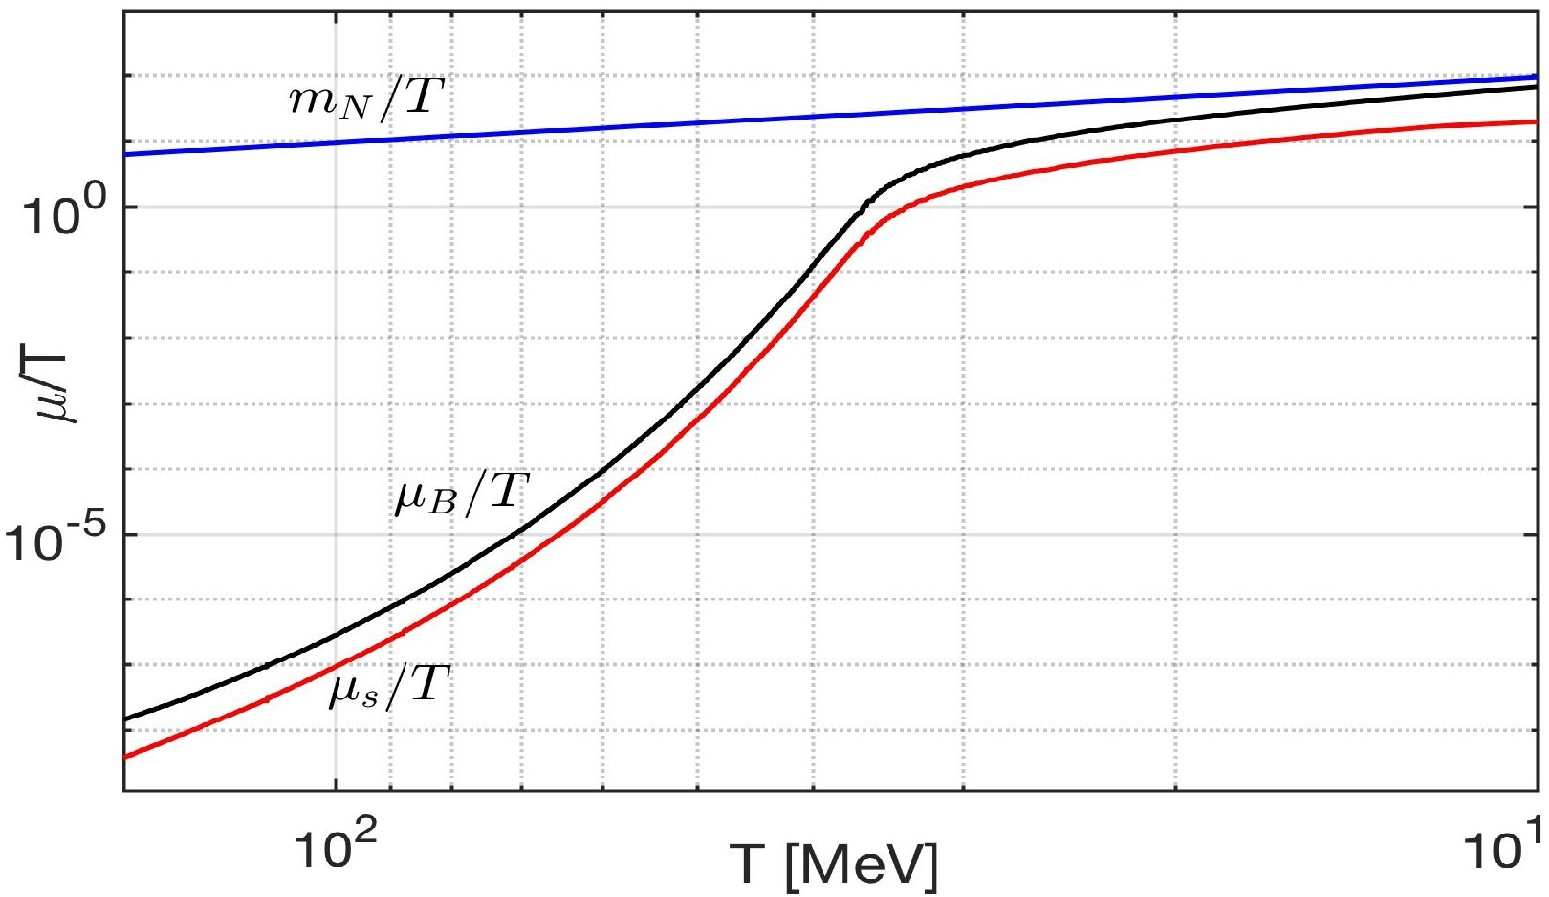
\includegraphics[width=0.9\linewidth]{./plots/New_Chemical_Potential_C.jpg}}
\caption{The chemical potential of baryon number $\mu_B/T$ and strangeness $\mu_s/T$ as a function of temperature $150\MeV> T>10\MeV$ in the primordial Universe; for comparison we show $m_N/T $ with $m_N=938.92\MeV$, the average nucleon mass. \cccite{Yang:2021bko}. \radapt{Yang:2024ret}}
\label{ChemPotFig}\index{baryon!chemical potential}\index{strangeness!chemical potential} 
\end{figure}
%%%%%%%%%%%%%%%%%%%%%%%%%%%%%%

The chemical potential in~\rf{ChemPotFig} changes dramatically in the temperature window $50\MeV\le T\le 30\MeV$, its behavior is describing the antibaryon disappearance from Universe inventory. Substituting the chemical potential $\lambda_q$ and $\lambda_s$ into particle density \req{Density_N}, \req{Density_K}, and \req{Density_Y}, we can obtain the particle number densities for different species as a function of temperature.

%%%%%%%%%%%%%%%%%%%%%%%%%%%%%%%%%%%%%%%
\begin{figure} 
\centerline{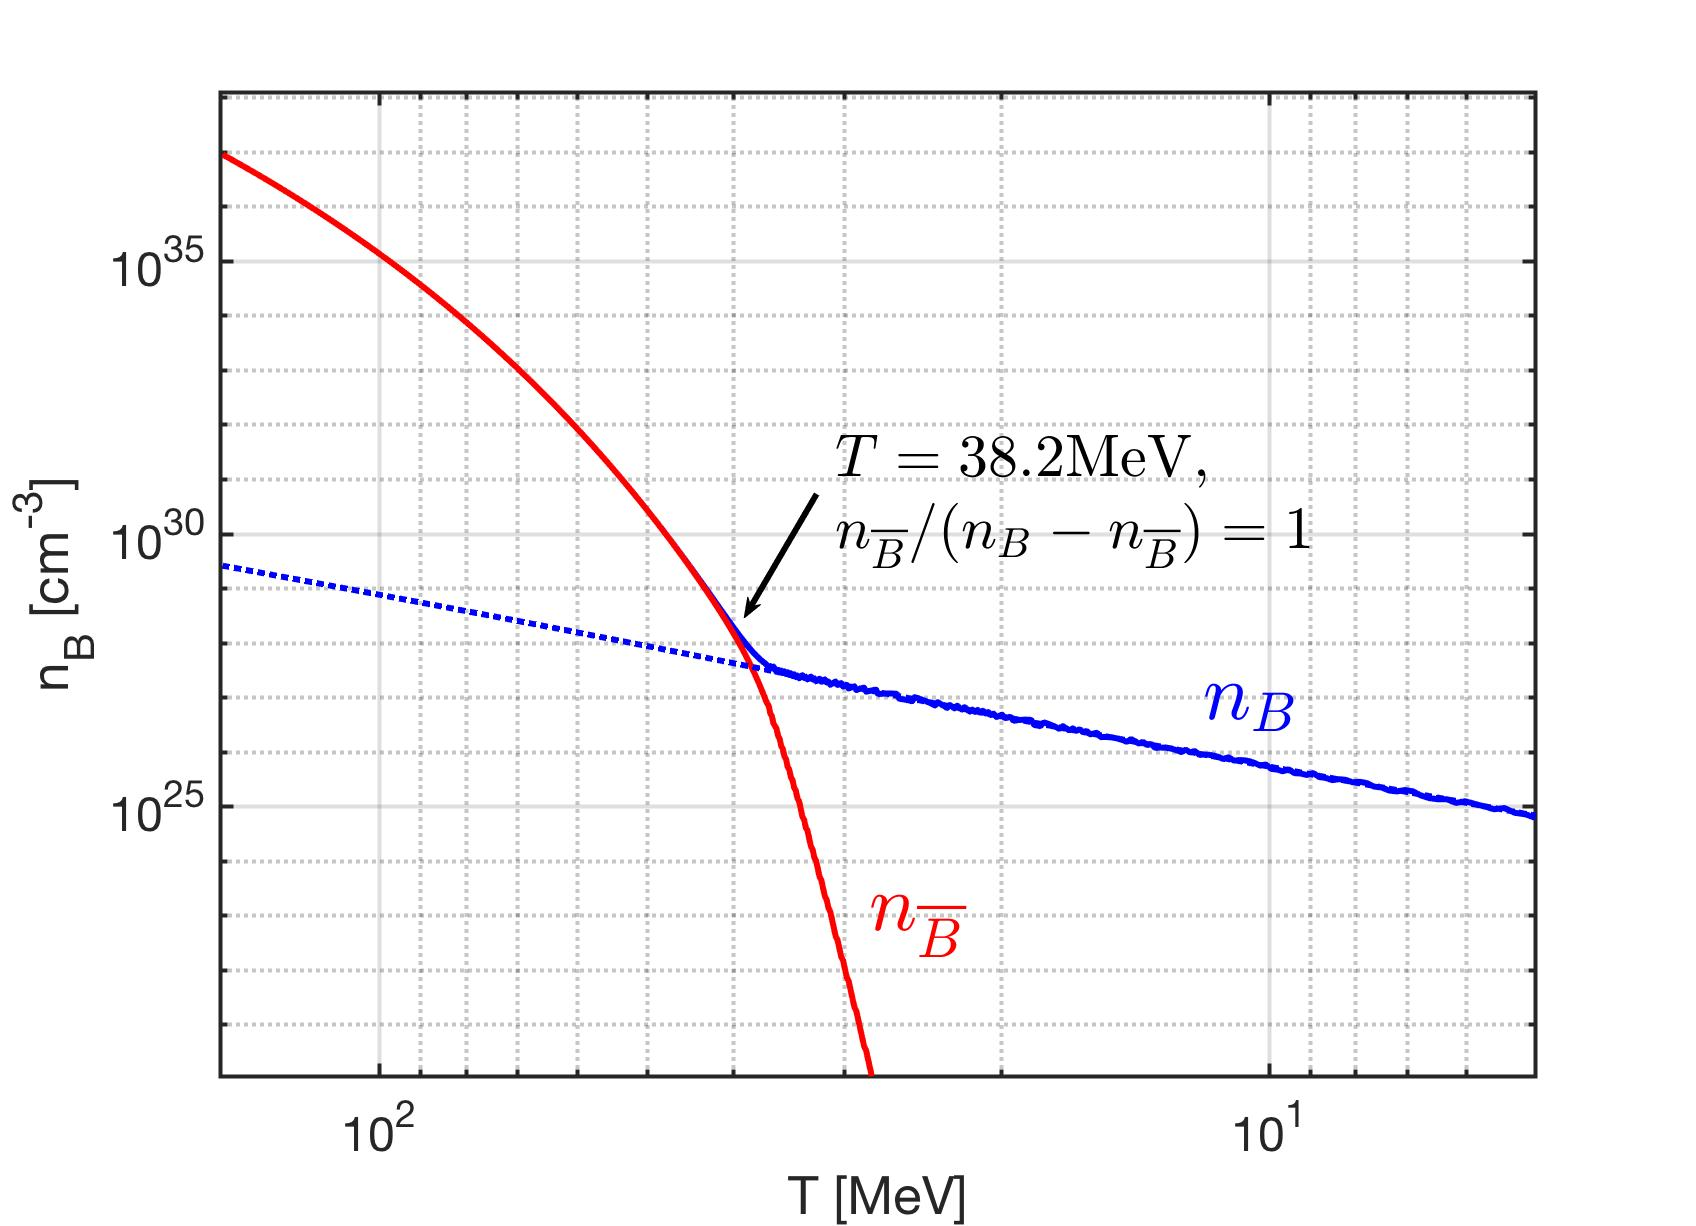
\includegraphics[width=0.9\linewidth]{./plots/Baryon_Antibaryon_cm.jpg}}
\caption{The antibaryon $n_{\overline  B}$ (red solid line) number density as a function of temperature in the range $150\MeV>T>5\MeV$. The blue solid line for baryons  $n_{B}$ merges into the antibaryon yield so that net baryon number $n_{B}-n_{\overline r B}$ (dashed blue line) continues the net  baryon yield seen as solid blue line. At temperature $T=38.2\MeV$  we have $n_{\overline B}/(n_B-n_{\overline B})=1$, antibaryons disappear from the Universe. \cccite{Rafelski:2023emw}. \radapt{Yang:2024ret}}
\label{Baryon:fig}\index{antibaryon!yield}
\end{figure}
%%%%%%%%%%%%%%%%%%%%%%%%%%%%%%%%%%%%%%%

In~\rf{Baryon:fig} we plot the number density of antibaryons (red line),  baryons (solid blue) and net baryon $n_B-n_{\overline B}$ (dashed blue) as a function of temperature. We determine the value of temperature $T=38.2\MeV$ to correspond to the condition $n_{\overline B}\ll(n_B-n_{\overline B})=1$, the effective antibaryon  disappearance temperature from the Universe inventory   $T=38.2\MeV$ is in agreement with the qualitative result presented in 1990 by Kolb and Turner~\cite{Kolb:1990vq}. Below this temperature, there antibaryons rapidly disappear, the net baryon density is the baryon asymmetry which dilutes keeping baryon to entropy ratio constant.

In~\rf{EquilibPartRatiosFig} we show examples of particle abundance ratios of interest\index{hadron!ratios}.   Pions $\pi(q\bar q)$ are the most abundant hadrons $n_\pi/n_B\gg1$, because of their low mass and the reaction $\gamma\gamma\rightarrow\pi^0$, which assures chemical yield equilibrium~\cite{Kuznetsova:2008jt} in the era of interest here. For $150\MeV>T>20.8\MeV$, we see the ratio $n_{{\overline K}(\bar q s)}/n_B\gg1$, which implies pair abundance of strangeness is more abundant than baryons, and is dominantly present in mesons, since $n_{\overline K}/n_Y\gg1$.  Considering $n_Y/n_B$ we see that hyperons $Y(sqq)$ remain a noticeable 1\% component in the baryon yield through the domain of antibaryon decoupling.

%%%%%%%%%%%%%%%%%%%%%%%%%%%%
\begin{figure} 
\centerline{
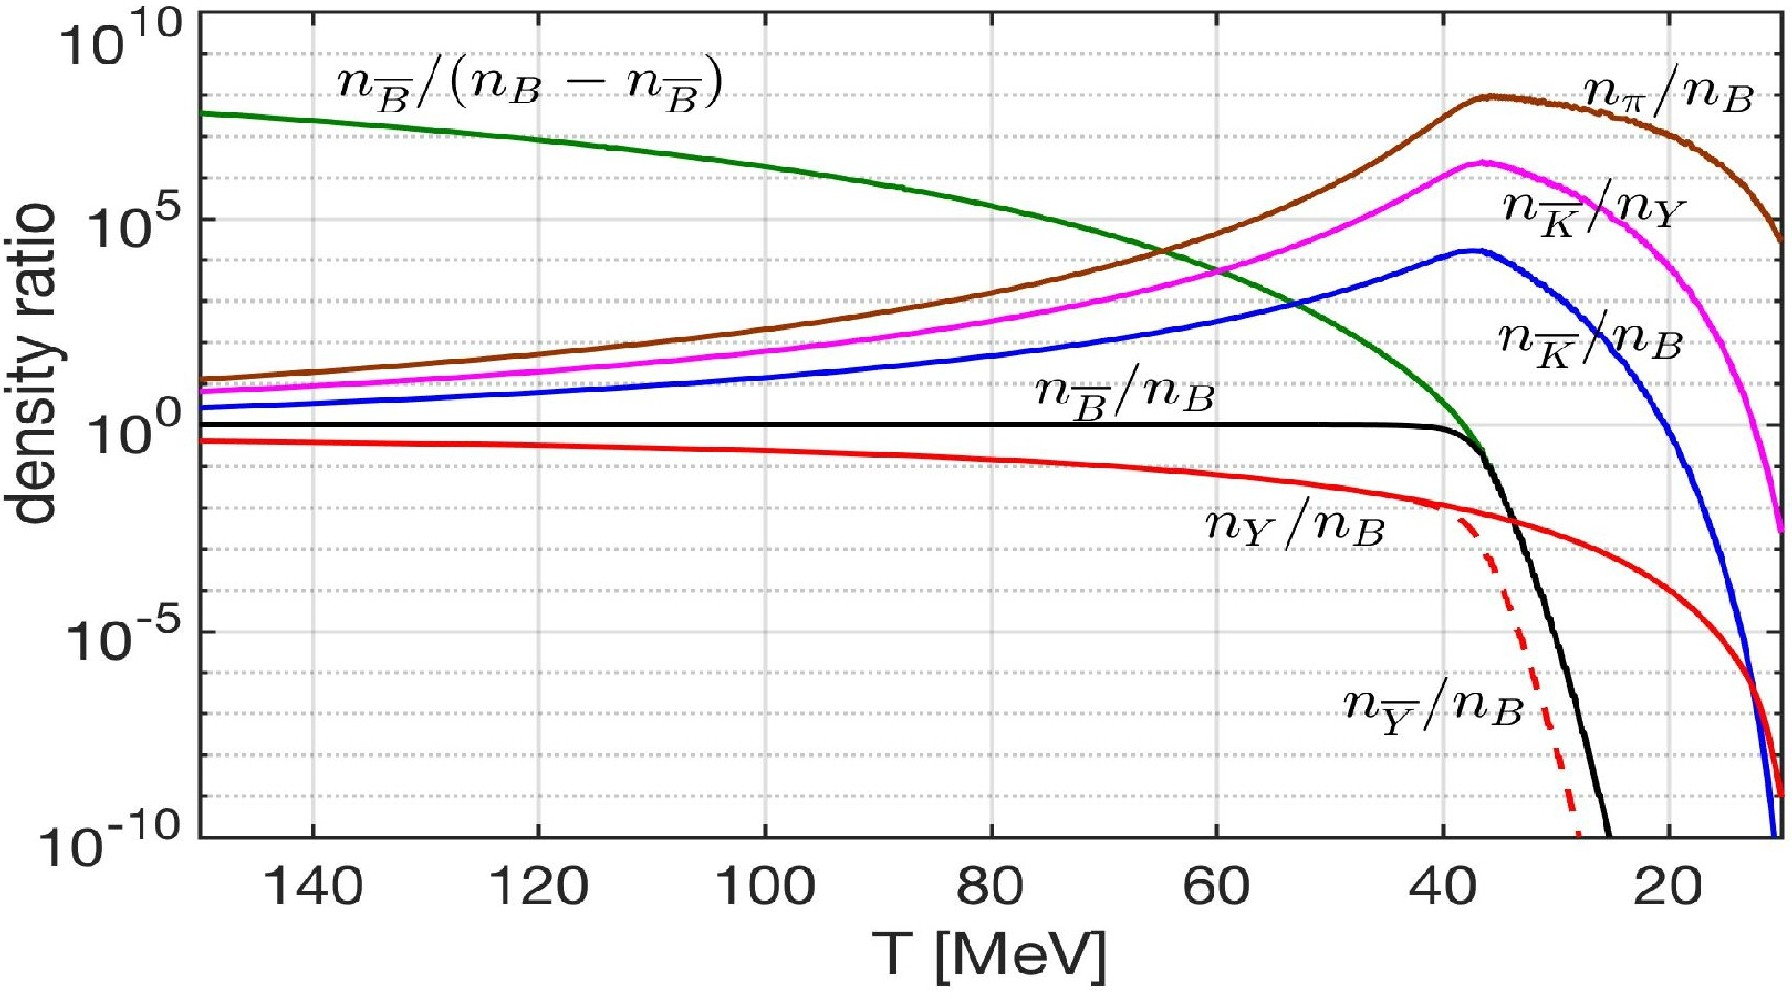
\includegraphics[width=0.9\linewidth]{./plots/Meson_Baryon_density_ratio_C.jpg}}
\caption{Ratios of hadronic particle number densities  with baryon $B$ yields as a function of temperature $150\MeV> T>10\MeV$: Pions $\pi$ (brown line), kaons $K( q\bar s)$ (blue), antibaryon $\overline B$ (black), hyperon $Y$ (red) and anti-hyperons $\overline Y$ (dashed red). Also shown $\overline K/Y$(purple). \cccite{Rafelski:2023emw}. \radapt{Yang:2021bko}}
\label{EquilibPartRatiosFig} 
\end{figure}
%%%%%%%%%%%%%%%%%%%%%%%%%%%
\index{strangeness!equilibrium among baryons and mesons} 

For $20.8\MeV>T$, the  baryon abundance becomes dominant over strange mesons $n_{\overline K}/n_B<1$, which implies that the strange meson is embedded in a large background of baryons, and the exchange reaction $\overline{K}+N\rightarrow \Lambda+\pi$ can re-equilibrate kaons and hyperons in the temperature range; therefore strangeness symmetry $s=\bar s$ can be maintained. For $12.9\MeV>T$ we have $n_Y/n_B>n_{\overline K}/n_B$, now the still existent tiny abundance of strangeness is found predominantly in hyperons.

%%%%%%%%%%%%%%%%%%%%%%%%%%%%%%%%%
\para{Strangeness dynamic population}\index{strangeness!dynamic population}
Given the equilibrium abundances of hadrons in the epoch of interest is $150\MeV\ge T\ge 10\MeV$ we turn now to study the freeze-out temperature for different particles and strangeness  by comparing the relevant reaction rates with each other and with the Hubble expansion rate.  We will need to explore a large number of reactions, going well beyond the relative simplicity of the case of QGP phase of matter. We find that strangeness is kept in equilibrium in the primordial Universe down until $T\approx 13\MeV$. This study addresses non-interacting particles, nuclear interactions can be many times greater compared to this temperature. Thus further exploration of this result seems necessary in the future.

Let us first consider an unstable strange particle $S$ decaying into two particles $1$ and $2$, which themselves have no strangeness content. In a dense and high-temperature plasma with particles $1$ and $2$ in thermal equilibrium, the inverse reaction populates the system with particle $S$. This is written schematically as
\begin{align}
 S\Longleftrightarrow1+2,\qquad \mathrm{Example}: K^0\Longleftrightarrow\pi+\pi\,.
\end{align}
As long as both decay and production reactions are possible, particle $S$ abundance remains in thermal equilibrium; as already discussed this balance between production and decay rates is the `detailed balance'.

Once the primordial Universe expansion rate $1/H$ overwhelms the strongly temperature dependent back-reaction and the back reaction freeze-out, then the decay $S\rightarrow 1+2$ occurs out of balance and particle $S$ disappears rather rapidly from the inventory. 

Second on our list are the two-on-two strangeness producing and burnup reactions. These have a significantly higher strangeness production reaction threshold, thus especially near to strangeness decoupling their influence is negligible. Such reactions are more important near the QGP hadronization temperature $T_H\simeq 150\MeV$. Typical  strangeness exchange reaction is $\mathrm{K}+N\leftrightarrow \Lambda+\pi$, (see Chapter 18 in~Ref.\,\cite{Letessier:2002ony}).

In~\rf{Strangeness_map2} we show some reactions relevant to strangeness evolution in the considered Universe evolution epoch $150\MeV\ge T\ge 10\MeV$ and their pertinent reaction strength. Specifically:
\begin{itemize}
\item
We study strange quark abundance in baryons and mesons, considering both open and hidden strangeness (hidden: $s\bar s$-content). Important source reactions are $l^-+l^+\rightarrow\phi$, $\rho+\pi\rightarrow\phi$, $\pi+\pi\rightarrow K_\mathrm{S}$, $\Lambda \leftrightarrow \pi+ N$, and $\mu^\pm+\nu\rightarrow K^\pm$. 
\item
Muons and pions are coupled through electromagnetic reactions $\mu^++\mu^-\leftrightarrow\gamma+\gamma$ and $\pi\leftrightarrow\gamma+\gamma$ to the photon background and retain their chemical equilibrium until the temperature $T =4$\, MeV and $T=5\MeV$, respectively~\cite{Rafelski:2021aey,Kuznetsova:2008jt}. The large $\phi\leftrightarrow K+K$ rate assures $\phi$ and $K$ are in relative chemical equilibrium.
\end{itemize}

%%%%%%%%%%%%%%%%%%%%%%%%%%%%%%%%%%%%%%%
\begin{figure} 
\centerline{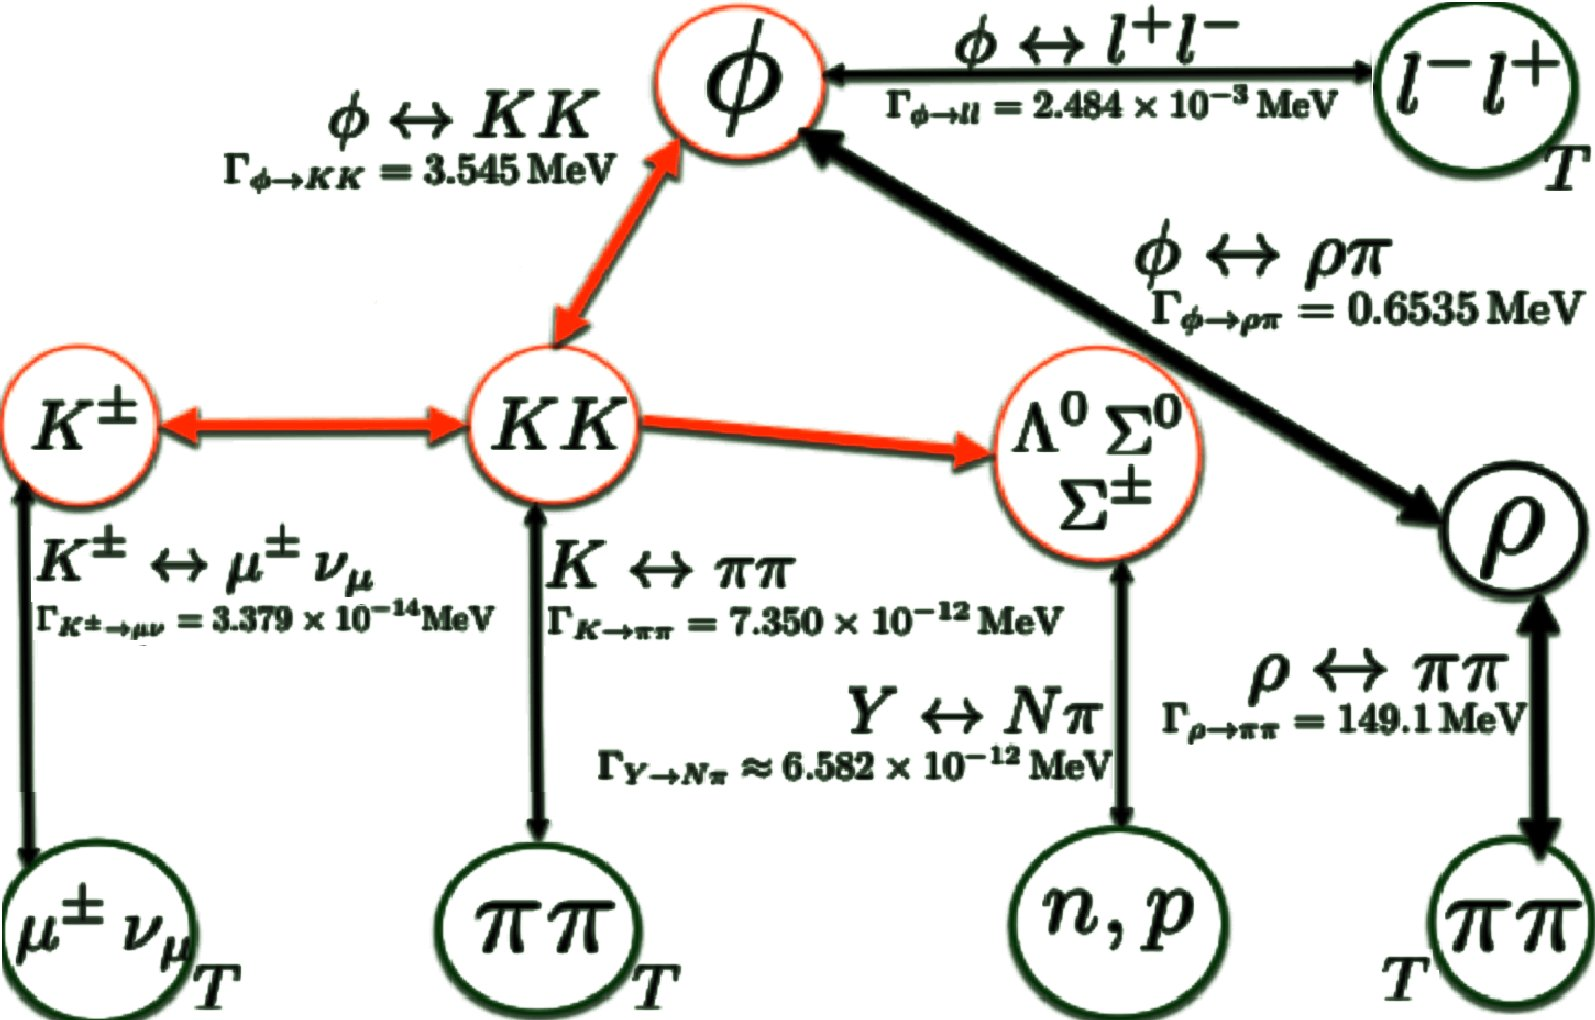
\includegraphics[width=0.9\linewidth]{./plots/Strangeness002_newJ.jpg}}
\caption{The strangeness abundance changing reactions in the primordial Universe. The red circles show strangeness carrying hadronic particles; red thick lines denote effectively instantaneous reactions. Black thick lines show relatively strong hadronic reactions. The reaction rates required to describe strangeness time evolution are presented in Ref.~\cite{Rafelski:2020ajx}. \cccite{Rafelski:2023emw}. \radapt{Yang:2024ret,Yang:2021bko}}
\label{Strangeness_map2} 
\end{figure}
%%%%%%%%%%%%%%%%%%%%%%%%%%%%%%%%%%%%

In order to determine where exactly strangeness disappears from the Universe inventory, we explore the magnitudes of different rates of production and decay processes in mesons and hyperons.
 
%%%%%%%%%%%%%%%%%%%%%%%%%%%%%%%%%%%%%
\para{Strangeness creation and annihilation rates in mesons}
From~\rf{Strangeness_map2} in the meson domain, the relevant interaction rates competing with Hubble time are the reactions\index{strangeness!mesons production rate}
\begin{align}
 &\pi+\pi\leftrightarrow K\,,\quad\mu^\pm+\nu\leftrightarrow K^\pm\,,\quad l^++l^-\leftrightarrow\phi\,,\\
 &\rho+\pi\leftrightarrow\phi\,,\quad \pi+\pi\leftrightarrow\rho\,.
\end{align}
The thermal reaction rate per time and volume for two body-to-one particle reactions $1+2\rightarrow 3$ has been presented before~\cite{Koch:1986ud,Kuznetsova:2008jt,Kuznetsova:2010pi}. 

In full kinetic and chemical equilibrium, the reaction rate per time per volume can be written as~\cite{Kuznetsova:2010pi} :\index{inverse decay rate}
\begin{align}
&R_{12\to 3}=\frac{g_3}{(2\pi)^2}\,\frac{m_3}{\tau^0_3}\,\int^\infty_0\frac{p^2_3dp_3}{E_3}\frac{e^{E_3/T}}{e^{E_3/T}\pm1}\Phi(p_3)\;,
\end{align}
where $\tau^0_3$ is the vacuum lifetime of particle $3$. The positive sign `$+$' is for the case when particle $3$ is a boson, and negative sign `$-$' for a fermion. The function $\Phi(p_3)$ for the nonrelativistic limit $m_3\gg p_3,T$ can be written as 
\begin{align}
\Phi(p_3\to0)=2\frac{1}{(e^{E_1/T}\pm1)(e^{E_2/T}\pm1)}.
\end{align}

Considering the Boltzmann limit, the thermal reaction rate per unit time and volume becomes
\begin{align}
\label{Thermal_Rate}
R_{12\rightarrow3}=\frac{g_3}{2\pi^2}\left(\frac{T^3}{\tau^0_3}\right)\left(\frac{m_3}{T}\right)^2\,K_1(m_3/T),
\end{align}
where $K_1$ is the modified Bessel functions of integer order `$1$'. 

In order to compare the reaction time with Hubble time $1/H$, it is convenient to define the relaxation time for the process $1+2\rightarrow 3$ as follows:
\begin{align}
\label{Reaction_Time}
\tau_{12\rightarrow 3}\equiv\frac{n^{eq}_{1}}{R_{12\rightarrow n}}\,,\quad
n^{eq}_1=\frac{g_1}{2\pi^2}\int_{m_1}^\infty\!\!\!\!dE\,\frac{E\,\sqrt{E^2-m_1^2}}{\exp{\left(E/T\right)}\pm1}\;, 
\end{align}
where $n^{eq}_1$\,is the thermal equilibrium number density of particle\,$1$ with the `heavy' mass $m_1>T$. Combining \req{Thermal_Rate} with \req{Reaction_Time} we obtain
\begin{align}\label{RelaxationTime}
&\frac{\tau_{12\rightarrow3}}{ \tau^0_3}= 
\frac{2\pi^2 n^{eq}_1/T^3}{g_3(m_3/T)^2\,K_1(m_3/T)}\,, \quad 
n^{eq}_1\simeq g_1\left(\frac{m_1 T}{2\pi}\right)^{3/2}e^{-m_1/T}\,,
\end{align}
where, conveniently, the relaxation time does not depend on the abundant and often relativistic heat bath component $2$, \eg\ $l^\pm,\pi,\nu,\gamma$. The density of heavy particles\,$1$\,and\,$3$ can in general be well approximated using the leading and usually nonrelativistic Boltzmann term as shown above.

In general, the reaction rates for inelastic collision process capable of changing particle number, for example $\pi\pi\to K^0$, is suppressed by the factor $\exp{(-m_{K^0}/T)}$. On the other hand, there is no suppression for the elastic momentum and energy exchanging particle collisions in plasma. In general for the case $m\gg T$, the dominant collision term in the relativistic Boltzmann equation is the elastic collision term, keeping all heavy particles in kinetic energy equilibrium with the plasma. This allows us to study the particle abundance in plasma presuming the energy-momentum statistical distribution  equilibrium shape exists.  This insight was discussed in detail in the preparatory phase of laboratory exploration of hot hadron and quark matter, see~\cite{Koch:1986ud}. 

In order to study the particle abundance in the Universe when $m\gg T$, instead of solving the exact Boltzmann equation, we can separate the fast energy-momentum equilibrating collisions from the slow particle number changing inelastic collisions. This approach makes it possible to explore the rates of inelastic collision and compare the relaxation times of particle production in all relevant reactions with the Universe expansion rate at a fixed temperature which governs the shape of particle distributions.

It is common to refer to particle freeze-out as the epoch where a given type of particle ceases to interact with other particles. In this situation the particle abundance decouples from the cosmic plasma, a chemical nonequilibrium and even complete abundance disappearance of this particle can accompany this; the condition for the given reaction $1+2\rightarrow 3$ to decouple is
\begin{align}
\tau_{12\rightarrow 3}(T_f)=1/H(T_f),
\end{align}
where $T_f$ is the freeze-out temperature.

In the epoch of interest, $150\MeV>T>10\MeV$, the Universe is dominated by radiation and effectively massless matter behaving like radiation. The Hubble parameter can be obtained from the Hubble equation and written as~\cite{Kolb:1990vq}
\begin{align}\label{H2g}
H^2=H^2_{rad}\left(1+\frac{\rho_{\pi,\,\mu,\,\rho}}{\rho_\mathrm{rad}}+\frac{\rho_\mathrm{strange}}{\rho_\mathrm{rad}}\right)=\frac{8\pi^3G_\mathrm{N}}{90}g^e_\ast T^4,\qquad H^2_\mathrm{rad}=\frac{8\pi G_\mathrm{N}\,\rho_\mathrm{rad}}{3},
\end{align}
where: $g^e_\ast$ is the total number of effective relativistic `energy' degrees of freedom; $G_\mathrm{N}$ is the Newtonian constant of gravitation; the `radiation' energy density includes $\rho_\mathrm{rad}=\rho_\gamma+\rho_\nu+\rho_{e^\pm}$ for photons, neutrinos, and massless electrons(positrons). The massive-particle correction is $\rho_{\pi,\,\mu,\,\rho}=\rho_\pi+\rho_\mu+\rho_\rho$; and at highest $T$ of interest, also of (minor) relevance, $\rho_\mathrm{strange}=\rho_{K^0}+\rho_{K^\pm}+\rho_{K^\ast}+\rho_{\eta}+\rho_{\eta^\prime}$.
Equating $1/H$ to the computed reaction rate we obtain the freeze-out temperature $T_f$. 

When considering the reaction rates and quoting $T_f$,   we must check allowing for a finite reaction time how sudden the freeze-out happens. We refer to this temperature uncertainty as  $\Delta T_f$, which by a simple scale consideration can be defined by
\begin{equation}\label{eq:DeltaT}
\Delta T_f\simeq \frac{1}{R(T_f)}\times \frac{dT}{dt}\,. 
\end{equation}
$R$\,[MeV] is the value of reaction rate at freeze-out. The greater is the rate $R_f$ the sharper is the freeze-out, thus smaller $\Delta T_f$.\index{freeze-out!uncertainty}

For the temperature range $50\MeV>T>5\MeV$, we have $10^{-1}<dT/dt<10^{-4}\MeV$/$\mu$s. We estimate the  width of freeze-out temperature interval $\Delta T_f$ using reaction rates for $dt$ as follows
\begin{align}
\frac{1}{\Delta T_f}\equiv \left[\frac{1}{(\Gamma_{12\to3}/H)}\frac{d(\Gamma_{12\to3}/H)}{dT}\right]_{T_f},\quad \Gamma_{12\to3}\equiv\frac{1}{\tau_{12\to3}}.
\end{align}
Using \req{H2g} and \req{RelaxationTime} and considering the temperature range $50\MeV>T>5\MeV$ with $g^e_\ast\approx\mathrm{constant}$ we obtain using the Boltzmann approximation to describe the massive particles\,$1$\,and\,$3$
\begin{align}\label{DeltaFreezeout}
 \frac{\Delta T_f}{ T_f} \approx\frac{T_f }{ m_3 - m_1 -2T_f}\,,\quad m_3 - m_1>> T_f\,.
\end{align}
The width of freeze-out domain is shown in the right column in Table~\ref{FreezeoutTemperature_table}. We see a range of $2$-$10\%$. Therefore it is nearly justified to consider as a decoupling condition in time the value of temperature at which the pertinent rate crosses the Hubble expansion rate, see~\rf{reaction_time_tot}.\index{freeze-out!duration}
 
%%%%%%%%%%%%%%%%%%%%%%%%%%%
\begin{table} 
\centering
\begin{tabular}{c| c| c}
\hline\hline
Reactions &Freeze-out $T_f$\,[MeV] & {Uncertainty $\Delta T_f$\,[MeV]} \\
\hline
$\mu^\pm\nu\rightarrow K^\pm$ & $T_f=33.8\MeV$ & {$3.5$ \,MeV}\\ 
\hline
$e^+e^-\rightarrow \phi$ & $T_f=24.9\MeV$ &{$0.6\MeV$}\\
$\mu^+\mu^-\rightarrow\phi$ & $T_f=23.5\MeV$ &{$0.6\MeV$}\\
\hline
 $\pi\pi\rightarrow K$ & $T_f=19.8\MeV$&{$1.2\MeV$}\\
\hline
$\pi\pi\rightarrow\rho$ & $T_f=12.3\MeV$&{$0.2\MeV$}\\
\hline\hline
\end{tabular}
\caption{Strangeness producing reactions in primordial Universe, their freeze-out temperature $T_f$; and temperature uncertainty $\Delta T_f$}
\label{FreezeoutTemperature_table} 
\end{table}
%%%%%%%%%%%%%%%%%%%%%%%%%%%%%%%%%%%%%%

%%%%%%%%%%%%%%%%%%%%%%%%%%%%%%%%%%%%%%%%%
\begin{figure}
%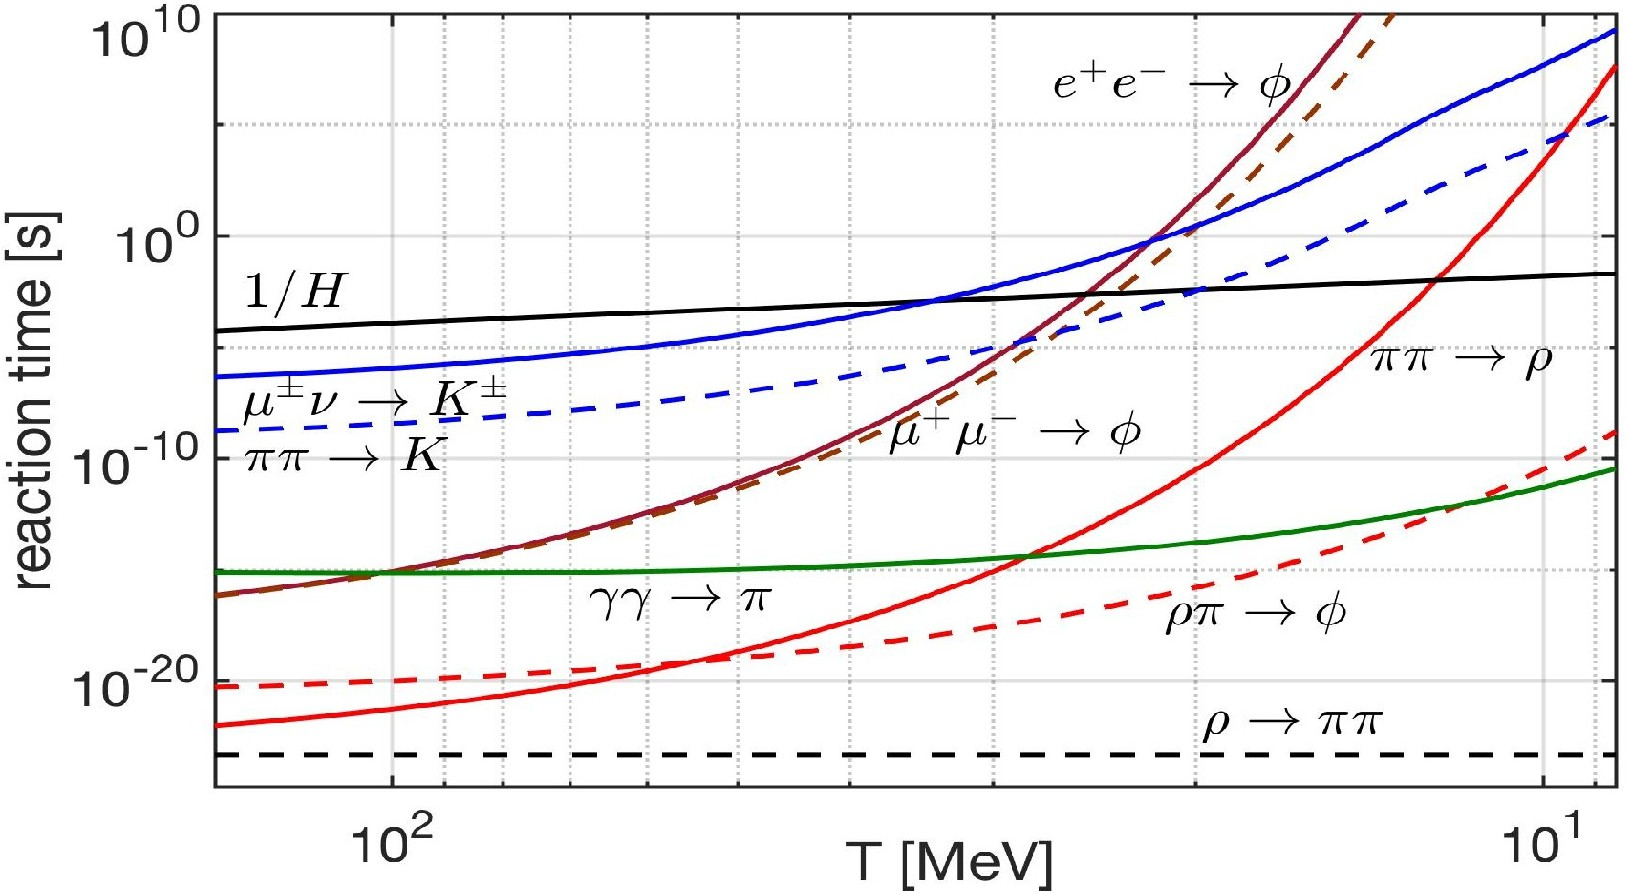
\includegraphics[width=0.95\linewidth]{./plots/Strangeness_Hubble_C.jpg}
\centerline{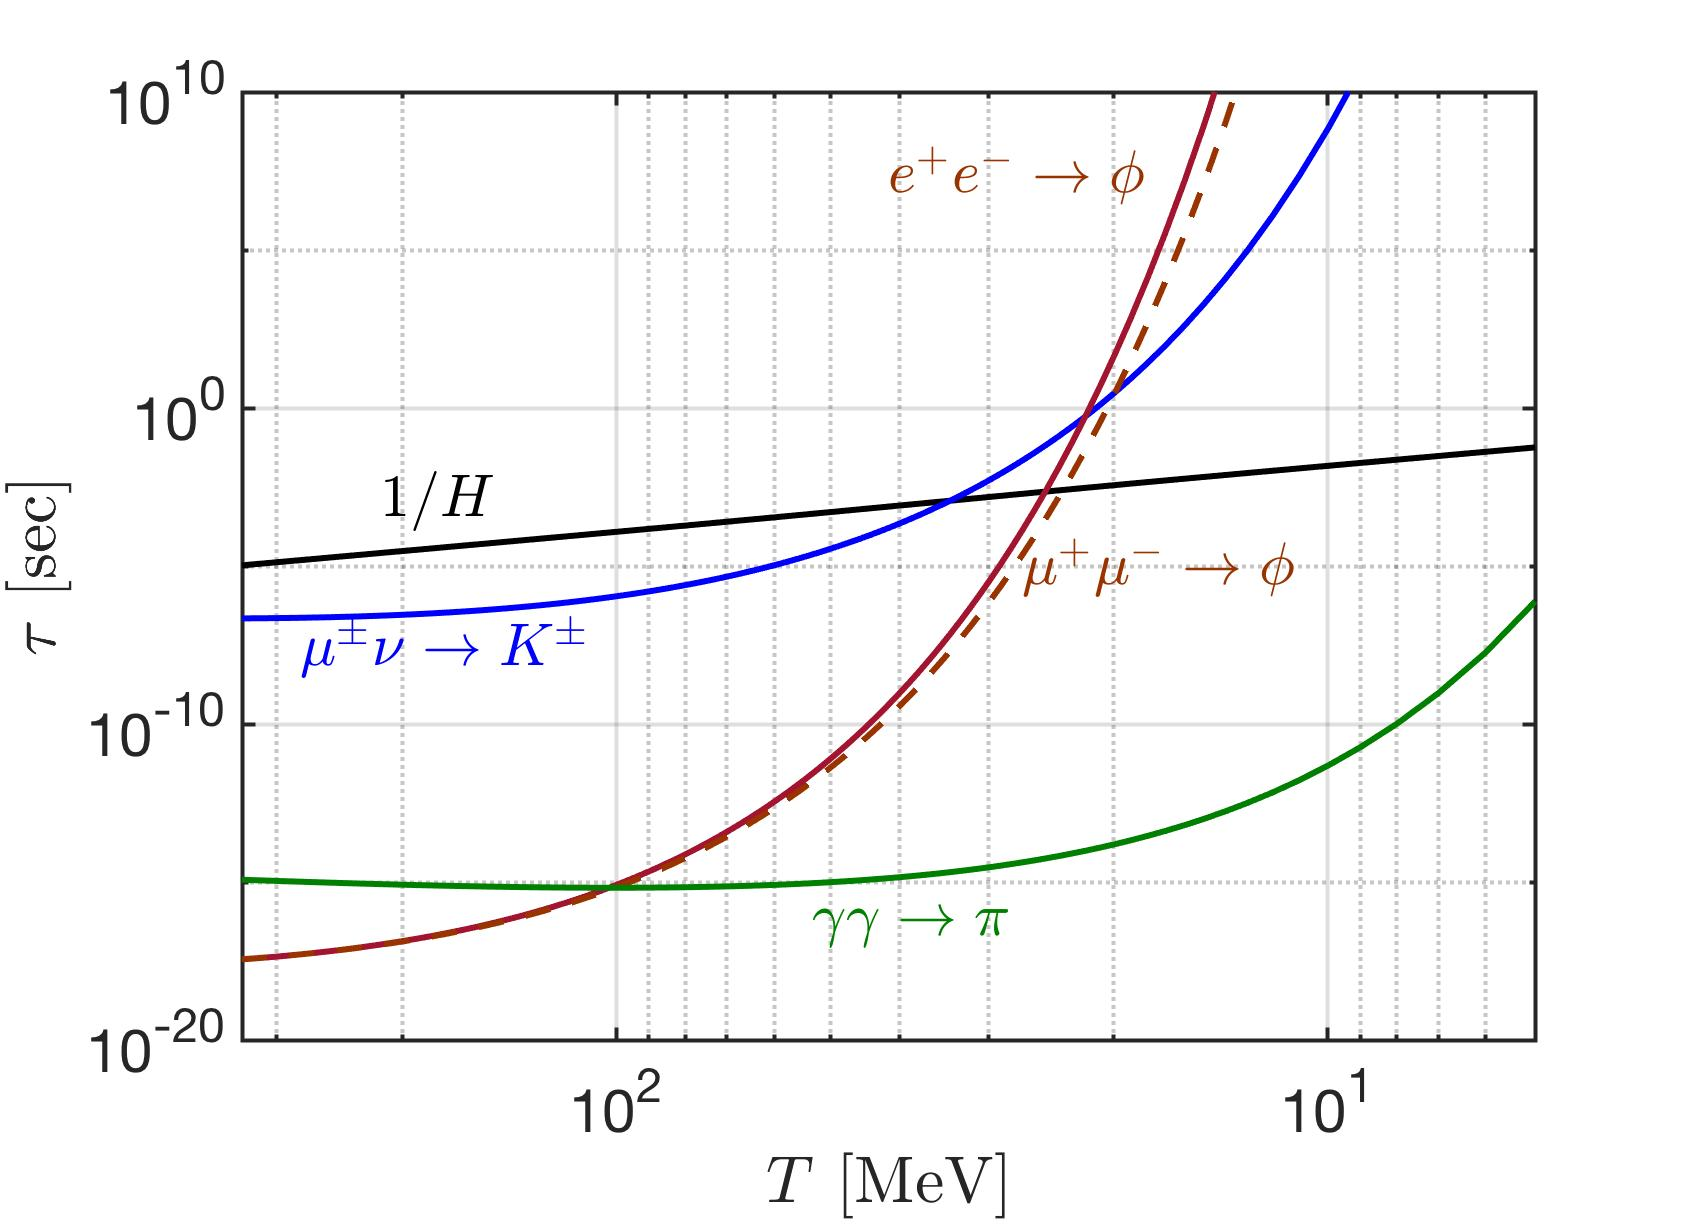
\includegraphics[width=0.9\linewidth]{./plots/Strangeness_Hubble002.jpg}}
\centerline{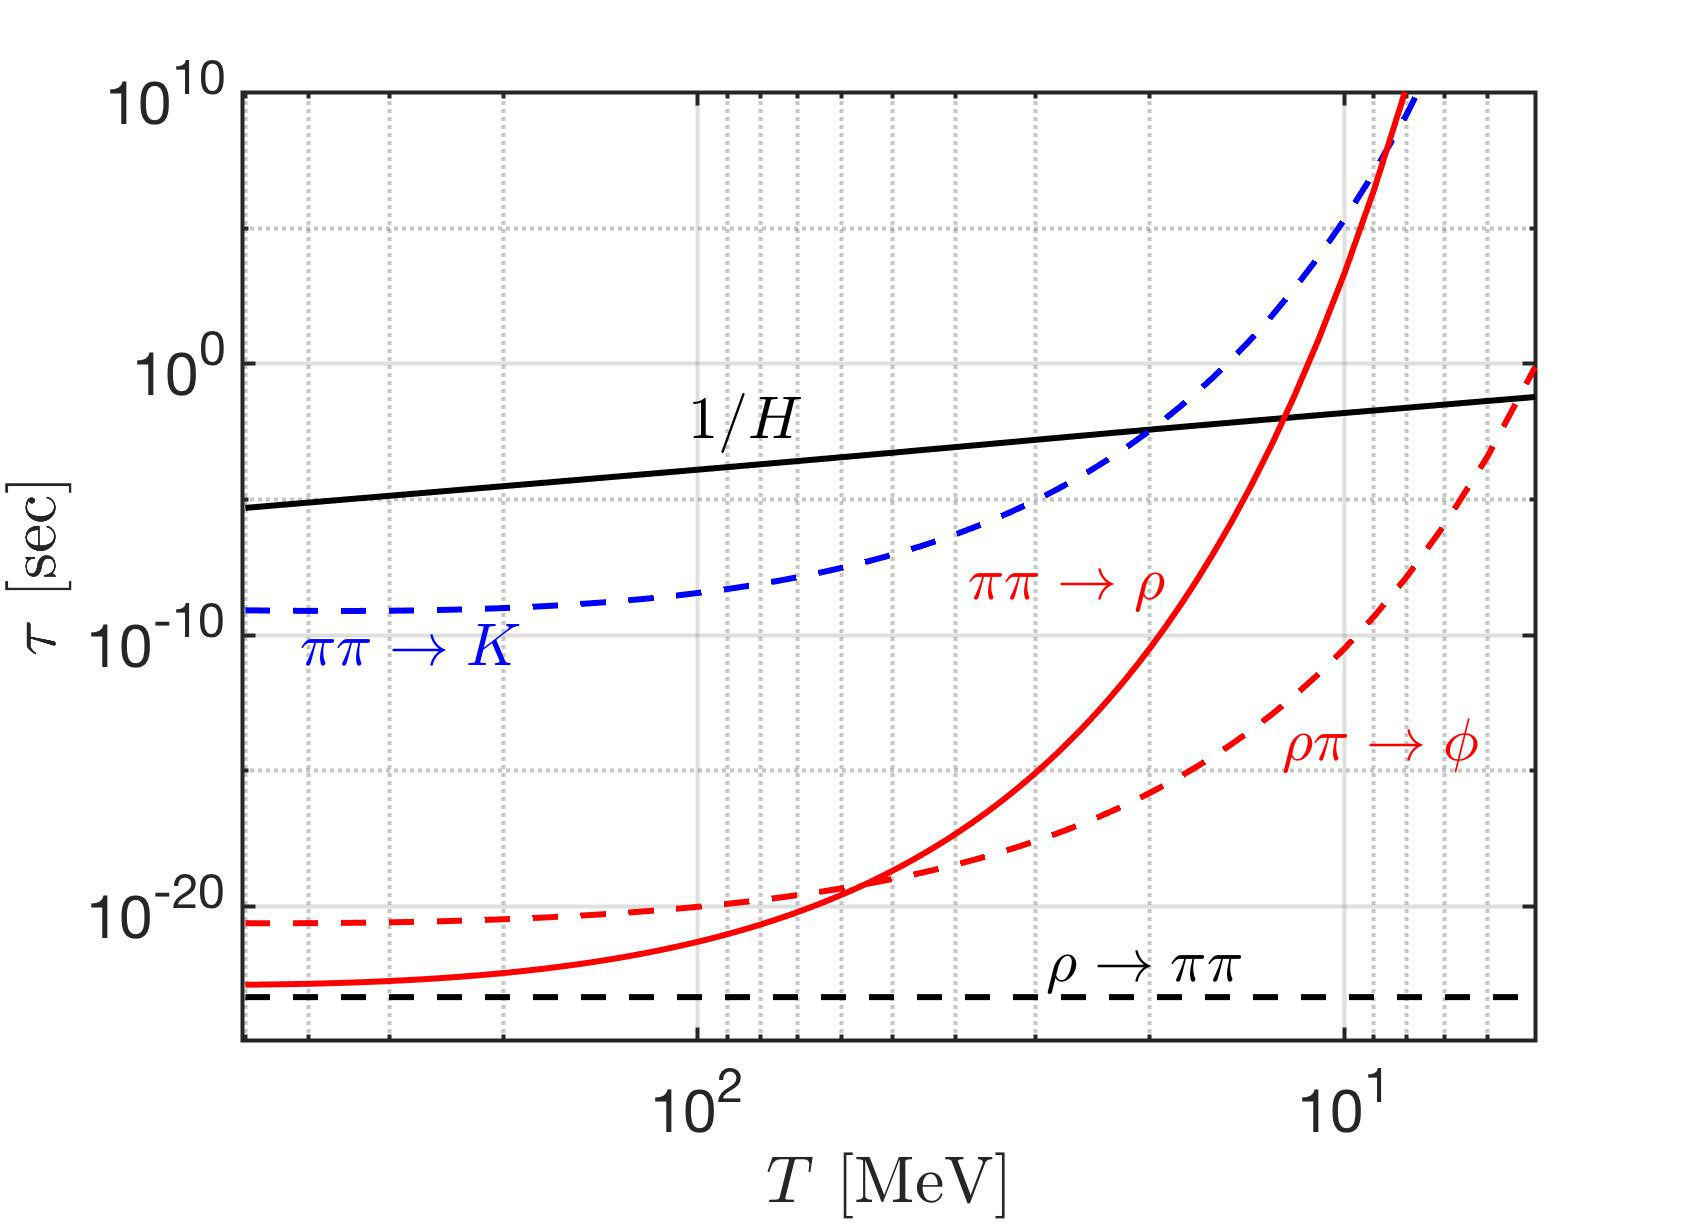
\includegraphics[width=0.9\linewidth]{./plots/Strangeness_Hubble003.jpg}}
\caption{Hadronic relaxation reaction times, see \req{Reaction_Time}, as a function of temperature $T$, are compared to Hubble time $1/H$ (black solid line). At bottom the horizontal black-dashed line is the natural (vacuum) lifespan of $\rho$. \cccite{Rafelski:2023emw}. \radapt{Yang:2024ret,Yang:2021bko}}
\label{reaction_time_tot} 
\end{figure}
%%%%%%%%%%%%%%%%%%%%%%%%

In~\rf{reaction_time_tot} we plot the hadronic reaction relaxation times $\tau_{i}$ in the meson sector as a function of temperature compared to Hubble time $1/H$. We note that the weak interaction reaction $\mu^\pm+\nu_{\mu}\rightarrow K^\pm$ becomes slower compared to the Universe expansion near temperature $T_f^{K^\pm}=33.8\MeV$, signaling the onset of abundance nonequilibrium for $K^\pm$. For $T<T_f^{K^\pm}$, the reactions $\mu^\pm+\nu_{\mu}\rightarrow K^\pm$ decouples from the cosmic plasma; the corresponding detailed balance can be broken and the decay reactions $K^\pm\rightarrow\mu^\pm+\nu_{\mu}$ are acting like a (small) ``hole'' in the strangeness abundance ``pot''. If other strangeness production reactions did not exist, strangeness would disappear as the Universe cools below $T_f^{K^\pm}$. However, there are other reactions: $l^++l^-\leftrightarrow\phi$, $\pi+\pi\leftrightarrow K$, and $\rho+\pi\leftrightarrow\phi$ can still produce the strangeness in cosmic plasma and the rate is very large compared to the weak interaction decay.

In Table~\ref{FreezeoutTemperature_table} we also show the characteristic strangeness reactions and their freeze-out temperatures in the primordial Universe. The intersection of strangeness reaction times with $1/H$ occurs for $l^-+l^+\rightarrow\phi$ at $T_f^\phi=25\sim23\MeV$, and for $\pi+\pi\rightarrow K$ at $T_f^K=19.8\MeV$, for $\pi+\pi\rightarrow\rho$ at $T_f^\rho=12.3\MeV$. The reactions $\gamma+\gamma\rightarrow\pi$ and $\rho+\pi\leftrightarrow\phi$ are faster compared to $1/H$. However, the $\rho\to\pi+\pi$ lifetime (black dashed line in~\rf{reaction_time_tot}) is smaller than the reaction $\rho+\pi\leftrightarrow\phi$; in this case, most of $\rho$-meson decays faster, thus are absent and cannot contribute to the strangeness creation in the meson sector. Below the temperature $T<20\MeV$, all the detail balances in the strange meson reactions are broken and the strangeness in the meson sector should disappear rapidly, were it not for the small number of baryons present in the Universe.

%%%%%%%%%%%%%%%%%%%%%%%%%%%%%%%%%%%%%%%%%%%%
\para{Strangeness production and exchange rates involving hyperons}\index{strangeness!hyperons}
In order to understand strangeness in hyperons in the baryonic domain, we now consider the strangeness production reaction $\pi +N\rightarrow K+\Lambda$, the strangeness exchange reaction $\overline{K}+N\rightarrow \Lambda+\pi$; and the strangeness decay $\Lambda\rightarrow N+\pi$. The competition between different strangeness reactions allows strange hyperons and antihyperons to influence the dynamic nonequilibrium condition, including development of $\langle s-\bar s\rangle \ne 0$.

To evaluate the reaction rate in two-body reaction $1+2\rightarrow3+4$ in the Boltzmann approximation we can use the reaction cross section $\sigma(s)$ and the relation~\cite{Letessier:2002ony}:\index{hyperon!production rate}
\begin{align}
R_{12\rightarrow34}=\frac{g_1g_2}{32\pi^4}\frac{T}{1+I_{12}}\!\!\int^\infty_{s_{th}}\!\!\!\!ds\,\sigma(s)\frac{\lambda_2(s)}{\sqrt{s}}\!K_1\!\!\left({\sqrt{s}}/{T}\right),
\end{align}
where $K_1$ is the Bessel function of order $1$ and the function $\lambda_2(s)$ is defined as
\begin{align}
\lambda_2(s)=\left[s-(m_1+m_2)^2\right]\left[s-(m_1-m_2)^2\right],
\end{align}
with $m_1$ and $m_2$, $g_1$ and $g_2$ as the masses and degeneracy of the initial interacting particle. The factor $1/(1+I_{12})$ is introduced to avoid double counting of indistinguishable pairs of particles; we have $I_{12}=1$ for identical particles and $I_{12}=0$ for others. 

The thermal averaged cross sections for the strangeness production and exchange processes are about $\sigma_{\pi N\rightarrow K\Lambda}\sim0.1\,\mathrm{mb}$ and $\sigma_{\overline{K}N\rightarrow \Lambda\pi}=1\sim3\,\mathrm{mb}$ in the energy range in which we are interested~\cite{Koch:1986ud}. The cross section can be parameterized as follows:\\
1) For the cross section $\sigma_{\overline{K}N\rightarrow \Lambda\pi}$ we use~\cite{Koch:1986ud}
 \begin{align}
 \sigma_{\overline{K}N\rightarrow \Lambda\pi}=\frac{1}{2}\left(\sigma_{K^-p\rightarrow \Lambda\pi^0}+\sigma_{K^-n\rightarrow \Lambda\pi^-}\right)\,.
\end{align}
Here the experimental cross sections can be parameterized as 
\begin{align}
&\sigma_{K^-p\rightarrow \Lambda\pi^0}\!\!=\!\!\left(\begin{array}{l}\!\!1479.53\mathrm{mb}\!\cdot\!\exp{\left(\frac{-3.377\sqrt{s}}{\mathrm{GeV}}\right)},\; \mathrm{for}\,\sqrt{s_m}\!\!<\!\!\sqrt{s}\!<\!3.2\mathrm{GeV} \\ \\0.3\mathrm{mb}\!\cdot\!\exp{\left(\frac{-0.72\sqrt{s}}{\mathrm{GeV}}\right)},\; \mathrm{for}\sqrt{s}>3.2\mathrm{GeV}\end{array}\right.\\
&\sigma_{K^-n\rightarrow \Lambda\pi^-}\!\!=\!\!1132.27\mathrm{mb}\!\cdot\!\exp{\left(\frac{-3.063\sqrt{s}}{\mathrm{GeV}}\right)},\; \mathrm{for}\sqrt{s}>1.699\mathrm{GeV},
\end{align}
where $\sqrt{s_m}=1.473\GeV$.\\
2) For the cross section $\sigma_{\pi N\rightarrow K\Lambda}$ we use~\cite{Cugnon:1984pm}
\begin{align}
&\sigma_{\pi N\rightarrow K\Lambda}=\frac{1}{4}\times\sigma_{\pi p\rightarrow K^0\Lambda}\,.
\end{align}
The experimental $\sigma_{\pi p\rightarrow K^0\Lambda}$ can be approximated as follows
\begin{align}
\sigma_{\pi p\rightarrow K^0\Lambda}=\left(\begin{array}{l}\frac{0.9\mathrm{mb}\cdot\left(\sqrt{s}-\sqrt{s_0}\right)}{0.091\mathrm{GeV}},\; \mathrm{for} \sqrt{s_0}<\sqrt{s}<1.7\mathrm{GeV} \\ \\ \frac{90\mathrm{MeV\cdot mb}}{\sqrt{s}-1.6\mathrm{GeV}},\; \mathrm{for}\sqrt{s}>1.7\mathrm{GeV},\end{array}\right.
 \end{align}
 with $ \sqrt{s_0}=m_\Lambda+m_K$. 

Given the cross sections, we obtain the thermal reaction rate per volume for strangeness exchange reaction seen in~\rf{Lambda_Rate_volume.fig}. We see that near to $T=20\MeV$, the dominant reactions for the hyperon $\Lambda$ production is $\overline{K}+N\leftrightarrow\Lambda+\pi$. At the same time, the $\pi+\pi\to K$ reaction becomes slower than Hubble time and kaon $K$ decay rapidly in the primordial Universe. However, the anti-kaons $\overline K$ produce the hyperon $\Lambda$ because of the strangeness exchange reaction $\overline{K}+N\rightarrow\Lambda+\pi$ in the baryon-dominated Universe. We have strangeness in $\Lambda$ and it disappears from the Universe via the decay $\Lambda\rightarrow N+\pi$. Both strangeness and anti-strangeness disappear because of the $K\rightarrow\pi+\pi$ and $\Lambda\rightarrow N+\pi$, while the strangeness abundance $s = \bar{s}$ in the primordial Universe remains.

%%%%%%%%%%%%%%%%%%%%%%%%%%%%%%%%
\begin{figure} 
\centerline{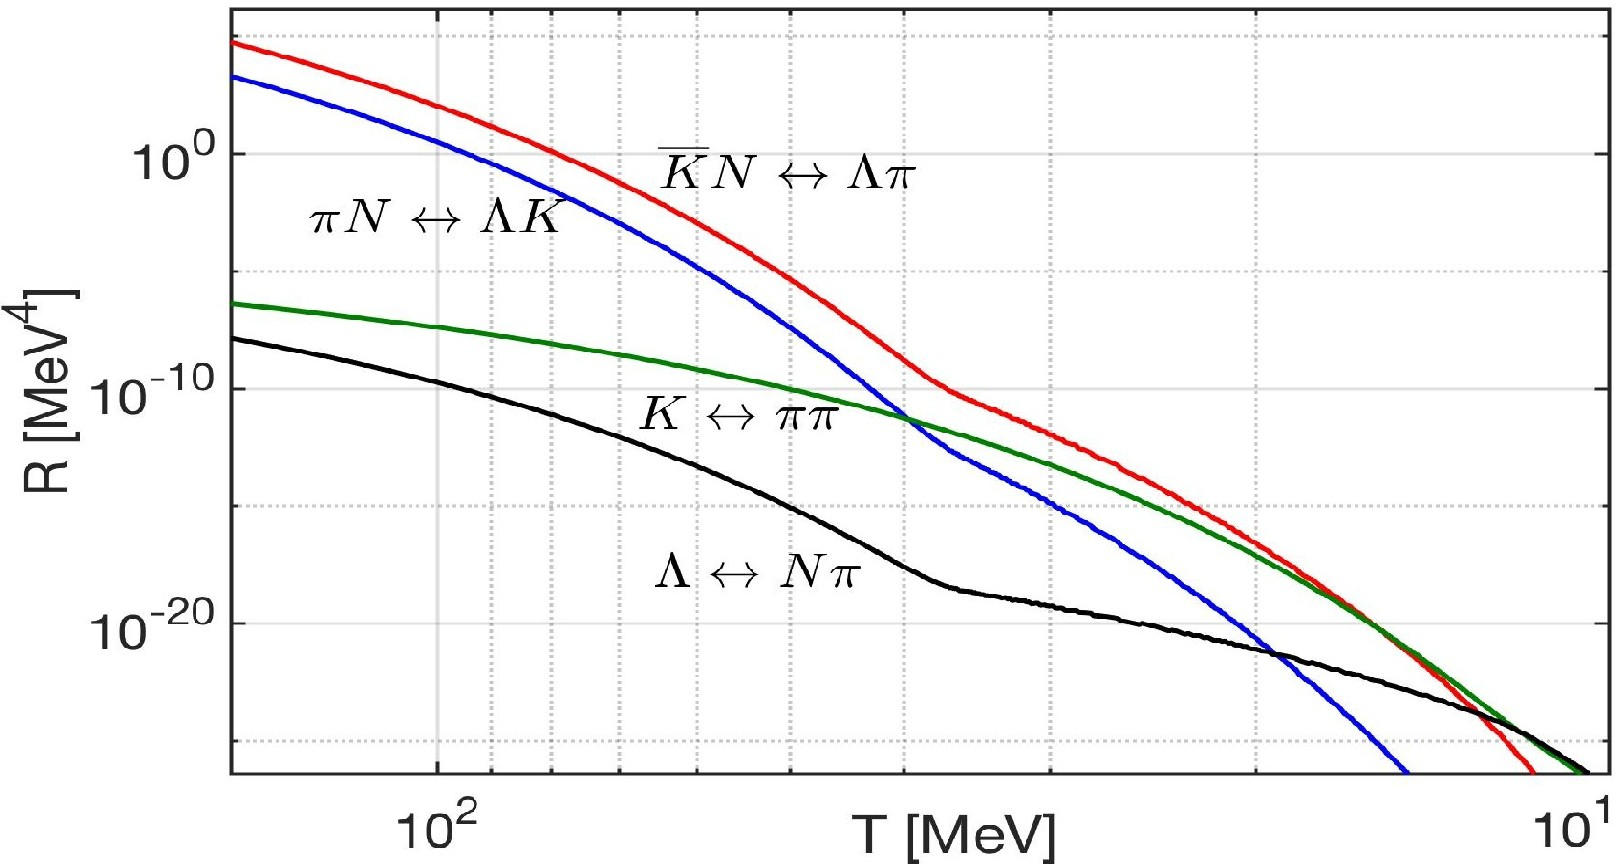
\includegraphics[width=0.9\linewidth]{./plots/NewHyperonRate_C.jpg}}
\caption{Thermal reaction rate $R$ per volume and time for important hadronic strangeness production and exchange processes as a function of temperature $150\MeV> T>10\MeV$ in the primordial Universe. \cccite{Rafelski:2023emw}. \radapt{Yang:2024ret,Yang:2021bko}}
\label{Lambda_Rate_volume.fig} 
\end{figure}
%%%%%%%%%%%%%%%%%%%%%%%%%%%%%%%%%%%%

Near to $T=12.9\MeV$ the reaction $\Lambda+\pi\rightarrow\overline{K}+N$ becomes slower than the strangeness decay $\Lambda\leftrightarrow N+\pi$ and shows that at the low temperature the $\Lambda$ particles are still in equilibrium via the reaction $\Lambda\leftrightarrow N+\pi$ and little strangeness remains in the $\Lambda$. Then strangeness abundance becomes asymmetric $s\gg \bar{s}$, which implies that the assumption for strangeness conservation can only be valid until the temperature $T\sim13\MeV$. Below this temperature a new regime opens up in which the tiny residual strangeness abundance is governed by weak decays with no re-equilibration with mesons. Also, in view of baron asymmetry, $\langle s-\bar s\rangle \ne 0$.

\section{Neutrino Plasma}\label{Neutrino}
\subsection{Neutrino properties and reactions}\label{ssec:nuproperties}
Neutrinos are fundamental particles which play an important role in the evolution of the Universe. In the early Universe the neutrinos are kept in equilibrium with cosmic plasma via the weak interaction. The neutrino-matter interactions plays a crucial role in  understanding of neutrinos evolution in the early Universe (such as neutrino freeze-out) and the later Universe (the property of today's neutrino background). In this chapter, we will examine the neutrino coherent and incoherent scattering with matter and their application in cosmology. The investigation of the relation between the effective number of neutrinos\index{neutrino!effective number} $N^{\mathrm{eff}}_\nu$ and lepton asymmetry\index{lepton!asymmetry} $L$ after neutrino freeze-out\index{neutrino!freeze-out} and its impact on Universe expansion is also discussed in this chapter. 

%%%%%%%%%%%%%%%%%%%%%%%%%%%%%%
\para{Matrix elements for neutrino coherent \& incoherent scattering}
 According to the standard model, neutrinos interact with other particles via the Charged-Current(CC) and Neutral-Current(NC) interactions. Their Lagrangian can be written as~\cite{Giunti:2007ry}
\begin{align}
&\mathcal{L}^{CC}=\frac{g}{2\sqrt{2}}\left(j^\mu_W\,W_\mu+{j^\mu_W}^\dagger\,W^\dagger_\mu\right),\qquad\mathcal{L}^{NC}=-\frac{g}{2\cos{\theta_w}}\,j^\mu_Z\,Z_\mu,
\end{align}
where $g=e\sin\theta_w$, $W^\mu$ and $Z^\mu$ are W and Z boson gauge fields, and $j^\mu_W$ and $j^\mu_Z$ are the charged-current and neutral-current separately. In the limit of energies lower than the $W(m_w=80\,\mathrm{GeV})$ and $Z(m_z=91\,\mathrm{GeV})$ gauge bosons, the effective Lagrangians are given by
\begin{align}\label{L_low}
\mathcal{L}^{CC}_{eff}=-\frac{G_F}{\sqrt{2}}\,j^\dagger_{W\,\mu}\,j^\mu_W,\qquad
\mathcal{L}^{NC}_{eff}=-\frac{G_F}{\sqrt{2}}\,j^\dagger_{Z\,\mu}\,j^\mu_Z,\qquad \frac{G_F}{\sqrt{2}}=\frac{g^2}{8m^2_W},
\end{align}
where $G_F=1.1664\times10^{-5}\,\mathrm{GeV}^{-2}$ is the Fermi constant, which is one of the important parameters that determine the strength of the weak interaction rate. When neutrinos interact with matter, based on the neutrino's wavelength, they can undergo two types of scattering processes: coherent scattering and incoherent scattering with the particles in the medium. 

With coherent scattering, neutrinos interact with the entire  composite system rather than individual particles within the system. The coherent scattering is particularly relevant for low-energy neutrinos when the wavelength of neutrino is much larger than the size of system. In $1978$, Lincoln Wolfenstein pointed out that the coherent forward scattering of neutrinos off matter could be very important in studying the behavior of neutrino flavor oscillation\index{neutrino!flavor oscillation} in a dense medium~\cite{Wolfenstein:1977ue}. The fact that neutrinos propagating in matter may interact with the background particles can be described by the picture of free neutrinos traveling in an effective potential.

For incoherent scattering, neutrinos interact with particles in the medium individually. Incoherent scattering is typically more prominent for high-energy neutrinos, where the wavelength of neutrino is smaller compared to the spacing between particles. Study of incoherent scattering of high-energy neutrinos is important for understanding the physics in various astrophysical systems (e.g. supernova, stellar formation) and the evolution of the early Universe.

In this section, we discuss the coherent scattering between long wavelength neutrinos and atoms, and study the effective potential for neutrino coherent interaction. Then we present the matrix elements that describe the incoherent interaction between high energy neutrinos and other fundamental particles in the early Universe. Understanding these matrix elements is crucial for comprehending the process of neutrino freeze-out in the early Universe.

%%%%%%%%%%%%%%%%%%%%%%%%%%%%%%%%
\para{Long wavelength limit of neutrino-atom coherent scattering}
%\label{LongWavelength}
According to the standard cosmological model, the Universe today is filled with the cosmic neutrinos with temperature $T_{\nu}^0=1.9 \,\mathrm{K}=1.7\times10^{-4}\,\mathrm{eV}$. The average momentum of present-day relic neutrinos is given by $\langle p_\nu^0\rangle\approx3.15\,T_\nu^0$ and the typical wavelength $\lambda_{\nu}^{0}={2\pi}/{\langle p_{\nu}^{0}\rangle}\approx2.3\times10^5\,$\AA, which is much larger than the radius at the atomic scale, such as the Bohr radius $R_{\mathrm{atom}}=0.529\,$\AA. In this case we have the long wavelength condition $\lambda_\nu\gg\,R_{\mathrm{atom}}$ for cosmic neutrino background today.  

Under the condition $\lambda_\nu\gg\,R_{\mathrm{atom}}$, when the neutrino is scattering off an atom, the interaction can be coherent scattering~\cite{PhysRevD.38.32,Lewis:1979mu,Papavassiliou:2005cs}. According to the principles of quantum mechanics, with neutrino scattering it is impossible to identify which scatters the neutrino interacts with and thus it is necessary to sum over all possible contributions. In such circumstances, it is appropriate to view the scattering reaction as taking place on the atom as a whole, i.e.,\index{neutrino!coherent scattering}
\begin{align}
\nu+\mathrm{Atom}\longrightarrow\nu+\mathrm{Atom}.
\end{align}

Considering a neutrino elastic scattering off an atom which is composed of $Z$ protons, $N$ neutrons and $Z$ electrons. For the elastic neutrino atom scattering, the low-energy neutrinos scatter off both atomic electrons and nucleus. For nucleus parts, we consider that the neutrinos interact via the $Z^0$ boson with a nucleus as
\begin{align}
\nu+A^{Z}_N\longrightarrow\nu+A^{Z}_N.
\end{align}
In this process a neutrino of any flavor scatters off a nucleus with the same strength. Therefore, the scattering will be insensitive to neutrino flavor. On the other hand, the neutrons can also interact via the $W^\pm$ with nucleus as 
\begin{align}
\nu_l+A^{Z}_N\longrightarrow\,l^-+A^{{Z}+1}_N,
\end{align}
which is a quasi-elastic process for neutrino scattering with the nucleus; we have $A^{Z_e}_N\rightarrow\,A^{{Z_e}+1}_N$. Since this process will change the nucleus state into an excited one, we will not consider its effect here. For detail discussion pf quasi-elastic scattering see ~\cite{SajjadAthar:2022pjt}.

For atomic electrons, the neutrinos can interact via the $Z^0$ and $W^\pm$ bosons with electrons for different flavors, we have
\begin{align}
&\nu_e+e^-\longrightarrow\nu_e+e^-\,\,\,(\mathrm{Z^0,\,W^\pm\,exchange}),\\
&\nu_{\mu,\tau}+e^-\longrightarrow\nu_{\mu,\tau}+e^-\,\,\,(\mathrm{Z^0\,exchange}).
\end{align}
Because of the fact that the coupling of $\nu_e$ to electrons is quite different from that of $\nu_{\mu,\tau}$, one may expect large differences in the behavior of $\nu_e$ scattering compared to the other neutrino types.


%~~~~~~~~~~~~~~~~~~~~~~~~~~~~~~~~~~~~~~~~~~~~~~~~~~
\para{Neutrino-atom coherent scattering amplitude \& matrix element} 
This section considers how a neutrino scatters from a composite system, assumed to consist of $N$ individual constituents at positions $x_i,\,i=1,2,....N$. Due to the superposition principle, the scattering amplitude $\mathcal{M}_\mathrm{sys}(\mathbf{p}^\prime,\mathbf{p})$ for scattering from an incoming momentum $\mathbf{p}$ to an outgoing momentum $\mathbf{p}^\prime$ is given as the sum of the contributions from each constituent~\cite{Freedman:1977xn,Papavassiliou:2005cs}:
\begin{align}
\mathcal{M}_\mathrm{sys}(\mathbf{p}^\prime,\mathbf{p})=\sum_i^N\,\mathcal{M}_i(\mathbf{p}^\prime,\mathbf{p})\,e^{i\mathbf{q}\cdot\mathbf{x}_i},
\end{align}
where $\mathbf{q}=\mathbf{p}^\prime-\mathbf{p}$ is the momentum transfer and the individual amplitudes $\mathcal{M}_i(\mathbf{p}^\prime,\mathbf{p})$ are added with a relative phase factor determined by the corresponding wave function. %The transition probability is then given by
%\begin{align}
%\mathcal{P}_{\mathrm{sys}}(\mathbf{p}^\prime,\mathbf{p})&=|\mathcal{M}_\mathrm{sys}(\mathbf{p}^\prime,\mathbf{p})|^2\notag\\
%&=\sum_i|\mathcal{M}_i(\mathbf{p}^\prime,\mathbf{p})|^2+\sum_{i,j}^{i\neq\,j}\mathcal{M}_i(\mathbf{p}^\prime,\mathbf{p})\mathcal{M}_j^\dagger(\mathbf{p}^\prime,\mathbf{p})\,e^{i\mathbf{q}\cdot\left(\mathbf{x}_j-\mathbf{x}_i\right)}.
%\end{align} 
In principle, due to the presence of the phase factors, major cancellation may take place among the terms for the condition $|\mathbf{q}|R\gg1$, where $R$ is the size of the composite system, and the scattering would be incoherent. However, for the momentum small compared to the inverse target size, i.e., $|\mathbf{q}|R\ll1$, then all phase factors may be approximated by unity and contributions from individual scatters add coherently. 


In the case of neutrino coherent scattering with an atom: If we consider sufficiently small momentum transfer to an atom from a neutrino which satisfies the coherence condition, i.e., $|\mathbf{q}|R_{\mathrm{atom}}\ll1$, then the relevant phase factors have little effect, allowing us to write the transition amplitude as \cite{Nicolescu:2013rxa}
\begin{align}
\label{M_atom}
\mathcal{M}_\mathrm{atom}=\sum_t\frac{G_F}{\sqrt{2}}\left[\overline{u}(p^\prime_\nu)\gamma_\mu\left(1-\gamma_5\right)u(p_\nu)\right]\left[\overline{u}(p^\prime_t)\gamma^\mu\left(c^t_V-c^t_A\gamma^5\right)u(p_t)\right],
\end{align}
where $t$ is all the target constituents (Z protons, N neutrons and Z electrons). The transition amplitude includes contributions from both charged and neutral currents, with
\begin{align}\label{CC_int}
&\mathrm{Charged\,\,Current}: c^t_V=c^t_A=1\\
\label{NC_int}
&\mathrm{Neutral\,\, Current}: c^t_V=I_3-2\mathcal{Q}\sin^2\theta_w,\qquad c^t_A=I_3
\end{align}
where $I_3$ is the weak isospin, $\theta_w$ is the Weinberg angle, and $\mathcal{Q}$ is the particle electric charge. 

Considering the target can be regarded as an equal mixture of spin states $s_z=\pm1/2$, and we can simplify the transition amplitude by summing the coupling constants of the constituents \cite{Lewis:1979mu,Sehgal:1986gn}. We have
\begin{align}
\label{Transition}
\mathcal{M}_\mathrm{atom}=&\frac{G_F}{2\sqrt{2}}\left[\overline{u}(p^\prime_\nu)\gamma_\mu\left(1-\gamma_5\right)u(p_\nu)\right]\notag\\&\bigg[\overline{u}(p^\prime_{a})\sum_t\left(C_L+C_R\right)_t\gamma^\mu\,u(p_{a})-\overline{u}(p^\prime_{a})\sum_t\left(C_L-C_R\right)_t\gamma^\mu\gamma^5u(p_{a})\bigg],
\end{align}
where the $u(p_\nu)$, $u(p^\prime_\nu)$ are the initial and final neutrino states and $u(p_a)$, $u_(p^\prime_a)$ are the initial and final states of the target atom. 
The coupling coefficients $C_L$ and $C_V$ are defined as
\begin{align}
&C_L=c_V+c_A,\,\,\,\,\,C_R=c_V-c_A,
\end{align}
where the coupling constants for neutrino scattering with proton, neutron, and electron are given by \rt{Table_coupling}. The coupling constants for  $\nu_{\mu,\tau}$ are the same as for the $\nu_e$, excepting  the absence  of a charged current in neutrino-electron scattering.

%%%%%%%%%%%%%%%%%%%%%%%%%%%%%%%%%%%%%%%%%%%%%%%%%%%%%%
\begin{table}
\begin{tabular}[c]{c|c|c|c|c}
\hline\hline
& Electron ($Z^0$ boson) & Electron ($W^\pm$ boson) & Proton (uud) & Neutron (udd)\\
\hline
$C_L$ & $-1+2\sin^2\theta_w$ & $2$ & $1-2\sin^2\theta_w$ & $-1$ \\
\hline
$C_R$ & $2\sin^2\theta_w$ & $0$ &$-2\sin^2\theta_w$ & $0$ \\
\hline\hline
\end{tabular}
\caption{The coupling constants for neutrino scattering with proton, neutron, and electron.}
\label{Table_coupling}  
\end{table}
%%%%%%%%%%%%%%%%%%%%%%%%%%%%%%%%%%%%%%%%%%%%%%%%%%%%%

Given the neutrino-atom coherent scattering amplitude Eq.(\ref{Transition}), the transition matrix element can be written as
\begin{align}
\label{scattering_matrix}
|\mathcal{M}_{\mathrm{atom}}|^2=\frac{G^2_F}{8}L_{\alpha\beta}^{\mathrm{neutrino}}\,\Gamma^{\alpha\beta}_{\mathrm{atom}},
\end{align}
where the neutrino tensor $L_{\alpha\beta}^{\mathrm{neutrino}}$ is given by
\begin{align}
\label{neutrino_tensor}
L_{\alpha\beta}^{\mathrm{neutrino}}
&=\mathrm{Tr}\left[\gamma_\alpha\left(1-\gamma_5\right)(\slashed{p}_\nu+m_\nu)\gamma_\beta\left(1-\gamma_5\right)(\slashed{p}^\prime_\nu+m_\nu)\right]\notag\\
&=8\left[(p_\nu)_\alpha\,(p^\prime_{\nu})_\beta+(p_\nu)^\prime_\alpha\,(p_\nu)_\beta-g_{\alpha\beta}(p_\nu\cdot\,p_\nu^\prime)+i\epsilon_{\alpha\sigma\beta\lambda}(p_\nu)^\sigma(p^\prime_\nu)^\lambda\right],
\end{align}
and the atomic tensor $\Gamma^{\alpha\beta}_\mathrm{atom}$ can be written as
\begin{align}
\label{atomic_tensor}
\Gamma^{\alpha\beta}_\mathrm{atom}
&=\mathrm{Tr}\bigg[(C_{LR}\gamma^\alpha-C^\prime_{LR}\gamma^\alpha\gamma^5)(\slashed{p}_a+M_a)(C_{LR}\gamma^\beta-C^\prime_{LR}\gamma^\beta\gamma^5)(\slashed{p}^\prime_a+M_a)\bigg]\notag\\
&=4\bigg\{(C^2_{LR}+C^{\prime2}_{LR})\left[(p_a)^\alpha\,(p^\prime_a)^\beta+(p_a)^{\prime\alpha}\,(p_a)^\beta\right]\notag\\
&\qquad-g^{\alpha\beta}\bigg[(C^2_{LR}-C^{\prime2}_{LR})(p_a\cdot\,p_a^\prime)-(C^2_{LR}-C^{\prime2}_{LR})M^2_a\bigg]\notag\\&\qquad\qquad+2iC_{LR}C^\prime_{LR}\epsilon^{\alpha\sigma^\prime\beta\lambda^\prime}(p_a)_{\sigma^\prime}(p^\prime_a)^{\lambda^\prime}\bigg\},
\end{align}
where $M_a$ is the target atom's mass $(M_a = AM_\mathrm{nucleon}, A=Z+N)$, the coupling constants $C_{LR}$ and $C^\prime_{LR}$ are defined by
\begin{align}
C_{LR}=\sum_t(C_L+C_R)_t,\,\,\,\,\,\,C^\prime_{LR}=\sum_t(C_L-C_R)_t.
\end{align}
Substituting Eq.(\ref{neutrino_tensor}) and Eq.(\ref{atomic_tensor}) into Eq.(\ref{scattering_matrix}), then the transition matrix element for coherent elastic neutrino atom scattering is given by:\index{neutrino!scattering matrix element}
\begin{align}
|\mathcal{M}_{\mathrm{atom}}|^2&=\frac{G^2_F}{8}L_{\alpha\beta}^{\mathrm{neutrino}}\,\Gamma^{\alpha\beta}_{\mathrm{atom}}\notag\\
&=8G^2_F\bigg[(C_{LR}+C^\prime_{LR})^2\,(p_\nu\cdot\,p_a)(p^\prime_\nu\cdot\,p^\prime_a)+(C_{LR}-C^\prime_{LR})^2\,(p_\nu\cdot\,p^\prime_a)(p^\prime_\nu\cdot\,p_a)\notag\\&
\,\,\,\,\,\,-(C^2_{LR}-C^{\prime2}_{LR})M^2_a(p_\nu\cdot\,p_\nu^\prime)\bigg].
\end{align}
Taking the atom at rest in the laboratory frame, and considering small momentum transfer to an atom from a neutrino, i.e., $q^2=(p_\nu-p^\prime_\nu)^2=(p_a^\prime-p_a)^2\ll\,M^2_a$, we have
\begin{align}
&p_\nu\cdot\,p_a=E_\nu\,M_a,\\
&p_\nu^\prime\cdot\,p_a=E_\nu^\prime\,M_a\approx\,E_\nu\,M_a,\\
&p^\prime_\nu\cdot\,p^\prime_a=p^\prime_\nu\cdot(p_a+q)=E^\prime_\nu\,M_a\left[\left(1+\frac{q_0}{M_a}\right)-\frac{|p^\prime_\nu||q|}{M_a}\cos\theta\right]\approx\,E_\nu\,M_a,\\
&p_\nu\cdot\,p^\prime_a=p_\nu\cdot(p_a+q)=E_\nu\,M_a\left[\left(1+\frac{q_0}{M_a}\right)-\frac{|p^\prime_\nu||q|}{M_a}\cos\theta\right]\approx\,E_\nu\,M_a.
\end{align}
Then the transition matrix element for neutrino coherent elastic scattering off a rest atom can be written as
\begin{align}\label{M_general}
|\mathcal{M}_{\mathrm{atom}}|^2&=8\,G^2_F\,M_a\,E_\nu^2\left[C^2_{LR}\left(1+\frac{|p_\nu|^2}{E^2_\nu}\cos\theta\right)+3C^{\prime2}_{LR}\left(1-\frac{|p_\nu|^2}{3E_\nu^2}\cos\theta\right)\right],
\end{align}
which is consistent with the results in papers \cite{PhysRevD.38.32,Lewis:1979mu,Papavassiliou:2005cs,Smith:1984gym}.
From the above formula we found that the scattering matrix neatly divides into two distinct components: a vector-like component (first term) and an axial-vector like component (second term). They have different angular dependencies: the vector part has a $\left({|p_\nu|^2}/{E^2_\nu}\cos\theta\right)$ dependence, while the axial part has a $\left(-{|p_\nu|^2}/{3E_\nu^2}\cos\theta\right)$ behavior. However, in the case of the nonrelativistic neutrino, both angular dependencies can be neglected because of the limit $p_\nu\ll\,m_\nu$. 

Next, we consider the nonrelativistic electron neutrino $\nu_e$ scattering off an general atom with $Z$ protons, $N$ neutrons and $Z$ electrons. Then from Eq.~(\ref{M_general}), the matrix element can be written as
\begin{align}
\label{Probability_e}
|\mathcal{M}_{\mathrm{atom}}|^2&=8\,G^2_F\,M_a\,E_\nu^2\left[\left(3Z-A\right)^2\left(1+\frac{|p_\nu|^2}{E^2_\nu}\cos\theta\right)+3\left(3Z-A\right)^2\left(1-\frac{|p_\nu|^2}{3E_\nu^2}\cos\theta\right)\right]\notag\\
&\approx32\,G^2_F\,M_a\,E_\nu^2\left(3Z-A\right)^2,
\end{align}
where we neglect the angular dependence because of the nonrelativistic limit, and the coefficient $\left(3Z-A\right)^2$ for different target atoms are given in \rt{Table001}. 

%%%%%%%%%%%%%%%%%%%%%%%%%%%%%%%%%%%%%%%%%%%%%%%%%%%%%%%%%%%%%%
\begin{table}[ht]
\centering
\begin{tabular}{c|c|c}
\hline\hline
 Neutrino Flavor:&$\nu_e$ &$\nu_{\mu,\tau}$\\
\hline\hline
Target Atom & $(3Z-A)^2$  & $(Z-A)^2$\\
\hline
$H_2(A=2, Z=2)$ & $16$ & $0$\\
\hline
${}^{3}H_e(A=3, Z=2)$  & $9$ & $1$\\
\hline
$HD(A=3, Z=2)$ & $9$   & $1$\\
\hline
${}^{4}_2H_e(A=4, Z=2)$  &$4$ & $4$\\
\hline
$DD(A=4, Z=2)$  & $4$ & $4$\\
\hline
${}^{12}_{{}6}C(A=12, Z=6)$  & $36$& $36$\\
\hline\hline
\end{tabular}
\caption{The coefficients for transition amplitude and scattering probability of $\nu_e$ and $\nu_{\mu,\tau}$  coherent elastic scattering off different target atoms. The definition of atomic mass is $A=Z+N$, where $Z$ and $N$ are the number of protons and neutron respectively.}
\label{Table001}  
\end{table}%
%%%%%%%%%%%%%%%%%%%%%%%%%%%%%%%%%%%%%%%%%%%%%%%%%%%%%%%%%%%%%%

For nonrelativistic $\nu_{\mu,\tau}$, the scattering matrix is given by
\begin{align}
\label{Probability_mt}
|\mathcal{M}_{\mathrm{atom}}|^2&=8\,G^2_F\,M_a\,E_\nu^2\left[\left(A-Z\right)^2\left(1+\frac{|p_\nu|^2}{E^2_\nu}\cos\theta\right)+3\left(A-Z\right)^2\left(1-\frac{|p_\nu|^2}{3E_\nu^2}\cos\theta\right)\right]\notag\\
&\approx32\,G^2_F\,M_a\,E_\nu^2\left(Z-A\right)^2,
\end{align}
where the coefficient $\left(Z-A\right)^2$ different target atoms are given in \rt{Table001}. The transition matrix for $\nu_e$ differs from that of $\nu_{\mu,\tau}$; this is due to the charged current reaction with the atomic electrons. Furthermore, the neutral current interaction for the electron and proton will cancel each other because of the opposite weak isospin $I_3$ and charge $\mathcal{Q}$. As a result, the coherent neutrino scattering from an atom is sensitive to the method of the neutrino-electron coupling.
%%%%%%%%%%%%%%%%%%%%%%%%%%%%%%%%%%%%%%%%%%

%%%%%%%%%%%%%%%%%%%%%%%%%%%%%%%%%%%%%%%%%%%%%%%%%%%%%%%%%%%%%%%%%%%%%%%%
\para{Mean field potential for neutrino coherent scattering}
When neutrinos are propagating in matter and interacting with the background particles, they can be described by the picture of free neutrinos traveling in an effective potential~\cite{Wolfenstein:1977ue}. In the following we describe the effective potential between neutrinos and the target atom, and generalize the potential to the case of neutrino coherent scattering with a multi-atom system.


Let us consider a neutrino elastic scattering off an atom which is composed of Z protons, N neutrons and Z electrons. For the elastic neutrino atom scattering, the low-energy neutrinos are scattering off both atomic electrons and the nucleus. Considering the effective low-energy CC and NC interactions, the effective Hamiltonian in current-current interaction form can be written as 
\begin{align}
\label{H_atom}
\mathcal{H}_I^{\mathrm{atom}}&=\mathcal{H}^\mathrm{electron}_I+\mathcal{H}^\mathrm{nucleon}_I=\frac{G_F}{\sqrt{2}}\,\left(j_\mu\,\mathcal{J}^\mu_{\mathrm{electron}}+j_\mu\,\mathcal{J}^\mu_\mathrm{nucleon}\right),
\end{align}
where $\mathcal{J}^\mu_{\mathrm{nucleon}}$ denote the hadronic current for nucleus, $j^\mu$ and $\mathcal{J}^\mu_{\mathrm{electron}}$ are the lepton\index{lepton} currents for neutrino and electron respectively. According to the weak interaction theory, the lepton current for neutrino and  electron can be written as
\begin{align}
&j_\mu=\overline{\psi_{\nu}}\,\gamma_\mu\,\left(1-\gamma_5\right)\,\psi_\nu,\\
\label{Current_e}
&\mathcal{J}^\mu_{\mathrm{electron}}=\overline{\psi_{e}}\,\gamma_\mu\,\left(1-\gamma_5\right)\,\psi_e\,\,\,\,\,(\mathrm{W^\pm\,exchange}),\\
&\mathcal{J}^\mu_{\mathrm{electron}}=\overline{\psi_{e}}\,\gamma_\mu\,\left(c_V^e-c_A^e\gamma_5\right)\,\psi_e\,\,\,\,\,(\mathrm{Z^0\,exchange}),
\end{align}
where  $\psi_\nu$ and $\psi_e$ represent the spinor for the neutrino and electron, respectively. From Eq.~(\ref{NC_int}) the coupling coefficient for electrons are $c^e_V=-1/2+2\sin^2\theta_w$ and $c^e_A=-1/2$. The hadronic current for is given by the expression~\cite{Giunti:2007ry}
\begin{align}
\label{Current_h}
\mathcal{J}^\mu_\mathrm{nucleon}\equiv\overline{\psi_t}\,\gamma^\mu\left(c^t_V-c^t_A\gamma^5\right)\psi_t,
\end{align}
where subscript $t$ means the target constituents (protons and neutrons). From Eq.~(\ref{NC_int}) the coupling constants for proton(uud) and neutron(udd) are given by
\begin{align}
&c^p_V=\frac{1}{2}-2\sin^2\theta_w,\,\,\,\,c^p_A=\frac{1}{2},\,\,\,\,\,\mathrm{proton}\\
&c^n_V=-\frac{1}{2}\,\,\,\,c^n_A=-\frac{1}{2},\,\,\,\,\,\mathrm{neutron}.
\end{align}


To obtain the effective potential for atom, we need to average the effective Hamiltonian over the electron and nucleon background. For the neutrino-nucleon (proton,neutron) interaction, we only have the neutral current interaction via $Z^0$ boson. However, for the neutrino-electron interaction, we can have charged-current or neutral current interaction depending on the flavor or neutrino. In following, we consider interaction between $\nu_e$ and electrons first which includes both charged and neutral-currents interaction for general discussion.

Considering atomic electrons as a gas of unpolarized electrons with a statistical distribution function $f(E_e)$, the effective potential for neutrino-electron interaction can be obtained by averaging the effective Hamiltonian over the electron background~\cite{Giunti:2007ry}
\begin{align}
\langle{\mathcal{H}^\mathrm{electron}_{I}}\rangle&=\frac{G_F}{\sqrt{2}}\int\,\frac{d^3p_e}{(2\pi)^32E_e}\,f(E_e,T)\left[\overline{\psi_\nu}(x)\,\gamma_\mu\left(1-\gamma_5\right)\,\psi_\nu(x)\right]\notag\\&\times\frac{1}{2}\!\sum_{h_e=\pm1}\!\!\langle\,e^-(p_e,h_e)|\overline{\psi_e}\,\gamma^\mu\big((1+c^e_V)\!-\!(1+c^e_A)\gamma_5\big)\,\psi_e|e^-(p_e,h_e)\rangle,
\end{align}
where $h_e$ denotes the helicity of the electron. The average over helicity of the electron matrix element can be calculated with Dirac spinor and gamma matrix traces ~\cite{Giunti:2007ry}. Then the average effective Lagrangian can be written as
\begin{align}
\langle{\mathcal{H}^\mathrm{electron}_{I}}\rangle&=\frac{G_F}{\sqrt{2}}(1+c^e_V)\int\,\frac{d^3p_e}{(2\pi)^3}f(E_e)\left[\overline{\psi_\nu}(x)\,\frac{\gamma^\mu{p_e}_\mu}{E_e}\left(1-\gamma_5\right)\,\psi_\nu(x)\right]\notag\\
&=\frac{G_F}{\sqrt{2}}\,(1+c^e_V)\,\left[\int\,\frac{d^3p_e}{(2\pi)^3}f(E_e)\left(\gamma^0-\frac{\vec{\gamma}\cdot\vec{{p}}_e}{E_e}\right)\right]\overline{\psi_\nu}(x)\left(1-\gamma_5\right)\psi_\nu(x)\notag\\
&=\left[\frac{G_F}{\sqrt{2}}\left(1+c^e_V\right)n_{e}\right]\,\overline{\psi_\nu}(x)\gamma^0\left(1-\gamma_5\right)\psi_\nu(x),
\end{align}
where $n_e$ is the number density of the electron. In this case, the effective potential for neutrino-atomic electron interaction can be written as\index{neutrino!effective potential}
\begin{align}
V^{\mathrm{electron}}_{I}=\frac{G_F}{\sqrt{2}}\left(1+c^e_V\right)n_{e}=\frac{G_F}{\sqrt{2}}\left(4\sin^2\theta_w+1\right)n_{e}.
\end{align}
The same method can be applied to the neutrino-nuclear interactions. Following the same approach and averaging the effective neutrino-nuclear Hamiltonian over the nuclear background, the effective potential experienced by a neutrino in a background of neutron/proton is given by~\cite{Giunti:2007ry} 
\begin{align}
&V_{I}^{\mathrm{proton}}=\frac{G_F}{\sqrt{2}}\left(1-4\sin^2\theta_w\right)n_{p},\qquad V_{I}^{\mathrm{neutron}}=-\frac{G_F}{\sqrt{2}}\,n_{n},
\end{align}
where $n_p$ and $n_n$ represent the number density of proton and neutron.
Combining the neutron and proton potential together, we define the effective nucleon potential experienced by neutrino as 
\begin{align}
V_I^{\mathrm{nucleon}}\equiv-\frac{G_F}{\sqrt{2}}\bigg[1-\left(1-4\sin^2\theta_w\right)\xi\bigg]n_{n},\qquad\xi=n_{p}/n_{n},
\end{align}
where $\xi$ is the ratio between proton and neutron number density.

In our study, we generalize the effective potential to the case of neutrino coherent scattering with multi-atom system, we consider a neutrino coherent forward scatters from a spherical symmetric system which is composed by atoms. In this case, the neutrino scatters off every atom, and it is impossible to identify which scatterer the neutrino interacts with and thus it is necessary to sum over all possible contributions from each atom. In such circumstances, it is appropriate to assume that the number density of electrons and neutrons can be written as
\begin{align}
&n_e=Z_e\,\left(\frac{N_\mathrm{atom}}{V}\right),\,\,\,\,\mathrm{and}\,\,\,\,n_n=N\,\,\left(\frac{N_\mathrm{atom}}{V}\right),
\end{align}
where $N_\mathrm{atom}$ is the number of atoms inside the system, $V$ is the volume of system, $Z$ is the number of electrons, and $N$ is the number of neutrons.
%%%%%%%%%%%%%%%%%%%%%%%%%%%%%%%%%%%%%%%%%%%%%%%%%%%%%%%%%%%%%%%%%%%%%
Then the effective potential is given by
\begin{align}
\label{Potential}
V_{I}&=V_I^{\mathrm{electron}}+V_I^{\mathrm{nucleon}}\notag\\&=\frac{G_F}{\sqrt{2}}\left(\frac{N_\mathrm{atom}}{V}\right)\bigg\{\left(4\sin^2\theta_w\pm1\right)\,Z_e-\bigg[1-\left(1-4\sin^2\theta_w\right)\xi\bigg]\,N\bigg\},
\end{align}
where the $+$ sign is for electron neutrinos $\nu_e$ and the $-$ sign is for muon(tau)\index{muon} neutrinos $\nu_{\mu,\tau}$, separately. 
From Eq.~(\ref{Potential}), it shows that the effective potential depends on the number density of electrons and nucleons contained within the wavelength. 
Thus by increasing the  atoms contained in the wavelength or selecting different atoms as targets, we can enhance the effective potential and may be able to provide a sensitive way to detect the cosmic neutrino background. Beside the detection of cosmic neutrino background, the effective potential for multi-atom can also provide new approaches for studying other aspects of neutrino physics in the future.

%%%%%%%%%%%%%%%%%%%%
%%%%%%%%%%%%%%%%%%%%%%%%%%%%%%%%%%%%%%%%%%%%%%%%%%%%%%%%%%%%%%%%%%%%%%%%
\para{Matrix elements of incoherent neutrino scattering}
To determine the freeze-out temperature (chemical/kinetic freeze-out) for a given flavor of neutrinos, we need to know all the elastic and inelastic interaction processes in the early Universe and compare their interaction rate with Hubble expansion rate. In this section we summarize the matrix elements for the neutrino annihilation/production processes and elastic scattering processes which are relevant for investigating neutrino freeze-out. These matrix elements serve as one of the fundamental ingredients for solving the Boltzmann equation ~\cite{Birrell:2014uka}.

%If we assume the neutrinos are so light that they decoupled from the primordial cosmic plasma at temperature $T>m_\nu$ and 
Considering the Universe with temperature $T\approx\mathcal{O}$(MeV), the   particle species in cosmic plasma are given by:
\begin{align}
\mathrm{Particle\,\,species\,\, in \,\,plasma:}
\left\{\gamma,\, l^-,\,l^+,\, \nu_e,\, \nu_\mu,\, \nu_\tau,\, \bar{\nu}_e,\, \bar{\nu}_\mu,\, \bar{\nu}_\tau\right\},
\end{align}
where $l^\pm$ represents the charged leptons. In this case, neutrinos can interact with all these particles via weak interactions and remain in equilibrium. In~\rt{T005} and \rt{T006} we present the matrix elements $|M|^2$ for different weak interaction processes in the early Universe.

%%%%%%%%%%%%%%%%%%%%%%%%%%%%%%%%%%%%%%%%%%%%%%%%%%%%%%%%%%%%%
\begin{table} 
\centering
\begin{tabular}{p{0.21\textwidth}p{0.79\textwidth}}
\hline\hline
Annihilation   \\
\& Production  & Transition Amplitude $|M|^2$ \\
\hline
$l^-+l^+\longrightarrow\nu_l+\bar{\nu}_l$&$ 32G^2_F\bigg[\left(1+2\sin^2\theta_w\right)^2\left(p_1\cdot p_4\right)\left(p_2\cdot p_3\right)+\left(2\sin^2\theta_w\right)^2\left(p_1\cdot p_3\right)\left(p_2\cdot p_4\right)$
%
$+2\sin^2\theta_w\left(1+2\sin^2\theta_w\right)m^2_l\left(p_3\cdot p_4\right)\bigg]$ \\
\hline
$l^{\prime-}+l^{\prime+}\longrightarrow\nu_l+\bar{\nu}_l$ & $32G^2_F\bigg[\left(1-2\sin^2\theta_w\right)^2\left(p_1\cdot p_4\right)\left(p_2\cdot p_3\right)$
%
$+\left(2\sin^2\theta_w\right)^2\left(p_1\cdot p_3\right)\left(p_2\cdot p_4\right)$
%
$-2\sin^2\theta_w\left(1-2\sin^2\theta_w\right)m^2_{l^\prime}\left(p_3\cdot p_4\right)\bigg]$ \\
\hline
$\nu_l+\bar{\nu}_l\longrightarrow\nu_l+\bar{\nu}_l$ &
$32G^2_F\bigg[\left(p_1\cdot p_4\right)\left(p_2\cdot p_3\right)\bigg]$ \\
\hline
$\nu_{l^\prime}+\bar{\nu}_{l^\prime}\longrightarrow\nu_l+\bar{\nu}_l$ &
$32G^2_F\bigg[\left(p_1\cdot p_4\right)\left(p_2\cdot p_3\right)\bigg]$ \\
\hline\hline
\end{tabular}
\caption{The transition amplitude for different annihilation and production processes. The definition of particle number is given by $1+2\leftrightarrow3+4$, where $l,\,l^\prime=e,\,\mu,\,\tau\,(l\neq\,l^\prime)$.}
\label{T005}
\end{table}
%%%%%%%%%%%%%%%%%%%%%%%%%%%%%%%%%%%%%%%%%%%%%%%%%%%

In the calculation of transition amplitude, we use the low energy approximation for $W^\pm$ and $Z^0$ massive propagators, i.e.
\begin{align}
&\mbox{$Z^0$ boson}:\frac{-i\left[g_{\mu\nu}-\frac{q_\mu q_\nu}{M^2_z}\right]}{q^2-M^2_z}\approx\frac{ig_{\mu\nu}}{M^2_z},\quad
&\mbox{$W^\pm$ boson}:\frac{-i\left[g_{\mu\nu}-\frac{q_\mu q_\nu}{M^2_w}\right]}{q^2-M^2_w}\approx\frac{ig_{\mu\nu}}{M^2_w},
\end{align}
and consider the tree-level Feynman diagram contributions only. Then, following the Feynman rules of weak interaction~\cite{Griffiths:2008zz}, we obtain the matrix elements $|M|^2$ for different interaction processes.\index{neutrino!incoherent scattering}

%%%%%%%%%%%%%%%%%%%%%%%%%%%%%%%%%%%%%%%%%%%%%%%%%%%%%%%%%%%%%
\begin{table} 
\centering
\begin{tabular}{p{0.21\textwidth}p{0.79\textwidth}}
\hline\hline
Elastic ($\nu_e$) \\
Scattering Process & Transition Amplitude $|M|^2$\\
\hline
$\nu_l+l^-\longrightarrow\nu_l+l^-$ & 
$ 32G^2_F\bigg[
   \left(1+2\sin^2\theta_w\right)^2\left(p_1\cdot p_2\right)\left(p_3\cdot p_4\right)+\left(2\sin^2\theta_w\right)^2\left(p_1\cdot p_4\right)\left(p_2\cdot p_3\right)$ 
%
 $-2\sin^2\theta_w\left(1+2\sin^2\theta_w\right)m^2_l\left(p_1\cdot p_3\right)\bigg]$ \\
\hline
$\nu_l+l^+\longrightarrow\nu_l+l^+$ &
$ 32G^2_F\bigg[
   \left(1+2\sin^2\theta_w\right)^2\left(p_1\cdot p_4\right)\left(p_2\cdot p_3\right)+\left(2\sin^2\theta_w\right)^2\left(p_1\cdot p_2\right)\left(p_3\cdot p_4\right)$ 
%   
 $-2\sin^2\theta_w\left(1+2\sin^2\theta_w\right)m^2_l\left(p_1\cdot p_3\right)\bigg]$ \\
\hline
$\nu_l+l^{\prime-}\longrightarrow\nu_l+l^{\prime-}$ &
$ 32G^2_F\bigg[
   \left(1-2\sin^2\theta_w\right)^2\left(p_1\cdot p_2\right)\left(p_3\cdot p_4\right)+\left(2\sin^2\theta_w\right)^2\left(p_1\cdot p_4\right)\left(p_2\cdot p_3\right)$\hfill
%  
  \hspace{1cm}$+2\sin^2\theta_w\left(1-2\sin^2\theta_w\right)m^2_{l^\prime}\left(p_1\cdot p_3\right)\bigg]$ \\
\hline
$\nu_l+l^{\prime+}\longrightarrow\nu_l+l^{\prime+}$ &
$ 32G^2_F\bigg[
   \left(1-2\sin^2\theta_w\right)^2\left(p_1\cdot p_4\right)\left(p_2\cdot p_3\right)+\left(2\sin^2\theta_w\right)^2\left(p_1\cdot p_2\right)\left(p_3\cdot p_4\right)$ 
%   
    $+2\sin^2\theta_w\left(1-2\sin^2\theta_w\right)m^2_{l^\prime}\left(p_1\cdot p_3\right)\bigg]$ \\
\hline
$\nu_l+\nu_l\longrightarrow\nu_l+\nu_l$ &
$\frac{1}{2!}\frac{1}{2!}\times32G^2_F\bigg[4\left(p_1\cdot p_2\right)\left(p_3\cdot p_4\right)\bigg]$ \\
\hline
$\nu_l+\bar{\nu}_l\longrightarrow\nu_l+\bar{\nu}_l$ &
$32G^2_F\bigg[4\left(p_1\cdot p_4\right)\left(p_2\cdot p_3\right)\bigg]$ \\
\hline
$\nu_l+\nu_{l^\prime}\longrightarrow\nu_l+\nu_{l^\prime}$ &
$32G^2_F\bigg[\left(p_1\cdot p_2\right)\left(p_3\cdot p_4\right)\bigg]$ \\
\hline
$\nu_l+\bar{\nu}_{l^\prime}\longrightarrow\nu_l+\bar{\nu}_{l^\prime}$ &
$32G^2_F\bigg[\left(p_1\cdot p_4\right)\left(p_2\cdot p_3\right)\bigg]$ \\
\hline\hline
\end{tabular}
\caption{The transition amplitude for different elastic scattering processes. The definition of particle number is given by $1+2\leftrightarrow3+4$, where $l,\,l^\prime=e,\,\mu,\,\tau\,(l\neq\,l^\prime)$.}
\label{T006}
\end{table}

\clearpage
%%%%%%%%%%%%%%%%%%%%%%%%
% Chapters from Jeremiah Birrell's dissertation
\section{Dynamic Theory of Neutrino Freeze-out}\label{part3}
%%%%%%%%%%%%%%%%%%%%%%%%%%%%%%%%%%%%%%%%
\subsection{Boltzmann-Einstein Equation}
We now begin a detailed study of the non-equilibrium properties of the neutrino freeze-out and it's impact on the effective number of neutrinos, an important cosmological observable. We model the dynamics of the neutrino freeze-out using the Boltzmann-Einstein equation\index{Boltzmann-Einstein equation}, also called the general relativistic Boltzmann equation, which describes the dynamics of a gas of particles that travel on geodesics in an general spacetime, with the only interactions being point collisions~\cite{Andreasson:2011ng,cercignani,Choquet-Bruhat:2009xil,ehlers},
\begin{equation}\label{boltzmann_einstein}
p^\alpha\partial_{x^\alpha}f-\sum_{j=1}^3\Gamma^j_{\mu\nu}p^\mu p^\nu\partial_{p^j}f=C[f]\,.
\end{equation}
Here $ \Gamma^\alpha_{\mu\nu}$ is the affine connection (Christoffel symbols) corresponding to a metric $g_{\alpha\beta}$,   the distribution function $f$ is a function of four-momentum on the mass shell, i.e., that satisfy
 \begin{equation}
g_{\alpha\beta}p^\alpha p^\beta=m^2\,.
\end{equation}
Here and in the following,  repeated Greek indices are summed from $0$ to $3$.  $C[f]$ is the collision operator and encodes all information about point interactions between particles.  If $C[f]$ vanishes then the equation is called the Vlasov equation and describes particles that move on geodesics (or free stream).  At this point, we are  not invoking the assumption that the distribution function has a kinetic equilibrium form, nor are we assuming a FRW universe; in this section we will discuss  general properties of \req{boltzmann_einstein} before turning to the study of neutrino freeze-out in subsequent sections.   We will need the following definitions of entropy current $s^\mu$, stress-energy tensor ${T}^{\mu\nu}$, and number current $n^\mu$,\index{entropy current}\index{stress-energy tensor}\index{number current}
\begin{align}
\label{smdef} s^\mu&=-\int \left(f\ln(f)\pm(1\mp f)\ln(1\mp f)\right)p^\mu d\pi\,,\\
\label{Tmndef}{T}^{\mu\nu}&=\int p^\mu p^\nu f d\pi\,,\\
\label{nmdef} n^\nu&=\int f p^\nu d\pi\,,\\
d\pi&=\frac{\sqrt{-g}}{p_0}\frac{g_pd^3{\bf p}}{8\pi^3}\,,
\end{align}
where $d\pi$ is the volume element on the future mass shell, $g$ denotes the determinant of the metric tensor, $p_0=g_{0\alpha} p^\alpha$, non-bold $p$ are four-momenta while bold ${\bf p}$ denotes the spacial components, the upper signs are for fermions and the lower signs for bosons. See Appendix \ref{ch:vol_forms} for the derivation of the form of the volume element.
\paragraph{Collision Operator}
We now elaborate on the form of the collision operator.  Our presentation is an expanded version of the survey in \cite{ehlers}.  Suppose we have a collection of  distinct particle and antiparticle types $\mathcal{C}$ with distribution functions $f_{C}$, $C\in\mathcal{C}$, and they partake in some number of reactions or interactions $I=n_{B_1} B_1, n_{B_2}B_2...\longrightarrow n_{A_1} A_1,n_{A_2}A_2...$, $A_i\in\mathcal{C}$ distinct and $B_j\in\mathcal{C}$ distinct, where $n_{A_i}$ is the number of particles of type $A_i$ occurring in the interaction (all nonzero) and similarly for $n_{B_i}$.  Given an interaction, $I$, we let $r(I)$ be the collection of particle types that are reactants in the interaction, $p(I)$ be the collection of particle types that are products, and we let $\overleftarrow{I}$ denote the reverse reaction, i.e., with reactants and products reversed.   We let $int$ denote the set of all interactions and, for any given species $A$, $int(A)$ be the set of all interactions involving $A$ as a   product.   We will assume that $\overleftarrow{I}\in int$ whenever $I\in int$.  With these conventions, the collision operator for particle type $A$ takes the form\index{collision operator}
\begin{align}\label{collision_operator}
&C[f_A]\\
=&\sum_{I\in int(A)} \frac{n_A}{\prod_i n_{A_i}!\prod _j n_{B_j}!}\int\left[\left(\prod_j \prod_{l=1}^{n_{B_j}}f_{B_j}(p_{B_j}^l)\right)\left(\prod_i \prod_{k=1}^{n_{A_i}}f^{A_i}(p_{A_i}^k)\right)W^I(p_{B_j}^l,p_{A_i}^k) \right.\notag\\
& \left. -\left(\prod_i \prod_{k=1}^{n_{A_i}}f_{A_i}(p_{A_i}^k)\right)\left(\prod_j \prod_{l=1}^{n_{B_j}}f^{B_j}(p_{B_j}^l)\right)W^{\overleftarrow{I}}(p_{A_i}^k,p_{B_j}^l) \right] \delta(\Delta p)\prod_i \widehat{dV}_{A_i}\prod_j dV_{B_j},\notag\\
&f^C=1\mp f_C, \hspace{2mm} \Delta p=\sum_i \sum_{k=1}^{n_{A_i}}p^k_{A_i}-\sum_j \sum_{l=1}^{n_{B_j}}p^l_{B_j}\,,\notag\\
&\widehat{dV}_{A_i}=\tilde{\pi}_{A_i}\prod_{k=2}^{n_{A_i}}\frac{1}{2}d\pi^k_{A_i}, \hspace{2mm}  dV_{B_j}=(2\pi)^4\prod_{l=1}^{n_{B_j}}\frac{1}{2}d\pi^l_{B_j}\,,\notag\\
&\tilde{\pi}_{A_i}=\frac{1}{2} \text{ if } A_i=A \text{ and }  \tilde{\pi}_{A_i}=\frac{1}{2}d\pi^1_{A_i} \text{ otherwise\,,} \notag\\
&d\pi_{C}^r=\frac{\sqrt{-g}}{(p_{C}^r)_0}\frac{g_{C}d^3{\bf p}_{C}^r}{8\pi^3}, \hspace{2mm}p_0=g_{0\alpha}p^\alpha.\notag
\end{align}
  The integrations are over the future mass shells of all the particles, so the $p$ are related by $g_{\alpha \beta}p^\alpha p^\beta=m^2$. The factorials take into account the indistinguishably of the particles and prevent one from over counting the independent ways a reaction can happen when integrating over momentum.  The terms $f^A$ are due to quantum statistics and account for Fermi repulsion or Bose attraction (again, upper signs are for fermions and lower signs for bosons).  $W^I(p_{B_j}^l,p_{A_i}^k)$, an abbreviation for  $W^I(p_{B_1}^1,p_{B_1}^2,...,p_{B_1}^{n_{B_1}},p_{B_2}^1,...,p_{A_1}^1,...)$, is the scattering kernel that encodes the probability of $n_{B_j}$ particles of types $B_j$ with momenta $p_{B_j}^l$ interacting to form $n_{A_i}$ particles of types $A_i$ with momenta $p_{A_i}^k$ in the process $I=n_{B_1}B_1,n_{B_2}B_2,...\longrightarrow n_{A_1}A_1,n_{A_1}A_1,...$, and so it is non-negative.  The delta function enforces conservation of four-momentum. The factors of $(2\pi^4)$ and $\frac{1}{2}$ in the definitions of the volume elements come from normalization of the transition functions from quantum scattering calculations.  For computational purposes, the expression \eqref{collision_operator} must be further simplified, taking into account the structure of each interaction.  For example, see Appendix \ref{ch:coll_simp} for a detailed study of the collision operator in the case of neutrino freeze-out.

 As defined, $C[f_A]$ is a function of $p_{A_i}^1$ where $A=A_i$. The choice to not integrate over $p_{A_i}^1$ rather than any of the other $p_{A_i}^k$ is completely arbitrary, but makes no difference in the result since the interaction does not depend on how we number the participating particles. In terms of the scattering kernels, this means we assume $W^I$ has the property
\begin{equation}\label{reorder_property}
W^I(p_{A_1}^{\sigma_1},p^{\sigma 2}_{A_1},...)=W^I(p_{A_1}^1,p_{A_1}^2,...)\,,
\end{equation}
for any permutation $\sigma$, and similarly for any other permutation with one of the collections $p_{A_i}^k$ or $p_{B_j}^l$ for any choice of $i$ or $j$. For economy of notation in these derivations, we will employ the additional abbreviations for a given interaction  $I=n_{B_i}B_i\longrightarrow n_{A_i}A_i$:
\begin{align}
f_{p,I}(p^k_{A_i})&\equiv f_{p,I}(p^1_{A_i},p^2_{A_i},...,p^{n_{A_i}}_{A_i})\equiv \prod_i \prod_{k=1}^{n_{A_i}}f_{A_i}(p_{A_i}^k)\,,\\
f^{p,I}(p^k_{A_i})&=f^{p,I}(p^1_{A_i},p^2_{A_i},...,p^{n_{A_i}}_{A_i})=\prod_i \prod_{k=1}^{n_{A_i}}f^{A_i}(p_{A_i}^k)\,,\notag\\
f_{r,I}(p^l_{B_j})&\equiv f_{r,I}(p^1_{B_j},p^2_{B_j},...,p^{n_{B_j}}_{B_j})\equiv \prod_j \prod_{l=1}^{n_{B_j}}f_{B_j}(p_{B_j}^l)\,,\notag\\
f^{r,I}(p^l_{B_j})&=f^{r,I}(p^1_{B_j},p^2_{B_j},...,p^{n_{B_j}}_{B_j})=\prod_j \prod_{l=1}^{n_{B_j}}f^{B_j}(p_{B_j}^l)\,,\notag\\
n_I&=\prod_i n_{A_i}!\prod _j n_{B_j}!\,,\notag\\
\widehat{dV}_I&=\delta(\Delta p)\prod_i\widehat{dV}_{A_i}\prod_jdV_{B_j}\,,\notag\\
dV_I&=\delta(\Delta p)\prod_idV_{A_i}\prod_jdV_{B_j}\,,\notag
\end{align}
where the $r$ and $p$ sub and superscripts stand for reactants and products respectively.   See Appendix \ref{ch:vol_forms} for more information on the precise meaning and properties of the delta function factors.

In the following subsections we derive several important  properties of the equation \eqref{boltzmann_einstein}.  While in principle these properties are well known~\cite{Andreasson:2011ng,cercignani,Choquet-Bruhat:2009xil,ehlers}, here we prove them at a level of generality that, to the authors knowledge, is not available in other references, i.e., for a general collection of interactions as encapsulated in \req{collision_operator}.  We  note that Riemannian normal coordinates will a key tool   in these derivations.   These are coordinates centered at a chosen point, $x$, in spacetime wherein the geodesics through $x$ are straight lines in the coordinate system and the derivatives of the metric in the coordinate system vanish at $x$. In particular, the Christoffel symbols vanish at $x$; see, e.g., page 42 in \cite{Wald:1984rg} or pages 72-73 of \cite{o1983semi}.  

%%%%%%%%%%%%%%%%%%%%%%%%%%%%%%%%%%%%%%%%%%%%%%%%%%%%
\paragraph{Conserved Currents}
Suppose all the interactions of interest conserve some charge $b_A$, i.e.,
 \begin{align}\label{eq:conserved_charge}
\sum_{A\in p(I)} n_Ab_A=\sum_{A\in r(I)} n_Ab_A
\end{align}
for all $I\in int$.   We can construct and $4$-vector current corresponding to this charge as follows:
\begin{equation}
B^\mu=\sum_A b_A N_A^\mu\,,
\end{equation}
where $N^\mu_A$ are the number currents of the particle species \req{nmdef}.  In this section we show that $B^\mu$ has vanishing divergence,  i.e., a $B^\mu$ satisfies a conservation law.

For any point $x$ in spacetime,  by transforming to Riemannian normal coordinates at   $x$ and using \eqref{boltzmann_einstein} along with the fact that the first derivatives of the metric vanish at $x$,  one can compute
\begin{equation}\label{use_normal_coords}
\nabla_\mu N_A^\mu=\int p^\mu \partial_{x^\mu} f d\pi_A=\int C[f_A] d\pi_A
\end{equation}
at $x$. The left and right hand sides are scalars   and therefore they are equal in any coordinate system. Noting this, we can then calculate
\begin{align}
\nabla_\mu B^\mu=&\sum_A b_A\int C[f_A]d\pi_A=\sum_A\sum_{I\in int(A)} \frac{n_Ab_A}{n_I}\int\int\left(f_{r,I}(p_{B_j}^l)f^{p,I}(p_{A_i}^k)W^I(p_{B_j}^l,p_{A_i}^k) \right.\\
&\left. -f_{p,I}(p_{A_i}^k)f^{r,I}(p_{B_j}^l)W^{\overleftarrow{I}}(p_{A_i}^k,p_{B_j}^l)\right)\widehat{dV}_I d\pi_A\notag\\
=&\sum_A\sum_{I\in int(A)} \frac{n_Ab_A}{n_I}\int\left(f_{r,I}(p_{B_j}^l)f^{p,I}(p_{A_i}^k)W^I(p_{B_j}^l,p_{A_i}^k) \right.\notag\\
&\left. -f_{p,I}(p_{A_i}^k)f^{r,I}(p_{B_j}^l)W^{\overleftarrow{I}}(p_{A_i}^k,p_{B_j}^l)\right)  dV_I.\notag
\end{align}
Now observe that, for any collection of finite sets $D_j$ indexed by a finite set $J$ with $\bigcup_{j\in J}D_j=D$ and any function $h:J\times D\rightarrow \mathbb{R}^m$ we have
\begin{equation}\label{sum_lemma}
\sum_{j\in J}\sum_{x\in D_j} h(j,x)=\sum_{x\in D}\sum_{\{j:x\in D_j\}}h(j,x)\,.
\end{equation}
Using this fact, we can switch the order of the sums to obtain
\begin{align}\label{del_B}
&\nabla_\mu B^\mu=\sum_{I\in int}\sum_{A\in p(I)} n_Ab_A R_I \,,\\
&R_I\equiv \frac{1}{n_I}\int\left(f_{r,I}(p_{B_j}^l)f^{p,I}(p_{A_i}^k)W^I(p_{B_j}^l,p_{A_i}^k)  -f_{p,I}(p_{A_i}^k)f^{r,I}(p_{B_j}^l)W^{\overleftarrow{I}}(p_{A_i}^k,p_{B_j}^l)\right)  dV_I\,.\notag
\end{align}
The sum over all interactions splits over a sum over symmetric interactions, $int_{s}$, and a sum over asymmetric interactions.  For each asymmetric interaction, pair it up with its reverse and arbitrarily choose one of them to call the forward direction.  Let the set of these forward interactions be denoted $\overrightarrow{int}$.  Then the sum in \req{del_B} splits as follows
\begin{equation}
\nabla_\mu B^\mu=\sum_{I\in int_s}R_I\sum_{A\in p(I)} n_A b_A+\sum_{I\in\overrightarrow{int}}R_I\sum_{A\in p(I)} n_Ab_A+\sum_{I\in\overrightarrow{int}}R_{\overleftarrow{I}}\sum_{A\in p(\overleftarrow{I})} n_Ab_A\,.
\end{equation}
For every $I\in int_s$ we have $W^I=W^{\overleftarrow{I}}$, $f_{A_i}=f_{B_i}$, and $f^{A_i}=f^{B_i}$, and therefore
\begin{align}
R_I=&\frac{1}{n_I}\left(\int f_{r,I}(p_{B_j}^l)f^{p,I}(p_{A_i}^k)W^I(p_{B_j}^l,p_{A_i}^k)  dV_I \right.\\
&\left. -\int f_{p,I}(p_{A_i}^k)f^{r,I}(p_{B_j}^l)W^{\overleftarrow{I}}(p_{A_i}^k,p_{B_j}^l)  dV_I\right)\notag\\
=&\frac{1}{n_I}\left(\int f_{r,I}(p_{B_j}^l)f^{p,I}(p_{A_i}^k)W^I(p_{B_j}^l,p_{A_i}^k)  dV_I \right.\notag\\
&\left. -\int f_{r,I}(p_{A_i}^k)f^{p,I}(p_{B_j}^l)W^{I}(p_{A_i}^k,p_{B_j}^l)  dV_I\right)\notag\\
=&0\,,\notag
\end{align}
as the two integrals differ only by a relabeling of integration variables.  Asymmetric interactions satisfy
\begin{align}
R_{\overleftarrow{I}}=&\frac{1}{n_I}\int\left(f_{p,I}(p_{A_i}^k)f^{r,I}(p_{B_j}^l)W^{\overleftarrow{I}}(p_{A_i}^k,p_{B_j}^l) 
-f_{r,I}(p_{B_j}^l)f^{p,I}(p_{A_i}^k)W^I(p_{B_j}^l,p_{A_i}^k)\right)  dV_I\notag\\
=&-R_I.
\end{align}
Combining this with \req{eq:conserved_charge} we find
\begin{align}
\nabla_\mu B^\mu&=\sum_{I\in\overrightarrow{int}}R_I\left(\sum_{A\in p(I)} n_Ab_A-\sum_{A\in p(\overleftarrow{I})} n_Ab_A\right)\\
&=\sum_{I\in\overrightarrow{int}}R_I\left(\sum_{A\in p(I)} n_Ab_A-\sum_{A\in r(I)} n_Ab_A\right)=0\,.\notag
\end{align}
Therefore  $B^\mu$ is a conserved current, as claimed.

%%%%%%%%%%%%%%%%%%%%%%%%%%%%%%%%%%%
\paragraph{Divergence Freedom of Stress Energy Tensor}
The Einstein equation implies that the total stress energy tensor of all matter coupled to gravity is divergence free.  Here we show that the relativistic Boltzmann stress energy tensor \req{Tmndef} has this property, and is therefore a natural candidate matter model for  coupling to gravity.  

First use Riemannian normal coordinates to compute
\begin{align}
\nabla_\mu T^{\mu\nu}=&\sum_A \int p_A^\nu C[f_A]d\pi_A\\
=&\sum_A\sum_{I\in int(A)}\frac{n_A}{n_I}\int (p^1_{A_\ell})^\nu\left(f_{r,I}(p_{B_j}^l)f^{p,I}(p_{A_i}^k)W^I(p_{B_j}^l,p_{A_i}^k) \right.\\
&\left. -f_{p,I}(p_{A_i}^k)f^{r,I}(p_{B_j}^l)W^{\overleftarrow{I}}(p_{A_i}^k,p_{B_j}^l)\right)  dV_I\,,\notag
\end{align}
where $\ell$ is the unique index such that $A_\ell=A$ ($\ell$ depends on $A$ and $I$, but we suppress this dependence for simplicity of notation). Using \req{sum_lemma} we can switch the summation order to get
\begin{align}
\nabla_\mu T^{\mu\nu}=&\sum_{I\in int}\sum_{A\in p(I)} \frac{n_A}{n_I}\int (p^1_{A_\ell})^{\nu}\left(f_{r,I}(p_{B_j}^l)f^{p,I}(p_{A_i}^k)W^I(p_{B_j}^l,p_{A_i}^k) \right.\\
&\left. -f_{p,I}(p_{A_i}^k)f^{r,I}(p_{B_j}^l)W^{\overleftarrow{I}}(p_{A_i}^k,p_{B_j}^l)\right)  dV_I\notag\,.
\end{align}
By \req{reorder_property} and the surrounding remarks, we can rewrite this as
\begin{align}\label{del_T_sum}
\nabla_\mu T^{\mu\nu}=&\sum_{I\in int}\sum_{A\in p(I)} \frac{1}{n_I}\sum_{a=1}^{n_A}\int (p^a_{A_\ell})^{\nu}\left(f_{r,I}(p_{B_j}^l)f^{p,I}(p_{A_i}^k)W^I(p_{B_j}^l,p_{A_i}^k) \right.\\
&\left. -f_{p,I}(p_{A_i}^k)f^{r,I}(p_{B_j}^l)W^{\overleftarrow{I}}(p_{A_i}^k,p_{B_j}^l)\right)  dV_I\notag\\
=&\sum_{I\in int} \frac{1}{n_I}\sum_{\ell}\sum_{a=1}^{n_{A_\ell}}\int (p_{A_\ell}^a)^{\nu}\left(f_{r,I}(p_{B_j}^l)f^{p,I}(p_{A_i}^k)W^I(p_{B_j}^l,p_{A_i}^k) \right.\notag\\
&\left. -f_{p,I}(p_{A_i}^k)f^{r,I}(p_{B_j}^l)W^{\overleftarrow{I}}(p_{A_i}^k,p_{B_j}^l)\right)  dV_I\,.\notag
\end{align}
As before, we can break the sum over $I$ into a sum over symmetric processes and two other sums over forward and backward asymmetric processes respectively.  For a symmetric interaction $I=\overleftarrow{I}$ and $f_{A_i}=f_{B_i}$ for all $i$, hence
\begin{align}
&\sum_\ell\sum_{a=1}^{n_{A_\ell}}\int (p_{A_\ell}^a)^{\nu}\left(f_{r,I}(p_{B_j}^l)f^{p,I}(p_{A_i}^k)W^I(p_{B_j}^l,p_{A_i}^k) \right.\\
&\left. -f_{p,I}(p_{A_i}^k)f^{r,I}(p_{B_j}^l)W^{\overleftarrow{I}}(p_{A_i}^k,p_{B_j}^l)\right)  dV_I\notag\\
=&\int\sum_\ell\sum_{a=1}^{n_{A_\ell}}\left((p_{A_\ell}^a)^\nu- (p_{B_\ell}^a)^{\nu}\right) f_{r,I}(p_{B_j}^l)f^{p,I}(p_{A_i}^k)W^I(p_{B_j}^l,p_{A_i}^k) dV_I\notag\\
=& 0\,,\notag
\end{align}
due to the delta function $\delta(\Delta p)$ in the volume form $dV_I$.  Therefore the terms in the sum \req{del_T_sum} corresponding to symmetric interactions vanish.  For every pair of forward and backward asymmetric interactions we obtain
\begin{align}
&\sum_\ell\sum_{a=1}^{n_{A_\ell}}\int (p_{A_\ell}^a)^{\nu}\left(f_{r,I}(p_{B_j}^l)f^{p,I}(p_{A_i}^k)W^I(p_{B_j}^l,p_{A_i}^k) \right.\\
&\left. -f_{p,I}(p_{A_i}^k)f^{r,I}(p_{B_j}^l)W^{\overleftarrow{I}}(p_{A_i}^k,p_{B_j}^l)\right)  dV_I\notag\\
&+\sum_{\tilde\ell}\sum_{c=1}^{n_{B_{\tilde\ell}}} \int (p_{B_{\tilde\ell}}^c)^{\nu}\left(f_{p,I}(p_{A_i}^k)f^{r,I}(p_{B_j}^l)W^{\overleftarrow{I}}(p_{A_i}^k,p_{B_j}^l) \right.\notag\\
&\left. -f_{r,I}(p_{B_j}^l)f^{p,I}(p_{A_i}^k)W^I(p_{B_j}^l,p_{A_i}^k)\right)  dV_I\notag\\
=&\int\left( \sum_\ell\sum_{a=1}^{n_{A_\ell}}(p_{A_\ell}^a)^{\nu} -\sum_{\tilde \ell}\sum_{c=1}^{n_{B_{\tilde\ell}}} (p_{B_{\tilde\ell}}^c)^{\nu}\right)f_{r,I}(p_{B_j}^l)f^{p,I}(p_{A_i}^k)W^I(p_{B_j}^l,p_{A_i}^k)  dV_I\notag\\
&+\int \left(\sum_{\tilde\ell}\sum_{c=1}^{n_{B_{\tilde\ell}}}(p_{B_{\tilde\ell}}^c)^{\nu}-\sum_\ell\sum_{a=1}^{n_{A_\ell}}(p_{A_\ell}^a)^{\nu}\right)f_{p,I}(p_{A_i}^k)f^{r,I}(p_{B_j}^l)W^{\overleftarrow{I}}(p_{A_i}^k,p_{B_j}^l) dV_I\notag\\
=&0\,,\notag
\end{align}
again because of $\delta(\Delta p)$ in the volume forms.  This shows $\nabla_\mu T^{\mu\nu}=0$, as claimed.

%%%%%%%%%%%%%%%%%%%%%%%%%%%%%%%%%%%%%%%%%
\paragraph{Entropy and Boltzmann's H-Theorem}\index{Boltzmann's H-theorem}
Finally, we prove that the entropy four-current satisfies $\nabla_\mu s^\mu\geq 0$, known as Boltzmann's H-theorem. This result requires the additional assumption that the interactions are time-reversal symmetric,  i.e.,
\begin{equation}\label{time_symmetry}
W^I(p_{B_j}^l,p_{A_i}^k)=W^{\overleftarrow{I}}(p_{A_i}^k,p_{B_j}^l)
\end{equation}
for all $I$.  

Working in Riemannian normal coordinates once again, we can compute
\begin{align}
\nabla_\mu s^\mu=&-\sum_A\int p^\mu \partial_{x^\mu}\left(f_A\ln\left(f_A\right)\pm\left(1\mp f_A\right)\ln\left(1\mp f_A\right)\right)d\pi_A\\
=&\sum_A\int\ln\left(1/f_A\mp 1\right)C[f_A]d\pi_A\,.\notag
\end{align}
Similar reasoning to the above two subsections then gives
\begin{align}
\nabla_\mu s^\mu=&\sum_{I\in int}\frac{1}{n_I}\sum_\ell\sum_{a=1}^{n_{A_\ell}}\int\ln\left(1/f_{A_\ell}(p_{A_\ell}^a)\mp1\right)\left(f_{r,I}(p_{B_j}^l)f^{p,I}(p_{A_i}^k)W^I(p_{B_j}^l,p_{A_i}^k) \right.\\
&\left. -f_{p,I}(p_{A_i}^k)f^{r,I}(p_{B_j}^l)W^{\overleftarrow{I}}(p_{A_i}^k,p_{B_j}^l)\right)  dV_I\,.\notag
\end{align}
Once again, we break the summation into a sum over symmetric processes and two other sums over forward and backward asymmetric processes respectively. Each symmetric process contributes a term of the form
\begin{align}
&\int\sum_\ell\sum_{a=1}^{n_{A_\ell}}f_{r,I}(p_{B_j}^l)f^{p,I}(p_{A_i}^k)\left(\ln\left(1/f_{A_\ell}(p_{A_\ell}^a)\mp 1\right)\right.\\
&\left.\qquad\qquad\qquad\qquad-\ln\left(1/f_{B_\ell}(p_{B_\ell}^a)\mp 1\right)\right) W^I(p_{B_j}^l,p_{A_i}^k) dV_I\notag\\
=& \int\ln\left(\frac{f^{p,I}(p_{A_i}^k)f_{r,I}(p_{B_j}^l)}{f_{p,I}(p_{A_i}^k)f^{r,I}(p_{B_j}^l)}\right) f_{r,I}(p_{B_j}^l)f^{p,I}(p_{A_i}^k)W^I(p_{B_j}^l,p_{A_i}^k) dV_I\notag\\
=& \frac{1}{2}\int\ln\left(\frac{f^{p,I}(p_{A_i}^k)f_{r,I}(p_{B_j}^l)}{f_{p,I}(p_{A_i}^k)f^{r,I}(p_{B_j}^l)}\right)\left( f_{r,I}(p_{B_j}^l)f^{p,I}(p_{A_i}^k)\right.\notag\\
&\left.\qquad\qquad\qquad\qquad- f_{p,I}(p_{A_j}^l)f^{r,I}(p_{B_i}^k)\right)W^I(p_{B_j}^l,p_{A_i}^k) dV_I\,,\notag
\end{align}
\begin{comment}
\begin{align}
&\int\ln\left(\frac{f^{p,I}(p_{A_i}^k)f_{r,I}(p_{B_j}^l)}{f_{p,I}(p_{A_i}^k)f^{r,I}(p_{B_j}^l)}\right) f_{r,I}(p_{B_j}^l)f^{p,I}(p_{A_i}^k)W^I(p_{B_j}^l,p_{A_i}^k) dV\\
=&\int\ln\left(\frac{f^{p,I}(p_{B_i}^k)f_{r,I}(p_{A_j}^l)}{f_{p,I}(p_{B_i}^k)f^{r,I}(p_{A_j}^l)}\right) f_{r,I}(p_{A_j}^l)f^{p,I}(p_{B_i}^k)W^I(p_{B_j}^l,p_{A_i}^k) dV\\
=&-\int\ln\left(\frac{f_{p,I}(p_{B_i}^k)f^{r,I}(p_{A_j}^l)}{f^{p,I}(p_{B_i}^k)f_{r,I}(p_{A_j}^l)}\right) f_{r,I}(p_{A_j}^l)f^{p,I}(p_{B_i}^k)W^I(p_{B_j}^l,p_{A_i}^k) dV
\end{align}
\end{comment}
where to obtain the last line we used the time-reversal property  \eqref{time_symmetry}.

A pair of forward and backward asymmetric interactions combine to give a term of the form
\begin{align}
&\sum_\ell\sum_{a=1}^{n_{A_b}}\int\ln\left(1/f_{A_\ell}(p_{A_\ell}^a)\mp 1\right)\left(f_{r,I}(p_{B_j}^l)f^{p,I}(p_{A_i}^k)W^I(p_{B_j}^l,p_{A_i}^k) \right.\\
&\left. -f_{p,I}(p_{A_i}^k)f^{r,I}(p_{B_j}^l)W^{\overleftarrow{I}}(p_{A_i}^k,p_{B_j}^l)\right)  dV_I\notag\\
&+\sum_{\tilde\ell}\sum_{c=1}^{n_{B_{\tilde\ell}}} \int\ln\left(1/f_{B_{\tilde\ell}}(p_{B_{\tilde\ell}}^c)\mp 1\right)\left(f_{p,I}(p_{A_i}^k)f^{r,I}(p_{B_j}^l)W^{\overleftarrow{I}}(p_{A_i}^k,p_{B_j}^l) \right.\notag\\
&\left. -f_{r,I}(p_{B_j}^l)f^{p,I}(p_{A_i}^k)W^I(p_{B_j}^l,p_{A_i}^k)\right)  dV_I\notag\\
=&\int\left( \sum_\ell\sum_{a=1}^{n_{A_\ell}}\ln\left(1/f_{A_\ell}(p_{A_\ell}^a)\mp 1\right) \right.\notag\\
&\left.\qquad\qquad\qquad-\sum_{\tilde\ell}\sum_{c=1}^{n_{B_{\tilde\ell}}} \ln\left(1/f_{B_{\tilde\ell}}(p_{B_{\tilde\ell}}^c)\mp 1\right)\right)f_{r,I}(p_{B_j}^l)f^{p,I}(p_{A_i}^k)W^I(p_{B_j}^l,p_{A_i}^k)  dV_I\notag\\
&-\int \left(\sum_\ell\sum_{a=1}^{n_{A_\ell}}\ln\left(1/f_{A_\ell}(p_{A_\ell}^a)\mp 1\right) \right.\notag\\
&\left.\qquad\qquad\qquad-\sum_{\tilde\ell}\sum_{c=1}^{n_{B_{\tilde\ell}}} \ln\left(1/f_{B_{\tilde\ell}}(p_{B_{\tilde\ell}}^c)\mp 1\right)\right)f_{p,I}(p_{A_i}^k)f^{r,I}(p_{B_j}^l)W^{I}(p_{B_j}^l,p_{A_i}^k)  dV_I\notag\\
\end{align}
where  to obtain the first equality we  used  the time-reversal property  \eqref{time_symmetry}.  Combining the symmetric and asymmetric cases we find
\begin{align}
\nabla_\mu s^\mu=&\sum_{I\in int_s} \frac{1}{2n_I}\int\ln\left(\frac{f^{p,I}(p_{A_i}^k)f_{r,I}(p_{B_j}^l)}{f_{p,I}(p_{A_i}^k)f^{r,I}(p_{B_j}^l)}\right)\left( f_{r,I}(p_{B_j}^l)f^{p,I}(p_{A_i}^k)\right.\\
&\left.- f_{p,I}(p_{A_j}^l)f^{r,I}(p_{B_i}^k)\right)W^I(p_{B_j}^l,p_{A_i}^k) dV_I\notag\\
&+\sum_{I\in \overrightarrow{int}}\frac{1}{n_I}\int\ln\left(\frac{f_{r,I}(p_{B_j}^l)f^{p,I}(p_{A_i}^k)}{f_{p,I}(p_{A_i}^k)f^{r,I}(p_{B_j}^l)}\right)\left(f_{r,I}(p_{B_j}^l)f^{p,I}(p_{A_i}^k)\right.\notag\\
&\left.-f_{p,I}(p_{A_i}^k)f^{r,I}(p_{B_j}^l)\right)W^I(p_{B_j}^l,p_{A_i}^k)  dV_I\notag\,.
\end{align}
Each term in either sum is the integral of a non-negative quantity $W^{I}$ times a quantity of the form $(a-b)\ln(a/b)$, $a,b>0$, which is easily seen to be non-negative.  Therefore we obtain the claimed result $\nabla_\mu s^\mu\geq 0$.  The entropy four current is future directed, due to the volume element being supported on the future mass shell. Therefore, given any splitting of spacetime into space and time $M=S\times T$,   Boltzmann's H-theorem implies that the total entropy  is non-decreasing on $T$.


%%%%%%%%%%%%%%%%%%%%%%%%%%%%%%%%
\subsection{Neutrinos in the early Universe}
\label{sec:model:ind}
%%%%%%%%%%%%%%%%%%%%%%%%%%%%%%%%

%%%%%%%%%%%%%%%%%%%%%%%%%%%%%%%%%%%%%%%
\para{Instantaneous Freeze-out Model}
Neutrino freeze-out\index{neutrino!freeze-out} is, as far as we know, the unique era in the history of the Universe when a significant matter fraction froze out at the same time that a reheating period was beginning due to the onset of the $e^+e^-$ annihilation process. It is this coincidence involving the last reheating period that makes neutrino freeze-out a rich and complicated period to study as compared to the many other reheating periods in the history of the Universe.

We introduce the effective number of neutrinos\index{neutrino!effective number}, $N^{\text{eff}}_\nu$. This quantity quantifies the amount of radiation energy density, $\rho_r$, in the Universe prior to photon freeze-out and after $e^\pm$ annihilation. $N^{\text{eff}}_\nu$ is a key cosmological observable that can be measured by fitting to the distribution of CMB\index{CMB} temperature fluctuations. The early Planck~\cite{Planck:2013pxb} analysis found $N^{\text{eff}}_{\nu}=3.36\pm 0.34$ (CMB only) and $N^{\text{eff}}_{\nu}=3.62\pm 0.25$ (CMB+$H_0$) ($68\%$ confidence levels), indicating a possible tension in the current understanding of $N^{\text{eff}}_\nu$ though this tension has lessened with further analysis from Planck~\cite{Planck:2015fie,Planck:2018vyg} This section, as well as in Section \ref{ch:param:studies}, works towards a detailed understanding of $N^{\text{eff}}_{\nu}$ with an eye towards this tension.

Mathematically, $N^{\text{eff}}_\nu$ is defined by the relation\index{neutrino!effective number}
\begin{align}\label{eq:NeffDef}
\rho_r=\left(1+(7/8)R_\nu^{4}N^{\text{eff}}_\nu\right)\rho_\gamma\,,
\end{align}
where $\rho_r$ is the radiation component of the Universe energy density, $\rho_\gamma$ is the photon energy density and $R_\nu\equiv T_\nu/T_\gamma=({4}/{11})^{1/3}$ is the photon to neutrino temperature ratio in the limit where the annihilating $e^\pm$ pairs do not transfer any entropy to Standard Model (SM) left-handed neutrinos, i.e., under the assumption that neutrinos have completely frozen out at the time of $e^\pm$ annihilation. The factor 7/8 is the ratio of Fermi to Bose reference normalization in $\rho$ and the neutrino to photon temperature ratio $R_\nu$ is the result of the transfer of $e^\pm$ entropy into photons after neutrino freeze-out\index{neutrino!freeze-out}. 

The definition \ref{eq:NeffDef} is constructed such that if photons and SM left-handed neutrinos are the only significant massless particle species in the Universe between the freeze-out of left-handed neutrinos at $T_\gamma=\mathcal{O}(1)$ MeV and photon freeze-out at $T_\gamma=0.25$ eV, and assuming zero reheating of neutrinos, then $N^{\text{eff}}_{\nu}=3$, corresponding to the number of SM neutrino flavors. Detailed numerical study of the neutrino freeze-out process within the SM gives $N^{\text{eff}}_{\nu}=3.046$~\cite{Mangano:2005cc}, a value close to the number of flavors, indicating only a small amount of neutrino reheating. 
 We emphasize that $N^{\text{eff}}_\nu$ is named after neutrinos as they are the only significant contributor in SM cosmology. However, $N^{\text{eff}}_\nu$ could be impacted by non SM particles.

First we study how $N^{\text{eff}}_{\nu}$ is impacted by non-SM neutrino dynamics by characterizing its dependence on the neutrino freeze-out temperature within an instantaneous freeze-out model. This model, based on the work in \cite{Birrell:2013gpa,Birrell:2012gg}, allows us study $N^{\text{eff}}_{\nu}$ without requiring a detailed description of the underlying non-SM interactions; the latter will be considered later in Section \ref{ch:param:studies}. In addition, we explore the possibility of non-SM neutrino contributions to $N^{\text{eff}}_\nu$; the latter is based on \cite{Birrell:2014cja}.


%%%%%%%%%%%%%%%%%%%%%%%%%%%%
\para{Chemical and Kinetic Equilibrium}
As the Universe expands and cools, the various components of the Universe transition from equilibrium to non-interacting. This process is governed by two key temperatures: 1) The chemical freeze-out temperature, $T_{ch}$, above which the particles are kept in chemical equilibrium\index{chemical equilibrium} by number changing interactions. 2) The kinetic freeze-out temperature, above which the particles are kept in thermal equilibrium, i.e., equilibrium momentum distribution. In reality, these are not sharp transitions, but we approximate them as such in this section. The insights gained here will be important when studying the more detailed model of neutrino freeze-out in later sections.

At sufficiently high temperatures, such as existed in the early Universe, both particle creation and annihilation (i.e., chemical) processes and momentum exchanging (i.e., kinetic) scattering processes can occur sufficiently rapidly to establish complete thermal equilibrium of a given particle species. The distribution function $f_{ch}^\pm$ of fermions (+) and bosons (-) in both chemical and kinetic equilibrium\index{kinetic equilibrium} is found by maximizing entropy subject to energy being conserved
\begin{equation}\label{eq:ChEq}
f_{ch}^\pm=\frac{1}{\exp(E/T)\pm 1}\,, \hspace{2mm} T>T_{ch}\,,
\end{equation}
where $E$ is the particle energy, $T$ the temperature, and $T_{ch}$ the chemical freeze-out temperature. 

As temperature decreases, there will be a period where the temperature is greater than the kinetic freeze-out temperature, $T_k$, but below chemical freeze-out. During this period, momentum exchanging processes continue to maintain an equilibrium distribution of energy among the available particles, which we call kinetic equilibrium, but particle number changing processes no longer occur rapidly enough to keep the equilibrium particle number yield, i.e., for $T<T_{ch}$ the particle number changing processes have `frozen-out'. In this condition the momentum distribution, which is in kinetic equilibrium but chemical nonequilibrium, is obtained by maximizing entropy subject to particle number and energy constraints and thus two parameters appear\index{kinetic equilibrium}\index{fugacity}
\begin{equation}\label{eq:kEq}
f_{k}^\pm=\frac{1}{\Upsilon^{-1} \exp(E/T)\pm 1}\,,\hspace{2mm} T_k<T\leq T_{ch}\,.
\end{equation}
The need to preserve the total particle number within the distribution introduces an additional parameter $\Upsilon$ called fugacity. 

The fugacity, $\Upsilon(t)\equiv e^{\sigma(t)}$, controls the occupancy of phase space and is necessary once $T(t)<T_{ch}$ in order to conserve particle number. A fugacity different from $1$ implies an over-abundance ($\Upsilon>1$) or under-abundance ($\Upsilon<1$) of particles compared to chemical equilibrium and in either of these situations one speaks of chemical nonequilibrium. 

The effect of $\sigma$ is similar after that of chemical potential\index{chemical potential} $\mu$, except that $\sigma$ is equal for particles and antiparticles, and not opposite. This means $\sigma>0$ ($\Upsilon>1$) increases the density of both particles and antiparticles, rather than increasing one and decreasing the other as is common when the chemical potential is associated with conserved quantum numbers. Similarly, $\sigma<0$ $(\Upsilon<1)$ decreases both. The fact that $\sigma$ is not opposite for particles and antiparticles reflects the fact that both the number of particles and the number of antiparticles are conserved after chemical freeze-out, and not just their difference. Ignoring the small particle antiparticle asymmetry their equality reflects the fact that any process that modifies the distribution would affect both particle and antiparticle distributions in the same fashion. Such an asymmetry would be incorporated by replacing $\Upsilon\rightarrow \Upsilon e^{\pm\mu/T}$ where $\mu$ is the chemical potential, but we ignore it in this work as the matter antimatter asymmetry is on the order of $1$ part in $10^9$.

 We also emphasize that the fugacity is time dependent and not just an initial condition. At high temperatures $\Upsilon=1$ and we will find that $\Upsilon<1$ emerges dynamically as a result of the freeze-out process. The importance of fugacity was first introduced in \cite{Rafelski:1982pu} in the context of quark-gluon plasma. Its presence in cosmology was noted in \cite{Bernstein:1985th,Dolgov:1992wf} but its importance has been largely forgotten and the consequences unexplored in the literature. 




%%%%%%%%%%%%%%%%%%%%%%%%%%%%%%%%%%%%%%%%%%%%%%%
\index{cosmology!FLRW}
\para{Einstein-Vlasov Equation in FLRW Spacetime}
Once the temperature drops below the kinetic freeze-out temperature $T_k$ of a particular component of the Universe, we reach the free streaming period where all particle scattering processes have completely frozen out. The dynamics are therefore determined by the free-streaming\index{free-streaming} Boltzmann-Einstein\index{Boltzmann-Einstein equation} equation, \req{eq:BoltzmannEinstein} with $C[f]=0$, known as the Einstein-Vlasov equation, in a spatially flat FLRW universe.\index{Einstein-Vlasov equation}

Due to the assumed homogeneity and isotropy, the particle distribution function depends on $t$ and $p^0=E$ only and so the Einstein-Vlasov equation becomes\index{free-streaming}
\begin{equation}\label{VEeqFLR}
E\partial_tf+(m^2-E^2)\frac{\partial_ta}{a}\partial_{E}f=0\,.
\end{equation}
The general solution to \req{VEeqFLR} can be found in, {\it e.g.\/}, ~\cite{Choquet-Bruhat:2009xil,Wong:2011ip}:
\begin{equation}
f(t,E)=K(x)\,,\qquad
x\equiv\frac{a(t)^2}{D^2}(E^2-m^2)\,,
\end{equation}
where $K$ is an arbitrary smooth function and $D$ is an arbitrary constant with units of mass. To continue the evolution beyond thermal freeze-out we choose $K$ to match the kinetic equilibrium\index{kinetic equilibrium} distribution \req{eq:kEq} at the freeze-out time $t_k$. This is accomplished by setting
\begin{equation}
K(x)=\frac{1}{\Upsilon_\nu^{-1}e^{\sqrt{x+m^2/T_k^2}}+ 1}
\end{equation}
and $D=T_k a(t_k)$. 

The Fermi-Dirac-Einstein-Vlasov (FDEV) distribution function for neutrinos after freeze-out is then\index{Fermi!Einstein-Vlasov distribution}
\begin{equation}\label{eq:NeutrinoDist}
f(t,E)=\frac{1}{\Upsilon_\nu^{-1}e^{\sqrt{(E^2-m^2)/T_\nu^2+m_\nu^2 /T_k^2}}+ 1}\,,
\end{equation}
where 
\begin{equation}\label{eq:TneutrinoDist}
T_\nu(t)=\frac{T_ka(t_k)}{a(t)}\,. 
\end{equation}
We will call $T_\nu$ in \req{eq:TneutrinoDist} the neutrino background temperature, even though the distribution of free streaming particles has a thermal shape only for $m=0$ and hence $T_{\nu}$ will differ from the temperature of the photon background. The shape seen in  \req{eq:NeutrinoDist} describes a gas of neutrinos that is free streaming in an expanding universe following the freeze-out temperature $T_\nu(t_k)=T_k$. 

The energy, pressure, number density, and entropy density\index{entropy!density} of the free-streaming distribution can be computed using \eqref{Tmndef}, \eqref{nmdef}, and \eqref{smdef}\index{free-streaming!energy density}\index{free-streaming!pressure}\index{free-streaming!number density}
\begin{align}
\rho&=\frac{g_\nu}{2\pi^2}\!\int_0^\infty\!\!\!\frac{\left(m_\nu^2+p^2\right)^{1/2}p^2dp }{\Upsilon_\nu^{-1}e^{\sqrt{p^2/T_\nu^2+m_\nu^2/T_k^2}}+ 1}\,,\label{eq:NeutrinoRho}\\[0.2cm]
P&=\frac{g_\nu}{6\pi^2}\!\int_0^\infty\!\!\!\frac{\left(m_\nu^2+p^2\right)^{-1/2}p^4dp }{\Upsilon_\nu^{-1} e^{\sqrt{p^2/T_\nu^2+m_\nu^2/T_k^2}}+ 1}\,,\label{eq:NeutrinoP}\\[0.2cm]
n&=\frac{g_\nu}{2\pi^2}\!\int_0^\infty\!\!\!\frac{p^2dp }{\Upsilon_\nu^{-1}e^{\sqrt{p^2/T_\nu^2+m_\nu^2/T_k^2}}+ 1}\,,\label{eq:NumDensity}\\[0.3cm]
s&=-\frac{g_\nu}{2\pi^2}\!\int_0^\infty\!\!\!H(p^2/T_\nu^2)p^2dp\,,\,\,\,H\equiv K\ln K +(1-K)\ln(1-K)\,,\label{eq:EntropyIntegrand}
\end{align}
where $g_\nu$ is the neutrino degeneracy (not to be confused with the metric factor $\sqrt{-g}=a^3)$.

Comparing these results to the corresponding quantities in Minkowski space, we see that they differ by the replacement $m\rightarrow m T_\nu(t)/T_k$ in the exponential factor {\em only}. Changing variables to $u=p/T_\nu$, one sees that both $n$ and $s$ are proportional to $T_\nu^3$. The neutrino free-streaming temperature, $T_\nu$, is inversely proportional to $a$, hence we see that
\begin{equation}\label{eq:ConstEntropy}
a^3n=\text{constant}\text{ and } a^3s=\text{constant}.
\end{equation}
This proves that the particle number and entropy in a comoving volume are conserved, irrespective of the form of $K$ that defines the shape of the momentum distribution at freeze-out. It should be noted that this conservation of entropy in free-streaming neutrinos relies on the Boltzmann equation model, and its corresponding entropy current\index{entropy!current} \eqref{smdef}, an approximation which may break down in later epochs of the evolution of the Universe. 

%%%%%%%%%%%%%%%%%%%%%%%%%%%%%%%%%% 
\para{Neutrino Fugacity and Photon to Neutrino Temperature Ratio}
The instantaneous freeze-out assumption allows us to use conservation laws in \req{eq_dynamics} to characterize the neutrino fugacity\index{fugacity!neutrino} and temperature in terms of the freeze-out temperature $T_k$. We first outline the physics of the situation qualitatively. For $T_k<T<T_{ch}$, the evolution of the temperature of the common $e^\pm,\gamma,\nu$ plasma and the neutrino fugacity are determined by conservation of comoving neutrino number (since $T<T_{ch}$) and conservation of entropy. As shown above, after thermal freeze-out the neutrinos begin to free-stream and therefore $\Upsilon_\nu$ is constant, the neutrino temperature evolves as $1/a$, and the comoving neutrino entropy and neutrino number are exactly conserved. 

The photon temperature then evolves to conserve the comoving entropy within the coupled system of photons, electrons, and positrons. As annihilation occurs, entropy from $e^+e^-$ is fed into photons, leading to reheating\index{reheating}. We now make this analysis quantitative in order to derive a relation between the reheating temperature ratio and neutrino fugacity\index{fugacity}.

Assuming $T_{ch}\gg m_e$, the entropy in a given comoving volume, $V(t_{ch})$, is the sum of relativistic neutrinos (with $\Upsilon_\nu=1$), electrons, positrons, and photons
\begin{equation}
S(T_{ch})=\left(\frac{7}{8}g_\nu+\frac{7}{8}g_{e^\pm} +g_\gamma \right)\frac{2\pi^2}{45} T_{ch}^3V(t_{ch})\,,
\end{equation}
where $T_1$ is the common neutrino, $e^+e^-$, and $\gamma$ temperature. 

The number of neutrinos and anti-neutrinos in this same volume is
\begin{equation}
\mathcal{N}_\nu(T_{ch})=\frac{3g_\nu}{4\pi^2}\zeta(3)T_1^3V(t_{ch})\,.
\end{equation}
The particle-antiparticle, flavor, and spin-helicity statistical factors are $g_\nu=6$, $g_{e^\pm}=4$, $g_\gamma=2$.

Distinct chemical and thermal freeze-out temperatures lead to a nonequilibrium modification of the neutrino distribution in the form of a fugacity factor $\Upsilon_\nu$ when $T_k<T<T_{ch}$. This leads to the following expressions for neutrino entropy and number at $T=T_k$ in the comoving volume
\begin{align}
S(T_k)=&\left(\frac{2\pi^2}{45}g_\gamma T_k^3+S_{e^\pm}(T_k)+S_{\nu}(T_k)\right)V(t_k)\,,\\
\mathcal{N}_{\nu}(T_k)=&\frac{g_\nu}{2\pi^2}\int_0^\infty \frac{u^2 du}{\Upsilon_\nu^{-1}(T_k)e^u+1}T_k^3V(t_k)\,.\notag
\end{align}

After neutrino freeze-out\index{neutrino!freeze-out} and when $T_{\gamma}\ll m_e$, the entropy in neutrinos is conserved independently of the other particle species and the $e^+e^-$ entropy is nearly all transferred to photons:
\begin{equation}
S_{\gamma}(T_\gamma)=\frac{2 \pi^2}{45}g_\gamma T_{\gamma}^3 V(t).
\end{equation}
 Note that we must now distinguish between the neutrino and photon temperatures.

The conservation laws \req{eq_dynamics} and \req{eq:ConstEntropy} then imply the following relations.
\begin{enumerate}
\item Conservation of comoving neutrino number between chemical and kinetic freeze-out:
\begin{equation}\label{modindeq1}
\frac{T_{ch}^3V(t_{ch})}{T_k^3V(t_k)}=\frac{2}{3\zeta(3)}\int_0^\infty \frac{u^2 du}{\Upsilon_\nu^{-1}(T_k)e^u+1}.
\end{equation}
\item Conservation of the entropy in $e^\pm$, $\gamma$, and neutrinos prior to neutrino freeze-out:
\begin{align}\label{modindeq2}
&\left(\frac{7}{8}g_\nu+\frac{7}{8}g_{e^\pm} +g_\gamma \right)\frac{2\pi^2}{45} T_{ch}^3V(t_{ch})=\\
&\left(S_{\nu}(T_k)+S_{e^\pm}(T_k)+\frac{2\pi^2}{45}g_\gamma T_k^3\right)V(t_k)\,.\notag
\end{align}
\item Conservation of the entropy in $e^\pm$ and $\gamma$ between neutrino freeze-out and $e^\pm$ annihilation:
\begin{equation}\label{modindeq3}
\frac{2 \pi^2}{45}g_\gamma T_{\gamma}^3 V(t)=\left(\frac{2\pi^2}{45}g_\gamma T_k^3+S_{e^\pm}(T_k)\right)V(t_k)\,, \,\,\, T_\gamma\ll \min\{m_e, T_k\}\,.
\end{equation}
\end{enumerate}

These relations allow one to solve for the fugacity, reheating ratio, and effective number of neutrinos\index{neutrino!effective number} in terms of the kinetic freeze-out temperature, irrespective of the details of the dynamics that leads to a particular freeze-out temperature. Specifically, combining \req{modindeq1} and \req{modindeq2} one obtains
\begin{align}
 \frac{S_{\nu}(T_k)/T_k^3+S_{e^\pm}(T_k)/T_k^3+\frac{2\pi^2}{45}g_\gamma }{\left(\frac{7}{8}g_\nu+\frac{7}{8}g_{e^\pm} +g_\gamma \right)\frac{2\pi^2}{45} }=\frac{2}{3\zeta(3)}\int_0^\infty \frac{u^2 du}{\Upsilon_\nu^{-1}(T_k)e^u+1}.
\end{align}

This can be solved numerically to compute $\Upsilon_\nu(T_k)$. One can also use these relations to analytically derive the following expansion for the photon to neutrino temperature ratio after $e^\pm$ annihilation (see \cite{Birrell:2012gg}):
\begin{align}\label{eq:UpsilonRatio}
&\frac{T_\gamma}{T_\nu}=a\Upsilon^{b}\left(1+c\sigma^2+O(\sigma^3)\right),\\
\label{value_a}
&a=\left(1+\frac{7}{8}\frac{g_{e^\pm}}{g_\gamma}\right)^{1/3}=\left(\frac{11}{4}\right)^{1/3}\,,\,\,\,b\approx 0.367\,, \,\,\,c\approx -0.0209\,.\notag
\end{align}

An approximate power law fit was first obtained numerically in \cite{Birrell:2013gpa}. A relation between the fugacity\index{fugacity} $\Upsilon=e^\sigma$ and the effective number of neutrinos \eqref{eq:NeffDef} was also derived in \cite{Birrell:2012gg} using these methods:
\begin{equation}\label{eq:NnuApprox}
N^{\mathrm{eff}}_\nu=\frac{360}{7\pi^4}\frac{e^{-4b\sigma}}{(1+c\sigma^2)^4}\int_0^\infty \frac{u^3}{e^{u-\sigma}+1}du\left(1+O(\sigma^3)\right)\,.
\end{equation}


%%%%%%%%%%%%%%%%%%%%%%%%%%%%%%%%%%%%%%%
\begin{figure}
\centerline{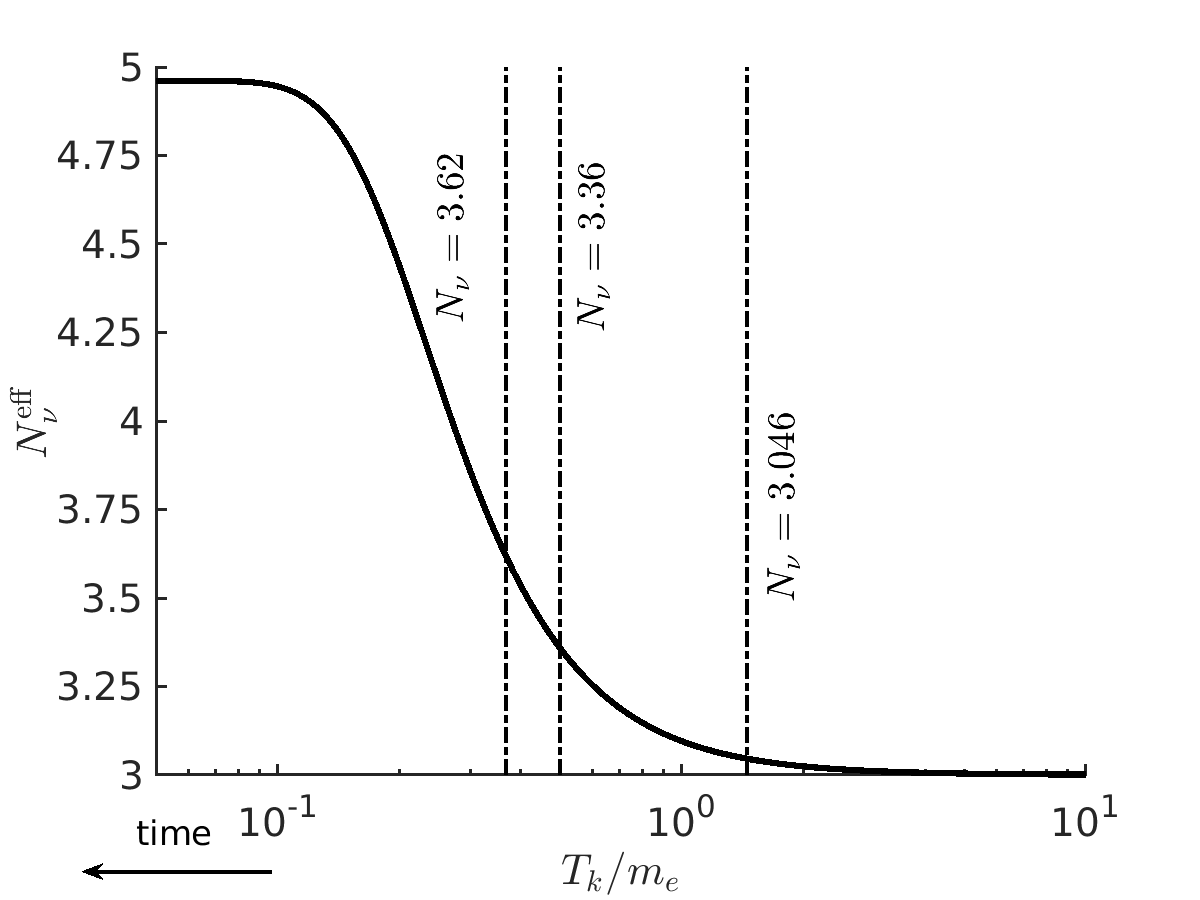
\includegraphics[width=0.90\linewidth]{04-birrell/ModelIndStudy/Figures/N_eff.pdf}}
\centerline{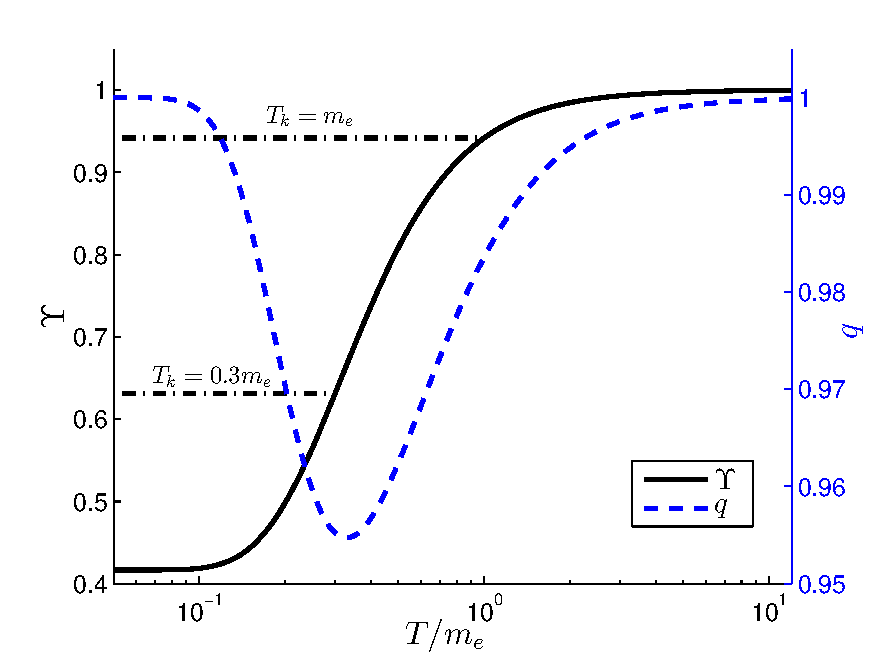
\includegraphics[width=0.90\linewidth]{04-birrell/ModelIndStudy/Figures/Upsilon_q.pdf}}
\caption{Dependence of effective number of neutrinos (top) and neutrino fugacity\index{fugacity!neutrino} (bottom) on the neutrino kinetic freeze-out temperature. We also show the evolution of the deceleration parameter through the freeze-out period (bottom)}
\label{fig:Tk_dependence}
\end{figure}
%%%%%%%%%%%%%%%%%%%%%%%%%%%%%%%%%%%%%%%
 In \rf{fig:Tk_dependence} we plot that dependence of $N^{\mathrm{eff}}_\nu$ and $\Upsilon$ on $T_k$ that is implied by these calculations. In particular, the fugacity evolves following the solid black curve in the bottom plot until it reaches the kinetic freeze-out temperature, at which point the neutrinos decouple and $\Upsilon$ remains constant thereafter, as shown in the dashed black curves for two sample values of $T_k$. 
 

 
Planck CMB\index{CMB} results~\cite{Planck:2013pxb} contain several fits based on different data sets which suggest that $N^{\mathrm{eff}}_\nu$ is in the range $3.30\pm 0.27$ to $3.62\pm0.25$ ($68\%$ confidence level). We note more recent Planck CMB analysis can be found in~\cite{Planck:2018vyg}. A numerical computation based on the Boltzmann equation with two body scattering~\cite{Mangano:2005cc} gives to $N_{\nu}^{\rm eff}=3.046$. These values are shown in the vertical lines in the left figure. The tension between the Planck results and theoretical reheating studies motivates our work.

%%%%%%%%%%%%%%%%%%%%%%%%%%%%%%%%%%%%%%%%%%%%%%%%%%%%%%%%%%%%%%%%%%%%
\para{Contribution to effective neutrino number from sub-eV mass sterile Particles}
Moving beyond neutrinos, we now study the effect on $N_\nu^{\text{eff}}$ of non-SM light weakly coupled particle species, referred to here as a sterile particles (SP)\index{sterile particles}. Such hypothetical SPs would behave as `dark radiation'~\cite{Steigman:2013yua} rather than cold dark matter and would therefore impact $N_\nu^{\text{eff}}$ in a similar manner to neutrinos, though potentially with a vastly different freeze-out temperature. This section is adapted from the work in \cite{Birrell:2014cja}.


The possibility that Goldstone bosons, one candidate for SPs, could be mistaken for a fractional contribution to cosmic neutrinos was identified in \cite{Weinberg:2013kea}. Another viable candidate for SPs are sterile neutrinos. It has been shown that three `new' right-handed neutrinos could fully account for the observed tension in the effective number of neutrinos\index{neutrino!effective number}, $N^{\text{eff}}_{\nu}$, if their freeze-out temperature is in the vicinity of the quark gluon plasma (QGP) phase transition~\cite{Anchordoqui:2011nh,Anchordoqui:2012qu}. If SPs originating in the QGP phase transition are interpreted as Goldstone bosons it would imply that in the deconfined phase there is an additional hidden symmetry, weakly broken at hadronization. For example, if this symmetry were to be part of the baryon conservation riddle, then we can expect that these Goldstone bosons will couple to particles with baryon number, and possibly only in the domain where the vacuum is modified from its present day condition. These considerations motivate study of the contribution to 
$N^{\text{eff}}_{\nu}$ of boson or fermion degrees of freedom (DoF) that froze out near to the QGP phase transformation. 

In this study we use the lattice-QCD derived QGP EoS from~\cite{Borsanyi:2013bia} to characterize the relation between $N^{\text{eff}}_{\nu}$ and the number of DoF that froze out at the time that the quark-gluon deconfined phase froze into hadrons near $T=150\MeV$. We work within the instantaneous freeze-out approximation, using the same reasoning that was applied to neutrinos, {\it i.e.\/}, we employ comoving entropy conservation\index{entropy!conservation} along with the facts that frozen-out particle species undergo temperature scaling with $1/a(t)$ and the remaining coupled particles undergo reheating at each $T\simeq m$ threshold, caused by a disappearing particle species transfer entropy into the remaining particles.



We denote by $S$ the conserved `comoving' entropy in a volume element $dV$, which scales with the factor $a(t)^3$. As we are no longer only considering just the neutrino freeze-out\index{neutrino!freeze-out}, here we employ the definition of the effective number of entropy DoF, $g_*^S$, given by
\begin{equation}
S=\frac{2\pi^2}{45}g^S_*T_\gamma^3 a^3\,.
\end{equation} 
For ideal fermion and boson gases
\begin{equation}
g_*^S=\!\!\!\!\sum_{i=\text{bosons}}\!\!\!\!g_i \left(\frac{T_i}{T_\gamma}\right)^3\!\!\!f_i^-+\frac{7}{8}\!\!\!\sum_{i=\text{fermions}}\!\!\!\! g_i \left(\frac{T_i}{T_\gamma}\right)^3\!\!\!f_i^+\,.
\end{equation}
The $g_i$ are degeneracies, $f_i^\pm$ are known functions, valued in $(0,1)$, that turn off the various species as the temperature drops below their mass; compare to the analogous Eqs. (2.3) and (2.4) in~\cite{Blennow:2012de}. 


%%%%%%%%%%%%%%%%%%%%%%%%%%%%%%%%%%%%%%%
\begin{figure}
\centerline{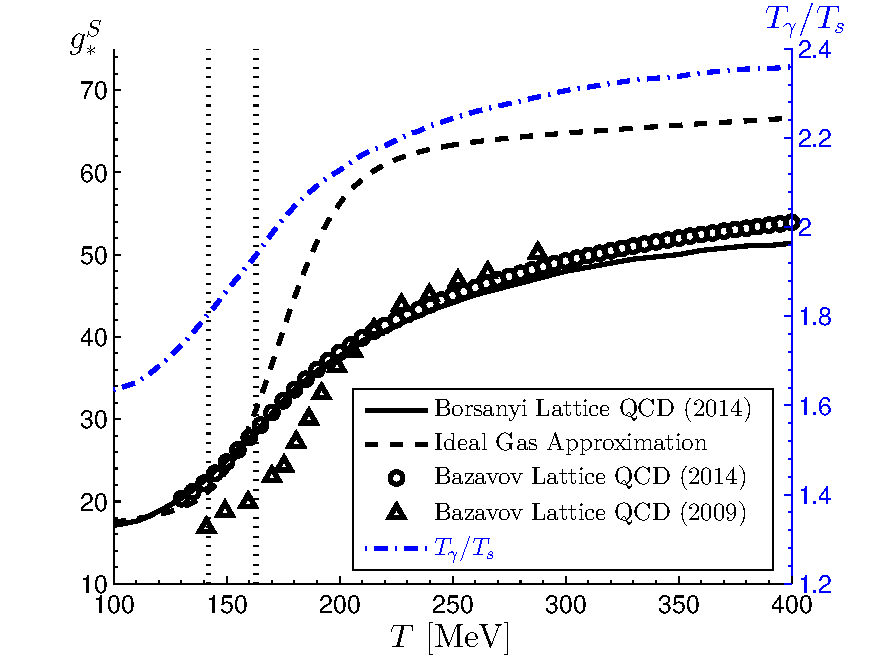
\includegraphics[width=0.9\linewidth]{04-birrell/ModelIndStudy/Figures/gS_T_ratio.pdf}}
\caption{Left axis: Effective number of entropy-DoF, including lattice QCD effects applying~\cite{Borsanyi:2013bia} (solid line) and~\cite{HotQCD:2014kol} (circles), compared to the earlier results~\cite{Bazavov:2009zn} (triangles) used by~\cite{Anchordoqui:2011nh}, and the ideal gas model of~\cite{Coleman:2003hs} (dashed line) as function of temperature $T$. Right axis: Photon to SP temperature ratio, $T_\gamma/T_s$, as a function of SP decoupling temperature (dash-dotted (blue) line). The vertical dotted lines at $T=142$ and 163 MeV delimit the QGP transformation region. \cccite{Birrell:2014cja}\label{fig:gS}}
 \end{figure}
%%%%%%%%%%%%%%%%%%%%%%%%%%%%%%%%%%%%%%%

Such a simple characterization does not hold in the vicinity of the QGP phase transformation where quark-hadron degrees of freedom are strongly coupled and the system must be studied using lattice QCD. A computation of $g_*^S$ that incorporates the lattice QCD results is shown in the solid line in Figure \ref{fig:gS} (left axis). Specifically, we used the table of entropy density\index{entropy!density} values through the QGP phase transition presented by Borsanyi et al.~\cite{Borsanyi:2013bia}, while circles show recent results from Bazavov et al.~\cite{HotQCD:2014kol}. This should be compared to the use of the ideal gas approximation from~\cite{Coleman:2003hs} together with the fit in~\cite{Wantz:2009it} to interpolate though the QGP phase transition and older (year 2009) lattice data from~\cite{Bazavov:2009zn} (triangles). The free gas approximation has a maximum error of $10\%$ in the QGP phase transition temperature range $T\simeq 150$\,MeV. The 2009 lattice data used in~\cite{Anchordoqui:2011nh} has a maximum error on the order of $25\%$ which leads to a non-negligible difference in the relation between freeze-out temperature and $N^{\text{eff}}_{\nu}$.

%%%%%%%%%%%%%%%%%%%%%%%%%%%%%%%%%%%%%%%
\begin{figure} 
\centerline{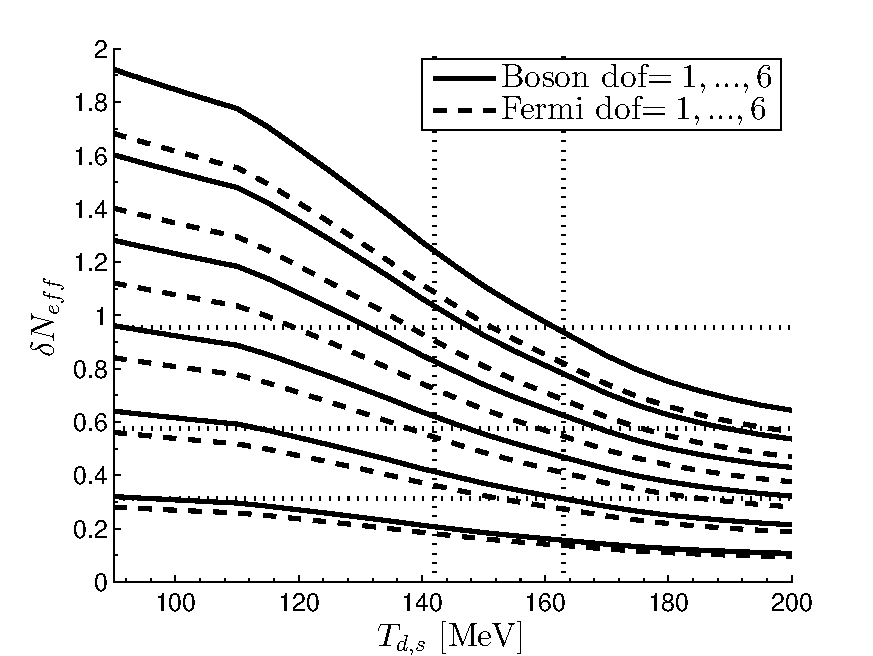
\includegraphics[width=0.9\linewidth]{04-birrell/ModelIndStudy/Figures/Neff_Td_combined.pdf}}
\caption{Solid lines: Increase in $\delta N_{\text{eff}}$ due to the effect of $1,\dots,6$ light sterile boson DoF ($g_s=1,\dots,6$, bottom to top curves) as a function of freeze-out temperature $T_{d,s}$. Dashed lines: Increase in $\delta N_{\text{eff}}$ due to the effect of $1,\dots,6$ light sterile fermion DoF ($g_s=7/8\times 1,\dots,7/8\times 6$, bottom to top curves) as a function of freeze-out temperature $T_{d,s}$. The horizontal dotted lines correspond to $\delta N_{\text{eff}}+0.046=0.36,0.62,1$. The vertical dotted lines show the reported range of QGP transformation temperatures $T_c=142-163\MeV$. \cccite{Birrell:2014cja}\label{fig:NeffTdZoom}}
\end{figure}
%%%%%%%%%%%%%%%%%%%%%%%%%%%%%%%%%%%%


Independent of their source, once the SPs decouple from the particle inventory at a photon temperature of $T_{d,s}$, a difference in their temperature from that of photons will build up during subsequent photon reheating periods, similarly to earlier computations. Conservation of entropy leads to a temperature ratio at $T_\gamma<T_{d,s}$, shown in the dot-dashed line in Figure \ref{fig:gS} (right axis), given by
\begin{equation}\label{eq:TRatio}
R_s\equiv T_{s}/T_{\gamma}=\left(\frac{g_*^S(T_\gamma)}{g_*^S(T_{d,s})}\right)^{1/3}\,.
\end{equation}
Evolving the Universe through neutrino freeze-out\index{neutrino!freeze-out}, if $T_s$ and $T_\gamma$ are the light SP and photon temperatures, both after $e^\pm$ annihilation, and $g_s$ is the number of DoF of the SPs normalized to bosons (i.e., for fermions it includes an additional factor of $7/8$) then this leads to the following change in the effective number of neutrinos\index{neutrino!effective number} in excess of the SM value:
\begin{equation}\label{Neff1}
\delta N_{\text{eff}}\equiv N^{\text{eff}}_{\nu}-3.046=\frac{4g_s}{7}\left(\frac{T_s}{R_s T_{\gamma}}\right)^4\,,
\end{equation}
where $3.046$ is the SM neutrino contribution. Using \req{eq:TRatio} we can rewrite $\delta N_{\text{eff}}$ as
\begin{equation}\label{eq:deltaN}
\delta N_{\text{eff}}=\frac{4g_s}{7R_\nu^4}\left(\frac{g_*^S(T_{\gamma})}{g_*^S(T_{d,s})}\right)^{4/3}\,,
\end{equation}
where $T_{d,s}$ is the decoupling temperature of the SP and $T_{\gamma}$ is any photon temperature in the regime $T_{\gamma}\ll m_e$. The SM particles remaining (in relevant amounts) at such $T_{\gamma}$ are photons and SM neutrinos, the latter with temperature $R_\nu T_{\gamma}$, and so $g_*^S(T_{\gamma})=2+7/8\times 6\times 4/11$ and (see also Eq.(2.7) in~\cite{Blennow:2012de})
\begin{align}\label{eq:deltaN2}
\delta N_{\text{eff}}\approx&g_s\left(\frac{7.06}{g_*^S(T_{d,s})}\right)^{4/3}\,.
\end{align}

In Figure \ref{fig:NeffTdZoom} we plot $\delta N_{\text{eff}}$ as a function of $T_{d,s}$ for $1,\dots,6$ boson (solid lines) and fermion (dashed lines) DoF. For a low decoupling temperature $T_{d,s}<100$\,MeV a single bose or fermi SP can help alleviate the observed tension in $N^{\text{eff}}_{\nu}$. Within the QGP hadronization\index{hadrons!hadronization} temperature range $T_c=142-163\MeV$ (marked by vertical dotted lines) we see that three boson degrees of freedom or four fermion degrees of freedom are the most likely cases to resolve the tension. If the SPs froze out in the QGP phase at $T_{d,s}\gg 163\MeV$ then a significantly larger number of SPs would be required. While such a scenario cannot be excluded, such a large number undiscovered weakly broken symmetries, or/and sterile neutrino-like particles, seems unlikely. Therefore we suggest that Figure \ref{fig:NeffTdZoom} pinpoints the QGP temperature range and below as the primary domain of interest for the freeze-out of a small to moderate number of hypothetical degrees of freedom, should these be responsible the excess in $N_\nu^{\text{eff}}$ above the SM value.

\subsection{Study of Neutrino Freeze-out using  the Boltzmann-Einstein Equation}\label{ch:param:studies}
%%%%%%%%%%%%%%%
In this section we remove the instantaneous freeze-out assumption  and present a more precise study of  neutrino freeze-out, i.e., we do not assume that the distribution is either in chemical or kinetic equilibrium or is free-streaming.
The required mathematical theory and numerical method is developed in Appendices \ref{ch:vol:forms}, \ref{ch:boltz:orthopoly}, and \ref{ch:coll:simp}.  Here we focus on the physical implications, in particular the dependence of the freeze-out process on natural constants. This allows us identify potential avenues by which the tension between observed and theoretical values of $N^{\mathrm{eff}}_\nu$ may be alleviated.   Our study also constrains the time and/or temperature variation of certain natural constants by comparing the results with measurements of $N_\nu^{\mathrm{eff}}$. Further details on this work can be found in \cite{Birrell:2014uka}. The topic of time variation of natural constants is a very active field with a long history; for a comprehensive review of this area, with which we make only slight contact,  see \cite{Uzan:2010pm}.  

%%%%%%%%%%%%%%%%%%%%%%%%%%%%%%%
\para{Neutrino Freeze-Out Temperature and Relaxation Time} 
To connect with the instantaneous freeze-out model from \rf{sec:model:ind}, we now give a definition of the kinetic freeze-out temperature that is applicable to the Boltzmann-Einstein equation model and use this to calculate the neutrino freeze-out temperature. Any such definition will be only approximate, as the freeze-out process is not a sharp transition.  Our definition is motivated in part the treatment in \cite{Kolb:1990vq}. 

We first define a characteristic length between scatterings. Using the formula \req{n:div}, we obtain the fractional rate of change of comoving particle number
\begin{align}
\frac{\frac{d}{dt}(a^3 n)}{a^3n}=\frac{g_\nu}{2\pi^2n}\int C[f]p^2/Edp\,.
\end{align}
Here we don't want the net change, but rather to count the number of interactions.  For that reason, we imagine that only one direction of the process is operational and define the relaxation rate\index{relaxation rate}
\begin{align}
\Gamma\equiv\frac{g_\nu}{2\pi^2n}T^2\int \tilde C[f]zdz\,,
\end{align}
where the one way collision is $\tilde C[f]$ is computed as in \req{coll} except with $F$ replaced by 
\begin{equation}
\tilde F=f_1(p_1)f_2(p_2)f^3(p_3)f^4(p_4)\,.
\end{equation}
If particle type $1$ also participates in the reverse of the reaction $1+2\rightarrow 3+4$ then a corresponding term for the reverse reaction must also be added.  The key difference is there is no minus sign; here we are counting reactions, not net particle number change.

Using the average velocity, which for (effectively massless) neutrinos is $\bar v=c=1$, we obtain what we call the scattering length\index{scattering length}
\begin{align}
L_\Gamma&\equiv\frac{\bar v}{\Gamma}=\frac{\int_0^\infty\frac{1}{\Upsilon^{-1}e^z+1}z^2dz}{\int_0^\infty \tilde C[f] z^2/E dz}\,.
\end{align}
This can be compared to the Hubble length $L_H=c/H$\index{Hubble length} and the temperature at which $L_\Gamma=L_H$ we call the freeze-out temperature\index{freeze-out temperature} for that reaction.  Figure \ref{fig:scatt_length} shows the scattering length and $L_H$ for various types of neutrino reactions.  The solid line corresponds to the annihilation process $e^+e^-\rightarrow \nu\bar\nu$, the dashed line corresponds to the scattering $\nu e^\pm\rightarrow \nu e^\pm$, and the dot-dashed line corresponds to the combination of all processes involving only neutrinos.  The freeze-out temperatures in MeV are given in Table \ref{table:freeze-out_temp}.

\begin{table}[ht]
\centering 
\begin{tabular}{|c|c|c|c|}
\hline
              & $e^+e^-\rightarrow \nu\bar\nu$ & $\nu e^\pm\rightarrow \nu e^\pm$ & $\nu$-only processes\\
\hline
$\nu_e$ &2.29 & 1.15&0.910\\
\hline
$\nu_{\mu,\tau}$ &3.83 & 1.78& 0.903\\
\hline
\end{tabular}
\caption{Freeze-out temperatures in MeV for electron neutrinos and for $\mu$,$\tau$ neutrinos.}
\label{table:freeze-out_temp}
\end{table}

%%%%%%%%%%%%%%%%%%%%%%%%%%%%%%%%%%%%%%%
\begin{figure} 
\centerline{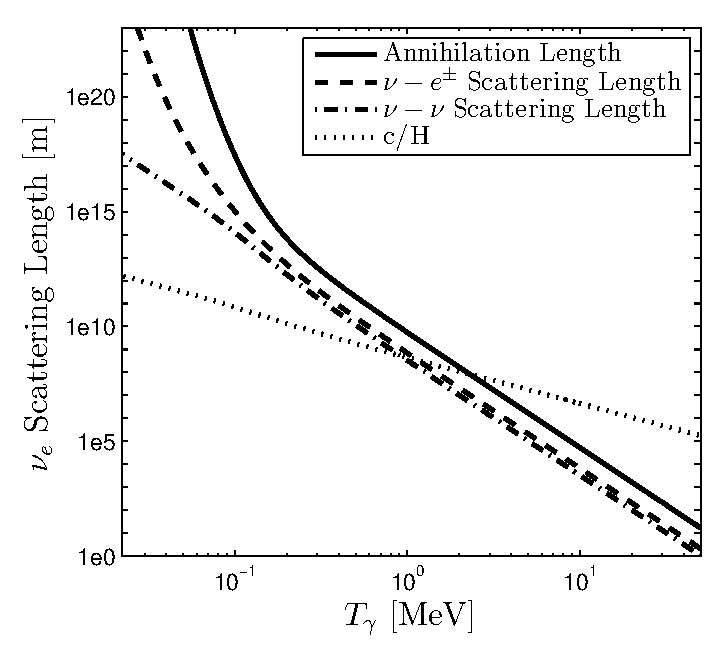
\includegraphics[height=6cm]{04-birrell/ParametricStudies/Figures/nu_e_scattering_length_eta_0_23.eps}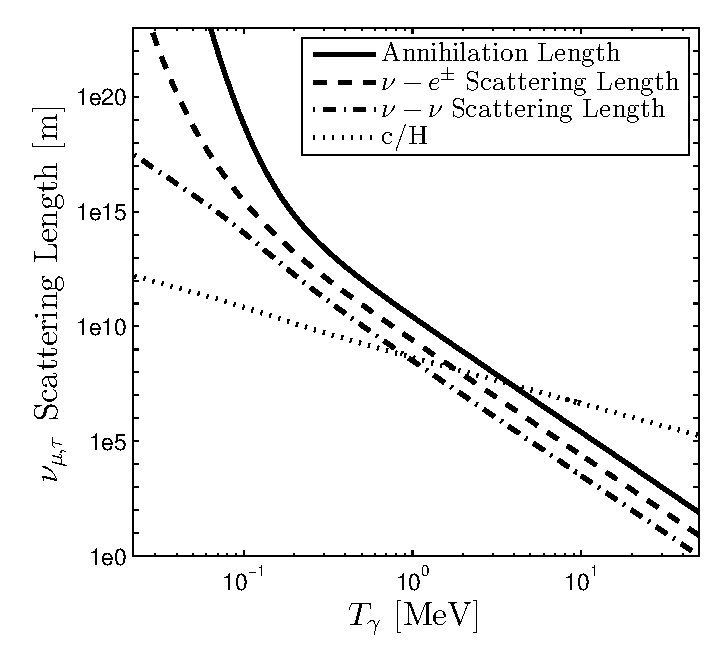
\includegraphics[height=6cm]{04-birrell/ParametricStudies/Figures/nu_mu_scattering_length_eta_0_23.eps}}
\caption{Comparison of Hubble parameter to neutrino scattering length for various types of PP-SM processes.  \cccite{Birrell:2014uka} }\label{fig:scatt_length}
\end{figure}
%%%%%%%%%%%%%%%%%%%%%%%%%%%%%%%%%%%%%%%


We now consider the the relaxation time\index{relaxation time} for a given reaction, defined by $\tau=1/\Gamma$.  Suppose we have a time interval $t_f>t_i$  and corresponding temperature interval $T_f<T_i$ during which there is no reheating and the Universe is radiation dominated.  Normalizing time so $t=0$ corresponds to the temperature $T_i$ we have
\begin{equation}\label{ch6:H_eq}
\dot a/a=-\dot T/T\,,\hspace{2mm} H=\frac{C}{2Ct+T_i^2}\propto T^2
\end{equation}
where $C$ is a constant that depends on the energy density and the Planck mass.  Its precise form will not be significant for us.  Note that \req{ch6:H_eq} implies
\begin{equation}
1/H(t)-1/H(0)=2t\,.
\end{equation}

At $T\gg m_e$, the rates for reactions under consideration from Tables \ref{table:nu:e:reac} and \ref{table:nu:mu:reac} scale as $\Gamma\propto T^5$.  Therefore, supposing $H(T_f)/\Gamma(T_f)=1$ (which occurs at $T_f=O(1\MeV)$ as seen in the above figures), at any time $t_f>t>t_i$ we find 
\begin{align}\label{relax_time}
\tau(t)/t=&\frac{2}{\Gamma(t)}\left(\frac{1}{H(t)}-\frac{1}{H(0)}\right)^{-1}=\frac{2T_f^5}{\Gamma(T_f)T^5}\left(\frac{T_f^2}{H(T_f)T^2}-\frac{T_f^2}{H(T_f)T_i^2}\right)^{-1}\\
=&\frac{2T_f^3}{T^3}\left(1-\frac{T^2}{T_i^2}\right)^{-1}\,.
\end{align}
Therefore, given any time $t_i<t_0<t_f$ we have
\begin{equation}\label{ch6:tau_eq}
\tau(t)<\tau(t_0)=\frac{2T_f^3}{T_0^3}\left(1-\frac{T_0^2}{T_i^2}\right)^{-1}\Delta t \text{ \,for all } t<t_0\,,
\end{equation}
where $\Delta t=t_0-t_i=t_0$.

 The first reheating period that precedes neutrino freeze-out is the disappearance of muons and pions around $O(100\MeV)$, as seen in Figure \ref{fig:energy_frac}, and so we let $T_i=100\MeV$. \req{ch6:tau_eq} is minimized at $T_0\approx 77.5\MeV$ at which point we have 
\begin{equation}
\tau(t)<10^{-5} \Delta t_0 \text{ for } t<t_0.
\end{equation}
This shows that the relaxation time during the period between $100\MeV$ and $77.5\MeV$ is at least five orders of magnitude smaller than the corresponding time interval.  Therefore the system has sufficient time to relax back to equilibrium after any potential non-equilibrium aspects developed during the reheating period.  Thus justifies our assumption that the neutrino distribution has the equilibrium Fermi Dirac form at $T=O(10 \MeV)$ when we begin our numerical simulation. This can also be demonstrated numerically in Figure \ref{fig:relax}, where we have initialized the system at $T_\gamma=12\MeV$ with a non-equilibrium distribution of $\mu$ and $\tau$ neutrinos, giving them $\Upsilon=0.9$, and let them evolve under the Boltzmann-Einstein equation.  We see that after approximately $10^{-3}$ seconds the system relaxes back to equilibrium, well before neutrino freeze-out near $t=1$s.

%%%%%%%%%%%%%%%%%%%%%%%%%%%%%%%%%%%%%%%
\begin{figure} 
%04-birrell/ParametricStudies/Figures/
\begin{minipage}{\linewidth}
\makebox[0.48\linewidth]%
{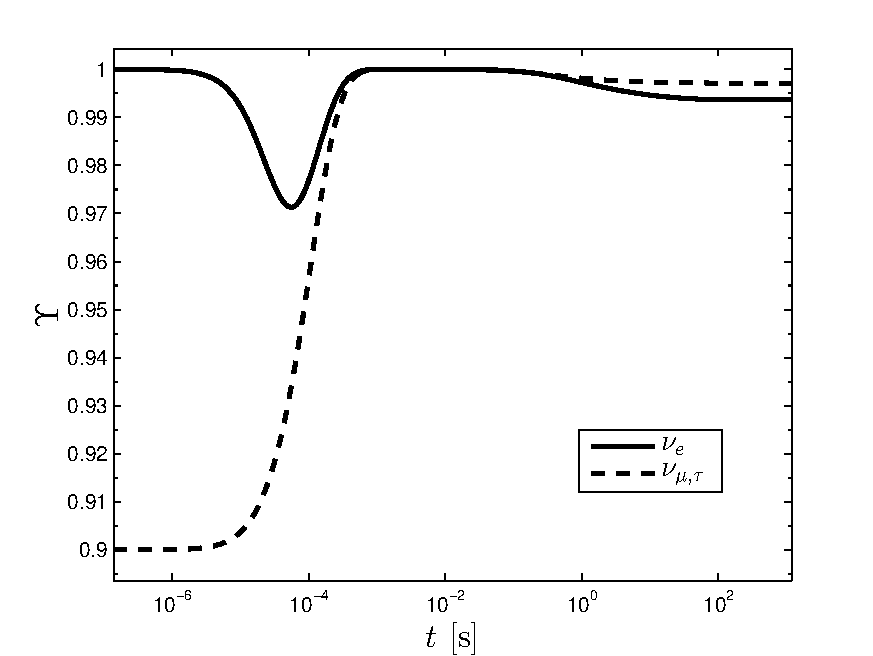
\includegraphics[height=5.5cm]{04-birrell/ParametricStudies/Figures/Ups_relax.eps}}
\makebox[0.48\linewidth]%
{\hspace{6mm}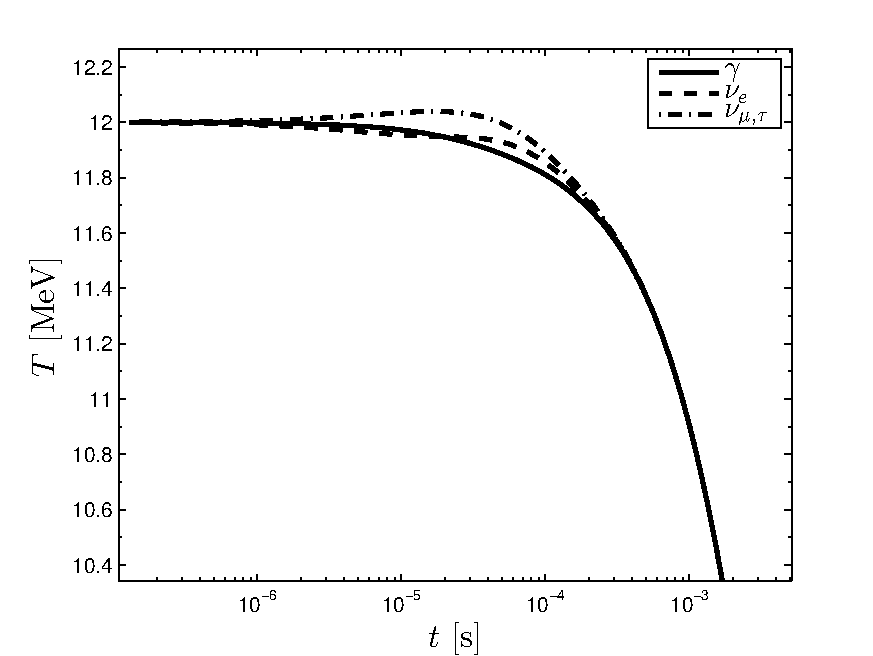
\includegraphics[height=5.5cm]{04-birrell/ParametricStudies/Figures/T_relax.eps}}
\end{minipage}
\caption{Starting at $12\MeV$, this figure shows the relaxation of a non-equilibrium $\mu,\tau$-neutrino distribution towards equilibrium. The fugacities are shown in the left frame while the temperatures are shown in the right frame}
\label{fig:relax}
 \end{figure}
%%%%%%%%%%%%%%%%%%%%%%%%%%%%%%%%%%%%%%%

%%%%%%%%%%%%%%%%%%%%%%%%%%%%%%%%%
\para{Dependence of effective neutrino number on PP-SM parameters}
%\label{sec:param_char}

Only two key PP-SM parameters  influence the effective number of neutrinos, this is the Weinberg angle and the generalized interaction strength $\eta$. We explore in the following how  $N_\nu^{\mathrm{eff}}$ depends on these parameters.

%\para{Weinberg Angle}
The Weinberg angle\index{Weinberg angle} is one of the key standard model parameters that impacts the neutrino freeze-out process.  More specifically, it is found in the matrix elements of weak force processes, including the reactions $e^+e^-\rightarrow \nu\bar\nu$ and $\nu e^\pm\rightarrow \nu e^\pm$ as found in Tables \ref{table:nu:e:reac} and \ref{table:nu:mu:reac}.  It is determined by the $SU(2)\times U(1)$ coupling constants $g$, $g^{'}$  by
\begin{equation}
\sin(\theta_W)=\frac{g^{'}}{\sqrt{g^2+(g^{'})^2}}\,.
\end{equation}
It is also related to the mass of the $W$ and $Z$ bosons and the Higgs vacuum expectation value $v$ by
\begin{equation}
M_Z=\frac{1}{2}\sqrt{g^2+(g^{'})^2}v\,,\hspace{2mm}  M_W=\frac{1}{2}gv\,,\hspace{2mm} \cos(\theta_W)=\frac{M_W}{M_Z}\,,
\end{equation}
as well as the electromagnetic coupling strength
\begin{equation}
e=2M_W\sin(\theta_W)/v=\frac{gg^{'}}{\sqrt{g^2+(g^{'})^2}}\,.
\end{equation}
It has a measured value in vacuum $\theta_W\approx 30^\circ$, giving $\sin(\theta_W)\approx 1/2$, but its value is not fixed within the Standard Model. For this reason, a time or temperature variation can be envisioned and this would have an observable impact on the neutrino freeze-out process, as measured by $N_\nu^{\mathrm{eff}}$.

In letting $\sin(\theta_W)$, and hence $g$ and $g^{'}$, vary we must fix the electromagnetic coupling $e$ so as not to impact sensitive cosmological observables such as Big Bang Nucleosynthesis.  

Fixing $v$, the smallest $M_W$ can become is when $\sin(\theta_W)=1$, yielding a reduction in $M_W$ by a factor of $2$.  This implies that $M_Z>M_W\gg |p|$ for neutrino momentum $p$ in the energy range of neutrino freeze-out, around $1\MeV$, even as we vary $\sin(\theta_W)$.  This approximation is inherent in the formulas for the matrix elements  in Tables  \ref{table:nu:e:reac} and \ref{table:nu:mu:reac} and continues to be valid here. We will characterize the dependence of $N_\nu^{\mathrm{eff}}$ on $\sin(\theta_W)$ in following, but first we identify the remaining parameter dependence in the Boltzmann-Einstein system

%%%%%%%%%%%%%%%%%%%%%%%%%%%%%%%%%%%%%
%\para{Interaction Strength} 
Beyond the Weinberg angle, the remaining dependence of the Boltzmann-Einstein system on dimensioned quantities during  neutrino freeze-out  can be combined in an overall interaction strength factor.   To show this, we now convert the system  to dimensionless form. Letting $m_e$ be the mass scale and $M_p/m_e^2$ be the time scale the Einstein equations take the form
\begin{equation}
H^2=\frac{\rho}{3}\,,\hspace{2mm}\dot\rho=-3H(\rho+P)\,.
\end{equation}
 Since $e^\pm$ are the only (effectively) massive particles in the system, by scaling all energies, momenta, energy densities, pressures, and temperatures by $m_e$ we have removed all scale dependent parameters from the Einstein equations.  The Boltzmann-Einstein equation becomes
\begin{equation}\label{eta_def}
\partial_tf-pH\partial_pf=\eta\frac{C[f]}{E}\,,\hspace{2mm}\eta\equiv M_p m_e^3G_F^2\,,
\end{equation}
where we have also factored out of $C[f]$ the $G_F^2$ term that is common to all of the neutrino interaction matrix elements. 

Aside from the $\theta_W$ dependence of the matrix elements seen in Tables \ref{table:nu:e:reac} and \ref{table:nu:mu:reac}, the complete dependence on natural constants  is now contained in a single dimensionless neutrino interaction strength parameter\index{neutrino interaction strength} $\eta$ with the vacuum present day value,
\begin{equation}\label{eta0_def}
\eta_0\equiv \left.M_p m_e^3 G_F^2\right|_0  \approx 0.04421\, .
\end{equation}

%%%%%%%%%%%%%%%%%%%%%%%%%%%%%%%%%%%
\para{Impact of QED Corrections to Equation of State}\index{QED!Corrections EoS}
%\label{app:QED_corr} 
At the time of neutrino freeze-out, the universe is at sufficiently high temperature for photons and $e^\pm$ to be in chemical and kinetic equilibrium.  The temperature is also sufficiently high for QED corrections to the photon and $e^\pm$ equation of state to be non-negligible.  Therefore, in our study here we use the results given in \cite{Heckler:1994tv,Mangano:2001iu} to include these in our computation by modifying the combined photon, $e^\pm$ equation of state
\begin{align}
P=P^0+P^{int},\hspace{2mm} \rho=-P+T\frac{dP}{dT}\,,
\end{align}
where
\begin{align}
P^{int}=&-\frac{1}{2\pi^2}\int_0^\infty\left[\frac{k^2}{E_k}\frac{\delta m_e^2}{e^{E_k/T}+1}+\frac{k}{2}\frac{\delta m_\gamma^2}{e^{k/T}-1}\right]dk\,,\hspace{2mm} E_k=\sqrt{k^2+m_e^2}\,,\\
\delta m_e^2=&\frac{2\pi\alpha^2}{3}+\frac{4\alpha}{\pi}\int_0^\infty \frac{k^2}{E_k}\frac{1}{e^{E_k/T}+1}dk\,,\hspace{2mm} \delta m_\gamma^2=\frac{8\alpha}{\pi}\int_0^\infty \frac{k^2}{E_k}\frac{1}{e^{E_k/T}+1}dk\,,
\end{align}
and $P^0$ is the pressure of a non-interacting gas of photons and $e^\pm$ in chemical equilibrium.

%%%%%%%%%%%%%%%%%%%%%%%%%%%%%%%%%%%%
\para{Freeze-out T and effective neutrino number dependence on PP-SM}
We now present the  dependence of the effective number of neutrinos, $N_\nu^{\mathrm{eff}}$, on  the SM parameters   $\sin^2(\theta_W)$ and $\eta$, as computed using the Boltzmann-Einstein equation method developed in Appendices \ref{ch:vol:forms}, \ref{ch:boltz:orthopoly}, and \ref{ch:coll:simp}. These results are shown in  Figure \ref{N_nu_params}, presented as a function of  Weinberg angle $\sin^2(\theta_W) $ for $\eta/\eta_0=1,2,5,10$. The effects of an increase in both parameters above the vacuum values generate a significant increase in  $N_\nu^{\mathrm{eff}}\to 3.5$.  The dependence of freeze-out temperatures on $\eta$ is shown in Figure \ref{fig:freezeoutT_eta} and the dependence on Weinberg angle is shown in Figure \ref{fig:freezeoutT_B}. The present day vacuum value of Weinberg angle puts the $\nu_\mu,\nu_\tau$ freeze-out temperature, seen in the right pane of Figure \ref{fig:freezeoutT_B},  near its maximum value.  This is why a comparatively large change in $\sin^2(\theta_W)$ is needed to produce a change in $N_\nu^{\mathrm{eff}}$ for $\sin^2(\theta_W)\approx0.23$.  
 
%%%%%%%%%%%%%%%%%%%%
\begin{figure}
\centerline{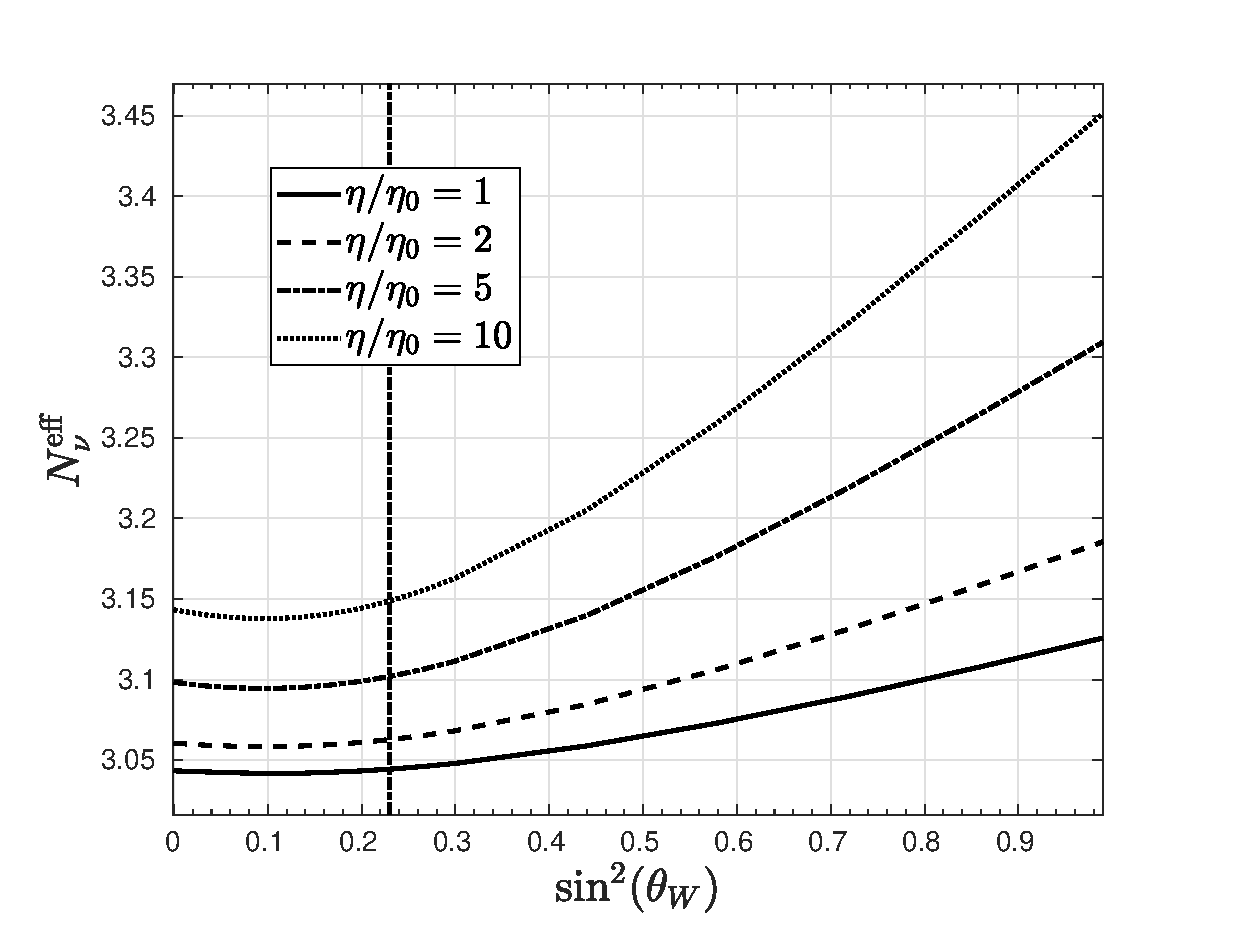
\includegraphics[width=0.90\columnwidth]{04-birrell/ParametricStudies/Figures/N_eff2.eps}}
\caption{Change in effective number of neutrinos  $N_\nu^{\mathrm{eff}}$ as a function of Weinberg angle for  several values of $\eta/\eta_0=1,2,5,10$. Vertical line is $\sin^2(\theta_W)=0.23$. Adapted from \cite{Birrell:2014uka}}
\label{N_nu_params}  
 \end{figure}
%%%%%%%%%%%%%%%%%%%%

We performed a least squares fit of $N_\nu^{\mathrm{eff}}$ over the range $0\leq \sin^2(\theta_W)\leq 1$, $1\leq \eta/\eta_0\leq 10$ shown in figure \ref{N_nu_params}, obtaining a result with relative error less than $0.2\%$,
\begin{align}
N_\nu^{\mathrm{eff}}=&3.003-0.095\sin^2(\theta_W) +0.222\sin^4(\theta_W ) -0.164\sin^6(\theta_W )\notag\\
+&\sqrt{\frac{\eta}{\eta_0}}\left(0.043+0.011\sin^2(\theta_W) +0.103\sin^4(\theta_W)\right)\,.
\end{align}
$N_\nu^{\mathrm{eff}}$ is monotonically increasing in $\eta/\eta_0$ with dominant behavior  scaling as $\sqrt{ \eta/\eta_0}$. Monotonicity is to be expected, as increasing $\eta$ decreases the freeze-out temperature and the longer neutrinos are able to remain coupled to $e^\pm$, the more energy and entropy from annihilation is transferred to neutrinos.

%%%%%%%%%%%%%%%%%%%%%%%%%%%%%%%%%%%%%%%
\begin{figure}
\centerline{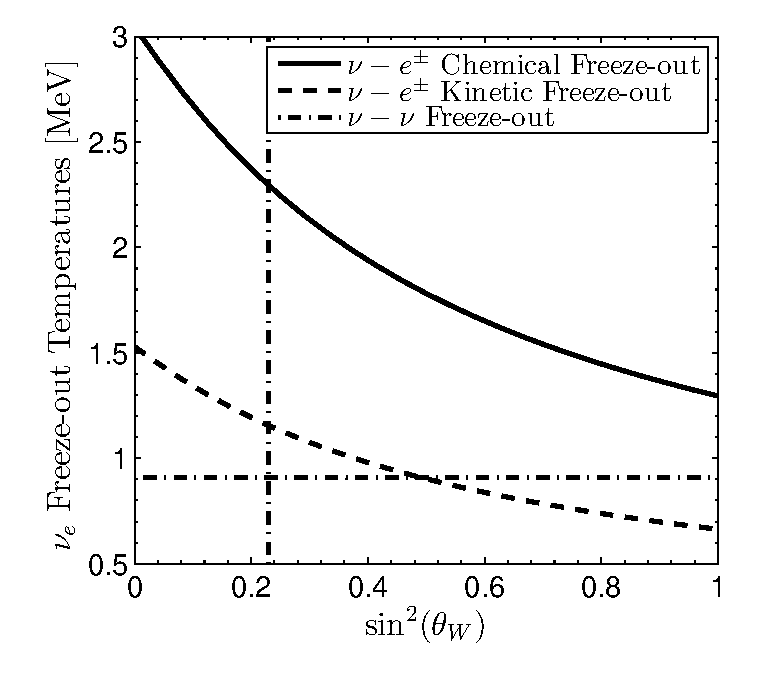
\includegraphics[height=6.3cm]{04-birrell/ParametricStudies/Figures/nu_e_freezeout.eps}\hspace{5mm}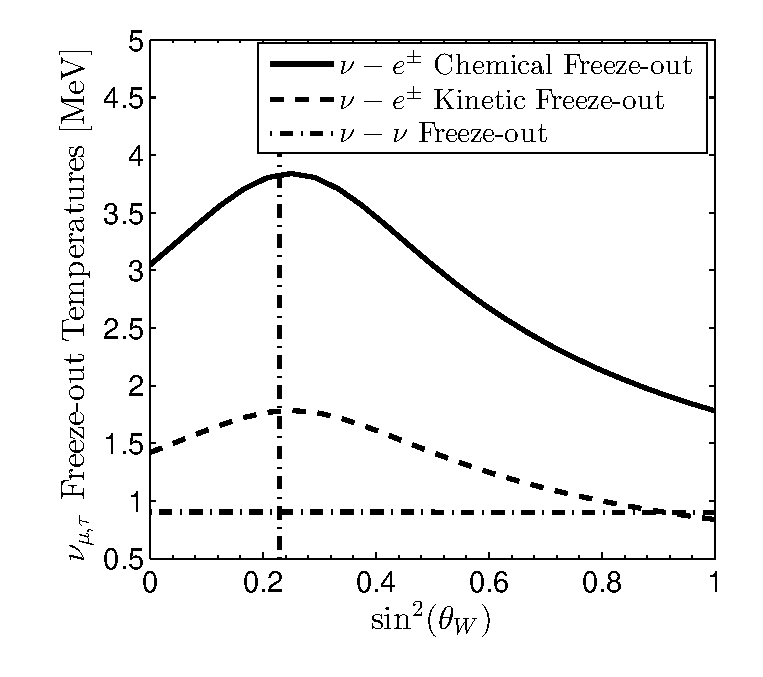
\includegraphics[height=6.3cm]{04-birrell/ParametricStudies/Figures/nu_mu_freezeout.eps}}
\caption{Freeze-out temperatures for electron neutrinos (left) and $\mu$, $\tau$ neutrinos (right) for various types of processes, as functions of Weinberg angle. Vertical line is $\sin^2(\theta_W)=0.23$. \cccite{Birrell:2014uka}}
\label{fig:freezeoutT_B}
 \end{figure}
%%%%%%%%%%%%%%%%%%%%%%%%%%%%%%%%%%%%%%%

%%%%%%%%%%%%%%%%%%%%%%%%%%%%%%%%%%%%%%%
\begin{figure}
\centerline{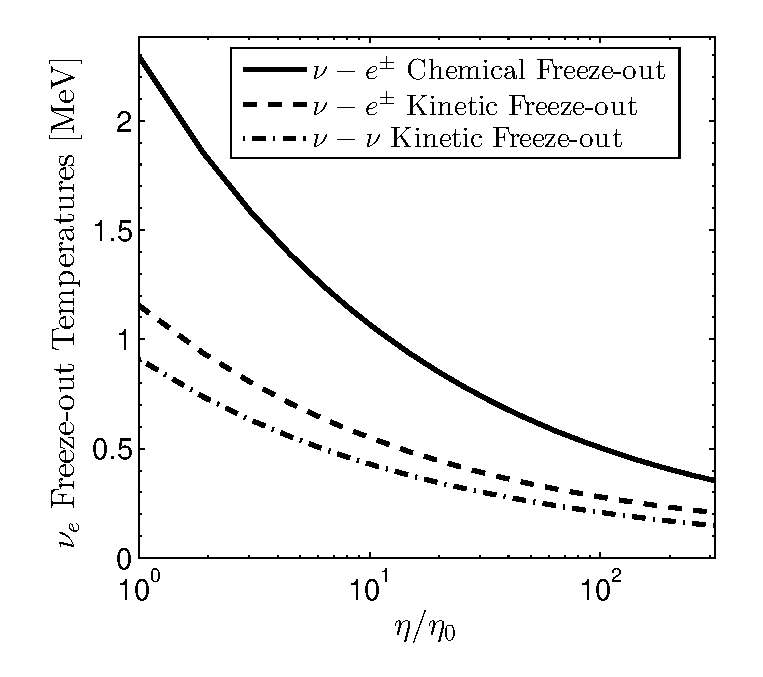
\includegraphics[height=6.3cm]{04-birrell/ParametricStudies/Figures/nu_e_freezeout_GF.eps}\hspace{5mm}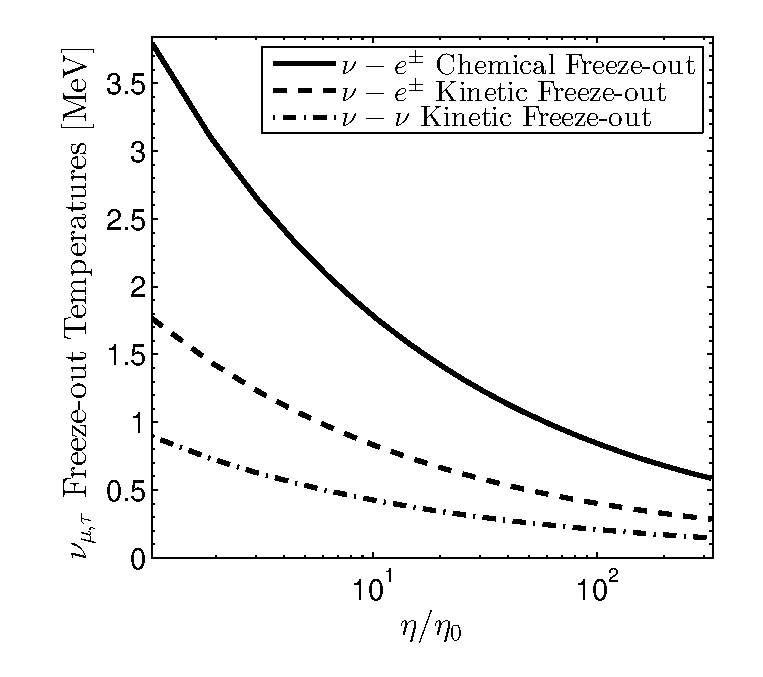
\includegraphics[height=6.3cm]{04-birrell/ParametricStudies/Figures/nu_mu_freezeout_GF.eps}}
\caption{Freeze-out temperatures for electron neutrinos (left) and $\mu$, $\tau$ neutrinos (right) for various types of processes, as functions of interaction strength. \cccite{Birrell:2014uka}}
\label{fig:freezeoutT_eta}
 \end{figure}
%%%%%%%%%%%%%%%%%%%%%%%%%%%%%%%%%%%%%%%



We complement this with fits to the photon to neutrino temperature ratios $ T_\gamma / T_{\nu_e}$, $T_\gamma / T_{\nu_\mu}= T_\gamma / T_{\nu_\tau} $, and the neutrino fugacities, $\Upsilon_{\nu_e}, \Upsilon_{\nu_\mu}=\Upsilon_{\nu_\tau}$, again with relative error less than $0.2\%$,  
\begin{align}
\frac{T_\gamma}{T_{\nu_\mu}}=&1.401+0.015x-0.040x^2+0.029x^3-0.0065y+0.0040xy-0.017x^2y\,, \notag\\
\Upsilon_{\nu_e}=&1.001+0.011x-0.024x^2+0.013x^3-0.005y-0.016xy+0.0006x^2y\,,\notag\\ 
\frac{T_\gamma}{T_{\nu_e}}=&1.401+0.015x-0.034x^2+0.021x^3-0.0066y-0.015xy-0.0045x^2y\,,\notag\\
\Upsilon_{\nu_\mu}=&1.001+0.011x-0.032x^2+0.023x^3-0.0052y+0.0057xy-0.014x^2y\,,
\end{align}
where
\begin{equation}%{align}
x\equiv \sin^2(\theta_W)\, ,\qquad
y\equiv  \sqrt{\frac{\eta}{\eta_0}}\,.
\end{equation}%{align}

%%%%%%%%%%%%%%%%%%%%
\begin{figure}
\centerline{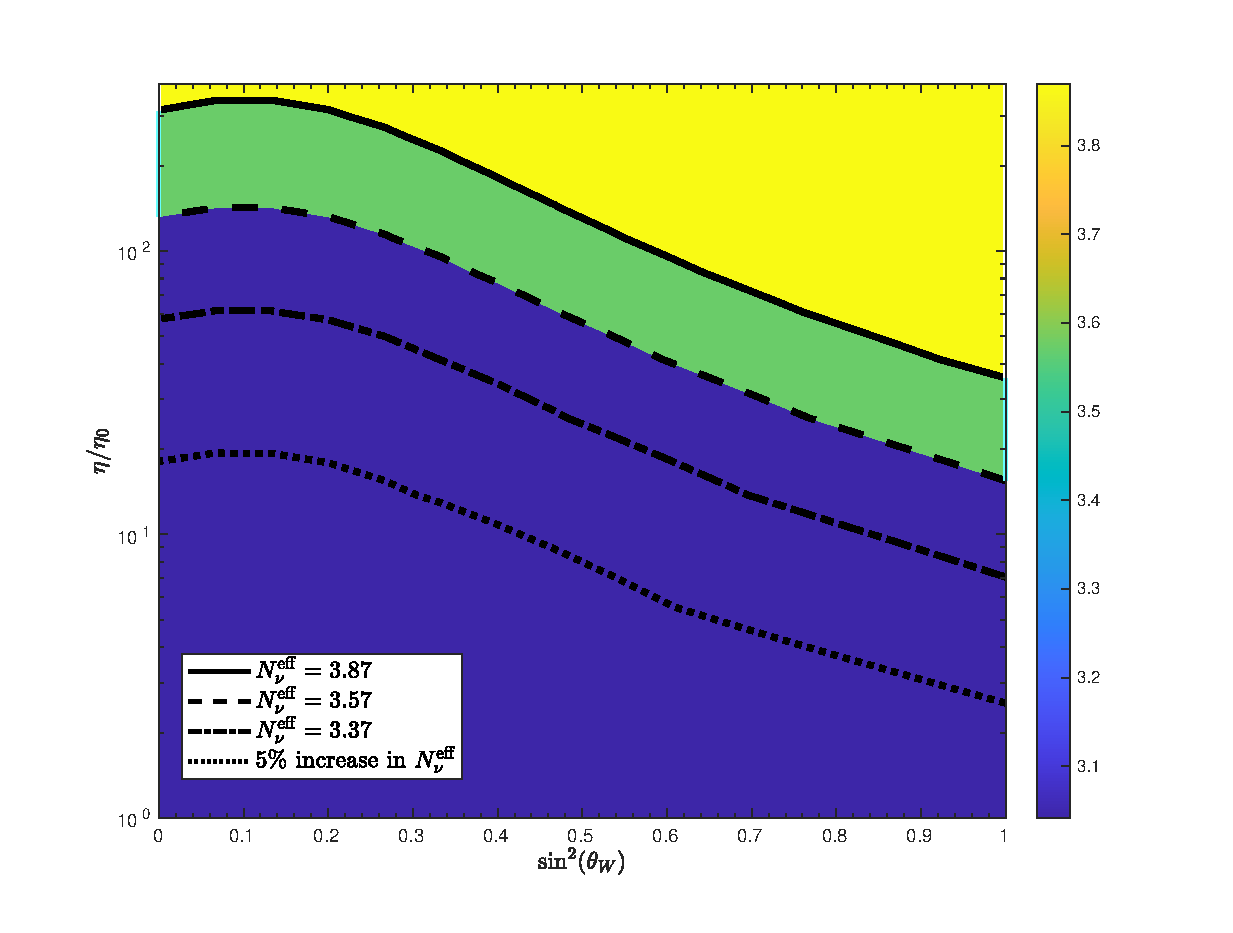
\includegraphics[width=0.9\columnwidth]{04-birrell/ParametricStudies/Figures/region_plot_legend.eps}
}
\caption{$N_\nu^{\mathrm{eff}}$ bounds in the $\eta/\eta_0, \sin^2(\theta_W)$ plane. Blue for $N_\nu^{\mathrm{eff}}\in (3.03,3.57)$ corresponding to Ref.~\cite{Planck:2013pxb} CMB+BAO analysis and green extends the region to $N_\nu^{\mathrm{eff}}<3.87$ i.e. to CMB+$H_0$. Dot-dashed line delimits the 1 standard-deviation lower boundary of the second analysis. Adapted from \cite{Birrell:2014uka}}
\label{N_nu_domain}
 \end{figure}
%%%%%%%%%%%%%%%%%%%%

The bounds on $N_\nu^{\mathrm{eff}}$ from the Planck analysis \cite{Planck:2013pxb} can be  used to constrain time or temperature variation of $\sin^2(\theta_W)$ and $\eta$.  
In  Figure \ref{N_nu_domain} the blue region shows the combined range of  variation of natural constants  compatible with CMB+BAO and the green region shows  the extension in the range of  variation of  natural constants for CMB+$H_0$, both at a $68\%$ confidence level. The dot-dashed line within the blue region delimits   this latter domain. The dotted line shows the limit of a 5\% change in $N_\nu^{\mathrm{eff}}$.    Any increase in  $\eta/\eta_0$ and/or $\sin^2(\theta_W)$ moves the value of $N_\nu^{\mathrm{eff}}$ into the domain favored by current experimental results.

%%%%%%%%%%%%%%%%%%%
We have omitted here a discussion of flavor neutrino oscillations. If it weren't for the differences between the matrix elements for the interactions between $e^\pm$ and $\nu_e$ on one hand and $e^\pm$ and $\nu_\mu,\nu_\tau$ on the other, oscillations would have no effect on the flow of entropy into neutrinos and hence no effect on $N_\nu^{\mathrm{eff}}$, but these differences do lead to a modification of $N_\nu^{\mathrm{eff}}$.  In \cite{Mangano:2005cc} the impact of oscillations on neutrino freeze-out for the present day measured values of $\theta_W$ and $\eta$ was investigated.  It was found  that while oscillations redistributed energy amongst the neutrino flavors, the impact on $N_\nu^{\mathrm{eff}}$ was negligible. We have neglected oscillations in our study.

%%%%%%%%%%%%%%%%%%%%%%%%%%%%%%%%%%%%
\para{Primordial Variation of Natural Constants}
We end our study of neutrino freeze-out by exploring what neutrino decoupling in the early Universe can tell us about the values of natural constants when the Universe was about one second old and at an ambient temperature near to 1 MeV (11.6 billion degrees K). Our results were presented assuming that the Universe contains no other effectively massless particles but the three left handed neutrinos and  three corresponding right handed anti-neutrinos. 

In \rf{N_nu_params} we see that, near  the present day value of the Weinberg angle  $\sin^2(\theta_W)\simeq 0.23$, the effect of changing $\sin^2(\theta_W)$ on the decoupling of neutrinos is small. The dominant variance is due to the change  in the coupling strength $\eta/\eta_0$, \req{eta_def}  and \req{eta0_def}. The dotted line in  Figure \ref{N_nu_domain} shows that in order to achieve a change in $N_\nu^{\mathrm{eff}}$ at the level of up to 5\%, i.e., $N_\nu^{\mathrm{eff}}\lesssim 3.2 $,   $\eta/\eta_0$ must change significantly, e.g.,  increasing by an order of magnitude.

We would like to better understand whether, in the primordial Universe, $\eta$ could be significantly (i.e., an order
of magnitude) different from the current value. We explore the rationale governing this
hypothesis by considering the natural constants  contributing to $\eta$ and their required
modification:
\begin{itemize}
\item
In models of emergent gravity we can imagine a `melting' of gravity in the hot primordial
Universe, just like we see the vacuum structure and quark confinement melt. Conversely, and
perhaps more attractive in light of the present day interest in the so called Hubble-tension, there could be
present-era weakening of gravity which would allow the Universe expansion to accelerate and more
generally could also modify the dark energy input into Universe dynamics. Whether such a
variable gravity model can be realized will be a topic for future consideration. Considering
that  $\eta\propto M_p\propto G_N^{-1/2}$ the value of $\eta$ will change in the opposite to the
strength of gravity: An order magnitude change in $\eta$ at the time of neutrino decoupling
translates into two orders of magnitude (inverse) change in the strength of gravity. One would
not think this is a possible scenario but a change in gravity strength by a less extreme factor
could be imagined.
\item
Compared to all other elementary particles the electron mass has an unusually low value. This
could imply a more complicated mass origin of the electron when compared to other elementary
particles which are drawing their mass by the minimal coupling from the Higgs field.  We studied
  a strong field mechanism for electron mass melting recently~\cite{Evans:2019zyk}. Since
$\eta\propto m_e^3$, electron mass would need to change at the time of decoupling of neutrinos by
`only' a factor 2.15 to create an order of magnitude impact on $\eta$.
\item
A modification by `only' a factor of 1.8  in the vacuum  expectation value (VEV) of the Higgs field
$v_0\simeq 246$ GeV  controlling the weak interaction coupling $G_\mathrm{F}\propto 1/v^4$ would
suffice to alter $\eta$ by an order of magnitude. However, if we allow electron mass to be also
Higgs controlled,  three powers of $v$ would cancel and a change in $v$ by an order of magnitude
near to $T\simeq m_e$ would be required. In either case, given our good understanding of the
standard model of particle physics  we do not believe that the  VEV of the Higgs field could be
impacted by the conditions prevailing at the time of neutrino decoupling.
\end{itemize}
To summarize: Gravity is an effective theory poorly understood at a fundamental level. Electron
mass is `anomalously' small and has a scale below the temperature scale of neutrino decoupling.
Thus both could potentially  be the cause of a substantial change in $\eta$. On the other hand the Higgs VEV seems
immutable at neutrino decoupling, considering the relevant scale being 500,000 times greater.

One could argue that time dependence of  $\sin^2(\theta_W)$ remains without a theoretical
motivation, mainly so since in SU(5) model unifying  quarks and leptons a value
$\sin^2(\theta_W)=1/4$  appears. Since this model has been discredited by baryon stability, any
value of $\sin^2(\theta_W)$ seems possible at time of neutrino decoupling, as there is no known
rational for the observed   mixing value of $\sin^2(\theta_W)$.



\subsection{Neutrinos Today}\label{ch:nu:today}
%%%%%%%%%%%%%%%%%%%%%%%%%%%%%%%%%%%%%%%%%%%%%%
Experimental detection of the cosmic background neutrinos is a challenge of great interest \cite{Stodolsky:1974aq,Cabibbo:1982bb,Shvartsman,Langacker:1982ih,Smith:1983jj,Ferreras:1995wf,Hagmann:1999kf,Duda:2001hd,Gelmini:2004hg,Ringwald:2009bg,Liao:2012wb,Hedman:2013hha}. With the  recently proposed PTOLEMY experiment, which aims to detect relic  electron-neutrino capture by tritium \cite{Betts:2013uya}, the characterization of the relic neutrino background is increasingly relevant.  Using our  characterization of the neutrino distribution after freeze-out and the subsequent free-streaming dynamics from Section  \ref{sec:model:ind} and \cite{Birrell:2012gg}, we lay groundwork for a characterization of the present day relic neutrino spectrum, which we explore  from the  perspective of an observer moving relative to the neutrino background, including the dependence on neutrino mass and effecitve number of neuntrinos, $N_\nu^{\mathrm{eff}}$. Beyond consideration of the observable neutrino distributions, we evaluate the ${\cal O}(G_F^2)$ mechanical drag force acting on the moving observer. This section is adapted from the work in \cite{Birrell:2014qna}.

%%%%%%%%%%%%%%%%%
\para{Neutrino Distribution in a Moving Frame}
The neutrino background and the cosmic microwave background (CMB) were in equilibrium until decoupling (called freeze-out) at $T_k\simeq {\cal O}{\rm (MeV)}$, hence one surmises that an observer would have the same relative velocity relative to the relic neutrino background  as with CMB. As a particular example in considering the spectrum, we present in more detail the case of an observer comoving with  Earth velocity $v_\oplus=300$\,km/s relative to the CMB,  modulated by orbital velocity ($\pm29.8$\,km/s).  We will write velocities in units of $c$, though our specific results will be presented in km/s.

In the cosmological setting, for $T<T_k$ the neutrino spectrum evolves according to the well known Fermi-Dirac-Einstein-Vlasov (FDEV) free-streaming  distribution~\cite{Langacker:1982ih,Choquet-Bruhat:2009xil,Wong:2011ip,Birrell:2012gg}.  By casting it in a relativistically invariant form we can then make a transformation to the rest frame of an observer moving with relative velocity $v_{\text{rel}}$ and obtain
\begin{align}\label{neutrino_dist_B}
f(p^\mu)=&\frac{1}{\Upsilon^{-1} e^{\sqrt{(p^\mu U_\mu)^2-m_\nu^2}/T_\nu}+1}\,.
\end{align}
The 4-vector characterizing the rest frame of the neutrino FDEV distribution is
\begin{equation}\label{4_vel}
U^\mu=(\gamma,0,0,v_{\text{rel}}\gamma)\,,\hspace{2mm} \gamma={1}/{\sqrt{1-v_{\text{rel}}^2}}\,,
\end{equation} 
where we have chosen coordinates so that the relative motion is in the $z$-direction. 

The neutrino effective temperature $T_\nu(t)= T_k\,(a(t_k)/a(t))$ is the scale-shifted freeze-out temperature $T_k$. Here $a(t)$ is the cosmological scale factor where $\dot a(t)/a(t)\equiv H$ is the observable Hubble parameter. $\Upsilon$ is the  fugacity factor, here describing the underpopulation of neutrino phase space that was frozen into the neutrino FDEV distribution in the process of decoupling from the $e^\pm,\gamma$-QED background  plasma.

There are several available bounds on neutrino masses. Neutrino energy and pressure components are important before photon freeze-out and thus $m_\nu$ impacts Universe dynamics. The analysis of CMB data alone leads to $\sum_i m_\nu^i<0.66$eV ($i=e,\mu,\tau$) and including Baryon Acoustic Oscillation (BAO) gives $\sum m_\nu<0.23$eV~\cite{Planck:2013pxb}.  {\small PLANCK CMB} with lensing observations~\cite{Battye:2013xqa} lead to  $\sum m_{\nu}=0.32\pm0.081$ eV. Upper bounds have been placed on the electron neutrino mass in direct laboratory measurements  $m_{\bar\nu_e}<2.05$eV~\cite{Troitsk:2011cvm}.   In the subsequent analysis we will focus on the neutrino mass range $0.05$eV to $2$eV in order to show that direct measurement sensitivity allows the exploration of a wide mass range. 

 The relations in \req{modindeq1}\,-\,\req{modindeq3}, see also~\cite{Birrell:2012gg}, determine $T_\nu/T_\gamma$ and  $\Upsilon$ in terms of the measured  value of  $N_\nu^{\mathrm{eff}}$ under the assumption of a strictly SM-particle inventory.  In the following we treat $N_\nu^{\mathrm{eff}}$  as a variable model parameter and use the above mentioned relations to characterize our results in terms of $N_\nu^{\mathrm{eff}}$.

%%%%%%%%%%%%%%%%%%%%%%%
\para{Velocity, Energy, and Wavelength Distributions}
Using \req{neutrino_dist_B}, the normalized FDEV velocity distribution for an observer in relative motion has the form
\begin{align} \label{fvdistrib}
&f_v=\frac{g_\nu}{n_\nu 4\pi^2}\!\!\!\int_0^\pi \!\!\!\!\frac{ p^2dp/dv\sin(\phi) d\phi}{\Upsilon^{-1}e^{\sqrt{( E-v_{\text{rel}} p \cos(\phi))^2\gamma^2-m_\nu^2}/T_\nu}+1}\,,\notag\\
&p(v)=\frac{m_\nu v}{\sqrt{1-v^2}}\,,\qquad \frac{dp}{dv}=\frac{m_\nu}{(1-v^2)^{3/2}}\,.
\end{align}
The normalization $n_\nu$ depends on $N_\nu^{\mathrm{eff}}$ but not on $m_\nu$ since decoupling occurred at $T_k\gg m_\nu$. For each neutrino flavor (all flavors are equilibrated by oscillations) we have, per neutrino or antineutrino and at non-relativistic relative velocity,
\begin{equation}\label{nnu}
n_\nu=[-0.3517(\delta N_\nu^{\mathrm{eff}})^2+6.717\delta N_\nu^{\mathrm{eff}}+56.06]\,{\rm cm}^{-3}
\end{equation}
($\delta N_\nu^{\mathrm{eff}}\equiv N_\nu^{\mathrm{eff}}-3$), compare to Eq.(55) in Ref.~\cite{Birrell:2012gg}.

We show $f_v$ in Figure \ref{fig:rel_v_dist_300}   for several values of the neutrino mass, $v_{\text{rel}}=300$ km/s, and $N_\nu^{\mathrm{eff}}=3.046$ (solid lines) and $N_\nu^{\mathrm{eff}}=3.62$ (dashed lines). As expected, the lighter the neutrino, the more $f_v$  is weighted towards higher velocities with the velocity becoming visibly peaked about $v_{\text{rel}}$ for $m_\nu=2$ eV. 
%%%%%%%%%%%%%%%%%%%%%%%%%%%%%%%%%%%%%%%

%%%%%%%%%%%%%%%%%%%%%%%%%%%%%%%%%%%%%%%
\begin{figure}
\centerline{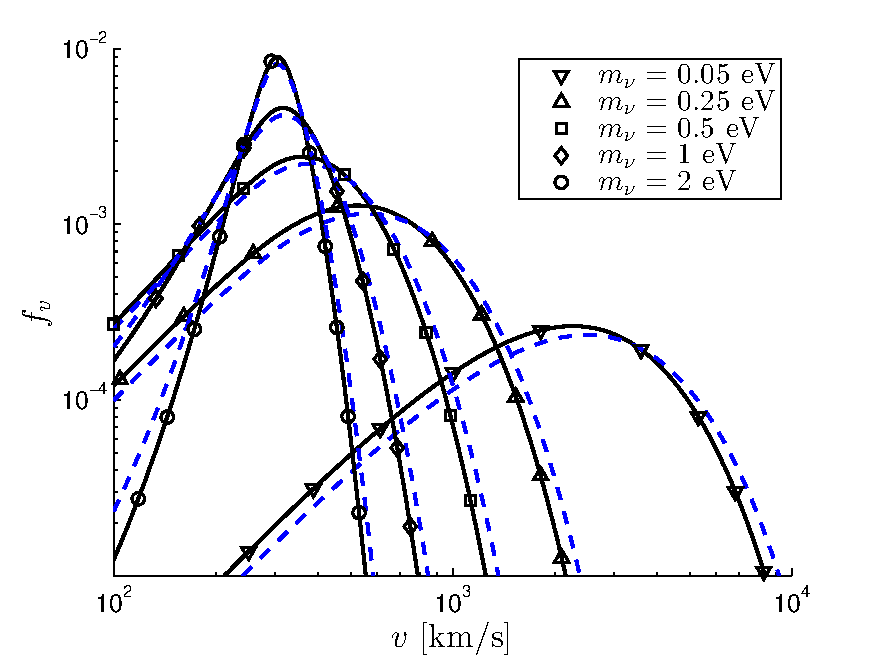
\includegraphics[width=0.9\textwidth]{04-birrell/NeutrinoDistributionToday/Figures/rel_v_dist_300.pdf}}
\caption{Normalized neutrino FDEV velocity distribution in the Earth frame. We show the distribution for $N_\nu^{\mathrm{eff}}=3.046$ (solid lines) and $N_\nu^{\mathrm{eff}}=3.62$ (dashed lines). \cccite{Birrell:2014qna}}
\label{fig:rel_v_dist_300}
 \end{figure}
%%%%%%%%%%%%%%%%%%%%%%%%%%%%%%%%%%%%%%%

A similar procedure produces the normalized FDEV energy distribution $f_E$.  In \req{fvdistrib} we replace $dp/dv\to dp/dE$ where it is understood that 
\begin{equation}
p(E)=\sqrt{E^2-m_\nu^2},\qquad \frac{dp}{dE}=\frac{E}{p}.
\end{equation}
We show $f_E$ in Figure \ref{fig:E_dist_300}  for several values of the neutrino mass, $v_{\text{rel}}=300$ km/s, and $N_\nu^{\mathrm{eff}}=3.046$ (solid lines) and $N_\nu^{\mathrm{eff}}=3.62$ (dashed lines). The width of the FDEV energy distribution is on the micro-eV scale and the kinetic energy $T=E-m_\nu$ is peaked about $T=\frac{1}{2}m_\nu v_{\text{rel}}^2$, implying that the relative velocity between the Earth and the CMB is the dominant factor for $m_\nu>0.1$ eV.

%%%%%%%%%%%%%%%%%%%%%%%%%%%%%%%%%%%%%%%
\begin{figure}
\centerline{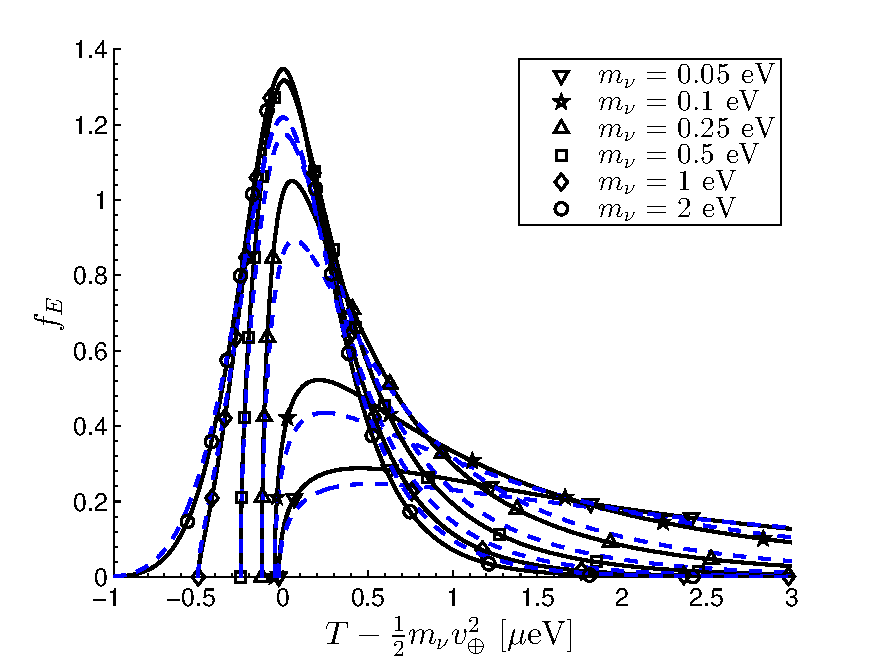
\includegraphics[width=0.9\textwidth]{04-birrell/NeutrinoDistributionToday/Figures/E_dist_300.pdf}}
\caption{Neutrino FDEV energy distribution in the Earth frame. We show the distribution for $N_\nu=3.046$ (solid lines) and $N_\nu=3.62$ (dashed lines). \cccite{Birrell:2014qna}}
\label{fig:E_dist_300}
 \end{figure}
%%%%%%%%%%%%%%%%%%%%%%%%%%%%%%%%%%%%%%%

By multiplying $f_E$ by the neutrino velocity and number density for a single neutrino flavor (without anti-neutrinos) we obtain the particle flux density,
 \begin{equation}
 \frac{dJ}{dE}\equiv\frac{dn}{dAdtdE}\,,
\end{equation} 
shown in Figure \ref{fig:flux_dist}. We show the result for $N_\nu^{\mathrm{eff}}=3.046$ (solid lines) and $N_\nu^{\mathrm{eff}}=3.62$ (dashed lines). The flux is normalized in these cases to a local denisty $56.36$~cm${}^{-3}$ and $60.10$~cm${}^{-3}$ respectively. 

The precise neutrino flux in the Earth frame is significant for efforts to detect relic neutrinos, such as the PTOLEMY experiment~\cite{Betts:2013uya}. The energy dependence of the flux shows a large sensitivity to the mass. However, the maximal fluxes do not vary significantly with $m$. In fact the maximum values are independent of $m$ when $v_{\text{rel}}=0$, as follows from the fact that $v=p/E=dE/dp$.  In the Earth frame, where $0<v_\oplus\ll c$, this translates into only a small variation in the maximal flux.

%%%%%%%%%%%%%%%%%%%%%%%%%%%%%%%%%%%%%%%
\begin{figure}
\centerline{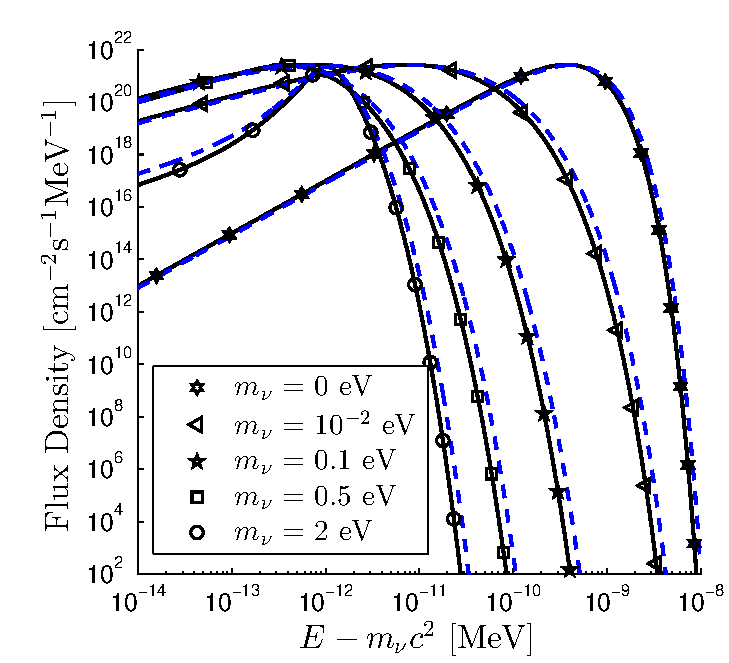
\includegraphics[width=0.9\textwidth]{04-birrell/NeutrinoDistributionToday/Figures/flux_dist.pdf}}
\caption{Neutrino flux density in the Earth frame. We show the result for $N_\nu^{\mathrm{eff}}=3.046$ (solid lines) and $N_\nu^{\mathrm{eff}}=3.62$ (dashed lines) for an observer moving with $v_\oplus=300$\,km/s. \cccite{Birrell:2014qna}}
\label{fig:flux_dist}
 \end{figure}
%%%%%%%%%%%%%%%%%%%%%%%%%%%%%%%%%%%%%%%

Using $\lambda=2\pi/p$ we find  the normalized FDEV de Broglie wavelength distribution
\begin{equation}
%\frac{dn}{d\lambda}
f_\lambda=\frac{ 2\pi g_\nu}{n_\nu\lambda^4}\!\!\int_0^\pi\!\!\! \!\frac{\sin(\phi) d\phi}{\Upsilon^{-1}e^{\sqrt{( E-v_{\text{rel}} p \cos(\phi))^2\gamma^2-m_\nu^2}/T_\nu}\!\!+\!1}\,,
\end{equation}
shown in Figure \ref{fig:deBrogle_300} for $v_{\text{rel}}=300$ km/s and for several values $m_\nu$ comparing  $N_\nu^{\mathrm{eff}}=3.046$ with $N_\nu^{\mathrm{eff}}=3.62$. %  While the FDEV distributions are peaked at the millimeter wavelength scale, to discriminate dependence on neutrino masses it is necessary to consider somewhat larger wavelengths. 

%%%%%%%%%%%%%%%%%%%%%%%%%%%%%%%%%%%%%%%
\begin{figure} 
\begin{minipage}{\textwidth}
\makebox[0.5\linewidth]%
{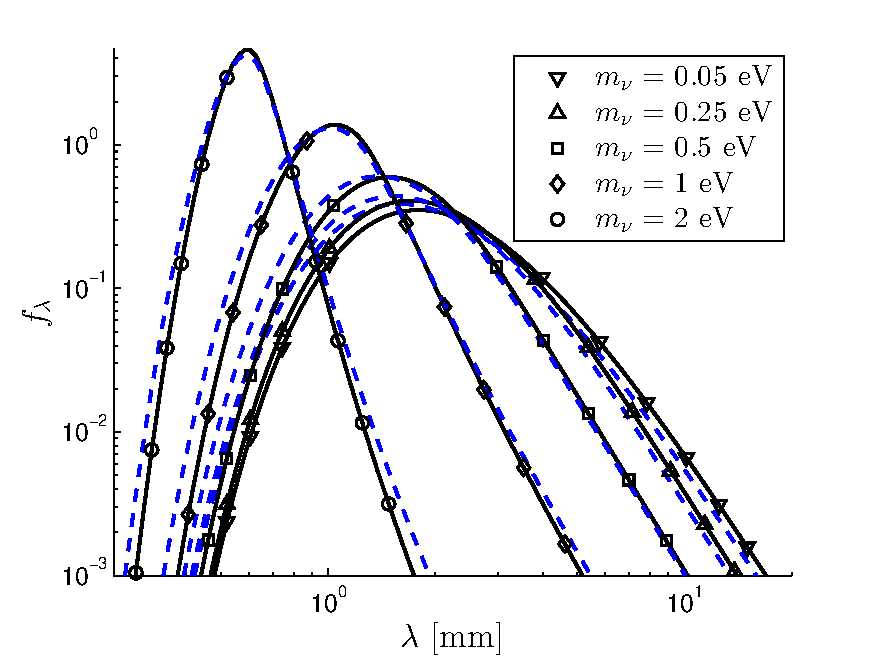
\includegraphics[height=5.4cm]{04-birrell/NeutrinoDistributionToday/Figures/deBrogle_300.pdf}}
\makebox[0.5\linewidth]%
{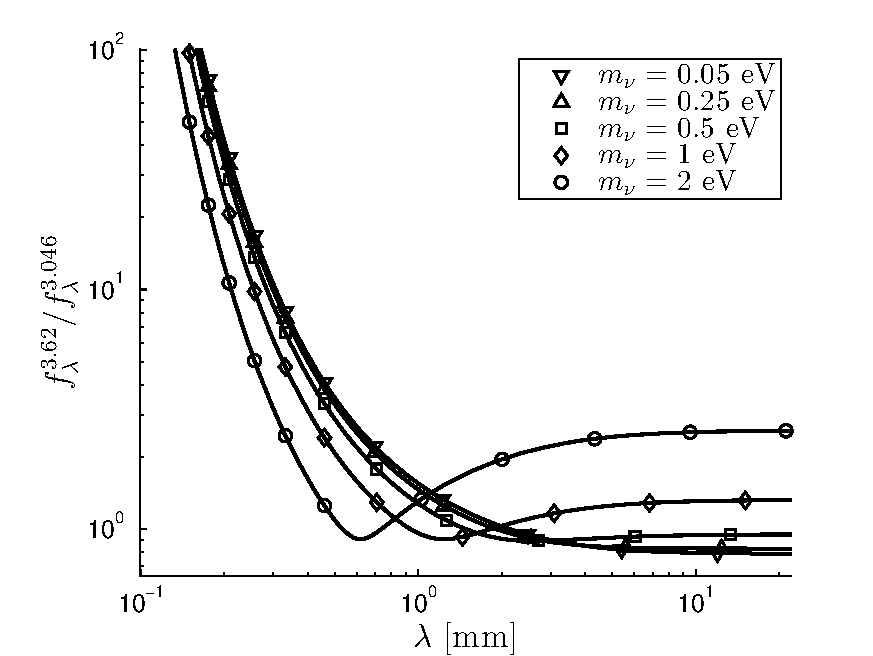
\includegraphics[height=5.4cm]{04-birrell/NeutrinoDistributionToday/Figures/f_ratio.pdf}}
\end{minipage}
\caption{Neutrino  FDEV de Broglie wavelength  distribution in the Earth frame. We show in left panel the distribution for $N_\nu^{\mathrm{eff}}=3.046$ (solid lines) and $N_\nu^{\mathrm{eff}}=3.62$ (dashed lines) and in right panel their ratio. \cccite{Birrell:2014qna}.  }\label{fig:deBrogle_300}
 \end{figure}
%%%%%%%%%%%%%%%%%%%%%%%%%%%%%%%%%%%%%%%%%%%%%%%%%

%%%%%%%%%%%%%%%%%%%%%%%%%%%%%%%
\para{Drag Force}
Given the neutrino distribution, we evaluate the drag force due to the anisotropy of the neutrino distribution in the rest frame of the moving object for $N_\nu^{\mathrm{eff}}=3.046$. The relic neutrinos will undergo potential scattering with the scale of the potential strength being
\begin{equation}\label{V0}
V_0=CG_F\rho_{N_c},\hspace{2mm} \rho_N\equiv N_c/R^3
\end{equation}
where $R$ is the linear size of the detector.  

When the detector size is smaller than the quantum de Broglie wavelength of the neutrino, all scattering centers are added coherently to for the target effective `charge' $N_c$.  $\rho_{N_c}$ is the charge density, and C=O(1) and is depending on material composition of the object. Such considerations are of interest both for scattering from terrestrial detectors, as well as for ultra-dense objects of neutron star matter density, e.g.   strangelet  CUDOS~\cite{Rafelski:2011bby} - recall that such nuclear matter fragments with $R<\lambda$  despite their small size would have a mass rivaling that of large meteors. We find $V_0\simeq 10^{-13}$ eV for normal matter densities, but for nuclear target density a potential well with $V_0\simeq {\cal O}(10 {\rm eV})$.  

We consider relic neutrino potential scattering to obtain the average momentum transfer to the target and hence the drag force. The particle flux per unit volume in momentum space is
\begin{equation}\label{dn_quantum}
\frac{dn}{dtd Ad^3{\bf p}}({\bf p})=\frac{2}{(2\pi)^3}f({\bf p})p/m_\nu\,,\hspace{2mm} p\equiv |{\bf p}|\,,
\end{equation}
where the factor of two comes from combining neutrinos and anti-neutrinos of a given flavor. 

Our use of non-relativistic velocity is justified by  \rf{fig:rel_v_dist_300}.  The recoil change in detector momentum per unit time is  
\begin{align}
\frac{d{\bf p}}{dt}=& \int  {\bf q}A \frac{dn}{dtdAd^3p}({\bf p})d^3p\,,\\
{\bf q}A\equiv &\int ({\bf p}-{\bf p_f})\frac{d\sigma}{ d\Omega}({\bf p_f},{\bf p})d\Omega\,.
\end{align}
Here ${\bf p}$ and ${\bf p}_f$, the incoming and outgoing momenta respectively, have the same magnitude. $qA$ is the momentum transfer times area, averaged over outgoing momenta, and $d\Omega$ is the solid angle for to ${\bf p}_f$.  

For a spherically symmetric potential the differential cross section depends only on the incoming energy and the angle $\phi$ between ${\bf p}$ and ${\bf p_f}$.  Therefore, for each ${\bf p}$ the integral over $d\Omega$ of the components orthogonal to ${\bf p}$ is zero by symmetry.  This implies
\begin{align}
{\bf q}A\equiv &2\pi{\bf p}\int(1-\cos(\phi))\frac{d\sigma}{ d\Omega}(p,\phi)\sin(\phi)d\phi\,.
\end{align}
The only angular dependence in the neutrino distribution is in ${\bf p}\cdot {\bf\hat z}$ and therefore the components of the force orthogonal to ${\bf \hat z}$ integrate to zero, giving
\begin{align}\label{drag}
\frac{d{\bf p}}{dt}=&\frac{{\bf\hat z}}{\pi m_\nu } \int p^4g(p) f(p,\tilde\phi) \cos(\tilde\phi) \sin(\tilde\phi) dpd\tilde\phi\,,\\
g(p)\equiv& \int_0^\pi(1-\cos(\phi))\frac{d\sigma}{ d\Omega}(p,\phi)\sin(\phi)d\phi\,.\label{geq}
\end{align}

For the case of normal density matter, the Born approximation is valid due to the weakness of the potential compared to the neutrino energy seen in Figure \ref{fig:E_dist_300}. To obtain an order of magnitude estimate, we take a Gaussian potential \begin{equation}
V(r)=V_0e^{-r^2/R^2}
\end{equation}
for which the differential cross section in the Born approximation can be analytically evaluated
\begin{align}
&\frac{d\sigma}{ d\Omega}(p,\phi)=\frac{\pi m_\nu^2V_0^2R^6}{4}e^{-q^2R^2/2}\,,\notag\\
&q=|{\bf p}-{\bf p}_f|=2p\sin(\phi/2)\,.
\end{align}

The integral over $\phi$ in \req{geq} can also be done analytically, giving
\begin{align}
g(p)=&\pi m_\nu^2V_0^2R^6\frac{1-(2R^2p^2+1)e^{-2R^2p^2}}{4R^4p^4}\,.
\end{align}
 In the long and short wavelength limit we have 
\begin{align}
\label{long_wave_drag}
&g(p)\simeq\frac{\pi}{2} m_\nu^2V_0^2R^6\,,\quad pR\ll 1\,,\\
&F_L\simeq \frac{m_\nu V_0^2R^6}{2} \int p^4 f(p,\tilde\phi) \cos(\tilde\phi) \sin(\tilde\phi) dpd\tilde\phi\,,\notag\\
\label{short_wave_drag}
&g(p)\simeq\frac{\pi m_\nu^2V_0^2R^2}{4p^4}\,, 
\quad pR\gg 1\,,\\
&F_S\simeq \frac{ m_\nu V_0^2R^2}{4} \int f(p,\tilde\phi) \cos(\tilde\phi) \sin(\tilde\phi) dpd\tilde\phi\notag\,.
\end{align}
 We also note that in the short wavelength limit, our coherent scattering treatment is only applicable to properly prepared structured targets \cite{Liao:2012wb}.

Inserting \req{V0} we see that this force is $O(G_F^2)$, see also \cite{Shvartsman,Smith:1983jj,Gelmini:2004hg}, as compared to the $O(G_F)$ effects debated in  \cite{Opher:1974drq,Lewis:1979mu,Opher2,Cabibbo:1982bb,Langacker:1982ih,Smith:1983jj,Ferreras:1995wf}. In long wavelength limit the size $R$ cancels, in favor of $N_c^2$ which explicitly shows that scattering is on the square of the charges of the target. 

This results in an enhancement of the force by a factor of $N_c$ over the incoherent scattering case, due to $V_0^2$ scaling with $N_c^2$. This effect exactly parallels the proposed detection of supernovae MeV energy scale neutrinos by means of collisions with the entire atomic nucleus~\cite{Divari:2012zz}.  

Fits to the integrals in the above force formulas \req{long_wave_drag} and \req{short_wave_drag} can be obtained in the region $0.005 \text{eV}\leq m_\nu\leq 0.25\text{eV}$, $v_\text{rel}\leq 300$km/s, yielding
\begin{align}\label{F_L}
F_L\!=&8\,10^{-34}{\rm N}\!\left(\!\frac{m_\nu}{0.1 \text{eV}}\!\right)^{\!\!2}\!\! \left(\!\frac{V_0}{1\text{peV}}\!\right)^{\!\!2}\!\!\left(\!\frac{R}{1\text{mm}}\!\right)^{\!\! 6} \!\!\frac{v_{\text{rel}}}{v_\oplus},\\[0.2cm]
F_S=&2\, 10^{-35}{\rm N}\!\left(\!\frac{m_\nu}{0.1\text{eV}}\!\right)^{\!\!2}\! \left(\!\frac{V_0}{1\text{peV}}\!\right)^{\!\!2}\!\!\left(\!\frac{R}{1\text{mm}}\!\right)^{\!\!2}\times\notag \\
&\hspace*{1.5cm}\times\frac{v_{\text{rel}}}{v_\oplus}\!\left(\!1\!-\!0.2\frac{m_\nu}{0.1\text{eV}}\frac{v_{\text{rel}}}{v_\oplus}\right).
\end{align}
We emphasize that they are not valid in the limit as $m_\nu\rightarrow 0$. Considering that the current frontier of precision force measurements at the level of individual ions is on the order of $10^{-24}$N \cite{Biercuk}, the ${\cal O}(G_F^2)$ force on a coherent mm-sized terrestrial detector is negligible, despite the factor of $N_c$ enhancement. 

We now consider scattering from nuclear matter density $\rho_N\simeq 3 \, 10^{8}{\rm kg/mm}^3$ objects where $V_0={\cal O}(10\text{eV})$ is effectively infinite compared to the neutrino energy unless the object velocity relative to the neutrino background is ultra-relativistic.  Therefore we are in the hard `ball' scattering limit. As with the analysis for normal matter density, we will investigate both the long and short wavelength limits. 

In the long wavelength limit, only the S-wave contributes to hard sphere scattering and $d\sigma/d\Omega=R^2$, independent of angle. Using \req{drag} and a similar fit to \req{F_L} gives
\begin{align}\label{FLHard}
F_L=&\frac{2\pi^2R^2}{\pi m_\nu} \int p^4 f(p,\tilde\phi) \cos(\tilde\phi) \sin(\tilde\phi) dpd\tilde\phi\notag\\
\simeq &\, 2\, 10^{-22}{\rm N}\left(\frac{R}{1\text{mm}}\right)^2\frac{v_{\text{rel}}}{v_\oplus}\,.
\end{align}
In particular the force is independent of $m_\nu$.  We also note that at high velocity, \req{FLHard}  underestimates the drag force. The resulting acceleration is
\begin{equation}
a=4\, 10^{-31}\frac{m}{s^2}\frac{v_{\text{rel}} }{v_\oplus}\! \left(\frac{R}{1\text{mm}}\right)^{-1}\!\!\left(\frac{\rho}{\rho_N}\right)^{-1}\,.\!\!
\end{equation}

The Newtonian drag time constant, $v_{\rm rel}/a$, is
\begin{equation}
\tau= 2\,10^{28}\text{yr}\frac{R}{1\text{mm}}\,\frac{\rho}{\rho_N}\,,
\end{equation}
which suggests that the compact object produced early on in stellar evolution remain largely unaltered.

The last case to consider is the short wavelength hard sphere scattering limit.  This limit is classical and so we no longer treat it as quantum mechanical potential scattering, but rather as elastic scattering of point particle neutrinos from a hard sphere of radius $R$.  

For a single scattering event where the component of the momentum normal to the sphere is ${\bf p}^\perp=({\bf p}\cdot \hat {\bf r}) \hat {\bf r}$, the change in particle momentum is  $\Delta {\bf p}=-2{\bf p}^\perp$. The particle flux per unit volume in momentum space at a point ${\bf r}$ on a radius $R$ sphere $S_R^2$ and inward pointing momentum ${\bf p}$ (i.e. ${\bf p}\cdot \hat{\bf  r}<0$) is
\begin{equation}\label{dn_classical}
\frac{dn}{dtd Ad^3{\bf p}}({\bf x},{\bf p})=\frac{2}{(2\pi)^3}f({\bf p})|{\bf v}\cdot \hat{\bf r}|\,,
\end{equation}
where the factor of two comes from combining neutrinos and anti-neutrinos of a given flavor.  

Note that for point particles the flux is proptional to the normal component of the velocity, as opposed to wave scattering where it is proportional to the magnitude of the velocity, seen in \req{dn_quantum}.

Using \req{dn_classical}, the recoil change in momentum per unit time is  
\begin{equation}
\frac{d{\bf p}}{dt}= -\frac{2}{(2\pi)^3}\int_{{\bf p}\cdot \hat{\bf r}<0} \!\!\!\!\!\!\Delta {\bf p}  f({\bf p}) \frac{1}{m_\nu}|{\bf p}\cdot \hat{\bf r}| d^3{\bf p}R^2d\Omega\,.
\end{equation}
The only angular dependence in $f$ is through ${\bf p}\cdot \hat {\bf z}$ so by symmetry, the ${\bf \hat x}$ and ${\bf \hat y}$ components integrate to $0$.  Therefore we have
\begin{equation}
\frac{d{\bf p}}{dt}=-\frac{R^2\hat{\bf z}}{2\pi^3m_\nu}\int_{{\bf p}\cdot \hat{\bf r}<0}\!\!\!   f({\bf p}) ({\bf p}\cdot \hat{\bf r})^2 \hat {\bf r}\cdot\hat{\bf z}\, d^3{\bf p}d\Omega\,.  
\end{equation}

We perform this integration in spherical coordinates for ${\bf r}$ and in the spherical coordinate vector field basis for ${\bf p}=p_r\hat{\bf r} +p_\theta\hat{\bf r}_\theta+p_\phi\hat{\bf r}_\phi,\hspace{2mm} p_r<0$, where we recall
\begin{align}
&\hat{\bf r}=\cos  \theta \sin \phi \, \hat{\bf x}+\sin \theta \sin \phi \hat{\bf y}+\cos  \phi\,\hat{\bf z}\notag\,,\\
&\hat{\bf r}_\theta=-\sin \theta \hat{\bf x}+\cos \theta \hat{\bf y}\,,\\
&\hat{\bf r}_\phi=\cos \theta \cos \phi\,\hat{\bf x}+\sin \theta \cos \phi \,\hat{\bf y}-\sin \phi \, \hat{\bf z}\notag\,.
\end{align}
Therefore the force per unit surface area is
\begin{align}\label{drag_eq}
\frac{1}{A}\frac{d{\bf p}}{dt}=&-\frac{1}{4\pi^3 m_\nu}\int_0^\pi\!\!\int_{p_r<0}\!\!\!\!\!\!\!\! f({\bf p}) p_r^2  d^3{\bf p}\cos \phi \sin \phi  d\phi\hat{\bf z}\,,\notag\\
f({\bf}p)=&\frac{1}{  \Upsilon^{-1}e^{\sqrt{( E-V_\oplus {\bf p}\cdot \hat {\bf z})^2\gamma^2-m_\nu^2}/T_\nu}+1 }\,,\\
          &{\bf p}\cdot\hat{\bf z}=p_r\cos \phi-p_\phi\sin\phi \,.\notag
\end{align}

We obtain an approximation over the range $v_{\text{rel}}\leq v_\oplus ;\ 0.05\text{eV}\leq m_\nu\leq 0.25\text{eV}$ given by
\begin{align}\label{drag_fit}
&F_S =  4\,10^{-23} \text{N}\left(\frac{R}{1{\rm mm}}\right)^2\frac{v_{\text{rel}}}{ v_\oplus}\,.
\end{align}
This is a similar result to the long wavelength hard sphere limit \req{FLHard}, but the fact that it is only applicable to objects larger than the neutrino wavelength means that the acceleration it generates is negligible on the timescale of the Universe.

%%%%%%%%%%%%%%%%%%%%%%%%%%%%%%%%%%
\para{Prospects for Detecting Relic Neutrinos}
In this section we characterized the relic cosmic neutrinos and their velocity, energy, and de Broglie wavelength distributions in a frame of reference moving relative to the neutrino background. We have shown explicitly the mass $m_\nu$ dependence and the dependence on neutrino reheating expressed by $N_\nu^{\mathrm{eff}}$, choosing a range within the experimental constraints. This is a necessary input for the measurement of $N_\nu^{\mathrm{eff}}$ and neutrino mass by future detection efforts.  

Finally, we have discussed in detail the $O(G_F^2)$ mechanical drag force  originating in the dipole anisotropy induced by motion relative to the neutrino background.  Despite enhancement with the total target charge found within the massive neutrino wavelength, the magnitude of the force is found to be well below the reach of current  precision force measurements.

Our results are derived under the assumption that $N_\nu^{\mathrm{eff}}$ is due entirely to SM neutrinos, with no contribution from new particle species. In principle future, relic neutrino detectors, such as PTOLEMY~\cite{Betts:2013uya}, will be able to distinguish between these alternatives since the effect of $N_\nu^{\mathrm{eff}}$ as presented here is to increase neutrino flux~\cite{Birrell:2012gg}, see \req{nnu}. However, to this end one must gain precise control over the enhancement of neutrino galactic relic density due to  gravitational effects~\cite{Ringwald:2004np} as well as the annual modulation~\cite{Safdi:2014rza}. 
%%%%%%%%%%%%%%%%%%%
%%%%%Cheng Tao Leptons, neutrons
\section{Charged leptons in cosmic plasma - CTY}\label{Electron}

Charged leptons played significant roles in the dynamics and evolution of the early Universe. They were kept in equilibrium via electromagnetic and weak interactions.  In this chapter, I examine a dynamical model of the abundance of charged leptons $\mu^\pm$ and $e^\pm$ in the early Universe obtaining their disappearance temperature, the condition when they disappear from the particle inventory. Of particular interest is the dense electron-positron plasma present during the early Universe evolution. I study the damping rate and the magnetization process in this dense $e^\pm$ plasma in the early Universe.


%{Introduction\daggerfootnote{This chapter has been published previously as \citet{Gottbrath1999}.}}
%~~~~~~~~~~~~~~~~~~~~~~~~~~~~~~~~~~~~~~~~~~~~~~~~~

\subsection{Overview of charge leptons in early Universe}
%In this section we will focus on the following:
%\begin{itemize}
%    \item Charged leptons in early universe
%    \item Remarks on tau leptons
%\end{itemize}


%In the early universe, charged leptons are kept equilibrium with the cosmic plasma via electromagnetic and weak interactions which played significant roles in the dynamics and evolution of the Universe.  For example, the present $e^\pm$ in early universe can affect  the neutrino decoupling, photon heating, and big bang nucleosynthesis. Although, the massive lepton $\tau^\pm, \mu^\pm$ decay into light leptons ($\nu$, $l^\pm$) and hadrons in their lifespan. These high-energy leptons ($\nu$, $l^\pm$) originating from the decay of $\tau^\pm, \mu^\pm$ continue played a significant role in shaping the particle energy distribution which can affect the property of cosmic plasma.



The $\tau^\pm$ leptons can undergo various decay processes via the weak interaction in the early Universe, and is the only charged lepton that can decay into hadrons because of its heavy mass ($m_\tau=1776.86$ MeV). The principle decay channels of $\tau^\pm$ are given by
\begin{align}
&\tau^-\rightarrow\nu_\tau+e^-+\bar{\nu}_e,\qquad \tau^-\rightarrow\nu_\tau+\mu^-+\bar{\nu}_\mu,\\
&\tau^-\rightarrow\nu_\tau+\pi^-,\qquad\qquad\,\tau^+\rightarrow\bar{\nu}_\tau+\pi^+,
\end{align}
 where the vacuum lifespan for $\tau^\pm$ is given by ~[\cite{ParticleDataGroup:2022pth}]
\begin{align}
&\tau_{\tau}=(290.3\pm0.5)\times10^{-15}\,\mathrm{sec}.
\end{align}

Moreover, following the decay of $\tau^\pm$ into pions, these pions subsequently decay into a muon and a neutrino through the reaction
\begin{align}
\pi^-\rightarrow\nu_\mu+\mu^-,\qquad\qquad\,\pi^+\rightarrow\bar{\nu}_\mu+\mu^+,
\end{align}
with pion vacuum lifespan $\tau_\pi=2.6033\times10^{-8}$ sec~[\cite{ParticleDataGroup:2022pth}].
In this scenario, $\tau^\pm$ disappears from the Universe via multiparticle decay processes.
These decay processes can contribute as one of the sources for the production of neutrinos and muons in the early Universe.

The $\mu^\pm$ lepton abundance is an important quantity required for the understanding of several fundamental questions regarding properties of the primordial Universe,  particularly in relation to the freeze-out of strangeness flavor in the early Universe. We recall that the strangeness decay often proceeds into muons, energy thresholds permitting, as the charged kaons K$^\pm$ have a 63\% branching into $\mu+\bar \nu_\mu$. Should muons fall out of thermal abundance equilibrium this would directly impact the detailed balance back-reaction processes. Another, indirect influence on strangeness in early Universe arises through the nearly exclusive decay of charged pions into $\mu+\bar \nu_\mu$. Without chemical abundance equilibrium this back reaction stops too impacting pions and thus all other hadronic particles in the Universe. 

On the other hand, we will show that the lightest charged leptons $e^\pm$ can persist via the reaction $\gamma\gamma\to e^-e^+$ until the temperature $T=20$ keV in the early Universe.  After $T=20$ keV, the positron rapidly disappears through annihilation, leaving only residual electrons to maintain the Universe's charge neutrality. The existence of an electron-positron plasma plays a pivotal role in several aspects of the early Universe as follows: 

1. The role of electron-positron plasma has not received the appropriate attention in the days of precision Big-Bang nucleosynthesis studies. The standard BBN model indicates that the synthesis of light elements typically takes place at temperatures around  $86\,\mathrm{keV}>T_{BBN}>50\,\mathrm{keV}$~[\cite{Pitrou:2018cgg}]. Within this temperature range there are millions of electron-positron pairs per charged nucleon, providing an electron-positron-rich plasma environment for nucleosynthesis which leads to modifications in the Coulomb potential due to the screening effect. Furthermore, the electron-positron densities can reach millions of times normal atomic densities. The presence of  these $e\bar e$-pairs before and during BBN has been acknowledged by Wang, Bertulani and Balantekin~[\cite{Wang:2010px}] nearly a decade ago.

2. The Universe today is filled with magnetic fields at various scales and strengths both within galaxies and in deep extra-galactic space. The origin of these magnetic fields is currently unknown. In the early Universe, when temperature $T>20$ keV, we have dense $e^\pm$ plasma. The significant magnetic moments of electrons and positrons also provide opportunities to investigate spin magnetization process.

Understanding the abundances of muons and electrons/positrons provides essential insights into the evolution of the primordial Universe.  In the following we discuss the muon density at persistence temperature in section \ref{section_muon}, and explore the electron/positron plasma properties, including the damped rate and magnetization in section \ref{section_electron}.

%~~~~~~~~~~~~~~~~~~~~~~~~~~~~~~~~~~~~~~~~~~~~~~~~~

\subsection{Muon–antimuon in the early Universe}\label{section_muon}
%In this section we will focus on the following:
%\begin{itemize}
%    \item Vanishing of muon in early Universe
%    \item Muon density at persistence temperature
%\end{itemize}

%\subsection{Vanishing of muon in early Universe}
Our interest in strangeness flavor freeze-out in the early Universe requires the understanding of the abundance of muons in the early Universe. The specific question needing an answer is at which temperature muons remain in abundance (chemical) equilibrium established predominantly by electromagnetic and weak interaction processes, allowing detailed-balance back-reactions to influence strangeness abundance.


In the early Universe in the the cosmic plasma muons of mass $m_\mu=105.66$\,MeV can be produced by the following interaction processes
\begin{align} 
&\gamma+\gamma\longrightarrow\mu^++\mu^-,\qquad & e^++e^-\longrightarrow \mu^++\mu^-\;,\\
&\pi^-\longrightarrow\mu^-+\bar{\nu}_\mu,\qquad & \pi^+\longrightarrow\mu^++\nu_\mu\;.
\end{align}
The back reactions for all above processes are in detailed balance, provided all particles shown on the right hand side (RHS) exist in chemical abundance equilibrium in the Universe. We recall the empty space (no plasma) at rest lifetime of pions $\tau_\pi=2.6033\times10^{-8}$ sec. 

However, all produced muons can also decay via the reactions
\begin{equation}
\mu^-\rightarrow\nu_\mu+e^-+\bar{\nu}_e,\qquad \mu^+\rightarrow\bar{\nu}_\mu+e^++\nu_e\,,
\end{equation} 
with the empty space (no plasma) at rest lifetime $\tau_{\mu}=2.197 \times 10^{-6}\,\mathrm{sec}$. We thus must establish the range of temperature in which production processes exceed in speed the decay process.
 
 The temperature range of our interests is the Universe when $m_\mu\gg T$. In this case the the Boltzmann approximation is appropriate for studying massive particles muons and pions. The thermal decay rate per volume and time  for muons $\mu^\pm$ (and pions $\pi^\pm$) in the Boltzmann limit  are given by~[\cite{PhysRevC.82.035203}]:
\begin{align}
&R_\mu=\frac{g_\mu}{2\pi^2}\left(\frac{T^3}{\tau_\mu}\right)\left(\frac{m_\mu}{T}\right)^2K_1(m_\mu/T)\;,\\
&R_\pi=\frac{g_\pi}{2\pi^2}\left(\frac{T^3}{\tau_\pi}\right)\left(\frac{m_\pi}{T}\right)^2K_1(m_\pi/T)\;, 
\end{align}
where the lifespan of $\mu^\pm$ and $\pi^\pm$ in the vacuum were given above. This rate accounts for both the density of particles in chemical abundance equilibrium and the effect of time dilation present when particles are in thermal motion with respect to observer at rest in the local reference frame. The effects of Fermi blocking or boson stimulated emission have been neglected.

The thermal averaged reaction rate per volume for the reaction $a\overline{a}\rightarrow b\overline{b}$ in Boltzmann approximation is given by [\cite{Letessier:2002ony}]
\begin{align}\label{pairR}
R_{a\overline{a}\rightarrow b\overline{b}}=\frac{g_ag_{\overline{a}}}{1+I}\frac{T}{32\pi^4}\int_{s_{th}}^\infty ds\frac{s(s-4m^2_a)}{\sqrt{s}}\sigma_{a\overline{a}\rightarrow b\overline{b}}~K_1(\sqrt{s}/T),
\end{align}
where $s_{th}$ is the threshold energy for the reaction, $\sigma_{a\overline{a}\rightarrow b\overline{b}}$ is the cross section for the given reaction, and $K_1$ is the modified
Bessel function of integer order ``$1$". We introduce the factor $1/1+I$ to avoid the double counting of indistinguishable pairs of particles; we have $I=1$ for an identical pair and $I=0$ for a distinguishable pair.

The leading order invariant matrix elements for the reactions $e^++e^-\to\mu^++\mu^-$ and $\gamma+\gamma\to\mu^++\mu^-$, are introduced in this work by [\cite{Kuznetsova:2008jt}]
\begin{align}\label{Mee}
|M_{e\bar e\to\mu\bar\mu}|^2=&32\pi^2\alpha^2\frac{(m_\mu^2-t)^2+(m_\mu^2-u)^2+2m_\mu^2s}{s^2},\quad m_\mu\gg m_e\;,\\[0.2cm]
\label{Mgg}
|M_{\gamma\gamma\to\mu\bar\mu}|^2=&32\pi^2\alpha^2\bigg[\left(\frac{m_\mu^2-u}{m_\mu^2-t}+\frac{m_\mu^2-t}{m_\mu^2-u}\right)+4\left(\frac{m_\mu^2}{m_\mu^2-t}+\frac{m_\mu^2}{m^2_\mu-u}\right)\\[0.1cm]  \nonumber
&\hspace{1cm}-4\left(\frac{m_\mu^2}{m^2_\mu-t}+\frac{m^2_\mu}{m^2_\mu-u}\right)^2\bigg]\;,
\end{align}
 where $s, t, u$ are the Mandelstam variables. The cross section required in Eq.\,(\ref{pairR}) can be obtained by integrating the matrix elements Eq.\,(\ref{Mee}) and Eq.\,(\ref{Mgg}) over the Mandelstam variable $t$ ~[\cite{PhysRevC.82.035203}]. We have
\begin{align}
&\sigma_{e\bar e\to\mu\bar\mu} 
=\frac{64\pi\alpha^2}{48\pi}\left(\frac{1+2m^2_\mu/s}{s-4m_e^2}\right)\sqrt{1-\frac{4m^2_\mu}{s}},\\
&\sigma_{\gamma\gamma\to\mu\bar\mu}=\frac{\pi}{2}\left(\frac{\alpha}{m_\mu}\right)^2(1-\beta^2)\left[(3-\beta^4)\ln\frac{1+\beta}{1-\beta}-2\beta(2-\beta^2)\right],\\
&\beta=\sqrt{1-4m^2_\mu/s}
\end{align}
Substituting the cross sections into Eq.\,(\ref{pairR}) we obtain the production rates for $e\bar e\to\mu\bar\mu$ and $\gamma\gamma\to\mu\bar\mu$ respectively.

 
In Fig.~\ref{MuonRatenew_fig} we show the invariant thermal reaction rates per volume and time for rates of relevance, as a function of temperature $T$.
As the temperature decreases in the expanding Universe, the initially dominant production rates ($e\bar e,\gamma\gamma\to\mu\bar\mu$) decrease with decreasing temperature, and eventually cross the $\mu^\pm$ decay rates. 
Muon abundance disappears as soon as any decay rate is faster than the fastest production rate. Specifically after the Universe cools below the temperature $T_\mathrm{disappear}=4.195$ MeV, the dominant reaction is the muon decay. Due to the relatively slow expansion of the Universe, the disappearance of muons is sudden, and the abundance of muons vanishes as soon as a decay rate surpasses the dominant production rate.
 

%~~~~~~~Figure~~~~~~ ~~~~~~~~~~~~~~~~~~~~~~~~~~~~~~~~~~~~~~~~~~~~~~~~~~~~~~~~~~~~~~~~~~~
\begin{figure}[ht]
\begin{center}
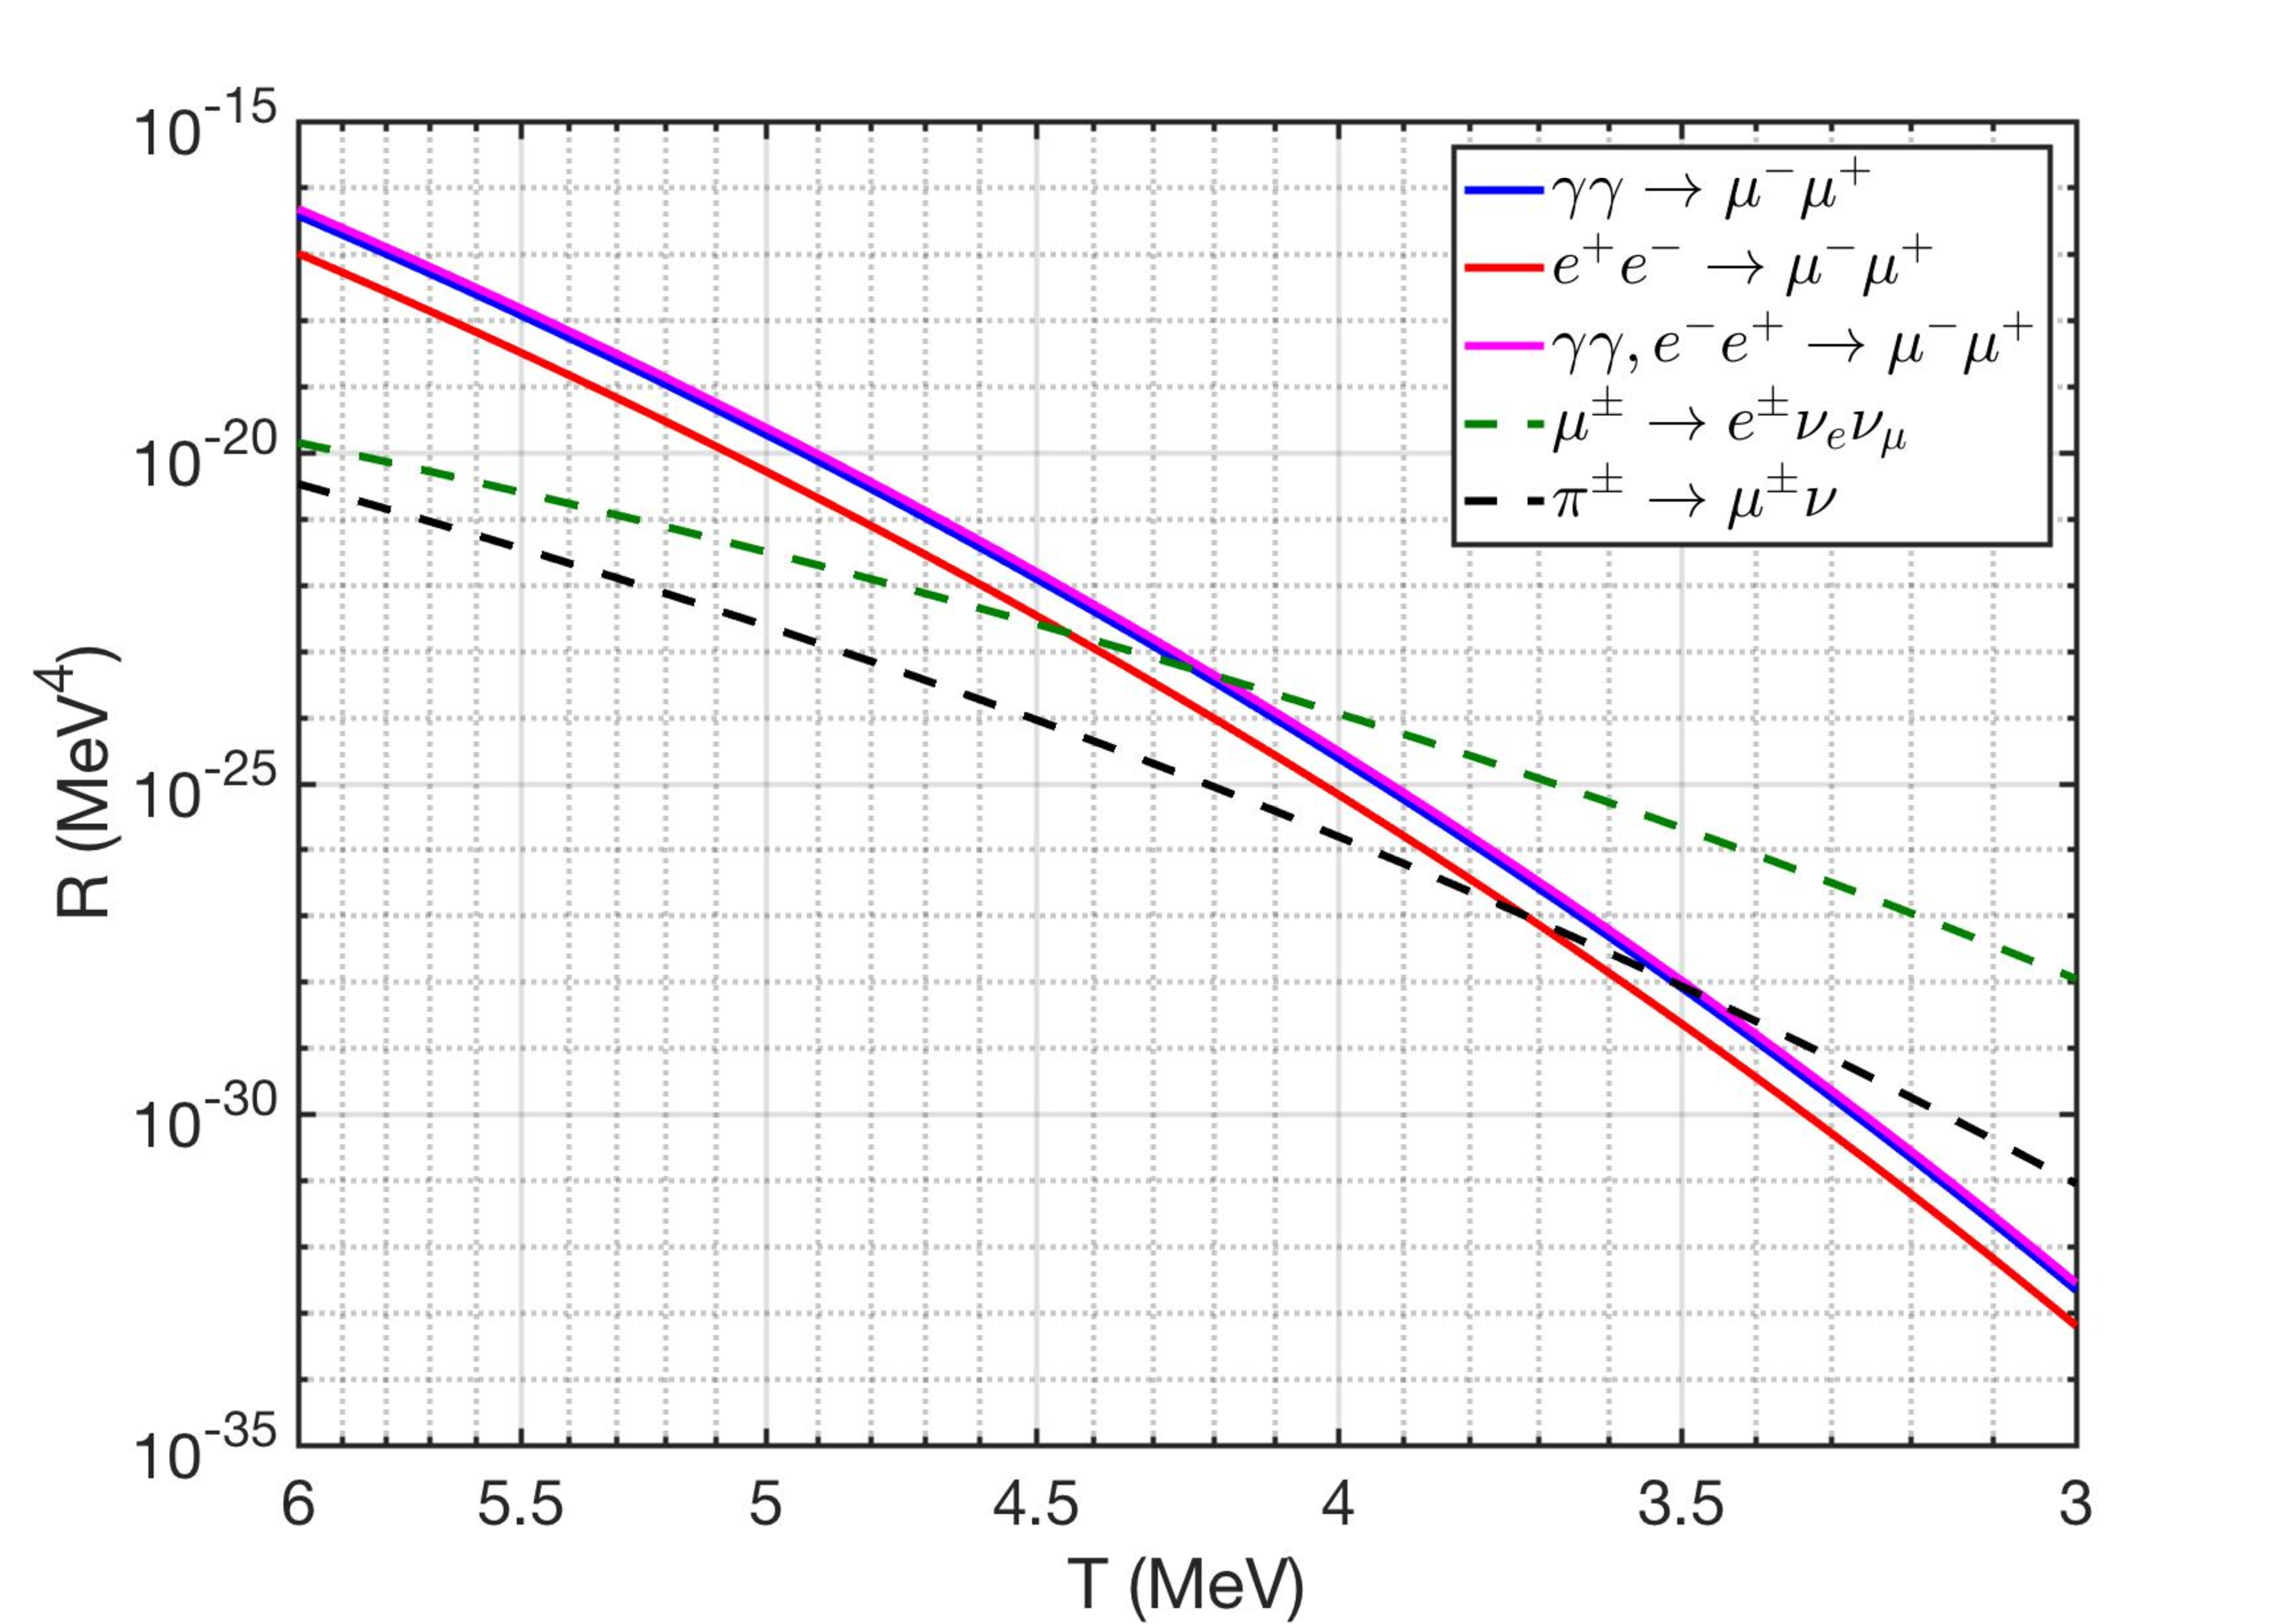
\includegraphics[width=5.0in]{./plots/MuonRate_new2.pdf}
\caption{We plot the thermal reaction rate per volume for different reactions as a function of temperature. We found that dominant reactions for $\mu^\pm$ production are ${\gamma+\gamma\to\mu^++\mu^-}$ and $e^++e^-\to\mu^++\mu^-$, and the total production rate crosses the decay rate of $\mu^\pm$ at temperature $T_{dissapear}\approx 4.195$ MeV.}
\label{MuonRatenew_fig}
\end{center}
\end{figure}
%~~~~~~~~~~~~~~~~~~~~~~~~~~~~~~~~~~~~~~~~~~~~~~~~~~~~~~~~~~~~~~~~~~~~~~~~~~~~~~~~~~~~~~~~~~~~~~~~

On the other hand, considering the number density for nonrelativistic $\mu^\pm$ in the Boltzmann approximation, we have
\begin{align}\label{nmupm}
n_{\mu^\pm}=\frac{g_{\mu^\pm}}{2\pi^2}T^3\left(\frac{m_\mu}{T}\right)^2 K_2(m_\mu/T)=g_{\mu^\pm}\left(\frac{m_\mu T}{2\pi}\right)^{3/2}e^{-{m_\mu}/{T}}\;. 
\end{align}
then the number density between $n_{\mu^\pm}$ and baryon $n_B$ can be written as
\begin{align}
\frac{n_{\mu^\pm}}{n_\mathrm{B}}=\frac{n_{\mu^\pm}}{s}\frac{s}{n_\mathrm{B}}=
\frac{n_{\mu^\pm}}{s}\left(\frac{s}{n_\mathrm{B}}\right)_{\!t_0},
\end{align}
where we used that $s/n_\mathrm{B}$ remains constant and $t_0$ represent present day value. The present value is given by $(n_B/s)_{t_0}\approx8.69\times10^{-11}$ (detail please see Chapter~\ref{Introduction}). The entropy density $s$ can be characterized introducing $g^s_\ast$, the total number of \lq entropic\rq\ degrees of freedom
\begin{align}\label{entrop}
s=\frac{2\pi^2}{45}g^s_\ast T^3\;.
\end{align}
For temperature $10\,\mathrm{MeV} >T>3 $\,MeV, the massless photons, nearly relativistic electron/positrons, and practically massless neutrinos contribute to the degree of freedom $g^s_\ast$.  In this case, the number density between $n_{\mu^\pm}$ and baryon $n_B$ in the temperature interval we consider $10\,\mathrm{MeV} >T>3 $\,MeV is given by
\begin{align}\label{nmuperbF} 
\frac{n_{\mu^\pm}}{n_\mathrm{B}}=\frac{45}{2\pi^2}\frac{g_{\mu^\pm}}{g^s_\ast}\left(\frac{m_\mu}{2\pi T}\right)^{3/2}e^{-{m_\mu}/{T}}\;\left(\frac{s}{n_\mathrm{B}}\right)_{\!t_0}.
\end{align}


%Figure~~~~~~~~~~~~~~~~~~~~~~~~~~~~~~~~~~~~~~~~~~~~~~~~~~~~~~~~~~~~~~~~~~~~~~~~~
\begin{figure}[t]
\begin{center}
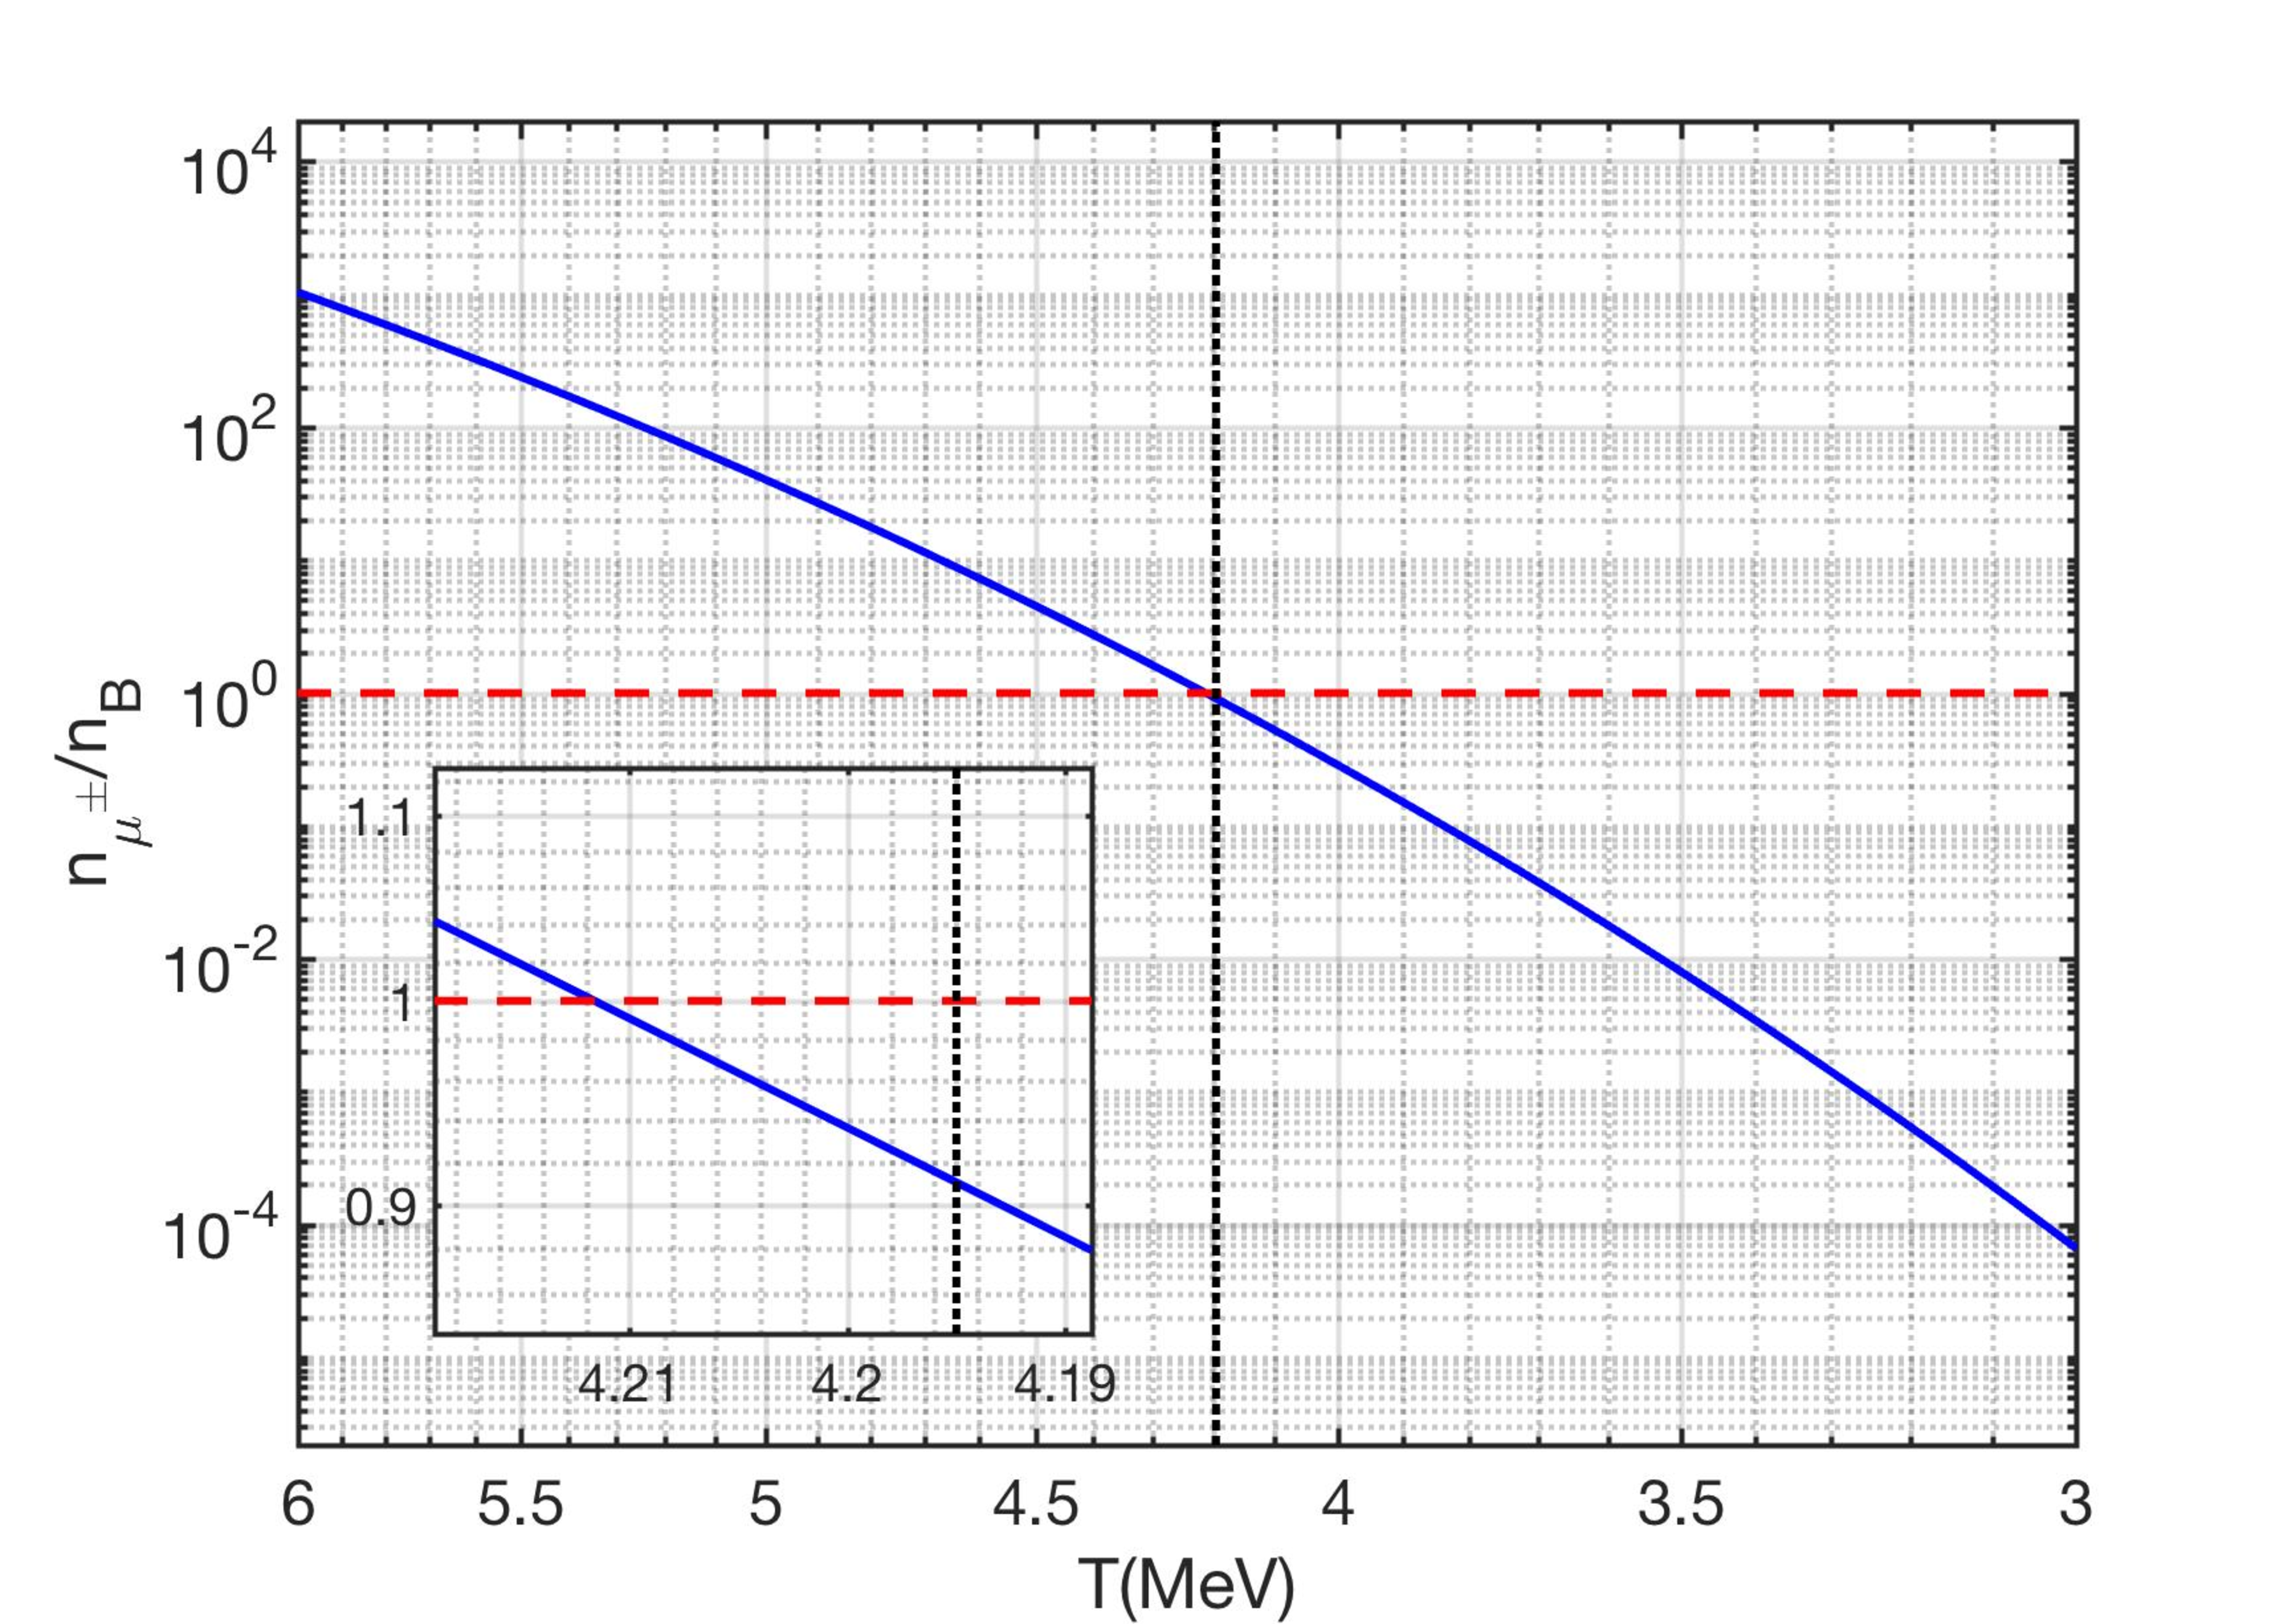
\includegraphics[width=\linewidth]{./plots/DensityRatio_new2.pdf}
\caption{
The density ratio between $\mu^\pm$ and baryons as a function of temperature. The density ratio at muon disappearance temperature is about $n_{\mu^\pm}/n_\mathrm{B}(T_\mathrm{disappear})\approx0.911$, and around the temperature $T\approx4.212$ MeV the density ratio $n_{\mu^\pm}/n_\mathrm{B}\approx1$.}
\label{DensityRatio_fig}
\end{center}
\end{figure}
%~~~~~~~~~~~~~~~~~~~~~~~~~~~~~~~~~~~~~~~~~~~~~~~~~~~~~~~~~~~~~~~~~~~~~~~~~~~~~


In Fig.\,\ref{DensityRatio_fig} we show the muon to baryon density ratio Eq.\,(\ref{nmuperbF}) as a function of $T$. We see that the muon abundance $T=10$\,MeV exceeds that of baryons by a factor 500,000 while at muon disappearance temperature $n_{\mu^\pm}/n_\mathrm{B}(T_\mathrm{disappear})\approx0.911$. The number density $n_{\mu^\pm}$ and $n_\mathrm{B}$  abundances are equal at around the temperature $T_\mathrm{equal}\approx4.212\,\mathrm{MeV} >  T_\mathrm{disappear}$.  This means that the muon abundance may still be able to influence baryon evolution because their number density is comparable to the baryon density.% However, we also find that at the temperature $T_\mathrm{equal}\approx4.212$\,MeV the density ratio is unity $n_{\mu^\pm}/n_\mathrm{B}\approx1$.

The primary insight of this work is that aside of protons, neutrons and other nonrelativistic particles, both positively and negatively charged muons $\mu^\pm$ are present in thermal equilibrium and in non-negligible abundance for $T>T_\mathrm{dissapear}\approx 4.195$\,MeV. This offers a new and tantalizing model building opportunity for anyone interested in baryon-antibaryon separation in the primordial Universe, strangelet formation, and perhaps other exotic primordial structure formation mechanisms.

%%%%%%%%%%%%%%%%%%%%%%%%
% Chapters from Christopher Grayson's dissertation
%%%%%%%%%%%%%%%%%
\section{Plasma physics methods applied to Strong Fields and BBN}\label{part4}
\subsection{Plasma response to electromagnetic fields}
\label{chap:PlasmaSF}

The interaction of electromagnetic fields within relativistic plasmas is of interest in astrophysics, intense laser interactions with matter, and quark-gluon plasma in relativistic heavy-ion collisions\index{heavy-ion!collisions}. Quark-gluon plasma (QGP), a state of matter of deconfined quarks and gluons at extremely high temperatures $T>150$ MeV, is formed in the violent collision of heavy-ions at relativistic speeds. This deconfined state is also of astrophysical interest since it filled the early universe for the first few microseconds after the Big-Bang\index{Big-Bang}. Several methods have been introduced to study the linear response of a collisionless ultrarelativistic QGP following the seminal work by~\cite{Weldon:1982aq} by using semiclassical transport theory based on the Boltzmann equation~\cite{Mrowczynski:1987jr,Mrowczynski:1989np,Blaizot:1993zk,Kelly:1994ig,Kelly:1994dh}. However, applications of this formalism are restricted to dilute plasmas where collisions can be neglected~\cite{Blaizot:2001nr}. 
Previously, the effects of collisions within the plasma were mainly studied to derive transport coefficients, such as the electrical conductivity, of interest to the study of plasma response to long-wavelength perturbations~\cite{Mrowczynski:1988xu,Heiselberg:1993cr,Ahonen:1996nq,Baym:1997gq,Ahonen:1998iz}. In quantum field theory, transport coefficients have also been calculated using effective propagators that re-sum thermal modifications to avoid infrared divergences~\cite{Heiselberg:1994ms,Arnold:2002zm,Arnold:2003zc}. Here, we will study semi-classical transport using the Vlasov-Boltzmann equation\index{Vlasov-Boltzmann equation} with momentum-averaged quantum collisions between particles, a topic discussed in numerous other works, such as \cite{DeGroot:1980dk,Cercignani:2002bk,Hakim:2011bk,Carrington:2003je,Schenke:2006xu}.


The theoretical description of relativistic plasma is based on transport theory, i.e., the relativistic form of Liouville's equation. The one-particle phases space distribution function $f(x,p)$ undergoes Liouville flow,
\begin{align}
    \frac{d f(x,p)}{d\tau} = \{H(x,p), f(x,p)\} = 0\,,
\end{align}
where $p$ is the canonical four-momentum, and $x$ is the canonical position. The collision term $C[f]$ represents elastic/inelastic interactions and gives deviations away from Liouville's theorem
\begin{align}\label{eq:LpC}
    \frac{d f(x,p)}{d\tau} = C[f]\,,
\end{align}
or equivalently, entropy generation. The collision term is necessary to describe systems where the mean free path of plasma constituents is less than or equal to the characteristic length scale of the plasma or when the mean free time $\tau$ is smaller than the characteristic oscillation time of the plasma. This pertains to systems with high density, low temperature, or strongly coupled systems.

The Boltzmann-Einstein equation, see Section \ref{sec:BoltzmannEinstein}, with a realistic collision operator, i.e., modeling scattering among neutrinos and $e^\pm$, was used in Section \ref{ch:param:studies} to  study the cosmological neutrino freeze-out. However, in many cases a detailed treatment of the microscopic collision term \req{eq:collisionMicro} is computationally prohibitive.  In this section our focus is on the interaction of electromagnetic fields within relativistic plasmas and so in place of the microscopic collision term we employ the relaxation-time approximation (RTA) technique, as proposed by~\cite{Anderson:1974nyl}. RTA is a commonly made simplification to the Boltzmann equation, reducing it from an integrodifferential equation to a differential equation. The relativistic form of this collision term takes the form
\begin{equation}\label{eq:lincoll}
C[f] = (p^\mu u_\mu) \kappa [ f_\mathrm{eq}(p) - f(x,p) ] \,,
\end{equation}
where $\kappa=1/\tau$ is the relaxation rate, $f(x,p)$ is the phase space distribution of charged particles in the plasma, $f_\mathrm{eq}(p)$ is their equilibrium distribution, and $u_\mu$ is the 4-velocity of the plasma rest frame.

The RTA collision term assumes the nonequilibrium distribution $f$ returns to the equilibrium distribution in some characteristic time $\tau$, which is evident when writing \req{eq:LpC} in the form
\begin{equation}
    \frac{d f(x,p)}{dt} = \frac{f_\mathrm{eq}(p) - f(x,p) }{\tau}\,.
\end{equation}
The relaxation time $\tau$ can be computed using the schematic relaxation time approximation where an average relaxation time is introduced~\cite{Mrowczynski:1988xu,Satow:2014lia} or by calculating the momentum-dependent relaxation rate $\kappa(p)$ with the input of perturbative matrix elements~\cite{Ahonen:1996nq}. We use the average relaxation time approximation with momentum averaged $\kappa$ to make all calculations analytically tractable.

The well-known disadvantage of the RTA is that it forces all quantities, even conserved ones, to return to their equilibrium value at a rate $\tau$. This can cause the dynamics derived from this collision term to violate current and energy-momentum conservation. The violation of energy conservation is similar to introducing frictional damping into one particle Newtonian dynamics where energy is lost to the environment.

Correcting for current and energy-momentum conservation is possible by adding terms that ensure that conserved quantities are unaffected~\cite{Bhatnagar:1954zz,Greene1973,Rocha:2021zcw,Singha:2023eia}. It is worth noting that this breaking of conservation law does not always affect the physical behavior of the plasma. For instance, the behavior of transverse waves in an infinite homogeneous plasma is unaffected by the addition of current conservation~\cite{Formanek:2021blc}.

In this work, we generalize the BGK modification of the linearized collision term to relativistic plasmas using the Anderson-Witting form Eq.\,(\ref{eq:lincoll}), ensuring current conservation \req{eq:collision} but not energy-momentum conservation. In \cite{Formanek:2021blc} we show that the resulting linear response functions satisfy current conservation and gauge invariance constraints. 

The preceding sections will discuss obtaining exact solutions for the covariant polarization tensor in linear response limit via Fourier transform with the BGK collision term \req{eq:collision}. We will present the plasma's electromagnetic properties by using the polarization tensor to derive the electromagnetic fields.

%%%%%%%%%%%%%%%%%%%%%%%%%%%%%%%%%%%%%%%%%%%%%%%%%%%%%%%%%%%%%%%%%%%%%%%%%%%%%%%%%%%%%%
\para{Covariant kinetic theory}\label{sec:CKT}
A full microscopic picture of plasma kinematics, useful in numerical simulations, is often more involved than what is required to understand changes in the macroscopic quantities of plasmas. A conventional simplification to the microscopic picture is to average over the discrete states to yield a distribution function $f(x,\boldsymbol{p})$, which describes the probability of finding some number of particles $dN$ in a small range of position $d\mathbf{r}^3$ and momentum $d\boldsymbol{p}^3$ or relativistically~\cite{Hakim:2011bk}
\begin{equation}
    \int_{\Sigma}d\Sigma_{\mu}\int  d^4p\frac{p^\mu}{m}f(x,p) = N,
\end{equation}
where $d\Sigma_\mu$ is the surface element on $\Sigma$
\begin{equation}
    d\Sigma_\mu = \frac{1}{3!}\epsilon_{\mu \nu \alpha\beta} dx^\nu \times dx^\alpha\times dx^\beta\,
\end{equation}
% \begin{equation}
%     dN d\tau  = f(x,p)\frac{dx^4 d^4p}{(2\pi)^4}4\pi \delta_+(p^2-m^2).
% \end{equation}
with the covariant integration, measure can be written as
\begin{equation}\label{eq:measure} 
 \frac{d^4p}{(2\pi)^4}4\pi \delta_+(p^2-m^2) = \left.\frac{d^3p}{(2\pi)^3p^0}\right|_{p^0 = \sqrt{|\boldsymbol{p}|^2 + m^2}} \,,
\end{equation}
where $p^0 = p \cdot u$ in the rest frame of the plasma; see Appendix \ref{ch:vol:forms} for a detailed discussion of the relativistic volume element. The one particle distribution function is effectively the phase space density of the system. We will always refer to the 4-momentum as $p = (p_0, \, \boldsymbol{p})$ and the 3-momentum as $\boldsymbol{p}$.

The kinetic equation describing the evolution of this distribution is the Vlasov-Boltzmann equation\index{Vlasov-Boltzmann equation} (VBE). The VBE is often derived in detail from heuristic arguments see \cite{DeGroot:1980dk,Cercignani:2002bk}. Here, we will outline how it relates to Liouville's theorem. A similar derivation of the equilibrium distribution in the presence of electromagnetic fields is found in \cite{Hakim:2011bk}.
We derive the classical one-species Vlasov-Boltzmann equation from the Liouville theorem
\begin{equation}
    \frac{d f(Q,P)}{d\tau} = \{H(Q,P), f(Q,P)\} = 0\,,
\end{equation}
where $P^{\mu}$ and $Q^{\mu}$ are the canonical coordinates. 
This theorem states that the canonical phase space density is conserved or the one particle phase space density $f(Q,P)$ satisfies the above continuity equation.  The Poisson bracket is explicitly written as 
\begin{equation}
    \frac{d f(Q,P)}{d\tau} = \frac{\partial Q^{\mu}}{\partial \tau}\partial_\mu f(Q,P) + \frac{\partial P^{\mu}}{\partial \tau}\frac{\partial f(Q,P)}{\partial P^{\mu}}\,.
\end{equation}
Since we consider these particles in the presence of electromagnetic fields, we use the relativistic EM Hamiltonian in the Bergmann form
\begin{equation}
    H(Q,P) = \sqrt{(P-q A(Q))_\mu(P-q A(Q))^\mu}\,,
\end{equation}
which contracts the kinetic momentum to give the relativistic energy of a particle in an electromagnetic field. The equations of motion are
\begin{align}
    \frac{\partial Q^{\mu}}{\partial \tau} &= \frac{\partial H(Q,P)}{\partial P_{\mu}}= \frac{(P-q A(Q))^{\mu}}{H(Q,P)}\,,\\
   -\frac{\partial P^{\mu}}{\partial \tau} &= \frac{\partial H(Q,P)}{\partial Q^{\mu}}= - \frac{(P-q A(Q))^{\nu}q \partial_\mu A_\nu(Q)}{H(Q,P)}\,.
\end{align}
If a canonical transformation is applied to our coordinates, the Liouville theorem states that the phase space density remains unchanged. 
The transformation we would like to consider is the transition from kinetic to canonical coordinates where $Q^{\mu}\rightarrow x^{\mu}$ and  $P^{\nu} \rightarrow P^{\nu} - q A^{\nu}(x)$. This new momentum is related to the actual velocity of the particle $P^{\nu} - q A^{\nu}(x) = p^{\mu} = m\frac{d x^{\mu}}{d \tau}$.  We then consider the Liouville theorem for the shifted function,  
\begin{equation}
 \frac{d x^{\mu}}{d \tau}\partial_\mu f(x,P-q A(x)) + \frac{d (P-q A(x))^{\mu}}{d \tau}\frac{\partial f(x,P-q A(x))}{\partial (P-q A(x))^{\mu}}\,.
\end{equation}
Then, we use the equations of motion to write
\begin{equation}
    \frac{(P-q A(x))^{\mu}}{H(x,P)} \partial_\mu f(x,P-q A(x)) + q\frac{(P-q A(x))_{\nu}}{H(x,P)} F^{\mu \nu}(x) \frac{\partial f(x,P-q A(x))}{\partial (P-q A(x))^{\mu}}\,.
\end{equation}
Where the electromagnetic tensor is $F^{\mu \nu} = \partial^{\mu} A^{\nu}  - \partial^{\nu}A^{\mu}$. 
Since the canonical momentum is related to the kinetic momentum by $ P^{\mu}  = m\frac{d x^{\mu}}{d \tau} + q A^{\mu}(x)$, we rewrite the Liouville flow in terms of kinetic momentum $p^\mu = m \frac{dx^\mu}{d\tau}$. Applying Liouville's theorem allows us to set the whole expression to zero to recover the collisionless Vlasov-Boltzmann equation
\begin{equation}
    p^{\mu} \partial_\mu f(x, p) + q  p_{\nu} F^{\mu \nu}(x) \frac{\partial f(x, p )}{\partial  p^{\mu} }=0
\end{equation}
where $ p^{\mu} = m\frac{d x^{\mu}}{d \tau}$. The collision term is then added to allow for deviations from constant phase space density flow
\begin{equation}\label{eq:VBE}
\boxed{(p_k \cdot \partial) f_k(x,p_k) + q_k F^{\mu\nu} p^k_\nu \frac{\partial f_k(x,p_k)}{\partial p_k^\mu} =\sum_l \, (p_k\cdot u)C_{kl}(x,p_k)}\,,
\end{equation}
where there are $k$ equations for each particle species and a $l$ sum over all possible collisions with particle $k$. Usually, we drop the subscript $k$ on momentum if there is no ambiguity. The first term describes the flow or diffusion of particles in the medium, the second term generates an electromagnetic force on particles, and the collision term is on the right-hand side. Generally, each plasma constituent will have a Boltzmann equation and collisions between each species. The collision term represents the detailed microscopic scattering between the plasma constituents. The collision term for the reaction $k+l\rightarrow i+j$ is defined as
\begin{equation}\label{eq:collisionMicro}
    C_{kl}(x,p_k) = \frac{1}{2}\sum^N_{i=1}\sum^N_{j=1}\int \frac{d^3p_l}{(2 \pi)^3p_l^0}\frac{d^3p_i}{(2 \pi)^3p_i^0}\frac{d^3p_j}{(2 \pi)^3p_j^0}\left[f_if_j -f_k f_l
    \right]W_{kl|ij}\,,
\end{equation}
where 
$k,l = 1,2,...,N$ and $W_{ij|kl}$ is the transition rate for the respective collision.
It is important to note that in this framework for a plasma forced by external fields, the collision term is the only way a particle species can impact the dynamics of the phase space distribution of another species.

\para{The BGK collision term}
As discussed previously, the integral in \req{eq:collisionMicro} vastly complicates solving the Vlasov-Boltzmann equation\index{Vlasov-Boltzmann equation}. Instead, we will use a simplified collision term that returns the distribution $f(x,p)$ to equilibrium at some characteristic rate $\kappa = 1/\tau$, reducing \req{eq:VBE} from an integro-differential equation to a differential equation. The relaxation rate or damping rate $\kappa$ is the sum of all possible collisions~\cite{Das:2021bkz}
\begin{equation}
    \kappa_k(p) = \sum^N_{i=1}\sum^N_{j=1}\sum^N_{l=1} \frac{1}{2}\int\frac{d^3p_l}{(2 \pi)^3p_l^0}\frac{d^3p_i}{(2 \pi)^3p_i^0}\frac{d^3p_j}{(2 \pi)^3p_j^0}f_l^{\text{eq}}W_{kl|ij}\,
\end{equation}
In \cite{Formanek:2021blc} we utilize the simplified collision term proposed by Ref.~\cite{Bhatnagar:1954zz} (BGK), which is amended to conserve the current 
\begin{equation}\label{eq:collision}
    \boxed{C(x,p) =\kappa\left(f_{\text{eq}}(p)\frac{n(x)}{{n_{\text{eq}}}} - f(x,p)\right)}\,,
\end{equation}
The nonequilibrium and equilibrium densities are defined covariantly as
\begin{align}
\label{eq:ndef1}n(x) &\equiv 2 \int \frac{d^3p}{(2\pi)^3p^0}(p \cdot u)f(x,p)\,,\\
\label{eq:ndef2}n_\mathrm{eq} &\equiv 2\int \frac{d^3p}{(2\pi)^3p^0}(p \cdot u) f_\mathrm{eq}(p)\,.
\end{align}
The factor of two accounts for the spin degrees of freedom. This correction is also proposed in \cite{Rocha:2021zcw} where they treat the collision term as an operator adding counterterms to ensure that when acting on conserved quantities like energy, momentum, and particle number, the modified collision operator yields zero, thereby respecting the fundamental conservation laws. We can see that \req{eq:collision} explicitly conserves the 4-current~\cite{Formanek:2021blc}
\begin{equation}\label{eq:jmudef}
j_{\mathrm{ind}}^\mu (x)= 2q \int \frac{d^3p}{(2\pi)^3p^0}p^\mu f(x,p)\,,
\end{equation}
by applying $\partial_\mu$ on this expression and substituting back from the Boltzmann equation \req{eq:boltzmanncov}
\begin{equation}
\partial_\mu j^\mu = 2q \int \frac{d^3p}{(2\pi)^3p^0} \left\{-q F^{\mu\nu}p_\nu \frac{\partial f(x,p)}{\partial p^\mu}\right. 
\left. + (p \cdot u)\kappa \left[f_\mathrm{eq}(p) \frac{n(x)}{n_\mathrm{eq}}-f(x,p) \right] \right\}\,.
\end{equation} 
The first term should naturally vanish because the collisionless Vlasov equation preserves 4-current. This can be seen upon integration by parts and use of the antisymmetry of $F^{\mu\nu}$. On the other hand, the collision term vanishes by design - see definitions (\ref{eq:ndef1},\ref{eq:ndef2}). This is in contrast to the Anderson-witting collision term, which does not conserve current \req{eq:lincoll}.

\subsection{Linear response: electron-positron plasma}
The transport properties of electron-positron plasma are governed by three Vlasov-Boltzmann equations \cite{Grayson:2023flr}
\begin{align}\label{eq:VBEf}
(p \cdot \partial) f_\pm(x,p) + &q F^{\mu\nu} p_\nu \frac{\partial f_\pm(x,p)}{\partial p^\mu} = C_\pm(x,p)\,,\\
\label{eq:VBEg}(p \cdot \partial) f_\gamma(x,p) &= C_\gamma(x,p)\,.
\end{align}
The subscripts $-$, $+$, and $\gamma$ indicate the transport equation for electrons, positrons, and photons. These form a system of differential equations for each distribution function $f_i(x,p)$. We suppress the 4-momentum subscript for each species $f_i(x,p) = f_i(x,p_i)$ to simplify notation. 

Since photons cannot couple directly to the electromagnetic field, they do not contribute to the dynamics of the electromagnetic field at first-order polarization response as indicated in Eq.\,(\ref{eq:VBEg}). This is not true for a QCD plasma where gluons could couple directly to an external gluon field.

To find the effect of electrons and positrons on the electromagnetic fields, we use the transport equations \req{eq:VBEf} to find the induced current in the plasma
\begin{equation}
j_{\mathrm{ind}}^\mu(x) = 2\int \frac{d^3 p}{(2 \pi)^3 p^0}p^\mu \left[f_+(x,p)-f_-(x,p)\right]\,,
\end{equation}
found via Fourier transformation and related to the induced current in the linear response equation
\begin{equation}
    \widetilde{j}_{\mathrm{ind}}^{\mu}(k) = {\Pi^{\mu}}_{\nu}(k) \widetilde{A}^{\nu}(k)\,,
\end{equation}
to identify the polarization tensor $\Pi^{\mu}_{\nu}$. To begin, we solve the Vlasov-Boltzmann equation with the BGK collision term
\begin{equation}\label{eq:boltzmanncov}
(p \cdot \partial) f_\pm(x,p) + q F^{\mu\nu} p_\nu \frac{\partial f_\pm(x,p)}{\partial p^\mu} = (p \cdot u)\kappa_\pm\left[f^\mathrm{eq}_\pm(p)\frac{n_\pm(x)}{n^\mathrm{eq}_\pm} - f_\pm(x,p)\right]\,.
\end{equation}
Since the solutions for these equations will differ only by the sign of charge, we need only solve one to understand dynamics. The $\pm$, which indicates electrons or positrons, may be dropped when unnecessary in the equations below.

We assume for the equilibrium distribution the covariant Fermi-Dirac distribution function~\cite{DeGroot:1980dk,Hakim:1967prd}:
\begin{equation}\label{eq:fb}
f^\mathrm{eq}_\pm(x,p) \equiv \frac{1}{e^{([p^{\mu} +q A^\mu (x) ] u_\mu\pm \mu_q)/T} + 1}\,,
\end{equation}
where $p^\mu+q A^\mu (x)$ is the canonical momentum in the presence of an electromagnetic 4-potential, $u^\mu$ is the global 4-velocity of the medium, $T$ denotes the temperature in the medium rest frame, and $\mu_q$ is the chemical potential related to charge. 

The linear response approximation assumes the distribution function can be written as a sum of the equilibrium distribution $f_\mathrm{eq}(x,p)$ plus a small perturbation away from the equilibrium $\delta f(x,p)$
\begin{equation}\label{eq:perturbation}
f(x,p) = f_\mathrm{eq}(x,p) + \delta f(x,p)\,.
\end{equation}
Here the small perturbation $\delta f(x,p)$ is induced by an external electromagnetic field. We expand \req{eq:boltzmanncov} in equilibrium and perturbation terms \cite{melrose2008quantum}
\begin{multline}
    (p \cdot \partial)\left(f_\mathrm{eq}(x,p)+ \delta f(x,p)\right) +  q \left(F_{\mathrm{eq}}^{\mu\nu} +\delta F^{\mu\nu}\right)p_\nu \frac{\partial (f_\mathrm{eq}(x,p)+\delta f(x,p))}{\partial p^\mu} \\ = \kappa (p\cdot u)\left(f_\mathrm{eq} (p)\frac{\delta n(x)}{{n_\mathrm{eq}(x)}} - \delta f(x,p)\right)\,.
\end{multline}
Since the equilibrium expressions are a solution to the collisionless Boltzmann equation, all the equilibrium terms combined are zero. The collision term is constructed to be zero at equilibrium. We will neglect the Lorentz force due to the induced field on the perturbation since it is second order in the perturbation
\begin{equation}
    (p \cdot \partial) \delta f(x,p)+ q \delta F^{\mu\nu}p_\nu \frac{\partial f(x,p)}{\partial p^\mu} = \kappa (p\cdot u)\left(f_{\text{eq}} (x,p)\frac{\delta n(x)}{{n_{\text{eq}}(x)}} - \delta f(x,p)\right)\,.
\end{equation}
where the quantity $\delta n(x)$ is defined following the definitions(\ref{eq:ndef1},\ref{eq:ndef2}) as
\begin{equation}
\delta n (x) \equiv 2 \int \frac{d^3p}{(2\pi)^3p^0} (p \cdot u)\delta f(x,p)\,.
\end{equation}
At this point, we will take the weak field limit of the equilibrium distribution, which assumes the change in energy of a particle due to the electromagnetic field is small in comparison to the thermal energy
\begin{equation}
    \frac{ qA(x)\cdot u}{T}\ll 1\,.
\end{equation}
In this case, the equilibrium distribution becomes the usual
\begin{equation}\label{eq:equilibriumFD}
f^\mathrm{eq}_\pm(x,p) \equiv \frac{1}{e^{(p^{\mu}  u_\mu\pm \mu_q)/T} + 1}\,.
\end{equation}
An explicit solution of the Vlasov-Boltzmann\index{Vlasov-Boltzmann equation}  equation can be obtained more easily in momentum space after a Fourier transformation.  We define the Fourier transform $\widetilde{g}(k^\mu)$ of a general function $g(x^\mu)$ of space-time coordinates as 

\begin{equation}\label{eq:ftdef}
g(x) = \int \frac{d^4k}{(2\pi)^4} \, e^{-i k \cdot x} \, \widetilde{g}(k)\,.
\end{equation} 
The Fourier transformation replaces partial derivatives $\partial_\mu$ with the 4-momentum $k_\mu$:
\begin{equation}
\partial_\mu \rightarrow - i k_\mu \,.
\end{equation}
The 4-vector $k^\mu = (\omega,\mathbf{k})$ represents the momentum and energy in the electromagnetic field. In contrast, $p^{\mu}  = (E,\boldsymbol{p})$ represents the momentum and energy of plasma constituents.

Using these definitions, the Fourier-transformed Boltzmann equation reads \cite{Formanek:2021blc}
\begin{equation}\label{eq:boltzfourier}
-i (p \cdot k) \widetilde{\delta f}(k,p) + q\widetilde{F}^{\mu\nu}p_\nu \frac{\partial f_\mathrm{eq}(p)}{\partial p^\mu} 
= (p \cdot u)\kappa \left[\frac{f_\mathrm{eq}(p)}{n_\mathrm{eq}}\widetilde{\delta n}(k) - \widetilde{\delta f}(k,p) \right]\,.
\end{equation}
In the following, we simplify the notation of derivatives of the equilibrium function with respect to momentum as
\begin{equation}
\frac{\partial f_\mathrm{eq}(p)}{\partial p^\mu} = \frac{d f_\mathrm{eq}(p)}{d (p \cdot u)} u_\mu \equiv f'_\mathrm{eq}(p) u_\mu \,.
\end{equation}
We solve \req{eq:boltzfourier} for the perturbation $\widetilde{\delta f}(k,p)$, which describes fluctuations away from equilibrium due to the electromagnetic field
\begin{equation}\label{eq:deltaftilde}
\widetilde{\delta f}(k,p) = \frac{i}{p \cdot k + i (p \cdot u) \kappa}\bigg[-q (u \cdot \widetilde{F} \cdot p)f'_\mathrm{eq}(p) 
\left.+ (p \cdot u) \kappa \frac{f_\mathrm{eq}(p)}{n_\mathrm{eq}}\widetilde{\delta n}(k)\right]\,.
\end{equation}
This can be readily integrated to obtain an equation for $\widetilde{\delta n}(k)$
\begin{equation}
\widetilde{\delta n}(k) = R(k) - Q(k)\widetilde{\delta n}(k)\,,
\end{equation}
where the integrals are defined as
\begin{align}\label{eq:R}
R(k)  \equiv -2i \int \frac{d^3p}{(2\pi)^3p^0}(p \cdot u) \frac{q(u \cdot \widetilde{F} \cdot p)f'_\mathrm{eq}}{p \cdot k + i (p \cdot u)\kappa}\,,\\
\label{eq:Q}Q(k) \equiv -2i \frac{\kappa}{n_\mathrm{eq}}\int \frac{d^3p}{(2\pi)^3p^0}(p \cdot u)^2 \frac{f_\mathrm{eq}(p)}{p\cdot k + i(p \cdot u)\kappa}\,.
\end{align}
The solution for $\widetilde{\delta n}(k)$ in terms of the external fields is simply 
\begin{equation}
\widetilde{\delta n}(k) = \frac{R(k)}{1+Q(k)}\,.
\end{equation}
We can substitute this result back into (\ref{eq:deltaftilde}) to obtain an explicit expression for $\widetilde{\delta f}(k,p)$ found in \cite{Formanek:2021blc}
\begin{equation}\label{eq:deltafsolution}
	\widetilde{\delta f}(k,p) = \frac{i}{p \cdot k + i (p \cdot u) \kappa}\bigg[-q (u \cdot \widetilde{F} \cdot p)f'_\mathrm{eq}(p) 
	\left.+ (p \cdot u) \kappa \frac{f_\mathrm{eq}(p)}{n_\mathrm{eq}} \frac{R(k)}{1+Q(k)}\right]\,.
\end{equation}
The right-hand side contains only known quantities. In the next section, we will use \req{eq:deltafsolution} to calculate the induced current in the plasma. Adding additional conservation laws requires further integrals to solve the Vlasov-Boltzmann equation involving higher moments of the fluctuation $\delta f$ as discussed in \cite{Rocha:2021zcw,Singha:2023eia}.

%=====================================================================
\para{Induced current}
The induced charge current is the sum of the antiparticle distribution $\widetilde{f}_-$ and the particle distribution $\widetilde{f}_+$
\begin{equation}\label{eq:perturbation1}
\tilde{j}_{\mathrm{ind}}^\mu(k) = 2\int \frac{d^3 p}{(2 \pi)^3 p^0}p^\mu 
\sum_{i = \, +, \, -} q_i \tilde{f}_{i}(k,p)\,,
\end{equation}
with the factor of two accounting for spin. Sometimes, this is referred to as the first moment of $\delta f$.
After expanding in linear response \req{eq:perturbation}, and specifying $q_\pm = \pm e$ the induced current is a function of the perturbation
\begin{align}\label{eq:perturbation2}
\tilde{j}_{\mathrm{ind}}^\mu(k) = 2\int \frac{d^3 p}{(2 \pi)^3 p^0}p^\mu \Big( e \left[\tilde{f}^{\mathrm{eq}}_+(k,p)-\tilde{f}^{\mathrm{eq}}_-(k,p)\right]\notag\\
+ e\left[\delta\tilde{f}_+(k,p)-\delta\tilde{f}_-(k,p)\right]
\Big)
\notag\\
=4 e\int \frac{d^3 p}{(2 \pi)^3 p^0}p^\mu \delta\tilde{f}(k,p)
\,.
\end{align}
The equilibrium currents cancel in the weak field limit for zero chemical potential\index{chemical potential}, and the perturbations add since they differ by the charge $\delta f_\pm=\pm e \delta f' $. For finite chemical potential $\mu_q$, the equilibrium terms can be combined with hyperbolic trig-identities
\begin{equation}
\begin{split}
\tilde{j}_{\mathrm{ind}}^\mu(k) 
=2 e\int \frac{d^3 p}{(2 \pi)^3 p^0}p^\mu \Big(&-\frac{\sinh{(\mu_q)}}{\cosh{(p \cdot u)}+\cosh{(\mu_q)}} \\&+  \left[\delta\tilde{f}_+(k,p)-\delta\tilde{f}_-(k,p)\right]
 \Big)
\,.
\end{split}
\end{equation}
For now, we will focus on the case of zero chemical potential, $\mu_q=0$, where the first term vanishes.
We can express the induced current in terms of defined integrals \cite{Formanek:2021blc} resulting from inserting \req{eq:deltafsolution} into the induced current
\begin{equation}\label{eq:jmu}
\widetilde{j}_{\mathrm{ind}}^\mu(k) = R^\mu(k) - \frac{R(k)}{1+Q(k)} Q^\mu(k)
\end{equation}
where the integrals $R^\mu(k)$ and $Q^\mu(k)$ are defined analogously to (\ref{eq:R},\ref{eq:Q}) as
\begin{align}
\label{eq:Rmu}R^\mu(k)  \equiv -4q^2i \int \frac{d^3p}{(2\pi)^3p^0} p^\mu \frac{(u \cdot \widetilde{F} \cdot p)f'_\mathrm{eq}}{p \cdot k + i (p \cdot u)\kappa}\,,\\
\label{eq:Qmu}Q^\mu(k) \equiv -4qi \frac{\kappa}{n_\mathrm{eq}}\int \frac{d^3p}{(2\pi)^3p^0}(p\cdot u) p^\mu \frac{f_\mathrm{eq}(p)}{p\cdot k + i(p \cdot u)\kappa}\,.
\end{align} 
Note that we absorbed the factor $4e$ from the current (\ref{eq:perturbation2}) into the definition of these integrals. The $R^{\mu}$ term is what one would find from the collisionless case $\kappa \rightarrow 0^+$. The induced current for the normal RTA collision term, which does not conserve current, is obtained by setting $\delta n \rightarrow n_{eq}$ or equivalently
\begin{equation}\label{eq:jRTA}
\widetilde{j}_{\mathrm{AW}}^\mu(k) = R^\mu(k) - Q^\mu(k)
\end{equation}

\para{Covariant polarization tensor}
To find the polarization tensor, we compare our result (\ref{eq:jmu}) to the covariant formulation of Ohm's law~\cite{Starke:2014tfa} which both describe the induced current in the momentum space
\begin{equation}\label{eq:ohm}
\widetilde{j}^\mu(k) = \Pi^\mu_\nu(k) \widetilde{A}^\nu(k)\,.
\end{equation}
To perform this comparison and extract the polarization tensor we must rewrite the Fourier transform of the electromagnetic tensor in terms of the 4-vector potential in momentum space $\widetilde{A}^\mu(k)$
\begin{equation}\label{eq:ftfmunu}
\widetilde{F}^{\mu\nu}(k) = -i k^\mu \widetilde{A}^\nu(k) + i k^\nu \widetilde{A}^\mu(k)\,.
\end{equation}
We then substitute this into the definition of $R^\mu(k)$ (\ref{eq:Rmu}) and isolate $\widetilde{A}^\mu$ as so it is in the form of \req{eq:ohm} to obtain \cite{Formanek:2021blc}
\begin{equation}
R^\mu(k) = - 4q^2 \int \frac{d^3p}{(2\pi)^3p^0} f'_\mathrm{eq}(p)
\times \frac{(u\cdot k)p^\mu p_\nu - (k \cdot p)p^\mu u_\nu}{p\cdot k + i (p \cdot u) \kappa} \widetilde{A}^\nu(k)\,,
\end{equation}
from which we see that the contribution of $R^\mu$ to the polarization tensor is
\begin{equation}\label{eq:Rmunu}
R^\mu_\nu(k) \equiv - 4q^2 \int \frac{d^3p}{(2\pi)^3p^0} f'_\mathrm{eq}(p)
\times\frac{(u\cdot k)p^\mu p_\nu - (k \cdot p)p^\mu u_\nu}{p\cdot k + i (p \cdot u) \kappa}.
\end{equation}
The contribution of the second term is hidden in the $R(k)$ scalar. In terms of the 4-vector potential in the momentum space $\widetilde{A}^\nu$ we have
\begin{equation}
R(k) = - 2q \int \frac{d^3p}{(2\pi)^3p^0}(p \cdot u)f'_\mathrm{eq}(p)
\times\frac{(u\cdot k)p_\nu - (k \cdot p)u_\nu}{p\cdot k + i (p \cdot u) \kappa}\widetilde{A}^\nu(k)\,.
\end{equation}
We can identify in this expression a 4-vector $H_\nu(k)$ defined as
\begin{equation}\label{eq:Hnu}
H_\nu(k) \equiv - 2q \int \frac{d^3p}{(2\pi)^3p^0}(p \cdot u)f'_\mathrm{eq}(p)
\times\frac{(u\cdot k)p_\nu - (k \cdot p)u_\nu}{p\cdot k + i (p \cdot u) \kappa}
\end{equation}
so that the polarization tensor is given by
\begin{equation}\label{eq:pimunu}
\boxed{\Pi^\mu_\nu(k) = R^\mu_\nu(k) - \frac{Q^\mu(k) H_\nu(k)}{1+Q(k)},}
\end{equation}
where the covariant quantities $R^\mu_\nu$, $Q^\mu$, $H_\nu$, and $Q$ are given by the integrals (\ref{eq:Rmunu}, \ref{eq:Qmu}, \ref{eq:Hnu}, \ref{eq:Q}) respectively. 
This is the final covariant form of the current conserving covariant polarization tensor for an infinite homogeneous plasma. The bulk of the work in applying \req{eq:pimunu} to a specific scenario is choosing an equilibrium distribution and evaluating the integrals. Explicit expressions for the components of this tensor in the rest frame of the plasma are found in the ultrarelativistic limit \req{eq:polfuncsUltra} and in the nonrelativistic limit \req{eq:polfuncs} in \cite{Formanek:2021blc}.
This polarization tensor is also derived in \cite{Carrington:2003je} and \cite{Schenke:2006xu}. The correction to the polarization tensor found by using the collision term with current conservation \req{eq:collision} is given by the second term in \req{eq:pimunu}. The current conserving correction modifies the longitudinal polarization properties of the tensor related to charge fluctuations but not the transverse properties related to electromagnetic waves. The Anderson-Witting form of the polarization tensor found using the collision term \req{eq:lincoll} is equivalent to $R^\mu_\nu$ and the polarization tensor for a collisionless plasma is $R^\mu_\nu$ with $\kappa \rightarrow 0^+$.

\subsection{Self-consistent electromagnetic fields in a medium}\label{sec:Maxwell}
To find the electromagnetic field in a plasma, we solve Maxwell's equations self-consistently in an infinite homogeneous and stationary polarizable medium. In this medium, Maxwell's equations take on the usual form \cite{melrose2008quantum}
\begin{equation}
\partial^{[\mu}F^{\nu \rho]}(x) =0, \quad \partial_{\mu}F^{\mu \nu}(x) = \mu_0 J^{\nu}(x)\,,
\end{equation}
Using the Fourier transform defined as in equation \req{eq:ftdef} we replace partial derivatives $\partial_\mu$ with the 4-momentum $-i k_\mu$. Then Maxwell's equations in Fourier space are
\begin{equation}
-i k^{[\mu}\widetilde{F}^{\nu \rho]}(k) =0, \quad -i k_{\mu}\widetilde{F}^{\mu \nu}(k) = \mu_0 \widetilde{J}^{\nu}(k)\,,
\end{equation}
$k=(\omega, \boldsymbol{k})$ is the 4-wavevector of the electromagnetic field. The properties of the medium are introduced by writing the 4-current $\widetilde{J}^{\mu}$ in terms of its induced and external parts
\begin{equation}
 \widetilde{J}^{\mu}(k) = \widetilde{j}_{\mathrm{ext}}^{\mu}(k)+ \widetilde{j}_{\mathrm{ind}}^{\mu}(k)\,.
\end{equation}
The induced current $\widetilde{j}_{\mathrm{ind}}^{\mu}$, to leading order, is given by the polarization tensor through \req{eq:ohm}. Though the induced current is linear with respect to the self-consistent field $\widetilde{A}^{\nu}$, the field itself is intrinsically nonlinear regarding plasma response as we shall see when solving for the self-consistent fields \reqs{eq:phi}{eq:aperp}. Nonlinear response comes from higher-order terms involving nested convolution integrals of the polarization tensor and the self-consistent potential and is required when the polarization current is on the order of the external current.

Solving Maxwell's equations in the Lorentz gauge $k \cdot \widetilde{A}=0$, one finds the usual expression
\begin{equation}\label{eq:Amu}
\begin{split}
\widetilde{A}^{\mu}(k)&= -\frac{\mu_0}{k^2}\left(\widetilde{j}_{\mathrm{ext}}^{\mu}(k)+ \widetilde{j}_{\mathrm{ind}}^{\mu}(k)\right)\\
&= -\frac{\mu_0}{k^2}\left(\widetilde{j}_{\mathrm{ext}}^{\mu}(k)+  \Pi^\mu_\nu(k) \widetilde{A}^\nu(k)\right)\,,
\end{split}
\end{equation}
$\mu_0$ denotes the magnetic permittivity of the vacuum, and we have used \req{eq:ohm} to express the induced current. 

\para{Projection of plasma polarization tensor} We proceed by algebraically solving for the self-consistent potential. To do this, we first note that in a homogeneous medium, the response depends only on two independent scalar polarization functions $\Pi_\parallel$ and $\Pi_\perp$ describing polarization in the parallel and transverse directions relative to the wave-vector $\boldsymbol{k}$ \cite{Weldon:1982aq}. The polarization tensor may be written in terms of these polarization functions as
\begin{equation}\label{eq:poltensgen}
 \Pi^{\mu \nu}(k,u) = \Pi_\parallel(k) L^{\mu \nu}(k,u) + \Pi_\perp(k) S^{\mu \nu}(k,u)\,,
\end{equation}
where $k^\mu$ is the 4-momentum of the field and $u^\mu$ is the 4-velocity of the medium. The polarization tensor represents the electromagnetic response of the medium to the electromagnetic field. $\Pi_\parallel$ usually describes charge fluctuations and $\Pi_\perp$ describes the properties of electromagnetic waves. For optically active or chiral mediums there is also a rotational portion of the polarization tensor $\Pi_R$. Since we neglect spin, our derivation of the polarization tensor is not sensitive to $\Pi_R$. Conventions for the longitudinal and transverse projection tensors, $L^{\mu \nu}$ and  $S^{\mu \nu}$, may be found in \cite{melrose2008quantum}. These tensors are reproduced here for convenience
\begin{equation}
     L^{\mu \nu} \equiv \frac{k^2}{(k\cdot u)^2-k^2}\bigg[ \frac{ k^{\mu}u^{\nu}}{(k\cdot u)}+ \frac{ k^{\nu}u^{\mu}}{(k\cdot u)} -\frac{k^2u^{\mu}u^{\nu}}{(k\cdot u)^2}  -\frac{k^{\mu}k^{\nu}}{k^2} \bigg]\,,
\end{equation}
\begin{equation}
     S^{\mu \nu} \equiv g^{\mu \nu} +\frac{1}{(k\cdot u)^2-k^2}\bigg[ k^{\mu}k^{\nu} 
     -(k\cdot u)( k^{\mu}u^{\nu}+k^{\nu}u^{\mu})+k^2u^{\mu}u^{\nu}\bigg]\,.
\end{equation}
These projections are equivalent to ones defined in \cite{Weldon:1982aq} up to an overall normalization. To simplify the calculation, the wave-vector $\boldsymbol{k}$ is chosen, without loss of generality, to point along the third spatial direction ($\mu=3$):
 \begin{equation}\label{eq:poltenmat}
    \Pi^{\mu}_{\nu}(\omega,\boldsymbol{k}) = \left[
    \begin{array}{cccc}
-\frac{|\mathbf{k}|^2}{\omega^2}\Pi_{\parallel}& 0 & 0 & \frac{|\mathbf{k}|}{\omega}\Pi_{\parallel} \\
 0 & \Pi_{\perp} & 0 & 0 \\
 0 & 0 & \Pi_{\perp} & 0 \\
 -\frac{|\mathbf{k}|}{\omega}\Pi_{\parallel} & 0 & 0 & \Pi_{\parallel} \\ 
\end{array}
\right]\,.
\end{equation}
Utilizing this decomposition, we can immediately see that the transverse polarization function will be related to the $\Pi^1_1 = \Pi^2_2 = \Pi_\perp$ component of the polarization tensor defined in \req{eq:pimunu}. Analogously, the longitudinal portion of the polarization tensor is given by calculating the $\Pi^3_3 = \Pi_\parallel$ component. The spatial component of the potential $\widetilde{\boldsymbol{A}}$  in these coordinates can be expressed as
\begin{equation}
\widetilde{\boldsymbol{A}} = \widetilde{A}_\parallel \hat{\boldsymbol{k}} + \widetilde{\boldsymbol{A}}_\perp\,,
\end{equation}
which implies
\begin{equation}
 \widetilde{A}_{\parallel} = \frac{\boldsymbol{k} \cdot  \widetilde{\boldsymbol{A}}}{|\boldsymbol{k}|}, \quad   \widetilde{\boldsymbol{A}}_{\perp} = \widetilde{\boldsymbol{A}} -  \widetilde{A}_{\parallel}\hat{\boldsymbol{k}}\,,
\end{equation}
\begin{figure}[ht]
    \centering
    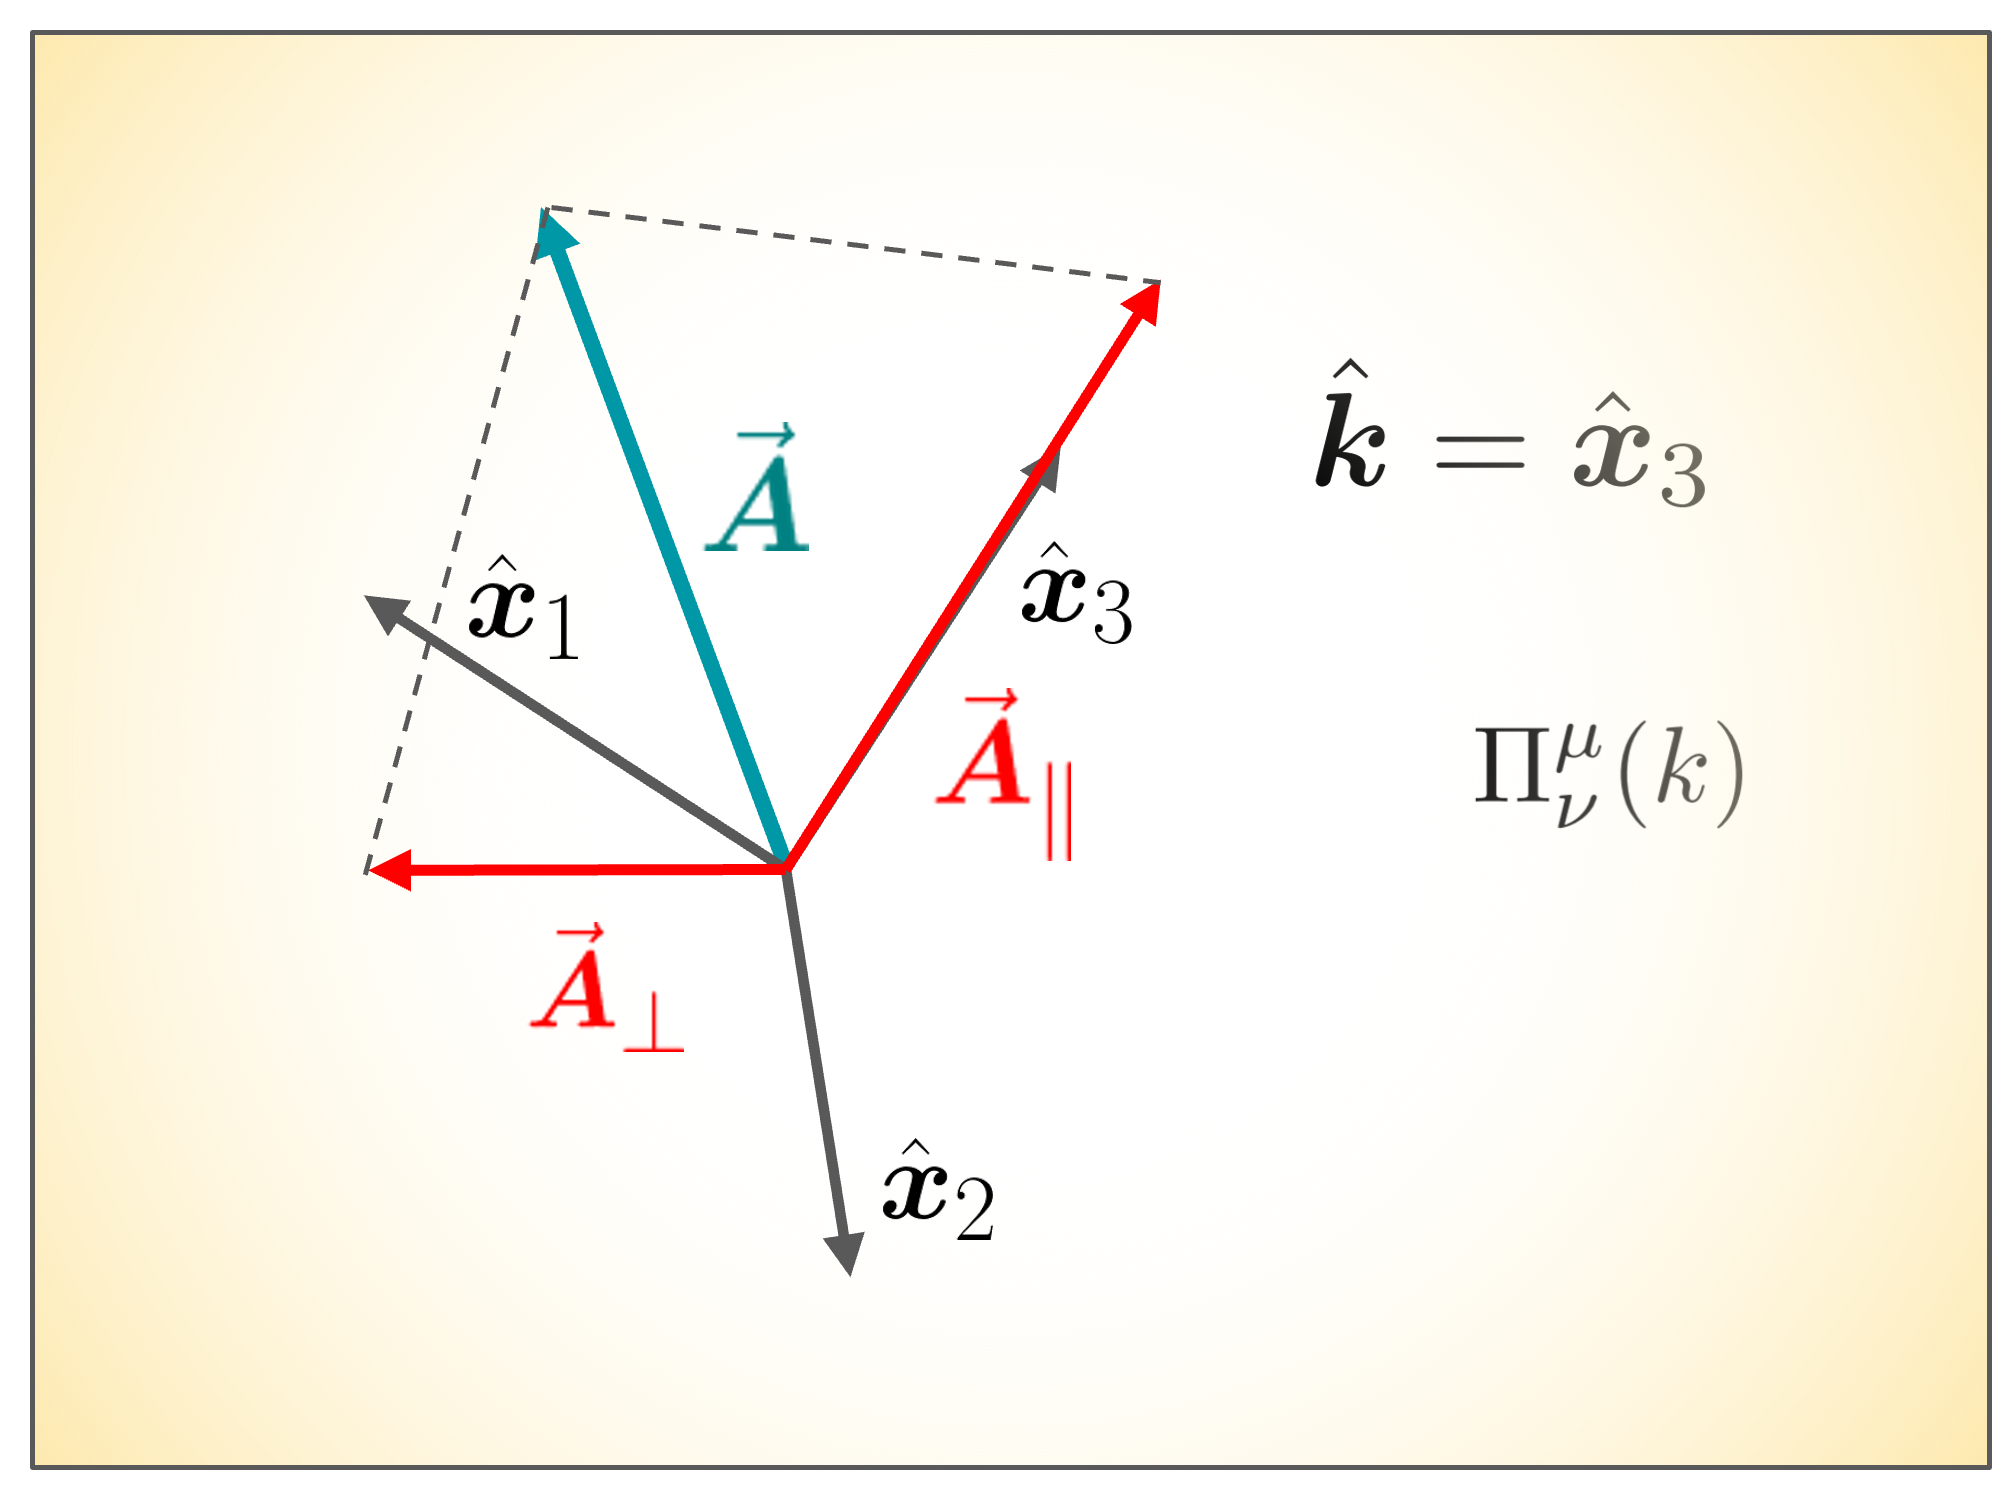
\includegraphics[width=0.55\linewidth]{plots/chap01intro/Screenshot 2024-03-14 124133.png}
    \caption{Vector potential is projected onto $\boldsymbol{\hat{k}} = \boldsymbol{\hat{x_3}} =\boldsymbol{\hat{z}}$. \radapt{Grayson:2024okq}.}
    \label{fig:project}
\end{figure}
with analogous definitions for the current, $\widetilde{j}_{\parallel}$ and $\widetilde{j}_{\perp}$. Note that the Lorentz gauge condition $\partial_\mu A^\mu = 0$ implies
\begin{equation}\label{eq:apar}
\widetilde{A}_\parallel = \frac{\omega}{ |\boldsymbol{k}|}\widetilde{\phi}\, ,
\end{equation} 
with $\phi=A^0$. The induced charge is calculated using the projected polarization tensor \req{eq:poltenmat}:
\begin{equation}
    \widetilde{\rho}_\text{ind}(\omega,\boldsymbol{k})  = \Pi^0_\nu \widetilde{A}^\nu = -\frac{|\boldsymbol{k}|^2}{\omega^2} \Pi_{\parallel}\widetilde{\phi} +  \frac{|\boldsymbol{k}|}{\omega}\Pi_{\parallel} \widetilde{A}_{\parallel}\,.
\end{equation}
For the Lorentz gauge condition \req{eq:apar}, one finds
\begin{equation}\label{eq:indch}
    \widetilde{\rho}_\text{ind}(\omega,\boldsymbol{k})  = \Pi_{\parallel}\widetilde{\phi} \left(1 -\frac{|\boldsymbol{k}|^2}{\omega^2}\right)\,.
\end{equation}
The longitudinal current is,
\begin{equation}\label{eq:indjpar}
\widetilde{j}_{\parallel\text{ind}}(\omega,\boldsymbol{k})  =  \Pi^z_\nu \widetilde{A}^\nu  = \Pi_{\parallel}  \frac{\omega}{|\boldsymbol{k}|}\widetilde{\phi}\left(1-\frac{|\boldsymbol{k}|^2}{\omega^2} \right)\,,
\end{equation}
as expected from current conservation $\partial^\mu j_\mu(x) =0$.
The induced transverse current is
\begin{equation}\label{eq:indjperp}
   \boldsymbol{j}_{\perp\text{ind}}(\omega,\boldsymbol{k})  =  \Pi_{\perp} \widetilde{A}_\perp\,.
\end{equation}
Solving for the potential on both sides of \req{eq:Amu} with the help of \reqs{eq:indch}{eq:indjperp} gives the self-consistent solutions \cite{Grayson:2022asf}
\begin{align}\label{eq:phi}
&\widetilde{\phi}(\omega,\boldsymbol{k}) = \frac{\widetilde{\rho}_\text{ext}(\omega,\boldsymbol{k})}{\varepsilon_0(\boldsymbol{k}^2-\omega^2) \left(\Pi_{\parallel}/( \omega^2\varepsilon_0)+1\right) }\,, \\\label{eq:aperp}
&\widetilde{\boldsymbol{A}}_\perp(\omega,\boldsymbol{k}) = \frac{\mu_0 \widetilde{\boldsymbol{j}}_{\perp \text{ext}}(\omega,\boldsymbol{k})}{\boldsymbol{k}^2 - \omega^2 - \mu_0 \Pi_{\perp}}\,.
\end{align}
The gauge condition \req{eq:apar} gives the self-consistent potential $\widetilde{A}_\parallel$. These self-consistent potentials determine the electric and magnetic fields via the usual relations
\begin{equation}\label{eq:ftfields}
\widetilde{\boldsymbol{B}}(\omega,\boldsymbol{k}) = i\boldsymbol{k} \times \widetilde{\boldsymbol{A}}_\perp\,, \quad \widetilde{\boldsymbol{E}}(\omega,\boldsymbol{k}) = -i \boldsymbol{k} \widetilde{\phi} + i \omega \widetilde{\boldsymbol{A}}\,.
\end{equation}
To obtain the electromagnetic fields in position space, one must Fourier transform \reqs{eq:phi}{eq:aperp}. If done analytically, this usually requires finding the poles in the denominator of these expressions, which equates to finding the poles of the thermal photon propagator. These poles represent propagating modes in the plasma. Modes will often be located at complex values in the $\omega, \mathbf{k}$ plane, leading to finite lifetimes and spatial dispersion. 

\para{Small back-reaction limit}
Here, we briefly mention an alternative to the self-consistent fields, which comes from assuming that the back reaction of the plasma due to the external fields is small compared to the external field. In this case, one can use the external field in the linear response equation instead of the total field
\begin{equation}\label{eq:pert}
    \widetilde{j}_{\mathrm{ind}}^{\mu}(k) = {\Pi^{\mu}}_{\nu}(k) \widetilde{A}_\text{ext}^{\nu}(k)\,.
\end{equation}
Inserting this into \req{eq:Amu} successively to find a series expansion yields the same expression as expanding \reqs{eq:phi}{eq:aperp} in the polarization functions
\begin{align}\label{eq:phipert}
&\widetilde{\phi}(\omega,\boldsymbol{k}) = \sum_{n=0}^\infty\frac{\widetilde{\rho}_\text{ext}(\omega,\boldsymbol{k})}{\varepsilon_0(\boldsymbol{k}^2-\omega^2)}\left(-\frac{\Pi_{\parallel}}{ \omega^2\varepsilon_0}\right)^n\,, \\\label{eq:aperppert}
&\widetilde{\boldsymbol{A}}_\perp(\omega,\boldsymbol{k}) = \sum_{n=0}^\infty\frac{\mu_0 \widetilde{\boldsymbol{j}}_{\perp \text{ext}}(\omega,\boldsymbol{k})}{(\boldsymbol{k}^2 - \omega^2)^{n+1}}(\mu_0 \Pi_{\perp})^{n}\,.
\end{align}
The first term $n=0$ is the vacuum field, and higher-order terms describe the back reaction of the induced current on the external field. Notably, the series expansion of \req{eq:aperp} does not accurately represent the late-time magnetic field in QGP during heavy-ion collisions\index{heavy-ion!collisions}. This is because the infinite series of \reqs{eq:phi}{eq:aperp} must be performed to capture the pole structure of the field. 

Electromagnetic fields in a polarizable medium are often described using the electric displacement field $\mathbf{D}$, the magnetic fields $\mathbf{H}$, the polarization $\mathbf{P}$, and the magnetization $\mathbf{M}$. This formulation is only useful when the field or the medium's response is static or time-dependent. When introducing spatial and temporal dispersion, these definitions are no longer unique \cite{melrose2008quantum}. For instance, if the magnetization depends on space and time $\mathbf{M}(t,x)$ the time dependence of the magnetic field generated will lead to electric fields through Faraday's Law leading to ambiguity since the displacement field no longer depends on just polarization field $\mathbf{P}$.


\subsection{General properties of EM fields in a plasma}
In the case of an infinite homogeneous plasma, its properties are completely described by two independent polarization functions $\Pi_\parallel(k)$ and $\Pi_\perp(k)$. In the framework presented here, the properties of these scalar functions are imparted on the electromagnetic fields via the poles in the Fourier transform of the propagators in \reqs{eq:phi}{eq:aperp}. After contour integration, one effectively gets a sum of different electromagnetic fields at each pole, the amplitude of which depends on the residue of the pole and a spacetime dependence, leading to growth attenuation or propagation depending on the pole's location. An example of this process in done in \cite{Grayson:2022asf}, where we Fourier transform the magnetic field in the center of heavy-ion collisions. 

\para{Dispersion relation}
We can find the poles of the propagator or, equivalently the zeros of the dispersion relation by inverting Maxwell's equations
\begin{equation}
    -ik_{\mu}\widetilde{F}^{\mu \nu} = \mu_0( \widetilde{j}_{\mathrm{ind}}^{\nu}+\widetilde{j}_{\mathrm{ext}}^{\nu})\,.
\end{equation}
Including the induced current on the left-hand side of the equation and writing the expression in terms of $A^{\mu}$ one finds,
\begin{equation}
    (k^2g^{\mu \nu} - k^{\mu} k^{\nu} + \mu_0\Pi^{\mu \nu})\widetilde{A}_{\nu} = - \mu_0\widetilde{j}_{\mathrm{ext}}^{\nu} \,.
\end{equation}
The propagator $D^\mu_\nu(k)$ is obtained by inverting the previous equation
\begin{equation}
    \widetilde{A}_{\nu}(k) = -D^{\mu}_{\nu}(k) \,\widetilde{j}_{\mathrm{ext}}^{\nu}(k) \,.
\end{equation}
The poles of $D^\mu_\nu(k)$ are given by the dispersion equation~\cite{melrose2008quantum}:
\begin{equation}\label{eq:disp}
 \frac{1}{(k\cdot u)^2}\left[(k\cdot u)^2+ \mu_0\Pi_\parallel(k)\right]\left[k^2 + \mu_0 \Pi_\perp(k)\right]^2=0 \,.
\end{equation}
The transverse mode has duplicate solutions as it describes modes in a plane perpendicular to $\boldsymbol{k}$.

The dispersion \req{eq:disp} can be solved for numerous choices of variables describing the modes, such as frequency, phase velocity, or wavevector. We chose to solve for the modes of the plasma in terms of frequency $\omega_m (\mathbf{k})$, which can be thought of as a quasi-particle $m$ with energy $\omega$ and momentum $\mathbf{k}$ analogous to the usual momentum energy relation 
\begin{equation}
    E^2 = \boldsymbol{p}^2 +m^2\, ,
\end{equation}
with $c=1$. This is not always the best choice for simplifying the solutions of \req{eq:disp}, but these modes are often the easiest to interpret. A study of the modes for the general polarization tensor is not the most informative process unless one is looking for general behavior, which can be found in most plasma physics textbooks. Usually, in looking at these modes $\omega_m(\mathbf{k})$, one must first assume the external field's shape or some flow distribution in the plasma by specifying the equilibrium momentum distribution to yield interesting effects in the modes such as plasma instabilities.

When the plasma is perturbed in time in a way that doesn't depend on space, such as for a plane wave, one can take $k \to 0$ for both the transverse and longitudinal roots of the dispersion relation, which reduces the frequency of plasma oscillations \cite{Formanek:2021blc,Grayson:2022asf}
\begin{equation}\label{plasmafreq}
    \omega_{\pm} = -\frac{i\kappa}{2} \pm \sqrt{\omega_p^2 - \frac{\kappa}{4}^2}\,,
\end{equation}
the plasma frequency $\omega_p$ is explicitly given in the ultrarelativistic and nonrelativistic limits, respectively, by \cite{Formanek:2021blc}:
\begin{equation}
\omega_p^2 = \frac{1}{3} m_D^2 \quad (\mathrm{UR})\,, \qquad \omega_p^2 = m_L^2 \quad (\mathrm{NR}) \,,
\end{equation}
with
\begin{equation}
    m_D^2 = \frac{e^2 T}{3}\,.
\end{equation}
The Debye screening mass $m_D$ describes the strength of polarization in the plasma. The plasma frequency $\omega_p$ is the characteristic response frequency of the plasma. For an external field, which is an oscillatory wave of the form $E=E_0e^{-i\omega t}$, one would find that the response is weakly-damped or over-damped depending on the size of $\kappa$ according to \req{eq:plasmafreq}. Waves are weakly damped for $\kappa \ll \omega_p$, and since the square root is imaginary for $\kappa > 2\omega_p$, waves become over-damped. These general statements are subject to the spacetime dependence of the external perturbation. For instance, if a particle moves through the plasma at a constant velocity, the field will not experience much damping if the velocity is much less than the speed of sound in the plasma.

In the static limit $\omega \rightarrow 0$ the zeros in the longitudinal dispersion relation take on the form
\begin{equation}
    |\mathbf{k}| = \pm  i m_D \,.
\end{equation}
Fourier transforming using the positive root in \req{eq:phi} gives the Debye-H\"uckel screening of a stationary charge within the plasma \cite{Debye:1923}
\begin{equation}
    \phi(r) = \frac{Z \alpha \hbar c \, e^{-r/\lambda_D}}{r}\,, \quad \text{with} \quad  \lambda_D = \frac{m_D}{\hbar c}\,.
\end{equation}
The Debye length $\lambda_D$ describes the size of the polarization cloud around a charge generated by the plasma.

\para{Permittivity, susceptibility, and conductivity}
In most fields of applied physics, the effects of a polarizable medium on electromagnetic fields are not described by the polarization functions $\Pi_\parallel$ and $\Pi_\perp$. It is instructive to connect these quantities to more commonplace definitions such as relative permittivity $\epsilon$, susceptibility $\chi$, and conductivity $\sigma$.

The dielectric and susceptibility tensors are related to the spatial portion of the polarization tensor $\Pi^i_j$ ~\cite{Starke:2014tfa,melrose2008quantum},
\begin{equation}\label{dielten}
     \boldsymbol{K}^i_j(\omega,\boldsymbol{k}) = \boldsymbol{\varepsilon}^i_j/\varepsilon_0 = 1+\frac{\boldsymbol{\Pi}^i_j(\omega,\boldsymbol{k})}{\omega^2} = 1+\boldsymbol{\chi}^i_j(\omega,\boldsymbol{k})\,.
\end{equation}
When we project on the axis $\mu =3$, the spatial portion of the polarization tensor is
 \begin{equation}
    \boldsymbol{\Pi}^{i}_{j}(\omega,\boldsymbol{k}) = \left[
    \begin{array}{ccc}
  \Pi_{\perp} & 0 & 0 \\
  0 & \Pi_{\perp} & 0 \\
  0& 0 & \Pi_{\parallel} \\ 
\end{array}
\right]\,.
\end{equation}
It is then natural to discuss transverse and longitudinal susceptibilities,
\begin{equation}\label{eq:chi}
    \chi_\parallel(\omega,\boldsymbol{k}) =\frac{\Pi_\parallel(\omega,\boldsymbol{k})}{\omega^2}, \quad \text{and} \quad \chi_\perp(\omega,\boldsymbol{k}) = \frac{\Pi_\perp(\omega,\boldsymbol{k})}{\omega^2}\,.
\end{equation}
and their associated permeabilities $K_\parallel$ and $K_\perp$. These quantities are useful for studying the attenuation of electromagnetic fields by looking at light absorption.

The conductivity tensor is found by taking the spatial part of the linear response equation \req{eq:ohm} and expressing the vector potential in terms of the electric field $i \omega \widetilde{A^i} = \widetilde{E^i}$~\cite{Starke:2014tfa,melrose2008quantum}
\begin{align}\label{eq:sigmaperp}
    \sigma_\perp(\omega,\boldsymbol{k}) &\equiv - i \omega \chi_\perp(\omega,\boldsymbol{k}) =- i \frac{\Pi_\perp(\omega,\boldsymbol{k})}{\omega} \,,\\
    \sigma_\parallel(\omega,\boldsymbol{k}) &\equiv - i \omega \chi_\parallel(\omega,\boldsymbol{k}) =- i \frac{\Pi_\parallel(\omega,\boldsymbol{k})}{\omega} \,.
\end{align} 
The long wavelength limit $k \to 0$ the conductivity reduces to the Drude model of conductivity~\cite{Drude:1900} with $\tau = 1/\kappa$
\begin{equation}\label{eq:drude}
    \sigma_\parallel(\omega,0) = \sigma_\perp(\omega,0) = \frac{\sigma_0}{1-i \omega/\kappa} \,.
\end{equation}
with the static conductivity given by
\begin{equation}\label{eq:condstat}
   \sigma_0 = \frac{m_D^2}{3\kappa}\,.
\end{equation} 
The Drude model is equivalent to solving the Vlasov-Boltzmann equation\index{Vlasov-Boltzmann equation}  using the Anderson-Witting collision term \req{eq:lincoll} and neglecting spatial dispersion.

These quantities are detailed and plotted in \cite{Formanek:2021blc}. While these quantities are useful for communicating the physics of plasma response, the limits of these quantities must be taken carefully to retain the causal properties of the field. Specifically, tacitly expanding these quantities in either $\omega$ and $\mathbf{k}$ and then inserting them into the self-consistent potentials \reqs{eq:phi}{eq:aperp} will not necessarily generate causal solutions. Instead of carefully expanding and taking limits of these quantities to ensure analyticity, it's often easier to expand the electromagnetic fields within their Fourier transforms as is done in Appendix B of \cite{Grayson:2022asf}.

%%%%%%%%%%%%%%%%%%%%%%%%%%%%%%%%%%%%%%%%%%%%%%%%%%%%%%%%%%%%%%%%%%%%%%%%%%%%%%%%%%%%%%
\subsection{Advances in linear response: discussion and outlook}

The main result of \cite{Formanek:2021blc} is the polarization tensor \req{eq:pimunu} which is an appropriate solution for an infinite polarizable medium with damping due to collisions. Additionally, the analytic form of this tensor in phase space is found in the ultrarelativistic and nonrelativistic limits. The addition of current conservation leads to a correction in the longitudinal portion of the polarization tensor compared to the one found using the Anderson-Witting collision term.

Here, we only consider electrons and positrons, neglecting the effects of spin. Our framework would be improved by incorporating spin into our kinetic description of plasmas. This could be done by taking the classical limit of the quantum kinetic transport of the Wigner function as in \cite{Hurst:2014svf}. This would be especially important in quark-gluon plasmas, where we study the magnetic field. Below, we will summarize a few areas of future work advancing the description of plasmas presented here. 

\para{Energy conserving collision term}
The polarization tensor \req{eq:pimunu} conserves current but not explicitly energy. Energy conservation can be ensured by adding a correction to the collision term similar to \req{eq:collision} but involving the second moment of $\delta f$ which is related to energy-momentum density \cite{Rocha:2021zcw}
\begin{multline}
    C = - (p\cdot u) \kappa\bigg[\delta f(x,p) -\frac{\delta n(x) }{ \eq{n} } -\eq{\Gamma_1}(x,p)\frac{\int (dq) (q\cdot u)\eq{\Gamma_1}(q) \delta f(x,q) }{\int (dq) (q\cdot u) (\eq{\Gamma_1}(q))^2 \eq{f}(q) }...\\
    -\mathcal{P}^{\mu \nu}p_\nu\frac{\int (dq) (q\cdot u)\mathcal{P}^{\mu \nu}q_\nu \delta f(x,q) }{\int (dq) (q\cdot u) \mathcal{P}^{\mu \nu}q_\nu\mathcal{P}_{\mu \beta}q^\beta \eq{f}(q) }
    \bigg]\,,
\end{multline}
where we use $q$ to distinguish momenta being integrated over and $\Gamma_1(x,p)$ is defined as
\begin{equation}
    \Gamma_1(x,p) = 1-(p\cdot u)\frac{\int (dq) (q\cdot u)f(x,q)}{\int (dq) (q\cdot u)^2f(x,q)}
    = 1-\frac{ (p\cdot u) n(x)}{T^{00}(x)}\,,
\end{equation}
and analogously
\begin{equation}
    \eq{\Gamma_1}(p) = 1-(p\cdot u)\frac{\int (dq) (q\cdot u)\eq{f}(q)}{\int (dq) (q\cdot u)^2\eq{f}(q)}
    = 1-\frac{ (p\cdot u) \eq{n}}{T_{(\text{eq})}^{00}} \,.
\end{equation}
The projector operator$\mathcal{P}^{\mu \nu}(u)$ is 
\begin{equation}
    \mathcal{P}^{\mu \nu}(u) = g^{\mu \nu} -u^\mu u^\nu\,.
\end{equation}
In \cite{Grayson:2022asf}, we show that the energy-momentum violation cancels in the current for a matter-antimatter plasma. Finding the polarization tensor, including energy-momentum conservation, is the subject of future work. The addition of this term in the current is studied in relativistic hydrodynamics in \cite{Singha:2023eia}. Instead of adding these complex correction terms, it may be better to use the Fokker-Planck equation or its simplified counterpart the LBO or Doughtery collision term \cite{Dougherty1964,Francisquez:2022imd,Ong:1970evs}, which manifestly conserves energy-momentum and current, and is better suited to study electromagnetic grazing collisions. 
\para{Applications to other plasmas}
The main motivation of this work was to derive a relativistic polarization tensor that could be used to describe quark-gluon plasma and other plasmas where damping is important. In Chapter \ref{chap:QCD} we discuss the application of the ultrarelativistic limit of the polarization tensor to study the electromagnetic properties of QGP. This polarization tensor is easy to generalize to other ultrarelativistic antimatter plasmas. Since the particles are massless, increasing the number of plasma particle species merely leads to an enhancement of the Debye mass \cite{Grayson:2022asf,Kapusta:1992fm}
\begin{equation}\label{eq:Debyem}
    {m_D}^2_{(\text{EM})} = \sum_{u,d,s} q^2_f T^2 \frac{N_c}{3} \equiv C_{\text{em}}T^2\,,
\end{equation}
where $C_{\text{em}} =  2e^2/3$. We implement the nonrelativistic solution to the polarization tensor to study the screening of thermonuclear reactions in BBN\index{Big-Bang!BBN} by electron-positron plasma. This discussion can be found in~\rsec{section:electron}.

If considering a plasma of particles of different masses, such as an electron-proton plasma, one needs only to find a polarization tensor for each particle species and then sum them up in the induced current \req{eq:perturbation1}.

\para{Fully relativistic polarization tensor}
One can evaluate the integrals in \req{eq:pimunu} by assuming an appropriate equilibrium distribution to find the polarization tensor. As mentioned above, this is done for the ultrarelativistic and the nonrelativistic limits in \cite{Formanek:2021blc}. For the full relativistic calculation, relevant for plasma where the temperature is on the order of the mass of the plasma constituents $m\approx T$, one must integrate the relativistic Fermi function. This can be done by writing it in the series representation \cite{Letessier:2002ony}
\begin{equation}
\begin{split}
     f_\mathrm{eq}(|\pmb{p}|) &= \frac{1}{e^{\sqrt{|\boldsymbol{p}|^2+ m^2}/T} + 1} \\
     &= \sum_{n=1}^{\infty} (-1)^{n+1}\left( e^{-\sqrt{|\boldsymbol{p}|^2+ m^2}/T}\right)^n\,,
    \end{split}
\end{equation}
whose integral results in an infinite sum of Bessel\index{Bessel function} functions of the second kind for instance when calculating the equilibrium density, one finds
\begin{equation}
    n_\mathrm{eq}=\frac{1}{\pi^2}T^3\sum_{n=1}^{\infty}g^2\frac{ (-1)^{n+1} K_2\left(\frac{n}{m}\right)}{ n}\,.
\end{equation}
The modified Bessel functions of the second kind $K_2(x)$ with the $(-1)^{n+1}$ alternate between exponential growth and decay as $n$ increases. This complicates the calculation of the polarization tensor since the angular integrals and momentum integrals no longer factor out in $R^\mu_\nu$, $Q^\mu$, $H_\nu$, and $Q$. Such a calculation would be necessary to investigate the thermal mass of quarks in QGP.

\para{Linear response in strong fields}
We are interested to see if we can generalize this framework to strong fields where the Coulomb interaction energy is close to the thermal energy
\begin{equation}
    \frac{ qA(x)\cdot U}{T}\approx 1\,.
\end{equation}
We feel it should be possible to derive the electromagnetic field in plasma for small perturbations away from the strong field equilibrium 
\begin{equation}
    f(x,p) = f_\text{eq}(x,p) + \delta f (x,p)\,,
\end{equation}
where in the Boltzmann limit, the strong field equilibrium distribution is \cite{Hakim:2011bk,Hakim:1967prd}
\begin{equation}
     f_\text{eq}(x,p) = \exp \left(-u_{\mu}[p^{\mu}+q A^{\mu}(x)]/T\right)\,.
\end{equation}
Of course, this assumes the strong field equilibrium solution is stable under electromagnetic perturbations. As of the writing of this document, it seems that the assumption of linear response is incompatible with strong fields, indicating that the plasma response in the strong fields cannot be described by a polarization tensor, as outlined in this chapter. A resolution to this topic requires further investigation.


\para{Mixed-species collision term}
We also hope to generalize this framework to involve a Vlasov-Boltzmann equation\index{Vlasov-Boltzmann equation} system representing each plasma species with a different collision term. In matrix form, this system of Boltzmann equations for an electron-positron plasma would look like
\begin{equation}\label{eq:vectoreq}
-i (p \cdot k) \left[\begin{matrix}
\wt{\delta f}_- \\ \wt{\delta f}_+ 
\end{matrix}\right] + (u \cdot \wt{F} \cdot p)\left[\begin{matrix}
q_-\peq{f}_- \\ q_+\peq{f}_+
\end{matrix}\right] = (p \cdot u) \left[\begin{matrix}
\kappa_{--} & \kappa_{-+}\\
\kappa_{-+} & \kappa_{++}
\end{matrix}\right]\left[\begin{matrix}
\wt{C}(f_-) \\ \wt{C}(f_+)
\end{matrix} \right]\,.
\end{equation}
One can then use a separate collision rate to represent the collisions between different species. The issue here is that the BGK collision term approximates collisions in the plasma as a medium effect so this system of equations is trivial since it does not allow momentum transfer between distributions of different species. In future work, we would like to propose a new collision term that allows momentum transfer between species but is still simpler than the microscopic collision term \req{eq:collisionMicro}.

\section{Dynamic response of quark-gluon plasma to electromagnetic fields}\label{chap:QCD}

In this chapter, we discuss the application of the ultrarelativistic limit of the polarization tensor in Chapter \ref{chap:PlasmaSF} to the electromagnetic properties of quark-gluon plasma (QGP), as found in \cite{Grayson:2022asf}. QGP is an extreme state of matter composed of free quarks and gluons, which occurs in the aftermath of colliding nuclei in particle accelerators and existed a few microseconds after the big bang \cite{Letessier:2002ony}. 

The electromagnetic fields generated by colliding relativistic heavy ions in particle colliders are some of the largest in the known Universe, on the order of $ec|B| \approx m_\pi^2$, but exist for very short times $t_{\text{coll}}= 2 R/\gamma \sim 10^{-25}\,\textrm{s}$ due to the Lorentz contraction of the colliding nuclei. The magnetic field generated in these collisions is interesting due to its role in separating electric charge in the QGP through the chiral magnetic effect (CME) \cite{Kharzeev:2007jp}. The electric current generated by the CME could lead to a charge separation along magnetic field lines. If a magnetic field survives in QGP until the time of hadronization of the QGP, which we will refer to as the freeze-out time $t_f$, it could also lead to a difference in the global polarization of $\Lambda$ hyperons and antihyperons \cite{Muller:2018ibh}. Charge separation in the hadron was recently studied in \cite{PhysRevX.14.011028}. 

\begin{figure}[h!]
    \centering
    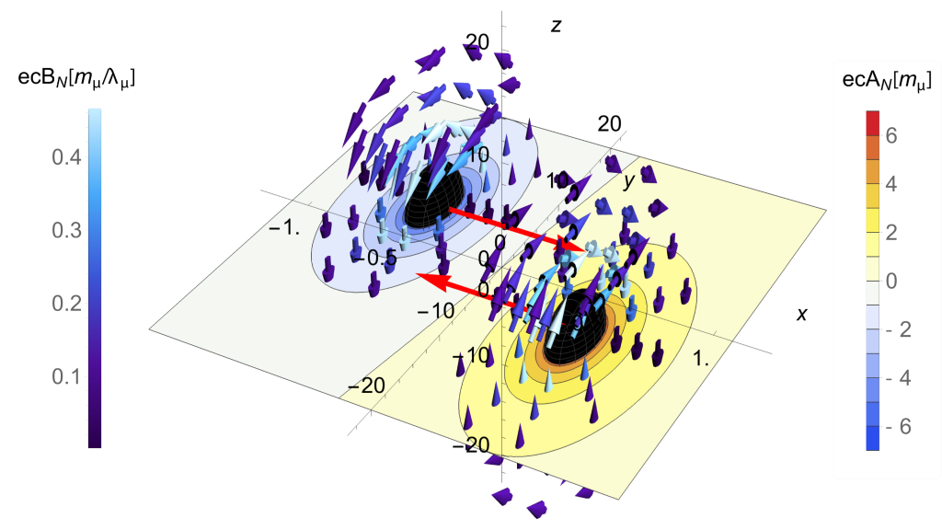
\includegraphics[width=0.85\linewidth]{plots/chap02QCD/Bfield.png}
    \caption{The vacuum magnetic field for two colliding lead Pb nuclei is shown for impact parameter $b=3R$ and $\gamma =37$. (At larger Lorentz factors, a graphical representation is difficult to visualize without scaling the fields with $\gamma$). The vector potential is plotted in the collision plane, and red arrows indicate the direction of the moving nuclei. This plot mainly shows the magnetic field distribution, which is Lorentz contracted along the direction of motion. The magnetic field lines circulate out of the collision plane perpendicular to the velocity, adding together at the collision center.  }
    \label{fig:vacmag}
\end{figure}

The distribution of the vacuum magnetic field given by the Li\'enard-Wiechert fields is plotted in \reff{fig:vacmag}. This is the same magnetic field found by Lorentz boosting the Coulomb field of a nucleus at rest. We neglect the portion of the field that depends on acceleration since it is small for vacuum scattering of heavy nuclei, compared to the field that depends on velocity.

This magnetic field is treated as an external perturbation on the quark-gluon plasma, filling the overlap region between the two nuclei after they collide. For simplicity, the QGP is modeled as an infinite medium so that complications do not arise at the boundary. The temperature of QGP depends strongly on the collision energy of the nuclei. In \cite{Grayson:2022asf} we study Au+Au collisions at $\sqrt{s_{\text{NN}}}=200\,$GeV with QGP temperature $T=300$\,MeV.  After Heavy Ions collide, the conducting QGP medium generates long-range decaying tails or wakefields in the magnetic field that extend far beyond the collision time \cite{Tuchin:2010vs}. The conductivity of QGP determines the strength of these wakefields. We aim to model these fields in QGP using the formulation discussed in Chapter \ref{chap:PlasmaSF}.

\section{EM conductivity of quark-gluon plasma}

Past analytic calculations \cite{Tuchin:2010vs,Deng:2012pc,McLerran:2013hla,Tuchin:2013apa,Gursoy:2014aka,Li:2016tel,Roy:2015kma} solve Maxwell's equations in the presence of static electric conductivity 
\begin{equation}
   \sigma_0 = \frac{m_D^2}{3\kappa}\,,
\end{equation} 
in a  hydrodynamically evolving QGP. For a collisionless plasma $\kappa\rightarrow0$, the conductivity is infinite, and the medium behaves as a perfect conductor. This work introduces the frequency and wavevector dependence of the QGP analytically using the polarization tensor previously obtained in \cite{Formanek:2021blc}.

Numerical calculations \cite{Inghirami:2016iru,Inghirami:2019mkc} have incorporated the dynamical response of QGP by numerically solving the coupled magneto-hydrodynamic equations for a conducting quark-gluon plasma in the presence of the colliding nuclear charges. More recent calculations \cite{Yan:2021zjc,Wang:2021oqq} also incorporate the frequency and wave-vector dependence of QGP response to electromagnetic fields by solving the coupled Vlasov-Boltzmann--Maxwell equations numerically.



\subsection{The Ultrarelativistic EM polarization tensor in QGP}\label{sec:linresp}

In this Section, we review the ultrarelativistic polarization tensor, including damping, for the idealized case where the QGP is infinite, homogeneous, and stationary. This calculation differs from \cite{Formanek:2021blc} only in that we consider three quark species: up, down, and strange. We start with the Vlasov-Boltzmann equation for each quark flavor \req{eq:boltzmanncov} where we assume all quarks collide on a momentum-averaged time scale $\tau_{\text{rel}} = \kappa^{-1}$. The induced current $ j_{\mathrm{ind}}^\mu$ can be written in terms of the phase-space distribution of quarks and anti-quarks as
\begin{equation}\label{eq:current}
   j_{\mathrm{ind}}^\mu(x) = 2 N_c \int (dp)p^\mu \\ \times \sum_{u,d,s} q_f (f_{f}(x,p) - f_{\bar{f}}(x,p))=  4 N_Q e^2 \int (dp)p^\mu \delta f(x,p)\,,
\end{equation}
where  $N_c$ is the number of colors. We sum over the quark flavors with charges $q_f$, and in the final result, we replace $q_f \delta f = \delta f_f$. The result \req{eq:current} differs from that found in the case of an electron-positron plasma by the factor
\begin{equation}
N_Q \equiv N_c\sum_f (q_f/e)^2 = 2\,,
\end{equation}
for three light quark flavors ($u,d,s$).

In the ultrarelativistic limit, neglecting quark masses, one finds the polarization functions \cite{Formanek:2021blc}:
\begin{align}\label{eq:polfuncsUltra}
&\Pi_{\parallel}(\omega,|\boldsymbol{k}|) = m_D^2\frac{\omega^2}{\boldsymbol{k}^2}\left(1 - \frac{\omega \Lambda}{2|\boldsymbol{k}|-i\kappa \Lambda}\right)\,,\\
&\Pi_{\perp}(\omega,|\boldsymbol{k}|) = \frac{m_D^2\,\omega}{4 |\boldsymbol{k}|}\left( \Lambda \left(\frac{\omega'^2}{\boldsymbol{k}^2} - 1\right) - \frac{2\omega'}{ |\boldsymbol{k}|}\right)\,,
\end{align}
where $\Lambda(\omega,\boldsymbol{k})$ is defined as
\begin{align}\label{eq:definitions}
 \Lambda \equiv \ln \frac{\omega'+  |\boldsymbol{k}|}{\omega'- |\boldsymbol{k}|}\,, \quad \text{with} \quad \omega' = \omega+i\kappa\,.
\end{align}
The parallel and transverse polarization functions have the same form as in \cite{Formanek:2021blc} except for an overall factor $N_Q$  as found in \cite{Kapusta:1992fm,Grayson:2022asf}:
\begin{equation}\label{eq:DebyemQCD}
    {m_D}^2_{(\text{EM})} = \sum_{u,d,s} q^2_f T^2 \frac{N_c}{3} = N_Q\frac{e^2T^2}{3} \equiv C_{\text{em}}T^2\,,
\end{equation}
where $C_{\text{em}} =  2e^2/3$. In the following, we will use $m_D$ as short-hand notation for the electromagnetic screening mass since we do not discuss color screening here.
The transverse conductivity $\sigma_{\perp}$, which controls the response of the plasma to magnetic fields, is related to the imaginary part of the transverse polarization function as in \req{eq:sigmaperp}



\subsection{QCD Damping rate in QGP}

The strength of the plasma response to an external magnetic field depends on the quark damping rate $\kappa$ and the electromagnetic screening mass $m_D$. The scale of the collisional quark damping $\kappa$ is much larger than the electromagnetic Debye mass $m_D$ and electromagnetic damping $\kappa_{\text{EM}}$ because it depends on the strong coupling constant $\alpha_s$, not the electromagnetic coupling $\alpha$.

In \cite{Grayson:2022asf}, we use the first-order electromagnetic Debye mass \req{eq:DebyemQCD} to estimate the electromagnetic screening mass $m_D$. The collision rate $\kappa$ is related to the inverse of the mean-free time of quarks in QGP. We adopt a value for $\kappa$ from \cite{Mrowczynski:1988xu} where the mean-free time is given by the product of the parton density in the QGP and the quark-parton transport cross-section, leading to the expression 
\begin{equation}\label{eq:kappadef}
    \kappa(T) = \frac{10}{17\pi} (9 N_f +16) \zeta(3) \alpha_s^2 \ln\left(\frac{1}{\alpha_s}\right) T\,,
\end{equation}

\begin{figure}[h!]
    \centering
    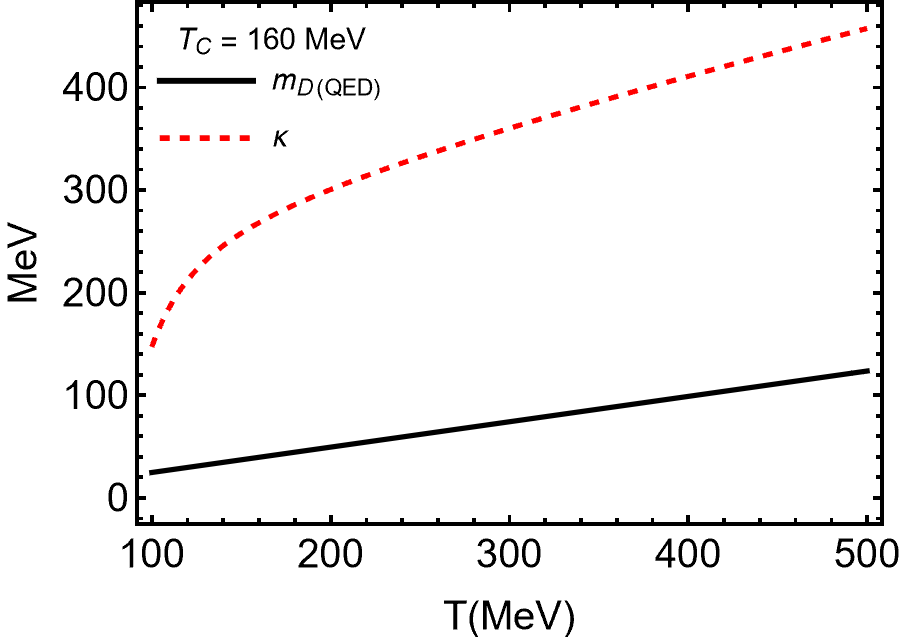
\includegraphics[width=0.85\linewidth]{plots/chap02QCD/kappaDEBYE.png}
    \caption{\textit{From \cite{Grayson:2022asf}.} Plot of the electromagnetic Debye mass and the QCD dampening rate $\kappa$ as a function of temperature. At temperature $T=300\,$MeV used here, $\kappa = 4.86\, m_D$.\label{fig:kappaDebye}}
\end{figure}

where $N_f$ is the number of flavors, $\zeta(x)$ denotes the Riemann zeta function, and $\alpha_s(T)$ is the running QCD coupling.  We model the running of the QCD coupling constant as a function of temperature in the range $T<5T_c$ using a fit provided in \cite{Letessier:2002ony}:
\begin{equation}\label{eq:alphas}
    \alpha_s(T) \approx \frac{\alpha_s(T_c)}{1+C \ln(T/T_c)}\,,
\end{equation}
where $C=0.760 \pm 0.002$. For the QCD (pseudo-)critical temperature we use $T_c = 160\,$MeV. The QED Debye mass is compared to $\kappa(T)$ in Fig.~\ref{fig:kappaDebye}. 
This is plotted along with the electromagnetic Debye mass in \reff{fig:kappaDebye}. We can expect the electromagnetic response of QGP response to be over-damped since $\kappa> \frac{2}{\sqrt{3} m_D}$ giving a plasma frequency \req{eq:plasmafreq} which is imaginary over the range of temperatures relevant for QGP.


\begin{figure}[h!]
    \centering
    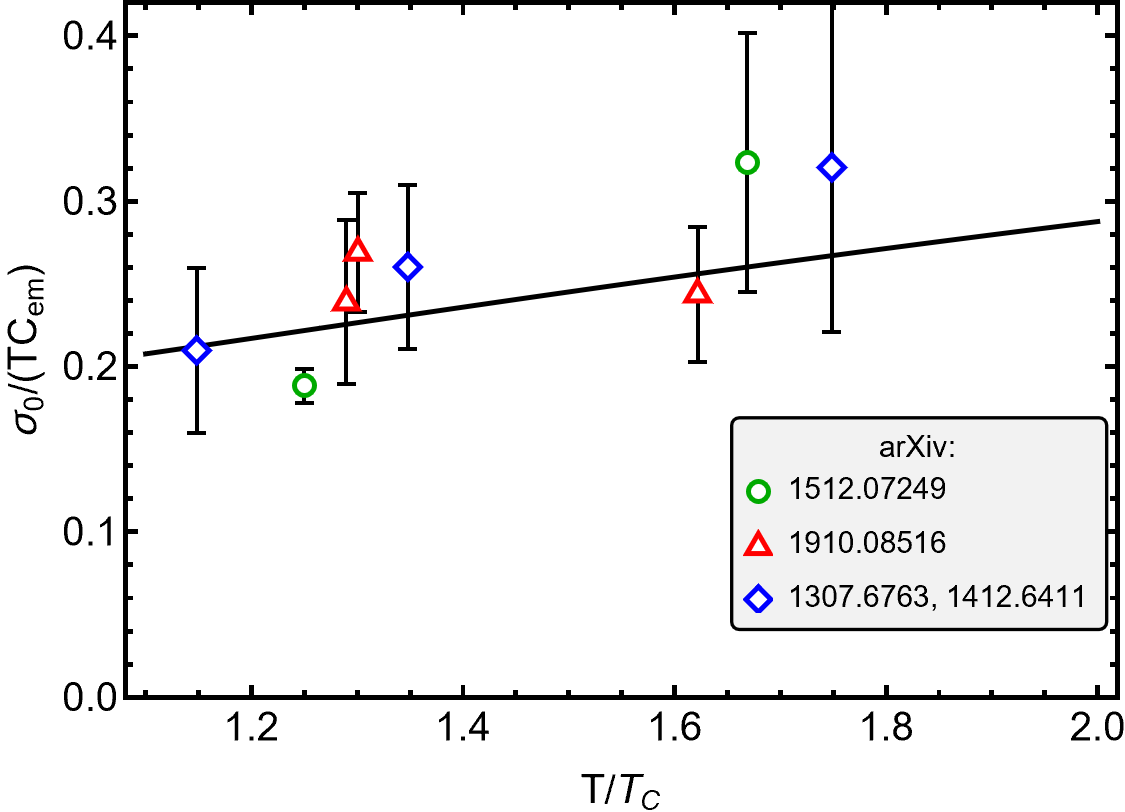
\includegraphics[width=0.85\linewidth]{plots/chap02QCD/condcomp.png}
    \caption{The black line shows the static conductivity $\sigma_0$ as a function of temperature predicted by \req{eq:condstat}, which is compared to lattice results adapted from \cite{Aarts:2020dda} for $T>T_c$. The factor of $C_{\text{em}}$, defined in \req{eq:DebyemQCD}, normalizes the conductivity by the charge of the plasma constituents, such that results using different numbers of dynamical quark flavors can be compared. We indicate each set of points by its arXiv reference: blue diamonds \cite{Amato:2013naa,Aarts:2014nba}, green circles \cite{Brandt:2015aqk}, and red triangles \cite{Astrakhantsev:2019zkr}.}
    \label{fig:lattice comp}
\end{figure}


We can then use the Debye mass \req{eq:DebyemQCD} and the damping rate \req{eq:kappadef} to calculate the static conductivity \req{eq:condstat}, shown as a black line in \reff{fig:lattice comp}, which we then compare to Lattice calculations of the conductivity in QGP.


These lattice-QCD results \cite{Amato:2013naa,Aarts:2014nba,Brandt:2015aqk,Astrakhantsev:2019zkr} are scaled with temperature $T$ to remove the linear temperature dependence. We also scale the conductivity with $C_{\text{em}}$, as defined in \req{eq:DebyemQCD}, such that computations with different numbers of flavors can be compared. One can see that the conductivity value predicted by \req{eq:kappadef}, plotted in Fig.~\ref{fig:lattice comp} as a black line, lies well within the lattice-QCD results. We will use the value predicted by \reff{fig:lattice comp}, $\sigma = 5.01\,$MeV at $T=300\,$GeV, in the next section to compute the screened heavy ion fields in QGP.

% Here, we focus on the damping effect of the collision rate $\kappa$ on the induced magnetic fields in nuclear collisions. The collision term generates a nonvanishing conductivity via the imaginary part of the polarization tensor. This conductivity manifests itself in poles of the resummed propagator in the lower complex $\omega$-plane that generate long-range tails or wake fields that extend far beyond the collision time. In Table~\ref{tab:timescales} we collect the relevant timescales of the problem in ascending order.  The collision time $t_{\text{coll}}$ is much shorter than all other relevant time scales. The collective oscillations of the plasma are highly damped by the large value of the relaxation time giving rise to over-damped behavior.

% \begin{table}[h!]
% \caption{\label{tab:timescales}
% Approximate time scales relevant to the electromagnetic response of QGP for an Au+Au collisions at $\sqrt{s_{\text{NN}}}=200\,$GeV with QGP temperature $T=300$\,MeV. Time scales are shown in ascending order.}
% \begin{ruledtabular}
% \begin{tabular}{ccc}
% \textrm{Time Scale}&
% \textrm{Formula}&
% \multicolumn{1}{c}{\textrm{Time (fm/c)}}\\
% \colrule
%  \textrm{Collision Time} & $t_\text{coll} = 2 R/\gamma$ & 0.086\footnote{Calculated using the Gaussian radius $R = 4.33$\,fm defined in \req{eq:radius}.} \\
% \textrm{Relaxation Time} & $\tau_\text{rel} = 1/\kappa$ & 0.36 \\

% \textrm{Freeze-out time} & $t_f$ & $5$\footnote{Estimated using 2+1 dimensional hydrodynamic evolution \cite{Song:2007ux}.}\\
% \textrm{ Decay Time} & $t_{\sigma} = 1/\sigma_0 = \kappa/\omega_p^2$ & 59\footnote{The decay time is the large damping $\kappa/\omega_p$ expansion of the plasma oscillation frequency \req{eq:plasmafreq}. } \\
% \end{tabular}
% \end{ruledtabular}
% \end{table}



%%%%%%%%%%%%%%%%%%%%%%%%%%%%%%%%%%%%%%%%%%%%%%%%%%%%%%%%%%%%%%%%%%%%%%%%%%%%%%%%%%%%%%%%%%%%%%%%

\section{Magnetic field in QGP during a nuclear collision}\label{sec:Maxwell2}
Assuming that the QGP is an infinite homogeneous and stationary medium near equilibrium, we can solve Maxwell's equations for the self-consistent fields as in Section~\ref{sec:Maxwell}. Then the magnetic field is given by Fourier transforming the momentum space expressions given in \reqs{eq:aperp}{eq:ftfields} to position space
\begin{equation}\label{eq:magorgin}
   \boldsymbol{B}(t, z) = \int \frac{d^4k}{(2\pi)^4}  e^{-i\omega t+ik_z z}
 \frac{\mu_0 i \boldsymbol{k} \times\ft{j}_{\perp \text{ext}}(\omega, \boldsymbol{k})}{\boldsymbol{k}^2 - \omega^2 - \mu_0 \Pi_{\perp}(\omega, \boldsymbol{k})}\,.
\end{equation}
We choose the collision center as the origin of our spatial coordinate system and align the spatial $z$-axis with the beam direction. Due to the symmetry of the colliding ions, the only nonzero component of the magnetic field along the $z$-axis points out of the collision plane ($x-y$ plane). In our coordinate system used in \cite{Grayson:2022asf}, this corresponds to the $y$-component of the magnetic field. 

For ease of calculation, we specify the external 4-current using two colliding Gaussians charge distributions normalized to the nuclear rms radius $R$ and charge $Z$:
\begin{equation}\label{eq:rhoext}
\rho_{\text{ext}\pm }(t,\boldsymbol{x}) = \frac{Zq\gamma}{\pi^{3/2}R^3}e^{-\frac{1}{R^2}(x\mp b/2)^2}e^{-\frac{1}{R^2}y^2}
\times e^{-\frac{\gamma^2}{R^2}(z\mp \beta t)^2}\,,
\end{equation}
where $\gamma$ is the Lorentz factor, $\beta$ is the ratio of the ion speed to the speed of light, respectively, and $b$ is the impact parameter of the collision. The plus and minus signs indicate motion in the $\pm \hat{z}$-direction (beam-axis). This charge distribution corresponds to the vector current
\begin{equation}\label{eq:jext}
\boldsymbol{j}_{\text{ext}\pm}(t, \boldsymbol{x}) = \pm \beta \hatv{z} \rho_{\text{ext}\pm}(t, \boldsymbol{x})\,.
\end{equation}
Further details of the external charge distribution for two colliding nuclei are presented in Appendix B. of \cite{Grayson:2022asf}.

The numerical result for the position-space magnetic field found by Fourier transforming \req{eq:magorgin} using the full transverse polarization function \req{eq:polfuncsUltra} is shown as a red dashed line in Fig.~\ref{fig:bfcomp} and compared with various models of conductivity. These other models and their connections to published works are discussed in detail in \cite{Grayson:2022asf}.

\phantom{Phantom text}
\begin{figure}[h]
\centering              
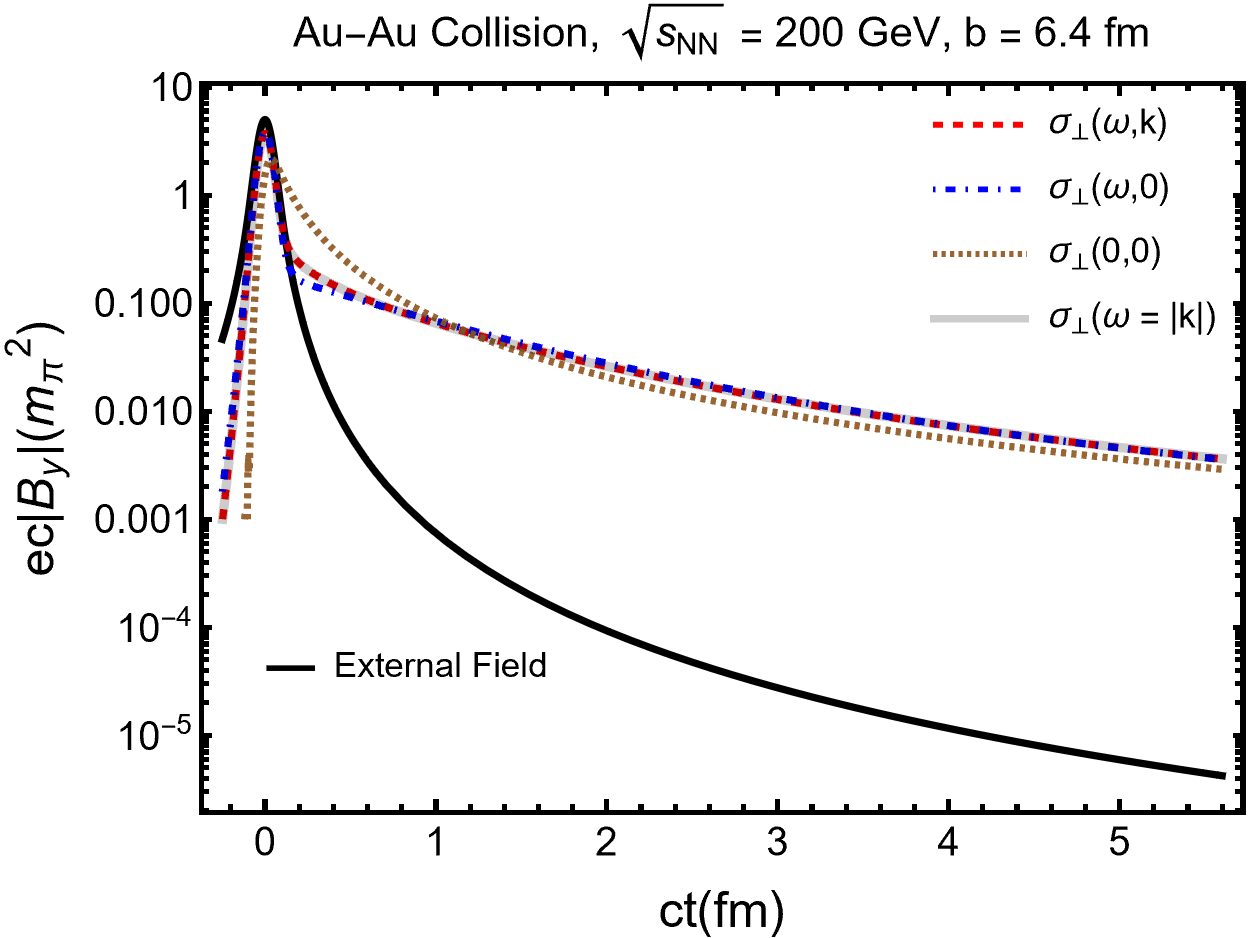
\includegraphics[width=0.46\linewidth]{plots/chap02QCD/bf100.png}
%}
\hspace{0.05\linewidth}
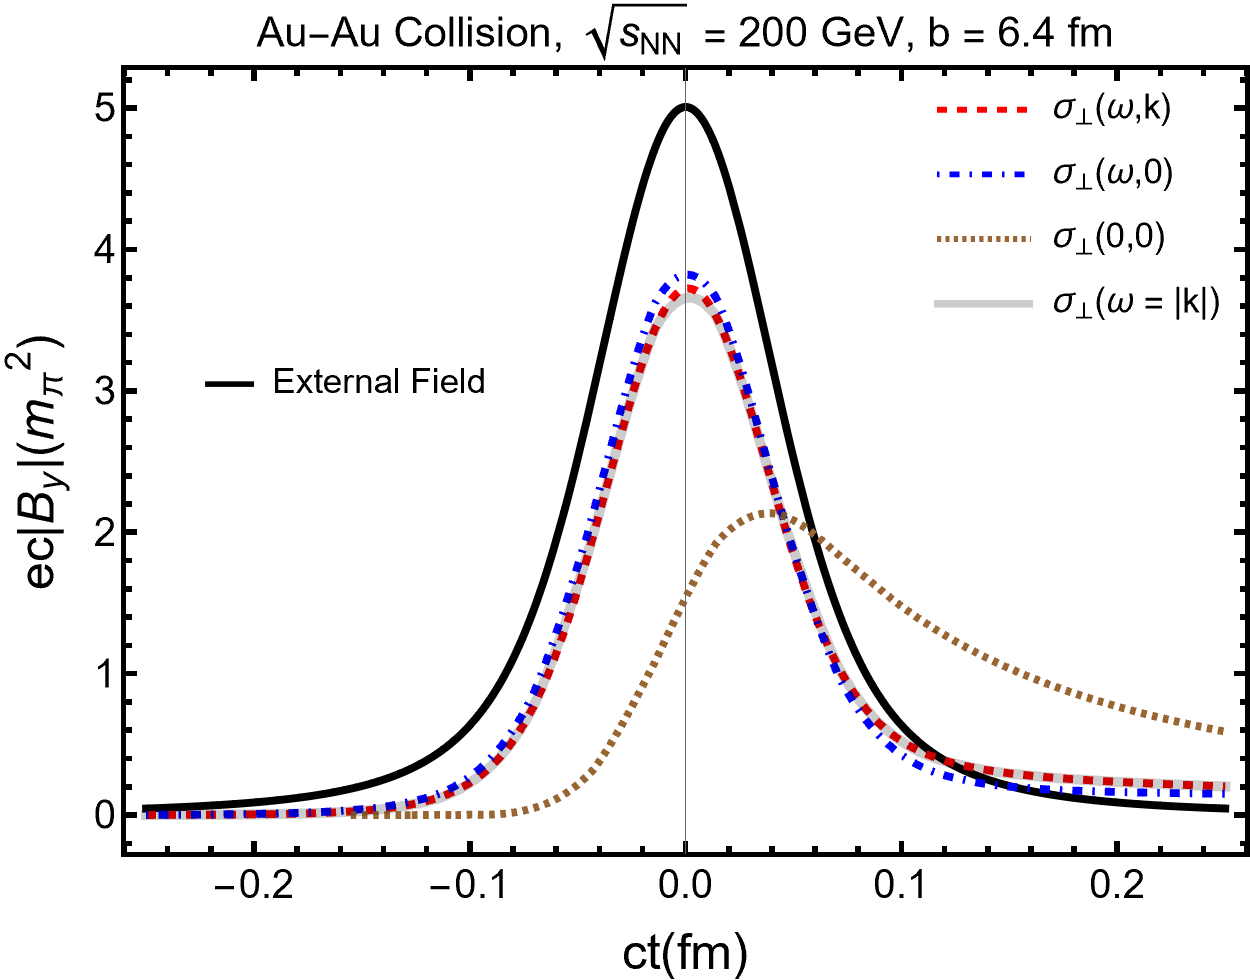
\includegraphics[width=0.44\linewidth]{plots/chap02QCD/bf100lin.png}
%}
\caption{\textit{From \cite{Grayson:2022asf}.} The magnetic field at the collision center as a function of time, with $T = 300$\,MeV for Au-Au collisions ($Z=79$) at $\sqrt{s_\text{NN}} = 200$\,GeV and impact parameter $b = 6.4\,$fm. The left panel shows the magnetic field on a semi-logarithmic scale up to $ct = 5$\,fm. The right panel shows the early-time magnetic field on a linear scale. At the chosen temperature, the electromagnetic Debye mass is $m_D = 74\,$MeV, and the quark damping rate is $\kappa = 4.86\,m_D$. This gives a static conductivity of $\sigma_0 = 5.01\,$MeV. Comparing the different approximations, we see they all have similar asymptotic behavior. Only the Drude conductivity, the light-cone limit of the conductivity, and the full conductivity $\sigma_\perp(\omega,\boldsymbol{k})$ describe the field at early times. Note that the plasma is considered homogeneous and stationary here. In a more realistic situation, the field would become screened only after the QGP is formed in the collision.\label{fig:bfcomp}}
\end{figure}

One of the important results of this paper was that the fields of the ions, traveling near the speed of light, probe the polarization tensor along the light cone. The transverse conductivity on the light cone is
\begin{equation}\label{eq:lightcone}
    \sigma_\perp (\omega = |\boldsymbol{k}|)  =  i \frac{m_D^2}{4 \omega}\left( \frac{\kappa^2}{\omega^2} \xi \ln\xi +\frac{i\kappa}{\omega}\left(\xi+1\right)\right)\,,
\end{equation}
where $\xi$ is defined as
\begin{equation}\label{eq:xidef}
    \xi \equiv 1- 2i \frac{\omega}{\kappa}\,.
\end{equation}
The light-cone conductivity simplifies the calculation of plasma response since it only depends on a single variable ($\omega = |\boldsymbol{k}|$). One can see that \req{eq:lightcone} shown as an opaque grey line traces out the full numerical solution \req{eq:magorgin} shown as a dashed red line. The light-cone conductivity accurately models the magnetic field in QGP since the ions traveling near the light's speed only sample the polarization tensor on the light-cone. One subject of future research is to use the light-cone conductivity to attain analytical formulas for electromagnetic fields in position space in light-cone coordinates.


The simplest method to calculate the late-time magnetic field of colliding nuclei is to assume a static conductivity \cite{Tuchin:2013apa}. In this case, the magnetic field in Fourier space has the form
\begin{equation}\label{eq:bstat}
    \ft{B}(\omega,\boldsymbol{k}) = \frac{ \mu_0 i\boldsymbol{k} \times \ft{j}_{\perp \text{ext}}}{\boldsymbol{k}^2 - \omega^2 - i\omega\sigma_0}\,,
\end{equation}
which is Fourier transformed using contour integration in the appendix of \cite{Grayson:2022asf} to
\begin{equation}\label{eq:banalyticapp}
   B_y(t) = -\mu_0 \frac{ Zq \beta }{(2\pi)} \frac{ b\sigma_0}{4t^2} e^{\frac{-b^2 \sigma_0}{16 t}}\,.
\end{equation}
Looking at the left panel of Fig.~\ref{fig:bfcomp}, the static conductivity initially overestimates the magnetic field after the external field begins to disappear since the effect of dynamic screening is not captured. Every model of the response function predicts similar values for the magnetic field approaching the freeze-out time $t_f \approx 5\,$fm/c \cite{Song:2007ux}. This is because the static conductivity determines the dependence of the magnetic field at times later than $t>1/\sigma \approx 59$\,fm/c after which damping of the initial magnetic field pulse is irrelevant. 

Alternatively, by assuming a point-like charge distribution $R\rightarrow0$ and approximating the magnetic field for $ 1/\sigma_0 > t\gg 1/\kappa$ one can derive the late-time magnetic field using the Drude conductivity \req{eq:drude}
\begin{equation}\label{eq:latetimeB}
   B_y(t) \approx  \mu_0 \frac{ Ze \beta b \kappa \omega_p }{8\pi}\bigg[ \frac{1- e^{-\kappa t}}{\kappa t} - e^{-\kappa t} \text{Ei}\left(t\kappa\right)\bigg]\,.
\end{equation}
This result has the advantage of accurately describing the late-time magnetic field $t>t_f$  at large $\gamma$ as shown in \reff{fig:bcolcomp}.

Both these results illustrate that the late-time magnetic field has a finite limit when $\gamma\rightarrow\infty$ as it depends only on $\beta$, but not on $\gamma$.
\begin{figure}
\centering
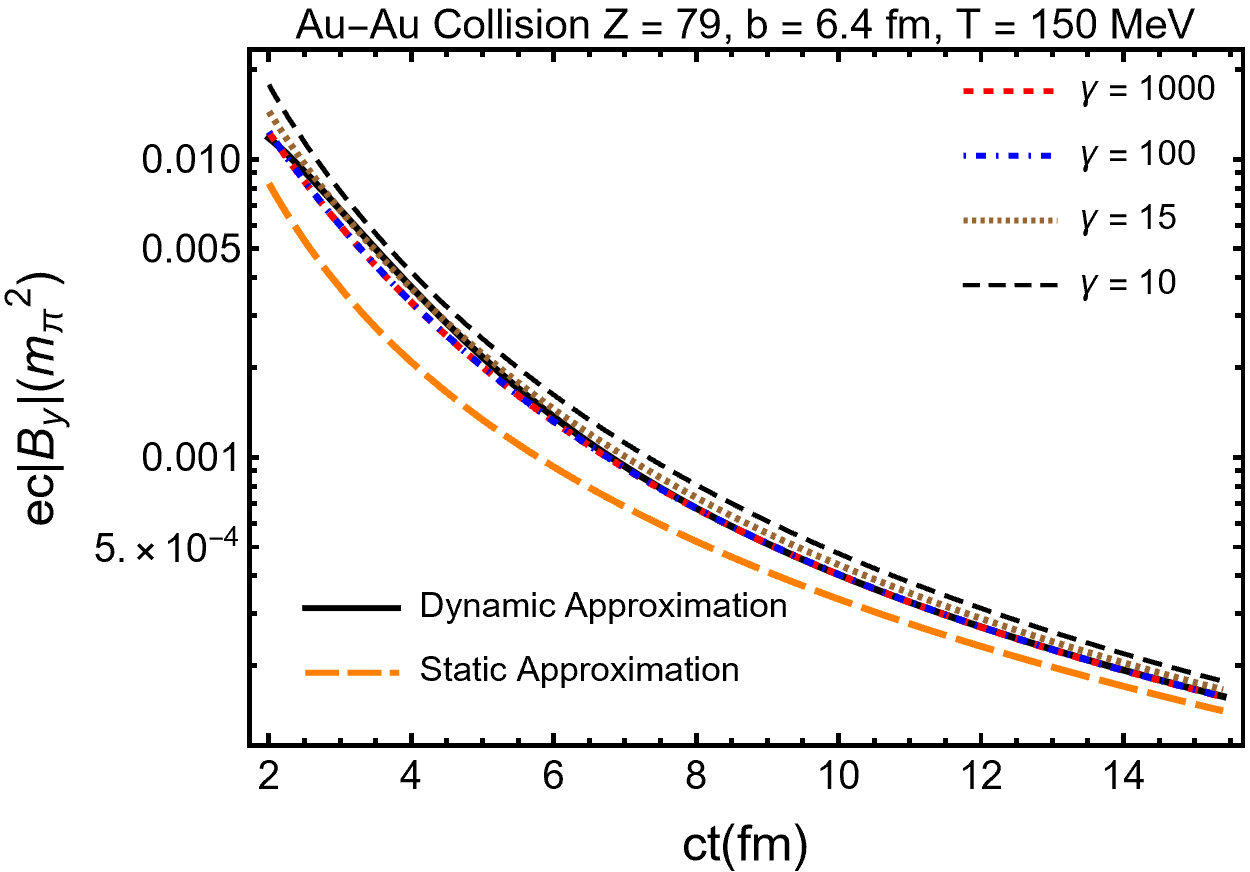
\includegraphics[width=0.85\linewidth]{plots/chap02QCD/bfgaamacomp.png}
    \caption{\textit{Adapted from \cite{Grayson:2022asf}.} Plot of the freeze-out magnetic field for $T= 150$\,MeV. We expect that around this temperature QGP will hadronize into a mixed phase \cite{Letessier:1992xd}. The approximate late time solution \req{eq:banalyticapp} shown as an orange dashed line is compared to numerical calculations using the full polarization tensor \req{eq:magorgin} and to the late time analytic expansion \req{eq:latetimeB}. The approximate solution does not fully match the ultrarelativistic limit until times $t > t_{\sigma} \approx 59$\,fm/c. The magnetic field is independent of the beam energy over a wide range of $\gamma$ but begins to diverge slowly from the ultrarelativistic case at around $\gamma \leq 15$ for the time window shown in the figure. Lower beam energies result in a somewhat larger field at late times.\label{fig:bcolcomp}}
\end{figure}
The approximation used to derive this solution holds for $\gamma\beta \gg \sqrt{ \kappa/\sigma_0} \approx 12$. In Fig.~\ref{fig:bcolcomp} we compare \req{eq:banalyticapp} to the full numerical result to explore its dependence on $\gamma$.  One can see that the static case \req{eq:banalyticapp} (black solid line) begins to diverge from the numerical solution, shown as dashed colored lines at around $\gamma \approx 15$.  In Fig.~\ref{fig:bcolcomp} one can see that the late-time magnetic field has a very soft dependence on collision energy. The time at which hadronization occurs $t_f$, which varies with collision energy, has a much stronger effect on the magnitude of the freeze-out field. Since the remnant magnetic field at hadronization does not depend strongly on the collision energy, an experimental measurement of the magnetic field at different collision energies could permit a determination of the electrical conductivity of the QGP or a determination of the freeze-out time of QGP if the conductivity is assumed to be known. 

As the QGP begins to hadronize at time $t_f$, one may expect hadrons to be statistically polarized with respect to the magnetic field. In \cite{Muller:2018ibh} the measured difference in global polarization of hyperons and antihyperons is used to give an upper bound on the magnetic field at QGP freeze-out, $B \sim 2.7\times 10^{-3}\,m_{\pi}^2$ for Au+Au collisions at $\sqrt{s_\text{NN}} = 200$\,GeV. Looking at Fig.~\ref{fig:bcolcomp} the magnetic field for $\gamma = 100$ at QGP freeze-out $t_f \approx 5 $\,fm/c is predicted to be $B \approx 1.2\times 10^{-3}\,m_{\pi}^2$, somewhat below this upper bound. Note that this assumes the polarization rapidly equilibrates in the plasma. It also neglects any interactions during the hadron gas phase of the collision. 
%%%%%%%%%%%%%%%%%%%%%%%%%%%%%%%%%%%%%%%%%%%%%%%%%%%%%%%%%%%%%%%%%%%%%%%%%%%%%%%%%%%%%%%%%%%%%%%%%%%%%%%%%%%%%%%%%%%%

% \section{The QGP Polarization tensor}\label{sec:linresp}
% \subsection{Derivation of the Polarization tensor}

% In this Section we derive the polarization tensor, including damping, for the idealized case where the QGP is homogeneous and stationary. We follow the derivation presented in \cite{Formanek:2021blc} for the damped polarization tensor of an electron-positron plasma. The calculation differs slightly from \cite{Formanek:2021blc}, since in QGP we consider three quark species: up, down, and strange. We start from the Vlasov-Boltzmann equation for each quark flavor:
% \begin{equation}\label{eq:VBE}
% (p \cdot \partial) f_f(x,p) + q_f F^{\mu\nu} p_\nu \frac{\partial f_f(x,p)}{\partial p^\mu} = (p\cdot u)C_f(x,p)\,,
% \end{equation}
% The collision term $C_f(x,p)$ in the BGK form is given by
% \begin{equation}\label{eq:collision}
%     C_f(x,p) =\kappa_f\left(\eq{f}_f (p)\frac{n_f(x)}{{\eq{n}_f}} - f_f(x,p)\right)\,,
% \end{equation}
% where plasma constituents collide on a momentum-averaged time scale $\tau_{\text{rel}} = \kappa^{-1}$. The collision term is constructed such that \req{eq:VBE} retains current conservation \cite{Bhatnagar:1954zz}. We show in Sect.~\ref{sec:energymomcons} that energy is also conserved for the case of a neutral particle-antiparticle plasma at linear order in the external field.

% The induced current $ j_{\mathrm{ind}}^\mu$ can be written in terms of the phase-space distribution of quarks and anti-quarks as
% \begin{multline}\label{eq:current}
%    j_{\mathrm{ind}}^\mu(x) = 2 N_c \int (dp)p^\mu \\ \times \sum_{u,d,s} q_f (f_{f}(x,p) - f_{\bar{f}}(x,p))\,,
% \end{multline}
% where  $N_c$ is the number of colors, and we sum over the quark flavors with charges $q_f$. One can calculate the induced current for small perturbations away from equilibrium for each quark flavor
% \begin{equation}\label{eq:perturbation}
% f_f(x,p) = {\eq{f}_f}(p) + \delta f_f(x,p)\,,
% \end{equation}
% Note that the equilibrium contributions ${\eq{f}_f}(p)$ do not contribute to \req{eq:current} because of the opposite sign of the charges of particles and antiparticles, but the perturbations $\delta f$ add up due the change in sign of the external force $qF^{\mu\nu}p_\nu$:
% \begin{multline}\label{eq:current2}
%     j_{\mathrm{ind}}^\mu(x) = 2 N_c \int (dp)p^\mu \sum_{u,d,s} q_f (\delta f_{f}(x,p) - \delta f_{\bar{f}}(x,p))\\
%  = 4 N_c \int (dp)p^\mu \sum_{u,d,s} q_f^2 \delta f(x,p)\\
%   =  4 N_Q e^2 \int (dp)p^\mu \delta f(x,p)\,.
% \end{multline}
% In the second line we pulled out a factor of electric charge $\delta f_{f} = q_f \delta f$. The perturbations $\delta f$ are identical for all quark species in the ultrarelativistic limit. The result \req{eq:current2} differs from that found in the case of an electron-positron plasma by the factor
% \begin{equation}
% N_Q \equiv N_c\sum_f (q_f/e)^2 = 2\,,
% \end{equation}
% where the numerical value holds for three light quarks flavors ($u,d,s$). We refer to \cite{Formanek:2021blc} for the derivation of the polarization tensor in terms of integrals over the phase-space distribution $\delta f$, because the only difference is the overall factor $N_Q$.

% As noted in the previous Section, the polarization tensor in \req{eq:poltensgen} may be written in terms of two independent components: the longitudinal polarization function $\Pi_{\parallel}$, which describes response parallel to wave-vector $\boldsymbol{k}$, and the transverse polarization function $\Pi_{\perp}$, which describes response in the plane perpendicular to wave-vector $\boldsymbol{k}$. When the $\mu=3$ ($z$) axis is chosen along the wave-vector $\boldsymbol{k}$, the longitudinal and transverse polarization functions relate to the components of the polarization tensor \req{eq:poltenmat} along the coordinate axes as
% \begin{equation}\label{eq:piLT}
%     \Pi_{\parallel} =\Pi^3_3, \quad \Pi_{\perp} =\Pi^1_1=\Pi^2_2\,.
% \end{equation}
% In the ultrarelativistic limit, neglecting quark masses, one finds \cite{Formanek:2021blc}:
% \begin{align}\label{eq:polfuncs}
% &\Pi_{\parallel}(\omega,|\boldsymbol{k}|) = m_D^2\frac{\omega^2}{\boldsymbol{k}^2}\left(1 - \frac{\omega \Lambda}{2|\boldsymbol{k}|-i\kappa \Lambda}\right)\,,\\
% &\Pi_{\perp}(\omega,|\boldsymbol{k}|) = \frac{m_D^2\,\omega}{4 |\boldsymbol{k}|}\left( \Lambda \left(\frac{\omega'^2}{\boldsymbol{k}^2} - 1\right) - \frac{2\omega'}{ |\boldsymbol{k}|}\right)\,,
% \end{align}
% where $\Lambda(\omega,\boldsymbol{k})$ is defined as
% \begin{align}\label{eq:definitions}
%  \Lambda \equiv \ln \frac{\omega'+  |\boldsymbol{k}|}{\omega'- |\boldsymbol{k}|}\,, \quad \text{with} \quad \omega' = \omega+i\kappa.
% \end{align}
% The natural logarithm leads to branch cut in the complex $\omega$ plane running from $-|\boldsymbol{k}|-i\kappa$ to  $|\boldsymbol{k}|-i\kappa$ as noted in \cite{Romatschke:2015gic}. The parallel and transverse polarization functions have the same form as in \cite{Formanek:2021blc} except for an overall factor $N_Q$ that is contained in the leading order electromagnetic Debye mass for the QGP plasma \cite{Kapusta:1992fm}:
% \begin{equation}\label{eq:DebyemQCD}
%     {m_D}^2_{(\text{EM})} = \sum_{u,d,s} q^2_f T^2 \frac{N_c}{3} = N_Q\frac{e^2T^2}{3} \equiv C_{\text{em}}T^2\,,
% \end{equation}
% where $C_{\text{em}} =  2e^2/3$. In the following we will use $m_D$ as short-hand notation for the electromagnetic screening mass since we do not discuss color screening here.

% The polarization tensor may be written in any general frame by using \req{eq:poltensgen}, but for our purposes it will be simpler to carry out calculations in the coordinate system where $\boldsymbol{k}$ aligns with the $z$-axis so that the polarization tensor takes the form shown in \req{eq:poltenmat}.


%  \subsection{QGP parameters}
 
% The strength of the plasma response to an external magnetic field depends on the values of two physical parameters: the quark damping rate $\kappa$, and the electromagnetic screening mass $m_D$. In this Section we provide estimates for these parameters. 

% We adopt the perturbative result \req{eq:DebyemQCD} to estimate $m_D$. Higher-order corrections to this expression can been derived from higher-order calculation of the vector spectral function in thermal perturbation theory (see \cite{Jackson:2019mop} and references cited therein).

% The scale of the collisional quark damping $\kappa$ is much larger than the electromagnetic Debye mass $m_D$ because it depends on the strong coupling constant $\alpha_s$, not the electromagnetic coupling $\alpha$. Solving the dispersion relation
% \begin{equation}
%     \frac{1}{(k\cdot u)^2}(k^2+ \mu_0\Pi_\parallel(\omega, k))(k^2 + \mu_0 \Pi_\perp(\omega, k))^2=0 \,,
% \end{equation}
% see \cite{melrose2008quantum}, in the limit $\boldsymbol{k}\rightarrow 0$ one finds for the plasma oscillation frequency \cite{Formanek:2021blc}
% \begin{equation}\label{eq:plasmafreq}
%     \omega_{p}^\pm = -\frac{i\kappa}{2} \pm \sqrt{\frac{m_D^2}{3} - \frac{\kappa}{4}^2}\,.
% \end{equation}
% We see that if $\kappa > \tfrac{2}{\sqrt{3}}m_D $, the plasma oscillations are over-damped.

% \begin{figure}[h!]
%     \centering
%     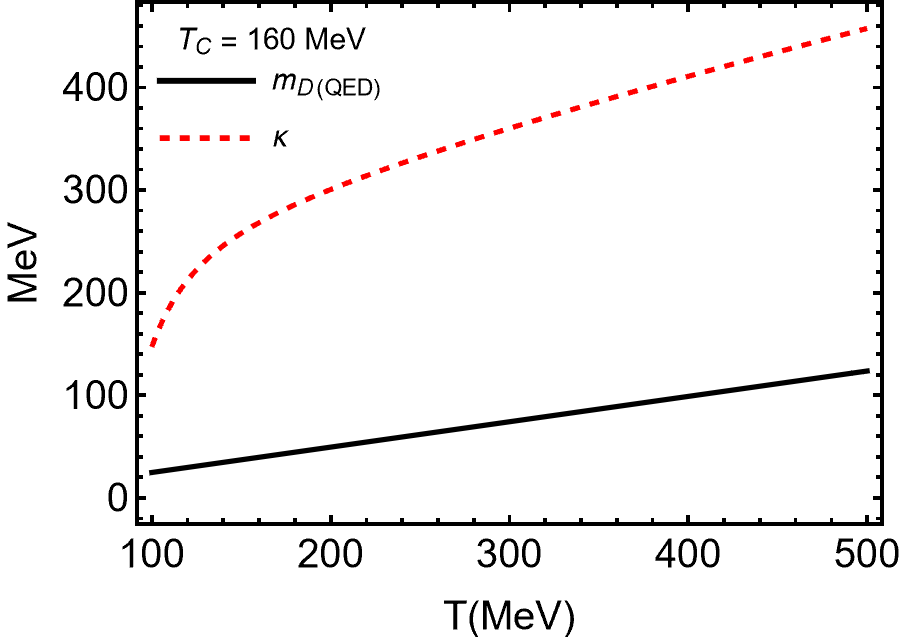
\includegraphics[width=0.85\linewidth]{plots/chap02QCD/kappaDEBYE.png}
%     \caption{Plot of the QED Debye mass and the QCD dampening rate $\kappa$ as a function of temperature. At temperature $T=300\,$MeV used in the plots below, $\kappa = 4.86\, m_D$.\label{fig:kappaDebye}}
% \end{figure}

% The collision rate $\kappa$ is related to the inverse of the mean-free time of quarks in QGP. In kinetic theory the mean-free time is given by the product of the parton density in the QGP and the quark-parton transport cross section, leading to the expression \cite{Mrowczynski:1988xu}
% \begin{equation}\label{eq:kappadef}
%     \kappa(T) = \frac{10}{17\pi} (9 N_f +16) \zeta(3) \alpha_s^2 \ln\left(\frac{1}{\alpha_s}\right) T\,,
% \end{equation}
% where $N_f$ is the number of flavors, $\zeta(x)$ denotes the Riemann zeta function, and $\alpha_s(T)$ is the running QCD coupling.  We model the running of the QCD coupling constant as a function of temperature in the range $T<5T_c$ using a fit provided in \cite{Letessier:2002ony}:
% \begin{equation}\label{eq:alphas}
%     \alpha_s(T) \approx \frac{\alpha_s(T_c)}{1+C \ln(T/T_c)}\,,
% \end{equation}
% where $C=0.760 \pm 0.002$. For the QCD (pseudo-)critical temperature we use $T_c = 160\,$MeV. The QED Debye mass is compared to $\kappa(T)$ in Fig.~\ref{fig:kappaDebye}. 

% From $\kappa(T)$ in \req{eq:kappadef} and the running of the coupling in \req{eq:alphas}, we calculate the static conductivity using the leading order electromagnetic Debye mass $m_D$. The momentum dependent transverse conductivity $\sigma_{\perp}$, which controls the response of the plasma to magnetic fields, is related to the imaginary part of the transverse polarization function $\Pi_{\perp}$ as follows \cite{melrose2008quantum}:
% \begin{equation}\label{eq:conddef}
%     \sigma_{\perp}(\omega,\boldsymbol{k}) = -i \frac{\Pi_{\perp}(\omega,\boldsymbol{k})}{\omega}\,.
% \end{equation}
% In the long wavelength limit $\boldsymbol{k}\rightarrow0$, the branch cut in \req{eq:definitions} shrinks to a single pole at $\omega = -i \kappa$, and the conductivity has the simple form
% \begin{equation}\label{eq:conddrude}
%     \sigma_{\perp}(\omega, 0 ) = \sigma_{\parallel}(\omega, 0 ) = \frac{\sigma_0}{1-i\omega/\kappa}\,.
% \end{equation}
% We will refer to $\sigma_{\perp}(\omega, 0 )$ as the Drude model \cite{Drude:1900}. In the static limit $\omega\rightarrow0$ the parallel and perpendicular conductivities are the same, and the static conductivity $\sigma_0$ is given by
% \begin{equation}\label{eq:condstat}
%    \sigma_0 = \frac{m_D^2}{3\kappa}\,.
% \end{equation} 
%  The static conductivity determines the late time behavior of the magnetic field.

% %%%%%%%%%%%%%%%%%%%%%%%%%%%%%%%%%%%%%%%%%%%%%%%%%%%%%%%%%%%%%%%%%%%%%%%%%%%%%%%%%%%%%%%%%

% \subsection{Energy-momentum conservation}\label{sec:energymomcons}

% In general, the modified BGK collision term \req{eq:collision} violates energy and momentum conservation. Rocha {\it et al.} \cite{Rocha:2021zcw} recently showed how energy-momentum conservation can be restored by introducing a linearized collision operator that is projected on eigenfunctions of the conserved quantities with eigenvalue zero. Here we show explicitly that for a symmetric particle-antiparticle plasma the energy momentum violations cancel at linear order in the external field. 

% Recall that the energy momentum tensor $T^{\mu\nu}$ of the plasma is given by
% \begin{equation}
%     T^{\mu \nu} = 2 \int (dp) p^{\mu} p^{\nu} (f_-(x,p) + f_+(x,p) )\,,
% \end{equation}
% where the factor of two accounts for spin and $f_\pm(x,p)$ represent the distributions of particles ($+$) and antiparticles ($-$), respectively. We recall that for $T^{\mu\nu}$ to be conserved the covariant divergence 
% \begin{equation}
%     \partial_{\mu} T^{\mu \nu} = 2\,\partial_{\mu} \int (dp)p^{\mu} p^{\nu}\left(f_-(x,p) + f_+(x,p)\right)
% \end{equation}
% must vanish. In linear response the distribution functions $ f_{\pm} (x,p)$ are given by
% \begin{equation}
%     f_{\pm} (x,p) = \delta  f_{\pm} (x,p) + \eq{f}(p)\,.
% \end{equation}
% Equation \req{eq:current2} indicates that the perturbation $ \delta  f_{\pm}$ is linear in the quark charge
% \begin{equation}
%     \delta f_\pm = \pm q\, \delta f\,.
% \end{equation}
% This leads to a cancellation of the particle and antiparticle perturbations in the energy-momentum tensor at linear order:
% \begin{equation}
%     \partial_{\mu} T^{\mu \nu} = 4\,\partial_{\mu}\left( \int (dp)p^{\mu} p^{\nu}\eq{f}(p)\right) = 0\,.
% \end{equation}
% Thus for a symmetric particle-antiparticle plasma corrections to the energy-momentum tensor appear only at second order in external field. This is a general consequence of CPT symmetry of the medium. 


% %%%%%%%%%%%%%%%%%%%%%%%%%%%%%%%%%%%%%%%%%%%%%%%%%%%%%%%%%%%%%%%%%%%%%%%%%%%%%%%%%%%%%%%%%%%%%%%%%%%


% \section{Magnetic field in a nuclear collision}\label{sec:results}

% In this Section we calculate the magnetic field at the center of the heavy ion collision by Fourier transforming the momentum space magnetic field \req{eq:ftfields} to position space. We calculate the self-consistent magnetic field using the potentials given in \reqs{eq:phi}{eq:aperp} and model the response of QGP using the idealized case of a homogeneous, stationary plasma detailed in Sects.~\ref{sec:Maxwell2} and \ref{sec:linresp}. The external fields are specified by the moving Gaussian charge distributions defined in \reqs{eq:rhoext}{eq:jext}.

% The magnetic field is of particular interest due to its role in the separation of electric charge in the QGP through the chiral magnetic effect (CME) \cite{Kharzeev:2007jp}. In the large magnetic fields that occur in heavy ion collisions the electric current generated by the CME could lead to a charge separation along the direction of the magnetic field. Whether this effect is observable depends strongly on the size of the magnetic field. If a magnetic field of meaningful strength survives until the time of hadronization of the QGP, it could also lead to a difference in the global polarization of $\Lambda$ hyperons and antihyperons \cite{Muller:2018ibh}.

% We chose the collision center as the origin of our spatial coordinate system and align the spatial $z$-axis with the beam direction. We calculate the magnetic field along the $z$-axis by Fourier transforming the momentum space expressions given in \reqs{eq:aperp}{eq:ftfields}:
% \begin{multline}\label{eq:magorgin}
%    \boldsymbol{B}(t, z) = \int \frac{d^4k}{(2\pi)^4}  e^{-i\omega t+ik_z z}
%  \frac{\mu_0 i \boldsymbol{k} \times\ft{j}_{\perp \text{ext}}(\omega, \boldsymbol{k})}{\boldsymbol{k}^2 - \omega^2 - \mu_0 \Pi_{\perp}(\omega, \boldsymbol{k})}
% \end{multline}
% to position space. It is convenient to perform the Fourier integrals in cylindrical coordinates $(\boldsymbol{x}_\perp,z)$. The angular integral $d\theta$ and the integral over momentum along the beam axis $d k_z $ can be performed exactly. The $d k_z $ integral is trivial due to the delta function in the external charge distribution \req{eq:extchgfreq}. The frequency integral $d\omega$ and the transverse momentum integral $dk_\rho$ must, in general, be done numerically. We present the details of this calculation in Appendix \ref{sec:magf}. Due to the symmetry of the colliding ions, the only nonzero component of the magnetic field along the $z$-axis points out of the collision plane ($x-y$ plane). In our coordinate system, described in Appendix \ref{sec:freechg}, this corresponds to the $y$-component of the magnetic field. The numerical results for the position-space magnetic field are shown in Fig.~\ref{fig:bfcomp} and compared with earlier results.

% To connect to these previous studies, we compute the magnetic field in position space at the origin in various levels of approximation defined in \reqs{eq:conddef}{eq:condstat} and \req{eq:lightcone}.
% \begingroup
% \renewcommand{\arraystretch}{1.5} % Default value: 1
% \begin{table}[b]
% \caption{\label{tab:cond}
% Conductivity models used to calculate the resulting magnetic field. Each conductivity represents the response of QGP with a different spacetime dependence. }
% \begin{ruledtabular}
% \begin{tabular}{ccc}
% \textrm{Conductivity}&
% \textrm{Dependence}&
% \multicolumn{1}{c}{\textrm{Formula}}\\
% \colrule
%  \textrm{Full} & $\sigma_{\perp}(\omega,\boldsymbol{k})$ & $-i \Pi_{\perp}(\omega,\boldsymbol{k})/\omega$  \\
%  \textrm{Light-cone} & $\sigma_{\perp}(\omega = |\boldsymbol{k}|)$ & \req{eq:lightcone}  \\
% \textrm{Drude} & $\sigma_{\perp}(\omega, 0 )$ & $\sigma_0/(1-i\omega/\kappa)$ \\
% \textrm{Static} & $\sigma_0$ & $m_D^2/(3\kappa)$ \\
% \end{tabular}
% \end{ruledtabular}
% \end{table}
% \endgroup
% These conductivities, collected in Table\,\ref{tab:cond}, refer to different treatments of the frequency $\omega$ and wave-vector $\boldsymbol{k}$ dependence of the conductivity $\sigma_\perp(\omega, \boldsymbol{k})$. For instance, solving for the magnetic field in the limit $\boldsymbol{k}\rightarrow0$ assumes that the spatial dependence of the external field can be neglected, not superficially a good approximation because at any given time $t$ the field varies rapidly with $z$.  The levels of approximation we consider include: the full space- and time-dependence of the conductivity $\sigma_\perp(\omega, \boldsymbol{k})$, the Drude model \req{eq:conddrude}, and the static response $\sigma_\perp(0,0)$. We list these limits in \reqs{eq:conddef}{eq:condstat}, respectively. 

% The fourth limit we are considering is the conductivity along the light-cone $\sigma_\perp(\omega,k_z=\pm\omega,k_\rho=0)$. We now show that the light-cone limit closely resembles the Drude model. We first recall that the frequency dependence of the free charge distribution in cylindrical coordinates \req{eq:extchgfreq} has the form
% \begin{multline}
% \wt{\rho}_{\text{ext}\pm}(\omega,\boldsymbol{k}) = 2\pi Zq\, e^{-(k_{\rho}^2 + k_z^2/\gamma^2)\frac{R^2}{4}} \\
% \times e^{\mp \frac{ik_{\rho} b \cos\theta }{2}} \delta(\omega \mp k_z \beta)\,.
% \end{multline} 
% After performing the Fourier transform over the parallel component of the wave-vector $k_z$ using the delta function, the magnitude of the wave-vector $|\boldsymbol{k}|$ is effectively set to the light-cone $\omega \approx |\boldsymbol{k}|$, with a small deviation due to the transverse dependence of the field,
% \begin{equation}
%     |\boldsymbol{k}|^2 = k_z^2+ k_{\rho}^2 \rightarrow  (\omega/\beta)^2+ k_{\rho}^2\,.
% \end{equation}
% Inspecting the external charge distribution after this replacement
% \begin{multline}
% \wt{\rho}_{\text{ext}\pm}(\omega,k_{\rho}) = 2\pi Zq\, e^{-(k_{\rho}^2 + \omega^2/(\beta \gamma)^2)\frac{R^2}{4}} \\
% \times e^{\mp \frac{ik_{\rho} b \cos\theta }{2}}\,,
% \end{multline}
% we can see that the size of the deviation from the light-cone due to $k_{\rho}$ is or order $O(1/R)$, while the width of the current distribution in frequency space is of order $O(\beta\gamma/R)$.
% \begin{figure}[h!]
%     \centering
%     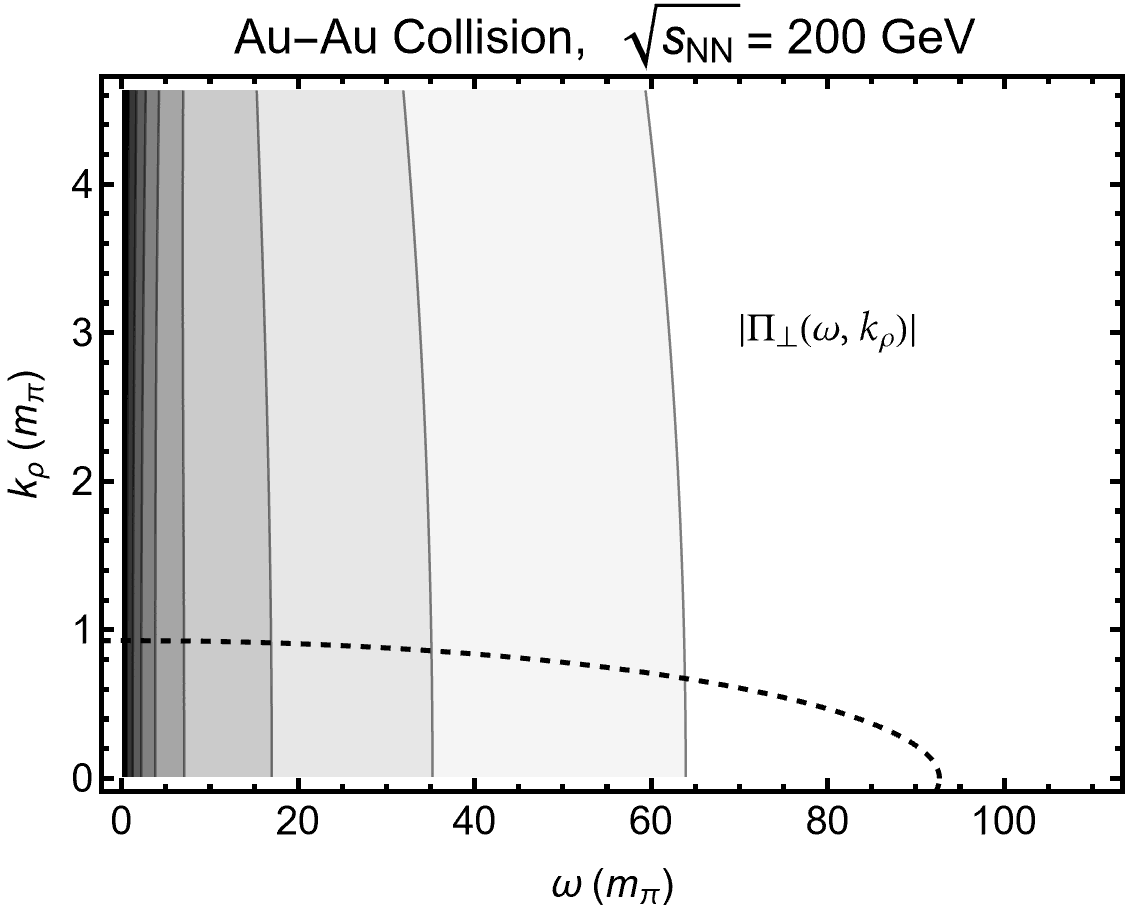
\includegraphics[width=0.85\linewidth]{plots/chap02QCD/lightcone2.png}
%     \caption{The magnitude of the polarization tensor is plotted in momentum space showing deviations in $k_\rho$ from the light-cone $\omega = |\boldsymbol{k}|$ on the horizontal axis. The contours show lines of constant magnitude of $\Pi_\perp(\omega, |\boldsymbol{k}|)$; lighter shading indicates increasing magnitude. The dashed line encapsulates the $2\sigma$ support of the external charge distribution. The width of the external charge distribution in momentum space is $\sqrt{2}/R$ in the transverse direction and  $\beta \gamma \sqrt{2}/R$ along the light-cone. One can see that in the region sampled by the external charge distribution the polarization tensor is effectively constant as a function of $k_\rho$. \label{fig:lightcone}}
% \end{figure} 
% The region of two-sigma support of the Gaussian charge distribution is shown as the region enclosed by the dashed line in Fig.~\ref{fig:lightcone}. The polarization tensor is approximately constant as a function of $k_\rho$ in this region. This implies that one can approximate the integral in \req{eq:magorgin} using the polarization function at $k_\rho = 0$, i.~e.\, on the light-cone. This means that the fields of the ions, traveling near the speed of light, probe the polarization tensor along the light-cone. In this limit, the transverse conductivity near the light-cone is
% \begin{equation}\label{eq:lightcone}
%     \sigma_\perp (\omega = |\boldsymbol{k}|)  =  i \frac{m_D^2}{4 \omega}\left( \frac{\kappa^2}{\omega^2} \xi \ln\xi +\frac{i\kappa}{\omega}\left(\xi+1\right)\right)\,,
% \end{equation}
% where $\xi$ is defined as
% \begin{equation}\label{eq:xidef}
%     \xi \equiv 1- 2i \frac{\omega}{\kappa}\,.
% \end{equation}
% Since the light-cone conductivity only depends on a single variable ($\omega = |\boldsymbol{k}|$) it simplifies integrals involved in the Fourier transform of fields back into position space.

% Our results for the magnetic field at the collision center $B_y(t,0)$ are shown in Fig.~\ref{fig:bfcomp}. The right panel of the figure shows the field at early times ($|t| < 0.25~\text{fm}/c$) on a linear scale, the left panel shows the field over a wider time range on a logarithmic scale. The most general case $\sigma_\perp(\omega, \boldsymbol{k})$, shown as the dashed red curve in Fig.~\ref{fig:bfcomp}, includes the full time- and space-dependent response of the medium to the fields of the colliding ions. The blue dashed curve shows the magnetic field in the  Drude model approximation \req{eq:conddrude}, where the response depends only on time. The magnetic field using the light-cone conductivity is seen as the gray line overlapping the red dashed line in Fig.~\ref{fig:bfcomp},  where $\sigma_0$ is defined in \req{eq:condstat}. The result of Fourier transforming this expression is shown as the brown dotted curve in Fig.~\ref{fig:bfcomp}. Our results differ slightly from those of \cite{Tuchin:2013apa} because here we account for the finite size of the ions and use a slightly different conductivity value. 

% \phantom{Phantom text}
% \begin{figure}[htb]
% \centering
% \includegraphics[width=0.46\linewidth]{plots/chap02QCD/bf100.png}
% %}
% \hspace{0.05\linewidth}
% \includegraphics[width=0.44\linewidth]{plots/chap02QCD/bf100lin.png}
% %}
% \caption{The magnetic field at the collision center as a function of time, with $T = 300$\,MeV for a Au-Au collisions ($Z=79$) at $\sqrt{s_\text{NN}} = 200$\,GeV and impact parameter $b = 6.4\,$fm. The left panel shows the magnetic field on a semi-logarithmic scale up to $ct = 5$\,fm. The right panel shows the early-time magnetic field on a linear scale. At the chosen temperature the electromagnetic Debye mass is $m_D = 74\,$MeV and the quark damping rate is $\kappa = 4.86\,m_D$. This gives a static conductivity of $\sigma_0 = 5.01\,$MeV. Comparing the different approximations we see that all of them have similar asymptotic behavior. Only the Drude conductivity, the light-cone limit of the conductivity, and the full conductivity $\sigma_\perp(\omega,\boldsymbol{k})$ describe the field at early times. Note that here that the plasma is considered homogeneous and stationary. In a more realistic situation the field would become screened only after the QGP is formed in the collision.\label{fig:bfcomp}}
% \end{figure}

% The magnetic field in the presence of a QGP was previously calculated using a static conductivity in \cite{Tuchin:2013apa}. In this case, the magnetic field in Fourier space has the form
% \begin{equation}\label{eq:bstat}
%     \ft{B}(\omega,\boldsymbol{k}) = \frac{ \mu_0 i\boldsymbol{k} \times \ft{j}_{\perp \text{ext}}}{\boldsymbol{k}^2 - \omega^2 - i\omega\sigma_0}\,,
% \end{equation}

% Looking at the left panel of Fig.~\ref{fig:bfcomp}, one can see that every model of the response function predicts similar values for the magnetic field approaching the freeze-out time $t_f$. This is because the static conductivity determines the late-time dependence of the magnetic field. As we discuss in Appendix \ref{sec:magf}, we can expect the static solution to match the full solution when $t > 1/\kappa$. The static conductivity initially overestimates the magnetic field after the external field begins to fall, since the effect of dynamic screening is not captured. This matches the qualitative picture given by the detailed numerical transport calculation done in \cite{Wang:2021oqq}. The full space-time dependent model and the Drude model model behave similarly for most times, and are almost identical for $t>1/\kappa \approx 0.36$\,fm/c. The magnetic field calculated using the polarization tensor evaluated on the light cone tracks the general solution at all times.

% We can use the light-cone conductivity in \req{eq:lightcone} to understand why the Drude model $\sigma_\perp(\omega, 0)$ matches the full solution for times $t>1/\kappa$. Late times probe the small frequency limit of the conductivity. An expansion of \req{eq:lightcone} in $\omega/\kappa$ yields
% \begin{multline}
% \sigma_\perp (\omega = |\boldsymbol{k}|)   = \sigma_0\left(1+i\omega/\kappa\right)\\
% - \frac{6 \sigma_0}{5 }\frac{\omega^2}{\kappa^2}+O\left(\frac{\omega^3}{\kappa^3}\right)\,.
% \end{multline}
% We then compare to the same expansion for the Drude conductivity
% \begin{multline}
% \sigma_\perp (\omega,0) = \frac{\sigma_0}{1- i\omega/\kappa}  \approx  \sigma_0\left(1+i\omega/\kappa\right) \\
% - \sigma_0 \frac{\omega^2}{\kappa^2}+O\left(\frac{\omega^3}{\kappa^3}\right)\,.
% \end{multline}
% The lowest-order term, which coincides with the expression for the Drude model, closely approximates the full solution when $\kappa \gg \omega$ as shown in Fig~\ref{fig:condlightcomp}. Since $\kappa t_f \gg 1$ for the QGP, the series converges rapidly for times of the order of the freeze-out time $t_f$. 
% \begin{figure}[h!]
%     \centering
%     \includegraphics[width=0.85\linewidth]{plots/chap02QCD/condlightcomp.png}
%     \caption{Comparison of the conductivity on the light-cone to $ \sigma_{\perp}(\omega,\boldsymbol{k}\rightarrow 0) $, scaled with the static conductivity. We see that at small $\omega/\kappa$, i.e. times much larger than $1/\kappa$, both approximations converge to the static case, while they diverge $\omega/\kappa > 1$. This predicts that the Drude model will underestimate screening at small times, which is exactly what we observe in Fig.~\protect\ref{fig:bfcomp}. \label{fig:condlightcomp}}
% \end{figure} 

% The simple form of the Drude approximation \req{eq:conddrude} allows one to find the poles of the denominator in \req{eq:magorgin}, analytically. The frequency integral can then be done using the residue theorem, allowing for an approximate analytical expression for the late-time magnetic field. This is done in Appendix \ref{sec:magf}. 
% In the ultrarelativistic limit $\gamma\gg 1$ and large times $t\gg 1/\kappa$ gives
% \begin{equation}\label{eq:banalyticapp}
%    B_y(t) = -\mu_0 \frac{ Zq \beta }{(2\pi)} \frac{ b\sigma_0}{4t^2} e^{\frac{-b^2 \sigma_0}{16 t}}\,,
% \end{equation}
% This result differs from the ``diffusive'' solution of Tuchin \cite{Tuchin:2013apa} by a factor 1/4 in the exponent, due to their convention for impact parameter $b\rightarrow2b$. The reason why $\kappa$ does not appear in the expression \req{eq:banalyticapp} for the late-time magnetic field lies in the hierarchy of time scales $t_\text{coll} \ll 1/\kappa \ll t_f$, which makes plasma damping irrelevant during the spike of the external field as well as at freeze-out.

% Interestingly, this solution has a finite limit when $\gamma\rightarrow\infty$ as it depends only on $\beta$, but not on $\gamma$. This property, which was first observed by Tuchin \cite{Tuchin:2013apa}, can be understood as follows: For late times the Fourier integral of \req{eq:extchgfreq} is dominated by contributions from small frequencies $\omega$, and it is sufficient to consider the $\omega \rightarrow 0$ limit of the Fourier spectrum of the external charge distributions $\wt{\rho}_{f\pm}$ given in \req{eq:By}. In this limit \req{eq:extchgfreq} takes the form
% \begin{equation}
% \wt{\rho}_{\text{ext}\pm}(0,\boldsymbol{k}) \rightarrow 2\pi Ze\, e^{-k_\rho^2R^2/4} e^{\mp \frac{i k_\rho b \cos \theta }{2}} \delta(k_z \beta)\,,
% \end{equation} 
% which is independent of $\gamma$. This occurs because
% \begin{equation}
% \wt{\rho}_{\text{ext}\pm}(0,\boldsymbol{k}) = \int dt \int d^3x e^{-\boldsymbol{k}\cdot\boldsymbol{x}} \rho_{\text{ext}\pm}(0,\boldsymbol{x})
% \end{equation}
% integrates over the passage of the entire nucleus at a given location $\boldsymbol{x}$ and thus is independent of $\gamma$ as the total charge is Lorentz invariant. We conclude that, quite generally, for high collision energies the remnant magnetic field at late times is determined by the time-integrated action of the external electromagnetic pulse on the QGP. In a more realistic calculation, where the QGP is not present for the entire duration of the pulse, because it is created during the collision, the remnant magnetic field will be diminished as only a fraction of the pulse acts on the QGP. We therefore expect our result to represent an upper bound to the late-time magnetic field in a realistic collision scenario.

% \begin{figure}
%     \centering
% \includegraphics[width=0.95\linewidth]{plots/chap02QCD/bfgaamacomp.png}
%     \caption{Plot of the freeze-out magnetic field for $T= 150$\,MeV. We expect that around this temperature QGP will hadronize into a mixed phase \cite{Letessier:1992xd}. The approximate late time solution \req{eq:banalyticapp} shown as an orange dashed line is compared to numerical calculations using the full polarization tensor \req{eq:magorgin}. the approximate solution does not fully match the ultrarelativistic limit until times $t > t_{\sigma} \approx 59$\,fm/c.  The The magnetic field is independent of the beam energy over a wide range of $\gamma$ but begins to diverge slowly from the ultrarelativistic case at around $\gamma \leq 15$ for the time window shown in the figure. Lower beam energies result in a somewhat larger field at late time.\label{fig:bcolcomp}}
% \end{figure}

% The approximation used to derive this solution holds for $\gamma\beta \gg \sqrt{ \kappa/\sigma_0} \approx 12$. In Fig.~\ref{fig:bcolcomp} we compare \req{eq:banastat} to the full numerical result to explore its dependence on $\gamma$.  One can see that the ultrarelativistic case (black solid line) begins to diverge from the numerical solution at around $\gamma \approx 15$ for the times shown. The early time magnetic field is not shown because the initial temperature of QGP will depend strongly on the collision energy. The times are chosen such that they cover the range of freeze-out times predicted for QGP for the range of experimental collision energies used \cite{Bass:2000ib}. We do not show curves for $\gamma<10$ because we expect the effects of chemical potential will become important, yet here chemical potential $\mu$ is set to zero. In Fig.~\ref{fig:bcolcomp} one can see that the late-time magnetic field has a very soft dependence on collision energy. The time at which the magnetic field freezes out, which varies with collision energy, has a much stronger effect on the magnitude of the freeze-out field.

% As the QGP begins to hadronize at time $t_f$, one may expect hadrons to be statistically polarized with respect to the magnetic field. In \cite{Muller:2018ibh} the measured difference in global polarization of hyperons and antihyperons is used to give an upper bound on the magnetic field at QGP freeze-out, $B \sim 2.7\times 10^{-3}\,m_{\pi}^2$ for Au+Au collisions at $\sqrt{s_\text{NN}} = 200$\,GeV. Looking at Fig.~\ref{fig:bcolcomp} the magnetic field for $\gamma = 100$ at QGP freeze-out $t_f \approx 5 $\,fm/c is predicted to be $B \approx 1.2\times 10^{-3}\,m_{\pi}^2$, somewhat below this upper bound. Note that this assumes the polarization  rapidly equilibriates in the plasma. It also neglects any interactions during the hadron gas phase of the collision. 

% \begin{figure}
% \vskip 16pt
%     \centering
% \includegraphics[width=0.85\linewidth]{plots/chap02QCD/kappacomp.png}
%     \caption{Comparison of the magnetic field for different values of quark damping rate or, equivalently, electric conductivity. Larger values of  the damping rate $\kappa$ represent smaller conductivities and vice versa as indicated by \req{eq:condstat}. The black dashed line and the solid black line represent the limits of zero and infinite conductivity, respectively. One can see that as $\kappa$ increases the asymptotic value of the magnetic field decreases.\label{fig:kappacomp}}
    
% \end{figure}

% In Fig.~\ref{fig:kappacomp} we look at the magnetic field at the origin for different values of $\kappa$. Increasing $\kappa$ reduces the static conductivity $\sigma_0$ which decreases the asymptotic value of the magnetic field as indicated by \req{eq:banalyticapp}. As $\kappa$ goes to zero the results converge to the case of ideal conductivity  $\sigma_0 \rightarrow \infty$ where the magnetic field quickly approaches a constant value. This case was studied in \cite{Deng:2012pc} where the authors considered a magnetic field that falls to a constant value and then decreases with $1/t$ due to Bjorken flow. More recent calculations \cite{Yan:2021zjc,Wang:2021oqq} solve the Vlasov-Boltzmann equation numerically with parton-parton scattering. The magnetic field predicted by \cite{Yan:2021zjc} is around $\sim 10^{-4} m_\pi^2$ after $t\approx 2$\,fm/c, which is two orders of magnitude lower than the value found here (see Fig.~\ref{fig:bcolcomp}). However, the magnetic field predicted by \cite{Wang:2021oqq} is around $\sim 10^{-2} m_\pi^2$ after $t\approx 2$\,fm/c, which is in agreement with our model.

% In Fig.~\ref{fig:lighfield} we show a space-time contour plot of the magnetic field. The field at the higher collision energy (on the left) has a higher peak magnetic field. For lower collision energy (on the right) the field is less Lorentz contracted, and leads to a magnetic field at late times that is a factor of $\sim1.1$ larger. The freeze-out magnetic field will increase at lower collision energy mainly due to the decreasing freeze-out time.


% \phantom{Phantom text}

% \begin{figure}[H]
% \centering
% \includegraphics[width=0.45\linewidth]{plots/chap02QCD/lightBfplot.png}
% %}
% \hspace{0.05\linewidth}
% \includegraphics[width=0.45\linewidth]{plots/chap02QCD/lightBfplot10.png}
% %}
% \caption{Space-time plot of the magnetic field on the beam axis ($x=y=0$) in eternal (pre-existent) QGP with $T = 300$\,MeV for a Au-Au collision at impact parameter $b = 6.4\,$fm. Left panel: collision energy $\sqrt{s_\text{NN}} = 200$\,GeV; right panel: collision energy $\sqrt{s_\text{NN}} = 17$\,GeV. The same value of $\kappa$ is used as in Fig.~\ref{fig:bfcomp}. In a more realistic scenario, where the QGP is formed during the collision, the field would only create induced currents in the upper light-cone.\label{fig:lighfield}}
% \end{figure}


%%%%%%%%%%%%%%%%%%%%%%%%%%%%%%%%%%%%%%%%%%%%%%%%%%%%%%%%%%%%%%%%%%%%%%%%%%%%%%%%%%%%%%%%%%%%%%%%%%%%%%%%%%%%%%%%%%%%%%%%

\section{Towards a more realistic QGP: discussion and outlook }\label{sec:ConclusionsQGP}
The work reviewed here calculates the magnetic field of two colliding nuclei in a stationary, homogeneous QGP using relativistic kinetic theory with collisional damping. Our first main finding in \cite{Grayson:2022asf} was that the response to the external magnetic field is controlled by the polarization function along the light-cone, $\Pi^\mu_\nu(\omega ,|\boldsymbol{k}|\approx\omega)$. This allowed us to derive an approximate analytic solution for the magnetic field that considers the dynamics of the medium's response. We also discussed how the late-time magnetic field at hadronization does not depend strongly on the collision energy. This gives the possibility that an experimental measurement of the magnetic field at different collision energies could permit a determination of the electrical conductivity of the QGP \cite{PhysRevX.14.011028}. We must also know how the freeze-out time depends on collision energy to make this measurement.

\subsection{The QGP medium}
This calculation can be improved in numerous ways. One of our main interests is to incorporate a finite size and a time-dependent onset in the QGP medium, which we describe here as infinite and homogenous. Boundary effects at the QGP surface are likely crucial for many collisions since the Debye sphere is not much smaller than the size of QGP, or similarly, the skin depth is probably large in comparison to the radius of QGP. Plasma skin effects could lead to novel electromagnetic phenomena at the QGP surface. We have begun some work on implementing an initial onset and formation time for QGP in the Vlasov-Boltzmann equation, effectively creating a boundary in time. This work should be extendable to studying plasma with a finite boundary in space which could be interesting with respect to the study of surface plasmons.

QGP is also not stationary; peripheral heavy ion collisions are one of the most highly rotational systems ever observed \cite{PhysRevC.87.034906,PhysRevC.93.064907,PhysRevC.94.044910,doi:10.1146/annurev-nucl-021920-095245}. This is due to the huge angular momentum of the colliding system. This rotation can be incorporated into the equilibrium distribution \cite{Hakim2011}, which creates a temperature that depends on radius \cite{chernikov1964equilibrium} changing our description of the magnetic field.

In \cite{Grayson:2022asf} it would have been simple to use the adiabatic expansion of a relativistic ideal gas \cite{Bjorken:1982qr} to parameterize the temperature dependence as a function of time. To reduce the number of free parameters, we found the magnetic field at large times by simply assuming the plasma temperature was the freeze-out temperature \reff{fig:bcolcomp}.

Many enhancements can be made that require numerical solutions of the linear response equations, such improvements would include a realistic space-time dependence of the medium (formation and hydrodynamical evolution), nonzero net baryon density, quark thermal mass corrections \cite{PhysRevD.26.2789}, and viscous corrections to the unperturbed phase-space distribution used to calculate the polarization tensor.

\subsection{Electric field in QGP}

\phantom{Phantom text}
\begin{figure}[h!]
\centering
\includegraphics[width=0.45\linewidth]{plots/chap02QCD/Eyy.png}
%}
\hspace{0.05\linewidth}
\includegraphics[width=0.45\linewidth]{plots/chap02QCD/Ezz.png}
%}
\caption{Plots comparing the electric field in vacuum, shown as a black dashed line, to the electric field in QGP shown as the red points. The left plot shows the transverse electric field screened by the plasma. The plot on the right shows the electric field in the direction of motion enhanced by the plasma. We choose $T = 300$\,MeV and $Z=79$, for Au-AU collisions at $\sqrt{s} = 200$\,GeV at an impact parameter of half nuclear overlap $b = 1 R = 6.4\,$fm. The vertical line in the left plot indicates $ y = R$, approximately the transverse size of QGP. \label{fig:efcomp}}
\end{figure}



Of course, we could have also studied electric fields in QGP which are in the same order as the magnetic fields $e|E| \approx m_\pi^2$. These fields are of interest in strong field QED since they are far beyond the Schwinger limit $e|E| \approx m_e^2$. Preliminary QGP electric field calculations are shown in 
\reff{fig:efcomp}. In QGP, the transverse electric field $E_y$ is screened while the eclectic field is enhanced in the direction of motion. The electric field is also interesting since it could do a significant amount of work on the QGP possibly reheating it after its formation through ohmic heating. 

Additionally, we were interested in studying the distribution of electric charge around relativistic heavy nuclei in QGP. This can be found by Fourier transforming \req{eq:indch} for the external charge distribution \req{eq:rhoext}. The induced charge density for a single traveling nucleus at low $\gamma$ is shown in \reff{fig:efcomp}. The external charge distribution increases with the Lorentz factor $\gamma$, but the total induced charge, which is the integral of the red dashed line, remains constant but trails behind further at larger velocities.

\phantom{Phantom text}
\begin{figure}[h!]
\centering
\includegraphics[width=0.45\linewidth]{plots/chap02QCD/indchg12.png}
%}
\hspace{0.05\linewidth}
\includegraphics[width=0.45\linewidth]{plots/chap02QCD/indchg5.png}
%}
\caption{The external (black), induced (red dashed), and total charge density (blue dashed) for a single nucleus traveling in the $+\boldsymbol{\hat{z}}$ direction at $\gamma = 1.2$ on the left and $\gamma = 5$ on the right. The induced charge distribution trails behind the nuclei. The external charge density increases with $\gamma$. The induced charge distribution trails behind the nuclei more for larger $\gamma$. \label{fig:potcomp}}
\end{figure}

As seen in \reff{fig:potcomp}, a wakefield of induced charge forms behind the traveling nucleus in QGP. In \reff{fig:chgwake}, we show a two-dimensional contour plot of the charged wake. The wakefield depicted in \reff{fig:chgwake} is damped at traverse distances instead of conical as in the collisionless case.
\begin{figure}[h!]
\centering
\includegraphics[width=0.85\linewidth]{plots/chap02QCD/chwake.png}
%}
\caption{2D plot of the wake field of a single traveling gold nucleus $\gamma = 5$ in QGP. The blue arrow indicates the direction of motion and the grey disk represents the Lorentz contracted nucleus. Lines of constant charge density are shown as contours. \label{fig:chgwake}}
\end{figure}


The Electromagnetic polarization tensor in QGP also has applicability in cosmology, where a QGP existed during the first $10~\mu$s of the early Universe. In the next chapter, we will study somewhat later times, a few seconds after the Big Bang, when the universe was filled with electron-positron plasma. In these situations, the assumption of homogeneity and stationary of the medium on the scale of the relevant parameters, $m_D$, and $\kappa$, is well justified.





% %===================================================================
% %===================================APPENDICES======================

% %===================================================================
% \section{Electric current of two colliding nuclei}\label{sec:freechg}

% Here we define the free charge and current density used to describe heavy ion collisions. We wish to model two nuclei moving at constant velocity $\pm \beta$ along the collision axis ($\hat{z}$ direction) that are offset by $\pm b/2$ within the collision plane ($\hat{x}$ direction).  For simplicity we model the charge distribution as a gaussian in all directions
% \begin{multline}
% \rho_{\text{ext}\pm }(t,\boldsymbol{x}) = \frac{Ze\gamma}{\pi^{3/2}R^3}e^{-\frac{1}{R^2}(x\mp b/2)^2}e^{-\frac{1}{R^2}y^2}\\
% \times e^{-\frac{\gamma^2}{R^2}(z\mp \beta t)^2}\,,
% \end{multline}
% where the normalization is chosen in such a way that 
% \begin{equation}
% \int \rho_{\text{ext}\pm}(t,\boldsymbol{x}) d^3\boldsymbol{x} = Ze\,,
% \end{equation}
% is the total charge of the heavy ion nucleus and $\gamma$ is the usual relativistic factor. The Gaussian radius parameter $R$ is related to the mean squared radius of the nucleus, $\langle r^2\rangle$ at rest, ($\gamma = 1$) by
% \begin{equation}\label{eq:radius}
% \langle r^2 \rangle = \frac{1}{Ze}\int r^2 \rho_{\text{ext}\pm}(\boldsymbol{x}) d^3\boldsymbol{x} = \frac{3}{2}R^2\,,
% \end{equation}
% which is measured experimentally for a gold nucleus to be $\sqrt{\langle r^2 \rangle} \approx 5.30 \,$fm \cite{DeVries:1987atn} .

% At time $t = 0$ both nuclei are localized at the $z = 0$ plane and we assume that before and after the collision they continue moving on a straight line along the $z$-axis. The gaussian form of the charge distributions allows us to evaluate the Fourier transformations easily. The transforms in the transverse directions are
% \begin{align}
% \int_{-\infty}^\infty dy \ e^{-ik_y y}e^{-y^2/R^2} &= R \sqrt{\pi} e^{-k_y^2 R^2/4}\,, \\ 
% \int_{-\infty}^\infty \ dx e^{-ik_x x}e^{-(x\mp b/2)^2/R^2} &=  R \sqrt{\pi}e^{-k_x^2 R^2/4}e^{\pm i k_x b /2}\,.
% \end{align}
% The last two integrals are a bit more complicated because they are coupled
% \begin{multline}
% \int_{-\infty}^\infty e^{i\omega t} \left(\int_{-\infty}^\infty e^{-ik_z z}e^{- \frac{\gamma^2}{R^2}(z^2 \pm 2z\beta t)} dz \right)\\
% \times e^{-\frac{\gamma^2}{R^2}\beta^2t^2}dct = \frac{R \sqrt{\pi}}{\gamma}e^{-\frac{k_z^2R^2}{4\gamma^2}} \int_{-\infty}^\infty e^{i(\omega \pm k_z \beta)t}dt\\
% = \frac{2 R\pi^{3/2}}{\gamma}e^{-\frac{k_z^2R^2}{4\gamma^2}} \delta(\omega \pm k_z \beta)\,,
% \end{multline}
% where delta function appears because both nuclei move at a constant velocity. Altogether the Fourier transformed charge distributions are 
% \begin{multline}
% \wt{\rho}_{\text{ext}\pm}(\omega,\boldsymbol{k}) = 2\pi Ze\, e^{-(k_x^2 + k_y^2 + k_z^2/\gamma^2)\frac{R^2}{4}} \\
% \times e^{\mp \frac{i k_x b}{2}} \delta(\omega \mp k_z \beta)\,,
% \end{multline} 
% which may be written in cylindrical coordinates
% \begin{multline}\label{eq:extchgfreq}
% \wt{\rho}_{\text{ext}\pm}(\omega,\boldsymbol{k}) = 2\pi Ze\, e^{-(k_\rho^2 + k_z^2/\gamma^2)\frac{R^2}{4}} \\
% \times e^{\mp \frac{i k_\rho b \cos \theta }{2}} \delta(\omega \mp k_z \beta)\,.
% \end{multline} 
% The current densities are obtained from
% \begin{equation}\label{eq:extcurrent}
% \ft{j}_{\text{ext}\pm}(\omega, \boldsymbol{k}) = \pm \beta \hatv{z} \wt{\rho}_{\text{ext}\pm}(\omega, \boldsymbol{k})\,.
% \end{equation}
% The transverse component of the current given by
% \begin{multline}\label{eq:jperpext}
% \ft{j}_{\perp,\text{ext}} = \ft{j}_\text{ext} - (\hatv{k} \cdot \ft{j}_\text{ext}) \hatv{k} \\= (\hatv{z} - \hat{k}_z \hatv{k})\beta(\wt{\rho}_{\text{ext}+} - \wt{\rho}_{\text{ext}-})\,.
% \end{multline}

% %%%%%%%%%%%%%%%%%%%%%%%%%%%%%%%%%%%%%%%%%%%%%%%%%%%%%%%%%%%%%%%%%%%

% \section{Magnetic field at the collision center}\label{sec:magf}

% The magnetic field inside the plasma is given in Fourier space by
% \begin{equation}\label{eq:magapp}
%    \ft{B} = i \boldsymbol{k} \times \wt{\boldsymbol{A}} = i \boldsymbol{k} \times \wt{\boldsymbol{A}}_{\perp}\,,
% \end{equation}
% where the potential $\wt{\boldsymbol{A}}$ has been projected into components transverse and longitudinal to $\boldsymbol{k}$. In the following we represent the wave-vector in cylindrical coordinates $\boldsymbol{k} = (k_{\rho} \cos \theta,k_{\rho}\sin \theta, k_{z}) $. Using the expression for the self-consistent vector potential \req{eq:aperp} we find for the magnetic field,
% \begin{equation}
%    \ft{B} =
%  \frac{\mu_0 i \boldsymbol{k} \times\ft{j}_{\perp \text{ext}}}{\boldsymbol{k}^2 - \omega^2 - \mu_0 \Pi_{\perp}}\,.
% \end{equation}
% Given the definition of $\ft{j}_{\perp,\text{ext}}$ in \req{eq:jperpext} we can replace the perpendicular component of the current by its full form, adding the $\pm$ components of \req{eq:extcurrent}:
% \begin{equation}
%    \ft{B} =
%  \frac{\mu_0 i \boldsymbol{k} \times\ft{j}_{\text{ext}}}{\boldsymbol{k}^2 - \omega^2 - \mu_0 \Pi_{\perp}}\,.
% \end{equation}
% We now Fourier transform this quantity back to position space in order to calculate the magnetic field at the collision center as a function of time. Due to symmetry the only nonvanishing component of the magnetic field at this location will be the $y$-component:
% \begin{equation}\label{eq:By}
%    \wt{B}_y = 
%  \mu_0 \frac{ i k_x \beta (\wt{\rho}_{\text{ext}-}-\wt{\rho}_{\text{ext}+})}{\boldsymbol{k}^2 - \omega^2 - \mu_0 \Pi_{\perp}}\,.
% \end{equation}
% The Fourier transform at any point along the collision axis ($x=y=0$) is given by
% \begin{equation}
%   B_y(z,t) =  \int \frac{d^4k}{(2\pi)^4}  e^{-i\omega t+ ik_z z} \wt{B}_y(\omega, \boldsymbol{k})\,.
% \end{equation}
% In cylindrical coordinates the integral can be written as
% \begin{multline}
%   B_y(z,t) =  \frac{1}{(2\pi)^4}\int k_{\rho}dk_{\rho} d\omega dk_z d\theta  e^{-i\omega t+ ik_z z}\\
%  \mu_0 \frac{ i \beta k_{\rho} \cos \theta (\wt{\rho}_{f-}-\wt{\rho}_{f+})}{\boldsymbol{k}^2 - \omega^2 - \mu_0 \Pi_{\perp}(\omega, |\boldsymbol{k}|)}\,.
% \end{multline}
% We can use the the delta function in the Fourier transformed current \req{eq:extchgfreq} to trivially perform the $k_z$ integral:
% \begin{multline}
%    B_y(z,t) = -\mu_0 \frac{ Ze \beta }{(2\pi)^3}  \int dk_{\rho} d\omega d\theta \  e^{-i\omega t} \\ \frac{ 2 k_{\rho}^2  \cos \theta \sin \left(  k_{\rho} \cos \theta \frac{b}{2} - \frac{\omega z}{\beta} \right)
%   e^{-(k_{\rho}^2+ \omega^2/(\beta\gamma)^2)\frac{R^2}{4}}}{\omega^2/(\gamma\beta)^2 + k_{\rho}^2  - \mu_0 \Pi_{\perp}\left(\omega, \sqrt{k_{\rho}^2 + \omega^2/\beta^2} \right)}\,.
% \end{multline}
% We next perform the angular integration
%  \begin{multline}\label{eq:intnum}
%    B_y(z,t) = -\mu_0 \frac{ Ze \beta }{(2\pi)^2}  \int dk_{\rho} d\omega \  e^{-i\omega t} \\ \frac{ 2 k_{\rho}^2 J_1 \left(\frac{k_{\rho} b}{2} \right) \cos \left( \frac{\omega z}{\beta}\right)
%   e^{-(k_{\rho}^2+ \omega^2/(\beta\gamma)^2)\frac{R^2}{4}}}{\omega^2/(\gamma\beta)^2 + k_{\rho}^2  - \mu_0 \Pi_{\perp}\left(\omega, \sqrt{k_{\rho}^2 + \omega^2/\beta^2} \right)}\,,
% \end{multline}
% where $J_1$ is a Bessel function of the first kind. The remaining integrals have to be performed numerically. From here forward we pull the factor of $\mu_0$ into the Debye mass $m_D^2$, such that the factor of $e^2$ goes to $4 \pi \alpha$ in \req{eq:DebyemQCD}.

% We can obtain an analytical expression for the Drude approximation \req{eq:conddrude} in the limit $\gamma\beta \gg \sqrt{ \kappa/\sigma_0}$, which is valid when $\gamma \gg 12$ for the values of $\sigma_0$ and $\kappa$ adopted here.  In this limit we can neglect the first term in the denominator of \req{eq:intnum}, which now takes the simple form
% \begin{equation}
%       k_\rho^2 - i \omega \frac{\omega_p^2}{\kappa - i\omega}\,.
% \end{equation}
% Note that using \req{eq:condstat} we can see $\omega_p^2 = m_D^2/3 = \kappa \sigma_0 $. The integrand of \req{eq:intnum} then has a single pole at 
% \begin{equation}
% \omega = -i\frac{k_\rho^2\kappa}{k_\rho^2+\omega_p^2}\,,
% \end{equation}
% and the frequency integral can be performed by contour integration in the lower complex plane. Consistently neglecting the term proportional to $\omega^2/(\beta\gamma)^2$ in the exponent, the integration yields:
% \begin{multline}\label{eq:bintfull}
%    B_y(z,t) \approx - \mu_0 \frac{ Ze \beta }{2\pi}  \int dk_{\rho}\, 2\kappa k_{\rho}^2\\
%     \frac{\omega_p^2}{(k_\rho^2+\omega_p^2)^2} 
%     J_1 \left(\frac{k_{\rho} b}{2} \right) e^{-k_{\rho}^2R^2/4} \\
%    \cosh \left( \frac{k_\rho^2\kappa}{k_\rho^2+\omega_p^2} \frac{z}{\beta}\right)
%    \exp \left( - \frac{k_\rho^2\kappa t}{k_\rho^2+\omega_p^2} \right)\,.
% \end{multline}
% For late times $t$ the exponential factor only samples the small $k_\rho$ region of the integrand ($k_\rho^2 < \sigma_0/t$). We can then neglect $k_\rho$ with respect to $ \omega_p$ in the integrand provided that $\sigma_0/t \ll \omega_p^2$, which is satisfied when $t \gg 1/\kappa = t_{\text{rel}} \approx 1\,\text{fm}/c$. The expression then takes the simplified form:
% yielding
% \begin{multline}\label{eq:bappint}
%    B_y(z,t) \approx - \mu_0 \frac{ Ze \beta }{2\pi}  \int dk_{\rho}\, \frac{2k_{\rho}^2}{\sigma_0}
%    J_1 \left(\frac{k_{\rho} b}{2} \right) \\
%    e^{-k_{\rho}^2R^2/4} \cosh \left( \frac{k_\rho^2}{\sigma_0} \frac{z}{\beta} \right) e^{-k_\rho^2 t/\sigma_0}\,.
% \end{multline}
% The integral over $k_\rho$ can now be performed analytically resulting in:
% \begin{equation}
%    B_y(z,t) \approx - \mu_0 \frac{ Ze \beta }{2\pi}  \frac{b}{8\sigma_0}
%    \left[ \frac{e^{-\frac{b^2}{16L_+}}}{L_+^2} + \frac{e^{-\frac{b^2}{16L_-}}}{L_-^2} \right]
% \end{equation}
% with 
% \begin{equation}
% L_\pm = \frac{R^2}{4} + \frac{t\pm z/\beta}{\sigma_0} \,.
% \end{equation}
% At the collision center $(z=0)$ and for $t \gg \sigma_0R^2/4$ our result simplifies to
% \begin{equation}\label{eq:banastat}
%    B_y(0,t) \approx - \mu_0 \frac{ Ze \beta }{2\pi}  \frac{b\sigma_0}{4t^2} e^{-\frac{\sigma_0b^2}{16t}}\,.
% \end{equation}

% This result differs from Tuchin's \cite{Tuchin:2013apa} by a factor 1/4 in the exponent due to their convention for impact parameter $b\rightarrow2b$.




 

%%%%%%%%%%%%%%%%%%%%%%%%%%%%%%%%%%%%%%%%%%%%%%%%
%%%%%%%%%%%%%%%%%%%%%%%%%%%%%%%%%%%%%%%%%%%%%%%%

% \begin{thebibliography}{99}

% %%%%%%%%%%%%%%%%%  Analytic - Constant Conductivity 

%     \bibitem{Tuchin:2010vs}
%     K.~Tuchin,
%     %``Synchrotron radiation by fast fermions in heavy-ion collisions,''
%     Phys. Rev. C \textbf{82}, 034904 (2010)
%     [erratum: Phys. Rev. C \textbf{83} (2011), 039903]
%     % doi:10.1103/PhysRevC.83.039903
%     [arXiv:1006.3051 [nucl-th]].
    
%     \bibitem{Deng:2012pc}
%     W.~T.~Deng and X.~G.~Huang,
%     %``Event-by-event generation of electromagnetic fields in heavy-ion collisions,''
%     Phys. Rev. C \textbf{85}, 044907 (2012)
%     % doi:10.1103/PhysRevC.85.044907
%     [arXiv:1201.5108 [nucl-th]].
    
%     \bibitem{Tuchin:2013apa}
%     K.~Tuchin,
%     %``Time and space dependence of the electromagnetic field in relativistic heavy-ion collisions,''
%     Phys. Rev. C \textbf{88}, 024911 (2013) 
%     % doi:10.1103/PhysRevC.88.024911
%      [arXiv:1305.5806 [hep-ph]].
    
%     \bibitem{McLerran:2013hla}
%     L.~McLerran and V.~Skokov,
%     %``Comments About the Electromagnetic Field in Heavy-Ion Collisions,''
%     Nucl. Phys. A \textbf{929}, 184 (2014)
%     % doi:10.1016/j.nuclphysa.2014.05.008
%     [arXiv:1305.0774 [hep-ph]].
    
%     \bibitem{Gursoy:2014aka}
%     U.~Gursoy, D.~Kharzeev and K.~Rajagopal,
%     %``Magnetohydrodynamics, charged currents and directed flow in heavy ion collisions,''
%     Phys. Rev. C \textbf{89}, 054905 (2014) 
%     % doi:10.1103/PhysRevC.89.054905
%     [arXiv:1401.3805 [hep-ph]].

%     \bibitem{Roy:2015kma}
%     V.~Roy, S.~Pu, L.~Rezzolla and D.~Rischke,
%     %``Analytic Bjorken flow in one-dimensional relativistic magnetohydrodynamics,''
%     Phys. Lett. B \textbf{750}, 45 (2015)
%     % doi:10.1016/j.physletb.2015.08.046
%     [arXiv:1506.06620 [nucl-th]].
    
%     \bibitem{Li:2016tel}
%     H.~Li, X.~l.~Sheng and Q.~Wang,
%     %``Electromagnetic fields with electric and chiral magnetic conductivities in heavy ion collisions,''
%     Phys. Rev. C \textbf{94}, 044903 (2016)
%     % doi:10.1103/PhysRevC.94.044903
%     [arXiv:1602.02223 [nucl-th]].

% %%%%%%%%%%%%%%%%%  Numerical (MDH) - Constant Conductivity 

%     \bibitem{Inghirami:2016iru}
%     G.~Inghirami, L.~Del Zanna, A.~Beraudo, M.~H.~Moghaddam, F.~Becattini and M.~Bleicher,
%     %``Numerical magneto-hydrodynamics for relativistic nuclear collisions,''
%     Eur. Phys. J. C \textbf{76}, 659 (2016)
%     % doi:10.1140/epjc/s10052-016-4516-8
%     [arXiv:1609.03042 [hep-ph]].
    
%     \bibitem{Inghirami:2019mkc}
%     G.~Inghirami, M.~Mace, Y.~Hirono, L.~Del Zanna, D.~E.~Kharzeev and M.~Bleicher,
%     %``Magnetic fields in heavy ion collisions: flow and charge transport,''
%     Eur. Phys. J. C \textbf{80}, 293 (2020)
%     % doi:10.1140/epjc/s10052-020-7847-4
%     [arXiv:1908.07605 [hep-ph]].
    
% %%%%%%%%%%%%%%%%%  Numerical (MDH) - Dynamic Conductivity 
 
%     \bibitem{Yan:2021zjc}
%     L.~Yan and X.~G.~Huang,
%     %``Dynamical evolution of magnetic field in the pre-equilibrium quark-gluon plasma,''
%     [arXiv:2104.00831 [nucl-th]].
    
%     \bibitem{Wang:2021oqq}
%     Z.~Wang, J.~Zhao, C.~Greiner, Z.~Xu and P.~Zhuang,
%     %``Incomplete electromagnetic response of hot QCD matter,''
%     [arXiv:2110.14302 [hep-ph]].
    
% %%%%%%%%%%%%%%%%%%%%%%%%%%%%%%%%%%%%%%%%%%%%%%%%%%%%%%%%%%%%%%%%%%%%%%%%%%%

%     \bibitem{Formanek:2021blc}
%     M.~Formanek, C.~Grayson, J.~Rafelski and B.~M\"uller,
%     %``Current-conserving relativistic linear response for collisional plasmas,''
%     Annals Phys. \textbf{434}, 168605 (2021)
%     % doi:10.1016/j.aop.2021.168605
%      [arXiv:2105.07897 [physics.plasm-ph]].
    
%     \bibitem{Florkowski:2017olj}
%     W.~Florkowski, M.~P.~Heller and M.~Spalinski,
%     %``New theories of relativistic hydrodynamics in the LHC era,''
%     Rept. Prog. Phys. \textbf{81}, 046001 (2018)
%     % doi:10.1088/1361-6633/aaa091
%     [arXiv:1707.02282 [hep-ph]].
    
%     \bibitem{Rocha:2021zcw}
%     G.~S.~Rocha, G.~S.~Denicol and J.~Noronha,
%     %``Novel Relaxation Time Approximation to the Relativistic Boltzmann Equation,''
%     Phys. Rev. Lett. \textbf{127}, 042301 (2021)
%     % doi:10.1103/PhysRevLett.127.042301
%     [arXiv:2103.07489 [nucl-th]].

%     \bibitem{Bhatnagar:1954zz}
% 	P.~L.~Bhatnagar, E.~P.~Gross and M.~Krook,
% 	%``A Model for Collision Processes in Gases. 1. Small Amplitude Processes in Charged and Neutral One-Component Systems,''
% 	Phys. Rev. \textbf{94}, 511 (1954).
% 	%doi:10.1103/PhysRev.94.511
	
%     \bibitem{Song:2007ux}
%     H.~Song and U.~W.~Heinz,
%     %``Causal viscous hydrodynamics in 2+1 dimensions for relativistic heavy-ion collisions,''
%     Phys. Rev. C \textbf{77}, 064901 (2008)
%     % doi:10.1103/PhysRevC.77.064901
%     [arXiv:0712.3715 [nucl-th]].
    
%     \bibitem{Starke:2014tfa}
% 	R.~Starke and G.~A.~H.~Schober,
% 	%\lq\lq Relativistic covariance of Ohm's law,\rq\rq
% 	Int. J. Mod. Phys. D \textbf{25}, 1640010 (2016)
% 	%doi:10.1142/S0218271816400101
% 	[arXiv:1409.3723 [math-ph]].
	
%     \bibitem{Weldon:1982aq}
% 	H.~A.~Weldon,
% 	%\lq\lq Covariant Calculations at Finite Temperature: The Relativistic Plasma,\rq\rq
% 	Phys. Rev. D \textbf{26}, 1394 (1982).
% 	%doi:10.1103/PhysRevD.26.1394
	
% 	\bibitem{melrose2008quantum}
% 	D.~Melrose,
% 	{\it Quantum Plasmadynamics: Unmagnetized Plasmas},
% 	Lect. Notes Phys. \textbf{735} 
% 	(Springer, New York, 2008).
% 	%doi:10.1007/978-0-387-73903-8 

%     \bibitem{Romatschke:2015gic}
%     P.~Romatschke,
%     %``Retarded correlators in kinetic theory: branch cuts, poles and hydrodynamic onset transitions,''
%     Eur. Phys. J. C \textbf{76}, 352 (2016)
%     % doi:10.1140/epjc/s10052-016-4169-7
%     [arXiv:1512.02641 [hep-th]].
    
%    \bibitem{Kapusta:1992fm}
%     J.~I.~Kapusta,
%     %``Screening of static QED electric fields in hot QCD,''
%     Phys. Rev. D \textbf{46}, 4749 (1992)
%     % doi:10.1103/PhysRevD.46.4749
    
%     \bibitem{Jackson:2019mop}
%     G.~Jackson,
%     %``Two-loop thermal spectral functions with general kinematics,''
%     Phys. Rev. D \textbf{100}, 116019 (2019)
%     %doi:10.1103/PhysRevD.100.116019
%     [arXiv:1910.07552 [hep-ph]].
    
%     \bibitem{Mrowczynski:1988xu}
%     S.~Mr\'owczy\'nski,
%     %``On the Transport Coefficients of a Quark Plasma,''
%     Acta Phys. Polon. B \textbf{19}, 91 (1988).
	
%     \bibitem{Rafelski:2002}
%     J.~Letessier, and  J.~Rafelski,
%     {\it Hadrons and Quark-Gluon Plasma} 
%     % (Cambridge Monographs on Particle Physics, Nuclear Physics and Cosmology). 
%    ( Cambridge University Press, 2002)
%     %doi:10.1017/CBO9780511534997
    
%     \bibitem{Drude:1900}
% 	P.~Drude,
% 	Ann.\ Phys.\ (Leipzig) \textbf{1}, 566 (1900).
	
% 	\bibitem{Aarts:2020dda}
%     G.~Aarts and A.~Nikolaev,
%     %``Electrical conductivity of the quark-gluon plasma: perspective from lattice QCD,''
%     Eur. Phys. J. A \textbf{57}, 118 (2021)
%     % doi:10.1140/epja/s10050-021-00436-5
%      [arXiv:2008.12326 [hep-lat]].
    
%     %\cite{Brandt:2012jc}
%     \bibitem{Brandt:2012jc}
%     B.~B.~Brandt, A.~Francis, H.~B.~Meyer and H.~Wittig,
%     %``Thermal Correlators in the \textbackslash{}rho\textbackslash{} channel of two-flavor QCD,''
%     JHEP \textbf{03} (2013), 100
%     % doi:10.1007/JHEP03(2013)100
%     % [arXiv:1212.4200 [hep-lat]].
%     %103 citations counted in INSPIRE as of 10 Jan 2022
    
%     %\cite{Amato:2013naa}
%     \bibitem{Amato:2013naa}
%     A.~Amato, G.~Aarts, C.~Allton, P.~Giudice, S.~Hands and J.~I.~Skullerud,
%     %``Electrical conductivity of the quark-gluon plasma across the deconfinement transition,''
%     Phys. Rev. Lett. \textbf{111}, 172001 (2013)
%     % doi:10.1103/PhysRevLett.111.172001
%      [arXiv:1307.6763 [hep-lat]].
%     %182 citations counted in INSPIRE as of 10 Jan 2022
    
%     %\cite{Aarts:2014nba}
%     \bibitem{Aarts:2014nba}
%     G.~Aarts, C.~Allton, A.~Amato, P.~Giudice, S.~Hands and J.~I.~Skullerud,
%     %``Electrical conductivity and charge diffusion in thermal QCD from the lattice,''
%     JHEP \textbf{02}, 186 (2015)
%     % doi:10.1007/JHEP02(2015)186
%      [arXiv:1412.6411 [hep-lat]].
%     %168 citations counted in INSPIRE as of 10 Jan 2022
    
%     %\cite{Brandt:2015aqk}
%     \bibitem{Brandt:2015aqk}
%     B.~B.~Brandt, A.~Francis, B.~J\"ager and H.~B.~Meyer,
%     %``Charge transport and vector meson dissociation across the thermal phase transition in lattice QCD with two light quark flavors,''
%     Phys. Rev. D \textbf{93}, 054510 (2016) 
%     % doi:10.1103/PhysRevD.93.054510
%     [arXiv:1512.07249 [hep-lat]].
%     %53 citations counted in INSPIRE as of 10 Jan 2022
    
%     %\cite{Astrakhantsev:2019zkr}
%     \bibitem{Astrakhantsev:2019zkr}
%     N.~Astrakhantsev, V.~V.~Braguta, M.~D'Elia, A.~Y.~Kotov, A.~A.~Nikolaev and F.~Sanfilippo,
%     %``Lattice study of the electromagnetic conductivity of the quark-gluon plasma in an external magnetic field,''
%     Phys. Rev. D \textbf{102}, 054516 (2020) 
%     % doi:10.1103/PhysRevD.102.054516
%      [arXiv:1910.08516 [hep-lat]].
%     %32 citations counted in INSPIRE as of 10 Jan 2022
    
%     %\cite{Greif:2014oia}
%     \bibitem{Greif:2014oia}
%     M.~Greif, I.~Bouras, C.~Greiner and Z.~Xu,
%     %``Electric conductivity of the quark-gluon plasma investigated using a perturbative QCD based parton cascade,''
%     Phys. Rev. D \textbf{90}, 094014 (2014) 
%     % doi:10.1103/PhysRevD.90.094014
%     [arXiv:1408.7049 [nucl-th]].
%     %89 citations counted in INSPIRE as of 10 Jan 2022
    
    
%     \bibitem{Satow:2014lia}
% 	D.~Satow,
% 	%\lq\lq Nonlinear electromagnetic response in quark-gluon plasma,\rq\rq
% 	Phys. Rev. D \textbf{90}, 034018 (2014)
% 	%doi:10.1103/PhysRevD.90.034018
% 	[arXiv:1406.7032 [hep-ph]].
    
%     \bibitem{Kharzeev:2007jp}
%     D.~E.~Kharzeev, L.~D.~McLerran and H.~J.~Warringa,
%     %``The Effects of topological charge change in heavy ion collisions: 'Event by event P and CP violation',''
%     Nucl. Phys. A \textbf{803}, 227 (2008)
%     % doi:10.1016/j.nuclphysa.2008.02.298
%     [arXiv:0711.0950 [hep-ph]].
    
%     \bibitem{Bass:2000ib}
%     S.~A.~Bass and A.~Dumitru,
%     %``Dynamics of hot bulk QCD matter: From the quark gluon plasma to hadronic freezeout,''
%     Phys. Rev. C \textbf{61}, 064909 (2000)
%     % doi:10.1103/PhysRevC.61.064909
%     [arXiv:nucl-th/0001033 [nucl-th]].
    
%     \bibitem{Muller:2018ibh}
%     B.~M\"uller and A.~Sch\"afer,
%     %``Chiral magnetic effect and an experimental bound on the late time magnetic field strength,''
%     Phys. Rev. D \textbf{98}, 071902 (2018) 
%     % doi:10.1103/PhysRevD.98.071902
%     [arXiv:1806.10907 [hep-ph]].
    
%     \bibitem{Letessier:1992xd}
%     J.~Letessier, A.~Tounsi, U.~W.~Heinz, J.~Sollfrank and J.~Rafelski,
%     %``Evidence for a high entropy phase in nuclear collisions,''
%     Phys. Rev. Lett. \textbf{70}, 3530 (1993)
%     % doi:10.1103/PhysRevLett.70.3530
%     [arXiv:hep-ph/9711349 [hep-ph]].



%   %\cite{Bjorken:1982qr}
%     \bibitem{Bjorken:1982qr}
%     J.~D.~Bjorken,
%     %``Highly Relativistic Nucleus-Nucleus Collisions: The Central Rapidity Region,''
%     Phys. Rev. D \textbf{27} (1983), 140-151
%     doi:10.1103/PhysRevD.27.140
%     %3331 citations counted in INSPIRE as of 03 Feb 2022
    
%     %\cite{Song:2010mg}
%     \bibitem{Song:2010mg}
%     H.~Song, S.~A.~Bass, U.~Heinz, T.~Hirano and C.~Shen,
%     %``200 A GeV Au+Au collisions serve a nearly perfect quark-gluon liquid,''
%     Phys. Rev. Lett. \textbf{106} (2011), 192301
%     [erratum: Phys. Rev. Lett. \textbf{109} (2012), 139904]
%     doi:10.1103/PhysRevLett.106.192301
%     [arXiv:1011.2783 [nucl-th]].
%     %453 citations counted in INSPIRE as of 17 Feb 2022
    
%     %\cite{Stewart:2021mjz}
%     \bibitem{Stewart:2021mjz}
%     E.~Stewart and K.~Tuchin,
%     %``Continuous evolution of electromagnetic field in heavy-ion collisions,''
%     Nucl. Phys. A \textbf{1016}, 122308 (2021)
%     % doi:10.1016/j.nuclphysa.2021.122308
%     [arXiv:2106.09124 [nucl-th]].
%     %3 citations counted in INSPIRE as of 12 Jan 2022
    
%     \bibitem{DeVries:1987atn}
%     H.~De Vries, C.~W.~De Jager and C.~De Vries,
%     %``Nuclear charge and magnetization density distribution parameters from elastic electron scattering,''
%     Atom. Data Nucl. Data Tabl. \textbf{36}, 495 (1987)
%     % doi:10.1016/0092-640X(87)90013-1
    
%     \end{thebibliography}
    
    
% % %%%%%%%%%%%%%%%

%%%%%%%%%%%%%%%%%



%%%%%%%%%%%%%%%%%%%%%%% 

%%%%%%%%%%%%%%%%%%%%%%%%%%%%%%%%%%%%%%%%%%%%%%%%%%%%%%%%%%%%%%%%%%%
\section{Electron-positron plasma in BBN: damped-dynamic screening}\label{chap:bbn}

In this Chapter, we discuss the application of the non-relativistic limit of the polarization tensor in Chapter \ref{chap:PlasmaSF} to the electron-positron plasma which existed during Big Bang nucleosynthesis (BBN) as found in \cite{Grayson:2023flr}. The BBN Epoch occurred within the first 20 min after the Big Bang when the Universe was hot and dense enough for nuclear reactions to produce light elements up to lithium \cite{Pitrou:2018cgg}. BBN reactions typically take place within the temperature interval $86\, \mathrm{keV}>\mathrm{T_{BBN}}>50\, \mathrm{keV}$~\cite{Pitrou:2018cgg}. We refer to these elements produced in BBN as primordial light elements to distinguish them from those made later in the Universe's history. Primordial light element abundances are the most accessible probes of the early Universe before recombination. Though the current BBN model successfully predicts D, $^3$He, $^4$He abundances, well-documented discrepancies, such as $^7$Li, remain. Efforts to resolve the theoretical BBN model with present-day observations are discussed in detail in \cite{Pitrou:2021vqr,Bertulani:2022qly}.

Huge electron-positron $e^-e^+$- number densities existed in the early Universe during Big Bang nucleosynthesis (BBN)~\cite{Wang:2010px,Hwang:2021kno,Rafelski:2023emw} are $10^2$ times larger than those present in the sun \cite{Bahcall:2001smc} and $10^4$ times normal atomic densities \cite{Grayson:2023flr}. Charge screening is an essential collective plasma effect that modifies the inter-nuclear potential $\phi(r)$ changing thermonuclear reaction rates during BBN. An electron cloud around an ion's charge effectively diminishes the influence of nuclear charges beyond their immediate vicinity, lowering the Coulomb barrier. In the context of nuclear reactions, a reduced Coulomb barrier leads to a higher likelihood of penetration, boosting thermonuclear reaction rates. Consequently, this process influences the abundance of light elements in the early universe by modifying their formation rates. Since the BBN temperature range is much less than the electron mass, we will use the non-relativistic limit of the polarization tensor derived in Chapter \ref{chap:PlasmaSF}. The screened potential relevant for thermonuclear reactions will be given by the longitudinal polarization function \req{eq:phi}.

The influence of screening on nuclear reactions is a well-established field of study. The concept of plasma screening effects on nuclear reactions was initially introduced in~\cite{Salpeter:1954nc}, who suggested determining the increase in nuclear reaction rates through the use of the static Debye-Hückel potential~\cite{Debye:1923,Salpeter:1969apj,Famiano:2016hhs}. Subsequent research expanded this framework to account for the thermal velocity of nuclei traversing the plasma~\cite{Hwang:2021kno,Carraro:1988apj,Gruzinov:1997as,Opher:1999jh,Yao:2016cjs}, introducing the concept of `dynamic' screening. In our current study, we address the high density of the $e^-e^+\gamma$ plasma by including collisional damping using the current conserving collision term developed in \cite{Formanek:2021blc} shown in \req{eq:collision}. The dense aspect of the BBN plasma has only recently been acknowledged by incorporating collision effects into numerical models \cite{Sasankan:2019oee,Kedia:2020xdc}. We will refer to this model of screening as 'damped-dynamic' screening. In \cite{Grayson:2023flr}, we find an analytic formula for the induced screening potential, which allows for estimating the enhancement of thermonuclear reaction rates.
 
% To improve the understanding of the internuclear screened Coulomb potential $\phi$ governing BBN reaction rates, this work expands the prior studies~\cite{Hwang:2021kno, Carraro:1988apj,Opher:1999jh, Yao:2016cjs} carried out in the linear response approximation applicable in the regime where the modification of the Coulomb potential is a small effect. We extend the 'dynamic screening' effort (and in particular that of Hwang et al~\cite{Hwang:2021kno} which introduced dynamic screening during BBN) to study `damped-dynamic' screening as follows:
% \begin{enumerate}
% \item 
% We detail the scattering damping effect of plasma components in the temperature range beginning near $T\simeq m_ec^2=511$\,keV extending down to a temperature near $T_\mathrm{split}\simeq 20.3$\,keV where practically all $e^-e^+$-pairs disappeared.
% \item 
% We obtain analytical results for damped-dynamic screening applicable to the BBN epoch temperature range which demonstrates a connection between the BBN plasma and dusty plasma theory. 
% \item 
% We recognize and describe the limits of applicability of the linear response method to BBN by considering the full equilibrium distribution necessary in the presence of strong fields. We explore a one-dimensional toy model at distances a fraction of an \AA ngstrom in the quantum tunneling regime where the potential $\phi$ is large compared to the thermal collision energy $|\phi|/3T> 1$,  which predicts enhanced screening at small distances.
% \end{enumerate}

% Such effort to improve the BBN model through screening is well justified for the following reasons:
% \begin{enumerate}
% \item Currently, the most accessible path to observe the early Universe before recombination is through light element abundances. 
% \item
% Despite the great initial success of the BBN model regarding the prediction of the abundances of D, $^3$ He, $^4$ He, there remain well-documented discrepancies. Currently, substantial efforts are being directed toward reconciling the theoretical BBN model with present-day observations. For a more detailed discussion, see Refs.\,\cite{Pitrou:2021vqr,Bertulani:2022qly}.
% \item
% Enhanced production of light elements during the BBN era could help resolve two problems: a) Elements Beryllium and Boron cannot be produced in stellar burning processes while their high abundance suggests additional mechanisms of production beyond secondary processes after stellar explosions. b) Understanding the age of stars obtained using the abundance of light elements (metallicity) may be improved by adaptation of the BBN network to account for nuclear reactions in ultra-dense QED plasma.
% \item
% We note that screening effects are more pronounced for nuclei with greater charge $Z$ leading to stronger modification in predicted abundances, just where the most significant current disagreements exist ({\it e.g.\/} the abundance of $^7$Li). Inclusion of screening effects in our current models of the BBN reaction network could explain this discrepancy without the need to invoke more exotic modifications of the Coulomb internuclear potential. An example of such a modification would be the variation of $\alpha$, the fine-structure constant~\cite{Meissner:2023voo}.
% \item 
% Recent James Webb space telescope-Hubble space telescope (JWST-HST) observations implying early onset of galactic structure formation and/or presence of luminous objects as early as 300 million years after BBN~\cite{Haro:2023JWST,Sabti:2023xwo,Ilie:2023DM} could be seen as evidence supporting nuclear dust matter clustering in dense QED plasma.
% \end{enumerate}


% In the standard BBN model, thermonuclear reaction rates are evaluated using nuclear reactions specific to the vacuum state. In a high-precision BBN model, the effect of $e^-e^+$-pair-plasma screening of nuclear charges must be allowed. We describe in Section~\ref{sec:density} the presence of up to several millions of electron-positron ($e^-e^+$) pairs per every charged nucleon. This situation prompts an effort to reconsider BBN in an ultra dense plasma environment allowing for a dense $e^-e^+\gamma$ plasma medium.

% We account for collisions between plasma components using the current-conserving Bhatnagar, Gross, and Krook (BGK) collision term~\cite{Bhatnagar:1954zz}, which allows us to study damping in the dynamic plasma. For an in-depth discussion presented in contemporary covariant notation and preserving current conservation, see Formanek et al.~\cite{Formanek:2021blc}. Our approach is different from Monte-Carlo simulation of two particle collisions~\cite{Sasankan:2019oee,Kedia:2020xdc} as in our case particles participating in scattering also experience simplified static screening which in terms of collision description would require more than two particle collisions. In addition, the simplified BGK collision term we employ allows us to obtain an analytic `damped-dynamic' internuclear potential relevant to the BBN reaction network in the linear response approximation. 

% Several well known processes, including M\o ller, Bhabha, and inverse Compton scattering, characterize the damping in plasma. These textbook results will be adapted to the plasma environment: When studied in vacuum, electrons and positrons interact with each other by exchanging a massless photon. However, when a photon propagates through a plasma of electrons and positrons, its properties are modified by interactions with the medium. When evaluating Moller and Bhabha scattering, we include the temperature-dependent mass of the photon obtained in plasma theory without damping. We find that the total relaxation rate during BBN is much larger than the screening mass, which is the inverse of the Debye screening length $m_D = 1/\lambda_D$. This suggests that electromagnetic perturbations of the plasma will be overdamped.

% Since, as noted above, the computed damping strength is the dominant scale, it is also the main parameter determining the photon mass. However, introducing the damping strength in the photon mass would make the calculation of the damping strength self-referential. The complexity of such a self-consistent evaluation of damping is beyond the scope of this work. This underscores the need to develop a self-consistent approach where both damping and photon properties in plasma are determined in a mutually consistent manner.

% The QED $e^+e^-\gamma$-plasma present during BBN is perturbed by a variety of comparatively very heavy charged protons $p$ and even heavier isotopes and light elements. In calculating the electromagnetic potential $\phi$, we naturally view BBN active participants as heavier, higher charged impurities {\it i.e.\/} \lq\lq charged dust\rq\rq in the QED-plasma. Since theories of such a system have been developed by others working on charged dust grains in planetary and space plasma~\cite{Montgomery:1970jpp, Stenflo:1973, Shukla:2002ppcf, Lampe:2000pop} we can validate our results and adapt previously developed theoretical tools necessary for describing heavy charged impurities within a plasma of lighter particles.

% We provide the first step in merging these two fields by including damping to analyze the electromagnetic potential during BBN, similar to work done by Stenflo in 1973 for dusty plasma~\cite{Stenflo:1973}. We advance this work by applying it to the BBN epoch, allowing for the finite size of the "dust grains," and by finding the short-distance behavior of the potential in the weak field limit. Using a general model of simplified collisional damping in linear response, we calculate the screened electromagnetic potential of light nuclei undergoing thermal motion subject to damping relying on previous work ~\cite{Formanek:2021blc,Grayson:2022asf}.

% Our manuscript is organized as follows: In Section~\ref{sec:density} we derive the electron-positron density and chemical potential to show that during the normal BBN temperature range $86\,\mathrm{keV}>\mathrm{T_{BBN}}>50\,\mathrm{keV}$~\cite{Pitrou:2018cgg} the Universe was filled with a dense electron-positron pair-plasma dotted with dispersed baryonic matter dust. 
% In Section~\ref{sec:relax}, we calculate the relaxation rate $\kappa= 1/\tau$, where $\tau$ is the mean time between collisions in the plasma. This is done by finding the average of the most relevant reaction rates for $2\leftrightarrow 2$ scattering: M{\o}ller, Bhabha, and inverse Compton scattering. 

% We proceed in Section~\ref{sec:kinetic_theory} to solve the Vlasov-Boltzmann Equation (VBE) in the weak field limit with damping. Our approach considers small plasma perturbations in linear response to find the polarization tensor present during the BBN era. In Section~\ref{sec:potential}, we find an analytic expression for the damped-dynamic potential applicable to BBN and study the limitation of the linear response method. We show that additional strong field phenomena beyond linear response alter the behavior of the screened potential $\phi$. We discuss our results and describe their interdisciplinary importance in Section~\ref{sec:Discussion}. 
 
%%%%%%%%%%%%%%%%%%%%%%%%%%%%%%%%%%%%%%%%%%%%%%%%%%%%%%%%%%%%%%%%%%%




\subsection{Early Universe plasma: non-relativistic polarization tensor}\label{sec:kinetic_theory}
The properties of the BBN plasma are described by the relativistic Vlasov-Boltzmann transport equations \req{eq:VBEf}. Since photons do not couple directly to the electromagnetic field, they do not contribute to the polarization tensor at first order in $\delta f$ as indicated in Eq.\,(\ref{eq:VBEg}). We neglect photon influence on the electron-positron distribution through the scattering term since the rate of inverse Compton scattering $R_{e^{\pm}\gamma }$ shown in green in \reff{RelaxationRate_fig} is much smaller, in the BBN temperature range, than the total rate $\kappa$ shown as a black line. Each fermion Boltzmann equation \req{eq:VBEf} can be solved independently. Since the equations for electrons and positrons are equivalent, except for the charge sign, only one needs to be solved to understand the dynamics.

%We do not consider the influence of light nuclei on the polarization tensor since their density during the BBN epoch is much smaller than that of electrons and positrons \reff{BBN_Electron}. One can see in \reff{MeanFreePath_fig} that the separation of baryons $n_B^{-1/3}$ in black is much larger than the size of the polarizing Debye sphere, so baryons do not participate significantly in screening.

We take the equilibrium one particle distribution function $\eq{f_\pm}$ of electrons and positrons to be the relativistic Fermi-distribution
\begin{equation}\label{eq:equildist}
\eq{f}_\pm(p) = \frac{1}{\exp{\left(\frac{\sqrt{\boldsymbol{p}^2 + m^2}}{T}\right)}
+1}\,,
\end{equation}
with chemical potential $\mu = 0 $. The electron and positron mass will be indicated by $m$ unless otherwise stated. At temperatures interesting for nucleosynthesis $T = 50-86$\,keV, we expect the plasma temperature to be much less than the mass of the plasma constituents. Only the non-relativistic form of Eq.\,(\ref{eq:equildist}) will be relevant at these temperature scales
\begin{equation}
\eq{f}_\pm(p) \approx \exp\left(- \frac{m}{T}\left(1+\frac{|\pmb{p}|^2}{2m^2}\right)\right)\,.
\end{equation}
Keeping terms up to quadratic order in $|\boldsymbol{p}|/m$ we solve the Vlasov-Boltzmann equation Eq.\,(\ref{eq:VBEf}) for the induced current and identify the polarization tensor. This is done in detail in our previous work in~\cite{Formanek:2021blc}.

% First, we expand Eq.\,(\ref{eq:VBEf})
% around small perturbations from equilibrium
% \begin{equation}\label{eq:perturbation0}
% f_\pm(x,p) = {\eq{f}_\pm}(p) + \delta f_\pm(x,p)\,,
% \end{equation}
% and solve \req{eq:VBEf} for $\delta f_\pm(x,p)$ in Fourier space. The induced current in Fourier space is given by
% \begin{equation}\label{eq:perturbation1}
% \tilde{j}_{\mathrm{ind}}^\mu(k) = 2\int \frac{d^4 p}{(2 \pi)^4}p^\mu 4\pi \delta_+(p^2-m^2) 
% \sum_{i = \, +, \, -} q_i \tilde{f}_{i}(k,p)\,,
% \end{equation}
% with the factor of two accounting for spin.
% After inserting \req{eq:perturbation0}, and specifying $q_\pm = \pm e$ the induced current is a function of the perturbation
% \begin{multline}\label{eq:perturbation2}
% \tilde{j}_{\mathrm{ind}}^\mu(k) = 2\int \frac{d^3 p}{(2 \pi)^3 p^0}p^\mu \Big( e \left[\eq{\tilde{f}}_+(k,p)-\eq{\tilde{f}}_-(k,p)\right]\\
% + e\left[\delta\tilde{f}_+(k,p)-\delta\tilde{f}_-(k,p)\right]
% \Big)
% \\
% =4 e\int \frac{d^3 p}{(2 \pi)^3 p^0}p^\mu \delta\tilde{f}(k,p)
% \,,
% \end{multline}
% because the equilibrium currents cancel in the weak field limit and the perturbations add since they differ by the charge $\delta f_\pm=\pm e \delta f' $. This term is studied for finite chemical potential in~\cite{Wang:2010px}. We focus on the second term related to the polarization response of the plasma.

% The polarization tensor can be obtained from \req{eq:perturbation2} by computing the 4-momentum integrals over $p$ in the rest frame of the plasma. Once integrated, the 4-potential $\widetilde{A}^{\nu}(k)$, coming from the electromagnetic field strength tensor $F^{\mu \nu}$ in \req{eq:VBEf}, factors out since it only depends on the 4-wavevector $k$ and \req{eq:perturbation2} attains the form of \req{eq:linresp}. For details, see Ref.~\cite{Formanek:2021blc}.

In the infinite homogeneous plasma filling the early Universe, the polarization tensor only has two independent components: the longitudinal polarization function $\Pi_{\parallel}$ parallel to field wave-vector $\boldsymbol{k}$ in the rest frame of the plasma and the transverse polarization function $\Pi_{\perp}$ perpendicular to $\boldsymbol{k}$~\cite{melrose2008quantum}. In the non-relativistic limit, these functions are~\cite{Formanek:2021blc}
\begin{align}\label{eq:polfuncs}
	\Pi_\parallel(\omega,\boldsymbol{k}) &= -\omega_p^2\frac{\omega^2}{(\omega+ i \kappa)^2} \frac{1}{1-\frac{i\kappa}{\omega+ i \kappa}\left(1+\frac{ T |\boldsymbol{k}|^2}{m (\omega+ i \kappa)^2} \right)}\,,\\
	\Pi_{\perp}(\omega) &= -\omega_p^2 \frac{\omega}{\omega+ i \kappa}\,.
\end{align}
In these expressions, the plasma frequency $\omega_p$ (defined as $m_L$ in~\cite{Formanek:2021blc}) is related to the Debye screening mass in the non-relativistic limit as
\begin{equation}\label{eq:plasmafreq}
 \omega_p^2 = m_D^2\frac{T}{m}\,.
\end{equation}

\begin{figure}[ht]
\begin{center}
\includegraphics[width=0.95\linewidth]{plots/chap03BBN/Distance_Plasma002.jpg}
\caption{\textit{From \cite{Grayson:2023flr}; figure by C. T. Yang.} The average distance between baryons $n_B^{-1/3}$ and the Debye length $\lambda_D$ ($\mu_e \neq 0$) as a function of temperature (red solid line). During the BBN epoch (vertical dotted lines) $n_B^{-1/3}>\lambda_D$. For temperature below $T<32.76$ keV we have $n_B^{-1/3}<\lambda_D$. For comparison, the Debye length for zero chemical potential $\mu_e=0$ is also plotted as a blue dashed line.}
\label{MeanFreePath_fig}
\end{center}
\end{figure}
%~~~~~~~~~~~~~~~~~~~~~~~~~~~~~~~~~~~~~~~~~~~~~

The transverse response $\Pi_{\perp}$ relates to the dispersion of photons in the plasma. Here we need only consider $\Pi_\parallel$ since the vector potential $\boldsymbol{A}(t,\boldsymbol{x})$ of the traveling ion will be small in the non-relativistic limit. This work does not consider the effect of a primordial magnetic field discussed in~\cite{Steinmetz:2023abc}. We note that Debye mass $m_D$ is related to the usual Debye screening length of the field in the plasma as
\begin{equation}\label{eq:mL}
	1/\lambda_D^{2} = m_D^2= 4 \pi \alpha \left(\frac{2mT}{\pi}\right)^{3/2}\frac{e^{-m/T}}{2T}\,.
\end{equation}
This formula describes the characteristic length scale of screening in the plasma.

\subsection{Longitudinal dispersion relation}
As discussed in Chapter \ref{chap:PlasmaSF} the poles in the propagator or roots of the dispersion equation represent the plasma's propagating modes, often called `quasi-particles' or `plasmons.' In the non-relativistic limit, one can solve the longitudinal part of the dispersion equation \req{eq:disp}, which is relevant for finding charge oscillation modes in the plasma
\begin{equation}
    1+ \frac{\Pi_\parallel( k)}{(p\cdot u)^2}= 1+ \frac{\Pi_\parallel(\omega, \boldsymbol{k})}{\omega^2}=\varepsilon_\parallel(\omega,\boldsymbol{k}) =0 \,,
\end{equation}
evaluated in the rest frame. Then we insert \req{eq:polfuncs} to find
\begin{equation}
   1- \frac{\omega_p^2}{(\omega+ i \kappa)^2} \frac{1}{1-\frac{i\kappa}{\omega+ i \kappa}\left(1+\frac{T |\boldsymbol{k}|^2}{m(\omega+ i \kappa)^2} \right)}=0 \,.
\end{equation}
We can simplify the above expression since this is only a function of $\omega' =\omega+i\kappa$
\begin{equation}
   1- \frac{\omega_p^2}{\omega'^2-i\kappa\omega'+\frac{i\kappa T |\boldsymbol{k}|^2}{m \omega'} }=0 \,.
\end{equation}
Then we get a cubic equation for $\omega'(|\boldsymbol{k}|)$
\begin{equation}\label{eq:dispfact}
   \frac{1}{\omega'^3-i\kappa\omega'^2+\frac{i\kappa T |\boldsymbol{k}|^2}{m} }
    \left(\omega'^3-i\kappa\omega'^2 - \omega_p^2\omega'+\frac{i\kappa T |\boldsymbol{k}|^2}{m} \right)=0 \,.
\end{equation}
Cardano's formula gives the solutions to this cubic equation
\begin{equation}\label{eq:cardano}
\omega_n(\boldsymbol{k}) = \frac{1}{3}\left(i\kappa-\xi^n C-\frac{\Delta_0}{\xi^n C}\right), \qquad n \in \{0,1,2\} \,,
\end{equation}
with the quantities:
\begin{align}\label{eq:delta}
  \xi &=\frac{i\sqrt{3}-1}{2}\,,\\
    C &= \sqrt[3]{\frac{\Delta_1 \pm \sqrt{\Delta_1^2 - 4 \Delta_0^3}}2}\,,\\
    \Delta_0 &= -\kappa^2 + 3 \omega_p^2\,,\\
\Delta_1 &= 2i\kappa^3 - 9 i\kappa \omega_p^2 + 27\frac{i\kappa T |\boldsymbol{k}|^2}{m}.
\end{align}
Since the longitudinal dispersion relation is analytically solvable the full non-relativistic potential can be found in position space using contour integration. The residue of each pole will lead to the strength of that mode, and the location of the pole will lead to space and time dependence, which in simple cases is exponential. In practice, factoring out these roots in the Fourier transform of the potential leads to five poles, which do not seem to lead to simple expressions in position space. We found using the approximate expression derived in \req{sec:potential} was more practical. Deriving the full expression is the subject of future work.

%\begin{figure}[H]
%    \centering
%    \includegraphics[width=0.95\linewidth]{plasmafreq.png}
%    \caption{Plot of the plasma frequencies $\omega_\pm$ in the complex plane as a function of $\kappa$. At $\kappa=2\omega_p$ both solutions become imaginary, one becoming more quickly damped and the other more slowly damped.}
%    \label{fig:plasma-freq}
%\end{figure}



\section{Effective internuclear potential}\label{sec:potential}
We calculate the potential of light nuclei in the early Universe electron-positron plasma by Fourier transforming the screened scalar potential $\phi$ of a single traveling nuclei \req{eq:phi}
\begin{equation}\label{eq:potent}
 \phi(t,\boldsymbol{x}) = \int \frac{d^4k}{(2\pi)^4} e^{-i\omega t+ i\boldsymbol{k}\cdot\boldsymbol{x}} \frac{\widetilde{\rho}_\text{ext}(\omega,\boldsymbol{k})}{\varepsilon_\parallel(\omega,\boldsymbol{k})(\boldsymbol{k}^2-\omega^2) }\,,
\end{equation}
where $\widetilde{\rho}_{\text{ext}}(\omega,\boldsymbol{k})$ is the Fourier-transformed charge distribution of nuclei traveling at a constant velocity, and $\varepsilon_\parallel(\omega,\boldsymbol{k})$ is the longitudinal relative permittivity. The relative permittivity can be written in terms of the polarization tensor as
\begin{equation}\label{eq:epsilon}
 \varepsilon_\parallel(\omega,\boldsymbol{k})= \left(\frac{\Pi_{\parallel}(\omega,\boldsymbol{k})}{ \omega^2}+1\right)\,.
\end{equation}

In the linear response framework \req{eq:ohm}, the electromagnetic field still obeys the principle of superposition so the potential between two nuclei can be inferred simply from the potential of a single nucleus. 

We can perform the $\omega$ integration in \req{eq:potent} using the delta function in the definition of the external charge distribution, whose effect is to set $\omega = \boldsymbol{\beta_{\text{N}}}\cdot \boldsymbol{k}$ where $\boldsymbol{\beta}_N = \boldsymbol{v}_N/c$ is the nuclei velocity. Then we have
\begin{equation}\label{eq:potentk}
 \phi(t,\boldsymbol{x}) = Ze\int \frac{d^3\boldsymbol{k}}{(2\pi)^3} e^{ i\boldsymbol{k}\cdot(\boldsymbol{x}-\boldsymbol{\beta_{\text{N}}} t)} \frac{ e^{-\boldsymbol{k}^2\frac{R^2}{4}}}{\boldsymbol{k}^2\varepsilon_\parallel(-\boldsymbol{\beta_{\text{N}}} \cdot \boldsymbol{k},\boldsymbol{k}) }\,,
\end{equation}
where $R$ is the Gaussian radius parameter.
In non-relativistic approximation the Lorentz factor $\gamma \approx 1$ and we use the convention $\varepsilon_\parallel(-\boldsymbol{\beta_{\text{N}}} \cdot \boldsymbol{k},\boldsymbol{k})$ used in~\cite{Montgomery:1970jpp,Stenflo:1973,Shukla:2002ppcf,Shukla:1996ccc} which gives the correct causality for the potential. This ensures that, without damping, the wakefield occurs behind the moving nucleus.

%%%%%%%%%%%%%%%%%%%%%%%%%%%%%%%%%%%%%%%%%%%%%%%%%%%%%%%%%%%%%%%%%%%%%%%%%%%%%%%
\subsection{Damped-dynamic screening}\label{sec:DDS}
This section presents the effective nuclear potential for a light nucleus moving in the plasma at a constant velocity. This is done by Fourier transforming \req{eq:potentk}. The velocity of the nucleus is assumed to be the most probable velocity given by a Boltzmann distribution
\begin{equation}\label{eq:vel}
 \beta_{\text{N}} = \sqrt{\frac{2T}{m_N}}\,. 
\end{equation}
Since the poles of the \req{eq:potent} can be solved analytically, ideally, one would perform contour integration to get the position space field. Due to the intricacy of these poles $\omega_n(\boldsymbol{k})$, we find it insightful to look at the field in a series expansion around velocities of the light nuclei smaller than the thermal velocity of electrons and positrons and large damping.

% \begin{equation}
% \beta_{\text{N}}\frac{m_D}{\kappa} = \frac{v_{\text{N}}}{c}\frac{m_D}{\kappa} \ll 1\,.
% \end{equation}
\begin{equation}\label{eq:expansion}
% (\boldsymbol{k}\cdot\boldsymbol{\beta}_{\text{N}})^2 \ll \boldsymbol{k}^2 \frac{T}{m} \ll \kappa^2\, 
\frac{(\boldsymbol{k}\cdot\boldsymbol{\beta}_{\text{N}})^2}{\omega_p^2} \ll \frac{\boldsymbol{k}^2}{m_D^2} \ll \frac{\kappa^2}{\omega_p^2}\, .
\end{equation}


This expansion is useful during BBN since the temperature is much lower than the mass of light nuclei and the damping rate $\kappa$ is approximately twice the Debye mass $m_D$, as seen in Fig.~\ref{RelaxationRate_fig}. Applying this expansion to \req{eq:potentk} and evaluating this expression for a point charge $r \rightarrow 0$ we find
% % \begin{multline} \label{eq:potexp}
% % \phi(t,\boldsymbol{x}) = \phi_{\text{stat}}(t,\boldsymbol{x}) +\\ -Ze\int \frac{d^3\boldsymbol{k}}{(2\pi)^3} e^{ i\boldsymbol{k}\cdot(\boldsymbol{x}-\boldsymbol{\beta_{\text{N}}} t)}\frac{i \boldsymbol{k}\cdot \boldsymbol{\beta_{\text{N}}} m_D^2 (\frac{\boldsymbol{k}^2}{\kappa} - \frac{m}{T} \kappa)}{\boldsymbol{k}^2(\boldsymbol{k}^2+m_D^2)^2} e^{-\boldsymbol{k}^2\frac{R^2}{4}} \\ + O
% % \left(\beta_{\text{N}}\frac{m_D}{\kappa}^2\right)\,.
% % \end{multline}
% \begin{multline} \label{eq:potexp}
%  \phi(t,\boldsymbol{x}) = \phi_{\text{stat}}(t,\boldsymbol{x})\\ -Ze\int \frac{d^3\boldsymbol{k}}{(2\pi)^3} e^{ i\boldsymbol{k}\cdot(\boldsymbol{x}-\boldsymbol{\beta_{\text{N}}} t)}\frac{i \boldsymbol{k}\cdot \boldsymbol{\beta_{\text{N}}} m_D^4 (\frac{\boldsymbol{k}^2}{m_D^2} - \frac{\kappa^2}{\omega_p^2})}{\boldsymbol{k}^2(\boldsymbol{k}^2+m_D^2)^2\kappa} e^{-\boldsymbol{k}^2\frac{R^2}{4}} \,.
% \end{multline}
% First, we focus on the second term evaluating for a point charge $R\rightarrow 0$
\begin{equation}\label{eq:ddsint}
\phi(t,\boldsymbol{x}) =\phi_{\text{stat}}(t,\boldsymbol{x})-Ze\int \frac{d^3\boldsymbol{k}}{(2\pi)^3} e^{ i\boldsymbol{k}\cdot(\boldsymbol{x}-\boldsymbol{\beta_{\text{N}}} t)}\frac{i \boldsymbol{k}\cdot \boldsymbol{\beta_{\text{N}}} m_D^4 (\frac{\boldsymbol{k}^2}{m_D^2} - \frac{\kappa^2}{\omega_p^2})}{\boldsymbol{k}^2(\boldsymbol{k}^2+m_D^2)^2\kappa}\,.
\end{equation}
The second term is the damped-dynamic screening correction, which we refer to as $\Delta \phi$, where
\begin{equation}\label{eq:pos_point}
\phi(t,\boldsymbol{x}) = \phi_{\text{stat}}(t,\boldsymbol{x}) +\Delta \phi(t,\boldsymbol{x}) \,,
\end{equation}
and $\phi_{\text{stat}}$ is the standard static screening potential. The details of the integration of \req{eq:ddsint} can be found in \cite{Grayson:2023flr}, the result is
% In order to perform this integration we first note that this expression can be re-written as the laboratory time derivative
% \begin{equation}
%  \Delta\phi(t,\boldsymbol{x}) = Ze\frac{d}{dt}\left[\int \frac{d^3\boldsymbol{k}}{(2\pi)^3} e^{ i|\boldsymbol{k}||\boldsymbol{x}-\boldsymbol{\beta_{\text{N}}} t| \cos(\theta)}\frac{ m_D^4 (\frac{\boldsymbol{k}^2}{m_D^2} - \frac{\kappa^2}{\omega_p^2})}{\boldsymbol{k}^2(\boldsymbol{k}^2+m_D^2)^2\kappa}\right] \,,
% \end{equation}
% where the dot products were replaced by their angular dependence.
% The angular integration can be evaluated in spherical coordinates, see \ref{sec:static} for details,
% \begin{equation}
%  \Delta\phi(t,\boldsymbol{x}) = 2 Ze\frac{d}{dt}\left[\int \frac{d\boldsymbol{k}}{(2\pi)^2} \frac{\sin(|\boldsymbol{k}||\boldsymbol{x}-\boldsymbol{\beta}_N t|)}{|\boldsymbol{k}||\boldsymbol{x}-\boldsymbol{\beta}_N t|}\,\frac{ m_D^4 (\frac{\boldsymbol{k}^2}{m_D^2} - \frac{\kappa^2}{\omega_p^2})}{\boldsymbol{k}^2(\boldsymbol{k}^2+m_D^2)^2\kappa}\right] \,,
% \end{equation}
% \begin{multline}
%  \Delta\phi(t,\boldsymbol{x}) = \frac{Ze }{4\pi }\frac{m_D^2}{\kappa}\frac{d}{dt}\Bigg[\left(\frac{1+\nu_\tau^2}{ 2m_D}+\frac{\nu_\tau^2}{m_D^2 |\boldsymbol{x}-\boldsymbol{\beta}_N t|}\right)e^{-m_D |\boldsymbol{x}-\boldsymbol{\beta}_N t|}\\ - \frac{\nu_\tau^2}{m_D^2 |\boldsymbol{x}-\boldsymbol{\beta}_N t|} \Bigg]\,,
% \end{multline}
% here we introduce the ratio of the damping rate to the rate of oscillations in the plasma $\nu_\tau = \kappa/\omega_p$. We can apply the time derivative; note that
% \begin{equation}\label{eq:der_cos}
%  \frac{d}{dt} |\boldsymbol{x}-\boldsymbol{\beta}_N t| = - \frac{\boldsymbol{\beta}_N \cdot (\boldsymbol{x}-\boldsymbol{\beta}_N t)}{|\boldsymbol{x}-\boldsymbol{\beta}_N t|}= -\beta_N \cos(\psi)\,,
% \end{equation}
% where $\psi$ is the angle between $\boldsymbol{x}-\boldsymbol{\beta}_N t$ and $\boldsymbol{\beta}_N$. After taking the derivative and using the above expression \req{eq:der_cos} one finds

\begin{figure}[h!]
 \centering
 \includegraphics[width=.95\linewidth]{plots/chap03BBN/phidat_100_1_1_0_full_lin.pdf}
 \caption{ \cccite{Grayson:2023flr} . Plot of the total screening potential scaled with charge Z and distance along the direction of motion. We show a comparison of the following screening models plotted along the direction of motion of a nucleus $\boldsymbol{r}\cdot\hat{\boldsymbol{\beta}_{\text{N}}}$: static screening (black), dynamic screening (red dotted) from \cite{Hwang:2021kno}, damped-dynamic screening (blue dashed), and the approximate analytic solution of \req{eq:pos_point} (orange dashed). A black arrow indicates the direction of motion of the nucleus $\hat{\boldsymbol{\beta}_{\text{N}}}$. }
 \label{fig:dynamiclinear}
\end{figure} 

\begin{multline}\label{eq:pos_point_DDS}
\Delta \phi(t,\boldsymbol{x}) = \frac{Ze \beta_N \cos (\psi) m_D^2}{4 \pi \varepsilon_0 \kappa} \Bigg[\left(\frac{\nu_\tau^2}{m_D^2 r(t)^2} + \frac{\nu_\tau^2}{m_D r(t)}+\frac{1 + \nu_\tau^2}{2}\right)e^{-m_D r(t)} \\ -\frac{\nu_\tau^2}{m_D^2 r(t)^2}\Bigg]\,,
\end{multline}
where $\psi$ is the angle between $\boldsymbol{x}-\boldsymbol{\beta}_N t$ and $\boldsymbol{\beta}_N$ and $r(t) = |\boldsymbol{x}-\boldsymbol{\beta}_N t|$.
We introduce the ratio of the damping rate to the rate of oscillations in the plasma $\nu_\tau = \kappa/\omega_p$.  This expression is valid for large damping and slow motion of the nucleus or if the velocity of the nuclei is small. A similar result valid at large distances, which only includes the last term, was previously derived in~\cite{Stenflo:1973} for dusty (complex) plasmas. For large distances and large $\nu_\tau$, the last term in the second line is dominant, indicating that the overall potential would be over-damped. In this regime, the potential is heavily screened in the forward direction and unscreened in the backward direction relative to the motion of the nucleus. As $\nu_\tau$ becomes small, the $1/2$ in the first portion of the third term, proportional to $m_D^2/\kappa$, dominates. This flips the sign of the damped-dynamic screening contribution causing a wake potential to form behind the nuclei. This shift indicates the change from damped to undamped screening where \req{eq:pos_point_DDS} is no longer valid. 

\begin{figure}[h!]
 \centering
 \includegraphics[width=.85\linewidth]{plots/chap03BBN/Pot_2DPlotFix.png}
 \caption{Two dimensional plot of the total potential \req{eq:pos_point} scaled with Z, at $T=74\,$keV. The potential is cylindrically symmetric about the direction of motion $\boldsymbol{\hat{z}}$, which is indicated by a black arrow. The direction transverse to the motion is $\rho$. The sign of the damped-dynamic correction \req{eq:pos_point_DDS} changes sign due to the cosine term.}
 \label{fig:numericalComp}
\end{figure} 

Figure \ref{fig:dynamiclinear} demonstrates that the damped-dynamic response in the analytic approximation \req{eq:pos_point_DDS} (shown as orange dashed line) is sufficient to approximate the full numerical solution (blue dashed line) found by numerical integration of \req{eq:potent}. The temperature $T = 100$\, keV, above our upper limit of BBN temperatures, is chosen to relate to the dynamic screening result found in~\cite{Hwang:2021kno}. Our analytic solution differs from the numerical result in Fig.~4 of \cite{Hwang:2021kno} by a factor of $\sqrt{2}$ and is horizontally flipped. This reflection is due to a difference in convention in the permittivity, as seen in \req{eq:potentk}. We can see that dynamic screening is slightly stronger at large distances than damped screening, as expected. Damped and undamped screening are very similar at short distances, which is relevant to thermonuclear reaction rates. 

Dynamic screening in both the damped and undamped cases predicts less screening behind and more in front of the moving nucleus than static screening. This is shown in the two-dimensional plot \reff{fig:numericalComp}, of the total potential in plasma at $T=76\,$keV This effect was previously observed for subsonic screening in electron-ion-dust plasmas ~\cite{Stenflo:1973,Shukla:2002ppcf,Lampe:2000pop}. As a result, a negative polarization charge builds up in front of the nucleus. The small negative potential in front alters the potential energy between light nuclei, possibly changing the equilibrium distribution of light elements in the early universe plasma. This effect is much larger in the undamped case and is known in some cases to lead to the formation of dust crystals~\cite{Shukla:1996ccc}. 

\section{Reaction rate enhancement}
We use the same argument as \cite{Salpeter:1954nc} to find the enhancement factor due to damped-dynamic screening. The enhancement of a nuclear reaction process by screening is related to the WKB probability of tunneling through the Coulomb barrier
\begin{equation} \label{eq:penprob}
    P(E) = \exp{\left( - \frac{2\sqrt{2 \mu_r}}{\hbar c}\int_{R}^{r_c}dr \sqrt{U(r)-E}\right)}\,,
\end{equation}
often referred to as the penetration factor. $U(r)$ is the potential energy of the two colliding nuclei, $\mu_r$ is their reduced mass, $E$ is the relative energy of the collision, $R$ is the radius of the nucleus, and $r_c$ is the classical turning point. In the weak screening limit, the screening charge density varies on the scale of $\lambda_D$, which is here on the order of \AA ngstrom. The distance scales relevant for tunneling are between $R$ and $r_c$, which is on the order of $10\,$fm. This allows us to approximate the contribution to the potential energy from screening, $H(r)$ defined as
\begin{equation}
    H(r) \equiv U(r) - U_\text{vac}(r)\,,
\end{equation}
as constant over the integral in \req{eq:penprob} taking the value of \req{eq:pos_point_DDS} at the origin,
\begin{equation}
     H(0) = Z_1\phi_2(0) = Z_1 Z_2 \alpha \left(m_D - \frac{\beta_N m_D^2}{2 \kappa}\right)\,.
\end{equation}
Then, the screening effect reduces to a constant shift in the relative energy $E \rightarrow E+H(0)$. In this approximation, the enhancement to reaction rates can be represented by a single factor \cite{Salpeter:1954nc,Kravchuk:2014sps}
\begin{equation}\label{eq:DDSenhance}
   \mathcal{F} = \exp\left[\frac{H(0)}{T} \right]=\exp\left[\frac{Z_1 Z_2 \alpha}{T} \left(m_D - \frac{\beta_N m_D^2}{2 \kappa}\right)\right]\,.
\end{equation}
This result is only valid in the weak damping limit $\omega_p<\kappa$. The first term is the normal weak field screening result, and the second is the contribution of damped-dynamic screening. Due to the large damping rate in comparison to the Debye mass and the small velocities of nuclei \req{eq:vel} during BBN, the correction due to damped dynamic screening is small, changing $H(0)$ by $10^{-5}$. 
% \subsection{Limitations of linear response: toy model}
% \label{ssec:limitLR}
% We now consider the equilibrium phase space distribution in the presence of a `strong' potential. In covariant form and not neglecting the magnitude of the 4-potential $A^\mu$ as compared to the energy-momentum $p^\mu$ of the particle in statistical ensemble, one obtains~\cite{Hakim:1967prd,DeGroot:1980dk}
% \begin{equation}
%  \eq{f}(x,p) = e^{-u_{\mu}(p^{\mu}+q A_{(\text{eq})}^{\mu}(x))/T}\,,
% \end{equation}
% where $u^{\mu} = (1,0,0,0)$ is the global velocity of the plasma in its rest frame. The density according to this distribution is given by the usual expression but altered by the exponential factor in potential
% \begin{equation}
%  n_{eq} = \int \frac{dp^3}{(2 \pi)^3 p^0} p^0 \eq{f}(x,p) = n_{eq} e^{-u^{\mu}q A_{(\text{eq})}^{\mu}(x)/T}\,.
% \end{equation}
% Inserting the equilibrium density into the Poisson equation
% \begin{equation}
%  -\nabla^2 \phi_{(\text{eq})}(x) =\rho_\mathrm{tot}(x)=\rho_\mathrm{ext}(x)+\rho_\mathrm{ind}(x)\,,
% \end{equation}
% gives the nonlinear Poisson-Boltzmann equation in equilibrium
% \begin{equation}
%  -\nabla^2 \phi_{(\text{eq})}(x) +4e n_{(\text{eq})} \sinh\left[e\phi_{(\text{eq})}(x)/T\right] =\rho_\mathrm{ext}(x)\,.
% \end{equation}
% We can re-scale the potential with temperature to rewrite as
% \begin{equation}\label{eq:Poisson-Boltz}
%  -\nabla^2 \Phi_{(\text{eq})}(x) +m_D^2\sinh\left[\Phi_{(\text{eq})}(x)\right] =e\rho_\mathrm{ext}(x)/T\,,
% \end{equation}
% where $\Phi_{(\text{eq})}(x) = e\phi_{(\text{eq})}(x)/T$. This equation has a well-known solution for an infinite sheet, where the external charge $\rho_\mathrm{ext}$ becomes a fixed boundary condition. We will set the potential at the sheet $\phi(0) = \phi_0$ and solve the Poisson-Boltzmann equation in the region to the right of the sheet ($x > 0$)
% \begin{equation}
%  -\frac{d^2}{dx^2}\Phi_{(\text{eq})}(x) +m_D^2\sinh\left[\Phi_{(\text{eq})}(x)\right] =0\,.
% \end{equation}
% The solution to this problem can be found for example in Ref.~\cite{Gouy:1910}
% \begin{equation}\label{eq:nonlinscreen}
%  \Phi_{(\text{eq})}(x) = \frac{e\phi_{(\text{eq})}(x)}{T} = 4 \tanh^{-1} \left[\tanh\left(\frac{e\phi_0}{4T}\right)e^{- m_D x}\right]\,,
% \end{equation}
% which we can compare to the usual Debye screening for a charged plane
% \begin{equation}\label{eq:linscreen}
%  \phi_{(\text{eq})}(x) =\phi_0e^{-m_D x}\,.
% \end{equation}

% \begin{figure}[ht]
%  \centering
%  \includegraphics[width=.95\linewidth]{plots/chap03BBN/nonLinScreen.jpg}
%  \caption{Comparison of nonlinear screening to Debye linearized screening (solid top line) in the range $50\le T\le 400$\,keV; the BBN temperature range is shaded. In this toy model example $Z=2$ was used in \req{eq:phi0}.
%  } \label{fig:nonlinscreen}
% \end{figure}

% We contrast linear screening \req{eq:linscreen} and nonlinear screening \req{eq:nonlinscreen} in \reff{fig:nonlinscreen}. The boundary value of the potential $\phi_0$ is chosen to be the maximum value of the potential of a Gaussian charge distribution
% \begin{equation}\label{eq:phi0}
%  \phi_0 = \frac{Z e}{8 \pi^{3/2} \varepsilon_0 R}\,.
% \end{equation}
% Figure \ref{fig:nonlinscreen} shows that nonlinear screening and linear screening predict different decay rates for the potential $\phi$ at short distances but have the same long-range decay rate. Since the screening near the origin is larger in the nonlinear case, the long-distance potential $\phi$ does not approach the weak field limit but is offset. As \reff{fig:nonlinscreen} demonstrates this is especially true in the BBN temperature range. All solutions have an exponential slope $-m_D$ indicating linear or weak field behavior at large distances.

% The important prediction of the nonlinear screening in \reff{fig:nonlinscreen} is a rapid drop of the potential at short distances, thus a strong screening effect near the classical turning point of thermal reacting ions, where quantum tunneling for thermonuclear reactions will be important. This effect increases nonlinearly with $Z$, see \req{eq:nonlinscreen}. Note that the use of relativistic Fermi statistics may be required since the tunneling regime involves potentials that are comparable to and larger than the electron mass. We expect that nonlinear screening effects could lead to drastic changes in the Coulomb penetration factor for $Z>1$ and, in turn, light element abundances. 

% To describe nonlinear screening beyond the presented toy model, in the context of light element screening during BBN, we need to solve \req{eq:Poisson-Boltz} with a realistic spherical charge distribution. That way the difference in asymptotic behavior will be captured for the solution at large distances. It turns out that even the simple first look at the 3D-static asymptotic Debye-type solution requires formidable numerical effort, let alone merging the short-range strong field limit with damped-dynamic linear response theory as developed here. Therefore the strong field screening will be addressed separately, opening the path to the computation of screened-BBN reaction rates.

%%%%%%%%%%%%%%%%%%%%%%%%%%%%%%%%%%%%%%%%%%%%

% \end{thebibliography}
% %%%%%%%%%%%%%%%%%%%%%%%%%%%%%%%%%%%%%%%%%%%%%%%
%%%%%%%%%%%%%%%%%%%%%%%%
% Chapter from Andrew Steinmetz's dissertation
%~~~~~~~~~~~~~~~~~~~~~~~~~~~~~~~~~~~~~~~~~~~~~~~~~

\subsection{ Electron-positron plasma in the early Universe}\label{section_electron}
%In this section we will focus on the following:
%\begin{itemize}
%    \item Chemical potential of electron in early universe
%    \item Electron-positron plasma in BBN (Damped sccreening)
%    \item Electron-positron magnetization
%%    \item Neutron Lifespan in magnetized electron/positron plasma.
%\end{itemize}

In the early Universe, after the neutrino freeze-out at $T\approx 2$\,MeV, the Universe is controlled by the electron-positron-photon plasma. In this section, we demonstrate the rich electron-positron plasma in the early Universe by examining the chemical potential $\mu_e$ in the charge-neutral and entropy-conserving Universe. We study the  microscope collision property of electron-positron plasma and explore the spin response of the electron-positron plasma to external and self-magnetization fields, thus developing methods for future detailed study.

%In this section, we will quantify the dynamical picture of $e^\pm$ plasma and show that the $e^+$ abundance can persist in early universe at relatively low temperature $T = 20$ keV which provide the dense $e^\pm$ plasma environment for the big-bang nucleosynthesis (BBN) in the early universe. 

%The role of electron-positron plasma has not received the appropriate attention in the days of precision big bang nucleosynthesis studies. The standard BBN model indicates that the synthesis of light elements typically takes place at temperatures around  $86\,\mathrm{keV}>T_{BBN}>50\,\mathrm{keV}$~\cite{Pitrou:2018cgg}. Within this temperature range there are millions of electron-positron pairs per charged nucleon, providing an electron-positron-rich plasma environment for nucleosynthesis. Furthermore, the electron-positron densities can reach millions of times normal atomic densities. The presence of  these $e\bar e$-pairs before and during BBN has been acknowledged by Wang, Bertulani and Balantekin~\cite{Wang:2010px} nearly a decade ago.





%On the other hand, the Universe today filled with magnetic fields at various scales and strengths both within galaxies and in deep extra-galactic space.It is currently unknown the origin for these magnetic fields today. In early Universe when temperature $T>20$ keV , we have dense $e^\pm$ plasma. The significant magnetic moments of electrons and positrons also provide opportunities to investigate spin magnetization process.


%~~~~~~~~~~~~~~~~~~~~~~~~~~~~~~~~~~~~~~~~~~~~~~~~~~~~~~~~~~~~~~~~~~~~~~~~~

\subsubsection{Electron chemical potential in the early Universe}\index{electron chemical potential}
In this section, we derive the dependence of electron chemical potential, and hence $e^\pm$ density, on the photon background temperature by employing the following physical principles:
\begin{enumerate}
\item Charge neutrality of the Universe:\index{charge neutrality}
\begin{align}\label{neutrality}
n_e-n_{\overline{e}}=n_p-n_{\overline{p}}\approx\,n_p,
\end{align}
where $n_e$ and $n_{\overline{e}}$ denotes the number density of electron and positron.
\item Neutrinos decouple (freeze-out) at a temperature $T_f\simeq 2$ MeV, after which they free stream through the Universe with an effective temperature~\cite{Birrell:2012gg}
\begin{align}
T_\nu(t)=T_f a(t_f)/a(t),
\end{align}
 where $a(t)$ is the FLRW Universe scale factor.
\item Total comoving entropy is conserved. At $T\leq T_f$ the dominant contributors to entropy are photons, $e^\pm$, and neutrinos.
In addition, after neutrino freeze-out, neutrino comoving entropy is independently conserved ~\cite{Birrell:2012gg}. This  implies that the combined comoving entropy in $\gamma$, $e^\pm$ is also conserved for $T_\gamma\leq T_f$.
\end{enumerate}

Motivated by the fact that comoving entropy in $\gamma$, $e^\pm$ is conserved after neutrino freeze-out, we rewrite the charge neutrality condition, Eq.(\ref{neutrality}) in the form
\begin{align}\label{charge_neutral_cond2}
n_e-n_{\overline{e}}=X_p\frac{n_B}{s_{\gamma,e,\overline{e}}} s_{\gamma,e,\overline{e}},\qquad X_p\equiv\frac{n_p}{n_B},
\end{align}
where $n_B$ is the number density of baryons, and $s_{\gamma,e,\overline{e}}$ is the combined entropy density in photons, electrons, and positrons. During the Universe expansion, the comoving entropy and baryon number are conserved quantities, hence the ratio $n_B/s_{\gamma,e,\overline{e}}$ is conserved. We have
\begin{align}
\frac{n_B}{s_{\gamma,e,\overline{e}}}=\left(\frac{n_B}{s_{\gamma,e,\overline{e}}}\right)_{t_0}\!\!\!\!=\left(\frac{n_B}{s_{\gamma}}\right)_{t_0}\!\!\!\!=\left(\frac{n_B}{n_\gamma}\right)_{t_0}\left(\frac{n_\gamma}{s_{\gamma}}\right)_{t_0},
\end{align}
where the subscript $t_0$ denotes the present day value, and the second equality is obtained by observing that the present day $e^\pm$-entropy density is negligible compared to the photon entropy density. We can evaluate the ratio by giving the present day baryon-to-photon ratio: $n_B/n_\gamma= 6.05\times10^{-10}$(CMB) ~\cite{ParticleDataGroup:2022pth} and the entropy per particle for a massless boson:$(s/n)_{\mathrm{boson}}\approx 3.602$~\cite{Letessier:2002ony}.

The total entropy density of photons and electron/positron can be written as
\begin{align}\label{entropy_per_baryon}
s_{\gamma,e,\overline{e}}=\frac{2\pi^2}{45}g_\gamma\,T_\gamma^3+\frac{\rho_{e,\overline{e}}+P_{e,\overline{e}}}{T_\gamma}-\frac{\mu_e}{T_\gamma}(n_e-n_{\overline{e}}),
\end{align}
where $ \rho_{e,\overline{e}}=\rho_{e}+\rho_{\overline{e}}$ and $P_{e,\overline{e}}=P_{e}+P_{\overline{e}}$ are the total energy density and pressure of electrons/positron respectively.
The energy density and pressure in electrons and positrons are given by
\begin{align}\label{rho_e}
\frac{\rho_{e,\overline{e}}}{T_\gamma^4}=\frac{g_e}{2\pi^2}M_e^4 \bigg[&\int_{1}^\infty \frac{ u^2\sqrt{ u^2-1} du}{\exp(M_e u-b_e)+1}+\int_{1}^\infty \frac{ u^2\sqrt{ u^2-1} du}{\exp(M_e u+b_e)+1}\bigg]\,,
\end{align}
and
\begin{align}\label{P_e}
\frac{P_{e,\overline{e}}}{T_\gamma^4}=\frac{g_e}{6\pi^2}M_e^4\bigg[&\int_{1}^\infty   \frac{(u^2-1)^{3/2} du}{\exp(M_e u-b_e)+1}+\int_{1}^\infty   \frac{(u^2-1)^{3/2} du}{\exp(M_e u+b_e)+1}\bigg],
\end{align}
where we introduce the dimensionless variables as follows: 
\begin{align}\label{Variables}
u=\frac{E}{m_e},\qquad M_e=\frac{m_e}{T_\gamma},\qquad b_e=\frac{\mu_e}{T_\gamma}.
\end{align}

By incorporating Eq.(\ref{charge_neutral_cond2}) and Eq.(\ref{entropy_per_baryon}), the charge neutrality condition can be expressed as
\begin{align}\label{charge_neutral_cond3}
&\left[1+X_p\left(\frac{n_B}{n_\gamma}\right)_{t_0}\left(\frac{n_\gamma}{s_{\gamma}}\right)_{t_0}\frac{\mu_e}{T_\gamma}\right]\frac{n_e-n_{\overline{e}}}{T_\gamma^3}\notag\\
&\qquad\qquad\qquad=X_p\left(\frac{n_B}{n_\gamma}\right)_{t_0}\left(\frac{n_\gamma}{s_{\gamma}}\right)_{t_0} \left(\frac{2\pi^2}{45}g_\gamma+\frac{\rho_{e,\overline{e}}+P_{e,\overline{e}}}{T_\gamma^4}\right).
\end{align}
Using the Fermi distribution, the number density of electrons over positrons in the early Universe is given by
\begin{align}\label{ee_density}
n_e-n_{\overline{e}}&=\frac{g_e}{2\pi^2}\left[\int_0^\infty\frac{p^2dp}{\exp{\left((E-\mu_e)\right)/T_\gamma}+1}\right.\left.-\int_0^\infty\frac{p^2dp}{\exp{\left((E+\mu_e)/T_\gamma\right)}+1}\right]\notag\\
&=\frac{g_e}{2\pi^2}{T_\gamma^3}\tanh(b_e)M_e^3\int_{1}^\infty \!\!\!\!\frac{  u \sqrt{u^2-1} du}{1+\cosh(M_eu)/\cosh(b_e)}.
\end{align}
Substituting Eq.(\ref{ee_density}) into Eq.(\ref{charge_neutral_cond3}) and giving the value of $X_p$, the charge neutrality condition can be solved to determine $\mu_e/T_\gamma$ as a function of $M_e$ and $T_\gamma$. 
%Fig~~~~~~~~~~~~~~~~~~~~~~~~~~~~~~~~~~~~~~~~~~~~~~~~~~~~~
\begin{figure}[ht]
\begin{center}
\includegraphics[width=\linewidth]{./plots/May152023_EPDensity_Chemical}
\caption{\cccite{Grayson:2023flr}, adapted from Ref.~\cite{Grayson:2023flr} and thesis of C.T.Yang \cite{Yang:2024ret}. Left axis: The chemical potential of an electron as a function of photon temperature $T=T_\gamma$ with $X_p=0.878$ and $n_B/n_\gamma=6.05\times10^{-10}$. Right axis: the ratio of electron(positron) number density to baryon density as a function of temperature. The blue solid line is the electron density, the red dashed line is the positron density, and the green dotted line is the number density with $\mu_e=0$. We found that when electron chemical potential $\mu_e\approx T=0.02\,\mathrm{MeV}$ the positron density decreases because of the annihilation.}
\label{BBN_Electron}
\end{center}
\end{figure}
%~~~~~~~~~~~~~~~~~~~~~~~~~~~~~~~~~~~~~~~~~~~~~~~~~~~~~

In Fig.~\ref{BBN_Electron} (left axis) we solve Eq.(\ref{charge_neutral_cond3}) numerically and plot the electron chemical potential as a function of temperature with the following parameters: proton concentration $X_p=0.878$ from 
 observation~\cite{ParticleDataGroup:2022pth} and  $n_B/n_\gamma=6.05\times10^{-10}$ from CMB. We can see the value of chemical potential is comparatively small $\mu_e/T\approx10^{-6}\sim10^{-7}$ during the BBN temperature range, implying an equal number of electrons and positrons in plasma. From the ratio of electron (positron) number density to baryon density in Fig.~\ref{BBN_Electron} (right axis) we can see that during the accepted BBN temperature range the Universe was filled with an electron-positron rich plasma.
For example when the temperature is around $T=70\,\mathrm{keV}$ the density of electrons and positrons is comparatively large in the early Universe $n_{e^\pm}\approx10^7\,n_B$. Later when the temperature is around $T=20.3\,\mathrm{keV}$, the positron density decreases, leading to the transformation of the pair plasma to an electron-proton plasma.
%~~~~~~~~~~~~~~~~~~~~~~~~~~~~~~~~~~~~~~~~~~~~~~~~~
\subsubsection{Microscope damping rate of electron-positron plasma}\label{relax}
In electron-positron plasma, the major reactions between photons and $e^+e^-$ pairs are inverse Compton scattering, M{\o}ller scattering, and Bhabha scattering:
\begin{align}
&e^\pm+\gamma\longrightarrow e^\pm+\gamma,\qquad e^\pm+e^\pm\longrightarrow e^\pm+e^\pm,\qquad e^\pm+e^\mp\longrightarrow e^\pm+e^\mp.
\end{align}
The general formula for thermal reaction rate per volume is discussed in~\cite{Letessier:2002ony} (Eq.(17.16), Chapter 17). For inverse Compton scattering we have
\begin{align}
R_{e^{\pm}\gamma}=\frac{g_eg_\gamma}{16\left(2\pi\right)^5}T\int_{m_e^2}^\infty\!\!\!\!ds\frac{K_1(\sqrt{s}/T)}{\sqrt{s}}\int^0_{-(s-m_e^2)^2/s}\!\!\!\!\!\!\!\!\!\!\!\!\!\!\!\!dt\, |M_{e^{\pm}\gamma}|^2,
\end{align} 
and for M{\o}ller and Bhabha reactions we have
\begin{align}
&R_{e^\pm e^\pm}=\frac{g_eg_e}{16\left(2\pi\right)^5}T\!\!\int_{4m_e^2}^\infty\!\!\!\!ds\frac{K_1(\sqrt{s}/T)}{\sqrt{s}}\int^0_{-(s-4m_e^2)}\!\!\!\!\!\!\!\!\!\!\!\!\!\!\!\!dt\,|M_{e^\pm e^\pm}|^2,\\
&R_{e^\pm e^\mp}=\frac{g_eg_e}{16\left(2\pi\right)^5}T\!\!\int_{4m_e^2}^\infty\!\!\!\!ds\frac{K_1(\sqrt{s}/T)}{\sqrt{s}}\int^0_{-(s-4m_e^2)}\!\!\!\!\!\!\!\!\!\!\!\!\!\!\!\!dt\,|M_{e^\pm e^\mp}|^2,
\end{align}
where $g_i$ is the degeneracy of particle $i$, $|M|^2$ is the matrix element for a given reaction, $K_1$ is the Bessel function of order $1$, and $s,t,u$ are Mandelstam variables. The leading order matrix element associated with inverse Compton scattering can be expressed in the Mandelstam variables~\cite{Kuznetsova:2011wt,Kuznetsova:2009bq} we have\index{inverse Compton scattering }
\begin{align}
|M_{e^\pm\gamma}|^2\!=32 \pi^2\alpha^2\bigg[&4\left(\frac{m_e^2}{m_e^2-s}+\frac{m_e^2}{m_e^2-u}\right)^2\notag\\
&\qquad\qquad-\frac{4m_e^2}{m_e^2-s}-\frac{4m_e^2}{m_e^2-u} -
 \frac{m_e^2-u}{m_e^2-s} -\frac{m_e^2-s}{m_e^2-u}\bigg],
\end{align}
and for M{\o}ller and Bhabha scattering we have \index{M{\o}ller scattering}\index{Bhabha scattering}
\begin{align}
|M_{e^{\pm}e^{\pm}}|^{2}\!=64\pi^{2}\alpha^{2}\bigg[&
\frac{s^{2}+u^{2}+8m_e^{2}(t-m_e^{2})}{2(t-m^2_{\gamma})^{2}}\notag\\
&\quad+\frac{{s^{2}+t^{2}}+8m_e^{2}
(u-m_e^{2})}{2(u-m_{\gamma}^2)^{2}} + \frac{\left( {s}-2m_e^{2}\right)\left({s}-6m_e^{2}\right)}
{(t-m_{\gamma}^2)(u-m_{\gamma}^2)} \bigg],
\end{align}
and
\begin{align}
|M_{e^\pm e^\mp}|^{2}=64\pi^{2}\alpha^{2}
\bigg[&\frac{s^{2}+u^{2}+8m_e^{2}(t-m_e^{2})}{2(t-m^2_{\gamma})^{2}}\notag\\
&\quad+\frac{u^{2}+t^{2}+8m_e^{2}
(s-m_e^{2})}{2(s-m^2_{\gamma})^{2}}  +   \frac{\left({u}-2m_e^{2}\right)\left({u}-6m_e^{2}\right)}
   {(t-m^2_{\gamma})(s-m^2_{\gamma})} \bigg],
\label{M_fi_b}
\end{align}
where we introduce the photon mass $m_\gamma$ to account the plasma effect and avoid singularity in reaction matrix elements. 

The photon mass $m_\gamma$ in plasma is equal to the plasma frequency $\omega_p$, where we have~\cite{Kislinger:1975uy}\index{photon mass}
\begin{align}
m^2_\gamma=\omega^2_{p}=8\pi\alpha\int\frac{d^3p_e}{(2\pi)^3}\left(1-\frac{p_e^2}{3E_e^2}\right)\frac{f_e+f_{\bar e}}{E_e},
\end{align}
where $E_e=\sqrt{p_e^2+m^2_e}$. In the BBN temperature range $86\,\mathrm{keV}>T_{BBN}>50\,\mathrm{keV}$ we have $m_e\gg T$ and considering the nonrelativistic limit for electron-positron plasma, we obtain
\begin{align}
m^2_\gamma=\frac{4\pi\alpha}{2m_e}\left(\frac{2m_eT}{\pi}\right)^{3/2}e^{-m_e/T}\cosh\left(\frac{\mu_e}{T}\right).
\end{align}
In the BBN temperature range, we have $\mu_e/T\ll1$, which implies the equal number of electrons and positrons in plasma.

To discuss the collisional plasma by the linear response theory, it is convenient to define the average relaxation rate for the electron-positron plasma as follows:\index{electron-positron plasma!damping rate}
\begin{align}\label{Kappa}
\kappa=\frac{R_{e^\pm e^\pm}+R_{e^\pm e^\mp}+R_{e^\pm\gamma}}{\sqrt{n_{e^-}n_{e^+}}}\approx\frac{R_{e^\pm e^\pm}+R_{e^\pm e^\mp}}{\sqrt{n_{e^-}n_{e^+}}},
\end{align}
where the density function ${\sqrt{n_{e^-}n_{e^+}}}$ in the Boltzmann limit is given by
\begin{align}
{\sqrt{n_{e^-}n_{e^+}}}=\frac{g_e}{2\pi^3}T^3\left(\frac{m_e}{T}\right)^2K_2(m_e/T).
\end{align}
In Fig.~\ref{RelaxationRate_fig}, we show the reaction rates for M{\o}ller reaction, Bhabha reaction, and inverse Compton scattering as a function of temperature. For temperatures $T>12.0$ keV, the dominant reactions in plasma are M{\o}ller and Bhabha scatterings between electrons and positrons. Thus in the BBN temperature range, we can neglect the inverse Compton scattering. The total relaxation rate is approximately constant $\kappa=10\sim12$ keV during the BBN. For $T<20.3$ keV the relaxation rate $\kappa$ decreases rapidly because of positron annihilation. At this temperature, the composition of plasma begins to change from an electron-positron plasma to an electron-baryon plasma.
%~~~~Figure~~~~~~~~~~~~~~~~~~~~~~~~~~~
\begin{figure}[ht]
\begin{center}
%\includegraphics[width=0.95\linewidth]{KappaRateToT_May082023}
\includegraphics[width=\linewidth]{./plots/May152023Kappa_EPPlasma}
\caption{\cccite{Grayson:2023flr}, adapted from Ref.~\cite{Grayson:2023flr} and thesis of C.T.Yang \cite{Yang:2024ret}. The relaxation rate $\kappa$ as a function of temperature in nonrelativistic electron-positron plasma from \cite{Grayson:2023flr}. For comparison, we show  reaction rates  for M{\o}ller reaction $e^-+e^-\to e^-+e^-$ (blue line), Bhabha reaction $e^-+e^+\to e^-+e^+$ (red line), and inverse Compton scattering $e^-+\gamma\to e^-+\gamma$ (green line) respectively. It shows that the dominant reactions during BBN are the M{\o}ller and Bhabha scatterings between electrons and positrons. The total relaxation rate Eq.(\ref{Kappa}) is shown in the black line. It shows that we have $\kappa=10\sim12$ keV during the BBN temperature range. For comparison, the Debye mass $m_D=\omega_{p}\sqrt{m_e/T}$(purple line) is shown as a function of temperature.
}
\label{RelaxationRate_fig}
\end{center}
\end{figure}
%~~~~Figure~~~~~~~~~~~~~~~~~~~~~~~~~~~


\paragraph{From static to damped dynamic screening}

At present, the observation of light element (e.g. D, $^3$He, $^4$He, and $^7$Li) abundances produced in Big-Bang nucleosynthesis (BBN) offers a reliable probe of the early Universe before the recombination. Much effort of the BBN study is currently being made to reconcile the discrepancies and tensions between theoretical predictions and observations of light element abundances, e.g. $^7$Li problem ~\cite{Pitrou:2018cgg,Fields:2011zzb}.
Current models assume that the Universe was essentially void of anything but reacting light nucleons and electrons needed to keep the local baryon density charge-neutral, a situation similar to the experimental environment where empirical nuclear reaction rates are obtained.

The electron-positron plasma influences light element abundances through electromagnetic screening of the nuclear potential. The electron cloud surrounding the charge of an ion screens other nuclear charges far from its own radius and reduces the Coulomb barrier. In nuclear reactions, the reduction of Coulomb barrier makes the penetration probability easier and enhance the thermonuclear reaction rates. In this case, the modification of the nuclei interaction due to the plasma screening effect may plays a key role in the formation of light element in the BBN. 

The enhancement factor of thermonuclear reaction rates and screening potential are calculated by Salpeter in 1954~\cite{Salpeter:1954nc}, which describes the static screening effects for the thermonuclear reactions. In an isotropic and homogeneous plasma the Coulomb potential of a point-like particle with charge $Ze$ at rest is modified into~\cite{Salpeter:1954nc}
\begin{align}
\phi_\text{stat}(r)=\frac{Ze}{4\pi\epsilon_0 r}e^{-m_Dr},
\end{align}
where $m_D$ is the Debye mass. After that it has been exploited widely in BBN for static screening ~\cite{1969ApJ...155..183S,Famiano:2016hhs}. 

Subsequently, the study of dynamical screening for moving ions has been taken into account~\cite{1988ApJ...331..565C,Gruzinov:1997as,Hwang:2021kno}. When a test charge moves with a velocity that is enough to react with the background charge in plasma, the Coulomb potential is modified by the dynamical effect. However, the applications focus on the weakly interacting electron-positron plasma only. 

In our separate work~\cite{Grayson:2023flr} we use the linear response theory adapted by C.Grayson to to describe the inter nuclear potential in electron-positron plasma during BBN. We improve the prior efforts by evaluation and inclusion of the collision damping rate due to scattering in the dense plasma medium and provide an approximate analytic formula that can be readily used to estimate the effect of screening on internuclear potential. For comprehensive discussion and the application of the damped dynamic screening see~\cite{Grayson:2023flr}.










%~~~~~~~~~~~~~~~~~~~~~~~~~~~~~~~~~~~~~~~~~~~~~~~~~~~~
\subsubsection{Magnetization of the electron-positron plasma}

In the present-day Universe, we have magnetic fields~\cite{Giovannini:2003yn,Kronberg:1993vk} at various scales and strengths both within galaxies and in deep extra-galactic space far away from matter sources. Current observations suggest the upper and lower bounds for the Extra-Galactic Magnetic Field (EGMF) are given by~\cite{neronov2010evidence,taylor2011extragalactic,pshirkov2015new,jedamzik2019stringent,vernstrom2021discovery}
\begin{align}
    \label{egmf}
    10^{-8}{\mathrm G}>B_{\mathrm{EGFM}}>10^{-16}{\mathrm G}\,.
\end{align}
The origin for EGMF today is currently unknown; different models are considered in lectures~\cite{Widrow:2011hs,Vazza:2021vwy}. In our work~\cite{Rafelski:2023emw}, we investigate the hypothesis that the observed EGMF are primordial in nature, predating even the recombination
epoch. Under this hypothesis, the first best candidate is the electron-positron plasma. This is because for the temperature range $ 200\,\mathrm{keV} > T > 20$ keV, we still have relatively large quantity of both $e^\pm$ in the the early Universe plasma. In addition, electrons and positrons have the largest magnetic moments in nature, are likely to have been magnetized in the early Universe due to spin orientation. These  provide the possibility origins for a primordial magnetic field.

As the Universe undergoes the isentropic expansion,  the temperature gradually decreases as $T\propto1/a(t)$, where $a(t)$ represents the scale factor. The assumption is made that the magnetic flux is conserved over comoving surfaces, implying that the primordial relic field is expected to dilute as $B\propto1/a(t)^{2}$~\cite{Rafelski:2023emw}. Combining these cosmological redshift relations, we can introduce a dimensionless cosmic magnetic scale that remains unchanged during the evolution of the Universe 
\begin{align}
    \label{tbscale}
    b \equiv\frac{e{B}}{T^{2}}=\left(\frac{e{B}}{T^{2}}\right)_{t_0}=b_0={\rm\ const.}\qquad10^{-3}>b_{0}>10^{-11}\,.
\end{align}
The upper and lower bounds for $b_0$ are estimated by using the present day EGMF observations Eq.~(\ref{egmf}) and the present CMB temperature $T_{0}=2.7\,\mathrm{K}\approx2.3\times10^{-4}$ eV~\cite{aghanim2018planck}.
As $b_0$ is a constant of expansion, this means the contemporary small bounded values of may have once represented large magnetic fields in the early Universe and require detailed study in a different epoch of the Universe. Therefore, correctly describing the dynamics of this $e^{\pm}$ plasma is of interest when considering the origin of extra-galactic magnetic fields (EGMF). 

In the following,  we will demonstrate that fundamental quantum statistical analysis can lead to further insights on the behavior of magnetized plasma, and show that the $e^\pm$ plasma is overall paramagnetic and yields a positive overall magnetization, which
is contrary to the traditional assumption that matter-antimatter plasma lack significant magnetic responses. For more detailed discussion  of electron-positron plasma magnetization, please see~\cite{Andrew:2023abc}.



\paragraph{Electron-positron partition function}
To study the statistical behavior of the $e^\pm$ system in a magnetic field, we utilize the general Fermion partition function~\cite{Elze:1980er}
\begin{align}
 \label{PartFunc} \ln\mathcal{Z}=\sum_{\alpha}\ln\left(1+e^{-\beta(E-\eta)}\right)\,,
\end{align}
where $\beta=1/T$, $\alpha$ is the set of all quantum numbers in the system, and $\eta$ is the generalized chemical potential. In the case of a magnetized $e^{\pm}$ system, we consider it as a system of four quantum species: Particles and antiparticles, and spin aligned and anti-aligned. Taken together, we consider a system where electrons and positrons can be spin aligned or anti-aligned with the magnetic field $B$ and the partition function of the system can be written as\index{electron-positron plasma! partition function}
\begin{align}\label{PartFuncB}
%&\ln\mathcal{Z}_{tot}=&\frac{2eBV}{(2\pi)^2}\sum_{\sigma}^{\pm1}\sum_{s}^{\pm1/2}\sum_{n=0}^\infty\int^\infty_{0}dp_z\left[\ln\left(1+\Upsilon_{\sigma}^{s}(x)e^{-\beta E_{n}^{s}}\right)\right]\,\\
\ln\mathcal{Z}_{tot}=\frac{2eBV}{(2\pi)^2}\sum_{\sigma}^{\pm1}\sum_{s}^{\pm1/2}\sum_{n=0}^\infty\int^\infty_{0}dp_z\left[\ln\left(1+\Upsilon(x)e^{(\sigma\eta_{e}+s\eta_s)/T}e^{-\beta E_{n}^{s}}\right)\right]\,,
\end{align}
where $n$ is the principle quantum number for the Landau levels. The parameter $\eta_{e}$ is the electron chemical potential and $\eta_s$ is the spin chemical potential~\cite{Andrew:2023abc}. The parameter $\Upsilon(x)$ is the fugacity of the Fermi gas. In this thesis we will focus on the case $\Upsilon(x)=1$ and $\eta_s=0$ , 
we leave the general case $\Upsilon(x)\neq1$ and $\eta_s\neq0$ for future work.



%In general, $\Upsilon=1$ represents the maximum entropy and corresponds to the normal Fermi distribution. The deviation of $\Upsilon\neq1$ represents the configurations of reduced entropy without pulling the system off a thermal temperature. This scenario is well studied for quarks in QGP. The situation for $e^\pm$ plasma is similar to the case of the quarks during QGP, but instead here the deviation is spatial rather than temporal. Inhomogeneity can arise from the influence of other forces on the gas such as gravitational forces. This is precisely the kind of behavior that may arise in the $e^{\pm}$ epoch as the dominant photon thermal bath keeps the Fermi gas in thermal equilibrium while spatial inequilibrium could spontaneously develop. 


In the following, we will retain $\Upsilon(x)=1$ and consider the case $\eta_s/T\ll1$ for the first approximation. Then the partition function becomes
\begin{align}
\ln\mathcal{Z}_{tot}=\frac{2eBV}{(2\pi)^2}\sum_{s}^{\pm1/2}\sum_{n=0}^\infty\int^\infty_{0} \!\!dp_z\bigg[\ln\left(1+e^{-\beta(E_{n}^s-\eta_e)}\right)+\ln\left(1+e^{-\beta(E_{n}^s+\eta_e)}\right)\bigg].
\end{align}
Considering the $e^\pm$ plasma in a uniform magnetic field $B$ pointing along the $z$-axis, the energy $E_{n}^\pm$ of electron/positron system can be written as~\cite{Rafelski:2023emw}
\begin{align}
&E_{n}^\pm=\sqrt{p^2_z+\tilde m^2_\pm+2eBn},\qquad\tilde{m}^2_\pm=m^2_e+eB\left(1\mp\frac{g}{2}\right)\,,
\end{align}
where the $\pm$ script refers to spin aligned and anti-aligned eigenvalues. The parameter $g$ is the gyro-magnetic ($g$-factor) of the particle. 

To simplify the partition function, we consider the expansion of the logarithmic function as follows:
\begin{align}
\ln\left(1+x\right)=\sum^{\infty}_{k=1}\frac{(-1)^{k+1}}{k}x^k, \,\,\,\,\,\,\,\mathrm{for}\,|x|<1.
\end{align}
Then the partition function of electron/positron system can be written as
\begin{align}
\ln\mathcal{Z}_{tot}=&\frac{2eBV}{(2\pi)^2}\sum_{n=0}^\infty\int^\infty_{0} \!\!dp_z\sum^{\infty}_{k=1}\frac{(-1)^{k+1}}{k}\bigg[e^{k\beta\mu_e}+e^{-k\beta\mu_e}\bigg]e^{-k\beta E_n^\pm}\notag\\
&=\frac{2eBV}{(2\pi)^2}\sum_{n=0}^\infty\sum^{\infty}_{k=1}\frac{(-1)^{k+1}}{k}\bigg[2\cosh{(k\beta\mu_e)}\bigg]\int_0^\infty dp_z\,e^{-k\beta E_n^\pm}.
\end{align}
Using the general definition of Bessel function:
\begin{align}
K_\nu(\beta m)=\frac{\sqrt{\pi}}{\Gamma({\nu-1/2})}\frac{1}{m}\left(\frac{\beta}{2m}\right)^{\nu-1}\int_0^\infty\,dp\,p^{2\nu-2}e^{-\beta E} \,\,\,\,\,\,\,\mathrm{for}\,\nu>1/2,
\end{align}
the integral over $dp_z$ can be written as
\begin{align}
\int_0^\infty dp_z\,e^{-k\beta E_n^\pm}&=\frac{\Gamma{(1/2)}}{\sqrt{\pi}}\sqrt{\tilde{m}^2_\pm+2eBn}\,\,K_1\!\!\left({k\sqrt{\tilde{m}^2_\pm+2eBn}}/{T}\right)\notag\\&=\sqrt{\tilde{m}^2_\pm+2eBn}\,\,K_1\!\!\left({k\sqrt{\tilde{m}^2_\pm+2eBn}}/{T}\right).
\end{align}
In this case, the partition function becomes
\begin{align}
\ln\mathcal{Z}_{tot}&=\frac{2eBV}{(2\pi)^2}\sum_{n=0}^\infty\sum^{\infty}_{k=1}\frac{(-1)^{k+1}}{k}\bigg[2\cosh{(k\beta\mu_e)}\bigg]\sqrt{\tilde{m}^2_\pm+2eBn}\,\,K_1({k\sqrt{\tilde{m}^2_\pm+2eBn}}/{T})\notag\\
&=\frac{2eBTV}{(2\pi)^2}\sum^{\infty}_{k=1}\frac{(-1)^{k+1}}{k^2}\bigg[2\cosh{(k\beta\mu_e)}\bigg]\sum_{n=0}^\infty W^\pm_1(n),
\end{align}
where we introduce the function $W^\pm_1(n)$ as follows
\begin{align}
W^\pm_1(n)\equiv\frac{k\sqrt{\tilde{m}^2_\pm+2eBn}}{T}\,\,K_1\!\!\left({k\sqrt{\tilde{m}^2_\pm+2eBn}}/{T}\right).
\end{align}

Considering the Euler-Maclaurin formula to replace the sum over Landau levels, we have \index{Euler-Maclaurin formula}
\begin{align}
\sum^{\infty}_{n=0}W^\pm_1(n)=\int^\infty_0\!\!dn\,W^\pm_1(n)&+\frac{1}{2}\bigg[W^\pm_1(\infty)+W^\pm_1(0)\bigg]\notag\\
&\qquad+\frac{1}{12}\bigg[\left.\frac{\partial W^\pm_1}{\partial n}\right|_{\infty}-\left.\frac{\partial W^\pm_1}{\partial n}\right|_{0}\bigg]+R,
\end{align}
where $R$ is the error remainder which is defined by integrals over Bernoulli polynomials which is small and can be neglected~\cite{Elze:1980er}. Using the properties of Bessel function we have
\begin{align}
&\frac{\partial W^\pm_1}{\partial n}=-\frac{k^2eB}{T^2}K_0\left({k\sqrt{\tilde{m}^2_\pm+2eBn}}/{T}\right),\qquad W^\pm_1(\infty)=0,\\
&\int^\infty_a\!\!dx\,x^2K_1(x)=a^2K_2(a),
\end{align}
then we obtain
\begin{align}
\sum^{\infty}_{n=0}W^\pm_1(n)
&=\left(\frac{T^2}{k^2eB}\right)\left[\left(\frac{k\tilde{m}_\pm}{T}\right)^2K_2(k\tilde m_\pm/T)\right]+\frac{1}{2}\left[\left(\frac{k\tilde{m}_\pm}{T}\right)K_1(k\tilde m_\pm/T)\right]\notag\\
&\qquad+\frac{1}{12}\left[\left(\frac{k^2eB}{T^2}\right)K_0(k\tilde m_\pm/T)\right].
\end{align}
Replacing the sum over Landau levels by the integral, the partition function becomes
\begin{align}
\ln\mathcal{Z}_{tot}=\ln\mathcal{Z}_{free}+\ln\mathcal{Z}_B\,,
\end{align}
where we define the partition functions as  
\begin{align}
 \label{FreePart}&\ln\mathcal{Z}_{free}=\frac{T^3V}{2\pi^2}\left[2\cosh{\left(\frac{\eta_{e}}{T}\right)}\right]\sum_{i=\pm}x_i^2K_2\left(x_i\right)\,,\qquad x_i=\frac{\tilde{m}_i}{T}\\
 \label{MagPart}&\ln\mathcal{Z}_B=\frac{eBTV}{2\pi^2}\left[2\cosh{\left(\frac{\eta_{e}}{T}\right)}\right]\sum_{i=\pm}\bigg[\frac{x_i}{2}K_1\left(x_i\right)+\frac{b_0}{12}K_0\left(x_i\right)\bigg]\,.
\end{align}
The partition function $\ln(\mathcal{Z}_{free})$ in Eq.~(\ref{FreePart}) represents the general form of the Fermi partition function for $e^\pm$ with "effective mass" $\tilde{m}_\pm$ in our system. When the magnetic field $B=0$ the function $\ln(\mathcal{Z}_{free})$ will go back to the general form of the Fermi partition function without the external field. The partition function $\ln\mathcal{Z}_B$ gives us the partition with magnetic field effect to the order  $\mathcal{O}(eB)$ and  $\mathcal{O}(eB)^2$.


In the temperature domain $ 200\,\mathrm{keV} > T > 20$ keV, we have $m_e\gg T$, and it suffices to consider the Boltzmann limit of the quantum distributions. Considering the Boltzmann approximation for non-relativistic electrons and positrons we can rewrite Eq.~(\ref{FreePart}) - Eq.~(\ref{MagPart}) and obtain
\begin{align}
 \label{lnZ}
&\ln\mathcal{Z}_{tot}\!=\!\frac{T^3V}{2\pi^2}\left[2\cosh\left(\frac{\eta_{e}}{T}\right)\right]\sum_{i=\pm}\left\{x_i^{2} K_2\left(x_i\right)+\frac{b_0}{2}x_iK_1\left(x_i\right)+\frac{b^2_0}{12}K_0\left(x_i\right)\right\}.
\end{align}
Given the partition function Eq.~(\ref{lnZ}), we can explore the chemical potential and magnetization of $e^\pm$ plasma in the early Universe
under the hypothesis of charge neutrality and entropy conservation.

\paragraph{Electron chemical potential under magnetic field}
We explore the chemical potential of electron-positron plasma in a uniform magnetic field $B$ in the early Universe under the hypothesis of charge neutrality and entropy conservation. Considering the temperature after neutrino freeze-out, the charge neutrality condition can be written as
\begin{align}
 \label{density_proton}
 \left(n_{e}-n_{\bar{e}}\right)=n_{p}=X_p\,\left(\frac{n_{B}}{s_{\gamma,e}}\right)\,s_{\gamma,e},\qquad X_p\equiv\frac{n_p}{n_B}\,,
\end{align}
where $n_{p}$ and $n_B$ is the number density of protons and baryons respectively. Using the partition function Eq.~(\ref{lnZ}), the net number density of electrons in Boltzmann approximation can be written as
\begin{align}\label{NetElectron}
\left(n_e-n_{\bar e}\right)&=\frac{T}{V}\frac{\partial}{\partial \eta_{e}}\ln\mathcal{Z}_{tot}\notag\\
&=\frac{T^3}{2\pi^2}\left[2\sinh{(\eta_{e}/T)}\right]\sum_{i=\pm}\left[x_i^2K_2(x_i)+\frac{b_0}{2}x_i K_1(x_i)+\frac{b^2_0}{12}K_0(x_i)\right]\,.
\end{align}
Substituting Eq.~(\ref{NetElectron}) into the charge neutrality condition Eq.~(\ref{density_proton}), we can solve the chemical potential of electron $\eta_e/T$ numerically. We have
\begin{align}\label{ChemicalPotential}
\sinh{(\eta_{e}/T)}&=\frac{2\pi^2}{2T^3}\,\frac{X_p(n_B/s_{\gamma,e})s_{\gamma,e}}{\sum_{i=\pm}\left[x_i^2K_2(x_i)+\frac{b_0}{2}x_i K_1(x_i)+\frac{b^2_0}{12}K_0(x_i)\right]}\,,\\
&\longrightarrow\frac{2\pi^2n_p}{2T^3}\,\frac{X_p(n_B/s_{\gamma,e})s_{\gamma,e}}{2x^2K_2(x)},\qquad x=m_e/T,\qquad \mathrm{for}\,\,b_0=0\label{ChemiticalPotential_000}.
\end{align}
We see in Eq.~(\ref{ChemiticalPotential_000}) that for the case $b_0=0$, the chemical potential agrees with the free particle result in~\cite{Grayson:2023flr}. In Fig.~\ref{ChemicalPotential_B} we plot the chemical potential of electron as a function of temperature with different value of $b_0$. It shows that the chemical potential is not sensitive to the magnetic field because the small value of $10^{-3}>b_0>10^{-11}$ can be neglected in Eq.~(\ref{ChemicalPotential}).
%~~figure~~~~~~~~~~~~~~~~~~~~~~~~~~~~~~
\begin{figure}[ht]
\begin{center}
\includegraphics[width=\linewidth]{./plots/ChemicalPotential_new_survey}
\caption{The chemical potential of electron as a function of temperature in the magnetic field $b_0$ with $X_p=0.878$ and $n_B/n_\gamma=6.05\times10^{-10}$. The red dashed line represents the magnetic field $b_0=1.1\times10^{-11}$ and blue line labels the magnetic field $b_0=5.5\times10^{-3}$}
\label{ChemicalPotential_B}
\end{center}
\end{figure}
%~~~~~~~~~~~~~~~~~~~~~~~~~~~~~~~~~~~~~~~~

\paragraph{Electron-positron magnetization}
%We consider the electron-positron plasma in the mean field approximation where the external field is representative of the \lq\lq bulk\rq\rq\ internal magnetization of the gas. Each particle is therefore responding to the averaged magnetic flux generated by its neighbors as well as any global external field contribution. 

Considering the magnetized electron-positron partition function Eq.~(\ref{lnZ}), it is convenient to introduce the dimensionless magnetization $\overline{\mathcal{M}}$ and the critical field $B_c$ as follows \index{electron-positron plasma!magnetization}
\begin{align}
\label{Mdef}
\overline{\mathcal{M}}\equiv\frac{M}{\mathcal{B}_{c}}=\frac{1}{\mathcal{B}_{c}}\left(\frac{T}{V}\frac{\partial \ln\mathcal{Z}_{tot}}{\partial B}\right)\,\qquad \mathcal{B}_{c}=\frac{m_{e}^{2}}{e}\,.
\end{align}
Substituting the partition function Eq.~(\ref{lnZ}) into Eq.~(\ref{Mdef}), the total magnetization ${\overline{\mathcal M}}$ can be broken into the sum of spin parallel $\overline{\mathcal M}_{+}$ and spin anti-parallel $\overline{\mathcal M}_{-}$ magnetization. We have
\begin{align}\label{Magnetization}
&{\overline{\mathcal M}}={\overline{\mathcal M}_+}+{\overline{\mathcal M}_-},\\
&\overline{\mathcal M}_{\pm}=\frac{e^2T^{2}}{2\pi^2m_e^2}\left[2\cosh\left(\frac{\eta_{e}}{T}\right)\right]\left\{c_{1}(x_{\pm})K_1(x_i)+c_{0}K_0(x_\pm)\right\}\,,
\end{align}
where the coefficients are given by
\begin{align}
    c_{1}(x_{\pm}) &= \left[\frac{1}{2}-\left(\frac{1}{2}\pm\frac{g}{4}\right)\left(1+\frac{b^2_0}{12x^2_\pm}\right)\right]x_\pm\,,\qquad c_{0} = \left[\frac{1}{6}-\left(\frac{1}{4}\pm\frac{g}{8}\right)\right]b_0\,.
\end{align}
Substituting the chemical potential Eq.~(\ref{ChemicalPotential}) into Eq.~(\ref{Magnetization}), we can solve the magnetization numerically.
%~Figure~~~~~~~~~~~~~~~~~~~~~~~~~~~~~
\begin{figure}[ht]
    \centering
    \includegraphics[width=\textwidth]{./plots/Magnetization_Hc_new002.jpg}
    \caption{The magnetization $\overline{\cal M}=\mathcal{M}/\mathcal{B}_C$, with $g=2$, of the primordial $e^{+}e^{-}$ plasma is plotted as a function of temperature. The lower (solid red) and upper (solid blue) bounds for cosmic magnetic scale $b_{0}$ are included. The external magnetic field strength ${\cal B}/{\cal B}_{C}$ is also plotted in for lower (dashed red) and upper (dashed blue) bounds. The spin fugacity is set to unity.}
    \label{fig:magnet} 
\end{figure}
%~Figure~~~~~~~~~~~~~~~~~~~~~~~~~~~~~

In this thesis we focus on considering the case for $g=2$. In this case, the electron-positron magnetization can be written as 
\begin{align}\label{Magnetization_g2}
&{\overline{\mathcal M}}={\overline{\mathcal M}_+}+{\overline{\mathcal M}_-}\\
&{\overline{\cal M}}_{+}=\frac{e^{2}}{\pi^{2}}\frac{T^{2}}{m_{e}^{2}}\cosh{\frac{\eta_e}{T}}\left[\frac{1}{2}x_{+}K_{1}(x_{+})+\frac{b_{0}}{6}K_{0}(x_{+})\right]\,,\\
&{\overline{\cal M}}_{-}=-\frac{e^{2}}{\pi^{2}}\frac{T^{2}}{m_{e}^{2}}\cosh{\frac{\eta_e}{T}}\left[\left(\frac{1}{2}+\frac{b_{0}^{2}}{12x_{-}^{2}}\right)x_{-}K_{1}(x_{-})+\frac{b_{0}}{3}K_{0}(x_{-})\right]\,,
\end{align}
where $x_\pm$ are given by
\begin{align}
x_{+}=\frac{m_{e}}{T},\qquad   x_{-}=\sqrt{\frac{m_{e}^{2}}{T^{2}}+2b_{0}}
\end{align}
The discussion for the case $g\neq2$ can be found in~~\cite{Andrew:2023abc}.

In Fig.~\ref{fig:magnet}, we present the magnetization Eq.~(\ref{Magnetization_g2}) for the case $g=2$ as a function of temperature. It shows that the magnetization depends on the magnetic scale $b_0$ and the $e^{+}e^{-}$ plasma possesses an overall paramagnetic property, resulting in a positive magnetization $\overline{\mathcal{M}}$. This paramagnetic property is contrary to the conventional assumption that matter-antimatter plasmas lack significant inherent magnetic responses. However, the magnetization never exceeds the external field under the parameters considered, which shows a lack of ferromagnetic behavior. As the Universe cooled, the dropping magnetization slowed at $T_{\mathrm{split}}=20.3$ keV, where positrons vanished. Thereafter the remaining electron density diluted with cosmic expansion.

In this section, we have explored the electron-positron plasma considering  external and self-magnetization fields  without spin potential $\eta_s/T\ll1$. However the nonzero spin potential $\eta_s\neq0$  would have an impact on the primordial $e^{+}e^{-}$ plasma. In general, the  magnetization is also a function of the spin potential $\eta_s$, and would be one important parameter that control the spin direction of primordial gas which allows for magnetization even in the absence of external magnetic fields. For further discussion see ~\cite{Andrew:2023abc}.


%%%%%%%%%%%%%%%%%%%%%%%%%%%%%%%%%%%%%%%
%\chapter{Matter-antimatter origin of cosmic magnetism}
%\label{chap:cosmo}
%%%%%%%%%%%%%%%%%%%%%%%%%%%%%%%%%%%%%%%
\noindent We investigate the hypothesis that the observed intergalactic magnetic fields (IGMF) are primordial in nature, predating the recombination epoch. Specifically, we explore the role of the extremely large electron-positron $(e^{+}e^{-})$ pair abundance in the temperature range of $2000\keV>T>20\keV$ which only disappeared after Big Bang nucleosynthesis (BBN). We review the status of cosmic magnetism in \rsec{sec:universe} which motivates our study. \rsec{sec:abundance} discusses the extreme electron-positron abundance during this epoch. The statistical and thermodynamic theory of the electron-positron gas is described in \rsec{sec:theory}. \rsec{sec:magnetization} describes the relativistic paramagnetism of the electron-positron gas. We propose in \rsec{sec:ferro} a model of self-magnetization caused by spin polarization within the individual species in the gas.

This chapter serves primarily as a review of our work in~\cite{Steinmetz:2023nsc,Steinmetz:2023ucp} and portions of~\cite{Rafelski:2023emw} where we propose that the early universe electron-positron plasma was a highly magnetized environment. We will use natural units $(c=\hbar=k_{B}=1)$ unless otherwise noted.

%%%%%%%%%%%%%%%%%%%%%%%%%%%%%%%%%%%%%%%
\section{Magnetism in the Plasma Universe}\label{partX}
%\label{sec:universe}
%%%%%%%%%%%%%%%%%%%%%%%%%%%%%%%%%%%%%%%
\noindent Macroscopic domains of magnetic fields have been found in all astrophysical environments from compact objects (stars, planets, etc.); interstellar and intergalactic space; and surprisingly in deep extra-galactic void spaces. Considering the ubiquity of magnetic fields in the universe~\cite{Giovannini:2017rbc,Giovannini:2003yn,Kronberg:1993vk}, we search for a common primordial mechanism initiate the diversity of magnetism observed today. In this chapter, IGMF will refer to experimentally observed intergalactic fields of any origin while primordial magnetic fields (PMF) refers to fields generated via early universe processes possibly as far back as inflation. The conventional elaboration of the origins for cosmic PMFs are detailed in~\cite{Gaensler:2004gk,Durrer:2013pga,AlvesBatista:2021sln}.

IGMF are notably difficult to measure and difficult to explain. The bounds for IGMF at a length scale of $1{\rm\ Mpc}$ are today~\cite{Neronov:2010gir,Taylor:2011bn,Pshirkov:2015tua,Jedamzik:2018itu,Vernstrom:2021hru}
\begin{gather}
 \label{igmf}
 10^{-8}{\rm\ G}>B_\mathrm{IGMF}>10^{-16}{\rm\ G}\,.
\end{gather}
We note that generating PMFs with such large coherent length scales is nontrivial~\cite{Giovannini:2022rrl} though currently the length scale for PMFs are not well constrained~\cite{AlvesBatista:2021sln}. Faraday rotation from distant radio active galaxy nuclei (AGN)~\cite{Pomakov:2022cem} suggest that neither dynamo nor astrophysical processes would sufficiently account for the presence of magnetic fields in the universe today if the IGMF strength was around the upper bound of $B_\mathrm{IGMF}\simeq30-60{\rm\ nG}$ as found in Ref.~\cite{Vernstrom:2021hru}. Such strong magnetic fields would then require that at least some portion of the IGMF arise from primordial sources that predate the formation of stars.

Magnetized baryon inhomogeneities which in turn would produce anisotropies in the cosmic microwave background (CMB)~\cite{Jedamzik:2013gua,Abdalla:2022yfr}. \cite{Jedamzik:2020krr} propose further that the presence of a magnetic field of $B_\mathrm{PMF}\simeq0.1{\rm\ nG}$ could be sufficient to explain the Hubble tension.

%%%%%%%%%%%%%%%%%%%%%%%%%%%%%%%%%%%%%%%
\begin{figure}[ht]
    \centering
    \includegraphics[width=0.95\textwidth]{plots/chap04cosmo/pmf.png}
    \caption{Qualitative plot of the primordial magnetic field strength over cosmic time. All figures are printed in temporal sequence in the expanding universe beginning with high temperatures (and early times) on the left and lower temperatures (and later times) on the right.}
    \label{fig:pmf}
\end{figure}
%%%%%%%%%%%%%%%%%%%%%%%%%%%%%%%%%%%%%%%

Our motivating hypothesis is outlined qualitatively in \rf{fig:pmf} where PMF evolution is plotted over the temperature history of the universe. The descending blue band indicates the range of possible PMF strengths. The different epochs of the universe according to $\Lambda\mathrm{CDM}$ are delineated by temperature. The horizontal lines mark two important scales: (a) the Schwinger critical field strength given by
\begin{align}
    \label{crit:1}
    B_\mathrm{C} = \frac{m_{e}^{2}}{e}\simeq4.41\times10^{13}\,\mathrm{G}\,.
\end{align}
where electrodynamics is expected to display nonlinear characteristics and (b) the upper field strength seen in magnetars of $\sim10^{15}\,\mathrm{G}$. A schematic of magnetogenesis is drawn with the dashed red lines indicating spontaneous formation of the PMF within the early universe plasma itself. The $e^{+}e^{-}$ era is notably the final epoch where antimatter exists in large quantities in the cosmos~\cite{Rafelski:2023emw}.

%%%%%%%%%%%%%%%%%%%%%%%%%%%%%%%%%%%%%%%
\subsection{Electron-positron abundance}
\label{sec:abundance}
%%%%%%%%%%%%%%%%%%%%%%%%%%%%%%%%%%%%%%%
\noindent As the universe cooled below temperature $T\!=\!m_{e}$ (the electron mass), the thermal electron and positron comoving density depleted by over eight orders of magnitude. At $T_\mathrm{split}=20.3\keV$, the charged lepton asymmetry (mirrored by baryon asymmetry and enforced by charge neutrality) became evident as the surviving excess electrons persisted while positrons vanished entirely from the particle inventory of the universe due to annihilation.

%%%%%%%%%%%%%%%%%%%%%%%%%%%%%%%%%%%%%%%
\begin{figure}[ht]
 \centering
\includegraphics[width=0.95\textwidth]{plots/chap04cosmo/EEPlasmaDensityRatio_new01.jpg}
 \caption{Number density of electron $e^{-}$ and positron $e^{+}$ to baryon ratio $n_{e^{\pm}}/n_{B}$ as a function of photon temperature in the universe. See text for further details. In this work we measure temperature in units of energy (keV) thus we set the Boltzmann constant to $k_{B}=1$. Figure courtesy of Cheng Tao Yang.}
 \label{fig:densityratio} 
\end{figure}
%%%%%%%%%%%%%%%%%%%%%%%%%%%%%%%%%%%%%%%

The electron-to-baryon density ratio $n_{e^{-}}/n_{B}$ is shown in \rf{fig:densityratio} as the solid blue line while the positron-to-baryon ratio $n_{e^{+}}/n_{B}$ is represented by the dashed red line. These two lines overlap until the temperature drops below $T_\mathrm{split}=20.3\keV$ as positrons vanish from the universe marking the end of the $e^{+}e^{-}$ plasma and the dominance of the electron-proton $(e^{-}p)$ plasma. The two vertical dashed green lines denote temperatures $T\!=\!m_{e}\simeq511\keV$ and $T_\mathrm{split}=20.3\keV$. These results were obtained using charge neutrality and the baryon-to-photon content (entropy) of the universe; see details in~\cite{Rafelski:2023emw}. The two horizontal black dashed lines denote the relativistic $T\gg m_e$ abundance of $n_{e^{\pm}}/n_{B}=4.47\times10^{8}$ and post-annihilation abundance of $n_{e^{-}}/n_{B}=0.87$. Above temperature $T\simeq85\keV$, the $e^{+}e^{-}$ primordial plasma density exceeded that of the Sun's core density $n_{e}\simeq6\times10^{26}{\rm\ cm}^{-3}$~\cite{Bahcall:2000nu}. 

Conversion of the dense $e^{+}e^{-}$ pair plasma into photons reheated the photon background~\cite{Birrell:2014uka} separating the photon and neutrino temperatures. The $e^{+}e^{-}$ annihilation and photon reheating period lasted no longer than an afternoon lunch break. Because of charge neutrality, the post-annihilation comoving ratio $n_{e^{-}}/n_{B}=0.87$~\cite{Rafelski:2023emw} is slightly offset from unity in~\rf{fig:densityratio} by the presence of bound neutrons in $\alpha$ particles and other neutron containing light elements produced during BBN epoch.

The abundance of baryons is itself fixed by the known abundance relative to photons~\cite{ParticleDataGroup:2022pth} and we employed the contemporary recommended value $n_B/n_\gamma=6.09\times 10^{-10}$. The resulting chemical potential needs to be evaluated carefully to obtain the behavior near to $T_\mathrm{split}=20.3\keV$ where the relatively small value of chemical potential $\mu$ rises rapidly so that positrons vanish from the particle inventory of the universe while nearly one electron per baryon remains. The detailed solution of this problem is found in \cite{Fromerth:2012fe,Rafelski:2023emw} leading to the results shown in \rf{fig:densityratio}.

%%%%%%%%%%%%%%%%%%%%%%%%%%%%%%%%%%%%%%%
\subsection{Theory of thermal matter-antimatter plasmas}
\label{sec:theory}
%%%%%%%%%%%%%%%%%%%%%%%%%%%%%%%%%%%%%%%
\noindent To evaluate magnetic properties of the thermal $e^{+}e^{-}$ pair plasma we take inspiration from Ch. 9 of Melrose's treatise on magnetized plasmas~\cite{melrose2008quantum}. We focus on the bulk properties of thermalized plasmas in (near) equilibrium.

We consider a homogeneous magnetic field domain defined along the $z$-axis as
\begin{gather}
    \label{homoB:1}
    \bb{B}=(0,\,0,\,B)\,,
\end{gather}
with magnetic field magnitude $|\bb{B}|=B$. Following \rchap{chap:moment}, we reprint the microscopic energy (\req{lan24b} in different notation) of the charged relativistic fermion within a homogeneous magnetic field given by
\begin{align}
 \label{cosmokgp}
 E^{n}_{\sigma,s}(p_{z},{B})=\sqrt{m_{e}^{2}+p_{z}^{2}+e{B}\left(2n+1+\frac{g}{2}\sigma s\right)}\,,
\end{align}
where $n\in0,1,2,\ldots$ is the Landau orbital quantum number, $p_{z}$ is the momentum parallel to the field axis and the electric charge is $e\equiv q_{e^{+}}=-q_{e^{-}}$. The index $\sigma$ in \req{cosmokgp} differentiates electron $(e^{-};\ \sigma=+1)$ and positron $(e^{+};\ \sigma=-1)$ states. The index $s$ refers to the spin along the field axis: parallel $(\uparrow;\ s=+1)$ or anti-parallel $(\downarrow;\ s=-1)$ for both particle and antiparticle species.

%%%%%%%%%%%%%%%%%%%%%%%%%%%%%%%%%%%%%%%
\begin{figure}[ht]
 \centering
 \includegraphics[width=0.95\linewidth]{plots/chap04cosmo/schematic.png}\Bstrut\\
 \begin{tabular}{ r|c|c| }
 \multicolumn{1}{r}{}
 & \multicolumn{1}{c}{aligned: $s=+1$}
 & \multicolumn{1}{c}{anti-aligned: $s=-1$} \\
 \cline{2-3}
 electron: $\sigma=+1$ & $U_{\rm Mag}>0$ & $U_{\rm Mag}<0$ \TBstrut\\
 \cline{2-3}
 positron: $\sigma=-1$ & $U_{\rm Mag}<0$ & $U_{\rm Mag}>0$ \TBstrut\\
 \cline{2-3}
 \end{tabular}\\
 \caption{Organizational schematic of matter-antimatter $(\sigma)$ and polarization $(s)$ states with respect to the sign of the non-relativistic magnetic dipole energy $U_{\rm Mag}$ obtainable from~\req{cosmokgp}.}
 \label{fig:schematic}
\end{figure}
%%%%%%%%%%%%%%%%%%%%%%%%%%%%%%%%%%%%%%%

The reason \req{cosmokgp} distinguishes between electrons and positrons is to ensure the correct non-relativistic limit for the magnetic dipole energy is reached. Following the conventions found in \cite{Tiesinga:2021myr}, we set the gyro-magnetic factor $g\equiv g_{e^{+}}=-g_{e^{-}}>0$ such that electrons and positrons have opposite $g$-factors and opposite magnetic moments relative to their spin; see \rf{fig:schematic}.

We recall the conventions established in \rsec{sec:flrw}. Conservation of magnetic flux requires that the magnetic field through a comoving surface $L_{0}^{2}$ remain unchanged. The magnetic field strength under expansion~\cite{Durrer:2013pga} starting at some initial time $t_{0}$ is then given by
\begin{gather}
 \label{bscale}
 B(t)=B_{0}\frac{a^{2}_{0}}{a^{2}(t)}\rightarrow B(z)=B_{0}\left(1+z\right)^{2}\,,
\end{gather}
where $B_{0}$ is the comoving value obtained from the contemporary value of the magnetic field today. Magnetic fields in the cosmos generated through mechanisms such as dynamo or astrophysical sources do not follow this scaling~\cite{Pomakov:2022cem}. It is only in deep intergalactic space where matter density is low are magnetic fields preserved (and thus uncontaminated) over cosmic time.

From \req{tscale} and \req{bscale} there emerges a natural ratio of interest which is conserved over cosmic expansion 
\begin{gather}
 \label{tbscale}
 \boxed{b\equiv\frac{e{B}(t)}{T^{2}(t)}=\frac{e{B}_{0}}{T_{0}^{2}}\equiv b_0={\rm\ const.}}\\
 10^{-3}>b_{0}>10^{-11}\,,
\end{gather}
given in natural units ($c=\hbar=k_{B}=1$). We computed the bounds for this cosmic magnetic scale ratio by using the present day IGMF observations given by \req{igmf} and the present CMB temperature $T_{0}=2.7{\rm\ K}\simeq2.3\times10^{-4}\eV$~\cite{Planck:2018vyg}.

%%%%%%%%%%%%%%%%%%%%%%%%%%%%%%%%%%%%%%%
\subsubsection{Eigenstatess of magnetic moment in cosmology}
\label{sec:protection}
%%%%%%%%%%%%%%%%%%%%%%%%%%%%%%%%%%%%%%%

As statistical properties depend on the characteristic Boltzmann factor $E/T$, another interpretation of \req{tbscale} in the context of energy eigenvalues (such as those given in \req{cosmokgp}) is the preservation of magnetic moment energy relative to momentum under adiabatic cosmic expansion. The Boltzmann statistical factor is given by
\begin{alignat}{1}
    \label{Boltz} x\equiv\frac{E}{T}\,.
\end{alignat}
We can explore this relationship for the magnetized system explicitly by writing out \req{Boltz} using the KGP energy eigenvalues written in \req{cosmokgp} as
\begin{alignat}{1}
    \label{XExplicit} x_{\sigma,s}^{n} = \frac{E_{\sigma,s}^{n}}{T} = \sqrt{\frac{m_{e}^{2}}{T^{2}}+\frac{p_{z}^{2}}{T^{2}}+\frac{eB}{T^{2}}\left(2n+1+\frac{g}{2}\sigma s\right)}\,.
\end{alignat}

Introducing the expansion scale factor $a(t)$ via \req{tscale}, \req{bscale} and \req{tbscale}. The Boltzmann factor can then be written as
\begin{alignat}{1}
    \label{xscale:1} x_{\sigma,s}^{n}(a(t)) = \sqrt{\frac{m_{e}^{2}}{T^{2}(t_{0})}\frac{a(t)^{2}}{a_{0}^{2}}+\frac{p_{z,0}^{2}}{T_{0}^{2}}+\frac{eB_{0}}{T_{0}^{2}}\left(2n+1+\frac{g}{2}\sigma s\right)}\,.
\end{alignat}
This reveals that only the mass contribution is dynamic over cosmological time. The constant of motion $b_{0}$ defined in \req{tbscale} is seen as the coefficient to the Landau and spin portion of the energy. For any given eigenstate, the mass term drives the state into the non-relativistic limit while the momenta and magnetic contributions are frozen by initial conditions. 

In comparison, the Boltzmann factor for the DP energy eigenvalues are given by
\begin{alignat}{1}
    \label{xscaledp:1} x_{\sigma,s}^{n}\vert_\mathrm{DP} = \sqrt{\left(\sqrt{\frac{m_{e}^{2}}{T^{2}}+\frac{eB}{T^{2}}\left(2n+1+\sigma s\right)}+\frac{eB}{2m_{e}T}\left(\frac{g}{2}-1\right)\sigma s\right)^{2}+\frac{p_{z}^{2}}{T^{2}}}\,,
\end{alignat}
which scales during FLRW expansion as
\begin{multline}
    \label{xscaledp:2} x_{\sigma,s}^{n}(a(t))\vert_\mathrm{DP} =\\ \sqrt{\left(\sqrt{\frac{m_{e}^{2}}{T_{0}^{2}}\frac{a(t)^{2}}{a_{0}^{2}}+\frac{eB_{0}}{T_{0}^{2}}\left(2n+1+\sigma s\right)}+\frac{eB_{0}}{2m_{e}T_{0}}\frac{a_{0}}{a(t)}\left(\frac{g}{2}-1\right)\sigma s\right)^{2}+\frac{p_{z,0}^{2}}{T_{0}^{2}}}\,.
\end{multline}
While the above expression is rather complicated, we note that the KGP~\req{xscale:1} and DP~\req{xscaledp:1} Boltzmann factors both reduce to the Sch{\"o}dinger-Pauli limit as $a(t)\rightarrow\infty$ thereby demonstrating that the total magnetic moment is protected under the adiabatic expansion of the universe.

As noted in in \rsec{sec:ikgp} and \rsec{sec:emmass}, higher order non-minimal magnetic contributions can be introduced to the Boltzmann factor such as $\sim(e/m)^{2}B^{2}/T^{2}$. The reasoning above suggests that these terms are suppressed over cosmological time driving the system into minimal electromagnetic coupling with the exception of the anomalous magnetic moment. It is interesting to note that cosmological expansion then serves to `smooth out' the characteristics of more complex electrodynamics erasing them from a statistical perspective in favor of minimal-like dynamics.

%%%%%%%%%%%%%%%%%%%%%%%%%%%%%%%%%%%%%%%
\subsubsection{Magnetized fermion partition function}
\label{sec:partition}
%%%%%%%%%%%%%%%%%%%%%%%%%%%%%%%%%%%%%%%
\noindent To obtain a quantitative description of the above evolution, we study the bulk properties of the relativistic charged/magnetic gasses in a nearly homogeneous and isotropic primordial universe via the thermal Fermi-Dirac or Bose distributions.

The grand partition function for the relativistic Fermi-Dirac ensemble is given by the standard definition
\begin{alignat}{1}
    \label{part:1} \ln\mathcal{Z}_\mathrm{total}=\sum_{\alpha}\ln\left(1+\Upsilon_{\alpha_{1}\ldots\alpha_{m}}\exp\left(-\frac{E_{\alpha}}{T}\right)\right)\,,\qquad\Upsilon_{\alpha_{1}\ldots\alpha_{m}}=\lambda_{\alpha_{1}}\lambda_{\alpha_{2}}\ldots\lambda_{\alpha_{m}}
\end{alignat}
where we are summing over the set all relevant quantum numbers $\alpha=(\alpha_{1},\alpha_{2},\ldots,\alpha_{m})$. We note here the generalized the fugacity $\Upsilon_{\alpha_{1}\ldots\alpha_{m}}$ allowing for any possible deformation caused by pressures effecting the distribution of any quantum numbers.

In the case of the Landau problem, there is an additional summation over $\widetilde{G}$ which represents the occupancy of Landau states~\cite{greiner2012thermodynamics} which are matched to the available phase space within $\Delta p_{x}\Delta p_{y}$. If we consider the orbital Landau quantum number $n$ to represent the transverse momentum $p_{T}^{2}=p_{x}^{2}+p_{y}^{2}$ of the system, then the relationship that defines $\widetilde{G}$ is given by
\begin{alignat}{1}
    \label{phase:1} \frac{L^{2}}{(2\pi)^{2}}\Delta p_{x}\Delta p_{y}=\frac{eBL^{2}}{2\pi}\Delta n\,,\qquad\widetilde{G}=\frac{eBL^{2}}{2\pi}\,.
\end{alignat}
The summation over the continuous $p_{z}$ is replaced with an integration and the double summation over $p_{x}$ and $p_{y}$ is replaced by a single sum over Landau orbits
\begin{alignat}{1}
    \label{phase:2}
    \sum_{p_{z}}\rightarrow\frac{L}{2\pi}\int^{+\infty}_{-\infty}dp_{z}\,,\qquad\sum_{p_{x}}\sum_{p_{y}}\rightarrow\frac{eBL^{2}}{2\pi}\sum_{n}\,,
\end{alignat}
where $L$ defines the boundary length of our considered volume $V=L^{3}$.

The partition function of the $e^{+}e^{-}$ plasma can be understood as the sum of four gaseous species
\begin{align}
    \label{partition:0}    
    \ln\mathcal{Z}_{e^{+}e^{-}}=\ln\mathcal{Z}_{e^{+}}^{\uparrow}+\ln\mathcal{Z}_{e^{+}}^{\downarrow}+\ln\mathcal{Z}_{e^{-}}^{\uparrow}+\ln\mathcal{Z}_{e^{-}}^{\downarrow}\,,
\end{align}
of electrons and positrons of both polarizations $(\uparrow\downarrow)$. The change in phase space written in \req{phase:2} modify the magnetized $e^{+}e^{-}$ plasma partition function from \req{part:1} into
\begin{gather}
     \label{partition:1}
     \ln\mathcal{Z}_{e^{+}e^{-}}=\frac{e{B}V}{(2\pi)^{2}}\sum_{\sigma}^{\pm1}\sum_{s}^{\pm1}\sum_{n=0}^{\infty}\int_{-\infty}^{\infty}\mathrm{d}p_{z}\left[\ln\left(1+\lambda_{\sigma}\xi_{\sigma,s}\exp\left(-\frac{E_{\sigma,s}^{n}}{T}\right)\right)\right]\,\\
    \label{partition:2}    
    \Upsilon_{\sigma,s} =\lambda_{\sigma}\xi_{\sigma,s} = \exp{\frac{\mu_{\sigma}+\eta_{\sigma,s}}{T}}\,,
\end{gather}
where the energy eigenvalues $E_{\sigma,s}^{n}$ are given in \req{cosmokgp}. The index $\sigma$ in \req{partition:1} is a sum over electron and positron states while $s$ is a sum over polarizations. The index $s$ refers to the spin along the field axis: parallel $(\uparrow;\ s=+1)$ or anti-parallel $(\downarrow;\ s=-1)$ for both particle and antiparticle species.

We are explicitly interested in small asymmetries such as baryon excess over antibaryons, or one polarization over another. These are described by \req{partition:2} as the following two fugacities:
\begin{itemize}[nosep]
 \item[(a)] Chemical fugacity $\lambda_{\sigma}$
 \item[(b)] Polarization fugacity $\xi_{\sigma,s}$
\end{itemize}
For matter $(e^{-};\ \sigma=+1)$ and antimatter $(e^{+};\ \sigma=-1)$ particles, a nonzero relativistic chemical potential $\mu_{\sigma}=\sigma\mu$ is caused by an imbalance of matter and antimatter. While the primordial electron-positron plasma era was overall charge neutral, there was a small asymmetry in the charged leptons (namely electrons) from baryon asymmetry~\cite{Fromerth:2012fe,Canetti:2012zc} in the universe. Reactions such as $e^{+}e^{-}\leftrightarrow\gamma\gamma$ constrains the chemical potential of electrons and positrons~\cite{Elze:1980er} as 
\begin{align}
 \label{cpotential}
 \mu\equiv\mu_{e^{-}}=-\mu_{e^{+}}\,,\qquad
 \lambda\equiv\lambda_{e^{-}}=\lambda_{e^{+}}^{-1}=\exp\frac{\mu}{T}\,,
\end{align}
where $\lambda$ is the chemical fugacity of the system.

We can then parameterize the chemical potential of the $e^{+}e^{-}$ plasma as a function of temperature $\mu\rightarrow\mu(T)$ via the charge neutrality of the universe which implies
\begin{align}
 \label{chargeneutrality}
 n_{p}=n_{e^{-}}-n_{e^{+}}=\frac{1}{V}\lambda\frac{\partial}{\partial\lambda}\ln\mathcal{Z}_{e^{+}e^{-}}\,.
\end{align}
In \req{chargeneutrality}, $n_{p}$ is the observed total number density of protons in all baryon species. The chemical potential defined in \req{cpotential} is obtained from the requirement that the positive charge of baryons (protons, $\alpha$ particles, light nuclei produced after BBN) is exactly and locally compensated by a tiny net excess of electrons over positrons.

We then introduce a novel polarization fugacity $\xi_{\sigma,s}$ and polarization potential $\eta_{\sigma,s}=\sigma s\eta$. We propose the polarization potential follows analogous expressions as seen in \req{cpotential} obeying
\begin{align}
 \label{spotential}
 \eta\equiv\eta_{+,+}=\eta_{-,-}\,,\quad\eta=-\eta_{\pm,\mp}\,,\quad\xi_{\sigma,s}\equiv\exp{\frac{\eta_{\sigma,s}}{T}}\,.
\end{align}
An imbalance in polarization within a region of volume $V$ results in a nonzero polarization potential $\eta\neq0$. Conveniently since antiparticles have opposite signs of charge and magnetic moment, the same magnetic moment is associated with opposite spin orientations. A completely particle-antiparticle symmetric magnetized plasma will have therefore zero total angular momentum.

%%%%%%%%%%%%%%%%%%%%%%%%%%%%%%%%%%%%%%%
\paragraph{Euler-Maclaurin integration}
\label{sec:eulermac}
%%%%%%%%%%%%%%%%%%%%%%%%%%%%%%%%%%%%%%%
\noindent Before we proceed with the Boltzmann distribution approximation which makes up the bulk of our analysis, we will comment on the full Fermi-Dirac distribution analysis. The Euler-Maclaurin formula~\cite{abramowitz1988handbook} is used to convert the summation over Landau levels $n$ into an integration given by
\begin{multline}
    \label{eulermaclaurin}\sum^{b}_{n=a}f(n)-\int^{b}_{a}f(x)dx = \frac{1}{2}\left(f(b)+f(a)\right)\\
    +\sum_{i=1}^{j}\frac{b_{2i}}{(2i)!}\left(f^{(2i-1)}(b)-f^{(2i-1)}(a)\right)+R(j)\,,
\end{multline}
where $b_{2i}$ are the Bernoulli numbers and $R(j)$ is the error remainder defined by integrals over Bernoulli polynomials. The integer $j$ is chosen for the level of approximation that is desired. Euler-Maclaurin integration is rarely convergent, and in this case serves only as an approximation within the domain where the error remainder is small and bounded; see~\cite{greiner2012thermodynamics} for the non-relativistic case. In this analysis, we keep the zeroth and first order terms in the Euler-Maclaurin formula. We note that regularization of the excess terms in \req{eulermaclaurin} is done in the context of strong field QED~\cite{greiner2008quantum} though that is outside our scope.

Using \req{eulermaclaurin} allows us to convert the sum over $n$ quantum numbers in \req{partition:1} into an integral. Defining
\begin{alignat}{1}
    \label{Func} f_{\sigma,s}^{n}=\ln\left(1+\Upsilon_{\sigma,s}\exp\left(-\frac{E_{\sigma,s}^{n}}{T}\right)\right)\,,
\end{alignat}
\req{partition:1} for $j=1$ becomes
\begin{multline}
    \label{PartFuncTwo} \ln\mathcal{Z}_{e^{+}e^{-}} = \frac{e{B}V}{(2\pi)^{2}}\sum_{\sigma,s}^{\pm1}\int_{-\infty}^{+\infty}dp_{z}\\
    \left(\int_{0}^{+\infty}dn f_{\sigma,s}^{n} + \frac{1}{2}f_{\sigma,s}^{0} + \frac{1}{12}\frac{\partial f_{\sigma,s}^{n}}{\partial n}\bigg\rvert_{n=0} + R(1)\right)
\end{multline}
It will be useful to rearrange \req{cosmokgp} by pulling the spin dependency and the ground state Landau orbital into the mass writing
\begin{gather}
 \label{effmass:1}
 E^{n}_{\sigma,s}={\tilde m}_{\sigma,s}\sqrt{1+\frac{p_{z}^{2}}{{\tilde m}_{\sigma,s}^{2}}+\frac{2e{B}n}{{\tilde m}_{\sigma,s}^{2}}}\,,\\
 \label{effmass:2}
 \varepsilon_{\sigma,s}^{n}(p_{z},{B})=\frac{E_{\sigma,s}^{n}}{{\tilde m}_{\sigma,s}}\,,\qquad{\tilde m}_{\sigma,s}^{2}=m_{e}^{2}+e{B}\left(1+\frac{g}{2}\sigma s\right)\,,
\end{gather}
where we introduced the dimensionless energy $\varepsilon^{n}_{\sigma,s}$ and effective polarized mass ${\tilde m}_{\sigma,s}$ which is distinct for each spin alignment and is a function of magnetic field strength ${B}$. The effective polarized mass ${\tilde m}_{\sigma,s}$ allows us to describe the $e^{+}e^{-}$ plasma with the spin effects almost wholly separated from the Landau characteristics of the gas when considering the plasma's thermodynamic properties.

With the energies written in this fashion, we recognize the first term in \req{PartFuncTwo} as mathematically equivalent to the free particle fermion partition function with a re-scaled mass $m_{\sigma,s}$. The phase-space relationship between transverse momentum and Landau orbits in \req{phase:1} and \req{phase:2} can be succinctly described by
\begin{gather}
    p_{T}^{2} \sim 2eBn\,,\qquad2p_{T}dp_{T} \sim 2eBdn\,,\qquad d\bb{p}^{3}=2\pi p_{T}dp_{T}dp_{z}\\
    \frac{eBV}{(2\pi)^{2}}\int_{-\infty}^{+\infty}dp_{z}\int_{0}^{+\infty}dn \rightarrow \frac{V}{(2\pi)^{3}}\int d\bb{p}^{3}
\end{gather}
which recasts the first term in \req{PartFuncTwo} as
\begin{align}
    \label{FreePart}
    \ln\mathcal{Z}_{e^{+}e^{-}} = \frac{V}{(2\pi)^{3}}\sum_{\sigma,s}^{\pm1}\int d\bb{p}^{3}\ln\left(1+\Upsilon_{\sigma,s}\exp{\left(-\frac{m_{\sigma,s}\sqrt{1+p^{2}/m_{\sigma,s}^{2}}}{T}\right)}\right)+\ldots
\end{align}
As we will see in the proceeding section, this separation of the `free-like' partition function can be reproduced in the Boltzmann distribution limit as well. This marks the end of the analytic analysis without approximations.

%%%%%%%%%%%%%%%%%%%%%%%%%%%%%%%%%%%%%%%
\subsubsection{Boltzmann approach to electron-positron plasma}
\label{sec:boltzmann}
%%%%%%%%%%%%%%%%%%%%%%%%%%%%%%%%%%%%%%%
\noindent Since we address the temperature interval $200\keV>T>20\keV$ where the effects of quantum Fermi statistics on the $e^{+}e^{-}$ pair plasma are relatively small, but the gas is still considered relativistic, we will employ the Boltzmann approximation to the partition function in \req{partition:1}. However, we extrapolate our results for presentation completeness up to $T\simeq 4m_{e}$.

%%%%%%%%%%%%%%%%%%%%%%%%%%%%%%%%%%%%%%%
\begin{table}[ht]
 \centering
 \begin{tabular}{ r|c|c| }
 \multicolumn{1}{r}{}
 & \multicolumn{1}{c}{aligned: $s=+1$}
 & \multicolumn{1}{c}{anti-aligned: $s=-1$} \\
 \cline{2-3}
 electron: $\sigma=+1$ & $+\mu+\eta$ & $+\mu-\eta$ \TBstrut\\
 \cline{2-3}
 positron: $\sigma=-1$ & $-\mu-\eta$ & $-\mu+\eta$ \TBstrut\\
 \cline{2-3}
 \end{tabular}\\\,\Bstrut\\
 \caption{Organizational schematic of matter-antimatter $(\sigma)$ and polarization $(s)$ states with respect to the chemical $\mu$ and polarization $\eta$ potentials as seen in~\req{partitionpower:2}. Companion to \rt{fig:schematic}.}
 \label{fig:org}
\end{table}
%%%%%%%%%%%%%%%%%%%%%%%%%%%%%%%%%%%%%%%

The partition function shown in equation \req{partition:1} can be rewritten removing the logarithm as
\begin{gather}
\label{partitionpower:1}
\ln{\mathcal{Z}_{e^{+}e^{-}}}=\frac{e{B}V}{(2\pi)^{2}}\sum_{\sigma,s}^{\pm1}\sum_{n=0}^{\infty}\sum_{k=1}^{\infty}\int_{-\infty}^{+\infty}\mathrm{d}p_{z}
\frac{(-1)^{k+1}}{k}\exp\left({k\frac{\sigma\mu+\sigma s\eta-{\tilde m}_{\sigma,s}\varepsilon^{n}_{\sigma,s}}{T}}\right)\,,\\
\label{bapprox} 
\sigma\mu+\sigma s\eta-{\tilde m}_{\sigma,s}\varepsilon_{\sigma,s}^{n}<0\,,
\end{gather}
which is well behaved as long as the factor in \req{bapprox} remains negative. We evaluate the sums over $\sigma$ and $s$ as
\begin{multline}
    \label{partitionpower:2}
    \ln{\mathcal{Z}_{e^{+}e^{-}}}=\frac{e{B}V}{(2\pi)^{2}}\sum_{n=0}^{\infty}\sum_{k=1}^{\infty}\int_{-\infty}^{+\infty}\mathrm{d}p_{z}\frac{(-1)^{k+1}}{k}\times\\
    \left(\ \exp\left(k\frac{+\mu+\eta}{T}\right)\exp\left(-k\frac{{\tilde m}_{+,+}\varepsilon_{+,+}^{n}}{T}\right)\right.
    +\exp\left(k\frac{+\mu-\eta}{T}\right)\exp\left(-k\frac{{\tilde m}_{+,-}\varepsilon_{+,-}^{n}}{T}\right)\qquad\\
    +\exp\left(k\frac{-\mu-\eta}{T}\right)\exp\left(-k\frac{{\tilde m}_{-,+}\varepsilon_{-,+}^{n}}{T}\right)
    +\left.\exp\left(k\frac{-\mu+\eta}{T}\right)\exp\left(-k\frac{{\tilde m}_{-,-}\varepsilon_{-,-}^{n}}{T}\right)\right)
\end{multline}
We note from \rf{fig:schematic} that the first and forth terms and the second and third terms share the same energies via
\begin{align}
    \label{partitionpower:3}
    \varepsilon_{+,+}^{n}=\varepsilon_{-,-}^{n}\,,\qquad
    \varepsilon_{+,-}^{n}=\varepsilon_{-,+}^{n}\,.\qquad
    \varepsilon_{+,-}^{n}<\varepsilon_{+,+}^{n}\,,
\end{align}

\req{partitionpower:3} allows us to reorganize the partition function with a new magnetization quantum number $s'$ which characterizes paramagnetic flux increasing states $(s'=+1)$ and diamagnetic flux decreasing states $(s'=-1)$. This recasts \req{partitionpower:2} as
\begin{multline}
    \label{partitionpower:4}
    \ln{\mathcal{Z}_{e^{+}e^{-}}}=\frac{e{B}V}{(2\pi)^{2}}\sum_{s'}^{\pm1}\sum_{n=0}^{\infty}\sum_{k=1}^{\infty}\int_{-\infty}^{+\infty}\mathrm{d}p_{z}\frac{(-1)^{k+1}}{k}\\
    \left[2\xi_{s'}\cosh\frac{k\mu}{T}\right]\exp\left(-k\frac{{\tilde m}_{s'}\varepsilon_{s'}^{n}}{T}\right)
\end{multline}
with dimensionless energy $\varepsilon_{s'}^{n}$, polarization mass $\tilde{m}_{s'}$, and polarization $\eta_{s'}$ redefined in terms of the moment orientation quantum number $s'$
\begin{gather}
    {\tilde m}_{s'}^{2}=m_{e}^{2}+e{B}\left(1-\frac{g}{2}s'\right)\,,\\
    \eta\equiv\eta_{+}=-\eta_{-}\qquad\xi\equiv\xi_{+}=\xi_{-}^{-1}\,,\qquad\xi_{s'}=\xi^{\pm1}=\exp\left(\pm\frac{\eta}{T}\right)\,.
\end{gather}

We introduce the modified Bessel function $K_{\nu}$ (see Ch. 10 of~\cite{Letessier:2002ony}) of the second kind
\begin{gather}
\label{besselk}
K_{\nu}\left(\frac{m}{T}\right)=\frac{\sqrt{\pi}}{\Gamma(\nu-1/2)}\frac{1}{m}\left(\frac{1}{2mT}\right)^{\nu-1}
\int_{0}^{\infty}\mathrm{d}p\,p^{2\nu-2}\exp\left({-\frac{m\varepsilon}{T}}\right)\,,\\
\nu>1/2\,,\qquad\varepsilon=\sqrt{1+p^{2}/m^{2}}\,,
\end{gather}
allowing us to rewrite the integral over momentum in \req{partitionpower:4} as
\begin{align}
 \label{besselkint}
 \frac{1}{T}\int_{0}^{\infty}\!\!\mathrm{d}p_{z}\exp\!\left(\!{-\frac{k{\tilde m}_{s'}\varepsilon_{s'}^{n}}{T}}\!\right)\!=\!W_{1}\!\!\left(\frac{k{\tilde m}_{s'}\varepsilon_{s'}^{n}(0,{B})}{T}\right)\,.
\end{align}
The function $W_{\nu}$ serves as an auxiliary function of the form $W_{\nu}(x)=xK_{\nu}(x)$. The notation $\varepsilon(0,{B})$ in \req{besselkint} refers to the definition of dimensionless energy found in \req{effmass:2} with $p_{z}=0$. The standard Boltzmann distribution is obtained by summing only $k=1$ and neglecting the higher order terms.

We take advantage again of Euler-Maclaurin integration \req{eulermaclaurin} and integrate the partition function. After truncation of the series and error remainder, the partition function \req{partitionpower:1} can then be written in terms of modified Bessel $K_{\nu}$ functions of the second kind and cosmic magnetic scale $b_{0}$, yielding
\begin{gather}
    \label{boltzmann}
    \boxed{\ln\mathcal{Z}_{e^{+}e^{-}}\simeq\frac{T^{3}V}{\pi^{2}}\sum_{s'}^{\pm1}\left[\xi_{s'}\cosh{\frac{\mu}{T}}\right]
    \left(x_{s'}^{2}K_{2}(x_{s'})+\frac{b_{0}}{2}x_{s'}K_{1}(x_{s'})+\frac{b_{0}^{2}}{12}K_{0}(x_{s'})\right)}\,,\\
    \label{xfunc}
    x_{s'}=\frac{{\tilde m}_{s'}}{T}=\sqrt{\frac{m_{e}^{2}}{T^{2}}+b_{0}\left(1-\frac{g}{2}s'\right)}\,.
\end{gather}
The latter two terms in \req{boltzmann} proportional to $b_{0}K_{1}$ and $b_{0}^{2}K_{0}$ are the uniquely magnetic terms present in powers of magnetic scale \req{tbscale} containing both spin and Landau orbital influences in the partition function. The $K_{2}$ term is analogous to the free Fermi gas~\cite{greiner2012thermodynamics} being modified only by spin effects.

This `separation of concerns' can be rewritten as
\begin{gather}
    \label{spin}
    \ln\mathcal{Z}_\mathrm{S}=\frac{T^{3}V}{\pi^{2}}\sum_{s'}^{\pm1}\left[\xi_{s'}\cosh{\frac{\mu}{T}}\right]\left(x_{s'}^{2}K_{2}(x_{s'})\right)\,,\\
    \label{spinorbit}
    \ln\mathcal{Z}_\mathrm{SO}=\frac{T^{3}V}{\pi^{2}}\sum_{s'}^{\pm}\left[\xi_{s'}\cosh{\frac{\mu}{T}}\right]
    \left(\frac{b_{0}}{2}x_{s'}K_{1}(x_{s'})+\frac{b_{0}^{2}}{12}K_{0}(x_{s'})\right)\,,        
\end{gather}

where the spin (S) and spin-orbit (SO) partition functions can be considered independently. When the magnetic scale $b_{0}$ is small, the spin-orbit term \req{spinorbit} becomes negligible leaving only paramagnetic effects in \req{spin} due to spin. In the non-relativistic limit, \req{spin} reproduces a quantum gas whose Hamiltonian is defined as the free particle (FP) Hamiltonian plus the magnetic dipole (MD) Hamiltonian which span two independent Hilbert spaces $\mathcal{H}_\mathrm{FP}\otimes\mathcal{H}_\mathrm{MD}$. The non-relativistic limit is further discussed in \rsec{sec:nrboltz}.

Writing the partition function as \req{boltzmann} instead of \req{partitionpower:1} has the additional benefit that the partition function remains finite in the free gas $({B}\rightarrow0)$ limit. This is because the free Fermi gas and \req{spin} are mathematically analogous to one another. As the Bessel $K_{\nu}$ functions are evaluated as functions of $x_{\pm}$ in \req{xfunc}, the `free' part of the partition $K_{2}$ is still subject to spin magnetization effects. In the limit where ${B}\rightarrow0$, the free Fermi gas is recovered in both the Boltzmann approximation $k=1$ and the general case $\sum_{k=1}^{\infty}$.

%%%%%%%%%%%%%%%%%%%%%%%%%%%%%%%%%%%%%%%
\subsubsection{Non-relativistic limit of the magnetized partition function}
\label{sec:nrboltz}
%%%%%%%%%%%%%%%%%%%%%%%%%%%%%%%%%%%%%%%
While we label the first term in \req{FreePart} as the `free' partition function, this is not strictly true as the partition function dependant on the magnetic-mass we defined in \req{effmass:2}. When determining the magnetization of the quantum Fermi gas, derivatives of the magnetic field $B$ will not fully vanish on this first term which will resulting in an intrinsic magnetization which is distinct from the Landau levels.

This represents magnetization that arises from the spin magnetic energy rather than orbital contributions. To demonstrate this, we will briefly consider the weak field limit for $g=2$. The effective polarized mass for electrons is then
\begin{align}
  \label{MagMassPlus}
  \tilde{m}_{+}^{2}&=m_{e}^{2}\,,\\
  \label{MagMassMinus}
  \tilde{m}_{-}^{2}&=m_{e}^{2}+2eB\,,
\end{align}
with energy eigenvalues
\begin{align}
  \label{EPlus}
  E_{n}^{+}&=\sqrt{p_{z}^{2}+m_{e}^{2}+2eBn}\,,\\
  \label{EMinus}
  E_{n}^{-}&=\sqrt{\left(E_{n}^{+}\right)^{2}+2eB}\,.
\end{align}
The spin anti-aligned states in the non-relativistic (NR) limit reduce to
\begin{align}
  \label{EMinusNR} E_{n}^{-}\vert_\mathrm{NR}\approx E_{n}^{+}\vert_\mathrm{NR}+\frac{eB}{m_{e}}\,.
\end{align}
This shift in energies is otherwise not influenced by summation over Landau quantum number $n$, therefore we can interpret this energy shift as a shift in the polarization potential from \req{spotential}. The polarization potential is then
\begin{align}
  \label{SpinChem} \eta_{e}^{\pm}=\eta_{e}\pm\frac{eB}{2m_{e}}\,,
\end{align}
allowing us to rewrite the partition function in \req{partitionpower:1} as
\begin{gather}
  \label{PartTotalNR} \ln\mathcal{Z}_{e^{-}}\vert_{NR}=\frac{eBV}{(2\pi)^{2}}\sum_{s'}^{\pm}\sum_{n=0}^{\infty}\sum_{k=1}^{\infty}\int_{-\infty}^{+\infty}dp_{z}\frac{(-1)^{k+1}}{k}2\cosh(k\beta\eta_{e}^{s'})\lambda^{k}\exp(-k\epsilon_{n}/T)\,,\\
  \label{NREnergy} \epsilon_{n}=m_{e}+\frac{p_{z}^{2}}{2m_{e}}+\frac{eB}{2m_{e}}\left(n+1\right)\,.
\end{gather}

\req{PartTotalNR} is then the traditional NR quantum harmonic oscillator partition function with a spin dependant potential shift differentiating the aligned and anti-aligned states. We note that in this formulation, the spin contribution is entirely excised from the orbital contribution. Under Euler-Maclaurin integration, the now spin-independant Boltzmann factor can be further separated into `free' and Landau quantum parts as was done in \req{FreePart} for the relativistic case. We note however that the inclusion of anomalous magnetic moment spoils this clean separation.

%%%%%%%%%%%%%%%%%%%%%%%%%%%%%%%%%%%%%%%
\subsubsection{Electron-positron chemical potential}
\label{sec:chem}
%%%%%%%%%%%%%%%%%%%%%%%%%%%%%%%%%%%%%%%
\noindent In presence of a magnetic field in the Boltzmann approximation, the charge neutrality condition \req{chargeneutrality} becomes
\begin{gather}
 \label{chem}
 \sinh\frac{\mu}{T}=n_{p}\frac{\pi^{2}}{T^{3}}
 \left[\sum_{s'}^{\pm1}\xi_{s'}\!\left(\!x_{s'}^{2}K_{2}(x_{s'})\!+\!\frac{b_{0}}{2}x_{s'}K_{1}(x_{s'})\!+\!\frac{b_{0}^{2}}{12}K_{0}(x_{s'}\!)\!\right)\!\right]^{-1}\!.
\end{gather}
\req{chem} is fully determined by the right-hand-side expression if the spin fugacity is set to unity $\eta=0$ implying no external bias to the number of polarizations except as a consequence of the difference in energy eigenvalues. In practice, the latter two terms in \req{chem} are negligible to chemical potential in the bounds of the primordial $e^{+}e^{-}$ plasma considered and only becomes relevant for extreme (see \rf{fig:chemicalpotential}) magnetic field strengths well outside our scope.

%%%%%%%%%%%%%%%%%%%%%%%%%%%%%%%%%%%%%%%
\begin{figure}[ht]
 \centering
 \includegraphics[clip, trim=0.0cm 0.0cm 0.0cm 0.0cm,width=0.95\linewidth]{plots/chap04cosmo/thesis_chempot_fixed.pdf}
 \caption{The chemical potential over temperature $\mu/T$ is plotted as a function of temperature with differing values of spin potential $\eta$ and magnetic scale $b_{0}$.}
 \label{fig:chemicalpotential}
\end{figure}
%%%%%%%%%%%%%%%%%%%%%%%%%%%%%%%%%%%%%%%

\req{chem} simplifies if there is no external magnetic field $b_{0}=0$ into
\begin{align}
    \label{simpchem:1}
    \sinh\frac{\mu}{T}=n_{p}\frac{\pi^{2}}{T^{3}}\left[2\cosh\frac{\eta}{T}\left(\frac{m_{e}}{T}\right)^{2}K_{2}\left(\frac{m_{e}}{T}\right)\right]^{-1}\,.
\end{align}

In \rf{fig:chemicalpotential} we plot the chemical potential $\mu/T$ in \req{chem} and \req{simpchem:1} which characterizes the importance of the charged lepton asymmetry as a function of temperature. Since the baryon (and thus charged lepton) asymmetry remains fixed, the suppression of $\mu/T$ at high temperatures indicates a large pair density which is seen explicitly in \rf{fig:densityratio}. The black line corresponds to the $b_{0}=0$ and $\eta=0$ case. 

The para-diamagnetic contribution from \req{spinorbit} does not appreciably influence $\mu/T$ until the magnetic scales involved become incredibly large well outside the observational bounds defined in \req{igmf} and \req{tbscale} as seen by the dotted blue curves of various large values $b_{0}=\{25,\ 50,\ 100,\ 300\}$. The chemical potential is also insensitive to forcing by the spin potential until $\eta$ reaches a significant fraction of the electron mass $m_{e}$ in size. The chemical potential for large values of spin potential $\eta=\{100,\ 200,\ 300,\ 400,\ 500\}\,\keV$ are also plotted as dashed black lines with $b_{0}=0$.

It is interesting to note that there are crossing points where a given chemical potential can be described as either an imbalance in spin-polarization or presence of external magnetic field. While spin potential suppresses the chemical potential at low temperatures, external magnetic fields only suppress the chemical potential at high temperatures.

The profound insensitivity of the chemical potential to these parameters justifies the use of the free particle chemical potential (black line) in the ranges of magnetic field strength considered for cosmology. Mathematically this can be understood as $\xi$ and $b_{0}$ act as small corrections in the denominator of \req{chem} if expanded in powers of these two parameters.

%%%%%%%%%%%%%%%%%%%%%%%%%%%%%%%%%%%%%%%
\subsection{Relativistic paramagnetism of electron-positron gas}
\label{sec:magnetization}
%%%%%%%%%%%%%%%%%%%%%%%%%%%%%%%%%%%%%%%
\noindent The total magnetic flux within a region of space can be written as the sum of external fields and the magnetization of the medium via
\begin{align}
 \label{totalmag}
 {B}_\mathrm{total} = {B} + \mathcal{M}\,.
\end{align}
For the simplest mediums without ferromagnetic or hysteresis considerations, the relationship can be parameterized by the susceptibility $\chi$ of the medium as
\begin{align}
 \label{susceptibility}
 {B}_\mathrm{total} = (1+\chi){B}\,,\qquad \mathcal{M} = \chi{B}\,,\qquad \chi\equiv\frac{\partial\mathcal{M}}{\partial{B}}\,,
\end{align}
with the possibility of both paramagnetic materials $(\chi>1)$ and diamagnetic materials $(\chi<1)$. The $e^{+}e^{-}$ plasma however does not so neatly fit in either category as given by \req{spin} and \req{spinorbit}. In general, the susceptibility of the gas will itself be a field dependant quantity.

In our analysis, the external magnetic field always appears within the context of the magnetic scale $b_{0}$, therefore we can introduce the change of variables
\begin{align}
 \frac{\partial b_{0}}{\partial{B}}=\frac{e}{T^{2}}\,.
\end{align}
The magnetization of the $e^{+}e^{-}$ plasma described by the partition function in \req{boltzmann} can then be written as
\begin{align}
 \label{defmagetization}
 \mathcal{M}\equiv\frac{T}{V}\frac{\partial}{\partial{B}}\ln{\mathcal{Z}_{e^{+}e^{-}}} = \frac{T}{V}\left(\frac{\partial b_{0}}{\partial{B}}\right)\frac{\partial}{\partial b_{0}}\ln{\mathcal{Z}_{e^{+}e^{-}}}\,,
\end{align}
Magnetization arising from other components in the cosmic gas (protons, neutrinos, etc.) could in principle also be included. Localized inhomogeneities of matter evolution are often non-trivial and generally be solved numerically using magneto-hydrodynamics (MHD)~\cite{melrose2008quantum,Vazza:2017qge,Vachaspati:2020blt} or with a suitable Boltzmann-Vlasov transport equation. An extension of our work would be to embed magnetization into transport theory~\cite{Formanek:2021blc}. In the context of MHD, primordial magnetogenesis from fluid flows in the electron-positron epoch was considered in~\cite{Gopal:2004ut,Perrone:2021srr}.

We introduce dimensionless units for magnetization ${\mathfrak M}$ by defining the critical field strength
\begin{align}
 {B}_{C}\equiv\frac{m_{e}^{2}}{e}\,,\qquad{\mathfrak M}\equiv\frac{\mathcal{M}}{{B}_{C}}\,.
\end{align}
The scale ${B}_{C}$ is where electromagnetism is expected to become subject to non-linear effects, though luckily in our regime of interest, electrodynamics should be linear. We note however that the upper bounds of IGMFs in \req{igmf} (with $b_{0}=10^{-3}$; see \req{tbscale}) brings us to within $1\%$ of that limit for the external field strength in the temperature range considered.

The total magnetization ${\mathfrak M}$ can be broken into the sum of magnetic moment parallel ${\mathfrak M}_{+}$ and magnetic moment anti-parallel ${\mathfrak M}_{-}$ contributions
\begin{align}
\label{g2mag}
{\mathfrak M}={\mathfrak M}_{+}+{\mathfrak M}_{-}\,.
\end{align}
We note that the expression for the magnetization simplifies significantly for $g\!=\!2$ which is the `natural' gyro-magnetic factor~\cite{Evans:2022fsu,Rafelski:2022bsv} for Dirac particles. For illustration, the $g\!=\!2$ magnetization from \req{defmagetization} is then
\begin{align}
 \label{g2magplus}
 {\mathfrak M}_{+}&=\frac{e^{2}}{\pi^{2}}\frac{T^{2}}{m_{e}^{2}}\xi\cosh{\frac{\mu}{T}}\left[\frac{1}{2}x_{+}K_{1}(x_{+})+\frac{b_{0}}{6}K_{0}(x_{+})\right]\,,\\
 \label{g2magminus}
 -{\mathfrak M}_{-}&=\frac{e^{2}}{\pi^{2}}\frac{T^{2}}{m_{e}^{2}}\xi^{-1}\cosh{\frac{\mu}{T}}
 \left[\left(\frac{1}{2}+\frac{b_{0}^{2}}{12x_{-}^{2}}\right)x_{-}K_{1}(x_{-})+\frac{b_{0}}{3}K_{0}(x_{-})\right]\,,\\
 x_{+}&=\frac{m_{e}}{T}\,,\qquad
 x_{-}=\sqrt{\frac{m_{e}^{2}}{T^{2}}+2b_{0}}\,.
\end{align}
As the $g$-factor of the electron is only slightly above two at $g\simeq2.00232$~\cite{Tiesinga:2021myr}, the above two expressions for ${\mathfrak M}_{+}$ and ${\mathfrak M}_{-}$ are only modified by a small amount because of anomalous magnetic moment (AMM) and would be otherwise invisible on our figures.

%%%%%%%%%%%%%%%%%%%%%%%%%%%%%%%%%%%%%%%
\subsubsection{Evolution of electron-positron magnetization}
\label{sec:paramagnetism}
%%%%%%%%%%%%%%%%%%%%%%%%%%%%%%%%%%%%%%%
\noindent In \rf{fig:magnet}, we plot the magnetization as given by \req{g2magplus} and \req{g2magminus} with the spin potential set to unity $\xi=1$. The lower (solid red) and upper (solid blue) bounds for cosmic magnetic scale $b_{0}$ are included. The external magnetic field strength ${B}/{B}_{C}$ is also plotted for lower (dotted red) and upper (dotted blue) bounds. Since the derivative of the partition function governing magnetization may manifest differences between Fermi-Dirac and the here used Boltzmann limit more acutely, out of abundance of caution, we indicate extrapolation outside the domain of validity of the Boltzmann limit with dashes.

%%%%%%%%%%%%%%%%%%%%%%%%%%%%%%%%%%%%%%%
\begin{figure}[ht]
 \centering
 \includegraphics[width=0.95\linewidth]{plots/chap04cosmo/thesis_mag.pdf}
 \caption{The magnetization ${\mathfrak M}$, with $g\!=\!2$, of the primordial $e^{+}e^{-}$ plasma is plotted as a function of temperature}
 \label{fig:magnet} 
\end{figure}
%%%%%%%%%%%%%%%%%%%%%%%%%%%%%%%%%%%%%%%

We see in \rf{fig:magnet} that the $e^{+}e^{-}$ plasma is overall paramagnetic and yields a positive overall magnetization which is contrary to the traditional assumption that matter-antimatter plasma lack significant magnetic responses of their own in the bulk. With that said, the magnetization never exceeds the external field under the parameters considered which shows a lack of ferromagnetic behavior. 

The large abundance of pairs causes the smallness of the chemical potential seen in~\rf{fig:chemicalpotential} at high temperatures. As the universe expands and temperature decreases, there is a rapid decrease of the density $n_{e^{\pm}}$ of $e^{+}e^{-}$ pairs. This is the primary the cause of the rapid paramagnetic decrease seen in \rf{fig:magnet} above $T\!=\!21\keV$. At lower temperatures $T<21\keV$ there remains a small electron excess (see~\rf{fig:densityratio}) needed to neutralize proton charge. These excess electrons then govern the residual magnetization and dilutes with cosmic expansion.

An interesting feature of \rf{fig:magnet} is that the magnetization in the full temperature range increases as a function of temperature. This is contrary to Curie's law~\cite{greiner2012thermodynamics} which stipulates that paramagnetic susceptibility of a laboratory material is inversely proportional to temperature. However, Curie's law applies to systems with fixed number of particles which is not true in our situation; see \rsec{sec:perlepton}.

A further consideration is possible hysteresis as the $e^{+}e^{-}$ density drops with temperature. It is not immediately obvious the gas's magnetization should simply `degauss' so rapidly without further consequence. If the very large paramagnetic susceptibility present for $T\simeq m_{e}$ is the origin of an overall magnetization of the plasma, the conservation of magnetic flux through the comoving surface ensures that the initial residual magnetization is preserved at a lower temperature by Faraday induced kinetic flow processes however our model presented here cannot account for such effects.

Early universe conditions may also apply to some extreme stellar objects with rapid change in $n_{e^{\pm}}$ with temperatures above $T\!=\!21\keV$. Production and annihilation of $e^{+}e^{-}$ plasmas is also predicted around compact stellar objects~\cite{Ruffini:2009hg,Ruffini:2012it} potentially as a source of gamma-ray bursts.

%%%%%%%%%%%%%%%%%%%%%%%%%%%%%%%%%%%%%%%
\subsubsection{Dependency on g-factor}
\label{sec:gfac}
%%%%%%%%%%%%%%%%%%%%%%%%%%%%%%%%%%%%%%%

\noindent As discussed at the end of \rsec{sec:magnetization}, the AMM of $e^{+}e^{-}$ is not relevant in the present model. However out of academic interest, it is valuable to consider how magnetization is effected by changing the $g$-factor significantly.

%%%%%%%%%%%%%%%%%%%%%%%%%%%%%%%%%%%%%%%
\begin{figure}[ht]
 \centering
 \includegraphics[width=0.95\textwidth]{plots/chap04cosmo/thesis_gfac.pdf}
 \caption{The magnetization $\mathfrak M$ as a function of $g$-factor plotted for several temperatures with magnetic scale $b_{0}=10^{-3}$ and polarization fugacity $\xi=1$.}
 \label{fig:gfac} 
\end{figure}
%%%%%%%%%%%%%%%%%%%%%%%%%%%%%%%%%%%%%%%

The influence of AMM would be more relevant for the magnetization of baryon gasses since the $g$-factor for protons $(g\approx5.6)$ and neutrons $(g\approx3.8)$ are substantially different from $g\!=\!2$. The influence of AMM on the magnetization of thermal systems with large baryon content (neutron stars, magnetars, hypothetical bose stars, etc.) is therefore also of interest~\cite{Ferrer:2019xlr,Ferrer:2023pgq}.

\req{g2magplus} and \req{g2magminus} with arbitrary $g$ reintroduced is given by
\begin{gather}
\label{arbg:1}
{\mathfrak M}=\frac{e^{2}}{\pi^{2}}\frac{T^{2}}{m_{e}^{2}}\sum_{s'}^{\pm1}\xi_{s'}\cosh{\frac{\mu}{T}}
\left[C^{1}_{s'}(x_{s'})K_{1}(x_{s'})+C^{0}_{s'}K_{0}(x_{s'})\right]\,,\\
\label{arbg:2}
C^{1}_{s'}(x_{\pm}) = \left[\frac{1}{2}-\left(\frac{1}{2}-\frac{g}{4}s'\right)\left(1+\frac{b^2_0}{12x^{2}_{s'}}\right)\right]x_{s'}\,,\qquad
C^{0}_{s'} = \left[\frac{1}{6}-\left(\frac{1}{4}-\frac{g}{8}s'\right)\right]b_0\,,
\end{gather}
where $x_{s'}$ was previously defined in \req{xfunc}.

In \rf{fig:gfac}, we plot the magnetization as a function of $g$-factor between $4>g>-4$ for temperatures $T\!=\!\{511,\ 300,\ 150,\ 70\}\keV$. We find that the magnetization is sensitive to the value of AMM revealing a transition point between paramagnetic $({\mathfrak M}>0)$ and diamagnetic gasses $({\mathfrak M}<0)$. Curiously, the transition point was numerically determined to be around $g\simeq1.1547$ in the limit $b_{0}\rightarrow0$. The exact position of this transition point however was found to be both temperature and $b_{0}$ sensitive, though it moved little in the ranges considered.

It is not surprising for there to be a transition between diamagnetism and paramagnetism given that the partition function (see \req{spin} and \req{spinorbit}) contained elements of both. With that said, the transition point presented at $g\approx1.15$ should not be taken as exact because of the approximations used to obtain the above results. 

It is likely that the exact transition point has been altered by our taking of the Boltzmann approximation and Euler-Maclaurin integration steps. It is known that the Klein-Gordon-Pauli solutions to the Landau problem in \req{cosmokgp} have periodic behavior~\cite{Steinmetz:2018ryf,Evans:2022fsu,Rafelski:2022bsv} for $|g|=k/2$ (where $k\in1,2,3\ldots$).

These integer and half-integer points represent when the two Landau towers of orbital levels match up exactly. Therefore, we propose a more natural transition between the spinless diamagnetic gas of $g=0$ and a paramagnetic gas is $g=1$. A more careful analysis is required to confirm this, but that our numerical value is close to unity is suggestive.

%%%%%%%%%%%%%%%%%%%%%%%%%%%%%%%%%%%%%%%
\subsubsection{Magnetization per lepton}
\label{sec:perlepton}
%%%%%%%%%%%%%%%%%%%%%%%%%%%%%%%%%%%%%%%
\noindent Despite the relatively large magnetization seen in \rf{fig:magnet}, the average contribution per lepton is only a small fraction of its overall magnetic moment indicating the magnetization is only loosely organized. Specifically, the magnetization regime we are in is described by
\begin{align}
 \label{fractionalmagnetization}
 \mathcal{M}\ll\mu_{B}\frac{N_{e^{+}}+N_{e^{-}}}{V}\,,\qquad\mu_{B}\equiv\frac{e}{2m_{e}}\,,
\end{align}
where $\mu_{B}$ is the Bohr magneton and $N=nV$ is the total particle number in the proper volume V. To better demonstrate that the plasma is only weakly magnetized, we define the average magnetic moment per lepton given by along the field ($z$-direction) axis as
\begin{align}
 \label{momentperlepton}
 \vert\vec{m}\vert_{z}\equiv\frac{\mathcal{M}}{n_{e^{-}}+n_{e^{+}}}\,,\qquad\vert\vec{m}\vert_{x}=\vert\vec{m}\vert_{y}=0\,.
\end{align}
Statistically, we expect the transverse expectation values to be zero. We emphasize here that despite $|\vec{m}|_{z}$ being nonzero, this doesn't indicate a nonzero spin angular momentum as our plasma is nearly matter-antimatter symmetric. The quantity defined in \req{momentperlepton} gives us an insight into the microscopic response of the plasma.

%%%%%%%%%%%%%%%%%%%%%%%%%%%%%%%%%%%%%%%
\begin{figure}[ht]
 \centering
 \includegraphics[clip, trim=0.0cm 0.0cm 0.0cm 0.0cm,width=0.95\textwidth]{plots/chap04cosmo/thesis_perlepton.png}
 \caption{The magnetic moment per lepton $\vert\vec{m}\vert_{z}$ along the field axis as a function of temperature}
 \label{fig:momentperlepton}
\end{figure}
%%%%%%%%%%%%%%%%%%%%%%%%%%%%%%%%%%%%%%%

The average magnetic moment $\vert\vec{m}\vert_{z}$ defined in \req{momentperlepton} is plotted in \rf{fig:momentperlepton} which displays how essential the external field is on the `per lepton' magnetization. The $b_{0}=10^{-3}$ case (blue curve) is plotted in the Boltzmann approximation. The dashed lines indicate where this approximation is only qualitatively correct. For illustration, a constant magnetic field case (solid green line) with a comoving reference value chosen at temperature $T_{0}=10\keV$ is also plotted.

If the field strength is held constant, then the average magnetic moment per lepton is suppressed at higher temperatures as expected for magnetization satisfying Curie's law. The difference in \rf{fig:momentperlepton} between the non-constant (blue solid curve) case and the constant field (solid green curve) case demonstrates the importance of the conservation of primordial magnetic flux in the plasma, required by \req{bscale}. While not shown, if \rf{fig:momentperlepton} was extended to lower temperatures, the magnetization per lepton of the constant field case would be greater than the non-constant case which agrees with our intuition that magnetization is easier to achieve at lower temperatures. This feature again highlights the importance of flux conservation in the system and the uniqueness of the primordial cosmic environment.

%%%%%%%%%%%%%%%%%%%%%%%%%%%%%%%%%%%%%%%
\subsection{Polarization potential and ferromagnetism}
\label{sec:ferro}
%%%%%%%%%%%%%%%%%%%%%%%%%%%%%%%%%%%%%%%
\noindent Up to this point, we have neglected the impact that a nonzero spin potential $\eta\neq0$ (and thus $\xi\neq1$) would have on the primordial $e^{+}e^{-}$ plasma magnetization. In the limit that $(m_{e}/T)^2\gg b_0$ the magnetization given in \req{arbg:1} and \req{arbg:2} is entirely controlled by the spin fugacity $\xi$ asymmetry generated by the spin potential $\eta$ yielding up to first order $\mathcal{O}(b_{0})$ in magnetic scale
\begin{multline}
 \label{ferro}
 \lim_{m_{e}^{2}/T^{2}\gg b_0}{\mathfrak M}=\frac{g}{2}\frac{e^{2}}{\pi^{2}}\frac{T^{2}}{m_{e}^{2}}\sinh{\frac{\eta}{T}}\cosh{\frac{\mu}{T}}\left[\frac{m_{e}}{T}K_{1}\left(\frac{m_{e}}{T}\right)\right]\\
 +b_{0}\left(g^{2}-\frac{4}{3}\right)\frac{e^{2}}{8\pi^{2}}\frac{T^{2}}{m_{e}^{2}}\cosh{\frac{\eta}{T}}\cosh{\frac{\mu}{T}}K_{0}\left(\frac{m_{e}}{T}\right)
 +\mathcal{O}\left(b_{0}^{2}\right)
\end{multline}

Given \req{ferro}, we can understand the spin potential as a kind of `ferromagnetic' influence on the primordial gas which allows for magnetization even in the absence of external magnetic fields. This interpretation is reinforced by the fact the leading coefficient is $g/2$.

We suggest that a variety of physics could produce a small nonzero $\eta$ within a domain of the gas. Such asymmetries could also originate statistically as while the expectation value of free gas polarization is zero, the variance is likely not.

As $\sinh{\eta/T}$ is an odd function, the sign of $\eta$ also controls the alignment of the magnetization. In the high temperature limit \req{ferro} with strictly $b_{0}=0$ assumes a form of to lowest order for brevity
\begin{align}
 \label{hiTferro}
 \lim_{m_{e}/T\rightarrow0}{\mathfrak M}\vert_{b_{0}=0}=\frac{g}{2}\frac{e^{2}}{\pi^{2}}\frac{T^{2}}{m_{e}^{2}}\frac{\eta}{T}\,,
\end{align}

While the limit in \req{hiTferro} was calculated in only the Boltzmann limit, it is noteworthy that the high temperature (and $m\rightarrow0$) limit of Fermi-Dirac distributions only differs from the Boltzmann result by a proportionality factor. 

The natural scale of the $e^{+}e^{-}$ magnetization with only a small spin fugacity ($\eta<1\eV$) fits easily within the bounds of the predicted magnetization during this era if the IGMF measured today was of primordial origin. The reason for this is that the magnetization seen in \req{g2magplus}, \req{g2magminus} and \req{ferro} are scaled by $\alpha{B}_{C}$ where $\alpha$ is the fine structure constant.

%%%%%%%%%%%%%%%%%%%%%%%%%%%%%%%%%%%%%%%
\subsubsection{Hypothesis of ferromagnetic self-magnetization}
\label{sec:self}
%%%%%%%%%%%%%%%%%%%%%%%%%%%%%%%%%%%%%%%
\noindent One exploratory model we propose is to fix the spin polarization asymmetry, described in \req{spotential}, to generate a homogeneous magnetic field which dissipates as the universe cools down. In this model, there is no external primordial magnetic field $({B}_\mathrm{PMF}=0)$ generated by some unrelated physics, but rather the $e^{+}e^{-}$ plasma itself is responsible for the field by virtue of spin polarization.

%%%%%%%%%%%%%%%%%%%%%%%%%%%%%%%%%%%%%%%
\begin{figure}[ht]
 \centering
 \includegraphics[width=0.9\textwidth]{plots/chap04cosmo/Spinchemical_03.png}
 \caption{The spin potential $\eta$ and chemical potential $\mu$ are plotted under the assumption of self-magnetization through a nonzero spin polarization in bulk of the plasma}
 \label{fig:self} 
\end{figure}
%%%%%%%%%%%%%%%%%%%%%%%%%%%%%%%%%%%%%%%

This would obey the following assumption of
\begin{align}
 \label{selfmag}
 {\mathfrak M}(b_{0})=\frac{\mathcal{M}(b_0)}{{B}_{C}}\longleftrightarrow\frac{B}{{B}_{C}}=b_{0}\frac{T^{2}}{m_{e}^{2}}\,,
\end{align}
which sets the total magnetization as a function of itself. The spin polarization described by $\eta\rightarrow\eta(b_{0},T)$ then becomes a fixed function of the temperature and magnetic scale. The underlying assumption would be the preservation of the homogeneous field would be maintained by scattering within the gas (as it is still in thermal equilibrium) modulating the polarization to conserve total magnetic flux.

The result of the self-magnetization assumption in \req{selfmag} for the potentials is plotted in \rf{fig:self}. The solid lines indicate the curves for $\eta/T$ for differing values of $b_{0}=\{10^{-11},\ 10^{-7},\ 10^{-5},\ 10^{-3}\}$ which become dashed above $T\!=\!300\keV$ to indicate that the Boltzmann approximation is no longer appropriate though the general trend should remain unchanged.

%%%%%%%%%%%%%%%%%%%%%%%%%%%%%%%%%%%%%%%
\begin{figure}[ht]
 \centering
 \includegraphics[width=0.95\textwidth]{plots/chap04cosmo/ElectronDensity_SpinChemicalPotential004.jpg}
 \caption{The number density $n_{e^{\pm}}$ of polarized electrons and positrons under the self-magnetization model for differing values of $b_{0}$. Figure courtesy of Cheng Tao Yang.}
 \label{fig:polarswap} 
\end{figure}
%%%%%%%%%%%%%%%%%%%%%%%%%%%%%%%%%%%%%%%

The dotted lines are the curves for the chemical potential $\mu/T$. At high temperatures we see that a relatively small $\eta/T$ is needed to produce magnetization owing to the large densities present. \rf{fig:self} also shows that the chemical potential does not deviate from the free particle case until the spin polarization becomes sufficiently high which indicates that this form of self-magnetization would require the annihilation of positrons to be incomplete even at lower temperatures.

This is seen explicitly in~\rf{fig:polarswap} where we plot the numerical density of particles as a function of temperature for spin aligned $(+\eta)$ and spin anti-aligned $(-\eta)$ species for both positrons $(-\mu)$ and electrons $(+\mu)$. Various self-magnetization strengths are also plotted to match those seen in~\rf{fig:self}. The nature of $T_{\rm split}$ changes under this model since antimatter and polarization states can be extinguished separately. Positrons persist where there is insufficient electron density to maintain the magnetic flux. Polarization asymmetry therefore appears physical only in the domain where there is a large number of matter-antimatter pairs.

%%%%%%%%%%%%%%%%%%%%%%%%%%%%%%%%%%%%%%%
\subsubsection{Matter inhomogeneities in the cosmic plasma}
\label{sec:inhomogeneous}
%%%%%%%%%%%%%%%%%%%%%%%%%%%%%%%%%%%%%%%
\noindent In general, an additional physical constraint is required to fully determine $\mu$ and $\eta$ simultaneously as both potentials have mutual dependency (see \rsec{sec:ferro}). We note that spin polarizations are not required to be in balanced within a single species to preserve angular momentum.

The CMB~\cite{Planck:2018vyg} indicates that the early universe was home to domains of slightly higher and lower baryon densities which resulted in the presence of galactic super-clusters, cosmic filaments, and great voids seen today. However, the CMB, as measured today, is blind to the localized inhomogeneities required for gravity to begin galaxy and supermassive black hole formation.

Such acute inhomogeneities distributed like a dust~\cite{Grayson:2023flr} in the plasma would make the proton density sharply and spatially dependant $n_{p}\rightarrow n_{p}(x)$ which would directly affect the potentials $\mu(x)$ and $\eta(x)$ and thus the density of electrons and positrons locally. This suggests that $e^{+}e^{-}$ may play a role in the initial seeding of gravitational collapse. If the plasma were home to such localized magnetic domains, the nonzero local angular momentum within these domains would provide a natural mechanism for the formation of rotating galaxies today.

Recent measurements by the James Webb Space Telescope (JWST)~\cite{Yan:2022sxd,adams2023discovery,arrabal2023spectroscopic} indicate that galaxy formation began surprisingly early at large redshift values of $z\gtrsim10$ within the first 500 million years of the universe requiring gravitational collapse to begin in a hotter environment than expected. The observation of supermassive black holes already present~\cite{CEERSTeam:2023qgy} in this same high redshift period (with millions of solar masses) indicates the need for local high density regions in the early universe whose generation is not yet explained and likely need to exist long before the recombination epoch.

%%%%%%%%%%%%%%%%%%%%%%%%
%%%%%%%%%%%%%%%%%%%%%%%%%%% 
\section{Part 6: Summary and Outlook}\label{part6}
%%%%%%%%%%%%%%%%%%%%%%%%%%%

Place thoughts here!
%%%%%%%%%%%%%%%%%%%%%%%%
% Appendix
\appendix
\section{Geometry Background: Volume Forms on Submanifolds}\label{ch:vol_forms}
In this appendix we develop the geometric machinery which will be used to derive computationally efficient formulas for the scattering integrals. This facilitates the study  of the neutrino freeze-out using the Boltzmann-Einstein equation in Section \ref{ch:param_studies}.  This appendix is much more mathematical than the main text and, when standard, we use geometrical language and notation here without further explanation;  see, e.g., \cite{lee2003introduction,lee1997riemannian,o1983semi}.  We found this formalism to be useful for our development of an improved method for computing scattering integrals, as presented in Appendix \ref{ch:coll_simp}.  However, if one is content with simply using the results then this appendix is non-essential. See also   \cite{Birrell:2014uka}.



\subsection{Inducing Volume Forms on Submanifolds}

Given a Riemannian manifold $(M,g)$ with volume form $dV_g$ and a  hypersurface $S$, the standard Riemannian hypersurface area form, $dA_g$, is defined on $S$ as the volume form of the pullback metric tensor on $S$.   Given vectors $v_1,...,v_k$ we define the interior product\index{interior product} (i.e. contraction)  operator acting on a form $\omega$ of degree $n\geq k$ as the $n-k$ form 
\begin{equation}
i_{(v_1,...,v_k)}\omega=\omega(v_1,...,v_k,\cdot)\,.
\end{equation}
 With this notation, the hypersurface area form\index{hypersurface area form} can equivalently be computed as
\begin{equation}
dA_g=i_v dV_g\,,
\end{equation}
where $v$ is a unit normal vector to $S$.  This method extends to submanifolds of codimension greater than one as well as to semi-Riemannian manifolds, as long as the metric restricted to the submanifold is non-degenerate. 

However, there are many situations where one would like to define a natural volume form on a submanifold that is induced by a volume form in the ambient space, but where the above method is inapplicable, such as defining a natural volume form on the light cone or other more complicated degenerate submanifolds in general relativity. In this section, we will describe a method for inducing volume forms on regular level sets of a function that is applicable in cases where there is no metric structure and show its relation to more widely used semi-Riemannian case.  We prove analogues of the coarea formula and Fubini's theorem in this setting. 

Let $M$, $N$ be smooth manifolds, $c$ be a regular value of a smooth function $F:M\rightarrow N$, and $\Omega^M$ and $\Omega^N$ be volume forms on $M$ and $N$ respectively.  Using this data, we will be able to induce a natural volume form on the level set $F^{-1}(c)$.  The absence of a metric on $M$ is made up for by the additional information that the function $F$ and volume form $\Omega^N$ on $N$ provide. The following theorem makes our definition precises and proves the existence and uniqueness of the induced volume form.

\begin{theorem}\label{induced_vol_form}
Let $M$, $N$ be $m$ (resp. $n$)-dimensional smooth manifolds with volume forms $\Omega^M$ (resp. $\Omega^N$). Let $F:M\rightarrow N$ be smooth and $c$ be a regular value.  Then there is a unique volume form $\omega$  (also denoted $\omega^M$) on $F^{-1}(c)$ such that $\omega_x=i_{(v_1,...,v_n)}\Omega^M_x$ whenever $v_i\in T_xM$ are such that 
\begin{equation}\label{unit_volume}
\Omega^N(F_*v_1,...,F_* v_n)=1\,.
\end{equation}
We call $\omega$ the {\bf volume form induced by $F:(M,\Omega^M)\rightarrow (N,\Omega^N)$}\index{induced volume form}.
\end{theorem}
\begin{proof}
$F_*$ is onto $T_{F(x)}N$ for any $x\in F^{-1}(c)$.  Hence there exists $\{v_i\}_1^n\subset T_xM$ such that $\Omega^N(F_*v_1,...,F_* v_n)=1$.  In particular, $F_* v_i$ is a basis for $T_{F(x)} N$.  Define $\omega_x=i_{(v_1,...,v_n)}\Omega_x$. This is obviously a nonzero $m-n$ form on $T_xF^{-1}(c)$ for each $x\in F^{-1}(c)$.  We must show that this definition is independent of the choice of $v_i$ and the result is smooth.

 Suppose $F_*v_i$ and $F_*w_i$ both satisfy \req{unit_volume}.  Then $F_*v_i=A_i^jF_*w_j$ for $A\in SL(n)$. Therefore $v_i-A_i^jw_j\in \ker F_{*x}$.  This implies
\begin{equation}
i_{(v_1,...,v_n)}\Omega^M_x=\Omega^M_x(A_1^{j_1}w_{j_1},...,A_n^{j_n}w_{j_n},\cdot)
\end{equation}
since the terms involving $\ker F_*$ will vanish on $T_x F^{-1}(c)=\ker F_{*x}$.  Therefore
\begin{align}\label{ind_of_v_proof}
i_{(v_1,...,v_n)}\Omega^M_x&=A_1^{j_1}...A_n^{j_n}\Omega^M_x(w_{j_1},...,w_{j_n},\cdot)\\
&=\sum_{\sigma\in S_n} \pi(\sigma)A_1^{\sigma(1)}...A_n^{\sigma(n)}\Omega^M_x(w_1,...,w_n,\cdot)\notag\\
&=\det(A)i_{(w_1,...,w_n)}\Omega^M_x\notag\\
&=i_{(w_1,...,w_n)}\Omega^M_x\,.\notag
\end{align}
This proves that $\omega$ is independent of the choice of $v_i$.  If we can show $\omega$ is smooth then we are done.  We will do better than this by proving that for any  $v_i\in T_xM$ the following holds
\begin{equation}
i_{(v_1,...,v_n)}\Omega^M_x=\Omega^N(F_*v_1,...,F_*v_n)\omega_x\,.
\end{equation}
To see this, take $w_i$ satisfying \req{unit_volume}.  Then $F_*v_i=A_i^j F_*w_j$. This determinant can be computed from
\begin{align}
\Omega^N(F_*v_1,...,F_*v_n)=\det(A)\Omega^N(F_*w_1,...,F_*w_n)=\det(A)\,.
\end{align}
 Therefore, the same computation as \req{ind_of_v_proof} gives
\begin{align}
i_{(v_1,...,v_n)}\Omega^M_x=\det(A)\omega_x=\Omega^N(F_*v_1,...,F_*v_n)\omega_x
\end{align}
as desired.  To prove that $\omega$ is smooth, take a smooth basis of vector fields $\{V_i\}_1^m$ in a neighborhood of $x$.  After relabeling, we can assume $\{F_*V_i\}_1^n$ are linearly independent at $F(x)$ and hence, by continuity, they are linearly independent at $F(y)$ for all $y$ in some neighborhood of $x$.  In that neighborhood, $\Omega^N(F_*V_1,...,F_*V_n)$ is non-vanishing and therefore
\begin{equation}
\omega=(\Omega^N(F_*V_1,...,F_*V_n))^{-1}i_{(V_1,...,V_n)}\Omega
\end{equation} 
which is smooth.
\end{proof}

\begin{corollary}\label{induced_vol_eq}
For any  $v_i\in T_xM$ the following holds
\begin{equation}\label{vol_formula1}
i_{(v_1,...,v_n)}\Omega^M_x=\Omega^N(F_*v_1,...,F_*v_n)\omega_x\,.
\end{equation}
\end{corollary}



\begin{corollary}
If $\phi:M\rightarrow\mathbb{R}$ is smooth and $c$ is a regular value then by equipping $\mathbb{R}$ with its canonical volume form we have 
\begin{equation}
\omega_x=i_v\Omega^M_x\,,
\end{equation}
where $v\in T_xM$ is any vector satisfying $d\phi(v)=1$.
\end{corollary}

It is useful to translate  \req{vol_formula1} into a form that is more readily applicable to computations in coordinates.  Choose arbitrary coordinates $y^i$ on $N$ and write $\Omega^N=h^N(y) dy^n$. Choose coordinates $x^i$ on $M$ such that $F^{-1}(c)$ is the coordinate slice
\begin{equation}
F^{-1}(c)=\{x:x^1=...=x^n=0\}
\end{equation}
and write $\Omega^M=h^M(x)dx^m$. The coordinate vector fields $\partial_{x^i}$ are transverse to $F^{-1}(c)$ and so
\begin{equation}
\Omega^N(F_*\partial_{x^1},...,F_*\partial_{x^n})=h^N(F(x))\det \left(\frac{\partial F^i}{\partial x^j}\right)_{i,j=1..n}
\end{equation}
and
\begin{equation}
i_{(\partial_{x^1},...,\partial_{x^n})}\Omega^M=h^M(x) dx^{n+1}...dx^m\,.
\end{equation}
Therefore we obtain
\begin{equation}\label{vol_form_coords}
\omega_x=\frac{h^M(x)}{h^N(F(x))}\det \left(\frac{\partial F^i}{\partial x^j}\right)^{-1}_{i,j=1..n}dx^{n+1}...dx^m\,.
\end{equation}

Just like in the (semi)-Riemannian case, the induced measure allows us to prove a coarea formula where we break integrals over $M$ into slices. In this theorem and the remainder of the section, we consider integration with respect to the density defined by any given volume form, i.e., we ignore the question of defining consistent orientations.
\begin{theorem}[Coarea formula]\label{vol_form_coarea}\index{coarea formula}
Let $M$ be a smooth manifold with volume form $\Omega^M$, $N$ a smooth manifold with volume form $\Omega^N$ and $F:M\rightarrow N$ be a smooth map.  If $F_*$ is surjective at a.e. $x\in M$ then for $f\in L^1(\Omega^M)\bigcup L^+(M)$ we have
\begin{equation}\label{coarea_formula}
\int_Mf(x) \Omega^M(dx)=\int_{N}\int_{F^{-1}(z)} f(y)\omega^M_z(dy) \Omega^N(dz)\,,
\end{equation}
where $\omega^M_z$ is the volume form induced on $F^{-1}(z)$ as in Lemma \ref{induced_vol_form}.
\end{theorem}
\begin{proof}
First suppose $F$ is a submersion. By the rank theorem there exists a countable collection of charts $(U_i,\Phi_i)$ that cover $M$ and corresponding charts $(V_i,\Psi_i)$ on $N$ such that 
\begin{align}
\Psi_i\circ F\circ \Phi_i^{-1}(y^1,...,y^{m-n},z^1,...,z^n)=(z^1,...,z^n)\,.
\end{align}
Let $\sigma_i$ be a partition of unity subordinate to $U_i$.  For each $i$ and $z$ we have $\Phi_i(U_i\cap F^{-1}(z))=\left(\mathbb{R}^{m-n}\times\{\Psi_i(z)\}\right)\cap \Phi_i(U_i)$.  We can assume that the $\Phi_i(U_i)=U_i^1\times U_i^2\subset \mathbb{R}^{m-n}\times \mathbb{R}^n$ and therefore each $\Phi_i$ is a slice chart for $F^{-1}(z)$ for all $y$ such that $F^{-1}(z)\cap U_i\neq \emptyset$.  In other words, $\Phi_i(U_i\cap F^{-1}(z))= U_i^1\times \{\Psi(z)\}$.  This lets us compute the left and right hand sides of \req{coarea_formula} for $f\in L^+(M)$:
\begin{align}
\int_Mf(x) \Omega^M(dx)&=\sum_i\int_{U_i}(\sigma_if)(x) \Omega^M(dx)\\
&=\sum_i\int_{\Phi_i(U_i)}(\sigma_if)\circ \Phi^{-1}(y,z) \Phi^{-1*}\Omega^M(dy,dz)\notag\\
&=\sum_i\int_{\Phi_i(U_i)}(\sigma_if)\circ \Phi^{-1}(y,z)|g^M(y,z)| dy^{m-n}dz^n\notag\\
&=\sum_i\int_{U_i^2}\left[\int_{U_i^1}(\sigma_if)\circ \Phi^{-1}(y,z)|g^M(y,z)| dy^{m-n}\right]dz^n\notag\\
&\text{where }\Omega^M=g^M dy^1\wedge...\wedge dy^{m-n}\wedge dz^1\wedge...\wedge dz^n\,,\notag
\end{align}
and
\begin{align}
&\int_{N}\int_{F^{-1}(z)} f(y)\omega^M_z(dy) \Omega^N(dz)\\
=&\sum_i \int_{N}\left[\int_{\Phi_i(U_i\cap F^{-1}(z))} (\sigma_if)\circ\Phi_i^{-1}(y,\Psi(z))\Phi_i^{-1*}\omega^M_z(dy)\right] \Omega^N(dz)\notag\\
=&\sum_i \int_{V_i}\left[\int_{\Phi_i(U_i\cap F^{-1}(z))} (\sigma_if)\circ\Phi_i^{-1}(y,\Psi(z))\Phi_i^{-1*}\omega^M_z(dy)\right] \Omega^N(dz)\notag\\
=&\sum_i \int_{\Psi_i(V_i)}\left[\int_{\Phi_i(U_i\cap F^{-1}(\Psi^{-1}(z))} (\sigma_if)\circ\Phi_i^{-1}(y,z)\Phi_i^{-1*}\omega^M_z(dy)\right] \Psi^{-1*}\Omega^N(dz)\notag\\
=&\sum_i \int_{U_i^2}\left[\int_{U_i^1\times \{z\}} (\sigma_if)\circ\Phi_i^{-1}(y,z)|g^M_z(y)| dy^{m-n}\right] |g^N(z)| dz^n\,,\notag\\
&\text{where }\omega^M_z=g^M_z dy^1\wedge...\wedge dy^{m-n} \text{ and }\Omega^N=g^N dz^1\wedge...\wedge dz^n \text{ for } g_1^M,g_N>0\,.\notag
\end{align}
\begin{comment}
Here we used that if \pi_1\circ \Phi is the chart on F^{-1}(z) then the inverse is y->\Phi^{-1}(y,Psi(z)) since \pi_2\circ\Phi(x)=\Psi(z)
for any x\in F^{-1}(z)
\end{comment}
Therefore, if we can show $|g^M(y,z)|=|g_z^M(y)g^N(z)|$ on $U_i^1\times U_i^2$ we are done. From Corollary \ref{induced_vol_eq} we have
\begin{align}
&(-1)^{n(m-n)} g^M(y,z)\\
=&\Omega^M(\partial_{z^1},...,\partial_{z^n},\partial_{y^1},...,\partial_{y^{m-n}})=\Omega^N(F_*\partial_{z^n},...,F_*\partial_{z^n})g_z^M(y)\,.\notag
\end{align}
Since $\Psi\circ F\circ\Phi^{-1}=\pi_2$ we have $F_*\partial_{z^j}=\partial_{z_j}$ and so $\Omega^N(F_*\partial_{z^n},...,F_*\partial_{z^n})=g^N$ which completes the proof in the case where $F$ is a submersion.  The generalization to the case where $F_*$ is surjective a.e. follows from Sard's theorem and the fact that the set of $x\in M$ at which $F_*$ is surjective is open.

\begin{comment}
The set K of $x\in M$ where $F_*$ is surjective is open in M by the rank theorem and by assumption, its complement has M-measure zero.  Therefore the lhs equal int_K f dOmega^M. F is a submersion on $K$ so   int_K f dOmega^M=int_N int_F|K^{-1}(z) f omega^M_z Omega^N.  Split this into an integral over regular values of $F:M->N$ and crit values.  The int over crit values is zero by Sard.  For z a regular value, F|_K^{-1}(z)=F^{-1}(z) Hence the lhs is int_N_ref int_F^{-1}(z) f omega^M_z Omega^N. 

  Split the rhs into integral over critical  values of F:M->N and regular values.  The integral over crit values is
 zero by sard, hence the rhs is
int_N_reg int F^{-1}(z).  Therefore they are equal.  QED
\end{comment}
\end{proof}
\subsection{Comparison to Riemannian Coarea Formula}
We now recall the classical coarea formula for semi-Riemannian metrics, see, e.g., \cite{chavel1995riemannian},  and give its relation to Theorem \ref{vol_form_coarea}.
\begin{definition}
Let $F:(M,g)\rightarrow (N,h)$ be a smooth map between semi-Riemannian manifolds.  The {\bf normal Jacobian}\index{normal Jacobian} of $F$ is
\begin{equation}
NJF(x)=|\det(F_*|_x(F_*|_x)^T)|^{1/2}\,,
\end{equation}
where $(F_*|_x)^T$ denotes the adjoint map $T_xN\rightarrow T_xM$ obtained pointwise from the pullback $T^*N\rightarrow T^*M$ combined with the tangent-cotangent bundle isomorphisms defined by the metrics.
\end{definition}

\begin{lemma}
The normal Jacobian has the following properties.
\begin{itemize}
\item $(F_*|_x)^T:T_{F(x)}N\rightarrow (\ker F_*|_x)^\perp$.
\item If $F_*|_x$ is surjective then $(F_*|_x)^T$ is 1-1.
\item In coordinates
\begin{equation}
NJF(x)=\left|\det\left(h_{ik}(F(x))\frac{\partial F^k}{\partial x^l}(x)g^{lm}(x)\frac{\partial F^j}{\partial x^m}(x)\right)\right|^{1/2}\,.
\end{equation}
\item  If $F_*|_x$ is surjective and $g$ is nondegenerate on $ker F_*|_x$ then $F_*|_x(F_*|_x)^T$ is invertible.
\item If $c\in N$ is a regular value of $F$ and $g$ is nondegenerate on $F^{-1}(c)$ then $NJF(x)$ is non-vanishing and smooth on $F^{-1}(c)$.
\end{itemize}
\end{lemma}

Combining these lemmas with the rank theorem, one can prove the standard semi-Riemannian coarea formula
\begin{theorem}[Coarea formula]\index{coarea formula!semi-Riemannian}
Let $F:(M,g)\rightarrow (N,h)$ be a smooth map between semi-Riemannian manifolds such that $F_*$ is surjective at a.e. $x\in M$ and $g$ is nondegenerate on $F^{-1}(c)$ for a.e $c\in N$.  Then for $\phi\in L^1(dV_g)$ we have
\begin{equation}
\int_M\phi(x)dV_g=\int_{y\in N}\int_{x\in F^{-1}(y)}\frac{\phi(x)}{NJF(x)}dA_g dV_h\,,
\end{equation}
where $dA_g$ is the volume measure induced on $F^{-1}(y)$ by pulling back the metric $g$.  In particular, if $N=\mathbb{R}$ with its canonical metric then $NJF=|\nabla F|$ and 
\begin{equation}
\int_M \phi dV_g=\int_\mathbb{R}\int_{F^{-1}(r)}\frac{\phi(x)}{|\nabla F(x)|} dA_g dr\,.
\end{equation}
\end{theorem}

The relation between the Riemannian coarea formula and Theorem \ref{vol_form_coarea} follows from the following theorem.
\begin{theorem}
Let $F:(M,g)\rightarrow (N,h)$  be a smooth map between semi-Riemannian manifolds and $c$ be a regular value.  Suppose $g$ is nondegenerate on $F^{-1}(c)$.  Let $\omega$ be the volume form on $F^{-1}(c)$ induced by $F:(M,dV_g)\rightarrow (N,dV_h)$.  Then
\begin{equation}
\omega=NJF^{-1}dA_g
\end{equation}
as densities.
\end{theorem}
\begin{proof}
By Corollary \ref{induced_vol_eq}, for any  $v_i\in T_xM$ we have
\begin{equation}
i_{(v_1,...,v_n)}\Omega^M_x=dV_h(F_*v_1,...,F_*v_n)\omega_x\,.
\end{equation}
If we let $v_i$ be an orthonormal basis of vectors orthogonal to $F^{-1}(c)$ at $x$ then $F_*v_i$ are linearly independent and so
\begin{align}
\omega=&(dV_h(F_*v_1,...,F_*v_n))^{-1}i_{(v_1,...,v_n)}dV_g\\
=&(dV_h(F_*v_1,...,F_*v_n))^{-1}dA_g\,.\notag
\end{align}
Choose coordinates about $x$ and $F(x)$ so that $\partial_{x^i}=v_i$ for $i=1...n$, $\{\partial_{x^i}\}_{n+1}^m$ span $\ker F_*$, and $\partial_{y_i}$ are orthonormal.  Then 
\begin{align}
dV_h(F_*v_1,...,F_*v_n)&=\sqrt{|\det(h)|}\frac{\partial F^{j_1}}{\partial x^1}...\frac{\partial F^{j_n}}{\partial x^n}dy^1\wedge...\wedge dy^n(\partial_{y^{j_1}},...,\partial_{y^{j_n}})\\
&=\det\left(\frac{\partial F^{j}}{\partial x^i}\right)_{i,j=1}^n\,.\notag
\end{align}
$F_*\partial_{x^i}=0$ for $i=n+1...m$ and so $\frac{\partial F^j}{\partial x_i}=0$ for $i=n+1...m$.  Letting $\eta=\diag(\pm 1)$ be the signature of $g$, we find
\begin{align}
NJF(x)=&\left|\det\left(h_{ik}(F(x))\frac{\partial F^k}{\partial x^l}(x)g^{lm}(x)\frac{\partial F^j}{\partial x^m}(x)\right)\right|^{1/2}\\
=&\left|\det\left(\sum_{l,m=1}^n\frac{\partial F^k}{\partial x^l}(x)\eta^{lm}(x)\frac{\partial F^j}{\partial x^m}(x)\right)\right|^{1/2}\notag\\
=&\left|\det\left(\frac{\partial F^k}{\partial x^l}\right)_{k,l=1}^n\det(\eta^{lm})_{l,m=1}^n\det\left(\frac{\partial F^j}{\partial x^m}\right)_{j,m=1}^n\right|^{1/2}\notag\\
=&\left|\det\left(\frac{\partial F^k}{\partial x^l}\right)_{k,l=1}^n\right|\notag\\
=&|dV_h(F_*v_1,...,F_*v_n)|\,.\notag
\end{align}
Therefore 
\begin{equation}
\omega=NJF^{-1}dA_g
\end{equation}
as densities.
\end{proof}
In particular, this shows that even though $NJF$ and $dA_g$ are undefined individually when $g$ is degenerate on $F^{-1}(c)$, one can make sense of their ratio in this situation as the induced volume form $\omega$.


\subsection{Delta Function Supported on a Level Set}
 The induced measure defined above allows for a coordinate independent definition of a delta function supported on a regular level set.  Such an object is of great use in performing calculations in relativistic phase space.  We give the definition and prove several properties that justify several common formal manipulations that one would like to make with such an object.
\begin{definition}
Motivated by the coarea formula, we define the composition of the {\bf Dirac delta function}\index{Dirac delta} supported on $c\in N$ with a smooth map $F:M\rightarrow N$ such that $c$ is a regular value of $F$ by
\begin{equation}\label{delta_def}
 \delta_c(F(x))\Omega^M \equiv \omega^M
\end{equation}
on $F^{-1}(c)$.  This is just convenient shorthand, but it commonly used in the physics literature (typically without the justification presented above or in the following results).   For $f\in L^1(\omega^M)$ we will write 
\begin{equation}
\int_M f(x)\delta_c(F(x))\Omega^M(dx)
\end{equation} 
in place of 
\begin{equation}
\int_{F^{-1}(c)} f(x) \omega^M(dx)\,.
\end{equation}



More generally, if the subset of $F^{-1}(c)$ consisting of critical points, a closed set whose complement we call $U$, has $\dim M-\dim N$ dimensional Hausdorff measure zero in $M$ then we define
\begin{equation}
\int_M f(x)\delta_c(F(x))\Omega^M(dx)=\int_{F|_U^{-1}(c)} f(x)\omega^M\,.
\end{equation}
This holds, for example, if $U^c$ is contained in a submanifold of dimension less than  $\dim M-\dim N$.  

Equivalently, we can replace $U$ in this definition with any {\bf open} subset of $U$ whose complement still has $\dim M-\dim N$ dimensional Hausdorff measure zero. In this situation, we will say $c$ is a regular value except for a lower dimensional exceptional set.  Note that while Hausdorff measure depends on a choice of Riemannian metric on $M$, the measure zero subsets are the same for each choice.
\begin{comment}
Hausdorff measures commutes with restriction to subspaces (w/subspace metric)
Hausdorff measure on a submanifold induced by pullback metric tensor equals that induced by restriction of distance metric from ambient space.
Hausdorff measure of subsets of a manifold being zero is well defined (i.e. ind of choice of metric) so we can define k-dimensional measure zero for any k (integer or not). This follows since vol forms are abs cont wrt hausdorff measure of that dim
\end{comment}
\end{definition}

Using \req{vol_form_coords}, along with the coordinates described there, we can (at least locally) write the integral with respect to the delta function in the more readily usable form
\begin{equation}\label{delta_integral_coords}
\int_M f(x)\delta_c(F(x))\Omega^M=\int_{F^{-1}(c)} f(x)\frac{h^M(x)}{h^N(F(x))}\bigg|\det \left(\frac{\partial F^i}{\partial x^j}\right)^{-1}\bigg|dx^{n+1}...dx^m\,.
\end{equation}
The absolute value comes from the fact that we use $\delta_c(F(x))\Omega^M$ to define the orientation on $F^{-1}(c)$.


As expected, such an operation behaves well under diffeomorphisms.
\begin{lemma}\label{diffeo_property}
Let $c$ be a regular value of $F:M\rightarrow N$ and $\Phi:M^{'}\rightarrow M$ be a diffeomorphism.  Then the delta functions induced by $F:(M,\Omega^M)\rightarrow (N,\Omega^N)$ and $F\circ\Phi:(M^{'},\Phi^*\Omega^M)\rightarrow  (N,\Omega^N)$ satisfy
\begin{equation}
\delta_c(F\circ\Phi)(\Phi^*\Omega^M)=\Phi^*(\delta_c(F)\Omega^M)\,.
\end{equation}
\end{lemma}

\begin{lemma}
Let $c$ be a regular value of $F:(M,\Omega^M)\rightarrow (N,\Omega^N)$ and $\Phi:N\rightarrow (N^{'},\Omega^{N^{'}})$ be a diffeomorphism where $\Phi^*\Omega^{N^{'}}=\Omega^N$.  Then the delta functions induced by $F:(M,\Omega^M)\rightarrow (N,\Omega^N)$ and $\Phi\circ F:(M,\Omega^M)\rightarrow (N^{'},\Omega^{N^{'}})$ satisfy
\begin{equation}
\delta_c(F)\Omega^M=\delta_{\Phi(c)}(\Phi\circ F)\Omega^M\,.
\end{equation}
\end{lemma}

We also have a version of Fubini's theorem.

\begin{theorem}[Fubini's Theorem for Delta functions]\index{Fubini's theorem for delta functions}
Let $M_1,M_2,N$ be smooth manifolds with volume forms $\Omega_1,\Omega_2, \Omega^N$. Let $M\equiv M_1\times M_2$ and $\Omega\equiv \Omega_1\wedge\Omega_2$. Suppose that the set of $(x,y)\in F^{-1}(c)$ such that $F|_{M_1\times\{y\}}$ is not regular at $x$ has $\dim M_1+\dim M_2-\dim N$ dimensional Hausdorff measure zero in $M_1\times M_2$ (we denote the complement of this closed set by $U$).  Then for $f\in L^1(\omega)\bigcup L^+(F^{-1}(c))$ we have
\begin{equation}\label{Fubini_eq}
\int_Mf(x,y)\delta_c(F(x,y)) \Omega(dx,dy)=\int_{M_2}\left[\int_{U^y} f(x,y) \delta_c(F(x,y))\Omega_1(dx) \right]\Omega_2(dy)\,,
\end{equation}
where $U^y=\{x\in M_1:(x,y)\in U\}$.
\end{theorem}
\begin{proof}
Our assumption about $F|_{M_1\times\{y\}}$ implies that $c$ is a regular value of $F:M_1\times M_2\rightarrow N$ except for the lower dimensional exceptional set $U^c$
\begin{comment}
U is a subset of the set given in the condition.  Both are closed
\end{comment}
and for $y\in M_2$, $c$ is also a regular value of $F|_{U^y\times\{y\}}$, hence both sides of \req{Fubini_eq} are well defined.  Rewriting \req{Fubini_eq} without the delta function, we then need to show that 
\begin{equation}
\int_{F|_U^{-1}(c)} f(x,y) d\omega=\int_{M_2}\left[\int_{F|_{U^y\times\{y\}}^{-1}(c)} f(x,y) \omega^1_{c,y}(dx)\right]\Omega_2(dy)\,,
\end{equation}
where $\omega^1_{c,y}$ is the induced volume form on $F|_{U^y\times\{y\}}^{-1}(c)$.  

Consider the projection map restricted to the $c$-level set, $\pi_2:F|_U^{-1}(c)\rightarrow M_2$.  By assumption, $F|_{M_1\times\{y\}}$ is regular at $x$ for all $(x,y)\in F|_U^{-1}(c)$. For such an $(x,y)$, take a basis $w_i\in T_yM_2$. Since $F|_{M_1\times\{y\}}$ has full rank at $x$, for each $i$ there exists $v_i\in T_xM_1$ such that $F(\cdot,y)_*v_i=F_*(0,w_i)$.  Therefore $(-v_i,w_i)\in \ker F_*|_{(x,y)}=T_{(x,y)}F|_U^{-1}(c)$.  Hence $w_i\in\pi_{2*} T_{(x,y)}F^{-1}(c)$ and so $\pi_2:F|_U^{-1}(c)\rightarrow M_2$ is regular at $(x,y)$.  

Since $\pi_2$ is regular for all $(x,y)\in F|_U^{-1}(c)$ the coarea formula applies, giving
\begin{align}
\int_{F|_U^{-1}(c)}f d\omega=&\int_{M_2}\left[\int_{\pi_2^{-1}(y)}f\tilde{\omega}_{c,y}^1\right]\Omega_2(dy)
\end{align}
for all $f\in L^1(\omega)\bigcup L^+(F^{-1}(c))$, where $\tilde{\omega}_{c,y}^1$ is the volume form on $\pi_2^{-1}(y)$ induced by $\pi_2:(F|_U^{-1}(c),\omega)\rightarrow (M_2,\Omega_2)$.

As a point set, $\pi_2^{-1}(y)=F|_{ U^y\times\{y\}}^{-1}(c)$ and both are embedded submanifolds of $M_1\times M_2$ for a.e. $y\in M_2$, hence are equal as manifolds.  So if we can show $\tilde{\omega}_{c,y}^1=\omega^1_{c,y}$ as densities whenever $F|_{M_1\times\{y\}}$ is regular at $x$ for some $(x,y)$ then we are done.  

Given any such $(x,y)$, take $v_i\in T_xM_1$ such that $\Omega^N(F(\cdot,y)_*v_i)=1$.  By definition, $\omega_{c,y}^1=i_{(v_1,...,v_n)}\Omega_1$.  We also have $(v_i,0)\in T_{(x,y)}M_1\times M_2$ and $\Omega^N(F_*(v_i,0))=1$.  Hence 
\begin{align}
\omega=&i_{((v_1,0),...,(v_n,0))}(\Omega_1\wedge\Omega_2)
=(i_{((v_1,0),...,(v_n,0))}\Omega_1)\wedge\Omega_2\,.
\end{align}
Let $w_i\in T_y M_2$ such that $\Omega_2(w_1,...,w_{m_2})=1$.  By the same argument as above, there exists $\tilde{v}_i\in T_xM_1$ such that $(\tilde{v}_i,w_i)\in \ker F_*=T_{(x,y)}F^{-1}(c)$.  $\pi_{2*}(\tilde{v}_i,w_i)=w_i$ and $\Omega_2(w_1,...,w_{m_2})=1$ so by definition,
\begin{equation}
\tilde{\omega}_{c,y}^1=i_{((\tilde{v}_1,w_1),...,(\tilde{v}_{m_2},w_{m_2}))}\omega\,.
\end{equation}
Since any term containing $\Omega_2$ will vanishes on $T_F(\cdot,y)^{-1}(c)\subset T M_1$, we have  
\begin{align}
\tilde{\omega}_{c,y}^1=&(-1)^{m_1-n}i_{((v_1,0),...,(v_n,0))}\Omega_1\\
=&(-1)^{m_1-n}\omega_{c,y}^1\wedge\left(i_{((\tilde{v}_1,w_1),...,(\tilde{v}_{m_2},w_{m_2}))}\Omega_2\right)\notag\\
=&(-1)^{m_1-n}\omega_{c,y}^1\,.\notag
\end{align}
As we are integrating with respect to the densities defined by $\omega_{c,y}^1$ and $\tilde{\omega}_{c,y}^1$ we are done.  
\end{proof}

Before moving on, we give a few more useful identities.

\begin{theorem}\label{delta_associative}
Let $(c_1,c_2)$ be a regular value of $F\equiv F_1\times F_2:(M,\Omega^M)\rightarrow (N_1\times N_2,\Omega^{N_1}\wedge\Omega^{N_2})$.  Then $c_2$ is a regular value of $F_2$, $c_1$ is a regular value of $F_1|_{F_2^{-1}(c_2)}$ and we have
\begin{equation}
\delta(F)\Omega^M=\delta(F_1)(\delta(F_2)\Omega^M)\,.
\end{equation}
\end{theorem}
\begin{proof}
$(c_1,c_2)$ is a regular value of $F$, hence there exists $v_i$, $w_i$ such that $F_* v_i=(\tilde{v}_i,0)$, $F_* w_i=(0,\tilde{w}_i)$ satisfy 
\begin{equation}
\Omega^{N_1}\wedge\Omega^{N_2}( (\tilde{v}_1,0),..., (0,\tilde{w}_1),...)=1\,.
\end{equation}
After rescaling, we can assume
\begin{equation}
\Omega^{N_1}( \tilde{v}_1,...,\tilde{v}_{n_1})=1,\hspace{2mm} \Omega^{N_2}(\tilde{w}_1,...,\tilde{w}_{n_2})=1\,.
\end{equation}
Therefore $c_2$ is a regular value of $F_2$ and 
\begin{equation}
\delta(F_2)\Omega^M=i_{w_1,...,w_n}\Omega^M\,.
\end{equation}
The tangent space to $F_2^{-1}(c_2)$ is $\ker (F_2)_*$ which contains $v_i$.  Hence $c_1$ is a regular value of $F_1|_{F_2^{-1}(c_2)}$ and 
\begin{align}
\delta(F_1)(\delta(F_2)\Omega^M)=&i_{v_1,...,v_n}\delta(F_2)\Omega^M=\pm i_{v_1,...,v_n,w_1,...,w_n}\Omega^M\,,
\end{align}
therefore they agree as densities.
\end{proof}

\begin{theorem}
Let $c_i\in N_i$ be regular values of $F_i:M_i\rightarrow N_i$ and define $F=F_1\times F_2:M_1\times M_2\rightarrow N_1\times N_2$, $c=(c_1,c_2)$.  If $\Omega^{M_i}$ and $\Omega^{N_i}$ are volume forms on $M_i$ and $N_i$ respectively then 
\begin{equation}
\delta_c( F) \left(\Omega^{M_1}\wedge\Omega^{M_2}\right)=\left(\delta_{c_1}( F_1)\Omega^{M_1}\right)\wedge\left(\delta_{c_2}( F_2)\Omega^{M_2}\right)
\end{equation}
as densities.
\end{theorem}
\begin{proof}
Our assumptions ensure that both sides are $m_1+m_2-n_1-n_2$-forms on $F_1^{-1}(c_1)\times F_2^{-1}(c_2)$.  Choose $v_i^j\in TM_i$ that satisfy $\Omega^{N_i}(F_{i*}v^1_i,...,F_{i*}v^{n_i}_i)=1$ then
\begin{align}
&\Omega^{N_1}\wedge \Omega^{N_2}(F_*(v_1^1,0),...,F_*(v_1^{n_1},0),F_*(0,v_2^1),...,F_*(0,v_2^{n_2}))\\
=&\Omega^{N_1}\wedge \Omega^{N_2}(F_{1*}v_1^1,...,F_{2*}v_2^{n_2})\notag\\
=&\Omega^{N_1}(v_1^1,...,v_1^{n_1})\Omega^{N_2}(v_2^1,...,v_2^{n_2})=1\,.\notag
\end{align}
Therefore, by definition
\begin{align}
\delta_c\circ F \left(\Omega^{M_1}\wedge\Omega^{M_2}\right)=&i_{(v_1^1,0),...,(v_1^{n_1},0),(0,v_2^1),...,(0,v_2^{n_2})}\left(\Omega^{M_1}\wedge\Omega^{M_2}\right)\\
=&(-1)^{n_2}\left(i_{v_1^1,...,v_1^{n_1}}\Omega^{M_1}\right)\wedge\left(i_{v_2^1,...,v_2^{n_2}}\Omega^{M_2}\right)\notag\\
=&(-1)^{n_2}\left(\delta_{c_1}\circ F_1\right)\wedge\left(\delta_{c_2}\circ F_2\right)\,.\notag
\end{align}
Therefore they agree as densities.
\end{proof}

\begin{theorem}\label{delta_product}
Let $F_i:M_i\rightarrow N_i$ and $g:N_1\times N_2\rightarrow K$ be smooth.  Let $\Omega^{M_i}$, $\Omega^{N_1}$, $\Omega^K$ be volume forms on $M_i$, $N_1$, $K$ respectively.  Suppose $c$ is a regular value of $F_1$ and $d$ is a regular value of $g(c,F_2)$ and of $g\circ F_1\times F_2$. Then 
\begin{equation}
\delta_c(F_1)\left[\delta_d( g\circ F_1\times F_2)\left(\Omega^{M_1}\wedge\Omega^{M_2}\right)\right]=\left(\delta_c(F_1)\Omega^{M_1}\right)\wedge\left(\delta_d(g(c, F_2))\Omega^{M_2}\right)\,.
\end{equation}
\end{theorem}
\begin{proof}
 Let $(x,y)\in (f\circ F_1\times F_2)^{-1}(d)$ with $x\in F^{-1}(c)$. For any $w\in T_c N_1$ there exists $v\in T_x M_1$ such that $F_{1*}v=w$.  $d$ is a regular value of $g(c,F_2)$ hence there exists $\tilde{v}$ such that $g(c,F_2)_*\tilde{v}=(g\circ F_1\times F_2)_*(v,0)$.  Therefore $(g\circ F_1\times F_2)_*(v,-\tilde{v})=0$ and $F_1*(v,-\tilde{v})=w$.  This proves $c$ is a regular value of $F_1$ on $(g\circ F_1\times F_2)^{-1}(d)$.  This proves both sides are defined and are forms on $F^{-1}(c)\times g(c,F_2)^{-1}(d)$.

  Let $x\in F^{-1}(c)$ and $y\in  g(c,F_2)^{-1}(d)$ and choose $v_i$, $w_j$ such that
\begin{equation}
\Omega^{N_1}(F_{1*}v_1,...,F_{1*}v_{n_1})=1\,, \hspace{2mm} \Omega^K(g(c,F_2)_*w_1,...,g(c,F_2)_*w_k)=1\,.
\end{equation}
Then 
\begin{equation}
\Omega^K((g\circ F_1\times F_2)_*(0,w_1),...,(g\circ F_1\times F_2)_*(0,w_k))=1
\end{equation}
and so 
\begin{align}
\delta_d( g\circ F_1\times F_2)\left(\Omega^{M_1}\wedge\Omega^{M_2}\right)&=i_{(0,w_1),...,(0,w_k)}\left(\Omega^{M_1}\wedge\Omega^{M_2}\right)\\
&=\Omega^{M_1}\wedge\left(i_{w_1,...,w_k}\Omega^{M_2}\right)\notag\\
&=\Omega^{M_1}\wedge\left(\delta_d(g(c,F_2))\Omega^{M_2}\right)\,.\notag
\end{align}
By the same argument as above, we get $\tilde{v}_i$ such that $(v_i,\tilde{v}_i)\in T_{(x,y)} (g\circ F_1\times F_2)^{-1}(d)$.  Hence
\begin{equation}
\delta_c(F_1)\left[\delta_d( g\circ F_1\times F_2)\left(\Omega^{M_1}\wedge\Omega^{M_2}\right)\right]=i_{(v_1,\tilde{v}_1),...,(v_{n_1},\tilde{v}_{n_1})}\left[\Omega^{M_1}\wedge\left(i_{w_1,...,w_k}\Omega^{M_2}\right)\right]\,.
\end{equation}
The only non-vanishing term is
\begin{equation}
\left(i_{(v_1,\tilde{v}_1),...,(v_{n_1},\tilde{v}_{n_1})}\Omega^{M_1}\right)\wedge\left(i_{w_1,...,w_k}\Omega^{M_2}\right)=\left(i_{v_1,...,v_{n_1}}\Omega^{M_1}\right)\wedge\left(i_{w_1,...,w_k}\Omega^{M_2}\right)
\end{equation}
since the other terms all contain a $m_1-n_1+l$ form on the $m_1-n_1$-dimensional manifold $F^{-1}(c)$ for some $l>0$.  This proves the result.
\end{proof}

Sometimes it is convenient to use the delta function to introduce ``dummy integration variables", by which we mean utilizing the following simple corollary of the coarea formula.
\begin{corollary}\label{dummy_int}
Let $\Omega^M$ be a volume form on $M$, $F:M\rightarrow (N,\Omega^N)$ be smooth, and $f:N\times M\rightarrow \mathbb{R}$  such that $f(F(\cdot),\cdot)\in L^1(\Omega^M)\bigcup L^+(M)$.  If $F_*$ is surjective at a.e. $x\in M$ then
\begin{equation}
\int_M f(F(x),x)\Omega^M(dx)=\int_N\int_{F^{-1}(z)} f(z,x)\delta_z(F)\Omega^M(dx) \Omega^N(dz)\,.
\end{equation}
\end{corollary}




\subsection{Applications}
\subsubsection{Relativistic Volume Element}\label{rel_vol_form}
We now discuss an application of the above results to the single particle phase space volume element. We first define it in the massive case, where the semi-Riemannian method of defining volume forms is applicable.  The massless case is often handled via a limiting argument \cite{tsamparlis}.  We will show that   our method is able to handle both the massive and massless case in a unified manner.

 Given a time oriented $n+1$ dimensional semi-Riemannian manifold $(M,g)$, there is a natural induced metric $\tilde{g}$ on the tangent bundle, called the diagonal lift.  At a given point $(x,p)\in TM$ its coordinate independent definition is
\begin{align}
\tilde{g}_{(x,p)}(v,w)=g_x(\pi_{*} v,\pi_{*} w)+g_x(D_t \gamma_v, D_t \gamma_w)\,,
\end{align}
where $\gamma_v$ is any curve in $TM$ with tangent $v$ at $x$, $\pi:TM\longrightarrow M$ is the projection, and $D_t\gamma_v$ is the covariant derivative of $\gamma_v$, treated as a vector field along the curve $\pi\circ\gamma_v$, and similarly for $\gamma_w$, see, e.g., \cite{pettini}. The result can be shown to be independent of the choice of curves.  In a coordinate system on $M$ where the the first coordinate is future timelike and the Christoffel symbols are $\Gamma^\beta_{\sigma\eta}$, consider the  induced coordinates $(x^\alpha,p^\alpha), \hspace{2mm}\alpha=0,...,n$ on $TM$.  In these coordinates we have 
\begin{equation}
\tilde{g}_{(x^\alpha,p^\alpha)}=g_{\beta,\delta}(x^\alpha)dx^\beta\otimes dx^\delta +g_{\beta,\delta}(x^{\alpha})\epsilon^\beta\otimes \epsilon^\delta, \hspace{2mm} \epsilon^\beta=dp^\beta+p^\sigma\Gamma^\beta_{\sigma\eta}(x^{\alpha})dx^\eta\,.
\end{equation}
The vertical and horizontal subspaces are spanned by
\begin{equation}\label{horizontal_subspace}
V_\alpha=\partial_{p^\alpha}, \hspace{2mm} H_\alpha=\partial_{x^\alpha}-p^\sigma\Gamma_{\sigma\alpha}^\beta\partial_{p^\beta}
\end{equation}
respectively.  The horizontal vector fields satisfy
\begin{equation}
\tilde{g}(H_\alpha,H_\beta)=g_{\alpha\beta}\,.
\end{equation}
For any manifold (oriented or not), the tangent bundle has a canonical orientation.  With this orientation, the volume form on $TM$ induced by $\tilde{g}$ is
\begin{equation}
\widetilde{dV}_{(x^\alpha,p^{\alpha})}=|g(x^\alpha)|dx^0\wedge...\wedge dx^n\wedge dp^0\wedge...\wedge dp^n\,,
\end{equation}
where $|g(x^\alpha)|$ denotes the absolute value of the determinant of the component matrix of $g$ in these coordinates.

Of primary interest in kinetic theory for a particle of mass $m\geq 0$ is the mass shell bundle
\begin{equation}
P_m=\{p\in TM :g(p,p)=m^2,\hspace{1mm}  p\text{ future directed}\}
\end{equation}
and it will be necessary to have a volume form on $P_m$.  $P_m$ is a connected component of the zero set of the of the smooth map 
\begin{equation}\label{defining_function}
h:TM\setminus \{0_x:x\in M\}\longrightarrow \mathbb{R},\hspace{2mm} h(x,p)= \frac{1}{2}(g_x(p,p)-m^2)\,.  
\end{equation} 
We remove the image of the zero section to avoid problems when $m=0$.  Its differential is
\begin{equation}\label{dh}
dh=\frac{1}{2}\frac{\partial g_{\sigma\delta}}{\partial x^\alpha}p^\sigma p^\delta dx^\alpha+g_{\sigma\delta}p^\sigma dp^\delta=g_{\sigma\delta}p^\sigma\epsilon^\delta\,.
\end{equation}
$g$ is nondegenerate, so for $p=p^{\alpha}\partial_{x^\alpha}\in TM_x\setminus{\{0_x\}}$ there is some $v=v^\alpha\partial{x^\alpha}\in TM_x$ with $g(v,p)\neq 0$.  Therefore
\begin{equation}
dh_{(x,p)}(v^\alpha\partial_{p^\alpha})=g(v,p)\neq 0\,.
\end{equation}
This proves $P_m$ is a regular level set of $h$, and hence is a closed embedded hypersurface of $TM\setminus \{0_x:x\in M\}$.  For $m\neq 0$ it is also closed in $TM$, but for $m=0$ every zero vector is a limit point of $P_m$.

\noindent{\bf Massive Case:}\\
For $m\neq 0$, we will show that $P_m$ is a semi-Riemannian hypersurface in $TM$ and hence inherits a volume form from $TM$. This is the standard method of inducing a volume form, as presented in \cite{tsamparlis}.  

The normal to $P_m$ is 
\begin{equation}
\grad h=\tilde{g}^{-1}(dh)=p^\alpha\partial_{p^\alpha}
\end{equation}
which has norm squared 
\begin{equation}
\tilde{g}(\grad h,\grad h)=g(p,p)=m^2\,.
\end{equation}
Therefore, for $m\neq 0$, $P_m$ has a unit normal $N=\grad h/m$ and so it is a semi-Riemannian hypersurface with volume form
\begin{equation}
\widetilde{dV}_m=i_N \widetilde{dV}=\frac{|g|}{m}dx^0\wedge...\wedge dx^n\wedge\left(\sum_\alpha (-1)^\alpha p^\alpha dp^0\wedge...\wedge\widehat{dp^\alpha}\wedge...\wedge dp^n\right)\,,
\end{equation}
where $i_N$ denotes the interior product (or contraction) and a hat denotes an omitted term.  We are also interested in the volume form on $P_{m,x}$ the fiber of $P_m$ over a point $x\in M$.  We obtain this by contracting $\widetilde{dV}$ with an orthonormal basis of vector fields normal to $P_{m,x}$. Such a basis is composed of $N$ together with an orthonormalization of the basis of horizontal fields, $W_\alpha=\Lambda^\beta_\alpha H_\beta$, where $H_\beta$ are defined in \req{horizontal_subspace}. Therefore we have
\begin{equation}
\widetilde{dV}_{m,x}=i_{W_0}...i_{W_n}\widetilde{dV}_m\,.
\end{equation}
 We can simplify these expressions by defining a coordinate system on the momentum bundle, writing $p^0$ as a function of the $p^i$.  The details, which are standard, are carried  out in Appendix  \ref{coord_comp}.  The results are
\begin{equation}
\widetilde{dV}_m=\frac{m|g|}{p_0}dx^0\wedge...\wedge dx^n\wedge dp^1\wedge...\wedge dp^n\,,
\end{equation}
\begin{equation}
\widetilde{dV}_{m,x}=\frac{m|g|^{1/2}}{p_0}dp^1\wedge...\wedge dp^n\,.
\end{equation}
We define $\pi$ and $\pi_x$ by
\begin{equation}
\pi=\frac{1}{m}\widetilde{dV}_m=\frac{|g|}{p_0}dx^0\wedge...\wedge dx^n\wedge dp^1\wedge...\wedge dp^n\,,
\end{equation}
\begin{equation}\label{pi_x}
\pi_x=\frac{1}{m}\widetilde{dV}_{m,x}=\frac{|g|^{1/2}}{p_0}dp^1\wedge...\wedge dp^n\,.
\end{equation}
We will typically omit the subscript $x$ and let the context distinguish whether we are integrating over the full momentum bundle (i.e. both over spacetime and momentum variables) or just momentum space at a single point in spacetime.  \\

\noindent{\bf Massless Case:}\\
When $m=0$ the above construction fails.  However, we can use Theorem \ref{induced_vol_form} to induce a volume form using the map \req{defining_function} defined above. Here we carry out the construction for the induced volume form on $P_{m,x}$ for any $m\geq 0$. The volume form on each tangent space $T_xM$ is
\begin{equation}
\tilde{dV}_x=|g(x)|^{1/2}dp^0\wedge...\wedge dp^n\,.
\end{equation}
We assume that the coordinates are chosen so that the vector field $\partial_{p^0}$ is timelike. By \req{dh} we find
\begin{equation}
dh(\partial_{p^0})=g_{\alpha 0}p^\alpha\neq 0
\end{equation}
on $P_{m,x}$.  Therefore, by Corollary \ref{induced_vol_eq} the induced volume form is
\begin{align}\label{mass_shell_vol}
\omega=&\frac{1}{dh(\partial_{p^0})} i_{\partial_{p^0}} \tilde{dV}_x
=\frac{|g|^{1/2}}{p_0}dp^1\wedge...\wedge dp^n\,.
\end{align}
We can also pull this back under the coordinate chart on $P_{m,x}$ defined in Appendix \ref{coord_comp} and obtain the same expression in coordinates. This result agrees with our prior definition of \req{pi_x} in the case where $m>0$ but is also able to handle the massless case in a uniform manner, without resorting to a limiting argument as $m\rightarrow 0$.

We also point out another convention in common use where $h$ is replaced by $2h$.  This leads to an additional factor of $1/2$ in the volume element, distinguishing this definition from the one based on semi-Riemannian geometry.  However, the convention
\begin{equation}
\omega=\frac{|g|^{1/2}}{2p_0}dp^1\wedge...\wedge dp^n
\end{equation}
 is in common use and will be employed in the scattering integral computations in Appendix \ref{ch:coll_simp}.

\subsubsection{Relativistic Phase Space}
Here we justify several manipulations that are useful for working with relativistic phase space integrals.

\begin{lemma}\label{parallel_lemma}
Let $V$ be an $n$-dimensional vector space.  The subset of $\prod_1^N V\setminus\{0\}$ consisting of $N$-tuples of parallel vectors is an $n+N-1$ dimensional closed submanifold of $\prod_1^N V\setminus\{0\}$.
\end{lemma}
\begin{proof}
The map $V\times \mathbb{R}^{N-1}\rightarrow  \prod_1^N V\setminus\{0\}$ given by
\begin{equation}
F(p,a^2,...,a^N)=(p,a^2p,...,a^{N}p)
\end{equation}
is an injective immersion and maps onto the desired set.
\end{proof}
For reactions converting $k$ particles to $l$ particles, the relevant phase space is $3(k+l)-4$ dimensional and so for $k+l\geq 4$ (in particular for $2$-$2$ reactions), the set of parallel $4$-momenta is lower dimensional and can be ignored. This will be useful as we proceed.

\begin{lemma}
Let $N\geq 4$. Then
\begin{equation}
\prod_i \delta(p_i^2-m_i^2)d^4p_i=\left(\prod_i \delta(p_i^2-m_i^2)\right)\prod_i d^4p_i
\end{equation}
 and 
\begin{equation}
\delta(\Delta p)\left[\left(\prod_i \delta(p_i^2-m_i^2)\right)\prod_i d^4p_i\right]=\left(\delta(\Delta p)\prod_i \delta(p_i^2-m_i^2)\right)\prod_i d^4p_i\,,
\end{equation}
where each $d^4p_i$ is the standard volume form on future directed vectors, $\{p:p^2\geq 0, p^0>0\}$, we give $\mathbb{R}$ its standard volume form, and $\Delta p=a^ip_i$, $a^i=1$, $i=1,...,l$, $a^i=-1$, $i=l,...,N$. 
\end{lemma}
\begin{proof}
Let $F_1(p_i)=(p_1^2,...,p_N^2)$ and $F_2(p_i)=(\Delta p,F_1(p_i))$.  We need to show that $(m_1^2,...,m_N^2)$ is a regular value of $F_1$ and $(0,m_1^2,...,m_k^2)$ is a regular value of $F_2$.  The result then follows from Theorem \ref{delta_associative}.

It holds for $F_1$ since each $p_i\neq 0$. For $F_2$, the differential is
\begin{equation}
(F_2)*=\left( \begin{array}{cccc}
a^{1}I&a^{2}I&...& a^{N}I \\
2 \eta_{ij}p^j_1&0&...&0\\
\vdots&&&\vdots\\
0&...&0&2 \eta_{ij}p^j_N\\
\end{array} \right)
\end{equation}
where $I$ is the $4$-by-$4$ identity.  The fact that $(F_1)_*$ is onto means that we need only show $(F_2)_*$ maps onto $\mathbb{R}^4\times(0,...,0)$.  

By Lemma \ref{parallel_lemma} we assume there exists $i,j$ such that $p_i,p_j$ are not parallel. We are done if for each standard basis vector $e_k\in\mathbb{R}^4$ there exists $q\in\mathbb{R}^4$ such that
\begin{equation}
p_i\cdot q=\frac{1}{a^j}p_i\cdot e_k,\hspace{2mm} p_j\cdot q=0\,.
\end{equation}
If $p_j$ is null then there is a $c$ such that $q=c p_j$ satisfies these conditions. If $p_j$ is non-null then complete it to an orthonormal basis.  $p_i$ must have a component along the orthogonal complement of $p_j$ and we can take $q$ to be proportional to that component.

\end{proof}



\subsection{Volume Form in Coordinates}\label{coord_comp}
Here we derive a useful formula for the volume form on the momentum bundle in a simple coordinate system.  We begin in a coordinate system $x^\alpha$ on $U\subset M$ and the induced coordinates $p^\alpha$ on $TM$ where our only assumption is that the $0$'th coordinate direction is future timelike, and so $g_{00}>0$.  For any $v^i\in \mathbb{R}^n$, let $v^0=-g_{0i}v^i/g_{00}$.  $v^\alpha$ is orthogonal to the $0$'th coordinate direction, and therefore spacelike. Hence 
\begin{equation}
0\geq g_{\alpha \beta}v^\alpha v^\beta=-(g_{0i}v^i)^2/g_{00}+g_{ij}v^iv^j\,.
\end{equation}
and is zero iff $v^\alpha=0$. Therefore, the following map is well defined
\begin{align}
(x^\alpha,p^j)&\longrightarrow (x^\alpha,p^0(x^\alpha,p^j),p^1,...,p^n),  \hspace{2mm} \alpha=0...n, \hspace{1mm} j=1...n \,,\notag\\
 p^0&=-g_{0j}p^j/g_{00}+\left((g_{0j}p^j/g_{00})^2+(m^2-g_{ij}p^ip^j)/g_{00}\right)^{1/2}\,,
\end{align}
and is smooth on $\mathbb{R}^{n+1}\times\mathbb{R}^n$ if $m\neq 0$, and on $\mathbb{R}^{n+1}\times\left(\mathbb{R}^n\setminus{0}\right)$ if $m=0$.  We also have $g_{00}p^0+g_{0j}p^j>0$ under either of these cases, and so the resulting element of $TM$ is future directed and has squared norm $m^2$, so it maps into $P_m$.  It is a bijection and has full rank, hence it is a coordinate system on $P_m$.  In these coordinates, the volume form is
\begin{align}
\widetilde{dV}_m=&\frac{|g|}{m}dx^0\wedge...\wedge dx^n\wedge\left(p^0dp^1\wedge...\wedge dp^n+\sum_j (-1)^j p^j dp^0\wedge...\wedge\widehat{dp^j}\wedge...\wedge dp^n\right)\notag\\
dp^0=&\partial_{x^\alpha} p^0dx^\alpha+\partial_{p^j}(p^0) dp^j\,.
\end{align}
The terms in $dp^0$ involving $dx^\alpha$ drop out once they are wedged with $dx^0\wedge...\wedge dx^n$, hence
\begin{align}
&\widetilde{dV}_m\\
=&\frac{|g|}{m}dx^0\wedge...\wedge dx^n\wedge\left(p^0dp^1\wedge...\wedge dp^n+\sum_{i,j} (-1)^j p^j \partial_{p^i}p^0 dp^i\wedge...\wedge\widehat{dp^j}\wedge...\wedge dp^n\right)\notag\\
=&\frac{|g|}{m}\left(p^0-\sum_{j}p^j \partial_{p^j}(p^0) \right)dx^0\wedge...\wedge dx^n\wedge dp^1\wedge...\wedge dp^n\,,\notag\\
&p^0-\sum_jp^j\partial_{p^j}(p^0)= p^0+g_{0j}p^j/g_{00}-\frac{(g_{0j}p^j/g_{00})^2-g_{ij}p^ip^j/g_{00}}{\left((g_{0j}p^j/g_{00})^2+(m^2-g_{ij}p^ip^j)/g_{00}\right)^{1/2}}\notag\\
=&\frac{1}{p_0}\left(\frac{1}{g_{00}}(g_{00}p^0+g_{0,j}p^j)^2-(g_{0j}p^j)^2/g_{00}+g_{ij}p^ip^j\right)=\frac{m^2}{p_0}\,.\notag
\end{align}
Therefore
\begin{equation}
\widetilde{dV}_m=\frac{m|g|}{p_0}dx^0\wedge...\wedge dx^n\wedge dp^1\wedge...\wedge dp^n\,.
\end{equation}

To compute the volume form on $P_{m,x}$, recall  that 
\begin{equation}\label{contract_horiz}
\widetilde{dV}_{m,x}=i_{W_0}...i_{W_n}\widetilde{dV}_m\,.
\end{equation}
Where $W_i$ is an orthonormalization of the basis of horizontal fields, $W_\alpha=\Lambda^\beta_\alpha H_\beta$, where $H_\beta$ are defined in \req{horizontal_subspace}. All of the contractions in \req{contract_horiz} that involve the $dp^\alpha$'s will be zero when restricted to $P_{m,x}$ since the $dx^\alpha$ are zero there. Hence we obtain
\begin{align}\label{dV_x}
\widetilde{dV}_{m,x}=&\frac{|g|}{m}\left(p^0-\sum_{j}p^j \partial_{p^j}(p^0) \right)dx^0\wedge...\wedge dx^n\left(W_0,...,W_n)\right) dp^1\wedge...\wedge dp^n\\
=&\frac{|g|\det(\Lambda)}{m}\left(p^0-\sum_{j}p^j \partial_{p^j}(p^0) \right)dx^0\wedge...\wedge dx^n\left(H_0,...,H_n)\right) dp^1\wedge...\wedge dp^n\notag\\
=&\frac{|g|^{1/2}}{m}\left(p^0-\sum_{j}p^j \partial_{p^j}(p^0) \right) dp^1\wedge...\wedge dp^n\,,\notag
\end{align}
where we used $\det(\Lambda^\sigma_\alpha g_{\sigma\delta}\Lambda^\delta_\beta)=1$.
 In the coordinate system on $P_{m,x}$,
\begin{align}
(p^j)&\longrightarrow (p^0(x^\alpha,p^j),p^1,...,p^n)\,,\\
 p^0&=-g_{0j}(x)p^j/g_{00}(x)+\left((g_{0j}(x)p^j/g_{00}(x))^2+(m^2-g_{ij}(x)p^ip^j)/g_{00}(x)\right)^{1/2}\,,\notag
\end{align}
the above calculation   gives the formula
\begin{equation}
\widetilde{dV}_{m,x}=\frac{m|g|^{1/2}}{p_0}dp^1\wedge...\wedge dp^n\,.
\end{equation}




\section{Boltzmann-Einstein Equation Solver Adapted to Emergent Chemical Non-equilibrium}\label{ch:boltz_orthopoly}

%%%%%%%%%%%%%%%%%%%%%%%%%%%%%%%%%%%%
Having completed the geometrical background in Appendix \ref{ch:vol_forms}, we now proceed to develop a numerical method for the Boltzmann-Einstein equation in an FRW universe.  This will allow us to efficiently study  non-equilibrium aspects of neutrino freeze-out. The analysis in Section \ref{ch:model_ind} was based on exact chemical and kinetic equilibrium and sharp freeze-out transitions at $T_{ch}$ and $T_k$, but these are  only approximations.  The  Boltzmann-Einstein equation is a more precise model of the dynamics of the freeze-out process and furthermore, given the collision dynamics it is capable of capturing in a {\em quantitative manner} the non-thermal distortions from equilibrium, for example the emergence of actual distributions and the approximate values  of $T_{ch}$, $T_k$, and $\Upsilon$.  Indeed,  in  such a dynamical description no hypothesis about the presence of kinetic or chemical (non) equilibrium needs to be made, as the distribution close to \req{k_eq} with   $\Upsilon\ne  1$ emerges naturally as the outcome of collision processes, even when the particle system approaches the freeze-out temperature domain  in chemical equilibrium.

Considering the natural way in which chemical non-equilibrium emerges from chemical equilibrium during freeze-out, it is striking that the literature on Boltzmann solvers does not reflect on the accommodation of emergent chemical non-equilibrium into the method of solution. For an all-numerical solver this may not be a necessary step as long as there are no constraints that preclude development of a general non-equilibrium solution. However, when strong chemical non-equilibrium is present either in the intermediate time period or/and at the end of the evolution, a brute force approach can be very costly in computer time. Motivated by this circumstance and past work with physical environments in which chemical non-equilibrium arises,  we introduce here a  spectral method for solving the Boltzmann-Einstein equation that utilizes a dynamical basis of orthogonal polynomials which is adapted to the case of emerging chemical non-equilibrium. We validate our method via a  model problem  that captures the essential physical characteristics of interest and use it to highlight the type of situation where this new method exhibits its advantages.

In the cosmological context, the Boltzmann-Einstein equation has been used to study neutrino freeze-out in the early universe and has been successfully solved using both discretization in momentum space \cite{Madsen,Dolgov_Hansen,Gnedin,Mangano2005} and a spectral method based on a fixed basis of orthogonal polynomials \cite{Esposito2000,Mangano2002}.    In Refs.\cite{Wilkening,Wilkening2} the non-relativistic Boltzmann equation was solved via a spectral method similar in  one important mathematical idea to the approach we present here.  For near equilibrium solutions, the spectral methods have the advantage of requiring a relatively small number of modes to obtain an accurate solution, as opposed to momentum space discretization which in general leads to a large highly coupled nonlinear system of odes irrespective of the near equilibrium nature of the system.  

The efficacy of the spectral method used in \cite{Esposito2000,Mangano2002} can largely be attributed to the fact that, under the conditions considered there, the true solution is very close to a chemical equilibrium distribution, \req{ch_eq}, where the temperature is controlled by the dilution of the system. However, as we have discussed, the Planck CMB results \cite{Planck} indicate the possibility that neutrinos participated in reheating to a greater degree than previously believed, leading to a more pronounced chemical non-equilibrium and reheating. Efficiently obtaining this emergent chemical non-equilibrium within the realm of kinetic theory motivates the development of a new numerical method that is adapted to this  circumstance.

In Section \ref{boltzmann_basics} we give a basic overview of the Boltzmann-Einstein equation in an FRW Universe.  In section \ref{the_method} we discuss our modified spectral method in detail.  In Section \ref{free_stream_approach} we recall the orthogonal polynomial basis used in \cite{Esposito2000,Mangano2002} and in Section \ref{kinetic_eq_approach} we introduce our modified basis and characterize precisely the differences in the method  we propose. We compare these two bases in Section \ref{basis_comparison}. In Section \ref{dynamics_sec} we use the Boltzmann-Einstein equation to derive the dynamics of the mode coefficients and identify physically motivated evolution equations for the effective temperature and fugacity.  In Section \ref{validation} we validate the method using a model problem.  In Section \ref{orthopoly_app} we give further details on the construction of the parameterized family orthogonal polynomials we use to solve the Boltzmann-Einstein equation.  See also \cite{Birrell_orthopoly}.


%%%%%%%%%%%%%%%%%%%%%%%%%%%%%%%%%%%%%%%%%%%%%%%%%%%
\subsection{Boltzmann-Einstein Equation  in an FRW Universe}\label{boltzmann_basics}

Recall the  Boltzmann-Einstein equation in a general spacetime, as introduced in Section \ref{ch:model_ind},
\begin{equation}
p^\alpha\partial_{x^\alpha}f-\Gamma^j_{\mu\nu}p^\mu p^\nu\partial_{p^j}f=C[f]\,.
\end{equation}
As discussed above, the left hand side expresses the fact that particles undergo geodesic motion in between point collisions. The term $C[f]$ on the right hand side of the Boltzmann-Einstein equation is called the collision operator and models the short range scattering processes that cause deviations from geodesic motion. For $2\leftrightarrow 2$ reactions between fermions, such as neutrinos and $e^\pm$, the collision operator takes the form
\begin{align}\label{coll}
C[f_1]=&\frac{1}{2}\int F(p_1,p_2,p_3,p_4) S |\mathcal{M}|^2(2\pi)^4\delta(\Delta p)\prod_{i=2}^4\delta_0(p_i^2-m_i^2)\frac{d^4p_i}{(2\pi)^3}\,,\\
F=&f_3(p_3)f_4(p_4)f^1(p_1)f^2(p_2)-f_1(p_1)f_2(p_2)f^3(p_3)f^4(p_4)\,,\notag\\
f^i=&1- f_i\,.\notag
\end{align}
Here $|\mathcal{M}|^2$ is the process amplitude or matrix element, $S$ is a numerical factor that incorporates symmetries and prevents over-counting, $f^i$ are the Fermi blocking factors, $\delta(\Delta p)$ enforces four-momentum conservation in the reactions, and the $\delta_0(p_i^2-m_i^2)$ restrict the four momenta to the future timelike mass shells.


The matrix element for a $2\leftrightarrow2$ reaction is some function of the Mandelstam variables $s, t, u$, of which only two are independent, defined by\index{Mandelstam variables}
\begin{align}\label{Mandelstam}
&s=(p_1+p_2)^2=(p_3+p_4)^2\,,\\
&t=(p_3-p_1)^2=(p_2-p_4)^2\,,\notag\\
&u=(p_3-p_2)^2=(p_1-p_4)^2\,,\notag\\
&s+t+u=\sum_i m_i^2\,.\notag
\end{align}
We will provide a detailed study of $2$-$2$ scattering kernels for neutrino processes in Appendix \ref{ch:coll_simp}.  In this section, when testing the numerical method presented below, we will use a simplified scattering model to avoid any application specific details.

We now restrict our attention to  systems of fermions under the assumption of homogeneity and isotropy. We assume that the particle are effectively massless,  i.e. the temperature is much greater than the mass scale.  Homogeneity and isotropy imply that the distribution function of each particle species under consideration has the form $f=f(t,p)$ where $p$ is the magnitude of the spacial component of the four momentum.  In a flat FRW universe the Boltzmann-Einstein equation reduces to
\begin{equation}\label{boltzmann_p}
\partial_t f-pH \partial_p f=\frac{1}{E}C[f]\,,\hspace{2mm} H=\frac{\dot{a}}{a}\,.
\end{equation}

The Boltzmann-Einstein equation \req{boltzmann_p} can be simplified by the method of characteristics. Writing $f(p, t)=g(a(t)p,t)$ and reverting back to call the new distribution $g\to f$, the 2nd term in \req{boltzmann_p} cancels out and the evolution in time can be studied directly.  Using the formulas for the moments of $f$ \req{moments}, this transformation implies for the rate of change in the   number density and energy density  
\begin{align}\label{n_div}
\frac{1}{a^3}\frac{d}{dt}(a^3n_1)=&\frac{g_p}{(2\pi)^3}\int C[f_1] \frac{d^3p}{E}\,,\\
\label{rho_div}
\frac{1}{a^4}\frac{d}{dt}(a^4\rho_1)=&\frac{g_p}{(2\pi)^3}\int C[f_1] d^3p \,.
\end{align} 
For free-streaming particles the vanishing of the collision operator implies conservation of comoving particle number of the particle species. From the associated powers of $a$ in \req{n_div} and \req{rho_div} we see that the energy per free streaming particle as measured by an observer scales as $1/a$, a manifestation or redshift.

%%%%%%%%%%%%%%%%%%%%%%%%%%%%%%%%%%%%%%%%%%%%%%%%%%%
\subsection{Spectral Method}\label{the_method}
%%%%%%%%%%%%%%%%%%%%%%%%%%%
\subsubsection{Orthogonal polynomials for systems close to kinetic and chemical equilibrium}\label{free_stream_approach}
Here we outline the approach for solving \req{a_vars} used in \cite{Esposito2000,Mangano2002} in order to contrast it with our approach as presented in Section \ref{kinetic_eq_approach}.  As just discussed, the Boltzmann-Einstein equation equation  is a first order partial differential equation and can be reduced using a new variable $y=a(t)p$  via the method of characteristics and exactly solved in the collision free ($C[f]=0)$ limit.   This motivates a change of variables from $p$ to $y$ which eliminates the momentum derivative, leaving the simplified equation
\begin{equation}\label{a_vars}
\partial_tf=\frac{1}{E} C[f]\,.
\end{equation}

We let $\hat\chi_i$ be the orthonormal polynomial basis on the interval $[0,\infty)$ with respect to the weight function
\begin{equation}\label{free_stream_weight}
f_{ch}=\frac{1}{e^y+1}\,,
\end{equation}
constructed as in Section \ref{orthopoly_app}. $f_{ch}$ is the Fermi-Dirac chemical equilibrium distribution for massless fermions and with temperature $T=1/a$.  Therefore this ansatz is well suited to distributions that are manifestly in chemical equilibrium ($\Upsilon=1$) or remain close and with $T\propto 1/a$, which we call dilution temperature scaling.  Assuming that $f$ is such a distribution, one is   motivated to decompose the distribution function as
\begin{equation}\label{free_stream_ansatz}
f=f_{ch}\chi\,,\qquad \chi=\sum_i d^i\hat\chi_i
\end{equation}
and derive evolution equations for the coefficients, leading to a spectral method\index{spectral method} for the Boltzmann-Einstein equation in a FRW universe.

Using this ansatz  equation \req{a_vars} becomes
\begin{equation}
\dot{d}^k=\int_0^\infty\frac{1}{E}\hat{\chi}_k C[f]dy\,.
\end{equation}
We call this the chemical equilibrium method.

One also have the following expressions for the particle number density and energy density
\begin{align}\label{free_stream_moments}
n&=\frac{g_p}{2\pi^2 a^3}\sum_0^2 d^i\int_0^\infty f_{ch}\hat\chi_i y^2dy\,,\\
\rho&=\frac{g_p}{2\pi^2a^4}\sum_0^3 d^i\int_0^\infty f_{ch}\hat\chi_i y^3dy\,.\notag
\end{align}

Note that the sums truncate at $3$ and $4$ terms respectively, due to the fact that $\hat\chi_k$ is orthogonal to all polynomials of degree less than $k$. This implies that in general, at least four modes are required to capture both the particle number and energy flow. More modes are needed if the non-thermal distortions are large and the back reaction of higher modes on lower modes is significant.

%%%%%%%%%%%%%%%%%%%%%%%%%%%%%%%%%%%%%%%%%%%%%%%
\subsubsection{Polynomial basis for systems   far from chemical equilibrium}\label{kinetic_eq_approach}
Our primary interest is in solving \req{T_vars} for systems close to the kinetic equilibrium distribution \req{k_eq} but not necessarily in chemical equilibrium, a task for which the method in the previous section is not well suited. For a general kinetic equilibrium distribution, the temperature does not necessarily scale as $T\propto 1/a$ i.e. the temperature is not controlled solely by dilution.  For this reason, we will find it more useful to make the change of variables $z=p/T(t)$ rather than the scaling used in \req{a_vars}.  Here $T(t)$ is to be viewed as the time dependent effective temperature of the distribution $f$, a notion we will make precise later.  With this change of variables, the Boltzmann-Einstein equation becomes
\begin{equation}\label{T_boltzmann}
\partial_t f-z\left(H+\frac{\dot T}{T}\right)\partial_z f=\frac{1}{E}C[f]\,.
\end{equation}


To model a distribution close to kinetic equilibrium at temperature $T$ and fugacity $\Upsilon$, we assume
\begin{equation}\label{kinetic_approx}
f(t,z)= f_\Upsilon (t,z)\psi(t,z)\,,\hspace{2mm} f_\Upsilon(z)=\frac{1}{\Upsilon^{-1}e^z+1}\,,
\end{equation}
where the kinetic equilibrium distribution $f_\Upsilon $ depends on $t$ because we are assuming $\Upsilon$ is time dependent (with dynamics to be specified later). 

We will solve \req{T_boltzmann} by expanding $\psi$ in the basis of orthogonal polynomials generated by the parameterized weight function\index{weight function}
\begin{equation}\label{weight}
w(z)\equiv w_\Upsilon(z)\equiv z^2f_\Upsilon (z)=\frac{z^2}{\Upsilon^{-1} e^z+1}
\end{equation}
on the interval $[0,\infty)$. See Section \ref{orthopoly_app} for details on the construction of these polynomials and their dependence on the parameter $\Upsilon$. This choice of weight is physically motivated by the fact that we are interested in solutions that describe massless particles not too far from kinetic equilibrium, but (potentially) far from chemical equilibrium. We refer to the resulting spectral method as the chemical non-equilibrium method.

We emphasize that we have made three important changes as compared to  the chemical equilibrium method:
\begin{enumerate}
\item  We allow a general time dependence of the effective temperature parameter $T$, i.e., we do not assume dilution temperature scaling $T=1/a$.
\item We have replaced the chemical  equilibrium distribution in the weight \req{free_stream_weight}  with a chemical non-equilibrium distribution  $f_\Upsilon $, i.e., we introduced $\Upsilon$.
\item We have introduced an additional factor of $z^2$ to the functional form of the weight as proposed in a different context in Refs.\cite{Wilkening,Wilkening2}. 
\end{enumerate} 
We note that the authors of \cite{Esposito2000} did consider the case of fixed chemical potential imposed as an initial condition. This is not the same as an emergent chemical non-equilibrium, i.e. time dependent $\Upsilon$, that we study here, nor do they consider a $z^2$ factor in the weight. We borrowed the idea for the $z^2$ prefactor from   Ref.\cite{Wilkening2}, where it was found that including a $z^2$ factor along with the non-relativistic chemical equilibrium distribution in the weight improved the accuracy of their method. Fortuitously,  this will also allow us to capture the particle number and energy flow with fewer terms than required by the chemical equilibrium method. 

%%%%%%%%%%%%%%%%%%%%%%%%%%%%%%%%%%%%%%%%%%%%%%%%%%%%%%%%%%%%%%%%%%%%%
\subsubsection{Comparison of Bases}\label{basis_comparison}

Before deriving the dynamical equations for the method outlined in Section \ref{kinetic_eq_approach}, we illustrate the error inherent in approximating the chemical non-equilibrium distribution \req{k_eq}  with a  chemical equilibrium distribution \req{ch_eq} whose temperature is $T=1/a$.   Given a chemical non-equilibrium distribution 
\begin{equation}\label{zeroth_approx}
f_\Upsilon (y)=\frac{1}{\Upsilon^{-1}e^{y/(aT)}+1}\,,
\end{equation}
 we can attempt to write it as a perturbation of the chemical equilibrium distribution,  
\begin{equation}\label{chi_def}
f_\Upsilon=f_{ch}\chi
\end{equation} as we would need to when using the method of Section \ref{free_stream_approach}.  We expand $\chi=\sum_i d^i\hat\chi_i$ in the orthonormal basis generated by $f_{ch}$ and, using $N$ terms, form the $N$-mode approximation $f_\Upsilon^N$ to $f_\Upsilon$.  The $d^i$ are obtained by taking the $L^2(f_{ch}dy)$ inner product of $\chi$ with the basis function $\hat\chi_i$,
\begin{equation}
d^i=\int\hat\chi_i \chi f_{ch}dy=\int\hat\chi_i  f_\Upsilon dy\,.
\end{equation}
 Figures \ref{fig:free_stream_f0_approx_Ups_5} and \ref{fig:free_stream_f0_approx_Ups_1_5} show the normalized $L^1(dx)$ errors between $f_\Upsilon^N$ and $f_\Upsilon$, computed via
\begin{equation}
\text{error}_N=\frac{\int_0^\infty |f_\Upsilon -f_\Upsilon ^N|dy}{\int_0^\infty |f_\Upsilon |dy}\,.
\end{equation}

We note the appearance of the reheating ratio
\begin{equation}\label{reheat}
 R\equiv aT  
\end{equation}
in the denominator of \req{zeroth_approx}, which comes from changing variables from $z=p/T$ in \req{weight} to $y=ap$ in order to compare with \req{free_stream_weight}.  Physically, $R$ is the ratio of the physical temperature $T$ to the dilution controlled temperature scaling  of $1/a$.   In physical situations, including cosmology, $R$ can vary from unity when dimensioned energy scales influence dynamical equations for $a$. From the error plots we see that for $R$ sufficiently close to $1$, the approximation performs well with a small number of terms, even with $\Upsilon\neq 1$.  

%%%%%%%%%%%%%%%%%%%%%%%%%%%%%%%%%%%%%%%
\begin{figure}[ht]
\begin{minipage}[b]{0.5\linewidth}
\centerline{\includegraphics[height=6.cm]{06-appendix/SpectralMethodBoltzmann/Figures/free_stream_f0_approx_Ups_5.eps}}
\caption{Errors in expansion of \req{zeroth_approx} as a function of number of modes, $\Upsilon=0.5$.}\label{fig:free_stream_f0_approx_Ups_5}
 \end{minipage}
 \hspace{0.5cm}
 \begin{minipage}[b]{0.5\linewidth}
\centerline{\includegraphics[height=6cm]{06-appendix/SpectralMethodBoltzmann/Figures/free_stream_f0_approx_Ups_1_5.eps}}
\caption{Errors in  expansion of \req{zeroth_approx} as a function of number of modes, $\Upsilon=1.5$.}\label{fig:free_stream_f0_approx_Ups_1_5}
\end{minipage}
\end{figure}
%%%%%%%%%%%%%%%%%%%%%%%%%%%%%%%%%%%%



 In the case of large reheating, we find that when $R$ approaches and surpasses $2$, large spurious oscillations begin to appear in the expansion and they persist even when a large number of terms are used, as seen in figures  \ref{fig:free_stream_f0_approx_Ups_1_T_r_1_85} and \ref{fig:free_stream_f0_approx_Ups_1_T_r_2}, where we compare $f_\Upsilon/f_{ch}^{1/2}$ with $f_{\Upsilon}^N/f_{ch}^{1/2}$ for $\Upsilon=1$ and $N=20$. See Ref.~\cite{Birrell_orthopoly} for further discussion of the origin of these oscillations. This demonstrates that the chemical equilibrium method with dilution temperature scaling will  perform extremely poorly in situations that experience a large degree of reheating. For $R\approx 1$, the benefit of including fugacity is not as striking, as the chemical equilibrium basis is able to approximate \req{zeroth_approx} reasonably well.  However, for more stringent error tolerances including $\Upsilon$ can reduce the number of required modes in cases where the degree of chemical non-equilibrium is large.
%%%%%%%%%%%%%%%%%%%%%%%%%%%%%%%%%%%%%%%
\begin{figure}[ht]
\begin{minipage}[b]{0.5\linewidth}
\centerline{\includegraphics[height=6.cm]{06-appendix/SpectralMethodBoltzmann/Figures/free_stream_f0_approx_Ups_1_T_r_1_85_n_20.eps}}
\caption{Approximation to \req{zeroth_approx} for $\Upsilon=1$ and $R=1.85$ using the first $20$ basis elements generated by \req{free_stream_weight}.}\label{fig:free_stream_f0_approx_Ups_1_T_r_1_85}
 \end{minipage}
 \hspace{0.5cm}
 \begin{minipage}[b]{0.5\linewidth}
\centerline{\includegraphics[height=6.cm]{06-appendix/SpectralMethodBoltzmann/Figures/free_stream_f0_approx_Ups_1_T_r_2_n_20.eps}}
\caption{Approximation to \req{zeroth_approx} for $\Upsilon=1$ and $R=2$ using the first $20$ basis elements generated by \req{free_stream_weight}.}\label{fig:free_stream_f0_approx_Ups_1_T_r_2}
\end{minipage}
\end{figure}
%%%%%%%%%%%%%%%%%%%%%%%%%%%%%%%%%%%%

%%%%%%%%%%%%%%%%%%%%%%%%%%%%%%%%%%%%%%%%%%%%%%%%%%%%%%%%%%%
\subsubsection{Dynamics}\label{dynamics_sec}
In this section we derive the dynamical equations for the chemical non-equilibrium method.  In particular, we identify physically motivated dynamics for the effective temperature and fugacity.  Using \req{T_boltzmann} and the definition of $\psi$ from \req{kinetic_approx} we have
\begin{align}\label{near_equilib_eq}
\partial_t \psi+\frac{1}{f_\Upsilon }\frac{\partial f_\Upsilon }{\partial\Upsilon}\dot\Upsilon\psi-\frac{z}{f_\Upsilon }\left(H+\frac{\dot{T}}{T}\right)\left(\psi\partial_zf_\Upsilon +f_\Upsilon \partial_z \psi\right)=\frac{1}{f_\Upsilon E}C[f_\Upsilon \psi]\,.
\end{align}
Denote the monic orthogonal polynomial basis generated by the weight \req{weight} by $\psi_n$, $n=0,1,...$ where $\psi_n$ is degree $n$ and call the normalized versions  $\hat{\psi}_n$. Recall that $\hat\psi_n$ depend on $t$ due to the $\Upsilon$ dependence of the weight function used in the construction; therefore the method developed here is a moving-frame spectral method. Consider the space of polynomial of degree less than or equal to $N$, spanned by $\hat\psi_n$, $n=0,...,N$.   For $\psi$ in this subspace, we expand $\psi=\sum_{j=0}^Nb^j\hat\psi_j$ and use \req{near_equilib_eq}  to obtain
\begin{align}\label{T_vars}
\sum_i \dot{b}^i\hat\psi_i=&\sum_ib^i\frac{z}{f_\Upsilon }\left(H+\frac{\dot{T}}{T}\right)\left(\partial_z(f_\Upsilon )\hat\psi_i+f_\Upsilon \partial_z\hat\psi_i\right)\\
&-\sum_ib^i\left(\dot{\hat{\psi}}_i+\frac{1}{f_\Upsilon }\frac{\partial f_\Upsilon }{\partial\Upsilon}\dot\Upsilon\hat\psi_i\right)+\frac{1}{f_\Upsilon E}C[f]\,.
\notag
\end{align}
From this we see  that  projecting the Boltzmann-Einstein equation onto the finite dimensional subspace gives
\begin{align}
\dot b^k=& \sum_i b^i\left(H+\frac{\dot{T}}{T}\right)\left(\langle\frac{z}{f_\Upsilon }\hat\psi_i\partial_zf_\Upsilon ,\hat\psi_k\rangle+\langle z\partial_z \hat\psi_i,\hat\psi_k\rangle\right) \\
&-\sum_i b^i\dot{\Upsilon}\left(\langle\frac{1}{f_\Upsilon }\frac{\partial f_\Upsilon }{\partial\Upsilon}\hat\psi_i,\hat\psi_k\rangle+\langle\frac{\partial\hat{\psi}_i}{\partial \Upsilon},\hat\psi_k\rangle\right)+\langle\frac{1}{f_\Upsilon E}C[f],\hat\psi_k\rangle\notag\,,
\end{align}
where $\langle\cdot,\cdot\rangle$ denotes the inner product defined by the weight function \req{weight},
\begin{equation}
\langle h_1,h_2\rangle=\int_0^\infty h_1(z)h_2(z)w_\Upsilon(z)dz\,.
\end{equation}
The the collision term contains polynomial nonlinearities when multiple coupled distribution are being modeled using a $2$-$2$ collision operator \req{coll}, while the other terms are linear.  

To isolate the linear part, we define matrices
\begin{align}\label{A_B_matrices}
A^k_i(\Upsilon)\equiv&\langle\frac{z}{f_\Upsilon }\hat\psi_i\partial_zf_\Upsilon ,\hat\psi_k\rangle+\langle z\partial_z \hat\psi_i,\hat\psi_k\rangle\,,\\
B^k_i(\Upsilon)\equiv& C_i^k(\Upsilon)+D_i^k(\Upsilon),\hspace{2mm} C_i^k\equiv\Upsilon\langle\frac{1}{f_\Upsilon }\frac{\partial f_\Upsilon }{\partial\Upsilon}\hat\psi_i,\hat\psi_k\rangle,\hspace{2mm} D_i^k\equiv\Upsilon\langle\frac{\partial\hat{\psi}_i}{\partial \Upsilon},\hat\psi_k\rangle\,. \notag
\end{align}
 With these definitions, the equations for the $b^k$ become
\begin{align}\label{b_eq}
\dot b^k=& \left(H+\frac{\dot{T}}{T}\right)\sum_i A_i^k(\Upsilon)b^i-\frac{\dot{\Upsilon}}{\Upsilon}\sum_i B_i^k(\Upsilon)b^i+\langle\frac{1}{f_\Upsilon E}C[f],\hat\psi_k\rangle\,.
\end{align}
 See Section \ref{ortho-general} for details on how to recursively construct the $\partial_z\hat\psi_i$. We show how to compute the inner products $\langle\hat\psi_k,\partial_{\Upsilon}\hat\psi_k\rangle$ in  Section \ref{ortho-polynom-fam}. In Section \ref{lower_triang} we prove that that both $A$ and $B$ are lower triangular and show that the only inner products involving the $\partial_\Upsilon\hat{\psi}_i$ that are required in order to compute $A$ and $B$ are those the above mentioned diagonal elements, $\langle\hat\psi_k,\partial_{\Upsilon}\hat\psi_k\rangle$.


We fix the dynamics of $T$ and $\Upsilon$ by imposing the conditions
\begin{equation}\label{b_ics}
b^0(t)\hat\psi_0(t)=1\,,\hspace{2mm}b^1(t)=0\,.
\end{equation}
In other words,
\begin{equation}
f(t,z)=f_\Upsilon (t,z)\left(1+\phi(t,z)\right),\hspace{2mm} \phi=\sum_{i=2}^N b^i\hat\psi_i\,.
\end{equation}
This reduces the number of degrees of freedom in \req{b_eq} from $N+3$ to $N+1$.  In other words, after enforcing \req{b_ics}, \req{b_eq} constitutes $N+1$ equations for the remaining $N+1$ unknowns, $b^2,...,b^N$, $\Upsilon$, and $T$.  We will call $T$ and $\Upsilon$ the first two ``modes", as their dynamics arise from imposing the conditions \req{b_ics} on the zeroth and first order coefficients in the expansion. We will solve for their dynamics explicitly below.

To see the physical motivation for the choices \req{b_ics}, consider the particle number density and energy density.  Using orthonormality of the $\hat\psi_i$ and \req{b_ics} we have
\begin{align}
n=&\frac{g_pT^3}{2\pi^2}\sum_ib^i\int_0^\infty f_\Upsilon  \hat\psi_i z^2 dz=\frac{g_pT^3}{2\pi^2}\sum_ib^i\langle \hat\psi_i ,1\rangle\\
=&\frac{g_pT^3}{2\pi^2}b^0\langle \hat\psi_0 ,1\rangle=\frac{g_pT^3}{2\pi^2}\langle 1 ,1\rangle\,,\notag\\
\rho=&\frac{g_pT^4}{2\pi^2}\sum_ib^i\int_0^\infty f_\Upsilon  \hat\psi_i z^3 dz=\frac{g_pT^4}{2\pi^2}\sum_ib^i\langle\hat\psi_i, z\rangle\\
=&\frac{g_pT^4}{2\pi^2}\left(b^0\langle\hat\psi_0, z\rangle+b^1\langle\hat\psi_1, z\rangle\right)=
\frac{g_pT^4}{2\pi^2}\langle 1,z\rangle\,.\notag
\end{align}
These, together with the definition of the weight function \req{weight}, imply
\begin{align}\label{th_eq_moments}
n=&\frac{g_pT^3}{2\pi^2}\int_0^\infty f_\Upsilon  z^2dz\,,\\
\label{th_eq_moments2}
\rho=&\frac{g_pT^4}{2\pi^2}\int_0^\infty f_\Upsilon  z^3dz\,.
\end{align}
Equations (\ref{th_eq_moments}) and (\ref{th_eq_moments2}) show  that the first two modes, $T$ and $\Upsilon$, with time evolution fixed by \req{b_ics} cause the chemical non-equilibrium distribution $f_\Upsilon $ to capture the number density and energy density of the system exactly.  This fact is very significant, as it implies that within the chemical non-equilibrium approach as long as the back-reaction from the non-thermal distortions is small (meaning that the evolution of $T(t)$ and $\Upsilon(t)$ is not changed significantly when more modes are included), {\em all the effects relevant to the computation of  particle and energy flow are modeled by the time evolution of $T$ and $\Upsilon$ alone} and no further modes are necessary.  This gives a clear separation between the averaged physical quantities, characterized by $f_\Upsilon $, and the momentum dependent non-thermal distortions as captured by 
\begin{equation}
\phi=\sum_{i=2}^N b^i\hat\psi_i\,.
\end{equation}

One should contrast this chemical non-equilibrium behavior  with the chemical equilibrium method, where a minimum of four modes is required to describe the number and energy densities, as shown in \req{free_stream_moments}.   Moreover we will show that convergence to the desired precision is faster in the chemical non-equilibrium approach as compared to chemical equilibrium. Due to the high cost of numerically integrating realistic collision integrals of the form \req{coll}, this fact can be very significant in applications. We remark that the relations \req{th_eq_moments} are the physical motivation for including the $z^2$ factor in the weight function. All three modifications we have made in constructing our new method, the introduction of an effective temperature, i.e., $R\ne 1$, the generalization to chemical non-equilibrium $f_\Upsilon $, and the introduction of $z^2$ to the weight, \req{reheat}, were needed to obtain the properties \req{th_eq_moments}, but it is the introduction of $z^2$ that reduces the number of required modes and hence reduces the computational cost. 

With $b^0$ and $b^1$ fixed as in \req{b_ics} we can solve the equations for $\dot b^0$ and $\dot b^1$ from \req{b_eq} for $\dot\Upsilon$ and $\dot T$ to obtain

\begin{align}\label{Ups_T_eqs}
\dot{\Upsilon}/{\Upsilon}=&\frac{(Ab)^1\langle\frac{1}{f_\Upsilon E}C[f],\hat\psi_0\rangle-(Ab)^0\langle\frac{1}{f_\Upsilon E}C[f],\hat\psi_1\rangle }{[\Upsilon\partial_\Upsilon \langle1,1\rangle/(2||\psi_0||)+(Bb)^0](Ab)^1-(Ab)^0(Bb)^1}\,,\\[0.5cm]
\dot{T}/T
=&\frac{(Bb)^1\langle\frac{1}{f_\Upsilon E}C[f],\hat\psi_0\rangle-\langle\frac{1}{f_\Upsilon E}C[f],\hat\psi_1\rangle[\Upsilon\partial_\Upsilon \langle1,1\rangle/(2||\psi_0||)+(Bb)^0]}{[\Upsilon\partial_\Upsilon \langle1,1\rangle/(2||\psi_0||)+(Bb)^0](Ab)^1-(Ab)^0(Bb)^1}-H\notag\\[0.3cm]
=&\frac{1}{(Ab)^1}\left((Bb)^1\dot{\Upsilon}/\Upsilon-\langle\frac{1}{f_\Upsilon E}C[f],\hat\psi_1\rangle\right)-H\,.\label{T_eq}
\end{align}

Here $(Ab)^n=\sum_{j=0}^NA^n_jb^j$ and similarly for $B$ and $||\cdot||$ is the norm induced by $\langle\cdot,\cdot\rangle$. In deriving this, we used
\begin{equation}
\dot{b}^0=\frac{1}{2||\psi_0||}\dot\Upsilon\partial_\Upsilon \langle1,1\rangle\,, \hspace{4mm} \partial_\Upsilon \langle1,1\rangle=\int_0^\infty \frac{z^2}{(e^{z/2}+ \Upsilon e^{-z/2})^2}dz\,,
\end{equation}
which comes from differentiating \req{b_ics}. 
 
It is easy to check that when the collision operator vanishes, then the above system is solved by 
\begin{equation}\label{free_stream_sol}
\Upsilon=\text{constant}\,,\hspace{4mm} \frac{\dot T}{T}=-H\,,\hspace{2mm}  b^n=\text{constant}\,,\hspace{1mm} n>2\,,
\end{equation}
i.e., the fugacity and non-thermal distortions are `frozen' into the distribution and the temperature satisfies dilution scaling $T\propto 1/a$.

When the collision term becomes small, \req{free_stream_sol} motivates another change of variables. Letting $T=(1+\epsilon)/a$  gives the equation
\begin{equation}
\dot\epsilon=\frac{1+\epsilon}{(Ab)^1}\left((Bb)^1\dot{\Upsilon}/\Upsilon-\langle\frac{1}{f_\Upsilon E}C[f],\hat\psi_1\rangle\right).
\end{equation}
Solving this in place of \req{T_eq} when the collision terms are small avoids having to numerically track the free-streaming evolution.  In particular this will ensure conservation of comoving particle number, which equals a function of $\Upsilon$ multiplied by $(aT)^3$, to much greater precision in this regime as well as resolve the freeze-out temperatures more accurately.\\

%%%%%%%%%%%%%%%%%%%%%%%%%%%%%%%%%%%%%%%%%%%%%%%%%%%%%%%%%%
\noindent{\bf Projected Dynamics are Well-defined:}\\
The following calculation shows that, for a distribution initially in kinetic equilibrium, the determinant factor in the denominator of \req{Ups_T_eqs} is nonzero and hence the dynamics for $T$ and $\Upsilon$, as well as the remainder of the projected system, are well-defined, at least for sufficiently small times. 

Kinetic equilibrium implies the initial conditions $b^0=||\psi_0||$, $b^i=0$, $i>0$.  Therefore we have
\begin{align}
K\equiv& (\Upsilon\partial_\Upsilon \langle 1,1\rangle/(2||\psi_0||)+(Bb)^0)(Ab)^1-(Ab)^0(Bb)^1\\[0.3cm]
=&(C^0_0A^1_0-A^0_0C^1_0)(b^0)^2+\left[(D^0_0A^1_0-A^0_0D^1_0)(b^0)^2+\Upsilon\partial_\Upsilon \langle 1,1\rangle/(2||\psi_0||)A^1_0b^0\right]\notag\\[0.3cm]
\equiv & K_1+K_2\,.\notag
\end{align}
\begin{align}
K_1=&\langle \frac{1}{1+\Upsilon e^{-z}},1\rangle\langle \frac{-z}{1+\Upsilon e^{-z}}\hat\psi_1,\hat\psi_0\rangle-\langle\frac{-z}{1+\Upsilon e^{-z}},\hat\psi_0\rangle\langle\frac{1}{1+ \Upsilon e^{-z}}\hat\psi_1,1\rangle\,.
\end{align}
Inserting the formula for $\hat\psi_1$ from \req{poly_recursion} we find
\begin{align}
K_1=&-\frac{1}{||\psi_1||\,||\psi_0||}\left[\langle\frac{1}{1+ \Upsilon e^{-z}},\hat\psi_0\rangle\langle\frac{z^2}{1+\Upsilon e^{-z}},\hat\psi_0\rangle-\langle\frac{z}{1+\Upsilon e^{-z}},\hat\psi_0\rangle^2\right]\,.
\end{align}
The Cauchy-Schwarz inequality  applied to the inner product with weight function
\begin{equation}
\tilde{w}=\frac{w}{1+\Upsilon e^{-z}}\hat\psi_0
\end{equation}
together with linear independence of $1$ and $z$ implies that the term in brackets is positive and so $K_1<0$ at $t=0$.  For the second term, noting that $D^1_0=0$ by orthogonality and using \req{norm_deriv_eq}, we have
\begin{align}
K_2=&[\langle\partial_\Upsilon\hat\psi_0,\hat\psi_0\rangle||\psi_0||+\partial_\Upsilon \langle 1,1\rangle/(2||\psi_0||)]\Upsilon A_0^1||\psi_0||=0\,.
\end{align}
This proves that $K$ is nonzero at $t=0$.\\

%%%%%%%%%%%%%%%%%%%%%%%%%%%%%%%%%%%%%%%%%%%%%
\subsection{Validation}\label{validation}
We will validate our numerical method on an exactly solvable model problem
\begin{equation}\label{toy_eq}
\partial_t f-pH \partial_p f=M\left(\frac{1}{\Upsilon^{-1}e^{p/T_{eq}}+1}-f(p,t)\right)\,, \hspace{2mm} f(p,0)=\frac{1}{e^{p/T_{eq}(0)}+1}\,,
\end{equation}
where $M$ is a constant with units of energy and we choose units in which it is equal to $1$. This model describes a distribution that is attracted to a given equilibrium distribution at a prescribed time dependent temperature $T_{eq}(t)$ and fugacity $\Upsilon$. This type of an idealized scattering operator, without fugacity, was first introduced in \cite{Anderson_Witting}. By changing coordinates $y=a(t)p$ we find
\begin{equation}\label{free_stream_toy}
\partial_tf(y,t)=\frac{1}{\Upsilon^{-1}\exp[y/(a(t)T_{eq}(t))]+1}-f(y,t)\,.
\end{equation}
 which has as solution
\begin{equation}\label{exact_sol}
f(y,t)=\int_0^t\frac{e^{s-t}}{\Upsilon^{-1}\exp[y/(a(s)T_{eq}(s))]+1}ds+\frac{e^{-t}}{\exp[y/(a(0)T_{eq}(0))]+1}\,.
\end{equation}
We now transform to $z=p/T(t)$ where the temperature $T$ of the distribution $f$ is defined as in section \ref{dynamics_sec}.  Therefore, we have the exact solution to
\begin{equation}\label{k_eq_toy}
\partial_tf-z\left(H+\frac{\dot{T}}{T}\right)\partial_zf=\frac{1}{\Upsilon^{-1}e^{zT/T_{eq}}+1}-f(z,t)
\end{equation}
given by
\begin{align}
f(z,t)=&\int_0^t\frac{e^{s-t}}{\Upsilon^{-1}\exp[a(t)T(t)z/(a(s)T_{eq}(s))]+1}ds\\
&+\frac{e^{-t}}{\exp[a(t)T(t)z/(a(0)T_{eq}(0))]+1}\,.\notag
\end{align}
We use this to test the chemical equilibrium and chemical non-equilibrium methods under two different conditions. 

%%%%%%%%%%%%%%%%%%%%%%%%%%%%%%%%%%%%%%%%%%%%%%%%%%%%%%%%%%%%%%%%%%%%%
\subsubsection{Reheating Test}
First we compare the chemical equilibrium and non-equilibrium methods in a scenario that exhibits reheating.  Motivated by applications to cosmology, we choose a scale factor evolving as in the radiation dominated era, a fugacity $\Upsilon=1$, and choose an equilibrium temperature that exhibits reheating like behavior with $aT_{eq}$ increasing for a period of time,
\begin{align}\label{a_T_def}
a(t)=\left(\frac{t+b}{b}\right)^{1/2}\,,\ \  \ \
T_{eq}(t)=\frac{1}{a(t)}\left(1+\frac{1-e^{-t}}{e^{-(t-b)}+1}(R-1)\right)\,,
\end{align}
where $R$ is the desired reheating ratio. Note that $(aT_{eq})(0)=1$ and $(aT_{eq})(t)\rightarrow R$ as $t\rightarrow\infty$. Qualitatively, this is reminiscent of the dynamics of neutrino freeze-out, but the range of reheating ratio for which we will test our method is larger than found there.

We solved \req{free_stream_toy} and \req{k_eq_toy} numerically using the chemical equilibrium and chemical non-equilibrium methods respectively for $t\in[0,10]$ and $b=5$ and the cases $R=1.1$, $R=1.4$, as well as the more extreme ratio of $R=2$.  The bases of orthogonal polynomials were generated numerically using the recursion relations from \ref{orthopoly_app}.  For the applications we are considering, where the solution is a small perturbation of equilibrium, only a small number of terms are required and so the numerical challenges associated with generating a large number of such orthogonal polynomials are not an issue.\\

%%%%%%%%%%%%%%%%%%%%%%%%%%%%%%%%%%%%%%%%%%%%%
\noindent{\bf Chemical Equilibrium Method:}\\
We solved \req{free_stream_toy} using the chemical equilibrium method, with the orthonormal basis defined by the weight function \req{free_stream_weight} for $N=2,...,10$ modes (mode numbers $n=0,...,N-1$) and prescribed  single step relative and absolute error tolerances of $10^{-13}$ for the numerical integration, and with asymptotic reheating ratios of $R=1.1$, $R=1.4$, and $R=2$.   



In Figures \ref{fig:free_stream_num_err} and  \ref{fig:free_stream_E_err} we show the maximum relative error in the number densities and energy densities respectively over the time interval $[0,10]$ for various numbers of computed modes.  The particle number density and energy density are accurate, up to the integration tolerance level, for $3$ or more and $4$ or more modes respectively. This is consistent with \req{free_stream_moments} which shows the number of modes required to capture each of these quantities. However, fewer modes than these minimum values lead to a large error in the corresponding moment of the distribution function.


%%%%%%%%%%%%%%%%%%%%%%%%%%%%%%%%%%%%%%%
\begin{figure}[ht]
\begin{minipage}[b]{0.5\linewidth}
\centerline{\includegraphics[height=6.0cm]{06-appendix/SpectralMethodBoltzmann/Figures/free_stream_num_err.eps}}
\caption{Maximum relative error in particle number density.}\label{fig:free_stream_num_err}
 \end{minipage}
 \hspace{0.5cm}
 \begin{minipage}[b]{0.5\linewidth}
\centerline{\includegraphics[height=6.0cm]{06-appendix/SpectralMethodBoltzmann/Figures/free_stream_E_err.eps}}
\caption{Maximum relative error in energy density.}\label{fig:free_stream_E_err}
\end{minipage}
\end{figure}
%%%%%%%%%%%%%%%%%%%%%%%%%%%%%%%%%%%%%%%

%%%%%%%%%%%%%%%%%%%%%%%%%%%%%%%%%%%%%%%
\begin{figure}[ht]
\begin{minipage}[t]{0.5\linewidth}
\centerline{\includegraphics[height=6cm]{06-appendix/SpectralMethodBoltzmann/Figures/free_stream_b_err.eps}}
\caption{Maximum error in mode coefficients.}\label{fig:free_stream_b_err}
 \end{minipage}
 \hspace{0.5cm}
 \begin{minipage}[t]{0.5\linewidth}
\centerline{\includegraphics[height=6.0cm]{06-appendix/SpectralMethodBoltzmann/Figures/free_stream_L1_err.eps}}
\caption{Maximum ratio  of $L^1$ error between computed and exact solutions to $L^1$ norm of the exact solution.}\label{fig:free_stream_L1_err}
\end{minipage}
\end{figure}
%%%%%%%%%%%%%%%%%%%%%%%%%%%%%%%%%%%%%%%

To show that the numerical integration accurately captures the mode coefficients of the exact solution, \req{exact_sol}, in Figure \ref{fig:free_stream_b_err} we show the error between the computed coefficients and actual coefficients, denoted by $\tilde b_n$ and $b_n$ respectively,
\begin{equation}\label{mode_err_def}
\text{error}_n=\max_{t} |\tilde{b}_n(t)-b_n(t)|\,,
\end{equation}
 where the evolution of the system was computed using $N=10$ modes.



In figure  \ref{fig:free_stream_L1_err} we show the error between the exact solution $f$, and the numerical solution $f^N$ computed using $N=2,...,10$ modes over the solution time interval, where we define the error by
\begin{equation}\label{f_err}
\text{error}_N=\max_{t} \frac{\int |f-f^N|dy}{\int |f|dy}\,.
\end{equation}
For $R=1$ and $R=1.4$  the chemical equilibrium method works reasonably well (as long as the number of modes is at least 4, so that the energy and number densities are properly captured) but for $R=2$ the approximate solution exhibits spurious oscillations, as seen in Figure \ref{fig:free_stream_approx_T_r_2}, and has significantly degraded $L^1$ error;  this behavior is expected based on the results in Section \ref{basis_comparison}
%%%%%%%%%%%%%%%%%%%%%%%%%%%%%%%%%%%%%%%
\begin{figure}[ht]
\begin{minipage}[t]{0.5\linewidth}
\centerline{\includegraphics[height=6.1cm]{06-appendix/SpectralMethodBoltzmann/Figures/free_stream_approx_T_r_2.eps}}
\caption{Approximate and exact solution for a reheating ratio $R=2$ and $N=10$ modes.}\label{fig:free_stream_approx_T_r_2}
 \end{minipage}
 \hspace{0.5cm}
 \begin{minipage}[t]{0.5\linewidth}
\centerline{\includegraphics[height=6.1cm]{06-appendix/SpectralMethodBoltzmann/Figures/free_stream_L1_err_time.eps}}
\caption{$L^1$ error ratio as a function of time for $N=10$ modes.}\label{fig:free_stream_L1_err_time}
\end{minipage}
\end{figure}
%%%%%%%%%%%%%%%%%%%%%%%%%%%%%%%%%%%%%%%
Further clarifying the behavior, in Figure \ref{fig:free_stream_L1_err_time}  we show the $L^1$ error ratio as a function of time for $N=10$ modes. In the $R=2$ case we see that the error increases as the reheating ratio approaches its asymptotic value of $R=2$ as $t\rightarrow\infty$.  As we will see, our methods achieves a much higher accuracy for a small number of terms in the case of large reheating ratio due to the replacement of dilution temperature scaling with the dynamical effective temperature $T$.  


%%%%%%%%%%%%%%%%%%%%%%%%%%%%%%%%%%%%%%%%%%%%%%%%%%%%%%
\noindent{\bf Chemical Non-Equilibrium Method:}\\
We now solve  \req{free_stream_toy} using the chemical non-equilibrium method, with the orthonormal basis defined by the weight function \req{weight} for $N=2,...,10$ modes, a prescribed numerical integration tolerance of $10^{-13}$, and asymptotic reheating ratios of $R=1.1$, $R=1.4$, and $R=2$.  Recall that we are referring to $T$ and $\Upsilon$ as the first two modes ($n=0$ and $n=1$). 
%%%%%%%%%%%%%%%%%%%%%%%%%%%%%%%%%%%%%%%
\begin{figure}[ht]
\begin{minipage}[b]{0.5\linewidth}
\centerline{\includegraphics[height=6.2cm]{06-appendix/SpectralMethodBoltzmann/Figures/keq_num_err.eps}}
\caption{Maximum relative error in particle number density.}\label{fig:keq_num_err}
 \end{minipage}
 \hspace{0.5cm}
 \begin{minipage}[b]{0.5\linewidth}
\centerline{\includegraphics[height=6.2cm]{06-appendix/SpectralMethodBoltzmann/Figures/keq_E_err.eps}}
\caption{Maximum relative error in energy density.}\label{fig:keq_E_err}
\end{minipage}
\end{figure}
%%%%%%%%%%%%%%%%%%%%%%%%%%%%%%%%%%%%%%%
In Figures \ref{fig:keq_num_err} and  \ref{fig:keq_E_err} we show the maximum relative error over the time interval $[0,10]$ in the number densities and energy densities respectively for various numbers of computed modes. Even for only $2$ modes, the number and energy densities are accurate up to the integration tolerance level.  This is in agreement with the analytical expressions in \req{th_eq_moments}.



%%%%%%%%%%%%%%%%%%%%%%%%%%%%%%%%%%%%%%%
\begin{figure}[ht]
\begin{minipage}[t]{0.5\linewidth}
\centerline{\includegraphics[height=6cm]{06-appendix/SpectralMethodBoltzmann/Figures/keq_b_err.eps}}
\caption{Maximum error in mode coefficients.}\label{fig:keq_b_err}
 \end{minipage}
 \hspace{0.5cm}
 \begin{minipage}[t]{0.5\linewidth}
\centerline{\includegraphics[height=6.1cm]{06-appendix/SpectralMethodBoltzmann/Figures/keq_L1_err.eps}}
\caption{Maximum ratio of $L^1$ error between computed and exact solutions to $L^1$ norm of the exact solution.}\label{fig:keq_L1_err}
\end{minipage}
\end{figure}
%%%%%%%%%%%%%%%%%%%%%%%%%%%%%%%%%%%%%%%


To show that the numerical integration accurately captures the mode coefficients of the exact solution, \req{exact_sol}, in Figure \ref{fig:keq_b_err} we show the error in the computed mode coefficients \req{mode_err_def}, where the evolution of the system was computed using $N=10$ modes. In Figure \ref{fig:keq_L1_err} we show the error between the approximate and exact solutions, computed as in \req{f_err} for $N=2,...,10$ and $R=1.1$, $R=1.4$, and $R=2$ respectively.  For most mode numbers and $R$ values, the error using $2$ modes is substantially less than the error from the chemical equilibrium method using $4$ modes.  The result is most dramatic for the case of large reheating, $R=2$, where the spurious oscillations from the chemical equilibrium solution are absent in our method, as seen in Figure \ref{fig:keq_approx_Tr_2}, as compared to the chemical equilibrium method in Figure \ref{fig:free_stream_approx_T_r_2}.  Note that we plot from $z\in [0,15]$ in comparison to $y\in[0,30]$ in figure \ref{fig:keq_approx_Tr_2} due to the relation $z=y/R$ as discussed in Section \ref{basis_comparison}. Additionally, the error no longer increases as $t\rightarrow\infty$, as it did for the chemical equilibrium method, see figure \ref{fig:keq_L1_err_time}.  In fact it decreases since the exact solution approaches chemical equilibrium at a reheated temperature and hence can be better approximated by $f_\Upsilon$. 

In summary, in addition to the reduction in the computational cost when going from $4$ to $2$ modes, we also reduce the error compared to the chemical equilibrium method, all while accurately capturing the number and energy densities. 

%%%%%%%%%%%%%%%%%%%%%%%%%%%%%%%%%%%%%%%
\begin{figure}[ht]
\begin{minipage}[t]{0.5\linewidth}
\centerline{\includegraphics[height=6.2cm]{06-appendix/SpectralMethodBoltzmann/Figures/keq_approx_T_r_2.eps}}
\caption{Approximate and exact solution for $R=2$ obtained with two modes.}\label{fig:keq_approx_Tr_2}
 \end{minipage}
 \hspace{0.5cm}
 \begin{minipage}[t]{0.5\linewidth}
\centerline{\includegraphics[height=6.2cm]{06-appendix/SpectralMethodBoltzmann/Figures/keq_L1_err_time.eps}}
\caption{$L^1$ error ratio as a function of time for $n=10$ modes.}\label{fig:keq_L1_err_time}
\end{minipage}
\end{figure}
%%%%%%%%%%%%%%%%%%%%%%%%%%%%%%%%%%%%%%%






\subsection{Orthogonal Polynomials}\label{orthopoly_app}
In this section we give details regarding the construction of the orthogonal polynomials that are required for both the chemical equilibrium and non-equilibrium methods.\index{orthogonal polynomials}
%%%%%%%%%%%%%%%%%%%%%%%%%%%%%%%%%
\subsubsection{Generalities}\label{ortho-general}
Let $w:(a,b)\rightarrow [0,\infty)$ be a weight function where $(a,b)$ is a (possibly unbounded) interval and consider the Hilbert space $L^2(w(x) dx)$.   We will consider weights such that $x^n\in L^2(w(x) dx)$ for all $n\in\mathbb{N}$. We denote the inner product by $\langle\cdot,\cdot\rangle$, the norm by $||\cdot||$, and for a vector $\psi\in L^2$ we let $\hat{\psi}\equiv \psi/||\psi||$.  The classical three term recurrence formula can be used to define a set of orthonormal polynomials $\hat{\psi}_i$ using this weight function, see, e.g.,  \cite{Olver},
\begin{align}\label{poly_recursion}
&\psi_0=1\,, \hspace{2mm} \psi_1=||\psi_0||(x-\langle x\hat\psi_0,\hat{\psi}_0\rangle)\hat{\psi}_0\,,\\
&\psi_{n+1}=||\psi_n||\left[\left(x-\langle x\hat\psi_n,\hat\psi_n\rangle\right)\hat\psi_n-\langle x\hat\psi_n,\hat\psi_{n-1}\rangle\hat\psi_{n-1}\right]\,.\notag
\end{align}
One can also derive recursion relations for the derivatives of $\psi_n$ with respect to $x$, denoted with a prime,
\begin{align}\label{deriv_rec}
&\psi_0^{'}=0, \hspace{2mm} \hat{\psi}_1^{'}=\frac{||\psi_0||}{||\psi_1||}\hat\psi_0\,,\\
&\hat{\psi}_{n+1}^{'}=\frac{||\psi_n||}{||\psi_{n+1}||}\left[\hat\psi_n+\left(x-\langle x\hat\psi_n,\hat\psi_n\rangle\right)\hat{\psi}_n^{'}-\langle x\hat\psi_n,\hat\psi_{n-1}\rangle\hat{\psi}_{n-1}^{'}\right]\,.\notag
\end{align}
Since $\hat{\psi}_n^{'}$ is a degree $n-1$ polynomial, we have the expansion 
\begin{equation}
\hat{\psi}_n^{'}=\sum_{k<n} a_n^k \hat{\psi}_k\,.
\end{equation}
Using \req{deriv_rec} we obtain a recursion relation for the $a_n^k$
\begin{align}
a_{n+1}^k=&\frac{||\psi_n||}{||\psi_{n+1}||}\left(\delta_{n,k}-\langle x\hat\psi_n,\hat\psi_{n}\rangle a_n^k-\langle x\hat\psi_n,\hat\psi_{n-1}\rangle a_{n-1}^k+\sum_{l<n}^la_n^l\langle x\hat\psi_l,\hat\psi_k\rangle\right)\,,\notag\\
a_1^0=&\frac{||\psi_0||}{||\psi_1||}\,.\notag
\end{align}

%%%%%%%%%%%%%%%%%%%%%%%%%%%%%%%%%%%%%%%%%%%%%%%%
\subsubsection{Parametrized Families of Orthogonal Polynomials}\label{ortho-polynom-fam}
The chemical non-equilibrium method requires not just a single set of orthogonal polynomials, but rather a parametrized family of orthogonal polynomial generated by a weight function $w_t(x)$ that is a $C^1$ function of both $x\in(a,b)$ and the parameter $t$. The corresponding time-dependent basis of orthogonal polynomials, also called a moving frame\index{moving frame}, is used to define the spectral method for solving the  Boltzmann-Einstein equation as outlined in Section \ref{dynamics_sec}.  To emphasize the time dependence, in this section we write $g_t(\cdot,\cdot)$ for the inner product $\langle\cdot,\cdot\rangle$ (not to be confused with the spacetime metric tensor).  We will assume that $\partial_t w$ is dominated by some $L^1(dx)$ function of $x$ only that decays exponentially as $x\rightarrow\pm\infty$ (if the interval is unbounded). In particular, this holds for the weight function \req{weight}.

Given the above assumption about the decay of $\partial_t w$, the dominated convergence theorem implies that $\langle p,q\rangle$ is a $C^1$ function of $t$ for all polynomials $p$ and $q$ and justifies  differentiation under the integral sign. By induction, it also implies implies that the $\hat\psi_i$ have coefficients that are $C^1$ functions of $t$. Therefore, for any polynomials $p$, $q$ whose coefficients are $C^1$ functions of $t$ we have
\begin{equation}
\frac{d}{dt}g_t( p,q)=\dot{g}_t(p,q)+g_t(\dot{p},q)+g_t( p,\dot{q})\,,
\end{equation}
where a dot denotes differentiation with respect to $t$ and we use $\dot{g}_t(\cdot,\cdot)$ to denote the inner product with respect to the weight $\dot{w}$.  

\req{b_eq} for the mode coefficients requires us to compute $g(\dot{\hat\psi}_i,\hat\psi_j)$.  Differentiating the relation
\begin{equation}
\delta_{ij}=g_t(\hat\psi_i,\hat\psi_j)
\end{equation}
yields
\begin{equation}\label{ortho_deriv_eq}
0=\dot g_t(\hat\psi_i,\hat\psi_j)+g_t(\dot{\hat\psi}_i,\hat\psi_j)+g_t(\hat\psi_i,\dot{\hat\psi}_j)\,.
\end{equation}
For $i=j$ we obtain
\begin{equation}\label{norm_deriv_eq}
g_t(\dot{\hat\psi}_i,\hat\psi_i)=-\frac{1}{2}\dot{g}_t(\hat\psi_i,\hat\psi_i)\,.
\end{equation}
For $i<j$, $\dot{\hat\psi}_i$ is a degree $i$ polynomial and so it is orthogonal to $\hat\psi_j$. Therefore \req{ortho_deriv_eq} simplifies to
\begin{equation}
g_t(\dot{\hat\psi}_i,\hat\psi_j)=-\dot{g}_t(\hat\psi_i,\hat\psi_j),\hspace{2mm} i\neq j\,.
\end{equation}

%%%%%%%%%%%%%%%%%%%%%%%%%%%%%%%%%%%%%%%%%%%%%%%%%%
\subsubsection{Proof of Lower Triangularity}\label{lower_triang}
Here we prove that the matrices that define the dynamics of the mode coefficients $b^k$ are lower triangular.  Recall the definitions
\begin{align}
A^k_i(\Upsilon)\equiv&\langle\frac{z}{f_\Upsilon }\hat\psi_i\partial_zf_\Upsilon ,\hat\psi_k\rangle+\langle z\partial_z \hat\psi_i,\hat\psi_k\rangle\,,\\
B^k_i(\Upsilon)\equiv &\Upsilon\left(\langle\frac{1}{f_\Upsilon }\frac{\partial f_\Upsilon }{\partial\Upsilon}\hat\psi_i,\hat\psi_k\rangle+\langle\frac{\partial\hat{\psi}_i}{\partial \Upsilon},\hat\psi_k\rangle\right)\,.\notag
\end{align}
Using integration by parts, we see that
\begin{equation}
A^k_i=-3\langle\hat\psi_i,\hat\psi_k\rangle-\langle \hat \psi_i,z\partial_z\hat\psi_k\rangle\,.
\end{equation}
Since $\hat\psi_i$ is orthogonal to all polynomials of degree less than $i$ we have $A^k_i=0$ for  $k<i$.  

$B^k_i$ can be simplified as follows.  First differentiate 
\begin{equation}
\delta_{ik}=\langle \hat\psi_i,\hat\psi_j\rangle
\end{equation}
with respect to $\Upsilon$ to obtain
\begin{align}
0=&\int \hat\psi_i\hat\psi_k\partial_{\Upsilon}wdz+\langle \partial_{\Upsilon}\hat\psi_i,\hat\psi_k\rangle+\langle \hat\psi_i,\partial_{\Upsilon}\hat\psi_k\rangle\\
=&\langle\frac{\hat\psi_i}{f_\Upsilon}\partial_{\Upsilon}f_\Upsilon,\hat\psi_k \rangle+\langle\partial_{\Upsilon}\hat\psi_i,\hat\psi_k\rangle+\langle \hat\psi_i,\partial_{\Upsilon}\hat\psi_k\rangle\,.\notag
\end{align}
Therefore 
\begin{equation}
B^k_i=-\Upsilon\langle\hat\psi_i,\partial_{\Upsilon}\hat\psi_k\rangle\,.
\end{equation}
$\partial_\Upsilon \hat\psi_k$ is a degree $k$ polynomial, hence $B_i^k=0$ for $k<i$ as desired.



\section{Neutrino Collision Integrals}\label{ch:coll_simp}


\subsection{Collision Integral Inner Products}
Having detailed our method for solving the Boltzmann-Einstein equation in Appendix \ref{ch:boltz_orthopoly}, in this appendix we address the computation of  collision integrals for neutrino processes; see also \cite{Birrell:2014uka}. To solve for the mode coefficients using \req{b_eq}, we must evaluate the collision operator inner products
\begin{align}\label{collision_integrals}
R_k\equiv&\langle\frac{1}{f_\Upsilon E_1}C[f_1],\hat\psi_k\rangle=\int_0^\infty \hat\psi_k(z_1)C[f_1](z_1) \frac{z_1^2}{E_1}dz_1\\
=&\frac{1}{2}\int \hat\psi_k(z_1)\int\left[f_3(p_3)f_4(p^4)f^1(p_1)f^2(p_2)-f_1(p_1)f_2(p_2)f^3(p_3)f^4(p^4)\right]\notag\\
&\hspace{30mm}\times S |\mathcal{M}|^2(s,t)(2\pi)^4\delta(\Delta p)\prod_{i=2}^4\frac{d^{3}p_i}{2(2\pi)^3E_i}\frac{z_1^2}{E_1}dz_1\,,\notag\\
=&\frac{2(2\pi)^3}{8\pi}T_1^{-3}\int G_k(p_1,p_2,p_3,p_4)S |\mathcal{M}|^2(s,t)(2\pi)^4\delta(\Delta p)\prod_{i=1}^4\frac{d^{3}p_i}{2(2\pi)^3E_i}\,,\notag\\
=&2\pi^2T_1^{-3}\int G_k(p_1,p_2,p_3,p_4)S |\mathcal{M}|^2(s,t)(2\pi)^4\delta(\Delta p)\prod_{i=1}^4 \delta_0(p_i^2-m_i^2)\frac{d^4p_i}{(2\pi)^3}\,,\notag\\
G_k=&\hat\psi_k(z_1)\left[f_3(p_3)f_4(p_4)f^1(p_1)f^2(p_2)-f_1(p_1)f_2(p_2)f^3(p_3)f^4(p_4)\right],\hspace{2mm} f^i=1- f_i\,.\notag
\end{align}
Note that $R_k$ only uses information about the distributions at a single spacetime point, and so we can work in a local orthonormal basis for the momentum.  Among other things, this implies that $p^2=p^\alpha p^\beta\eta_{\alpha\beta}$ where $\eta$ is the Minkowski metric
\begin{equation}
\eta_{\alpha\beta}=\diag(1,-1,-1,-1)\,.
\end{equation}

From \req{collision_integrals}, we see that a crucial input into the chemical non-equilibrium spectral method with $2 \leftrightarrow 2$ reactions is the ability to efficiently compute a numerical approximation to integrals of the form
\begin{align}\label{coll_ip}
&M\equiv\int G(p_1,p_2,p_3,p_4) S |\mathcal{M}|^2(s,t) (2\pi)^4\delta(\Delta p)\prod_{i=1}^4 \delta_0(p_i^2-m_i^2)\frac{d^4p_i}{(2\pi)^3}\,,\\
&G(p_1,p_2,p_3,p_4)=g_1(p_1)g_2(p_2)g_3(p_3)g_4(p_4)\,,\notag
\end{align}
for some functions $g_i$. Even after eliminating the delta functions in \req{coll_ip}, we are still left with an $8$ dimensional integral.  To facilitate numerical computation, we must analytically reduce this expression down to fewer dimensions.  Fortunately, the systems we are interested in have a large amount of symmetry that  can be utilized for this purpose.  

The distribution functions we are concerned with are isotropic in some frame defined  by a unit timelike vector $U$, i.e. they depend only on the four-momentum only through $p_i\cdot U$.  The same is true of the basis functions $\hat\psi_k$, and hence the  $g_i$ depend only on $p_i\cdot U$ as well.  In \cite{Hannestad:1995rs,Dolgov:1997mb,Dolgov:1998sf} approaches are outlined that reduce integrals of this type down to $3$ dimensions.  We outline the method from \cite{Dolgov:1997mb,Dolgov:1998sf}, as applied to our spectral method solver, in appendix \ref{app:dogov_method}.  However, the integrand one obtains from these methods is only piecewise smooth or has an integration domain with a complicated geometry.  This presents difficulties for the integration routine we employ, which utilizes adaptive mesh refinement to ensure the desired error tolerance.  We take an alternative approach that, for the scattering kernels found in $e^\pm$, neutrino interactions, reduces the problem nested integrals  of depth three while also resulting in an integrand with better smoothness properties.  In our comparison with the method in \cite{Dolgov:1997mb,Dolgov:1998sf}, the resulting formula evaluates significantly faster under the numerical integration scheme we used.   The derivation presented here expands on what is found in \cite{Letessier:2002ony}.

\subsection{Simplifying the Collision Integral}\label{coll_simp_sec}
Our strategy for simplifying the collision integrals is as follows.  We first make a change of variables designed to put the 4-momentum conserving delta function in a particularly simple form, allowing for the integral to be reduced from $16$ to $12$ dimensions.  The remaining four delta functions, which impose the mass shell constraints, are then seen to reduce to integration over a product of spheres.  The simple form of the submanifold that these delta function restrict us to allows us to use the method in chapter \ref{ch:vol_forms} to analytically evaluate all four of the remaining delta functions simultaneously.  During this process, the isotropy of the system in the frame given by the 4-vector $U$ allows for further reduction of the dimensionality  by analytically evaluating several of the angular integrals. 

The change of variables that simplifies the 4-momentum conserving delta function is given by
\begin{equation}
p=p_1+p_2\,,\hspace{2mm} q=p_1-p_2\,, \hspace{2mm} p^{\prime}=p_3+p_4\,, \hspace{2mm} q^{\prime}=p_3-p_4\,.
\end{equation}
The Jacobian of this transformation is $1/2^{8}$.  Therefore using Lemma \ref{diffeo_property} we find
\begin{align}\label{M_eq1}
M=&\frac{1}{256(2\pi)^8 }\int   G((p+q)\cdot U/2,(p-q)\cdot  U/2,(p^{\prime}+q^{\prime})\cdot U/2, (p^{\prime}-q^{\prime})\cdot U/2)\notag\\ 
&\times S |\mathcal{M}|^2  \delta(p-p^{\prime})\delta((p+q)^2/4-m_1^2)\delta((p-q)^2/4-m_2^2)\delta((p^{\prime}+q^{\prime})^2/4-m_3^2)\notag\\
&\times\delta((p^{\prime}-q^{\prime})^2/4-m_4^2)1_{p^0>|q^0|} 1_{(p^{\prime})^0>|(q^{\prime})^0|}d^4pd^4qd^4p^{\prime}d^4q^{\prime}\,.
\end{align}
Next eliminate the integration over $p^{\prime}$ using $\delta(p-p^{\prime})$
 \begin{comment} 
using associative property
\end{comment}
 and then use Fubini's theorem to write
\begin{align}\label{use_fubini}
M=\frac{1}{256(2\pi)^8 }\int &\bigg[ \int G((p+q)\cdot U/2,(p-q)\cdot  U/2,(p^{\prime}+q^{\prime})\cdot U/2, (p^{\prime}-q^{\prime})\cdot U/2)\notag\\ 
&\times  1_{p^0>|q^0|} 1_{p^0>|(q^{\prime})^0|}S |\mathcal{M}|^2 \delta((p+q)^2/4-m_1^2)\delta((p-q)^2/4-m_2^2)\notag\\
&\times \delta((p+q^{\prime})^2/4-m_3^2)\delta((p-q^{\prime})^2/4-m_4^2)d^4qd^4q^{\prime}\bigg]d^4p\,.
\end{align}
Subsequent computations will justify this use of Fubini's theorem.


Since $p^0>0$ we have $dp\neq 0$ and so we can use Corollary \ref{dummy_int} of the coarea formula to decompose this into an integral over the center of mass energy $s=p^2$,
\begin{align}\label{M_eq2}
&M=\frac{1}{256(2\pi)^8 }\!\int_{s_0}^\infty\!\!\int \!\bigg[\int 1_{p^0>|q^0|} 1_{p^0>|(q^{\prime})^0|}  S |\mathcal{M}|^2  F(p,q,q^{\prime}) \delta((p+q)^2/4-m_1^2)\\
&\!\times\delta((p-q)^2/4-m_2^2)\delta((p+q^{\prime})^2/4-m_3^2)\delta((p-q^{\prime})^2/4-m_4^2)d^4qd^4q^{\prime}\bigg]\delta(p^2-s) d^4pds\,,\notag\\
&F(p,q,q^{\prime})=G((p+q)\cdot U/2,(p-q)\cdot  U/2,(p+q^{\prime})\cdot U/2, (p-q^{\prime})\cdot U/2)\,,\notag\\
&s_0=\max\{(m_1+m_2)^2,(m_3+m_4)^2\}\,.\notag
\end{align}
The lower bound on $s$ comes from the fact that both $p_1$ and $p_2$ are future timelike and hence 
\begin{equation}
p^2=m_1^2+m_2^2+2p_1\cdot p_2\geq m_1^2+m_2^2+2m_1m_2=(m_1+m_2)^2\,.
\end{equation}
The other inequality is obtained by using $p=p^{\prime}$. 

Note that the integral in brackets in \req{M_eq2} is invariant under $SO(3)$ rotations of $p$ in the frame defined by $U$.  Therefore we obtain
\begin{align}\label{K_def}
M=&\frac{1}{256(2\pi)^8 }\int_{s_0}^\infty\int_0^\infty K(s,p)\frac{4\pi |\vec p|^2}{2p^0}d|\vec p|ds\,,\hspace{2mm} p^0=p\cdot U=\sqrt{|\vec p|^2+s}\,,\\
K(s,p)=&\int\! 1_{p^0>|q^0|} 1_{p^0>|(q^{\prime})^0|}  S |\mathcal{M}|^2  F(p,q,q^{\prime}) \delta((p+q)^2/4-m_1^2)\delta((p-q)^2/4-m_2^2)\notag\\
&\times\delta((p+q^{\prime})^2/4-m_3^2)\delta((p-q^{\prime})^2/4-m_4^2)d^4qd^4q^{\prime}\,,\notag
\end{align}
where $|\vec p|$ denotes the norm of the spacial component of $p$ and in the formula for $K(s,p)$, $p$ is any four vector whose spacial component has norm $|\vec p|$ and timelike component $\sqrt{|\vec p|^2+s}$. Note that in integrating over $\delta(p^2-s)dp^0$, only the positive root was taken, due to the indicator functions in the $K(s,p)$.

We now simplify $K(s,p)$ for fixed but arbitrary $p$ and $s$ that satisfy $p^0=\sqrt{|\vec p|^2+s}$ and $s>s_0$.  These conditions imply $p$ is future timelike, hence we can we can change variables in  $q,q^{\prime}$ by an element of $Q\in SO(1,3)$ so that 
\begin{equation}
Qp=(\sqrt{s},0,0,0)\,, \hspace{2mm} QU=(\alpha,0,0,\delta)\,,
\end{equation}
where
\begin{equation}
\alpha=\frac{p\cdot U}{\sqrt{s}}\,, \hspace{2mm} \delta=\frac{1}{\sqrt{s}}\left((p\cdot U)^2-s \right)^{1/2}\,.
\end{equation}
Note that the delta functions in the integrand imply $p\pm q$ is  timelike (or null if the corresponding mass is zero).  Therefore $p^0>\pm q^0$ iff $p\mp q$ is future timelike (or null).  This condition is preserved by $SO(1,3)$ hence $p^0>|q^0|$ in one frame iff it holds in every frame.  Similar comments apply to $p^0>|(q^{\prime})^0|$ and so $K(s,p)$ has the same formula in the transformed frame as well.

We now evaluate the measure that is induced by the delta functions, using the method given in chapter \ref{ch:vol_forms}.  We have the constraint function
\begin{equation}
\Phi(q,q^{\prime})=((p+q)^2/4-m_1^2,(p-q)^2/4-m_2^2,(p+q^{\prime})^2/4-m_3^2,(p-q^{\prime})^2/4-m_4^2)
\end{equation}
and must compute the solution set $\Phi(q,q^{\prime})=0$. Adding and subtracting the first two components and the last two respectively, we have the equivalent conditions
\begin{align}
\frac{s+q^2}{2}=m_1^2+m_2^2\,,\hspace{2mm} p\cdot q=m_1^2-m_2^2\,, \hspace{2mm}\frac{s+(q^{\prime})^2}{2}=m_3^2+m_4^2\,,\hspace{2mm} p\cdot q^{\prime}=m_3^2-m_4^2\,.
\end{align}
If we let $(q^0,\vec{q})$, $((q^{\prime})^0,\vec{q}^{\prime})$ denote the spacial components in the frame defined by $p=(\sqrt{s},0,0,0)$ we have another set of equivalent conditions
\begin{align}\label{coord_conditions}
&q^{0}=\frac{m_1^2-m_2^2}{\sqrt{s}}\,,\hspace{2mm} |\vec{q}|^2=\frac{(m_1^2-m_2^2)^2}{s}+s-2(m_1^2+m_2^2)\,,\\
&(q^{\prime})^{0}=\frac{m_3^2-m_4^2}{\sqrt{s}}\,, \hspace{2mm} |\vec{q}^{\prime}|^2=\frac{(m_3^2-m_4^2)^2}{s}+s-2(m_3^2+m_4^2)\,.\notag
\end{align}
Note that if these hold then using $s\geq s_0$ we obtain
\begin{equation}
\frac{|q^0|}{p^0}\leq \frac{|m_1^2-m_2^2|}{(m_1+m_2)^2}<1
\end{equation}
and similarly for $q^{\prime}$.  Hence the conditions in the indicator functions are satisfied and we can drop them from the formula for $K(s,p)$.

The conditions \req{coord_conditions} imply that our solution set is a product of spheres in $\vec{q}$ and $\vec{q}^{\prime}$, as long as the conditions are consistent i.e. so long as $|\vec{q}|,|\vec{q}^{\prime}|>0$. To see that this holds for almost every $s$, first note
\begin{equation}
\frac{d}{ds}|\vec{q}|^2=1-\frac{(m_1^2-m_2^2)^2}{s^2}>0
\end{equation}
since $s\geq (m_1+m_2)^2$.  At $s=(m_1+m_2)^2$, $|\vec{q}|^2=0$.  Therefore, for $s>s_0$ we have $|\vec{q}|>0$ and similarly for $q^{\prime}$.  Hence we have the result
\begin{equation}
\Phi^{-1}(0)=\{q^{0}\}\times B_{|\vec{q}|}\times \{(q^{\prime})^{0}\}\times B_{|\vec{q}^{\prime}|}\,,
\end{equation}
where $B_r$ denotes the radius $r$ ball centered at $0$.  We will parametrize this by spherical angular coordinates in $q$ and $q^{\prime}$. 

 We now compute the induced volume form.  First consider the differential 
\begin{equation}
 D\Phi=\left( \begin{array}{c}
\frac{1}{2}(q+p)^\alpha\eta_{\alpha\beta}dq^\beta \\
\frac{1}{2}(q-p)^\alpha\eta_{\alpha\beta}dq^\beta\\
\frac{1}{2}(q^{\prime}+p)^\alpha\eta_{\alpha\beta}dq^{'^\beta}  \\
\frac{1}{2}(q^{\prime}-p)^\alpha\eta_{\alpha\beta}dq^{'^\beta}  \end{array} \right)\,.
\end{equation}
Evaluating this on the coordinate vector fields $\partial_{q^0}$, $\partial_r$ we obtain
\begin{equation}
 D\Phi(\partial_{q^0})=\left( \begin{array}{c}
\frac{1}{2}(q^0+\sqrt{s}) \\
\frac{1}{2}(q^0-\sqrt{s}) \\
0\\
0 \end{array} \right), \hspace{2mm}  D\Phi(\partial_{r})=\left( \begin{array}{c}
-\frac{1}{2}|\vec{q}| \\
-\frac{1}{2}|\vec{q}| \\
0\\
0 \end{array} \right)=\left( \begin{array}{c}
-\frac{1}{2}r \\
-\frac{1}{2}r \\
0\\
0 \end{array} \right)\,.
\end{equation}
Similar results hold for $q^{\prime}$.  Therefore we have the determinant
\begin{equation}
\det\left( \begin{array}{cccc}
D\Phi(\partial_{q^0}) & D\Phi(\partial_{r}) & D\Phi(\partial_{(q^{\prime})^0}) & D\Phi(\partial_{r^{\prime}}) \end{array} \right)=\frac{s}{4}rr^{\prime}.
\end{equation}
Note that this determinant being nonzero implies that our use of Fubini's theorem in \req{use_fubini} was justified.

By \req{vol_form_coords} and \req{delta_def}, the above computations imply that the induced volume measure is
\begin{align}
&\delta((p+q)^2/4-m_1^2)\delta((p-q)^2/4-m_2^2)\delta((p+q^{\prime})^2/4-m_3^2)\delta((p-q^{\prime})^2/4-m_4^2)d^4qd^4q^{\prime}\\
&=\frac{4}{srr^{\prime}}i_{(\partial_{q^0},\partial_{r},\partial _{(q^{\prime})^0},\partial_{r^{\prime}})}\left(r^2\sin(\phi)dq^0drd\theta d\phi\right)\wedge\left((r^{\prime})^2\sin(\phi^{\prime})d(q^{\prime})^0dr^{\prime}d\theta^{\prime}d\phi^{\prime}\right)\notag\\
&=\frac{4rr^{\prime}}{s}\sin(\phi)\sin(\phi^{\prime})d\theta d\phi d\theta^{\prime}d\phi^{\prime}\,,\notag
\end{align}
where
\begin{align}
r=&\frac{1}{\sqrt{s}}\sqrt{(s-(m_1+m_2)^2)(s-(m_1-m_2)^2)}\,,\\
r^{\prime}=&\frac{1}{\sqrt{s}}\sqrt{(s-(m_3+m_4)^2)(s-(m_3-m_4)^2)}\,.\notag
\end{align}


Consistent with our interest in the Boltzmann equation, we assume $F$ factors as
\begin{align}
 F(p,q,q^{\prime})=&F_{12}((p+q)\cdot U/2,(p-q)\cdot U/2)F_{34}((p+q^{\prime})\cdot U/2,(p-q^{\prime})\cdot U/2)\\
\equiv &G_{12}(p\cdot U,q\cdot U)G_{34}(p\cdot U,q^{\prime}\cdot U)\,.\notag
\end{align}
For now we suppress the dependence on $p$, as it is not of immediate concern. In our chosen coordinates where $U=(\alpha,0,0,\delta)$ we have
\begin{equation}
q\cdot U=q^0\alpha-r\delta\cos(\phi)
\end{equation}
and similarly for $q^{\prime}$.
To compute
\begin{align}\label{K_angular1}
K(s,p)=\frac{4rr^{\prime}}{s}\int \left[\int S |\mathcal{M}|^2 (s,t) G_{34}\sin(\phi^{\prime})d\theta^{\prime} d\phi^{\prime}\right] G_{12}\sin(\phi)d\theta d\phi
\end{align}
first recall 
\begin{align}
t=&(p_1-p_3)^2=\frac{1}{4}(q- q^{\prime})^2=\frac{1}{4}(q^2+(q^{\prime})^2-2(q^0(q^{\prime})^0-\vec{q}\cdot \vec{q}^{\prime}))\,,\\
\vec{q}\cdot\vec{q}^{\prime}&=rr^{\prime}(\cos(\theta-\theta^{\prime})\sin(\phi)\sin(\phi^{\prime})+\cos(\phi)\cos(\phi^{\prime}))\,.\notag
\end{align}
Together, these imply that the integral in brackets in  \req{K_angular1} equals
\begin{align}
&\int_0^\pi\int_0^{2\pi} S |\mathcal{M}|^2 (s,t(\cos(\theta-\theta^{\prime})\sin(\phi)\sin(\phi^{\prime})+\cos(\phi)\cos(\phi^{\prime})))\\
&\hspace{15mm}\times G_{34}((q^{\prime})^0\alpha-r^{\prime}\delta\cos(\phi^{\prime}))\sin(\phi^{\prime})d\theta^{\prime} d\phi^{\prime}\notag\\
=&\int_{-1}^1\int_0^{2\pi} S |\mathcal{M}|^2 (s,t(\cos(\psi)\sin(\phi)\sqrt{1-y^2}+\cos(\phi)y)) G_{34}((q^{\prime})^0\alpha-r^{\prime}\delta y)d\psi dy\,.\notag
\end{align}


Therefore 
\begin{align}
K(s,p)=&\frac{8\pi rr^{\prime}}{s}\int_{-1}^1 \left[\int_{-1}^1\left(\int_0^{2\pi} S |\mathcal{M}|^2 (s,t(\cos(\psi)\sqrt{1-y^2}\sqrt{1-z^2}+yz))d\psi\right)\right.\\
&\hspace{26mm}\times G_{34}((q^{\prime})^0\alpha-r^{\prime}\delta y) dy\bigg] G_{12}(q^0\alpha-r\delta z)dz\,,\notag
\end{align}
where
\begin{align}
t(x)=&\frac{1}{4}((q^0)^2-r^2+((q^{\prime})^0)^2-(r^{\prime})^2-2q^0(q^{\prime})^0+2rr^{\prime}x),\\
=&\frac{1}{4}((q^0-(q^{\prime})^0)^2-r^2-(r^{\prime})^2+2rr^{\prime}x)\,.\notag
\end{align}

\subsection{Electron and Neutrino Collision Integrals}\label{nu_matrix_elements}
In this section, we further simplify the various integrals of the scattering matrix element that appear in the scattering kernels for processes involving $e^\pm$ and neutrinos.  For reference, we collect the important results from Section \ref{coll_simp_sec} on evaluation of the scattering kernel integrals \req{collision_integrals}, where we have changed notation from $|\vec p|$ to $p$.

\begin{align}\label{M_simp}
M=\frac{1}{256(2\pi)^7 }\int_{s_0}^\infty&\int_0^\infty K(s,p)\frac{ p^2}{p^0}dpds\,,
\end{align}
\begin{align}\label{matrix_elem_int}
K(s,p)=&\frac{8\pi rr^{\prime}}{s}\int_{-1}^1 \left[\int_{-1}^1\left(\int_0^{2\pi} S |\mathcal{M}|^2 (s,t(\cos(\psi)\sqrt{1-y^2}\sqrt{1-z^2}+yz))d\psi\right)\right.\\
&\hspace{26mm}\times G_{34}((q^{\prime})^0\alpha-r^{\prime}\delta y) dy\bigg] G_{12}(q^0\alpha-r\delta z)dz\,.\notag
\end{align}
where
\begin{align}\label{t_def}
p^0=&\sqrt{p^2+s}\,,\hspace{2mm} \alpha=\frac{p^0}{\sqrt{s}}\,, \hspace{2mm} \delta=\frac{p}{\sqrt{s}}\,,\hspace{2mm}q^{0}=\frac{m_1^2-m_2^2}{\sqrt{s}}\,,\hspace{2mm}(q^{\prime})^{0}=\frac{m_3^2-m_4^2}{\sqrt{s}}\,,\\
r=&\frac{1}{\sqrt{s}}\sqrt{(s-(m_1+m_2)^2)(s-(m_1-m_2)^2)}\,,\notag\\
 r^{\prime}=&\frac{1}{\sqrt{s}}\sqrt{(s-(m_3+m_4)^2)(s-(m_3-m_4)^2)}\,,\notag\\
t(x)=&\frac{1}{4}((q^0-(q^{\prime})^0)^2-r^2-(r^{\prime})^2+2rr^{\prime}x)\,,\notag\\
s_0=&\max\{(m_1+m_2)^2,(m_3+m_4)^2\}\,.\notag
\end{align}
and
\begin{align}
 F(p,q,q^{\prime})=&F_{12}((p+q)\cdot U/2,(p-q)\cdot U/2)F_{34}((p+q^{\prime})\cdot U/2,(p-q^{\prime})\cdot U/2)\\
\equiv &G_{12}(p\cdot U,q\cdot U)G_{34}(p\cdot U,q^{\prime}\cdot U)\notag\,.
\end{align}

This is as far as we can simplify the collision integrals without more information about the form of the matrix elements.  The  matrix elements for weak force scattering processes involving neutrinos and $e^\pm$ in the limit $|p|\ll M_W,M_Z$, taken from \cite{Dolgov:1997mb,Dolgov:1998sf}, are as follows
\begin{table}[ht]
\centering 
\begin{tabular}{|c|c|}
\hline
Process &$S|\mathcal{M}|^2$  \\
\hline
$\nu_e+\bar\nu_e\rightarrow\nu_e+\bar\nu_e$ & $128G_F^2(p_1\cdot p_4)(p_2\cdot p_3)$\\
\hline
$\nu_e+\nu_e\rightarrow\nu_e+\nu_e$ & $64G_F^2(p_1\cdot p_2)(p_3\cdot p_4)$\\
\hline
$\nu_e+\bar\nu_e\rightarrow\nu_j+\bar\nu_j$&$32G_F^2(p_1\cdot p_4)(p_2\cdot p_3)$\\
\hline
$\nu_e+\bar\nu_j\rightarrow\nu_e+\bar\nu_j$ & $32G_F^2(p_1\cdot p_4)(p_2\cdot p_3)$\\
\hline
$\nu_e+\nu_j\rightarrow\nu_e+\nu_j$&$32G_F^2(p_1\cdot p_2)(p_3\cdot p_4)$\\
\hline
$\nu_e+\bar\nu_e\rightarrow e^++e^-$ & $128G_F^2[g_L^2(p_1\cdot p_4)(p_2\cdot p_3)+g_R^2(p_1\cdot p_3)(p_2\cdot p_4)+g_Lg_Rm_e^2(p_1\cdot p_2)]$\\
\hline
$\nu_e+e^-\rightarrow\nu_e+e^-$ & $128G_F^2[g_L^2(p_1\cdot p_2)(p_3\cdot p_4)+g_R^2(p_1\cdot p_4)(p_2\cdot p_3)-g_Lg_Rm_e^2(p_1\cdot p_3)]$\\
\hline
$\nu_e+e^+\rightarrow\nu_e+e^+$ & $128G_F^2[g_R^2(p_1\cdot p_2)(p_3\cdot p_4)+g_L^2(p_1\cdot p_4)(p_2\cdot p_3)-g_Lg_Rm_e^2(p_1\cdot p_3)]$\\
\hline
\end{tabular}
\caption{Matrix elements for electron neutrino processes where $j=\mu,\tau$,  $g_L=\frac{1}{2}+\sin^2\theta_W$, $g_R=\sin^2\theta_W$, $\sin^2(\theta_W)\approx 0.23$ is the Weinberg angle, and $G_F=1.16637\times 10^{-5}\text{GeV}^{-2}$ is Fermi's constant.}
\label{table:nu_e_reac}
\end{table}
%%%%%%%%%%%%%%%%%%%%%%%%%%%%%%%%%5

%%%%%%%%%%%%%%%%%%%%%%%%%%%%
\begin{table}[ht]
\centering 
\begin{tabular}{|c|c|}
\hline
Process &$S|\mathcal{M}|^2$  \\
\hline
$\nu_i+\bar\nu_i\rightarrow\nu_i+\bar\nu_i$ & $128G_F^2(p_1\cdot p_4)(p_2\cdot p_3)$\\
\hline
$\nu_i+\nu_i\rightarrow\nu_i+\nu_i$ & $64G_F^2(p_1\cdot p_2)(p_3\cdot p_4)$\\
\hline
$\nu_i+\bar\nu_i\rightarrow\nu_j+\bar\nu_j$&$32G_F^2(p_1\cdot p_4)(p_2\cdot p_3)$\\
\hline
$\nu_i+\bar\nu_j\rightarrow\nu_i+\bar\nu_j$ & $32G_F^2(p_1\cdot p_4)(p_2\cdot p_3)$\\
\hline
$\nu_i+\nu_j\rightarrow\nu_i+\nu_j$&$32G_F^2(p_1\cdot p_2)(p_3\cdot p_4)$\\
\hline
$\nu_i+\bar\nu_i\rightarrow e^++e^-$ & $128G_F^2[\tilde{g}_L^2(p_1\cdot p_4)(p_2\cdot p_3)+g_R^2(p_1\cdot p_3)(p_2\cdot p_4)+\tilde{g}_Lg_Rm_e^2(p_1\cdot p_2)]$\\
\hline
$\nu_i+e^-\rightarrow\nu_i+e^-$ & $128G_F^2[\tilde{g}_L^2(p_1\cdot p_2)(p_3\cdot p_4)+g_R^2(p_1\cdot p_4)(p_2\cdot p_3)-\tilde{g}_Lg_Rm_e^2(p_1\cdot p_3)]$\\
\hline
$\nu_i+e^+\rightarrow\nu_i+e^+$ & $128G_F^2[g_R^2(p_1\cdot p_2)(p_3\cdot p_4)+\tilde{g}_L^2(p_1\cdot p_4)(p_2\cdot p_3)-\tilde{g}_Lg_Rm_e^2(p_1\cdot p_3)]$\\
\hline
\end{tabular}
\caption{Matrix elements for $\mu$ and $\tau$ neutrino processes where $i=\mu,\tau$, $j=e,\mu,\tau$, $j\neq i$,  $\tilde{g}_L=g_L-1=-\frac{1}{2}+\sin^2\theta_W$, $g_R=\sin^2\theta_W$, $\sin^2(\theta_W)\approx 0.23$ is the Weinberg angle, and $G_F=1.16637\times 10^{-5}\text{GeV}^{-2}$ is Fermi's constant.}
\label{table:nu_mu_reac}
\end{table}
In the following subsections, we will analytically simplify \req{M_simp} for each of these processes.


\paragraph{$\nu\nu\rightarrow\nu\nu$ }
Using \req{Mandelstam}, the matrix elements for neutrino neutrino scattering can be simplified to
\begin{align}
\label{TA002}
S|\mathcal{M}|^2=C(p_1\cdot p_2)(p_3\cdot p_4)=C\frac{s^2}{4}\,,
\end{align}
 where the coefficient $C$ is given in table \ref{table:nu_nu_coeff}.

\begin{table}[ht]
\centering 
\begin{tabular}{|c|c|}
\hline
Process &$C$ \\
\hline
$\nu_i+\nu_i\rightarrow\nu_i+\nu_i,\hspace{2mm} i\in\{e,\mu,\tau\}$& $64 G_F^2$\\
\hline
$\nu_i+\nu_j\rightarrow\nu_i+\nu_j,\hspace{2mm} i\neq j, \hspace{1mm} i,j\in\{e,\mu,\tau\}$& $32 G_F^2$\\
\hline
\end{tabular}
\caption{Matrix element coefficients for neutrino neutrino scattering processes.}
\label{table:nu_nu_coeff}
\end{table}
From here we obtain
\begin{align}
K(s,p)=&\frac{8\pi rr^{\prime}}{s}\int_{-1}^1 \left[\int_{-1}^1\left(\int_0^{2\pi}S|\mathcal{M}|^2 (s,t(\cos(\psi)\sqrt{1-y^2}\sqrt{1-z^2}+yz))d\psi\right)\right.\\
&\hspace{26mm}\times G_{34}(p^0,(q^{\prime})^0\alpha-r^{\prime}\delta y) dy\bigg] G_{12}(p^0,q^0\alpha-r\delta z)dz\notag\\
=& 4\pi^2 Crr^{\prime}s \int_{-1}^1 G_{12}(p^0,q^0\alpha-r\delta z)dz \int_{-1}^1G_{34}(p^0,(q^{\prime})^0\alpha-r^{\prime}\delta y) dy\,.\notag
\end{align}
Therefore
\begin{align}
M_{\nu\nu\rightarrow\nu\nu}=&\frac{C}{256(2\pi)^5 } T^8\!\!\!\int_{0}^\infty\!\!\!\tilde{s}^2\!\!\int_0^\infty  \left[\int_{-1}^1 \tilde{G}_{12}(\tilde p^0,-\tilde{p} z)dz \int_{-1}^1\tilde{G}_{34}(\tilde p^0,-\tilde{p} y) dy\right]\frac{\tilde{p}^2}{\tilde{p}^0}d\tilde{p}d\tilde{s}\,,
\end{align}
where the tilde quantities are obtained by non-dimensionalizing via scaling by $T$ and we have re-introduced the dependence of $G_{i,j}$ on $p^0$. If we want to emphasize the role of $C$ then we write $M_{\nu\nu\rightarrow\nu\nu}(C)$.




\paragraph{$\nu\bar\nu\rightarrow \nu\bar\nu$ }
Using \req{Mandelstam}, the matrix elements for neutrino anti-neutrino scattering can be simplified to
\begin{align}
S|\mathcal{M}|^2=C\left(\frac{s+t}{2}\right)^2\,,
\end{align}
where the coefficient $C$ is given in table \ref{table:nu_nubar_coeff}.

\begin{table}[ht]
\centering 
\begin{tabular}{|c|c|}
\hline
Process &$C$  \\
\hline
$\nu_i+\bar\nu_i\rightarrow\nu_i+\bar\nu_i,\hspace{2mm} i\in\{e,\mu,\tau\}$& $128 G_F^2$\\
\hline
$\nu_i+\bar\nu_i\rightarrow\nu_j+\bar\nu_j,\hspace{2mm} i\neq j, \hspace{1mm} i,j\in\{e,\mu,\tau\}$& $32 G_F^2$\\
\hline
$\nu_i+\bar\nu_j\rightarrow\nu_i+\bar\nu_j,\hspace{2mm} i\neq j, \hspace{1mm} i,j\in\{e,\mu,\tau\}$& $32 G_F^2$\\
\hline
\end{tabular}
\caption{Matrix element coefficients for neutrino neutrino scattering processes.}
\label{table:nu_nubar_coeff}
\end{table}
Using this we find
 \begin{align}
&\int_0^{2\pi} S |\mathcal{M}|^2 (s,t(\cos(\psi)\sqrt{1-y^2}\sqrt{1-z^2}+yz))d\psi\\
=&\frac{\pi C}{16} s^2(3+4 yz-y^2-z^2+3y^2z^2)
\equiv\frac{\pi C}{16} s^2q(y,z)\,\notag\\
&K(s,p)=\frac{\pi^2C}{2}s^2\int_{-1}^1 \left[\int_{-1}^1q(y,z)G_{34}(p^0,-p y) dy\right] G_{12}(p^0,-p z)dz\,.\notag
\end{align}
Therefore
\begin{align}
&M_{\nu\bar\nu\rightarrow\nu\bar\nu}=\frac{C}{2048(2\pi)^5 }T^8\!\!\!\int_0^\infty\!\!\!\!\int_0^\infty\!\!\! \tilde{s}^2\bigg[\int_{-1}^1\!\int_{-1}^1q(y,z)\tilde{G}_{34}(\tilde p^0,-\tilde{p} y)\notag\\
&\hspace{58mm}\tilde{G}_{12}(\tilde p^0,-\tilde{p} z)dydz\bigg]\frac{\tilde{p}^2}{\tilde{p}^0}d\tilde{p}d\tilde{s}\,.\notag
\end{align}
 If we want to emphasize the role of $C$ then we write $M_{\nu\bar\nu\rightarrow\nu\bar\nu}(C)$. Note that due to the polynomial form of the matrix element integral, the double integral in brackets breaks into a linear combination of products of one dimensional integrals, meaning that the nesting of integrals is again only three deep in  practice.

\paragraph{$\nu\bar{\nu}\rightarrow e^+e^-$}\label{nu_nubar_int}
Using \req{Mandelstam}, the matrix elements for neutrino anti-neutrino annihilation into $e^\pm$ can be simplified to
\begin{align}
S|\mathcal{M}|^2=A\left(\frac{s+t-m_e^2}{2}\right)^2+B\left(\frac{m_e^2-t}{2}\right)^2+Cm_e^2\frac{s}{2}\,,
\end{align}
where the coefficients $A,B,C$ are given in table \ref{table:nu_nubar_ee_coeff}.

\begin{table}[ht]
\centering 
\begin{tabular}{|c|c|c|c|}
\hline
Process &$A$&$B$&$C$  \\
\hline
$\nu_e+\bar\nu_e\rightarrow e^++e^-$&$128G_F^2g_L^2$&$128G_F^2g_R^2$&$128G_F^2g_Lg_R$\\
\hline
$\nu_i+\bar\nu_i\rightarrow e^++e^-,\hspace{2mm} i\in\{\mu,\tau\}$&$128G_F^2\tilde g_L^2$&$128G_F^2g_R^2$&$128G_F^2\tilde g_Lg_R$\\
\hline
\end{tabular}
\caption{Matrix element coefficients for neutrino neutrino annihilation into $e^\pm$.}
\label{table:nu_nubar_ee_coeff}
\end{table}



  The integral of each of these terms is
 \begin{align}
&\int_0^{2\pi}\frac{(s+t(\psi)-m_e^2)^2}{4}d\psi=\frac{\pi}{16}s(3s-4m_e^2)+\frac{\pi}{4}s^{3/2}\sqrt{s-4m_e^2}yz\\
&\qquad\qquad-\frac{\pi}{16}s(s-4m_e^2)(y^2+z^2)+\frac{3\pi}{16}s(s-4m_e^2)y^2z^2\,,\notag\\
&\int_0^{2\pi} \frac{(m_e^2-t(\psi))^2}{4}d\psi=\frac{\pi}{16}s(3s-4m_e^2)-\frac{\pi}{4}s^{3/2}\sqrt{s-4m_e^2}yz\notag\\
&\qquad\qquad-\frac{\pi}{16}s(s-4m_e^2)(y^2+z^2)+\frac{3\pi}{16}s(s-4m_e^2)y^2z^2\,,\notag\\
&\int_0^{2\pi} m_e^2\frac{s}{2} d\psi=\pi m_e^2s\,.\notag
\end{align}
Therefore 
\begin{align}
&\int_0^{2\pi} S |\mathcal{M}|^2 (s,t(\psi))d\psi\\
=&\frac{\pi}{16}s[3s(A+B)+4m_e^2(4C-A-B)]+\frac{\pi}{4}s^{3/2}\sqrt{s-4m_e^2}(A-B)yz\notag\\
&-\frac{\pi}{16}s(s-4m_e^2)(A+B)(y^2+z^2)+\frac{3\pi}{16}s(s-4m_e^2)(A+B)y^2z^2\notag\\
\equiv& \pi q(m_e,s,y,z)\notag
\end{align}
and hence
\begin{align}
&M_{\nu\bar\nu\rightarrow e^+e^-}\\
=&\frac{1}{128(2\pi)^5 }\int_{4m_e^2}^\infty\int_0^\infty\!\!\!\sqrt{1-4m_e^2/s}\left[\int_{-1}^1\int_{-1}^1q(s,y,z,m_e)G_{34}(p^0,-(\sqrt{1-4m_e^2/s})p y)\right.\notag\\
&\hspace{68mm}\times G_{12}(p^0,-p z)dydz\bigg]\frac{ p^2}{p^0}dpds,\notag\\
=&\frac{T^8}{128(2\pi)^5 }\int_{4\tilde m_e^2}^\infty\int_0^\infty\!\!\!\sqrt{1-4\tilde m_e^2/\tilde s}\left[\int_{-1}^1 \int_{-1}^1q(\tilde s,y,z,\tilde m_e)\tilde G_{34}(\tilde p^0,-(\sqrt{1-4\tilde{m}_e^2/\tilde s})\tilde p y)\right.\notag\\
&\hspace{68mm}\times\tilde G_{12}(\tilde p^0,-\tilde p z)dydz\bigg] \frac{ \tilde p^2}{\tilde p^0}d\tilde pd\tilde s\,,\notag
\end{align}
where $\tilde{m_e}=m_e/T$.  If we want to emphasize the role of $A,B,C$ then we write $M_{\nu\bar\nu\rightarrow e^+e^-}(A,B,C)$.  Note that this expression is linear in $(A,B,C)\in\mathbb{R}^3$. Also note that, under our assumptions that the distributions of $e^+$ and $e^-$ are the same,  the $G_{ij}$ terms that contain the product of $e^\pm$ distributions are even functions. Hence the term involving the integral of $yz$ vanishes by antisymmetry.

%%%%%%%%%%%%%%%%%%%%%%%%%%%%%
\paragraph{ $\nu e^\pm\rightarrow \nu e^\pm$}
 Using \req{Mandelstam}, the matrix elements for neutrino $e^\pm$ scattering can be simplified to
\begin{align}
S|\mathcal{M}|^2=A\left(\frac{s-m_e^2}{2}\right)^2+B\left(\frac{s+t-m_e^2}{2}\right)^2+Cm_e^2\frac{t}{2}
\end{align}
 where the coefficients $A,B,C$ are given in table \ref{table:nu_e_coeff}.

\begin{table}[ht]
\centering 
\begin{tabular}{|c|c|c|c|}
\hline
Process &$A$&$B$&$C$  \\
\hline
$\nu_e+e^-\rightarrow \nu_e+e^-$&$128G_F^2g_L^2$&$128G_F^2g_R^2$&$128G_F^2g_Lg_R$\\
\hline
$\nu_i+e^-\rightarrow \nu_i+e^-,\hspace{2mm} i\in\{\mu,\tau\}$&$128G_F^2\tilde g_L^2$&$128G_F^2g_R^2$&$128G_F^2\tilde g_Lg_R$\\
\hline
$\nu_e+e^+\rightarrow \nu_e+e^+$&$128G_F^2g_R^2$&$128G_F^2g_L^2$&$128G_F^2g_Lg_R$\\
\hline
$\nu_i+e^+\rightarrow \nu_i+e^+,\hspace{2mm} i\in\{\mu,\tau\}$&$128G_F^2 g_R^2$&$128G_F^2\tilde g_L^2$&$128G_F^2\tilde g_Lg_R$\\
\hline
\end{tabular}
\caption{Matrix element coefficients for neutrino $e^\pm$ scattering.}
\label{table:nu_e_coeff}
\end{table}



  The integral of each of these terms is
 \begin{align}
&\int_0^{2\pi}\frac{(s-m_e^2)^2}{4} d\psi=\pi\frac{(s-m_e^2)^2}{2},\\
&\int_0^{2\pi}\frac{(s+t(\psi)-m_e^2)^2}{4}d\psi=\frac{\pi}{16s^2}(s-m_e^2)^2(3m_e^4+2m_e^2s+3s^2)\notag\\
&\qquad+\frac{\pi}{4s^2}(s-m_e^2)^3(s+m_e^2)yz
-\frac{\pi}{16s^2}(s-m_e^2)^4(y^2+z^2)+\frac{3\pi}{16s^2}(s-m_e^2)^4y^2z^2\,,\notag\\
&\int_0^{2\pi} m_e^2\frac{t(\psi)}{2}d\psi=-\frac{\pi}{2s}m_e^2(s-m_e^2)^2(1-yz)\,.\notag
\end{align}
Therefore we have
\begin{align}
\int_0^{2\pi} S |\mathcal{M}|^2 (s,t(\psi))d\psi=&\pi\left[\frac{A}{2}+\frac{B}{16s^2}(3m_e^4+2m_e^2s+3s^2)-\frac{C}{2s}m_e^2\right](s-m_e^2)^2\notag\\
&+\pi\left[\frac{B}{4s^2}(s-m_e^2)(s+m_e^2)+\frac{C}{2s}m_e^2\right](s-m_e^2)^2yz\notag\\
&-B\frac{\pi}{16s^2}(s-m_e^2)^4(y^2+z^2)+B\frac{3\pi}{16s^2}(s-m_e^2)^4y^2z^2\notag\\
\equiv& \pi q(m_e,s,y,z)
\end{align}
and
\begin{align}
K(s,p)=&\frac{8\pi^2 rr^{\prime}}{s}\!\!\int_{-1}^1 \!\left[\int_{-1}^1 \! q(m_e,s,y,z) G_{34}(p^0,(q^{\prime})^0\alpha-r^{\prime}\delta y) dy\right] \!G_{12}(p^0,q^0\alpha-r\delta z)dz\,,\\
r=r^{\prime}=&\frac{s-m_e^2}{\sqrt{s}}\,,\hspace{2mm} q^0=(q^{\prime})^0=-\frac{m_e^2}{\sqrt{s}}\,,\hspace{2mm} \delta=\frac{p}{\sqrt{s}}\,,\hspace{2mm}  \alpha=\frac{p^0}{\sqrt{s}}\,.\notag
\end{align}
This implies
\begin{align}
M_{\nu e\rightarrow\nu e}=&\frac{1}{128(2\pi)^5 }\int_{m_e^2}^\infty\!\int_0^\infty (1-m_e^2/s)^2\left(\int_{-1}^1 \int_{-1}^1 q(m_e,s,y,z) G_{34}(p^0,(q^{\prime})^0\alpha-r^{\prime}\delta y)\right.\\
&\hspace{50mm}\times  G_{12}(p^0,q^0\alpha-r\delta z)dydz\bigg)\frac{ p^2}{p^0}dpds\,.\notag
\end{align}
As above, after scaling all masses by $T$, we obtain a prefactor of $T^8$. If we want to emphasize the role of $A,B,C$ then we write $M_{\nu e\rightarrow\nu e}(A,B,C)$.  Note that this expression is also linear in $(A,B,C)\in\mathbb{R}^3$.



\paragraph{Total Collision Integral}
We now give the total collision integrals for neutrinos.    In the following, we indicate which distributions are used in each of the four types of scattering integrals discussed above by using the appropriate subscripts. For example, to compute $M_{\nu_e\bar\nu_\mu\rightarrow\nu_e\bar\nu_\mu}$  we set $G_{1,2}=\hat\psi_jf^1f^2$, $G_{3,4}=f_3f_4$, $f_1= f_{\nu_e}$, $f_3=f_{\nu_e}$, and $f_2=f_4=f_{\bar\nu_\mu}$ in the expression for $M_{\nu\bar\nu\rightarrow\nu\bar\nu}$ from Section \ref{nu_nubar_int} and then, to include the reverse direction of the process, we must {\emph subtract}  the analogous expression whose only difference is $G_{1,2}=\hat\psi_jf_1f_2$, $G_{3,4}=f^3f^4$.
With this notation the collision integral for $\nu_e$ is
\begin{align}\label{M_tot}
M_{\nu_e}=&[M_{\nu_e\nu_e\rightarrow\nu_e\nu_e}+M_{\nu_e\nu_\mu\rightarrow\nu_e\nu_\mu}+M_{\nu_e\nu_\tau\rightarrow\nu_e\nu_\tau}]\\
&+[M_{\nu_e\bar\nu_e\rightarrow\nu_e\bar\nu_e}+M_{\nu_e\bar\nu_e\rightarrow\nu_\mu\bar\nu_\mu}+M_{\nu_e\bar\nu_e\rightarrow\nu_\tau\bar\nu_\tau}+M_{\nu_e\bar\nu_\mu\rightarrow\nu_e\bar\nu_\mu}+M_{\nu_e\bar\nu_\tau\rightarrow\nu_e\bar\nu_\tau}]\notag\\
&+M_{\nu_e\bar\nu_e\rightarrow e^+e^-}+[M_{\nu_e e^-\rightarrow\nu_e e^-}+M_{\nu_e e^+\rightarrow\nu_e e^+}]\,.\notag
\end{align}


Symmetry among the interactions implies that the distributions of $\nu_\mu$ and $\nu_\tau$ are equal.  We also neglect the small matter anti-matter asymmetry and so we take the distribution of each particle to be equal to that of the corresponding antiparticle.  Therefore there are only three independent distributions, $f_{\nu_e}$, $f_{\nu_\mu}$, and $f_e$. This allows us to combine several of the terms in \req{M_tot} to obtain
\begin{align}
M_{\nu_e}=&M_{\nu_e\nu_e\rightarrow\nu_e\nu_e}(64G_F^2)+M_{\nu_e\nu_\mu\rightarrow\nu_e\nu_\mu}(2\times 32 G_F^2)+M_{\nu_e\bar\nu_e\rightarrow\nu_e\bar\nu_e}(128G_F^2)  \\
&+M_{\nu_e\bar\nu_e\rightarrow\nu_\mu\bar\nu_\mu}(2\times 32G_F^2)+M_{\nu_e\bar\nu_\mu\rightarrow\nu_e\bar\nu_\mu}(2\times 32 G_F^2)\notag\\
&+M_{\nu_e\bar\nu_e\rightarrow e^+e^-}(128G_F^2g_L^2,128G_F^2g_R^2,128G_F^2g_Lg_R)\notag\\
&+M_{\nu_e e\rightarrow\nu_e e}(128 G_F^2( g_L^2+g_R^2),128 G_F^2 (g_L^2+ g_R^2),256G_F^2g_Lg_R)\notag\,.
\end{align}
Introducing one more piece of notation, we use a subscript $k$ to denote the orthogonal polynomial basis element that multiplies $f_1$ or $f^1$ in the inner product.  The inner product of the $k$th basis element with the total scattering operator for electron neutrinos is therefore 
\begin{align}
R_k=&2\pi^2T^{-3} M_{k,\nu_e}\,.
\end{align}
Under these same assumptions and conventions, the total collision integral for the combined $\nu_\mu$, $\nu_\tau$ distribution (which we label $\nu_\mu$) is
\begin{align}
M_{\nu_\mu}=&M_{\nu_\mu\nu_\mu\rightarrow\nu_\mu\nu_\mu}(64G_F^2+32G_F^2)+M_{\nu_\mu\nu_e\rightarrow\nu_\mu\nu_e}(32 G_F^2)\\&+M_{\nu_\mu\bar\nu_\mu\rightarrow\nu_\mu\bar\nu_\mu}(128G_F^2+32G_F^2+32G_F^2) \notag \\
&+M_{\nu_\mu\bar\nu_\mu\rightarrow\nu_e\bar\nu_e}(32G_F^2)+M_{\nu_\mu\bar\nu_e\rightarrow\nu_\mu\bar\nu_e}( 32 G_F^2)\notag\\
&+M_{\nu_\mu\bar\nu_\mu\rightarrow e^+e^-}(128G_F^2\tilde g_L^2,128G_F^2g_R^2,128G_F^2\tilde g_Lg_R)\notag\\
&+M_{\nu_\mu e\rightarrow\nu_\mu e}(128 G_F^2(\tilde  g_L^2+g_R^2),128 G_F^2 (\tilde g_L^2+ g_R^2),256G_F^2\tilde g_Lg_R)\,,\notag\\
R_k=&2\pi^2T^{-3} M_{k,\nu_\mu}\,.
\end{align}

%%%%%%%%%%%%%%%%%%%%%%%%%%%%%%%%%%%%%%%

\paragraph{ Neutrino Freeze-out Test}
Now that we have the above expressions for the neutrino scattering integrals, we can compare the chemical equilibrium and non-equilibrium methods on the problem of neutrino freeze-out using the full $2$-$2$ scattering kernels for neutrino processes.  We solve the Boltzmann-Einstein equation, \req{boltzmann}, for both the electron neutrino distribution and the combined $\mu$, $\tau$ neutrino distribution, including all of the  processes outlined above in the scattering operator, together with the Hubble equation for $a(t)$, \req{Hubble_eq}.  The total energy density  appearing in the Hubble equation consists of the contributions from both independent neutrino distributions as well as chemical equilibrium $e^\pm$ and photon distributions at some common temperature $T_\gamma$, all computed using \req{moments}.  The dynamics of $T_\gamma$ are fixed by the divergence freedom condition of the total stress energy tensor, \req{divTmn}, implied by Einstein's equations.  In addition, we include the QED corrections to the $e^\pm$ and photon equations of state from Section \ref{app:QED_corr}.



To compare our results with Ref.~\cite{Mangano:2005cc}, where neutrino freeze-out was simulated using $\sin^2(\theta_W)=0.23$ and $\eta=\eta_0$, in table \ref{table:method_comp} we present $N_\nu$ together with the following quantities
\begin{align}
 z_{fin}=T_\gamma a,\hspace{2mm}  \rho_{\nu 0}=\frac{7}{120}\pi^2a^{-4}, \hspace{2mm}  \delta\bar\rho_{\nu}= \frac{\rho_\nu}{\rho_{\nu 0}}-1.
\end{align}
This quantities were introduced in Ref.~\cite{Mangano:2005cc}, but some additional discussion of their significance is in order.  The normalization of the scale factor $a$ is chosen so that at the start of the computation $T_\gamma=1/a$.  This means that $1/a$ is the temperature of a (hypothetical) particle species that is completely decoupled throughout the computation.  Here we will call it the free-streaming temperature.   $z_{fin}$ is the ratio of photon temperature to the free-streaming temperature.  It is a measure of the amount of reheating that photons underwent due to the annihilation of $e^\pm$.  For completely decoupled neutrinos, whose temperature is the free-streaming temperature, the well known value can be computed from conservation of entropy
\begin{equation}
z_{fin}=(11/4)^{1/3}\approx 1.401.
\end{equation}
For coupled neutrinos, one expects this value to be slightly reduced, due to the  transfer of some entropy from annihilating $e^\pm$ into neutrinos. This is reflected in Table \ref{table:method_comp}.

 $\rho_{\nu0}$ is the energy density of a massless fermion with two degrees of freedom and temperature equal to the free-streaming temperature.  In other words, it is the energy density of a single neutrino species, assuming it decoupled before reheating. Consequently, $\delta\bar\rho_\nu$ is the fractional increase in the energy density of a coupled neutrino species, due to its participation in reheating.

We compute the above using both the chemical equilibrium and non-equilibrium methods. For the following results, we used $\sin^2(\theta_W)=0.23$ and $\eta=\eta_0$. 
\begin{table}[ht]\label{table:method_comp}
\centering 
\begin{tabular}{|c|c|c|c|c|c|}
\hline
Method &Modes&$z_{fin}$ & $\delta\bar\rho_{\nu_e}$&   $\delta\bar\rho_{\nu_{\mu,\tau}}$ & $N_{\nu}$  \\
\hline
Chemical Eq& 4 &1.39785 &0.009230 &0.003792 &3.044269\\
\hline
Chemical Non-Eq& 2&1.39784 &0.009269 & 0.003799&3.044383 \\
\hline
Chemical Non-Eq& 3&1.39785&0.009230 & 0.003791&3.044264 \\
\hline
\end{tabular}
\end{table}
We see that $\Delta N_\nu\equiv N_\nu-3$ agrees to $2$ digits and $4$ digits when using $2$ and $3$ modes respectively for the chemical non-equilibrium method, and similar behavior holds for the other quantities. Due to the reduction in the required number of modes, the chemical non-equilibrium method with the minimum number of required modes ($2$ modes) is more than $20\times$ faster than the chemical equilibrium method with its minimum number of required modes ($4$ modes), a very significant speed-up when the minimum number of modes meets the required precision.  The value of $N_\nu$ we obtain agrees with that found by \cite{Mangano:2005cc}, up to their cited error tolerance of $\pm 0.002$.

\subsection{Conservation Laws and Scattering Integrals}
For some processes, various of the $R_k$'s vanish exactly, as we now show. First consider processes in which $f_1=f_3$ and $f_2=f_4$, such as in kinetic scattering processes. Since $m_1=m_3$ and $m_2=m_4$ we have $r=r^{\prime}$, $q^0=(q^{\prime})^0$.  The scattering terms are all two dimensional integrals of some function of $s$ and $p$ multiplied by the quantity
\begin{align}
&I_k
\equiv\int_{-1}^1\! \left[\int_{-1}^1\int_0^{2\pi}\!\!S|\mathcal{M}|^2 (s,t(\cos(\psi)\sqrt{1-y^2}\sqrt{1-z^2}+yz))d\psi f_1(h_1(y))f_2(h_2(y)) dy\right]\\
&\hspace{26mm}\times f_k^1(h_1(z))f^2(h_2(z))dz\notag\\
&-\int_{-1}^1 \!\left[\int_{-1}^1\int_0^{2\pi}\!\!S|\mathcal{M}|^2 (s,t(\cos(\psi)\sqrt{1-y^2}\sqrt{1-z^2}+yz))d\psi f^1(h_1(y))f^2(h_2(y)) dy\right] \notag\\
&\hspace{26mm}\times f_{1,k}(h_1(z))f_2(h_2(z))dz\notag\\
&h_1(y)=(p^0+(q^{\prime})^0\alpha-r^{\prime}\delta y)/2\,,\hspace{2mm} h_2(y)=(p^0-q^0\alpha+r\delta y)/2\,,\notag\\
&f_{1,k}=\hat\psi_k f_1\,, f^1_k=\hat\psi_k f^1\,.\notag
\end{align}
Note that for $k=0$, $\hat\psi_0$ is constant.  After factoring it out of $I_k$, the result is clearly zero and so $R_0=0$.  

We further specialize to a distribution scattering from itself i.e. $f_1=f_2=f_3=f_4$.  Since $m_1=m_2$ and $m_3=m_4$ we have $q^0=(q^{\prime})^0=0$ and
\begin{equation}
h_1(y)=(p^0-r^{\prime}\delta y)/2,\hspace{2mm} h_2(y)=(p^0+r\delta y)/2\,.
\end{equation}
 By the above, we know that $R_0=0$.  $\hat\psi_1$ appears in $I_1$ in the form $\hat\psi_1(h_1(z))$, a degree one polynomial in $z$.  Therefore $R_1$ is a sum of two terms, one which comes from the degree zero part and one from the degree one part.  The former is zero, again by the above reasoning.  Therefore, to show that $R_1=0$ we need only show $I_1=0$, except with $\hat\psi_1(h_1(z))$ replaced by  $z$.  Since $h_1(-y)=h_2(y)$, changing variables  $y\rightarrow -y$ and $z\rightarrow -z$ in the following shows that this term is equal to its own negative, and hence is zero
\begin{align}
&\int_{-1}^1 \left[\int_{-1}^1\int_0^{2\pi}S|\mathcal{M}|^2 (s,t(\cos(\psi)\sqrt{1-y^2}\sqrt{1-z^2}+yz))d\psi f_1(h_1(y))f_1(h_2(y)) dy\right] \notag\\
&\hspace{26mm}\times  zf^1(h_1(z))f^1(h_2(z))dz\\
&-\int_{-1}^1 \left[\int_{-1}^1\int_0^{2\pi}S|\mathcal{M}|^2 (s,t(\cos(\psi)\sqrt{1-y^2}\sqrt{1-z^2}+yz))d\psi f^1(h_1(y))f^1(h_2(y)) dy\right] \notag\\
&\hspace{26mm}\times zf_{1}(h_1(z))f_1(h_2(z))dz\,.\notag
\end{align}
We note that the corresponding scattering integrals do not vanish for the chemical equilibrium spectral method.  This is another advantage of the method developed in Appendix \ref{ch:boltz_orthopoly} and leads to a further reduction in cost of the method, beyond just the reduction in minimum number of modes.

Finally, we point out how the vanishing of these inner products is a reflection of certain conservation laws. From \req{n_div}, \req{collision_integrals}, and the fact that $\hat\psi_0,\hat\psi_1$ span the space of polynomials of degree $\leq 1$, we have the following expressions for the change in number density and energy density of a massless particle
\begin{align}
\frac{1}{a^3} \frac{d}{dt}(a^3n)=&\frac{g_p}{2\pi^2}\int \frac{1}{E}C[f]p^2dp=c_0 R_0\,,\\
\frac{1}{a^4}\frac{d}{dt}(a^4\rho)=&\frac{g_p}{2\pi^2}\int C[f] p^2dp=d_0R_0+d_1R_1\,,\notag
\end{align}
for some $c_0,d_0,d_1$. Therefore, the vanishing of $R_0$ is equivalent to conservation of comoving particle number.  The vanishing of $R_0$ and $R_1$ implies $\rho\propto 1/a^4$ i.e. that the reduction in energy density is due entirely to redshift; energy is not lost from the distribution due to scattering.  These findings match the situations above where we found one or both of $R_0=0$, $R_1=0$.  $R_0$ vanished for all kinetic scattering processes and we know that all such processes conserve comoving particle number.  Both $R_0$ and $R_1$ vanished for a distribution scattering from itself and in such a process  there is no energy loss energy  from the distribution by scattering; energy is only redistributed among the particles corresponding to that distribution.



\subsection{Comparison with an alternative Method for Computing Scattering Integrals}\label{app:dogov_method}
As a comparison and consistency check for our method of computing the scattering integrals, in this appendix we analytically reduce the collision integral down to $3$ dimensions by a method adapted from \cite{Dolgov:1997mb,Dolgov:1998sf}.  The only difference between our treatment in this section and theirs being that they solved the Boltzmann equation numerically on a grid in momentum space and not via a spectral method.  Therefore we must take an inner product of the collision operator with a basis function and hence we are integrating over all particle momenta, whereas they integrate over all momenta except that of particle one.  For completeness we give a detailed discussion of their method.

 Writing the conservation of four-momentum enforcing delta function
\begin{equation}
\delta(\Delta p)=\frac{1}{(2\pi)^3}\delta(\Delta E)e^{i\vec z\cdot \Delta \vec p}d^3z\,,
\end{equation}
where the arrow denoted the spatial component, we can simplify the collision integral as follows
\begin{align}
R\equiv&\int G(E_1,E_2,E_3,E_4) S|\mathcal{M}|^2(s,t)(2\pi)^4\delta(\Delta p)\prod_{i=1}^4\frac{d^3p_i}{2(2\pi)^3 E_i}\\
=&\frac{1}{16(2\pi)^{11}}\int G(E_i) S|\mathcal{M}|^2(s,t)\delta(\Delta E)e^{i\vec z\cdot\Delta p}\prod_{i=1}^4\frac{d^3p_i}{ E_i}d^3z\notag\\
=&\frac{2}{(2\pi)^{6}}\int G(E_i)K(E_i) \delta(\Delta E)\prod_{i=1}^4\frac{p_i}{E_i}dp_i z^2dz\,,\notag\\
K\equiv&\frac{p_1p_2p_3p_4}{(4\pi)^5}\int S|\mathcal{M}|^2(s,t)e^{i\vec z\cdot\Delta\vec p}\prod_{i=1}^4d\Omega_id\Omega_z\,.
\end{align}
We can change variables from $p_i$ to $E_i$ in the outer integrals and use the delta function to eliminate the integration over $E_4$ to obtain
\begin{align}
R=&\frac{2}{(2\pi)^{6}}\int1_{E_1+E_2-E_3>m_4}G(E_i)\left[\int_0^\infty K(z,E_i)z^2dz\right]dE_1dE_2dE_3\,,\\
p_i=&\sqrt{E_i^2-m_i^2},\hspace{2mm} E_4=E_1+E_2-E_3\,.\notag
\end{align}
From Tables \ref{table:nu_e_reac} and \ref{table:nu_mu_reac} we see that the matrix elements for weak scattering involving neutrinos are linear combinations of the terms
\begin{equation}
p_1\cdot p_2,\hspace{2mm} p_1\cdot p_3,\hspace{2mm}(p_1\cdot p_4)(p_2\cdot p_3), \hspace{2mm} (p_1\cdot p_2)(p_3\cdot p_4),\hspace{2mm} (p_1\cdot p_3)(p_2\cdot p_4).
\end{equation}
Therefore we must compute the angular integral term $K$ with $S|\mathcal{M}|^2$ replaced by elements from the following list
\begin{align}\label{matrix_element_pieces}
&1,\hspace{2mm}\vec p_1 \cdot\vec p_2,\hspace{2mm}\vec p_1 \cdot\vec p_3,\hspace{2mm}\vec p_1 \cdot\vec p_4 \,,\hspace{2mm}\vec p_2\cdot\vec p_3,\hspace{2mm}\vec p_2\cdot\vec p_4 \,,\hspace{2mm}\vec p_3\cdot\vec p_4 \,,\\
& (\vec p_1 \cdot\vec p_2)(\vec p_3\cdot\vec p_4 ),\hspace{2mm}(\vec p_1 \cdot\vec p_4 )(\vec p_2\cdot\vec p_3),\hspace{2mm} (\vec p_1 \cdot\vec p_3)(\vec p_2\cdot\vec p_4 )\,,\notag
\end{align}
producing $K_0$, $K_{12}$, $K_{13}$,...,$K_{1324}$.  All of these are rotationally invariant, and so we can always rotate coordinates so that $\vec z=z\hat z$.  This allows us to evaluate the $z$ angular integral
\begin{equation}
K=\frac{p_1p_2p_3p_4}{(4\pi)^4}\int S|\mathcal{M}|^2(s,t)e^{iz \hat z\cdot\Delta\vec p}\prod_{i=1}^4d\Omega_i\,.
\end{equation}

The remaining angular integrals are straightforward to evaluate analytically for each expression in \req{matrix_element_pieces}
\begin{align}
&K_0=\prod_{i=1}^4\frac{\sin(p_iz)}{z}\,,\\
&K_{12}=-\frac{(\sin(p_1z)-p_1z\cos(p_1z))(\sin(p_2z)-p_2z\cos(p_2z))\sin(p_3z)\sin(p_4z)}{z^6}\,,\notag\\
&K_{13}=\frac{(\sin(p_1z)-p_1z\cos(p_1z))\sin(p_2z)(\sin(p_3z)-p_3z\cos(p_3z))\sin(p_4z)}{z^6}\,,\notag\\
&K_{14}=\frac{(\sin(p_1z)-p_1z\cos(p_1z))\sin(p_2z)\sin(p_3z)(\sin(p_4z)-p_4z\cos(p_4z))}{z^6}\,,\notag\\
&K_{23}=\frac{\sin(p_1z)(\sin(p_2z)-p_2z\cos(p_2z))(\sin(p_3z)-p_3z\cos(p_3z))\sin(p_4z)}{z^6}\,,\notag\\
&K_{24}=\frac{\sin(p_1z)(\sin(p_2z)-p_2z\cos(p_2z))\sin(p_3z)(\sin(p_4z)-p_4z\cos(p_4z))}{z^6}\,,\notag\\
&K_{34}=-\frac{\sin(p_1z)\sin(p_2z)(\sin(p_3z)-p_3z\cos(p_3z))(\sin(p_4z)-p_4z\cos(p_4z))}{z^6}\,,\notag\\
&K_{1234}=K_{1423}=K_{1324}=\prod_{i=1}^4\frac{(\sin(p_iz)-p_iz\cos(p_iz))}{z^2}\,.\notag
\end{align}

To compute $\int_0^\infty K(z) z^2 dz$ we need to evaluate the following three integrals
\begin{align}
D_1=&\int_0^\infty \frac{\sin(p_1z)\sin(p_2z)\sin(p_3z)\sin(p_4z)}{z^2}dz\,,\\
D_2=&\int_0^\infty\frac{\sin(p_1z)\sin(p_2z)(\sin(p_3z)-p_3z\cos(p_3z))(\sin(p_4z)-p_4z\cos(p_4z))}{z^4}dz\,,\notag\\
D_3=&\int_0^\infty\frac{\prod_{i=1}^4(\sin(p_iz)-p_iz\cos(p_iz))}{z^6}dz\,.\notag
\end{align}
These expressions are symmetric under $1\leftrightarrow 2$ and $3\leftrightarrow 4$ and so without loss of generality we can assume $p_1\geq p_2$, $p_3\geq p_4$. We require $p_1\leq p_2+p_3+p_4$ (and cyclic permutations) by conservation of energy.  In the case where the above conditions all hold, we separate the computation into four additional cases in which the integrals can be evaluated analytically, as  in \cite{Dolgov:1997mb,Dolgov:1998sf}:\\
${\bf p_1+p_2>p_3+p_4\text{, \hspace{1mm} }p_1+p_4>p_2+p_3}${\bf :}
\begin{align}
D_1=&\frac{\pi}{8}(p_2+p_3+p_4-p_1)\,,\\
D_2=&\frac{\pi}{48}((p_1-p_2)^3+2(p_3^3+p_4^3)-3(p_1-p_2)(p_3^2+p_4^2)\,,\notag\\
D_3=&\frac{\pi}{240}(p_1^5-p_2^5+5p_2^3(p_3^2+p_4^2)-5p_1^3(p_2^2+p_3^2+p_4^2)-(p_3+p_4)^3(p_3^2-3p_3p_4+p_4^2)\notag\\
&\hspace{7mm}+5p_2^2(p_3^3+p_4^3)+5p_1^2(p_2^3+p_3^3+p_4^3))\,.\notag
\end{align}
${\bf p_1+p_2<p_3+p_4\text{, \hspace{1mm} }p_1+p_4>p_2+p_3}${\bf :}
\begin{align}
D_1=&\frac{\pi }{4}p_2\,,\\
D_2=&\frac{\pi }{24}p_2(3(p_3^2+p_4^2-p_1^2)-p_2^2)\,,\notag\\
D_3=&\frac{\pi}{120}p_2^3(5(p_1^2+p_3^2+p_4^2)-p_2^2)\,.\notag
\end{align}
${\bf p_1+p_2>p_3+p_4\text{, \hspace{1mm} }p_1+p_4<p_2+p_3}${\bf :}
\begin{align}
D_1=&\frac{\pi }{4}p_4\,,\\
D_2=&\frac{\pi}{12} p_4^3\,,\notag\\
D_3=&\frac{\pi }{120}p_4^3(5(p_1^2+p_2^2+p_3^2)-p_4^2)\,.\notag
\end{align}
${\bf p_1+p_2<p_3+p_4\text{, \hspace{1mm} }p_1+p_4<p_2+p_3}${\bf :}
\begin{align}
D_1=&\frac{\pi}{8}(p_1+p_2+p_4-p_3)\,,\\
D_2=&\frac{\pi}{48}(-(p_1+p_2)^3-2p_3^3+2p_4^3+3(p_1+p_2)(p_3^2+p_4^2))\,,\notag\\
D_3=&\frac{\pi}{240}(p_3^5-p_4^5-(p_1+p_2)^3(p_1^2-3p_1p_2+p_2^2)+5(p_1^3+p_2^3)p_3^2-5(p_1^2+p_2^2)p_3^3\notag\\
&\hspace{7mm}+5(p_1^3+p_2^3-p_3^3)p_4^2+5(p_1^2+p_2^2+p_3^2)p_4^3)\,.\notag
\end{align}
We computed the remaining integrals numerically in several test cases for each of the reaction types in section \ref{nu_matrix_elements} and obtained agreement between this method and ours, up to the integration tolerance used.  However, the method we have developed in this Appendix has the distinct advantage of resulting in  smooth integrand.  The expressions obtained here are only piecewise smooth and therefore much costlier to integrate numerically.  Since the cost of numerically solving the Boltzmann equation is dominated by the cost of computing the collision integrals, we find that our approach constitutes a  significant optimization in practice.





%%%%%%%%%%%%%%%%%%%%%%%%%%%%%%%%%%%%%%%
\listoffigures
%%%%%%%%%%%%%%%%%%%%%%%%%%%%%%%%%%%%%%%

\bibliographystyle{sn-aps}
%\bibliographystyle{spphysJR}
\bibliography{bibs/birrell-refs,bibs/steinmetz-refs,bibs/yang-refs,bibs/grayson-refs}

%%%%%%%%%%%%%%%%%%%%%%%%%%%%%%%%%%
\printindex
%%%%%%%%%%%%%%%%%%%%%%%%
\end{document}
